\documentclass [a4paper,UTF8, oneside]{book}
\usepackage{geometry}
\geometry{legalpaper, left=0.5in, right=0.5in, top=0.5in, bottom=0.5in}
\usepackage{amsmath}
\usepackage{graphicx}
\usepackage[colorlinks,linkcolor=blue,urlcolor=blue]{hyperref}
\usepackage{epigraph}
\usepackage{amsfonts,amsthm,bm}
\usepackage{amssymb}
\usepackage{float}
\usepackage{mathtools}
\usepackage{upgreek}
\usepackage{algorithm}
\usepackage{algpseudocode}
\usepackage{microtype}
\usepackage{marvosym}
\usepackage[dvipsnames]{xcolor}
\usepackage{tcolorbox}
\tcbset{
  boxrule=1mm,
  coltitle=black,
  colframe=blue!45!white,
  colback=blue!15!white,
  width=0.9\linewidth,
  title=More General Form
}
\usepackage{soul}
\usepackage{dashrule}
\usepackage[nodayofweek,level]{datetime}
% no paragraph indent
\setlength\parindent{0pt}
% spacing between the number and the title
\usepackage{tocloft}
\renewcommand{\cftchapnumwidth}{2em}
\renewcommand{\cftsecnumwidth}{3em}
\renewcommand{\cftsubsecnumwidth}{4em}
\renewcommand{\cftsubsubsecnumwidth}{5em}

% section index depth
\setcounter{secnumdepth}{3}
\setcounter{tocdepth}{3}
% code listing settings
\usepackage{listings}
\lstset{
	language=C++,
	backgroundcolor=\color[rgb]{0.1176, 0.1176, 0.1176},  
	keywordstyle=\color[rgb]{0.4, 0.6078, 0.8196},
	commentstyle=\color[rgb]{0.4549, 0.5922,0.4863},
	stringstyle=\color[rgb]{0.7725, 0.57647, 0.48627},
	basicstyle=\ttfamily\small\color[rgb]{0.8314, 0.8314, 0.8314},
	%	aboveskip={1.0\baselineskip},
	%	belowskip={1.0\baselineskip},
	columns=fixed,
	extendedchars=true,
	breaklines=true,
	tabsize=2,
	prebreak=\raisebox{0ex}[0ex][0ex]{\ensuremath{\hookleftarrow}},
	frame=lines,
	showtabs=false,
	showspaces=false,
	showstringspaces=false,
  keepspaces=true,
	numbers=none,
	numberstyle=\small\color{WildStrawberry},
	stepnumber=1,
	numbersep=5pt,
	captionpos=t,
	escapeinside={\%*}{*)}
}

\definecolor{H1}{rgb}{0.02745098, 0.22745098, 0.96078431}
\definecolor{H2}{rgb}{0.24313725, 0.56078431, 0.56862745}
\definecolor{H3}{rgb}{0.24705882, 0.58823529, 0.96862745}
\definecolor{CodeBackground}{rgb}{0.1176, 0.1176, 0.1176}

%------------------------Partial Compilation---------------------------------------------------------------------------
% data structure
%\includeonly{ch_array}
%\includeonly{ch_string}
%\includeonly{ch_linked_list}
%\includeonly{ch_stack}
%\includeonly{ch_queue}
%\includeonly{ch_tree}
%\includeonly{ch_graph}
%\includeonly{ch_matrix}

% strategy
%\includeonly{ch_dp}
%\includeonly{ch_greedy}
%\includeonly{ch_backtracking}
%\includeonly{ch_binary_search}

% miscellany
%\includeonly{ch_math}
%\includeonly{ch_bit_manipulation}
%\includeonly{ch_classic_algorithms}
%\includeonly{ch_recursion}
%\includeonly{ch_minor_tags}

% code snippet
%\includeonly{ch_boilerplate_stl}
%\includeonly{ch_boilerplate_tree}
%\includeonly{ch_boilerplate_graph}
%\includeonly{ch_boilerplate_sorting}
%includeonly{ch_boilerplate_bit_manipulation}

% archive
%\includeonly{ch_archive}
%---------------------------------------------------------------------------------------------------------------------

%\includeonly{
%ch_string,
%ch_linked_list,
%ch_boilerplate_stl,
%}

\begin{document}
%------------------------Cover----------------------------------------------------------------------------------------
\begin{titlepage}
\begin{center}
\vspace*{\fill} % Fill the upper part of the page with whitespace
{\scshape\LARGE LeetCode Solution (C++) \par}
\vspace{2cm}
{\Large\itshape Xuefei Jiang \par}
\vspace*{\fill} % Fill the remaining part of the page with whitespace
\rightline{\Large {\color{Gray}Last update: \today} \par}
\end{center}
\end{titlepage}
%---------------------------------------------------------------------------------------------------------------------

\tableofcontents
\addcontentsline{toc}{chapter}{Table of Contents}
\setcounter{tocdepth}{3}

\part{Data Structure}
\chapter{Array}
\section{LC 0001 - Two Sum}\label{lc0001}
Given an array of integers {\colorbox{CodeBackground}{\lstinline|nums|}} and an integer {\colorbox{CodeBackground}{\lstinline|target|}}, return indices of the two numbers such that they add up to target.\\

You may assume that each input would have \ul{exactly one solution}, and you may not use the same element twice.

\subsection*{Solution {\scriptsize\color{gray}\Coffeecup\hspace{1mm}Time $O(n)$, Space $O(n)$}}
\begin{lstlisting}
std::vector<int> twoSum(std::vector<int>& nums, int target) {
	std::unordered_map<int, int> val2comp_idx;
	for (int i = 0; i < nums.size(); ++i) {
		if (val2comp_idx.find(nums[i]) == val2comp_idx.end()) {
			val2comp_idx[target - nums[i]] = i;
		} else {
			return {i, val2comp_idx[nums[i]]};
		}
	}
	return {};
}
\end{lstlisting}

\subsection*{Related}
\begin{itemize}
\item \hyperref[lc0001]{LC 0001 - Two Sum}
\item \hyperref[lc0167]{LC 0167 - Two Sum II - Input Array Is Sorted}
\item \hyperref[lc0015]{LC 0015 - 3Sum}
\item \hyperref[lc0018]{LC 0018 - 4Sum}
\end{itemize}

\subsection*{Related - Hash Map For Searching Two Related Elements}
\begin{itemize}
\item \hyperref[lc0001]{LC 0001 - Two Sum}
\item \hyperref[lc0560]{LC 0560 - Subarray Sum Equals Target}
\item \hyperref[lc0523]{LC 0523 - Subarray Sum is Multiple of Target}
\item \hyperref[lc0525]{LC 0525 - Binary Subarray with Equal Zeros and Ones}
\end{itemize}

\section{LC 0167 - Two Sum II - Input Array Is Sorted}\label{lc0167}
Given a {\colorbox{CodeBackground}{\lstinline|1|}}-indexed array of integers {\colorbox{CodeBackground}{\lstinline|numbers|}} that is already sorted in \ul{non-decreasing order} ({\colorbox{CodeBackground}{\lstinline|nums.size() >= 2|}}), find two numbers such that they add up to a specific {\colorbox{CodeBackground}{\lstinline|target|}} number. Let these two numbers be {\colorbox{CodeBackground}{\lstinline|numbers[index1]|}} and {\colorbox{CodeBackground}{\lstinline|numbers[index2]|}} where {\colorbox{CodeBackground}{\lstinline|1 <= index1 < index2 <= numbers.size()|}}. \\

Return the indices of the two numbers, {\colorbox{CodeBackground}{\lstinline|index1|}} and {\colorbox{CodeBackground}{\lstinline|index2|}} as an integer array {\colorbox{CodeBackground}{\lstinline|[index1, index2]|}} of length {\colorbox{CodeBackground}{\lstinline|2|}}.\\

You may assume that there is \ul{exactly one solution}, and you may not use the same element twice.\\

Examples:
\begin{itemize}
	\item {\colorbox{CodeBackground}{\lstinline|numbers = [2,7,11,15], target = 9 --> [1,2]|}}
	\item {\colorbox{CodeBackground}{\lstinline|numbers = [2,3,4], target = 6 --> [1,3]|}}
	\item {\colorbox{CodeBackground}{\lstinline|numbers = [-1,0], target = -1 --> [1,2]|}}
\end{itemize}

\subsection*{Solution - Two Pointers {\scriptsize\color{gray}\Coffeecup\hspace{1mm}Time $O(n)$, Space $O(1)$}}
\begin{lstlisting}
std::vector<int> twoSum(std::vector<int>& numbers, int target) {
  int left = 0;
  int right = numbers.size() - 1;
  while (left < right) {
    int sum = numbers[left] + numbers[right];
    if (sum == target) {
      return {left + 1, right + 1};
    } else if (sum < target) {
      ++left;
    } else {
      --right;
    }
  }
  return {};
}
\end{lstlisting}

\subsection*{Related}
\begin{itemize}
\item \hyperref[lc0001]{LC 0001 - Two Sum}
\item \hyperref[lc0167]{LC 0167 - Two Sum II - Input Array Is Sorted}
\item \hyperref[lc0015]{LC 0015 - 3Sum}
\item \hyperref[lc0018]{LC 0018 - 4Sum}
\end{itemize}

\subsection*{Related - Two Pointers + Inward Search}
\begin{itemize}
\item \hyperref[lc0011]{LC 0011 - Container With Most Water}
\item \hyperref[lc0167]{LC 0167 - Two Sum II - Input Array Is Sorted}
\item \hyperref[lc0015]{LC 0015 - 3Sum}
\item \hyperref[lc0018]{LC 0018 - 4Sum}
\end{itemize}

\section{LC 0015 - 3Sum}\label{lc0015}
Given an integer array {\colorbox{CodeBackground}{\lstinline|nums|}} ({\colorbox{CodeBackground}{\lstinline|nums.size() >= 3|}}), return all the triplets {\colorbox{CodeBackground}{\lstinline|[nums[i], nums[j], nums[k]]|}} such that {\colorbox{CodeBackground}{\lstinline| i != j|}}, {\colorbox{CodeBackground}{\lstinline|i != k|}}, and {\colorbox{CodeBackground}{\lstinline|j != k|}}, and {\colorbox{CodeBackground}{\lstinline|nums[i] + nums[j] + nums[k] == 0|}}. \\

Note that the solution set must not contain duplicate triplets.\\

Examples:
\begin{itemize}
\item {\colorbox{CodeBackground}{\lstinline|nums = [-1,0,1,2,-1,-4] --> [[-1,-1,2],[-1,0,1]]|}}
\item {\colorbox{CodeBackground}{\lstinline|nums = [0,1,1] --> []|}}
\item {\colorbox{CodeBackground}{\lstinline|nums = [0,0,0] --> [[0,0,0]]|}}
\end{itemize}

\subsection*{Solution - Two Pointers {\scriptsize\color{gray}\Coffeecup\hspace{1mm}Time $O(n^2)$, Space $O(1)$}}
\begin{lstlisting}
std::vector<std::vector<int>> threeSum(std::vector<int>& nums) {
  std::vector<std::vector<int>> result;
  std::sort(nums.begin(), nums.end());
  for (int i = 0; i < nums.size(); ++i) {
    if (i > 0 && nums[i] == nums[i - 1]) { continue; }
    int target = -nums[i];
    int left = i + 1;
    int right = nums.size() - 1;
    while (left < right) {
      int sum = nums[left] + nums[right];
      if (sum == target) {
        result.push_back({nums[i], nums[left], nums[right]});
        while (left < right && nums[left] == nums[left + 1]) { ++left; }
        ++left;
        while (left < right && nums[right] == nums[right - 1]) { --right; }
        --right;
      } else if (sum < target) {
        ++left;
      } else {
        --right;
      }
    }
  }
  return result;
}
\end{lstlisting}

\subsection*{Related}
\begin{itemize}
\item \hyperref[lc0001]{LC 0001 - Two Sum}
\item \hyperref[lc0167]{LC 0167 - Two Sum II - Input Array Is Sorted}
\item \hyperref[lc0015]{LC 0015 - 3Sum}
\item \hyperref[lc0018]{LC 0018 - 4Sum}
\end{itemize}

\subsection*{Related - Two Pointers + Inward Search}
\begin{itemize}
\item \hyperref[lc0011]{LC 0011 - Container With Most Water}
\item \hyperref[lc0167]{LC 0167 - Two Sum II - Input Array Is Sorted}
\item \hyperref[lc0015]{LC 0015 - 3Sum}
\item \hyperref[lc0018]{LC 0018 - 4Sum}
\end{itemize}

\section{LC 0018 - 4Sum}\label{lc0018}
Given an array {\colorbox{CodeBackground}{\lstinline|nums|}} of {\colorbox{CodeBackground}{\lstinline|n|}} ({\colorbox{CodeBackground}{\lstinline|n >= 1|}}) integers, return an array of all the unique quadruplets {\colorbox{CodeBackground}{\lstinline|[nums[a], nums[b], nums[c], nums[d]]|}} such that:
\begin{itemize}
\item {\colorbox{CodeBackground}{\lstinline|0 <= a, b, c, d < n|}}
\item {\colorbox{CodeBackground}{\lstinline|a|}}, {\colorbox{CodeBackground}{\lstinline|b|}}, {\colorbox{CodeBackground}{\lstinline|c|}}, and {\colorbox{CodeBackground}{\lstinline|d|}} are distinct.
\item {\colorbox{CodeBackground}{\lstinline|nums[a] + nums[b] + nums[c] + nums[d] == target|}}
\end{itemize}

You may return the answer in any order.\\

Examples:
\begin{itemize}
\item {\colorbox{CodeBackground}{\lstinline|nums = [1,0,-1,0,-2,2], target = 0 --> [[-2,-1,1,2],[-2,0,0,2],[-1,0,0,1]]|}}
\item {\colorbox{CodeBackground}{\lstinline|nums = [2,2,2,2,2], target = 8 --> [[2,2,2,2]]|}}
\end{itemize}

\subsection*{Solution - Two Pointers {\scriptsize\color{gray}\Coffeecup\hspace{1mm}Time $O(n^3)$, Space $O(1)$}}
\begin{lstlisting}
std::vector<std::vector<int>> fourSum(std::vector<int>& nums, int target) {
  std::vector<std::vector<int>> result;
  std::sort(nums.begin(), nums.end());
  for (int i = 0; i < nums.size(); ++i) {
    for (int j = i + 1; j < nums.size(); ++j) {
      long two_sum_target = static_cast<long>(target) - nums[i] - nums[j];
      int left = j + 1;
      int right = nums.size() - 1;
      while (left < right) {
        long two_sum = nums[left] + nums[right];
        if (two_sum < two_sum_target) {
          left++;
        } else if (two_sum > two_sum_target) {
          right--;
        } else {
          std::vector<int> quadruplet(4, 0);
          quadruplet[0] = nums[i];
          quadruplet[1] = nums[j];
          quadruplet[2] = nums[left];
          quadruplet[3] = nums[right];
          result.push_back(quadruplet);
          while (left < right && nums[left] == quadruplet[2]) { ++left; }
          while (left < right && nums[right] == quadruplet[3]) { --right; }
        }
      }
      while (j + 1 < nums.size() && nums[j + 1] == nums[j]) { ++j; }
    }
    while (i + 1 < nums.size() && nums[i + 1] == nums[i]) { ++i; }
  }
  return result;
}
\end{lstlisting}

\subsection*{Related}
\begin{itemize}
\item \hyperref[lc0001]{LC 0001 - Two Sum}
\item \hyperref[lc0167]{LC 0167 - Two Sum II - Input Array Is Sorted}
\item \hyperref[lc0015]{LC 0015 - 3Sum}
\item \hyperref[lc0018]{LC 0018 - 4Sum}
\end{itemize}

\subsection*{Related - Two Pointers + Inward Search}
\begin{itemize}
\item \hyperref[lc0011]{LC 0011 - Container With Most Water}
\item \hyperref[lc0167]{LC 0167 - Two Sum II - Input Array Is Sorted}
\item \hyperref[lc0015]{LC 0015 - 3Sum}
\item \hyperref[lc0018]{LC 0018 - 4Sum}
\end{itemize}

\section{LC 0027 - Remove Element}\label{lc0027}
Given an integer array {\colorbox{CodeBackground}{\lstinline|nums|}} and an integer {\colorbox{CodeBackground}{\lstinline|val|}}, remove all occurrences of {\colorbox{CodeBackground}{\lstinline|val|}} in {\colorbox{CodeBackground}{\lstinline|nums|}} \ul{in-place}. The order of the elements may be changed. Then return the number of elements in {\colorbox{CodeBackground}{\lstinline|nums|}} which are not equal to {\colorbox{CodeBackground}{\lstinline|val|}}.\\

Consider the number of elements in {\colorbox{CodeBackground}{\lstinline|nums|}} which are not equal to {\colorbox{CodeBackground}{\lstinline|val|}} be {\colorbox{CodeBackground}{\lstinline|k|}}, to get accepted, you need to do the following things:
\begin{itemize}
	\item Change the array {\colorbox{CodeBackground}{\lstinline|nums|}} such that the first {\colorbox{CodeBackground}{\lstinline|k|}} elements of {\colorbox{CodeBackground}{\lstinline|nums|}} contain the elements which are not equal to {\colorbox{CodeBackground}{\lstinline|val|}}. The remaining elements of nums are not important as well as the size of {\colorbox{CodeBackground}{\lstinline|nums|}}.
	\item Return {\colorbox{CodeBackground}{\lstinline|k|}}.
\end{itemize}

Examples:
\begin{itemize}
	\item {\colorbox{CodeBackground}{\lstinline|nums = [3,2,2,3], val = 3 --> 2, nums = [2,2,_,_]|}}
	\item {\colorbox{CodeBackground}{\lstinline|nums = [0,1,2,2,3,0,4,2], val = 2 --> 5, nums = [0,1,4,0,3,_,_,_]|}}
\end{itemize}

\subsection*{Solution 1 - {\colorbox{CodeBackground}{\lstinline|std::remove()|}}}
\begin{lstlisting}
int removeElement(std::vector<int>& nums, int val) {
	return std::remove(nums.begin(), nums.end(), val) - nums.begin();
}
\end{lstlisting}

\subsection*{Solution 2}
\begin{lstlisting}
int removeElement(std::vector<int>& nums, int val) {
  int i = 0;  // pass-the-end idx of the reserved part
  for (int j = 0; j < nums.size(); ++j) {
    if (nums[j] != val) { nums[i++] = nums[j]; }
  }
  return i;
}
\end{lstlisting}

\section{LC 0026 - Remove Duplicates from Sorted Array}\label{lc0026}
Given an integer array {\colorbox{CodeBackground}{\lstinline|nums|}} sorted in \ul{non-decreasing order}, remove the duplicates \ul{in-place }such that each unique element appears only \ul{once}. The relative order of the elements should be kept the same. Then return the number of unique elements in {\colorbox{CodeBackground}{\lstinline|nums|}}.\\

Consider the number of unique elements of {\colorbox{CodeBackground}{\lstinline|nums|}} to be {\colorbox{CodeBackground}{\lstinline|k|}}, to get accepted, you need to do the following things:
\begin{itemize}
	\item Change the array {\colorbox{CodeBackground}{\lstinline|nums|}} such that the first {\colorbox{CodeBackground}{\lstinline|k|}} elements of {\colorbox{CodeBackground}{\lstinline|nums|}} contain the unique elements in the order they were present in {\colorbox{CodeBackground}{\lstinline|nums|}} initially. The remaining elements of {\colorbox{CodeBackground}{\lstinline|nums|}} are not important as well as the size of {\colorbox{CodeBackground}{\lstinline|nums|}}.
	\item Return {\colorbox{CodeBackground}{\lstinline|k|}}.
\end{itemize}

Examples:
\begin{itemize}
	\item {\colorbox{CodeBackground}{\lstinline|nums = [1,1,2] --> 2, nums = [1,2,_]|}}
	\item {\colorbox{CodeBackground}{\lstinline|nums = [0,0,1,1,1,2,2,3,3,4] --> 5, nums = [0,1,2,3,4,_,_,_,_,_]|}}
\end{itemize}

\subsection*{Solution 1 - {\colorbox{CodeBackground}{\lstinline|std::unique()|}}}
\begin{lstlisting}
int removeDuplicates(std::vector<int>& nums) {
	return std::unique(nums.begin(), nums.end()) - nums.begin();
}
\end{lstlisting}

\subsection*{Solution 2}
\begin{lstlisting}
int removeDuplicates(std::vector<int>& nums) {
  if (nums.size() <= 1) { return nums.size(); }
  int i = 1;  // past-the-end idx of reserved part
  for (int j = 1; j < nums.size(); ++j) {
    if (nums[j] != nums[i - 1]) { nums[i++] = nums[j]; }
  }
  return i;
}

\end{lstlisting}

\subsection*{Related}
\begin{itemize}
	\item \hyperref[lc0026]{LC 0026 - Remove Duplicates from Sorted Array}
	\item \hyperref[lc0080]{LC 0080 - Remove Duplicates from Sorted Array II}
	\item \hyperref[lc0083]{LC 0083 - Remove Duplicates from Sorted List}
	\item \hyperref[lc0082]{LC 0082 - Remove Duplicates from Sorted List II}
\end{itemize}

\section{LC 0080 - Remove Duplicates from Sorted Array II}\label{lc0080}
Given an integer array {\colorbox{CodeBackground}{\lstinline|nums|}} sorted in \ul{non-decreasing order}, remove some duplicates \ul{in-place} such that each unique element appears at most \ul{twice}. The relative order of the elements should be kept the same.\\

You must have the result be placed in the first part of the array {\colorbox{CodeBackground}{\lstinline|nums|}}. More formally, if there are {\colorbox{CodeBackground}{\lstinline|k|}} elements after removing the duplicates, then the first {\colorbox{CodeBackground}{\lstinline|k|}} elements of {\colorbox{CodeBackground}{\lstinline|nums|}} should hold the final result. It does not matter what you leave beyond the first {\colorbox{CodeBackground}{\lstinline|k|}} elements.\\

Return {\colorbox{CodeBackground}{\lstinline|k|}} after placing the final result in the first {\colorbox{CodeBackground}{\lstinline|k|}} slots of {\colorbox{CodeBackground}{\lstinline|nums|}}.\\

Examples:
\begin{itemize}
	\item {\colorbox{CodeBackground}{\lstinline|nums = [1,1,1,2,2,3] --> 5, nums = [1,1,2,2,3,_]|}}
	\item {\colorbox{CodeBackground}{\lstinline|nums = [0,0,1,1,1,1,2,3,3] --> 7, nums = [0,0,1,1,2,3,3,_,_]|}}
\end{itemize}

\subsection*{Solution}
\begin{lstlisting}
int removeDuplicates(std::vector<int>& nums) {
  if (nums.size() <= 2) { return nums.size(); }
  int i = 2;  // past-the-end idx of reserved part
  for (int j = 2; j < nums.size(); ++j) {
    if (nums[j] != nums[i - 2]) { nums[i++] = nums[j]; }
  }
  return i;
}
\end{lstlisting}

\subsection*{Related}
\begin{itemize}
	\item \hyperref[lc0026]{LC 0026 - Remove Duplicates from Sorted Array}
	\item \hyperref[lc0080]{LC 0080 - Remove Duplicates from Sorted Array II}
	\item \hyperref[lc0083]{LC 0083 - Remove Duplicates from Sorted List}
	\item \hyperref[lc0082]{LC 0082 - Remove Duplicates from Sorted List II}
\end{itemize}

\section{LC 0217 - Contains Duplicate}\label{lc0217}
Given a \ul{non-empty} integer array {\colorbox{CodeBackground}{\lstinline|nums|}}, return {\colorbox{CodeBackground}{\lstinline|true|}} if any value appears at least twice in the array, and return {\colorbox{CodeBackground}{\lstinline|false|}} if every element is distinct.\\

Examples:
\begin{itemize}
\item {\colorbox{CodeBackground}{\lstinline|nums = [1,2,3,1] --> true|}}
\item {\colorbox{CodeBackground}{\lstinline|nums = [1,2,3,4] --> false|}}
\item {\colorbox{CodeBackground}{\lstinline|nums = [1,1,1,3,3,4,3,2,4,2] --> true|}}
\end{itemize}

\subsection*{Solution 1 - Hash Set}
\begin{lstlisting}
bool containsDuplicate(std::vector<int>& nums) {
  std::unordered_set<int> seen;
  for (int num : nums) {
    if (!seen.insert(num).second) { return true; }
  }
  return false;
}
\end{lstlisting}

\subsection*{Solution 2 - Sorting}
\begin{lstlisting}
bool containsDuplicate(std::vector<int>& nums) {
  std::sort(nums.begin(), nums.end());
  for (int i = 0; i < nums.size() - 1; ++i) {
    if (nums[i] == nums[i + 1]) { return true; }
  }
  return false;
}
\end{lstlisting}

\subsection*{Related}
\begin{itemize}
\item \hyperref[lc0217]{LC 0217 - Contains Duplicate}
\item \hyperref[lc0219]{LC 0219 - Contains Duplicate II}
\end{itemize}

\section{LC 0219 - Contains Duplicate II}\label{lc0219}
{\hyperref[sec:sliding_window]{[Sliding Window]}}

\begin{tcolorbox}
\begin{itemize}
\item Check for duplicates in a sliding window across arrays/strings/lists.
\end{itemize}
\end{tcolorbox}

Given a \ul{non-empty} integer array {\colorbox{CodeBackground}{\lstinline|nums|}} and an integer {\colorbox{CodeBackground}{\lstinline|k|}} ({\colorbox{CodeBackground}{\lstinline|k >= 0|}}), return {\colorbox{CodeBackground}{\lstinline|true|}} if there are two distinct indices {\colorbox{CodeBackground}{\lstinline|i|}} and {\colorbox{CodeBackground}{\lstinline|j|}} in the array such that {\colorbox{CodeBackground}{\lstinline|nums[i] == nums[j]|}} and {\colorbox{CodeBackground}{\lstinline|std::abs(i - j) <= k|}}. \\

Examples:
\begin{itemize}
	\item {\colorbox{CodeBackground}{\lstinline|nums = [1,2,3,1], k = 3 --> true|}}
	\item {\colorbox{CodeBackground}{\lstinline|nums = [1,0,1,1], k = 1 --> true|}}
	\item {\colorbox{CodeBackground}{\lstinline|nums = [1,2,3,1,2,3], k = 2 --> false|}}
\end{itemize}

\subsection*{Solution 1 - Sliding Window + Hash Set {\scriptsize\color{gray}\Coffeecup\hspace{1mm}Time $O(n)$, Space $O(n)$}}
\begin{lstlisting}
bool containsNearbyDuplicate(std::vector<int>& nums, int k) {
  std::unordered_set<int> seen;
  for (int i = 0; i < nums.size(); ++i) {
    if (i > k) { seen.erase(nums[i - (k + 1)]); }
    if (!seen.insert(nums[i]).second) { return true; }
  }
  return false;
}
\end{lstlisting}

\subsection*{Solution 2 - Sliding Window + Hash Map {\scriptsize\color{gray}\Coffeecup\hspace{1mm}Time $O(n)$, Space $O(n)$}}
\begin{lstlisting}
bool containsNearbyDuplicate(std::vector<int>& nums, int k) {
  std::unordered_map<int, int> num2last_idx;
  for (int i = 0; i < nums.size(); ++i) {
    if (num2last_idx.find(nums[i]) != num2last_idx.end()
        && std::abs(i - num2last_idx[nums[i]]) <= k) {
      return true;
    }
    num2last_idx[nums[i]] = i;
  }
  return false;
}
\end{lstlisting}

\subsection*{Related}
\begin{itemize}
\item \hyperref[lc0217]{LC 0217 - Contains Duplicate}
\item \hyperref[lc0219]{LC 0219 - Contains Duplicate II}
\end{itemize}

\section{LC 0189 - Rotate Array}\label{lc0189}
Given an integer array {\colorbox{CodeBackground}{\lstinline|nums|}}, \ul{rotate the array to the right by {\colorbox{CodeBackground}{\lstinline|k|}} ({\colorbox{CodeBackground}{\lstinline|k >=0|}}) steps}.\\

Examples:
\begin{itemize}
	\item {\colorbox{CodeBackground}{\lstinline|nums = [1,2,3,4,5,6,7], k = 3 --> [5,6,7,1,2,3,4]|}}
	\item {\colorbox{CodeBackground}{\lstinline|nums = [-1,-100,3,99], k = 2 --> [3,99,-1,-100]|}}
\end{itemize}

\subsection*{Solution  {\scriptsize\color{gray}\Coffeecup\hspace{1mm}Time $O(n)$, Space $O(1)$}}
\begin{lstlisting}
void rotate(std::vector<int>& nums, int k) {
	k %= nums.size();
	// reverse the whole array
	std::reverse(nums.begin(), nums.end());
	// reverse the first k elements
	std::reverse(nums.begin(), nums.begin() + k);
	// reverse the rest of the array
	std::reverse(nums.begin() + k, nums.end());
}
\end{lstlisting}

\subsection*{Related}
\begin{itemize}
	\item \hyperref[lc0189]{LC 0189 - Rotate Array}
	\item \hyperref[lc0061]{LC 0061 - Rotate List}
\end{itemize}

\section{LC 0088 - Merge Sorted Array}\label{lc0088}
You are given two integer arrays {\colorbox{CodeBackground}{\lstinline|nums1|}} and {\colorbox{CodeBackground}{\lstinline|nums2|}}, sorted in \ul{non-decreasing order}, and two integers {\colorbox{CodeBackground}{\lstinline|m|}} and {\colorbox{CodeBackground}{\lstinline|n|}}, representing the number of elements in {\colorbox{CodeBackground}{\lstinline|nums1|}} and {\colorbox{CodeBackground}{\lstinline|nums2|}} respectively. Merge {\colorbox{CodeBackground}{\lstinline|nums1|}} and {\colorbox{CodeBackground}{\lstinline|nums2|}} into a single array sorted in \ul{non-decreasing order}.\\

The final sorted array should not be returned by the function, but instead be stored inside the array {\colorbox{CodeBackground}{\lstinline|nums1|}}. To accommodate this, {\colorbox{CodeBackground}{\lstinline|nums1|}} has a length of {\colorbox{CodeBackground}{\lstinline|m + n|}}, where the first {\colorbox{CodeBackground}{\lstinline|m|}} elements denote the elements that should be merged, and the last {\colorbox{CodeBackground}{\lstinline|n|}} elements are set to {\colorbox{CodeBackground}{\lstinline|0|}} and should be ignored. {\colorbox{CodeBackground}{\lstinline|nums2|}} has a length of {\colorbox{CodeBackground}{\lstinline|n|}}.\\

Example:
\begin{lstlisting}
	nums1 = [1,2,3,0,0,0], m = 3, nums2 = [2,5,6], n = 3 --> [1,2,2,3,5,6]
\end{lstlisting}

\subsection*{Solution {\scriptsize\color{gray}\Coffeecup\hspace{1mm}Time $O(m + n)$, Space $O(1)$}}
\begin{lstlisting}
void merge(std::vector<int>& nums1, int m, std::vector<int>& nums2, int n) {
	int i = m - 1;
	int j = n - 1;
	int k = m + n - 1;
	while (i >= 0 && j >= 0) {
		if (nums1[i] > nums2[j]) {
			nums1[k--] = nums1[i--];
		} else {
			nums1[k--] = nums2[j--];
		}
	}
	while (j >= 0) { nums1[k--] = nums2[j--]; }
}
\end{lstlisting}

\subsection*{Related - Merge Sort}
\begin{itemize}
	\item \hyperref[lc0088]{LC 0088 - Merge Sorted Array}
	\item \hyperref[lc0021]{LC 0021 - Merge Two Sorted Lists}
\end{itemize}

\section{LC 0252 - Meeting Rooms}\label{lc0252}
\hyperref[sec:interval_range]{[Interval \& Range]}\\

Given an array of meeting time {\colorbox{CodeBackground}{\lstinline|intervals|}} where {\colorbox{CodeBackground}{\lstinline|intervals[i] = [start_i, end_i]|}}, determine if a person could attend all meetings. (Hint: If no meetings overlap, the person can attend all meetings.) \\

Examples:
\begin{itemize}
\item {\colorbox{CodeBackground}{\lstinline|intervals = [[0,30],[5,10],[15,20]] --> false|}}
\item {\colorbox{CodeBackground}{\lstinline|intervals = [[7,10],[2,4]] --> true|}}
\end{itemize}

\subsection*{Solution - Sort By Start}
\begin{lstlisting}
bool canAttendMeetings(std::vector<std::vector<int>>& intervals) {
  std::sort(intervals.begin(), intervals.end(),
            [](const std::vector<int>& lhs, const std::vector<int>& rhs) {
              return lhs[0] < rhs[0];
            });
  for (int i = 1; i < intervals.size(); ++i) {
    if (intervals[i][0] < intervals[i - 1][1]) { return false; }
  }
  return true;
}
\end{lstlisting}

\subsection*{Related}
\begin{itemize}
\item \hyperref[lc0252]{LC 0252 - Meeting Rooms}
\item \hyperref[lc0253]{LC 0253 - Meeting Rooms II}
\end{itemize}

\section{LC 0057 - Insert Interval}\label{lc0057}
\hyperref[sec:interval_range]{[Interval \& Range]}\\

You are given an array of non-overlapping intervals {\colorbox{CodeBackground}{\lstinline|intervals|}} where {\colorbox{CodeBackground}{\lstinline|intervals[i] = [start_i, end_i]|}} represent the start and the end of the {\colorbox{CodeBackground}{\lstinline|i|}}th interval and {\colorbox{CodeBackground}{\lstinline|intervals|}} is sorted in ascending order by {\colorbox{CodeBackground}{\lstinline|start_i|}}. \\

You are also given an interval {\colorbox{CodeBackground}{\lstinline|newInterval = [start, end]|}} that represents the start and end of another interval.\\

Insert {\colorbox{CodeBackground}{\lstinline|newInterval|}} into {\colorbox{CodeBackground}{\lstinline|intervals|}} such that {\colorbox{CodeBackground}{\lstinline|intervals|}} is still sorted in ascending order by {\colorbox{CodeBackground}{\lstinline|start_i|}} and {\colorbox{CodeBackground}{\lstinline|intervals|}} still does not have any overlapping intervals (merge overlapping intervals if necessary).\\

Return {\colorbox{CodeBackground}{\lstinline|intervals|}} after the insertion.\\

Examples:
\begin{itemize}
\item {\colorbox{CodeBackground}{\lstinline|intervals = [[1,3],[6,9]], newInterval = [2,5] --> [[1,5],[6,9]]|}}
\item {\colorbox{CodeBackground}{\lstinline|intervals = [[1,2],[3,5],[6,7],[8,10],[12,16]], newInterval = [4,8] --> [[1,2],[3,10],[12,16]]|}}
\end{itemize}

\subsection*{Solution}
\begin{lstlisting}
std::vector<std::vector<int>> insert(std::vector<std::vector<int>>& intervals,
                                     std::vector<int>& new_interval) {
  std::vector<std::vector<int>> adjusted_intervals;
  int i = 0;
  // 1. intervals before new_interval
  while (i < intervals.size() && intervals[i][1] < new_interval[0]) {
    adjusted_intervals.push_back(intervals[i]);
    ++i;
  }
  // 2. intervals overlapping with new_interval
  while (i < intervals.size() && intervals[i][0] <= new_interval[1]) {
    new_interval[0] = std::min(new_interval[0], intervals[i][0]);
    new_interval[1] = std::max(new_interval[1], intervals[i][1]);
    ++i;
  }
  adjusted_intervals.push_back(new_interval);
  // 3. intervals after new_interval
  while (i < intervals.size()) {
    adjusted_intervals.push_back(intervals[i]);
    ++i;
  }
  return adjusted_intervals;
}
\end{lstlisting}

\section{LC 0986 - Intersections of Interval Lists}\label{lc0986}
\hyperref[sec:interval_range]{[Interval \& Range]}\\

You are given two lists of closed intervals, {\colorbox{CodeBackground}{\lstinline|interval_list1|}} and {\colorbox{CodeBackground}{\lstinline|interval_list2|}} (at least one of them is non-empty), where {\colorbox{CodeBackground}{\lstinline|interval_list1[i] = [start_i, end_i]|}} and {\colorbox{CodeBackground}{\lstinline|interval_list2[j] = [start_j, end_j]|}}.\\

Each list of intervals is \ul{pairwise disjoint} and \ul{in sorted order}.\\

Return the intersection of these two interval lists.\\

\begin{itemize}
\item Example 1:
\begin{lstlisting}
interval_list1 = [[0,2],[5,10],[13,23],[24,25]]
interval_list2 = [[1,5],[8,12],[15,24],[25,26]]
--> [[1,2],[5,5],[8,10],[15,23],[24,24],[25,25]]
\end{lstlisting}
\begin{figure}[H]
\centering
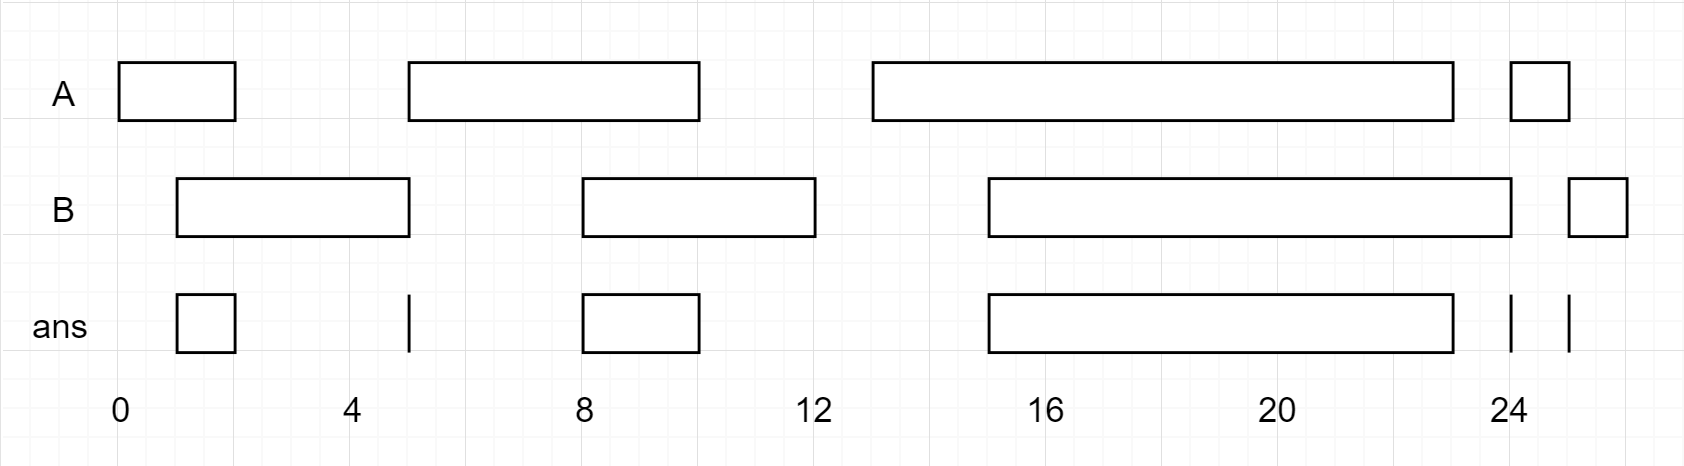
\includegraphics[width=0.7\linewidth]{images/lc0986_eg1}
\end{figure}
\item Example 2:
\begin{lstlisting}
interval_list1 = [[1,3],[5,9]]
interval_list2 = []
--> []
\end{lstlisting}
\end{itemize}

\subsection*{Solution}
\begin{lstlisting}
std::vector<std::vector<int>> intervalIntersection(
    std::vector<std::vector<int>>& interval_list1,
    std::vector<std::vector<int>>& interval_list2) {
  std::vector<std::vector<int>> intersections;
  int i = 0;
  int j = 0;
  while (i < interval_list1.size() && j < interval_list2.size()) {
    // check if there is an intersection
    int start_max = std::max(interval_list1[i][0], interval_list2[j][0]);
    int end_min = std::min(interval_list1[i][1], interval_list2[j][1]);
    if (start_max <= end_min) { intersections.push_back({start_max, end_min}); }
    // move the pointer with the smaller end
    if (interval_list1[i][1] < interval_list2[j][1]) {
      ++i;
    } else {
      ++j;
    }
  }
  return intersections;
}
\end{lstlisting}

\section{LC 0228 - Summary Ranges}\label{lc228}
You are given a \ul{unique} integer array {\colorbox{CodeBackground}{\lstinline|nums|}} \ul{sorted in ascending order}.\\

A range {\colorbox{CodeBackground}{\lstinline|[a,b]|}} is the set of all integers from {\colorbox{CodeBackground}{\lstinline|a|}} to {\colorbox{CodeBackground}{\lstinline|b|}} (inclusive).\\

Return the smallest sorted list of ranges that cover all the numbers in the array exactly. That is, each element of {\colorbox{CodeBackground}{\lstinline|nums|}} is covered by exactly one of the ranges, and there is no integer {\colorbox{CodeBackground}{\lstinline|x|}} such that {\colorbox{CodeBackground}{\lstinline|x|}} is in one of the ranges but not in {\colorbox{CodeBackground}{\lstinline|nums|}}.\\

Each range {\colorbox{CodeBackground}{\lstinline|[a,b]|}} in the list should be output as:
\begin{itemize}
\item {\colorbox{CodeBackground}{\lstinline|"a->b"|}} if {\colorbox{CodeBackground}{\lstinline|a != b|}}
\item {\colorbox{CodeBackground}{\lstinline|"a"|}} if {\colorbox{CodeBackground}{\lstinline|a == b|}}
\end{itemize}

Examples:
\begin{itemize}
\item {\colorbox{CodeBackground}{\lstinline|nums = [0,1,2,4,5,7] --> ["0->2","4->5","7"]|}}
\item {\colorbox{CodeBackground}{\lstinline|nums = [0,2,3,4,6,8,9] --> ["0","2->4","6","8->9"]|}}
\end{itemize}

\subsection*{Solution {\scriptsize\color{gray}\Coffeecup\hspace{1mm}Time $O(n)$, Space $O(1)$}}
\begin{lstlisting}
std::vector<std::string> summaryRanges(std::vector<int>& nums) {
  std::vector<std::string> ranges;
  if (nums.empty()) { return ranges; }
  for (int i = 0; i < nums.size(); ++i) {
    int start = nums[i];
    while (i + 1 < nums.size() && nums[i] + 1 == nums[i + 1]) { ++i; }
    if (start == nums[i]) {
      ranges.push_back(std::to_string(start));
    } else {
      ranges.push_back(std::to_string(start) + "->" + std::to_string(nums[i]));
    }
  }
  return ranges;
}
\end{lstlisting}

\section{LC 0128 - Maximum Number of Consecutive Elements}\label{lc0128}
Given an \ul{unsorted} array of integers {\colorbox{CodeBackground}{\lstinline|nums|}}, return the Maximum Number of Consecutive Elements.\\

Examples:
\begin{itemize}
	\item {\colorbox{CodeBackground}{\lstinline|nums = [100,4,200,1,3,2] --> 4 (1 - 4)|}}
	\item {\colorbox{CodeBackground}{\lstinline|nums = [0,3,7,2,5,8,4,6,0,1] --> 9 (0 - 8)|}}
\end{itemize}

\subsection*{Solution 1 - Hash Set {\scriptsize\color{gray}\Coffeecup\hspace{1mm}Time $O(n)$, Space $O(n)$}}
\begin{lstlisting}
int longestConsecutive(std::vector<int>& nums) {
  std::unordered_set<int> set(nums.begin(), nums.end());
  int max_len = 0;
  for (int num : nums) {
    // check if num is the start of a sequence
    if (set.find(num - 1) == set.end()) {
      int cur_num = num;
      int cur_len = 1;
      while (set.find(cur_num + 1) != set.end()) {
        ++cur_num;
        ++cur_len;
      }
      max_len = std::max(max_len, cur_len);
    }
  }
  return max_len;
}
\end{lstlisting}

\subsection*{Solution 2 - Sorting {\scriptsize\color{gray}\Coffeecup\hspace{1mm}Time $O(n\log n)$, Space $O(1)$}}
\begin{lstlisting}
int longestConsecutive(std::vector<int>& nums) {
  std::sort(nums.begin(), nums.end());
  auto it = std::unique(nums.begin(), nums.end());
  nums.erase(it, nums.end());
  int max_len = 0;
  int i = 0;
  for (int i = 0; i < nums.size(); ++i) {
    int cur_len = 1;
    while (i < nums.size() - 1 && nums[i] == nums[i + 1] - 1) {
      ++cur_len;
      ++i;
    }
    max_len = std::max(max_len, cur_len);
  }
  return max_len;
}
\end{lstlisting}

\section{LC 0370 - Range Addition}\label{lc0370}
\hyperref[sec:interval_range]{[Interval \& Range]}\\

You have an array {\colorbox{CodeBackground}{\lstinline|arr|}} of length {\colorbox{CodeBackground}{\lstinline|length|}} with all zeros, and you have some operation to apply on {\colorbox{CodeBackground}{\lstinline|arr|}}. \\

You also have a series of updates, represented in an array {\colorbox{CodeBackground}{\lstinline|updates|}} where {\colorbox{CodeBackground}{\lstinline|updates[i] = [startIdx_i, endIdx_i, inc_i]|}}.\\

In the {\colorbox{CodeBackground}{\lstinline|i|}}th operation, you increment all the elements {\colorbox{CodeBackground}{\lstinline|arr[startIdx_i], arr[startIdx_i + 1], ..., arr[endIdx_i]|}} by {\colorbox{CodeBackground}{\lstinline|inc_i|}}. \\

Return {\colorbox{CodeBackground}{\lstinline|arr|}} after applying all the {\colorbox{CodeBackground}{\lstinline|updates|}}.\\

\begin{itemize}
\item Example 1
\begin{lstlisting}
length = 5, updates = [[1,3,2],[2,4,3],[0,2,-2]] --> [-2,0,3,5,3]
\end{lstlisting}
\begin{figure}[H]
\centering
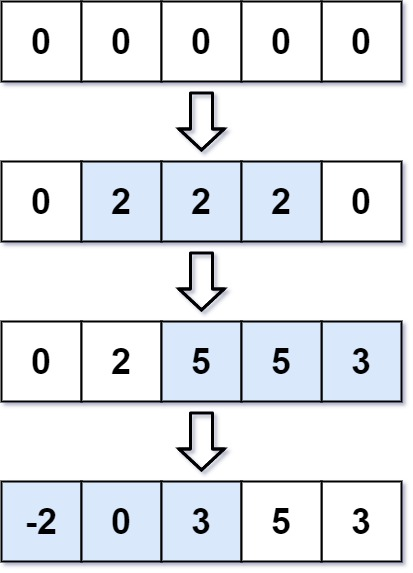
\includegraphics[width=0.2\linewidth]{images/lc0370_eg}
\label{fig:lc0370eg}
\end{figure}

\item Example 2
\begin{lstlisting}
length = 10, updates = [[2,4,6],[5,6,8],[1,9,-4]] --> [0,-4,2,2,2,4,4,-4,-4,-4]
\end{lstlisting}
\end{itemize}

\subsection*{Solution {\scriptsize\color{gray}\Coffeecup\hspace{1mm}Time $O(n)$, Space $O(1)$}}
\begin{lstlisting}
std::vector<int> getModifiedArray(int length, std::vector<std::vector<int>>& updates) {
  std::vector<int> arr(length, 0);
  for (const auto& update : updates) {
    int start_idx = update[0];
    int end_idx = update[1];
    int inc = update[2];
    arr[start_idx] += inc;
    if (end_idx + 1 < length) { arr[end_idx + 1] -= inc; }
  }
  for (int i = 1; i < length; ++i) { arr[i] += arr[i - 1]; }
  return arr;
}
\end{lstlisting}

\section{LC 0303 - Range Sum Query - Immutable}\label{lc0303}
\hyperref[sec:prefix_sum]{[Prefix Sum]}\\

Given a \ul{non-empty} integer array {\colorbox{CodeBackground}{\lstinline|nums|}}, handle multiple queries of the following type: \\

Calculate the sum of the elements of {\colorbox{CodeBackground}{\lstinline|nums|}} between indices {\colorbox{CodeBackground}{\lstinline|left|}} and {\colorbox{CodeBackground}{\lstinline|right|}} inclusive where {\colorbox{CodeBackground}{\lstinline|left <= right|}}.\\

Implement the {\colorbox{CodeBackground}{\lstinline|NumArray|}} class:
\begin{itemize}
\item {\colorbox{CodeBackground}{\lstinline|NumArray(int[] nums)|}} - Initializes the object with the integer array {\colorbox{CodeBackground}{\lstinline|nums|}}.
\item {\colorbox{CodeBackground}{\lstinline|int sumRange(int left, int right)|}} - Returns the sum of the elements of {\colorbox{CodeBackground}{\lstinline|nums|}} between indices {\colorbox{CodeBackground}{\lstinline|left|}} and {\colorbox{CodeBackground}{\lstinline|right|}} inclusive (i.e. {\colorbox{CodeBackground}{\lstinline|nums[left] + nums[left + 1] + ... + nums[right]|}}).
\end{itemize}

\subsection*{Solution 1 - Prefix Sum (size $n + 1$) {\scriptsize\color{gray}\Coffeecup\hspace{1mm}Time $O(n)$, Space $O(n)$}}
\begin{lstlisting}
class NumArray {
 public:
  NumArray(std::vector<int>& nums) {
    prefix_sum_.resize(nums.size() + 1, 0);
    for (int i = 0; i < nums.size(); ++i) { prefix_sum_[i + 1] = prefix_sum_[i] + nums[i]; }
  }

  int sumRange(int left, int right) { return prefix_sum_[right + 1] - prefix_sum_[left]; }

  std::vector<int> prefix_sum_;
};
\end{lstlisting}

\subsection*{Solution 2 - Prefix Sum (size $n$) {\scriptsize\color{gray}\Coffeecup\hspace{1mm}Time $O(n)$, Space $O(n)$}}
\begin{lstlisting}
class NumArray {
 public:
  NumArray(std::vector<int>& nums) {
    prefix_sum_.resize(nums.size(), 0);
    for (int i = 0; i < nums.size(); ++i) {
      prefix_sum_[i] = (i == 0 ? 0 : prefix_sum_[i - 1]) + nums[i];
    }
  }

  int sumRange(int left, int right) {
    return prefix_sum_[right] - (left == 0 ? 0 : prefix_sum_[left - 1]);
  }

 private:
  std::vector<int> prefix_sum_;
};
\end{lstlisting}

\subsection*{Related}
\begin{itemize}
\item \hyperref[lc0303]{LC 0303 - Range Sum Query - Immutable}
\item \hyperref[lc0304]{LC 0304 - Range Sum Query 2D - Immutable}
\end{itemize}

\section{LC 0238 - Product of Array Except Self}\label{lc0238}
\hyperref[sec:prefix_sum]{[Prefix Sum]}\\

Given an integer array {\colorbox{CodeBackground}{\lstinline|nums|}} ({\colorbox{CodeBackground}{\lstinline|nums.size() >= 2|}}), return an array {\colorbox{CodeBackground}{\lstinline|answer|}} such that {\colorbox{CodeBackground}{\lstinline|answer[i]|}} is equal to the product of all the elements of {\colorbox{CodeBackground}{\lstinline|nums|}} except {\colorbox{CodeBackground}{\lstinline|nums[i]|}}.\\

You must write an algorithm that runs in {\colorbox{CodeBackground}{\lstinline|O(n)|}} time and without using the division operation.\\

Examples:
\begin{itemize}
	\item {\colorbox{CodeBackground}{\lstinline|nums = [1,2,3,4] --> [24,12,8,6]|}}
	\item {\colorbox{CodeBackground}{\lstinline|nums = [-1,1,0,-3,3] --> [0,0,9,0,0]|}}
\end{itemize}

\subsection*{Solution 1 - Prefix \& Suffix Sum {\scriptsize\color{gray}\Coffeecup\hspace{1mm}Time $O(n)$, Space $O(n)$}}
\begin{lstlisting}
std::vector<int> productExceptSelf(std::vector<int>& nums) {
  int n = nums.size();
  std::vector<int> prefix_prod(n + 1, 1);
  for (int i = 0; i < n; ++i) { prefix_prod[i + 1] = prefix_prod[i] * nums[i]; }
  std::vector<int> suffix_prod(n + 1, 1);
  for (int i = n - 1; i >= 0; --i) { suffix_prod[i] = suffix_prod[i + 1] * nums[i]; }
  std::vector<int> res(n);
  for (int i = 0; i < n; ++i) { res[i] = prefix_prod[i] * suffix_prod[i + 1]; }
  return res;
}
\end{lstlisting}

\subsection*{Solution 1 - Prefix \& Suffix Sum, Optimized {\scriptsize\color{gray}\Coffeecup\hspace{1mm}Time $O(n)$, Space $O(n)$}}
\begin{lstlisting}
std::vector<int> productExceptSelf(std::vector<int>& nums) {
  int n = nums.size();
  std::vector<int> prefix_prod(n, 1);
  std::vector<int> suffix_prod(n, 1);
  for (int i = 1; i < n; ++i) { prefix_prod[i] = prefix_prod[i - 1] * nums[i - 1]; }
  for (int i = n - 2; i >= 0; --i) { suffix_prod[i] = suffix_prod[i + 1] * nums[i + 1]; }
  std::vector<int> res(n);
  for (int i = 0; i < n; ++i) { res[i] = prefix_prod[i] * suffix_prod[i]; }
  return res;
}
\end{lstlisting}

\section{LC 0560 - Subarray Sum Equals Target}\label{lc0560}
\hyperref[sec:prefix_sum]{[Prefix Sum]}\\

Given a \ul{non-empty} integer array {\colorbox{CodeBackground}{\lstinline|nums|}} and an integer {\colorbox{CodeBackground}{\lstinline|target|}}, return the number of subarrays whose sum equals to {\colorbox{CodeBackground}{\lstinline|target|}}.\\

Examples:
\begin{itemize}
\item {\colorbox{CodeBackground}{\lstinline|nums = [1,1,1], target = 2 --> 2|}}
\item {\colorbox{CodeBackground}{\lstinline|nums = [1,2,3], target = 3 --> 2|}}
\end{itemize}

\subsection*{*Solution 1 - Prefix Sum (Time Limit Exceeded) {\scriptsize\color{gray}\Coffeecup\hspace{1mm}Time $O(n^2)$, Space $O(n)$}}
\begin{lstlisting}
int subarraySum(std::vector<int>& nums, int target) {
  std::vector<int> prefix_sum(nums.size() + 1, 0);
  for (int i = 1; i <= nums.size(); ++i) { prefix_sum[i] = prefix_sum[i - 1] + nums[i - 1]; }
  int num_subarray = 0;
  for (int i = 0; i < nums.size(); ++i) {
    for (int j = i + 1; j <= nums.size(); ++j) {
      if (prefix_sum[j] - prefix_sum[i] == target) { ++num_subarray; }
    }
  }
  return num_subarray;
}

\end{lstlisting}

\subsection*{Solution 2 - Prefix Sum + Hash Map {\scriptsize\color{gray}\Coffeecup\hspace{1mm}Time $O(n)$, Space $O(n)$}}
\begin{lstlisting}
int subarraySum(std::vector<int>& nums, int target) {
  std::unordered_map<int, int> acc_sum2freq;
  int num_subarray = 0;
  int acc_sum = 0;
  acc_sum2freq[0] = 1;
  for (int num : nums) {
    acc_sum += num;
    if (acc_sum2freq.find(acc_sum - target) != acc_sum2freq.end()) {
      num_subarray += acc_sum2freq[acc_sum - target];
    }
    ++acc_sum2freq[acc_sum];
  }
  return num_subarray;
}
\end{lstlisting}

\subsection*{Related - Hash Map For Searching Two Related Elements}
\begin{itemize}
\item \hyperref[lc0001]{LC 0001 - Two Sum}
\item \hyperref[lc0560]{LC 0560 - Subarray Sum Equals Target}
\item \hyperref[lc0523]{LC 0523 - Subarray Sum is Multiple of Target}
\item \hyperref[lc0525]{LC 0525 - Binary Subarray with Equal Zeros and Ones}
\end{itemize}

\section{LC 0523 - Subarray Sum is Multiple of Target}\label{lc0523}
\hyperref[sec:prefix_sum]{[Prefix Sum]}\\

Given a \ul{non-empty} integer array {\colorbox{CodeBackground}{\lstinline|nums|}} ({\colorbox{CodeBackground}{\lstinline|nums[i] >= 0|}}) and an integer {\colorbox{CodeBackground}{\lstinline|target|}} ({\colorbox{CodeBackground}{\lstinline|target >= 1|}}), return {\colorbox{CodeBackground}{\lstinline|true|}} if {\colorbox{CodeBackground}{\lstinline|nums|}} has a \ul{good subarray} or {\colorbox{CodeBackground}{\lstinline|false|}} otherwise.\\

A \ul{good subarray} is a subarray where:
\begin{itemize}
\item its length is at least two, and
\item the sum of the elements of the subarray is a multiple of {\colorbox{CodeBackground}{\lstinline|target|}}.
\end{itemize}

Note that an integer {\colorbox{CodeBackground}{\lstinline|x|}} is a multiple of {\colorbox{CodeBackground}{\lstinline|target|}} if there exists an integer {\colorbox{CodeBackground}{\lstinline|n|}} such that {\colorbox{CodeBackground}{\lstinline|x = n * k|}}. {\colorbox{CodeBackground}{\lstinline|0|}} is always a multiple of {\colorbox{CodeBackground}{\lstinline|target|}}.\\

Examples:
\begin{itemize}
\item {\colorbox{CodeBackground}{\lstinline|nums = [23,2,4,6,7], target = 6 --> true ([2,4])|}}
\item {\colorbox{CodeBackground}{\lstinline|nums = [23,2,6,4,7], target = 6 --> true ([23,2,6,4,7])|}}
\item {\colorbox{CodeBackground}{\lstinline|nums = [23,2,6,4,7], target = 13 --> false|}}
\end{itemize}

\subsection*{*Solution 1 - Prefix Sum (Time Limit Exceeded) {\scriptsize\color{gray}\Coffeecup\hspace{1mm}Time $O(n^2)$, Space $O(n)$}}
\begin{lstlisting}
bool checkSubarraySum(std::vector<int>& nums, int target) {
  std::vector<int> prefix_sum(nums.size() + 1, 0);
  for (int i = 1; i <= nums.size(); ++i) { prefix_sum[i] = prefix_sum[i - 1] + nums[i - 1]; }
  for (int i = 0; i < nums.size() - 1; ++i) {
    for (int j = i + 2; j <= nums.size(); ++j) {
      if ((prefix_sum[j] - prefix_sum[i]) % target == 0) { return true; }
    }
  }
  return false;
}
\end{lstlisting}

\subsection*{Solution 2 - Prefix Sum + Hash Map {\scriptsize\color{gray}\Coffeecup\hspace{1mm}Time $O(n)$, Space $O(n)$}}
\begin{lstlisting}
bool checkSubarraySum(std::vector<int>& nums, int target) {
  std::unordered_map<int, int> acc_rem2idx;
  int acc_sum = 0;
  acc_rem2idx[0] = -1;
  for (int i = 0; i < nums.size(); ++i) {
    acc_sum += nums[i];
    int acc_rem = acc_sum % target;
    if (acc_rem2idx.find(acc_rem) != acc_rem2idx.end()) {
      if (i - acc_rem2idx[acc_rem] >= 2) { return true; }
    } else {  // store the earliest index for each remainder
      acc_rem2idx[acc_rem] = i;
    }
  }
  return false;
}
\end{lstlisting}

\subsection*{Related - Hash Map For Searching Two Related Elements}
\begin{itemize}
\item \hyperref[lc0001]{LC 0001 - Two Sum}
\item \hyperref[lc0560]{LC 0560 - Subarray Sum Equals Target}
\item \hyperref[lc0523]{LC 0523 - Subarray Sum is Multiple of Target}
\item \hyperref[lc0525]{LC 0525 - Binary Subarray with Equal Zeros and Ones}
\end{itemize}

\section{LC 0525 - Binary Subarray with Equal Zeros and Ones}\label{lc0525}
\hyperref[sec:prefix_sum]{[Prefix Sum]}\\

Given a \ul{non-empty} binary array {\colorbox{CodeBackground}{\lstinline|nums|}}, return the maximum length of a subarray with an equal number of {\colorbox{CodeBackground}{\lstinline|0|}} and {\colorbox{CodeBackground}{\lstinline|1|}}.\\

\begin{itemize}
\item {\colorbox{CodeBackground}{\lstinline|nums = [0,1] --> 2|}}
\item {\colorbox{CodeBackground}{\lstinline|nums = [0,1,0] --> 2|}}
\end{itemize}

\subsection*{Solution - Prefix Sum {\scriptsize\color{gray}\Coffeecup\hspace{1mm}Time $O(n)$, Space $O(n)$}}
\begin{lstlisting}
int findMaxLength(std::vector<int>& nums) {
  std::unordered_map<int, int> acc_sum2idx;
  int max_len = 0;
  int acc_sum = 0;
  acc_sum2idx[0] = -1;
  for (int i = 0; i < nums.size(); i++) {
    acc_sum += (nums[i] == 0) ? -1 : 1;
    if (acc_sum2idx.find(acc_sum) != acc_sum2idx.end()) {
      max_len = std::max(max_len, i - acc_sum2idx[acc_sum]);
    } else {  // store the earliest index for each acc_sum
      acc_sum2idx[acc_sum] = i;
    }
  }
  return max_len;
}
\end{lstlisting}

\subsection*{Related - Hash Map For Searching Two Related Elements}
\begin{itemize}
\item \hyperref[lc0001]{LC 0001 - Two Sum}
\item \hyperref[lc0560]{LC 0560 - Subarray Sum Equals Target}
\item \hyperref[lc0523]{LC 0523 - Subarray Sum is Multiple of Target}
\item \hyperref[lc0525]{LC 0525 - Binary Subarray with Equal Zeros and Ones}
\end{itemize}

\section{LC 0209 - Shortest Subarray Sum Greater or Equal to Target}\label{lc0209}
{\hyperref[sec:sliding_window]{[Sliding Window]}}

\begin{tcolorbox}
\begin{itemize}
\item Find the \ul{shortest subarray} whose sum is greater or equal to {\colorbox{CodeBackground}{\lstinline|target|}} in the given \ul{array}.
\end{itemize}
\end{tcolorbox}

Given a \ul{non-empty} array of integers {\colorbox{CodeBackground}{\lstinline|nums|}} ({\colorbox{CodeBackground}{\lstinline|nums[i] >= 1|}}) and a integer {\colorbox{CodeBackground}{\lstinline|target|}} ({\colorbox{CodeBackground}{\lstinline|target >= 1|}}), return the minimal length of a \ul{subarray} whose sum is greater than or equal to {\colorbox{CodeBackground}{\lstinline|target|}}. If there is no such subarray, return {\colorbox{CodeBackground}{\lstinline|0|}} instead.\\

Examples:
\begin{itemize}
\item {\colorbox{CodeBackground}{\lstinline|target = 7, nums = [2,3,1,2,4,3] --> 2 ([4,3])|}}
\item {\colorbox{CodeBackground}{\lstinline|target = 4, nums = [1,4,4] --> 1|}}
\item {\colorbox{CodeBackground}{\lstinline|target = 11, nums = [1,1,1,1,1,1,1,1] --> 0|}}
\end{itemize}

\subsection*{Solution - Sliding Window {\scriptsize\color{gray}\Coffeecup\hspace{1mm}Time $O(n)$, Space $O(1)$}}
\begin{lstlisting}
int minSubArrayLen(int target, std::vector<int>& nums) {
  int min_len = std::numeric_limits<int>::max();
  int sum = 0;
  int left = 0;
  for (int right = 0; right < nums.size(); ++right) {
    sum += nums[right];
    while (sum >= target) {
      min_len = std::min(min_len, right - left + 1);
      sum -= nums[left];
      ++left;
    }
  }
  return min_len == std::numeric_limits<int>::max() ? 0 : min_len;
}
\end{lstlisting}

\section{LC 1658 - Minimum Operations to Reduce X to Zero}\label{lc1658}
{\hyperref[sec:sliding_window]{[Sliding Window]}}

\begin{tcolorbox}
\begin{itemize}
\item Find the \ul{longest subarray} whose sum is equal to a target in the given \ul{array}.
\end{itemize}
\end{tcolorbox}

You are given a \ul{non-empty} integer array {\colorbox{CodeBackground}{\lstinline|nums|}} ({\colorbox{CodeBackground}{\lstinline|nums[i] >= 1|}}) and an integer {\colorbox{CodeBackground}{\lstinline|x|}} ({\colorbox{CodeBackground}{\lstinline|x >= 1|}}). \\

In one operation, you can either remove the \ul{leftmost} or the \ul{rightmost} element from {\colorbox{CodeBackground}{\lstinline|nums|}} and subtract its value from {\colorbox{CodeBackground}{\lstinline|x|}}. \\

Return the minimum number of operations to reduce {\colorbox{CodeBackground}{\lstinline|x|}} to \ul{exactly {\colorbox{CodeBackground}{\lstinline|0|}}} if it is possible, otherwise, return {\colorbox{CodeBackground}{\lstinline|-1|}}.\\

Examples:
\begin{itemize}
\item {\colorbox{CodeBackground}{\lstinline|nums = [1,1,4,2,3], x = 5 --> 2|}}
\item {\colorbox{CodeBackground}{\lstinline|nums = [5,6,7,8,9], x = 4 --> -1|}}
\item {\colorbox{CodeBackground}{\lstinline|nums = [3,2,20,1,1,3], x = 10 --> 5|}}
\end{itemize}

\subsection*{Solution - Sliding Window {\scriptsize\color{gray}\Coffeecup\hspace{1mm}Time $O(n)$, Space $O(1)$}}
\begin{lstlisting}
int minOperations(std::vector<int>& nums, int x) {
  int target = std::accumulate(nums.begin(), nums.end(), 0) - x;
  if (target < 0) { return -1; }
  int max_len = -1;
  int sum = 0;
  int left = 0;
  for (int right = 0; right < nums.size(); ++right) {
    sum += nums[right];
    while (sum > target) {
      sum -= nums[left];
      ++left;
    }
    if (sum == target) { max_len = std::max(max_len, right - left + 1); }
  }
  return max_len == -1 ? -1 : nums.size() - max_len;
}
\end{lstlisting}

\section{LC 1838 - Frequency of the Most Frequent Element after Increment}\label{lc1838}
{\hyperref[sec:sliding_window]{[Sliding Window]}}\\

You are given a \ul{non-empty} integer array {\colorbox{CodeBackground}{\lstinline|nums|}} ({\colorbox{CodeBackground}{\lstinline|nums[i] >= 1|}}) and an integer {\colorbox{CodeBackground}{\lstinline|k|}} ({\colorbox{CodeBackground}{\lstinline|k >= 1|}}). \\

In one operation, you can choose an index of {\colorbox{CodeBackground}{\lstinline|nums|}} and increment the element at that index by {\colorbox{CodeBackground}{\lstinline|1|}}.\\

Return the maximum possible frequency of an element after performing at most {\colorbox{CodeBackground}{\lstinline|k|}} operations.\\

Examples:
\begin{itemize}
\item {\colorbox{CodeBackground}{\lstinline|nums = [1,2,4], k = 5 --> 3 ([4,4,4])|}}
\item {\colorbox{CodeBackground}{\lstinline|nums = [1,4,8,13], k = 5 --> 2|}}\\
There are multiple optimal solutions:\\
- Increment the first element three times to make {\colorbox{CodeBackground}{\lstinline|nums = [4,4,8,13]|}}. \\
- Increment the second element four times to make {\colorbox{CodeBackground}{\lstinline|nums = [1,8,8,13]|}}. \\
- Increment the third element five times to make {\colorbox{CodeBackground}{\lstinline|nums = [1,4,13,13]|}}.
\item {\colorbox{CodeBackground}{\lstinline|nums = [3,9,6], k = 2 --> 1|}}
\end{itemize}

\subsection*{Solution - Sliding Window {\scriptsize\color{gray}\Coffeecup\hspace{1mm}Time $O(n)$, Space $O(1)$}}
We maintain a window in which the total number of operations required to equalize all elements does not surpass {\colorbox{CodeBackground}{\lstinline|k|}}.
\begin{lstlisting}
int maxFrequency(std::vector<int>& nums, int k) {
  std::sort(nums.begin(), nums.end());
  long num_op = 0;
  int max_freq = 1;
  int left = 0;
  for (int right = 1; right < nums.size(); ++right) {
    num_op += static_cast<long>(nums[right] - nums[right - 1]) * (right - left);
    while (num_op > k) {
      num_op -= nums[right] - nums[left];
      ++left;
    }
    max_freq = std::max(max_freq, right - left + 1);
  }
  return max_freq;
}
\end{lstlisting}

\section{LC 0239 - Sliding Window Maximum}\label{lc0239}
{\hyperref[sec:sliding_window]{[Sliding Window]}}\\

You are given a \ul{non-empty} array of integers {\colorbox{CodeBackground}{\lstinline|nums|}}, there is a sliding window of size {\colorbox{CodeBackground}{\lstinline|k|}} ({\colorbox{CodeBackground}{\lstinline|k >= 1|}}) which is moving from the very left of the array to the very right. You can only see the {\colorbox{CodeBackground}{\lstinline|k|}} numbers in the window. Each time the sliding window moves right by one position.\\

Return the list of max element for each window. \\

Examples:
\begin{itemize}
\item {\colorbox{CodeBackground}{\lstinline|nums = [1,3,-1,-3,5,3,6,7], k = 3 --> [3,3,5,5,6,7]|}}
\begin{lstlisting}
     Window Position           Max
--------------------------    -----
[1  3  -1] -3  5  3  6  7       3
 1 [3  -1  -3] 5  3  6  7       3
 1  3 [-1  -3  5] 3  6  7       5
 1  3  -1 [-3  5  3] 6  7       5
 1  3  -1  -3 [5  3  6] 7       6
 1  3  -1  -3  5 [3  6  7]      7
\end{lstlisting}
\item {\colorbox{CodeBackground}{\lstinline|nums = [1], k = 1 --> [1]|}}
\end{itemize}

\subsection*{Solution 1 - Brute Force}
\begin{lstlisting}
std::vector<int> maxSlidingWindow(std::vector<int>& nums, int k) {
  std::vector<int> max_elements;
  for (int i = 0; i < nums.size() - k + 1; ++i) {
    int maximum = std::numeric_limits<int>::min();
    for (int j = i; j < i + k; ++j) { maximum = std::max(maximum, nums[j]); }
    max_elements.push_back(maximum);
  }
  return max_elements;
}
\end{lstlisting}

\subsection*{Solution 2 - Deque}
\begin{lstlisting}
std::vector<int> maxSlidingWindow(std::vector<int>& nums, int k) {
  std::vector<int> max_elements;
  std::deque<int> window;
  for (int i = 0; i < nums.size(); ++i) {
    // Remove the indices that are out of the current window
    while (!window.empty() && window.front() <= i - k) { window.pop_front(); }

    // Remove indices from the back that are less than the current element
    while (!window.empty() && nums[i] >= nums[window.back()]) { window.pop_back(); }

    // Add the current index to the deque
    window.push_back(i);

    // If we've hit k elements, add the front of the deque to the result, as it's the max
    if (i >= k - 1) { max_elements.push_back(nums[window.front()]); }
  }

  return max_elements;
}
\end{lstlisting}

\section{LC 0480 - Sliding Window Median}\label{lc0480}
{\hyperref[sec:sliding_window]{[Sliding Window]}}\\

You are given a \ul{non-empty} integer array nums and an integer {\colorbox{CodeBackground}{\lstinline|k|}} ({\colorbox{CodeBackground}{\lstinline|k >= 1|}}). There is a sliding window of size {\colorbox{CodeBackground}{\lstinline|k|}} which is moving from the very left of the array to the very right. You can only see the {\colorbox{CodeBackground}{\lstinline|k|}} numbers in the window. Each time the sliding window moves right by one position.\\

Return the median array for each window in the original array. Answers within {\colorbox{CodeBackground}{\lstinline|10^-5|}} of the actual value will be accepted.\\

Examples:
\begin{itemize}
\item {\colorbox{CodeBackground}{\lstinline|nums = [1,3,-1,-3,5,3,6,7], k = 3 --> [1.00000,-1.00000,-1.00000,3.00000,5.00000,6.00000]|}}
\begin{lstlisting}
    Window Position            Median
--------------------------     -----
[1  3  -1] -3  5  3  6  7        1
 1 [3  -1  -3] 5  3  6  7       -1
 1  3 [-1  -3  5] 3  6  7       -1
 1  3  -1 [-3  5  3] 6  7        3
 1  3  -1  -3 [5  3  6] 7        5
 1  3  -1  -3  5 [3  6  7]       6
\end{lstlisting}
\item {\colorbox{CodeBackground}{\lstinline|nums = [1,2,3,4,2,3,1,4,2], k = 3 --> [2.00000,3.00000,3.00000,3.00000,2.00000,3.00000,2.00000]|}}
\end{itemize}

\section{LC 0274 - H-Index}
Given an array of integers {\colorbox{CodeBackground}{\lstinline|citations|}} where {\colorbox{CodeBackground}{\lstinline|citations[i]|}} is the number of citations a researcher received for their {\colorbox{CodeBackground}{\lstinline|i|}}th paper, return the researcher's \ul{h-index}.\\

The \ul{h-index} is defined as the maximum value of {\colorbox{CodeBackground}{\lstinline|h|}} such that the given researcher has published at least {\colorbox{CodeBackground}{\lstinline|h|}} papers that have each been cited at least {\colorbox{CodeBackground}{\lstinline|h|}} times.\\

Examples:
\begin{itemize}
	\item {\colorbox{CodeBackground}{\lstinline|citations = [3,0,6,1,5] --> 3|}}
	\item {\colorbox{CodeBackground}{\lstinline|citations = [1,3,1] --> 1|}}
\end{itemize}

\subsection*{Solution}
\begin{lstlisting}
int hIndex(std::vector<int>& citations) {
	std::sort(citations.begin(), citations.end(), std::greater<int>());
	int h_idx = 0;
	for (int i = 0; i < citations.size(); ++i) {
		if (citations[i] >= i + 1) {
			h_idx = i + 1;
		} else {
			break;
		}
	}
	return h_idx;
}
\end{lstlisting}

\section{LC 0042 - Trapping Rain Water}
Given {\colorbox{CodeBackground}{\lstinline|n|}} ({\colorbox{CodeBackground}{\lstinline|n >= 1|}}) non-negative integers representing an elevation map where the width of each bar is {\colorbox{CodeBackground}{\lstinline|1|}}, compute how much water it can trap after raining.\\

Example: {\colorbox{CodeBackground}{\lstinline|height = [0,1,0,2,1,0,1,3,2,1,2,1] --> 6|}}
\begin{figure}[H]
\centering
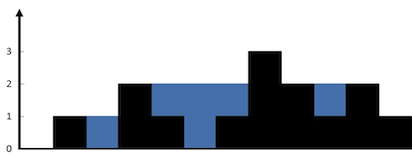
\includegraphics[width=0.4\linewidth]{images/lc0042_eg}
\end{figure}

\subsection*{Solution - Brute Force (Time Limit Exceeded)}\label{solution:lc0042_brute_force}
\begin{lstlisting}
int trap(std::vector<int>& heights) {
  int trapped_water = 0;
  for (int i = 1; i < heights.size() - 1; ++i) {
    int left_max_h = *std::max_element(heights.begin(), heights.begin() + i);
    int right_max_h = *std::max_element(heights.begin() + i + 1, heights.end());
    int height = std::min(left_max_h, right_max_h) - heights[i];
    trapped_water += height > 0 ? height : 0;
  }
  return trapped_water;
}
\end{lstlisting}

\subsection*{Solution - Brute Force, Optimized}\label{solution:lc0042_brute_force_optimized_1}
\begin{lstlisting}
int trap(std::vector<int>& heights) {
  if (heights.size() <= 2) { return 0; }
  int n = heights.size();
  std::vector<int> max_left_height(n, 0);
  std::vector<int> max_right_height(n, 0);
  max_left_height[0] = heights[0];
  for (int i = 1; i < n; ++i) {
    max_left_height[i] = std::max(heights[i], max_left_height[i - 1]);
  }
  max_right_height[n - 1] = heights[n - 1];
  for (int i = n - 2; i >= 0; --i) {
    max_right_height[i] = std::max(heights[i], max_right_height[i + 1]);
  }
  int trapped_water = 0;
  for (int i = 0; i < n; i++) {
    int height = std::min(max_left_height[i], max_right_height[i]) - heights[i];
    if (height > 0) { trapped_water += height; }
  }
  return trapped_water;
}
\end{lstlisting}

\subsection*{Solution - Brute Force, Optimized}\label{solution:lc0042_brute_force_optimized_2}
\begin{lstlisting}
int trap(std::vector<int>& heights) {
  int left_max_h = 0;
  int right_max_h = 0;
  int trapped_water = 0;
  int left = 0;
  int right = heights.size() - 1;
  while (left < right) {
    left_max_h = std::max(left_max_h, heights[left]);
    right_max_h = std::max(right_max_h, heights[right]);
    if (left_max_h < right_max_h) {
      trapped_water += left_max_h - heights[left];
      left++;
    } else {
      trapped_water += right_max_h - heights[right];
      right--;
    }
  }
  return trapped_water;
}
\end{lstlisting}

\subsection*{Other Solutions}
\begin{itemize}
%\item \hyperref[solution:lc0042_brute_force]{Brute Force (Time Limit Exceeded)}
%\item \hyperref[solution:lc0042_brute_force_optimized_1]{Brute Force, Optimized 1}
%\item \hyperref[solution:lc0042_brute_force_optimized_2]{Brute Force, Optimized 2}
\item \hyperref[solution:lc0042_monotonic_stack]{Monotonic Stack}
\end{itemize}

\chapter{String}
\section{LC 0028 - Find the Index of the First Occurrence in a String}
Given two \ul{non-empty} strings {\colorbox{CodeBackground}{\lstinline|needle|}} and {\colorbox{CodeBackground}{\lstinline|haystack|}}, return the index of the first occurrence of {\colorbox{CodeBackground}{\lstinline|needle|}} in {\colorbox{CodeBackground}{\lstinline|haystack|}}, or {\colorbox{CodeBackground}{\lstinline|-1|}} if {\colorbox{CodeBackground}{\lstinline|needle|}} is not part of {\colorbox{CodeBackground}{\lstinline|haystack|}}.\\

{\colorbox{CodeBackground}{\lstinline|haystack|}} and {\colorbox{CodeBackground}{\lstinline|needle|}} consist of only \ul{lowercase English characters}.\\

Examples:
\begin{itemize}
	\item {\colorbox{CodeBackground}{\lstinline|haystack = "sadbutsad", needle = "sad" --> 0|}}
	\item {\colorbox{CodeBackground}{\lstinline|haystack = "leetcode", needle = "leeto" --> -1|}}
\end{itemize}

\subsection*{Solution 1 - {\colorbox{CodeBackground}{\lstinline|std::string::find()|}}}
\begin{lstlisting}
int strStr(std::string haystack, std::string needle) {
	int pos = haystack.find(needle);
	if (pos != std::string::npos) {
		return pos;
	} else {
		return -1;
	}
}
\end{lstlisting}

\subsection*{Solution 2}
\begin{lstlisting}
int strStr(const std::string& haystack, const std::string& needle) {
  int n = haystack.size();
  int m = needle.size();
  for (int i = 0; i <= n - m; ++i) {
    if (haystack.substr(i, m) == needle) { return i; }
  }
  return -1;
}
\end{lstlisting}

\section{LC 0125 - Valid Palindrome}\label{lc0125}
Given a \ul{non-empty} string {\colorbox{CodeBackground}{\lstinline|s|}}, return {\colorbox{CodeBackground}{\lstinline|true|}} if it is a \ul{palindrome}, or {\colorbox{CodeBackground}{\lstinline|false|}} otherwise.\\

A phrase is a \ul{palindrome} if, after converting all uppercase letters into lowercase letters and removing all non-alphanumeric characters, it reads the same forward and backward.\\

{\colorbox{CodeBackground}{\lstinline|s|}} consists only of \ul{printable ASCII characters}.\\

Examples:
\begin{itemize}
\item {\colorbox{CodeBackground}{\lstinline|s = "A man, a plan, a canal: Panama" --> true|}}
\item {\colorbox{CodeBackground}{\lstinline|s = "race a car" --> false|}}
\item {\colorbox{CodeBackground}{\lstinline|s = " " --> true|}}
\end{itemize}

\subsection*{Solution}
\begin{lstlisting}
bool isPalindrome(std::string s) {
	auto left = s.begin();
	auto right = s.end() - 1;
	while (left < right) {
		if (!std::isalnum(*left)) {
			++left;
			continue;
		}
		if (!std::isalnum(*right)) {
			--right;
			continue;
		}
		if (std::tolower(*left) != std::tolower(*right)) { return false; }
		++left;
		--right;
	}
	return true;
}
\end{lstlisting}

\subsection*{Related - Palindrome}
\begin{itemize}
	\item \hyperref[lc0125]{LC 0125 - Valid Palindrome}
 	\item \hyperref[lc0680]{LC 0680 - Valid Palindrome II}
	\item \hyperref[lc0647]{LC 0647 - Palindromic Substrings}
	\item \hyperref[lc0005]{LC 0005 - Longest Palindromic Substring}
	\item \hyperref[lc0516]{LC 0516 - Longest Palindromic Subsequence}
\end{itemize}

\section{LC 0680 - Valid Palindrome II}\label{lc0680}
Given a \ul{non-empty} string {\colorbox{CodeBackground}{\lstinline|s|}}, return {\colorbox{CodeBackground}{\lstinline|true|}} if the {\colorbox{CodeBackground}{\lstinline|s|}} can be \ul{palindrome} after \ul{deleting at most one character} from it.\\

{\colorbox{CodeBackground}{\lstinline|s|}} consists of \ul{lowercase English letters}.

\subsection*{Solution}
\begin{lstlisting}
bool validPalindrome(std::string s) {
  int left = 0;
  int right = s.size() - 1;

  auto IsPalindrome = [&s](int l, int r) {
    while (l < r) {
      if (s[l] != s[r]) { return false; }
      ++l;
      --r;
    }
    return true;
  };

  while (left < right) {
    if (s[left] != s[right]) {
      return IsPalindrome(left + 1, right) || IsPalindrome(left, right - 1);
    }
    ++left;
    --right;
  }
  return true;
}
\end{lstlisting}

\subsection*{Related - Palindrome}
\begin{itemize}
	\item \hyperref[lc0125]{LC 0125 - Valid Palindrome}
 	\item \hyperref[lc0680]{LC 0680 - Valid Palindrome II}
	\item \hyperref[lc0647]{LC 0647 - Palindromic Substrings}
	\item \hyperref[lc0005]{LC 0005 - Longest Palindromic Substring}
	\item \hyperref[lc0516]{LC 0516 - Longest Palindromic Subsequence}
\end{itemize}

\section{LC 0392 - Is Subsequence}\label{lc0392}
Given two strings {\colorbox{CodeBackground}{\lstinline|s|}} and {\colorbox{CodeBackground}{\lstinline|t|}}, return {\colorbox{CodeBackground}{\lstinline|true|}} if {\colorbox{CodeBackground}{\lstinline|s|}} is a \ul{subsequence} of {\colorbox{CodeBackground}{\lstinline|t|}}, or {\colorbox{CodeBackground}{\lstinline|false|}} otherwise.\\

{\colorbox{CodeBackground}{\lstinline|s|}} and {\colorbox{CodeBackground}{\lstinline|t|}} consist only of \ul{lowercase English letters}.\\

Examples:
\begin{itemize}
	\item {\colorbox{CodeBackground}{\lstinline|s = "abc", t = "ahbgdc" --> true|}}
	\item {\colorbox{CodeBackground}{\lstinline|s = "axc", t = "ahbgdc" --> false|}}
\end{itemize}

\subsection*{Solution 1}
\begin{lstlisting}
bool isSubsequence(std::string s, std::string t) {
	int i = 0;
	int j = 0;
	while (i < s.size() && j < t.size()) {
		if (s[i] == t[j]) { ++i; }
		++j;
	}
	return i == s.size();
}
\end{lstlisting}

\subsection*{Solution 2}
\begin{lstlisting}
bool isSubsequence(std::string s, std::string t) {
  int i = 0;
  int j = 0;
  while (i < s.size()) {
    while (j < t.size() && t[j] != s[i]) { ++j; }
    if (j == t.size()) { return false; }
    ++i;
    ++j;
  }
  return true;
}
\end{lstlisting}

\subsection*{Related - Subsequence}
\begin{itemize}
	\item \hyperref[lc0392]{LC 0392 - Is Subsequence}
	\item \hyperref[lc1143]{LC 1143 - Longest Common Subsequence}
	\item \hyperref[lc0300]{LC 0300 - Longest Increasing Subsequence}
	\item \hyperref[lc0516]{LC 0516 - Longest Palindromic Subsequence}
\end{itemize}

\section{LC 0014 - Longest Common Prefix}
Write a function to find the \ul{longest common prefix} string among a \ul{non-empty} array of strings. If there is no common prefix, return an empty string {\colorbox{CodeBackground}{\lstinline|""|}}.\\

{\colorbox{CodeBackground}{\lstinline|strs[i]|}} consists of only \ul{lowercase English letters}.\\

Examples:
\begin{itemize}
\item {\colorbox{CodeBackground}{\lstinline|strs = ["flower","flow","flight"] --> "fl"|}}
\item {\colorbox{CodeBackground}{\lstinline|strs = ["dog","racecar","car"] --> ""|}}
\end{itemize}

\subsection*{Solution 1}
\begin{lstlisting}
std::string longestCommonPrefix(std::vector<std::string>& strs) {
  std::string prefix = strs[0];
  for (int i = 1; i < strs.size(); ++i) {
    while (strs[i].find(prefix) != 0) {
      prefix.erase(prefix.size() - 1);
      if (prefix.empty()) { return ""; }
    }
  }
  return prefix;
}
\end{lstlisting}

\subsection*{Solution 2 - Sort}
\begin{lstlisting}
std::string longestCommonPrefix(std::vector<std::string>& strs) {
  std::sort(begin(strs), end(strs));
  std::string prefix = "";
  std::string first = strs.front();
  std::string last = strs.back();
  for (int i = 0; i < first.size(); ++i) {
    if (first[i] == last[i]) {
      prefix.push_back(first[i]);
    } else {
      break;
    }
  }
  return prefix;
}
\end{lstlisting}

\section{LC 0058 - Length of Last Word}\label{lc0058}
Given a \ul{non-empty} string {\colorbox{CodeBackground}{\lstinline|s|}} consisting of words and spaces, return the length of the last word in the string.\\

{\colorbox{CodeBackground}{\lstinline|s|}} consists of only \ul{English letters} and \ul{spaces {\colorbox{CodeBackground}{\lstinline|' '|}}}.\\

Examples:
\begin{itemize}
	\item {\colorbox{CodeBackground}{\lstinline|s = "Hello World" --> 5|}}
	\item {\colorbox{CodeBackground}{\lstinline|s = "   fly me   to   the moon  " --> 4|}}
	\item {\colorbox{CodeBackground}{\lstinline|s = "luffy is still joyboy" --> 6|}}
\end{itemize}

\subsection*{Solution 1 - {\colorbox{CodeBackground}{\lstinline|std::istringstream|}}}
\begin{lstlisting}
int lengthOfLastWord(const std::string& s) {
  std::istringstream iss(s);
  std::string word;
  while (iss >> word) {}
  return word.size();
}
\end{lstlisting}

\subsection*{Solution 2 - Two Pointers}
\begin{lstlisting}
int lengthOfLastWord(std::string s) {
	// idx of last char of last word
	int j = s.size() - 1;
	while (j >= 0 && s[j] == ' ') { --j; }
	if (j < 0) { return 0; }
	// idx of first space before last word
	int i = j - 1;
	while (i >= 0 && s[i] != ' ') { --i; }
	return j - i;
}
\end{lstlisting}

\section{LC 0151 - Reverse Words in a String}\label{lc0151}
Given a \ul{non-empty} input string {\colorbox{CodeBackground}{\lstinline|s|}}, return a string of the words in reverse order concatenated by a single space. \\

Note that {\colorbox{CodeBackground}{\lstinline|s|}} may contain leading or trailing spaces or multiple spaces between two words. The returned string should only have a single space separating the words. Do not include any extra spaces.\\

{\colorbox{CodeBackground}{\lstinline|s|}} contains \ul{English letters (upper-case and lower-case)}, \ul{digits}, and \ul{spaces {\colorbox{CodeBackground}{\lstinline|' '|}}}, and there is at least one word in {\colorbox{CodeBackground}{\lstinline|s|}.\\

Examples:
\begin{itemize}
	\item {\colorbox{CodeBackground}{\lstinline|s = "the sky is blue" --> "blue is sky the"|}}
	\item {\colorbox{CodeBackground}{\lstinline|s = "  hello world  " --> "world hello"|}}
	\item {\colorbox{CodeBackground}{\lstinline|s = "a good   example" --> "example good a"|}}
\end{itemize}

\subsection*{Solution 1 - {\colorbox{CodeBackground}{\lstinline|std::istringstream|}}}
\begin{lstlisting}
std::string reverseWords(std::string s) {
  std::stack<std::string> stk;
  std::istringstream iss(s);
  std::string word;
  while (iss >> word) { stk.push(word); }
  std::string reversed_str;
  while (!stk.empty()) {
    reversed_str.append(stk.top());
    stk.pop();
    if (!stk.empty()) { reversed_str.append(" "); }
  }
  return reversed_str;
}
\end{lstlisting}

\subsection*{Solution 2 - Two Pointers}
\begin{lstlisting}
std::string reverseWords(std::string s) {
	std::string reversed_str = "";
	int j = s.size() - 1;
	while (j >= 0) {
		while (j >= 0 && s[j] == ' ') { --j; }
		if (j < 0) { break; }
		int i = j - 1;
		while (i >= 0 && s[i] != ' ') { --i; }
		reversed_str += s.substr(i + 1, j - i) + " ";
		j = i - 1;
	}
	return reversed_str.substr(0, reversed_str.size() - 1);
}
\end{lstlisting}

\section{LC 0383 - Ransom Note}\label{lc0383}
Given two \ul{non-empty} strings {\colorbox{CodeBackground}{\lstinline|ransomNote|}} and {\colorbox{CodeBackground}{\lstinline|magazine|}}, return {\colorbox{CodeBackground}{\lstinline|true|}} if {\colorbox{CodeBackground}{\lstinline|ransomNote|}} can be constructed by using the letters from {\colorbox{CodeBackground}{\lstinline|magazine|}} and {\colorbox{CodeBackground}{\lstinline|false|}} otherwise. Note that each letter in {\colorbox{CodeBackground}{\lstinline|magazine|}} can only be used once in {\colorbox{CodeBackground}{\lstinline|ransomNote|}}.\\

{\colorbox{CodeBackground}{\lstinline|ransomNote|}} and {\colorbox{CodeBackground}{\lstinline|magazine|}} consist of \ul{lowercase English letters}.\\

Examples:
\begin{itemize}
	\item {\colorbox{CodeBackground}{\lstinline|ransomNote = "a", magazine = "b" --> false|}}
	\item {\colorbox{CodeBackground}{\lstinline|ransomNote = "aa", magazine = "ab" --> false|}}
	\item {\colorbox{CodeBackground}{\lstinline|ransomNote = "aa", magazine = "aab" --> true|}}
\end{itemize}

\subsection*{Solution}
\begin{lstlisting}
bool canConstruct(std::string ransomNote, std::string magazine) {
  std::unordered_map<char, int> char2cnt;
  for (char c : magazine) { ++char2cnt[c]; }
  for (char c : ransomNote) {
    if (char2cnt[c] <= 0) {
      return false;
    } else {
      --char2cnt[c];
    }
  }
  return true;
}
\end{lstlisting}

\section{LC 0205 - Isomorphic Strings}\label{lc0205}
Given two \ul{non-empty} strings {\colorbox{CodeBackground}{\lstinline|s|}} and {\colorbox{CodeBackground}{\lstinline|t|}}, determine if they are \ul{isomorphic}.\\

Two strings {\colorbox{CodeBackground}{\lstinline|s|}} and {\colorbox{CodeBackground}{\lstinline|t|}} are \ul{isomorphic} if the characters in {\colorbox{CodeBackground}{\lstinline|s|}} can be replaced to get {\colorbox{CodeBackground}{\lstinline|t|}}.\\

Note:
\begin{itemize}
\item All occurrences of a character must be replaced with another character while preserving the order of characters.
\item No two characters may map to the same character, but a character may map to itself.
\item {\colorbox{CodeBackground}{\lstinline|t.size() == s.size()|}}
\item {\colorbox{CodeBackground}{\lstinline|s|}} and {\colorbox{CodeBackground}{\lstinline|t|}} consist of any \ul{valid ASCII character}.
\end{itemize}

Examples:
\begin{itemize}
	\item {\colorbox{CodeBackground}{\lstinline|s = "egg", t = "add" --> true|}}
	\item {\colorbox{CodeBackground}{\lstinline|s = "foo", t = "bar" --> false|}}
	\item {\colorbox{CodeBackground}{\lstinline|s = "paper", t = "title" --> true|}}
\end{itemize}

\subsection*{Solution - Bijection}
\begin{lstlisting}
bool isIsomorphic(std::string s, std::string t) {
  std::unordered_map<char, char> s2t;
  std::unordered_map<char, char> t2s;
  for (int i = 0; i < s.size(); ++i) {
    // s -> t
    if (s2t.find(s[i]) != s2t.end() && s2t[s[i]] != t[i]) { return false; }
    s2t[s[i]] = t[i];
    // t -> s
    if (t2s.find(t[i]) != t2s.end() && t2s[t[i]] != s[i]) { return false; }
    t2s[t[i]] = s[i];
  }
  return true;
}
\end{lstlisting}

\section{LC 0290 - Word Pattern}\label{lc0290}
Given a \ul{non-empty} {\colorbox{CodeBackground}{\lstinline|pattern|}} and a \ul{non-empty} string {\colorbox{CodeBackground}{\lstinline|s|}}, find if {\colorbox{CodeBackground}{\lstinline|s|}} matches the {\colorbox{CodeBackground}{\lstinline|pattern|}}.\\

A match means that there is a \ul{bijection} between a \ul{letter} in {\colorbox{CodeBackground}{\lstinline|pattern|}} and a \ul{non-empty word} in {\colorbox{CodeBackground}{\lstinline|s|}}.\\

Note that:
\begin{itemize}
\item {\colorbox{CodeBackground}{\lstinline|pattern|}} contains only \ul{lower-case English letters}.
\item {\colorbox{CodeBackground}{\lstinline|s|}} contains only \ul{lowercase English letters} and \ul{spaces {\colorbox{CodeBackground}{\lstinline|' '|}}}.
\item {\colorbox{CodeBackground}{\lstinline|s|}} does not contain any leading or trailing spaces.
\item All the words in {\colorbox{CodeBackground}{\lstinline|s|}} are separated by a single space.
\end{itemize}

Examples:
\begin{itemize}
	\item {\colorbox{CodeBackground}{\lstinline|pattern = "abba", s = "dog cat cat dog" --> true|}}
	\item {\colorbox{CodeBackground}{\lstinline|pattern = "abba", s = "dog cat cat fish" --> false|}}
	\item {\colorbox{CodeBackground}{\lstinline|pattern = "aaaa", s = "dog cat cat dog" --> false|}}
\end{itemize}

\subsection*{Solution}
\begin{lstlisting}
bool wordPattern(std::string pattern, std::string s) {
	std::unordered_map<char, std::string> char2word;
	std::unordered_map<std::string, char> word2char;
	std::istringstream iss(s);
	std::string word;
	for (char c : pattern) {
		if (!(iss >> word)) { return false; }
		if (char2word.find(c) != char2word.end() && char2word[c] != word) { return false; }
		char2word[c] = word;
		if (word2char.find(word) != word2char.end() && word2char[word] != c) { return false; }
		word2char[word] = c;
	}
	return !(iss >> word);
}
\end{lstlisting}

\section{LC 0242 - Valid Anagram}\label{lc0242}
Given two \ul{non-empty} strings {\colorbox{CodeBackground}{\lstinline|s|}} and {\colorbox{CodeBackground}{\lstinline|t|}}, return {\colorbox{CodeBackground}{\lstinline|true|}} if {\colorbox{CodeBackground}{\lstinline|t|}} is an \ul{anagram} of {\colorbox{CodeBackground}{\lstinline|s|}}, and {\colorbox{CodeBackground}{\lstinline|false|}} otherwise.\\

An \ul{anagram} is a word or phrase formed by rearranging the letters of a different word or phrase, typically using all the original letters exactly once.\\

{\colorbox{CodeBackground}{\lstinline|s|}} and {\colorbox{CodeBackground}{\lstinline|t|}} consist of \ul{lowercase English letters}.\\

Examples:
\begin{itemize}
	\item {\colorbox{CodeBackground}{\lstinline|s = "anagram", t = "nagaram" --> true|}}
	\item {\colorbox{CodeBackground}{\lstinline|s = "rat", t = "car" --> false|}}
\end{itemize}

\subsection*{Solution 1 - Sort}
\begin{lstlisting}
bool isAnagram(std::string s, std::string t) {
	std::sort(s.begin(), s.end());
	std::sort(t.begin(), t.end());
	return s == t;
}
\end{lstlisting}

\subsection*{Solution 2 - Hash Map}
\begin{lstlisting}
bool isAnagram(std::string s, std::string t) {
	if (s.length() != t.length()) { return false; }
	std::unordered_map<char, int> char2count;
	for (char c : s) { ++char2count[c]; }
	for (char c : t) {
		--char2count[c];
		if (char2count[c] < 0) { return false; }
	}
	return true;
}

\end{lstlisting}

\subsection*{Solution 3 - Array}
\begin{lstlisting}
bool isAnagram(std::string s, std::string t) {
	if (s.length() != t.length()) { return false; }
	std::vector<int> freq(256, 0);
	for (char c : s) { ++freq[c]; }
	for (char c : t) {
		--freq[c];
		if (freq[c] < 0) { return false; }
	}
	return true;
}
\end{lstlisting}

\subsection*{Related - Anagram}
\begin{itemize}
\item \hyperref[lc0242]{LC 0242 - Valid Anagram}
\item \hyperref[lc0049]{LC 0049 - Group Anagrams}
\item \hyperref[lc0438]{LC 0438 - Find All Anagrams in a String}
\end{itemize}

\section{LC 0049 - Group Anagrams}\label{lc0049}
Given an array of strings {\colorbox{CodeBackground}{\lstinline|strs|}} ({\colorbox{CodeBackground}{\lstinline|strs.size() >= 1|}}), group the \ul{anagrams} together. You can return the answer in any order.\\

An \ul{anagram} is a word or phrase formed by rearranging the letters of a different word or phrase, typically using all the original letters exactly once.\\

{\colorbox{CodeBackground}{\lstinline|strs[i]|}} consists of \ul{lowercase English letters}.\\

Examples:
\begin{itemize}
	\item {\colorbox{CodeBackground}{\lstinline|strs = ["eat","tea","tan","ate","nat","bat"] --> [["bat"],["nat","tan"],["ate","eat","tea"]]|}}
	\item {\colorbox{CodeBackground}{\lstinline|strs = [""] --> [[""]]|}}
	\item {\colorbox{CodeBackground}{\lstinline|strs = ["a"] --> [["a"]]|}}
\end{itemize}

\subsection*{Solution}
\begin{lstlisting}
std::vector<std::vector<std::string>> groupAnagrams(std::vector<std::string>& strs) {
	std::unordered_map<std::string, std::vector<std::string>> key2group;
	for (std::string& str : strs) {
		std::string key = str;
		std::sort(key.begin(), key.end());
		key2group[key].push_back(str);
	}
	std::vector<std::vector<std::string>> result;
	for (auto& pair : key2group) { result.push_back(pair.second); }
	return result;
}
\end{lstlisting}

\subsection*{Related - Anagram}
\begin{itemize}
\item \hyperref[lc0242]{LC 0242 - Valid Anagram}
\item \hyperref[lc0049]{LC 0049 - Group Anagrams}
\item \hyperref[lc0438]{LC 0438 - Find All Anagrams in a String}
\end{itemize}

\section{LC 0647 - Palindromic Substrings}\label{lc0647}
Given a \ul{non-empty} string {\colorbox{CodeBackground}{\lstinline|s|}}, return the number of \ul{palindromic substrings} in it.\\

{\colorbox{CodeBackground}{\lstinline|s|}} consists of \ul{lowercase English letters}.\\

Examples:
\begin{itemize}
	\item {\colorbox{CodeBackground}{\lstinline|s = "abc" --> 3|}}
	\item {\colorbox{CodeBackground}{\lstinline|s = "aaa" --> 6|}}
\end{itemize}

\subsection*{Solution - Expand Around Center}
\begin{lstlisting}
int countSubstrings(std::string s) {
	int total_count = 0;
	for (int i = 0; i < s.length(); i++) {
		total_count += CountPalindromesAroundCenter(s, i, i);
		total_count += CountPalindromesAroundCenter(s, i, i + 1);
	}
	return total_count;
}

int CountPalindromesAroundCenter(const std::string& s, int left, int right) {
	int count = 0;
	while (left >= 0 && right < s.length() && s[left] == s[right]) {
		--left;
		++right;
		++count;
	}
	return count;
}
\end{lstlisting}

\subsection*{Related - Palindrome}
\begin{itemize}
	\item \hyperref[lc0125]{LC 0125 - Valid Palindrome}
 	\item \hyperref[lc0680]{LC 0680 - Valid Palindrome II}
	\item \hyperref[lc0647]{LC 0647 - Palindromic Substrings}
	\item \hyperref[lc0005]{LC 0005 - Longest Palindromic Substring}
	\item \hyperref[lc0516]{LC 0516 - Longest Palindromic Subsequence}
\end{itemize}

\section{LC 0005 - Longest Palindromic Substring}\label{lc0005}
Given a \ul{non-empty} string {\colorbox{CodeBackground}{\lstinline|s|}}, return the longest \ul{palindromic substring} in {\colorbox{CodeBackground}{\lstinline|s|}}.\\

{\colorbox{CodeBackground}{\lstinline|s|}} consist of only \ul{digits} and \ul{English letters}.\\

Examples:
\begin{itemize}
	\item {\colorbox{CodeBackground}{\lstinline|"babad" --> "bab"\ \ or "aba"|}}
	\item {\colorbox{CodeBackground}{\lstinline|"cbbd" --> "bb"|}}
\end{itemize}

\subsection*{Solution - Expand Around Center}\label{solution:lc0005_expand_around_center}
\begin{lstlisting}
std::string longestPalindrome(std::string s) {
	int begin = 0;
	int max_len = 1;
	for (int i = 0; i < s.size(); i++) {
		int odd_len = LengthOfLongestPalindromAroundCenter(s, i, i);
		int even_len = LengthOfLongestPalindromAroundCenter(s, i, i + 1);
		int cur_len = std::max(odd_len, even_len);
		if (cur_len > max_len) {
			begin = i - (cur_len - 1) / 2;
			max_len = cur_len;
		}
	}
	return s.substr(begin, max_len);
}

int LengthOfLongestPalindromAroundCenter(const std::string& s, int left, int right) {
	while (left >= 0 && right < s.size() && s[left] == s[right]) {
		left--;
		right++;
	}
	return right - left - 1;
}
\end{lstlisting}

\subsection*{Other Solutions}
\begin{itemize}
%	\item \hyperref[solution:lc0005_expand_around_center]{Expand Around Center}
	\item \hyperref[solution:lc0005_dp]{DP}
\end{itemize}

\subsection*{Related - Palindrome}
\begin{itemize}
	\item \hyperref[lc0125]{LC 0125 - Valid Palindrome}
 	\item \hyperref[lc0680]{LC 0680 - Valid Palindrome II}
	\item \hyperref[lc0647]{LC 0647 - Palindromic Substrings}
	\item \hyperref[lc0005]{LC 0005 - Longest Palindromic Substring}
	\item \hyperref[lc0516]{LC 0516 - Longest Palindromic Subsequence}
\end{itemize}

\section{LC 1768 - Merge Strings Alternately}\label{lc1768}
You are given two \ul{non-empty} strings {\colorbox{CodeBackground}{\lstinline|word1|}} and {\colorbox{CodeBackground}{\lstinline|word2|}}. Merge the strings by adding letters in \ul{alternating order}, starting with {\colorbox{CodeBackground}{\lstinline|word1|}}. If a string is longer than the other, append the additional letters onto the end of the merged string. Return the merged string.\\

{\colorbox{CodeBackground}{\lstinline|word1|}} and {\colorbox{CodeBackground}{\lstinline|word2|}} consist of \ul{lowercase English letters}.\\

Examples:
\begin{itemize}
\item {\colorbox{CodeBackground}{\lstinline|word1 = "abc", word2 = "pqr" --> "apbqcr"|}}
\item {\colorbox{CodeBackground}{\lstinline|word1 = "ab", word2 = "pqrs" --> "apbqrs"|}}
\item {\colorbox{CodeBackground}{\lstinline|word1 = "abcd", word2 = "pq" --> "apbqcd"|}}
\end{itemize}

\subsection*{Solution 1}
\begin{lstlisting}
std::string mergeAlternately(std::string word1, std::string word2) {
  std::string merged;
  int i = 0;
  int j = 0;
  while (i < word1.size() || j < word2.size()) {
    if (i < word1.size()) { merged += word1[i++]; }
    if (j < word2.size()) { merged += word2[j++]; }
  }
  return merged;
}
\end{lstlisting}

\subsection*{Solution 2}
\begin{lstlisting}
std::string mergeAlternately(std::string word1, std::string word2) {
  int m = word1.size();
  int n = word2.size();
  int k = std::min(m, n);
  std::string merged;
  for (int i = 0; i < k; ++i) {
    merged += word1[i];
    merged += word2[i];
  }
  if (m > n) {
    merged += word1.substr(k, m - k + 1);
  } else if (n > m) {
    merged += word2.substr(k, n - k + 1);
  }
  return merged;
}
\end{lstlisting}

\subsection*{Related - Interleaving}
\begin{itemize}
\item \hyperref[lc0097]{LC 0097 - Interleaving String}
\item \hyperref[lc1768]{LC 1768 - Merge Strings Alternately}
\end{itemize}

\section{LC 0408 - Valid Word Abbreviation}
A string can be abbreviated by replacing any number of \ul{non-adjacent}, \ul{non-empty} substrings with their lengths. The lengths should not have leading zeros.\\

For example, a string such as {\colorbox{CodeBackground}{\lstinline|"substitution"|}} could be abbreviated as (but not limited to):
\begin{itemize}
\item  {\colorbox{CodeBackground}{\lstinline|"s10n"|}} ("s\ul{ubstitutio}n")
\item  {\colorbox{CodeBackground}{\lstinline|"sub4u4"|}} ("sub\ul{stit}u\ul{tion}")
\item  {\colorbox{CodeBackground}{\lstinline|"12"|}} ("\ul{substitution}")
\item  {\colorbox{CodeBackground}{\lstinline|"su3i1u2on"|}} ("su\ul{bst}i\ul{t}u\ul{ti}on")
\item {\colorbox{CodeBackground}{\lstinline|"substitution"|}} (no substrings replaced)
\end{itemize}

The following are not valid abbreviations:
\begin{itemize}
\item {\colorbox{CodeBackground}{\lstinline|"s55n"|}} (replace adjacent substrings )
\item {\colorbox{CodeBackground}{\lstinline|"s010n"|}} (replace an empty substring)
\item {\colorbox{CodeBackground}{\lstinline|"s010n"|}} (leading zeros)
\end{itemize}

Given a \ul{non-empty} string {\colorbox{CodeBackground}{\lstinline|word|}} and a \ul{non-empty} abbreviation {\colorbox{CodeBackground}{\lstinline|abbr|}}, return whether the string matches the given abbreviation.\\

Note that:
\begin{itemize}
\item {\colorbox{CodeBackground}{\lstinline|word|}} consists of only \ul{lowercase English letters}.
\item {\colorbox{CodeBackground}{\lstinline|abbr|}} consists of \ul{lowercase English letters} and \ul{digits}.
\end{itemize}

Examples:
\begin{itemize}
\item {\colorbox{CodeBackground}{\lstinline|word = "internationalization", abbr = "i12iz4n" -- > true|}}
\item {\colorbox{CodeBackground}{\lstinline|word = "apple", abbr = "a2e" --> false|}}
\end{itemize}

\subsection*{Solution}
\begin{lstlisting}
bool validWordAbbreviation(std::string word, std::string abbr) {
  int i = 0;
  int j = 0;
  while (i < word.size() && j < abbr.size()) {
    if (std::isdigit(abbr[j])) {
      if (abbr[j] == '0') { return false; }
      int num = 0;
      while (j < abbr.size() && std::isdigit(abbr[j])) {
        num = num * 10 + (abbr[j] - '0');
        j++;
      }
      i += num;
    } else {
      if (word[i] != abbr[j]) { return false; }
      i++;
      j++;
    }
  }
  return i == word.size() && j == abbr.size();
}
\end{lstlisting}

\section{LC 0187 - Find Repeated DNA Sequences Of Given Length}\label{lc0187}
{\hyperref[sec:sliding_window]{[Sliding Window]}}\\
\begin{tcolorbox}
\begin{itemize}
\item Find \ul{repeated substrings} of \ul{fixed length} in a given \ul{string}.
\item Find \ul{repeated subarrays} of \ul{fixed length} in a given \ul{array}.
\end{itemize}
\end{tcolorbox}

The \ul{DNA sequence} is composed of a series of nucleotides abbreviated as {\colorbox{CodeBackground}{\lstinline|'A'|}}, {\colorbox{CodeBackground}{\lstinline|'C'|}}, {\colorbox{CodeBackground}{\lstinline|'G'|}}, and {\colorbox{CodeBackground}{\lstinline|'T'|}}. For example, {\colorbox{CodeBackground}{\lstinline|"ACGAATTCCG"|}} is a \ul{DNA sequence}.\\

When studying DNA, it is useful to identify \ul{repeated substrings} within the DNA.\\

Given a \ul{non-empty} string s that represents a \ul{DNA sequence}, return all the \ul{{\colorbox{CodeBackground}{\lstinline|10|}}-letter-long sequences (substrings)} that occur more than once in a DNA molecule. You may return the answer in any order.\\

{\colorbox{CodeBackground}{\lstinline|s[i]|}} is either {\colorbox{CodeBackground}{\lstinline|'A'|}}, {\colorbox{CodeBackground}{\lstinline|'C'|}}, {\colorbox{CodeBackground}{\lstinline|'G'|}}, or {\colorbox{CodeBackground}{\lstinline|'T'|}}.\\

Examples:
\begin{itemize}
\item {\colorbox{CodeBackground}{\lstinline|s = "AAAAACCCCCAAAAACCCCCCAAAAAGGGTTT" --> ["AAAAACCCCC","CCCCCAAAAA"]|}}
\item {\colorbox{CodeBackground}{\lstinline|s = "AAAAAAAAAAAAA" --> ["AAAAAAAAAA"]|}}
\end{itemize}

\subsection*{Solution - Sliding Window of Fixed Length {\scriptsize\color{gray}\Coffeecup\hspace{1mm}Time $O(n)$, Space $O(n)$}}
\begin{lstlisting}
std::vector<std::string> findRepeatedDnaSequences(std::string s) {
  std::vector<std::string> repeated_seqs;
  if (s.size() < 10) { return repeated_seqs; }
  std::unordered_map<std::string, int> seq2cnt;
  for (int i = 0; i <= s.size() - 10; ++i) {
    std::string seq = s.substr(i, 10);
    ++seq2cnt[seq];
  }
  for (auto& pair : seq2cnt) {
    if (pair.second > 1) { repeated_seqs.push_back(pair.first); }
  }
  return repeated_seqs;
}
\end{lstlisting}

\section{LC 0438 - Find All Anagrams in a String}\label{lc0438}
{\hyperref[sec:sliding_window]{[Sliding Window]}}\\

Given two \ul{non-empty} strings {\colorbox{CodeBackground}{\lstinline|s|}} and {\colorbox{CodeBackground}{\lstinline|p|}}, return an array of all the \ul{start indices} of \ul{{\colorbox{CodeBackground}{\lstinline|p|}}'s anagrams} in {\colorbox{CodeBackground}{\lstinline|s|}}. You may return the answer in any order.\\

An \ul{anagram} is a word or phrase formed by rearranging the letters of a different word or phrase, typically using all the original letters exactly once.\\

{\colorbox{CodeBackground}{\lstinline|s|}} and {\colorbox{CodeBackground}{\lstinline|p|}} consist of \ul{lowercase English letters}.\\

Examples:
\begin{itemize}
\item {\colorbox{CodeBackground}{\lstinline|s = "cbaebabacd", p = "abc" --> [0,6]|}}\\
The substring with start index = {\colorbox{CodeBackground}{\lstinline|0|}} is {\colorbox{CodeBackground}{\lstinline|"cba"|}}, which is an anagram of {\colorbox{CodeBackground}{\lstinline|"abc"|}}.\\
The substring with start index = {\colorbox{CodeBackground}{\lstinline|6|}} is {\colorbox{CodeBackground}{\lstinline|"bac"|}}, which is an anagram of {\colorbox{CodeBackground}{\lstinline|"abc"|}}.
\item {\colorbox{CodeBackground}{\lstinline|s = "abab", p = "ab" --> [0,1,2]|}}\\
The substring with start index = {\colorbox{CodeBackground}{\lstinline|0|}} is {\colorbox{CodeBackground}{\lstinline|"ab"|}}, which is an anagram of {\colorbox{CodeBackground}{\lstinline|"ab"|}}.\\
The substring with start index = {\colorbox{CodeBackground}{\lstinline|1|}} is "ba", which is an anagram of {\colorbox{CodeBackground}{\lstinline|"ab"|}}.\\
The substring with start index = {\colorbox{CodeBackground}{\lstinline|2|}} is {\colorbox{CodeBackground}{\lstinline|"ab"|}}, which is an anagram of {\colorbox{CodeBackground}{\lstinline|"ab"|}}.
\end{itemize}

\subsection*{Solution - Sliding Window of Fixed Length {\scriptsize\color{gray}\Coffeecup\hspace{1mm}Time $O(n)$, Space $O(1)$}}
\begin{lstlisting}
std::vector<int> findAnagrams(std::string s, std::string p) {
  int n = s.size();
  int m = p.size();
  if (n < m) { return {}; }
  std::unordered_map<char, int> char2freq_p;
  std::unordered_map<char, int> char2freq_w;
  std::vector<int> start_indices;
  for (char c : p) { ++char2freq_p[c]; }
  for (int i = 0; i < m; ++i) { ++char2freq_w[s[i]]; }
  for (int i = 0; i <= n - m; ++i) {
    if (i > 0) {
      --char2freq_w[s[i - 1]];
      if (char2freq_w[s[i - 1]] == 0) { char2freq_w.erase(s[i - 1]); }
      ++char2freq_w[s[i + m - 1]];
    }
    if (char2freq_w == char2freq_p) { start_indices.push_back(i); }
  }
  return start_indices;
}
\end{lstlisting}

\subsection*{Solution - Sliding Window of Fixed Length, Optimized {\scriptsize\color{gray}\Coffeecup\hspace{1mm}Time $O(n)$, Space $O(1)$}}
\begin{lstlisting}
std::vector<int> findAnagrams(std::string s, std::string p) {
  int n = s.size();
  int m = p.size();
  if (n < m) { return {}; }
  std::vector<int> char_offset2freq_p(26, 0);
  std::vector<int> char_offset2freq_s(26, 0);
  std::vector<int> starting_indices;
  for (char c : p) { ++char_offset2freq_p[c - 'a']; }
  for (int i = 0; i < m; ++i) { ++char_offset2freq_s[s[i] - 'a']; }
  for (int i = 0; i <= n - m; ++i) {
    if (i > 0) {
      ++char_offset2freq_s[s[i + m - 1] - 'a'];
      --char_offset2freq_s[s[i - 1] - 'a'];
    }
    if (char_offset2freq_s == char_offset2freq_p) { starting_indices.push_back(i); }
  }
  return starting_indices;
}
\end{lstlisting}

\subsection*{Related - Anagram}
\begin{itemize}
\item \hyperref[lc0242]{LC 0242 - Valid Anagram}
\item \hyperref[lc0049]{LC 0049 - Group Anagrams}
\item \hyperref[lc0438]{LC 0438 - Find All Anagrams in a String}
\end{itemize}


\section{LC 0003 - Longest Substring Without Repeating Characters}\label{lc0003}
{\hyperref[sec:sliding_window]{[Sliding Window]}}

\begin{tcolorbox}
\begin{itemize}
\item Find the \ul{longest substring without repeating characters} in a given \ul{string}.
\item Find the \ul{longest subarray without repeating elements} in a given \ul{array}.
\end{itemize}
\end{tcolorbox}

Given a string {\colorbox{CodeBackground}{\lstinline|s|}}, find the length of the \ul{longest substring without repeating characters}. \\

{\colorbox{CodeBackground}{\lstinline|s|}} consists of \ul{English letters}, \ul{digits}, \ul{symbols} and \ul{spaces}.\\

Examples:
\begin{itemize}
\item {\colorbox{CodeBackground}{\lstinline|s = "abcabcbb" --> 3 ("abc")|}}
\item {\colorbox{CodeBackground}{\lstinline|s = "bbbbb" --> 1 ("b")|}}
\item {\colorbox{CodeBackground}{\lstinline|s = "pwwkew" --> 3 ("wke")|}}
\end{itemize}

\subsection*{Solution 1 - Sliding Window + Hash Set {\scriptsize\color{gray}\Coffeecup\hspace{1mm}Time $O(n)$, Space $O(w)$}}
\begin{lstlisting}
int lengthOfLongestSubstring(std::string s) {
  std::unordered_set<char> seen;
  int max_len = 0;
  int left = 0;
  for (int right = 0; right < s.size(); ++right) {
    char c = s[right];
    while (seen.find(c) != seen.end()) { seen.erase(s[left++]); }
    seen.insert(c);
    max_len = std::max(max_len, right - left + 1);
  }
  return max_len;
}
\end{lstlisting}

\subsection*{Solution - Sliding Window + Hash Map {\scriptsize\color{gray}\Coffeecup\hspace{1mm}Time $O(n)$, Space $O(w)$}}
\begin{lstlisting}
int lengthOfLongestSubstring(std::string s) {
  std::unordered_map<char, int> char2latest_idx;
  int max_len = 0;
  int left = 0;
  for (int right = 0; right < s.size(); ++right) {
    char c = s[right];
    if (char2latest_idx.find(c) != char2latest_idx.end() && char2latest_idx[c] >= left) {
      left = char2latest_idx[c] + 1;
    }
    char2latest_idx[c] = right;
    max_len = std::max(max_len, right - left + 1);
  }
  return max_len;
}
\end{lstlisting}

\section{LC 0340 - Longest Substring with At Most K Distinct Characters}\label{lc0340}
{\hyperref[sec:sliding_window]{[Sliding Window]}}\\

Given a \ul{non-empty} string {\colorbox{CodeBackground}{\lstinline|s|}} and an integer {\colorbox{CodeBackground}{\lstinline|k|}} ({\colorbox{CodeBackground}{\lstinline|k >= 0|}}), return the length of the longest substring of {\colorbox{CodeBackground}{\lstinline|s|}} that contains at most {\colorbox{CodeBackground}{\lstinline|k|}} distinct characters.\\

Examples:
\begin{itemize}
\item {\colorbox{CodeBackground}{\lstinline|s = "eceba", k = 2 --> 3 ("ece")|}}
\item {\colorbox{CodeBackground}{\lstinline|s = "aa", k = 1 --> 2 ("aa")|}}
\end{itemize}

\subsection*{Solution - Sliding Window + Hash Map {\scriptsize\color{gray}\Coffeecup\hspace{1mm}Time $O(n)$, Space $O(w)$}}
\begin{lstlisting}
int lengthOfLongestSubstringKDistinct(std::string s, int k) {
  std::unordered_map<char, int> char2cnt;
  int max_len = 0;
  int left = 0;
  for (int right = 0; right < s.size(); ++right) {
    ++char2cnt[s[right]];
    while (char2cnt.size() > k) {
      --char2cnt[s[left]];
      if (char2cnt[s[left]] == 0) { char2cnt.erase(s[left]); }
      ++left;
    }
    max_len = std::max(max_len, right - left + 1);
  }
  return max_len;
}
\end{lstlisting}

\subsection*{Related}
\begin{itemize}
\item \hyperref[lc0340]{LC 0340 - Longest Substring with At Most K Distinct Characters}
\item \hyperref[lc0395]{LC 0395 - Longest Substring with At Least K Repeating Characters}
\end{itemize}

\section{LC 0424 - Longest Substring Of Same Characters After Replacement}\label{lc0424}
{\hyperref[sec:sliding_window]{[Sliding Window]}}\\

Given a \ul{non-empty} string {\colorbox{CodeBackground}{\lstinline|s|}} and an integer {\colorbox{CodeBackground}{\lstinline|k|}} ({\colorbox{CodeBackground}{\lstinline|k >= 0|}}), you can choose any character of the string and change it to any other character at most {\colorbox{CodeBackground}{\lstinline|k|}} times. Return the length of the longest substring containing the same letter you can get after performing the above operations.\\

{\colorbox{CodeBackground}{\lstinline|s|}} consists of only \ul{uppercase English letters}.\\

Examples:
\begin{itemize}
\item {\colorbox{CodeBackground}{\lstinline|s = "ABAB", k = 2 --> 4 ("AAAA" or "BBBB")|}}
\item {\colorbox{CodeBackground}{\lstinline|s = "AABABBA", k = 1 --> 4 ("AABBBBA")|}}
\end{itemize}

\subsection*{Solution - Sliding Window}
We maintain a window that can contain at most {\colorbox{CodeBackground}{\lstinline|k|}} characters that are different from \ul{the most frequent character} in that window.
\begin{lstlisting}
int characterReplacement(std::string s, int k) {
  std::unordered_map<char, int> char2freq;
  int most_freq = 0;
  int max_len = 0;
  int left = 0;
  for (int right = 0; right < s.size(); ++right) {
    ++char2freq[s[right]];
    most_freq = std::max(most_freq, char2freq[s[right]]);
    if (right - left + 1 - most_freq > k) {
      --char2freq[s[left]];
      ++left;
    }
    max_len = std::max(max_len, right - left + 1);
  }
  return max_len;
}
\end{lstlisting}

\section{LC 0076 - Minimum Window Substring}\label{lc0076}
{\hyperref[sec:sliding_window]{[Sliding Window]}}\\

Given two strings {\colorbox{CodeBackground}{\lstinline|s|}} and {\colorbox{CodeBackground}{\lstinline|t|}} of lengths {\colorbox{CodeBackground}{\lstinline|m|}} ({\colorbox{CodeBackground}{\lstinline|m >= 1|}}) and {\colorbox{CodeBackground}{\lstinline|n|}} ({\colorbox{CodeBackground}{\lstinline|n >= 1|}}) respectively, return the \ul{minimum window 
substring} of {\colorbox{CodeBackground}{\lstinline|s|}} such that every character in {\colorbox{CodeBackground}{\lstinline|t|}} (including duplicates) is included in the \ul{window}. If there is no such substring, return the empty string {\colorbox{CodeBackground}{\lstinline|""|}}.\\

The testcases will be generated such that the answer is unique.\\

{\colorbox{CodeBackground}{\lstinline|s|}} and {\colorbox{CodeBackground}{\lstinline|t|}} consist of \ul{uppercase and lowercase English letters}.\\

Examples:
\begin{itemize}
\item {\colorbox{CodeBackground}{\lstinline|s = "ADOBECODEBANC", t = "ABC" --> "BANC"|}}
\item {\colorbox{CodeBackground}{\lstinline|s = "a", t = "a" --> "a"|}}
\item {\colorbox{CodeBackground}{\lstinline|s = "a", t = "aa" --> ""|}}
\end{itemize}

\subsection*{Solution - Sliding Window}
\begin{lstlisting}
std::string minWindow(std::string s, std::string t) {
  if (s.size() < t.size()) { return ""; }
  std::vector<int> char2freq(128, 0);
  for (char c : t) { ++char2freq[c]; }
  int start = 0;
  int len = std::numeric_limits<int>::max();
  int left = 0;
  int right = 0;
  int required = t.size();
  while (right < s.size()) {
    if (char2freq[s[right]] > 0) { --required; }
    --char2freq[s[right]];
    ++right;
    // find a valid window
    while (required == 0) {
      if (right - left < len) {
        start = left;
        len = right - left;
      }
      ++char2freq[s[left]];
      if (char2freq[s[left]] > 0) { required++; }
      left++;
    }
  }
  return len == std::numeric_limits<int>::max() ? "" : s.substr(start, len);
}
\end{lstlisting}

\section{LC 0030 - Substring with Concatenation of All Words}\label{lc0030}
{\hyperref[sec:sliding_window]{[Sliding Window]}}\\

You are given a string {\colorbox{CodeBackground}{\lstinline|s|}} and an array of strings {\colorbox{CodeBackground}{\lstinline|words|}}. All the strings of {\colorbox{CodeBackground}{\lstinline|words|}} are of the same length.\\

A \ul{concatenated substring} in {\colorbox{CodeBackground}{\lstinline|s|}} is a substring that contains all the strings of any permutation of {\colorbox{CodeBackground}{\lstinline|words|}} concatenated. For example, if {\colorbox{CodeBackground}{\lstinline|words = ["ab","cd","ef"]|}}, then {\colorbox{CodeBackground}{\lstinline|"abcdef"|}}, {\colorbox{CodeBackground}{\lstinline|"abefcd"|}}, {\colorbox{CodeBackground}{\lstinline|"cdabef"|}}, {\colorbox{CodeBackground}{\lstinline|"cdefab"|}}, {\colorbox{CodeBackground}{\lstinline|"efabcd"|}}, and {\colorbox{CodeBackground}{\lstinline|"efcdab"|}} are all \ul{concatenated strings}. {\colorbox{CodeBackground}{\lstinline|"acdbef"|}} is not a concatenated substring because it is not the concatenation of any permutation of words.\\

Return the starting indices of all the \ul{concatenated substrings} in {\colorbox{CodeBackground}{\lstinline|s|}}. You can return the answer in any order.\\

{\colorbox{CodeBackground}{\lstinline|s|}} and {\colorbox{CodeBackground}{\lstinline|words[i]|}} consist of \ul{lowercase English letters}.

\section{LC 0006 - Zigzag Conversion}
The string {\colorbox{CodeBackground}{\lstinline|"PAYPALISHIRING"|}} is written in a zigzag pattern on a given number of rows like this:
\begin{lstlisting}
P		A		H		N
A	P	L	S	I	I	G
Y		I		R
\end{lstlisting}
And then read line by line: {\colorbox{CodeBackground}{\lstinline|"PAHNAPLSIIGYIR"|}}.\\

Given a \ul{non-empty} string {\colorbox{CodeBackground}{\lstinline|s|}} and a number of rows {\colorbox{CodeBackground}{\lstinline|numRows|}} ({\colorbox{CodeBackground}{\lstinline|numRows >= 1|}}), write the code to make this conversion.\\

{\colorbox{CodeBackground}{\lstinline|s|}} consists of \ul{English letters (lower-case and upper-case)}, \ul{{\colorbox{CodeBackground}{\lstinline|','|}}} and \ul{{\colorbox{CodeBackground}{\lstinline|'.'|}}}.\\

Examples:
\begin{itemize}
	\item {\colorbox{CodeBackground}{\lstinline|s = "PAYPALISHIRING", numRows = 3 --> "PAHNAPLSIIGYIR"|}}
	\item {\colorbox{CodeBackground}{\lstinline|s = "PAYPALISHIRING", numRows = 4 --> "PINALSIGYAHRPI"|}}
	\item {\colorbox{CodeBackground}{\lstinline|s = "A", numRows = 1 --> "A"|}}
\end{itemize}

\subsection*{Solution}
\begin{lstlisting}
std::string convert(std::string s, int numRows) {
	if (numRows == 1) { return s; }
	std::vector<std::string> rows(std::min(numRows, int(s.size())));
	int cur_row = 0;
	bool go_down = false;
	for (char c : s) {
		rows[cur_row] += c;
		if (cur_row == 0 || cur_row == numRows - 1) { go_down = !go_down; }
		cur_row += go_down ? 1 : -1;
	}
	std::string converted;
	for (std::string row : rows) { converted += row; }
	return converted;
}
\end{lstlisting}

\section{LC 2038 - Remove Colored Pieces if Both Neighbors are the Same Color}
There are {\colorbox{CodeBackground}{\lstinline|n|}} pieces arranged in a line, and each piece is colored either by {\colorbox{CodeBackground}{\lstinline|'A'|}} or by {\colorbox{CodeBackground}{\lstinline|'B'|}}. \\

You are given a string {\colorbox{CodeBackground}{\lstinline|colors|}} of length {\colorbox{CodeBackground}{\lstinline|n|}} where {\colorbox{CodeBackground}{\lstinline|colors[i]|}} is the color of the {\colorbox{CodeBackground}{\lstinline|i|}}th piece.\\

Alice and Bob are playing a game where they take \ul{alternating turns} removing pieces from the line. In this game, \ul{Alice moves first}.

\begin{itemize}
\item Alice is only allowed to remove a piece colored {\colorbox{CodeBackground}{\lstinline|'A'|}} if both its neighbors are also colored {\colorbox{CodeBackground}{\lstinline|'A'|}}. She is not allowed to remove pieces that are colored {\colorbox{CodeBackground}{\lstinline|'B'|}}.
\item Bob is only allowed to remove a piece colored {\colorbox{CodeBackground}{\lstinline|'B'|}} if both its neighbors are also colored {\colorbox{CodeBackground}{\lstinline|'B'|}}. He is not allowed to remove pieces that are colored {\colorbox{CodeBackground}{\lstinline|'A'|}}.
\item Alice and Bob cannot remove pieces from the edge of the line.
\item If a player cannot make a move on their turn, that player loses and the other player wins.
\end{itemize}
Assuming \ul{Alice and Bob play optimally}, return {\colorbox{CodeBackground}{\lstinline|true|}} if Alice wins, or return {\colorbox{CodeBackground}{\lstinline|false|}} if Bob wins.\\

{\colorbox{CodeBackground}{\lstinline|colors|}} consists of only the letters {\colorbox{CodeBackground}{\lstinline|'A'|}} and {\colorbox{CodeBackground}{\lstinline|'B'|}}\\

Examples:
\begin{itemize}
\item {\colorbox{CodeBackground}{\lstinline|colors = "AAABABB" --> true|}}\\
A\ul{A}ABABB $\rightarrow$ AABABB\\
Alice moves first.\\
She removes the second {\colorbox{CodeBackground}{\lstinline|'A'|}} from the left since that is the only {\colorbox{CodeBackground}{\lstinline|'A'|}} whose neighbors are both {\colorbox{CodeBackground}{\lstinline|'A'|}}.\\

Now it's Bob's turn.\\
Bob cannot make a move on his turn since there are no {\colorbox{CodeBackground}{\lstinline|'B'|}}s whose neighbors are both {\colorbox{CodeBackground}{\lstinline|'B'|}}.
Thus, Alice wins, so return {\colorbox{CodeBackground}{\lstinline|true|}}.
\item {\colorbox{CodeBackground}{\lstinline|colors = "AA" --> false|}}\\
Alice has her turn first.\\
There are only two {\colorbox{CodeBackground}{\lstinline|'A'|}}s and both are on the edge of the line, so she cannot move on her turn.\\

Thus, Bob wins, so return {\colorbox{CodeBackground}{\lstinline|false|}}.
\item {\colorbox{CodeBackground}{\lstinline|colors = "ABBBBBBBAAA" --> false|}}\\
ABBBBBBBA\ul{A}A $\rightarrow$ ABBBBBBBAA\\
Alice moves first.\\
Her only option is to remove the second to last {\colorbox{CodeBackground}{\lstinline|'A'|}} from the right.\\

ABBBB\ul{B}BBAA $\rightarrow$ ABBBBBBAA\\
Next is Bob's turn.\\
He has many options for which {\colorbox{CodeBackground}{\lstinline|'B'|}} piece to remove. He can pick any.\\

On Alice's second turn, she has no more pieces that she can remove.\\
Thus, Bob wins, so return {\colorbox{CodeBackground}{\lstinline|false|}}.
\end{itemize}

\subsection*{Solution}
\begin{enumerate}
\item Count the number of sequences where {\colorbox{CodeBackground}{\lstinline|'A'|}} is surrounded by {\colorbox{CodeBackground}{\lstinline|'A'|}}s and {\colorbox{CodeBackground}{\lstinline|'B'|}} is surrounded by {\colorbox{CodeBackground}{\lstinline|'B'|}}s.
\item Compare the counts of possible removals for Alice and Bob.
\item If Alice has more or the same number of possible removals than Bob, she will win because she goes first. Otherwise, Bob will win.
\end{enumerate}
\begin{lstlisting}
bool winnerOfGame(std::string colors) {
  int alice_removals = 0;
  int bob_removals = 0;
  for (int i = 1; i < colors.size() - 1; ++i) {
    if (colors[i - 1] == colors[i] && colors[i] == colors[i + 1]) {
      if (colors[i] == 'A')
        alice_removals++;
      else
        bob_removals++;
    }
  }
  return alice_removals > bob_removals;
}
\end{lstlisting}

\section{LC 0395 - Longest Substring with At Least K Repeating Characters}\label{lc0395}
{\hyperref[sec:divide_and_conquer]{[Divide and Conquer]}}\\

Given a \ul{non-empty} string {\colorbox{CodeBackground}{\lstinline|s|}} and an integer {\colorbox{CodeBackground}{\lstinline|k|}} ({\colorbox{CodeBackground}{\lstinline|k >= 1|}}), return the length of the longest substring of {\colorbox{CodeBackground}{\lstinline|s|}} such that the frequency of each character in this substring is more than or equal to {\colorbox{CodeBackground}{\lstinline|k|}}. If no such substring exists, return {\colorbox{CodeBackground}{\lstinline|0|}}.

\subsection*{Solution}
\begin{lstlisting}
int longestSubstring(std::string s, int k) {
  return LongestSubstrRecursive(s, 0, s.size(), k);
}

int LongestSubstrRecursive(const std::string &s, int start, int end, int k) {
  if (end < k) { return 0; }
  std::unordered_map<char, int> char2cnt;
  for (int i = start; i < end; ++i) { ++char2cnt[s[i]]; }
  for (int i = start; i < end; ++i) {
    if (char2cnt[s[i]] < k) {
      int j = i + 1;
      while (j < end && char2cnt[s[j]] < k) { ++j; }
      return std::max(LongestSubstrRecursive(s, start, i, k),
                      LongestSubstrRecursive(s, j, end, k));
    }
  }
  return end - start;
}
\end{lstlisting}

Examples:
\begin{itemize}
\item {\colorbox{CodeBackground}{\lstinline|s = "aaabb", k = 3 --> 3 ("aaa")|}}
\item {\colorbox{CodeBackground}{\lstinline|s = "ababbc", k = 2 --> 5 ("ababb")|}}
\end{itemize}

\subsection*{Related}
\begin{itemize}
\item \hyperref[lc0340]{LC 0340 - Longest Substring with At Most K Distinct Characters}
\item \hyperref[lc0395]{LC 0395 - Longest Substring with At Least K Repeating Characters}
\end{itemize}
\chapter{Linked List}
\section{Thinking in Singly Linked Lists}
\subsection{Head and Tail Pointers}
In a {\color{blue}{singly linked list}}, the {\color{blue}{head}} pointer points to the {\color{blue}{first node}}, and the {\color{blue}{tail}} pointer points to the {\color{blue}{last node}}. \\

{\color{blue}{A singly linked list is empty}} $\Leftrightarrow$ {\colorbox{CodeBackground}{\lstinline|head == nullptr|}} and {\colorbox{CodeBackground}{\lstinline|tail == nullptr|}}.

\subsection{Dummy Head}
In scenarios where the {\color{blue}{first node}} requires different handling than the rest (e.g., {\color{blue}{insertion}}, {\color{blue}{deletion}}, some {\color{blue}{rearranging operations}}), a {\color{blue}{dummy head}} helps in treating all nodes uniformly.\\

{\color{blue}{A singly linked list with the dummy head is empty}} $\Leftrightarrow$ {\colorbox{CodeBackground}{\lstinline|dummy_head = new Node();|}} and {\colorbox{CodeBackground}{\lstinline|tail == nullptr|}}.

\subsection{Practical Tips}
\begin{itemize}
	\item To {\color{blue}{insert}} or {\color{blue}{remove}} a node from a linked list, you first need to {\color{blue}{locate the node immediately preceding the target node}}.
	\item The meaning of the {\colorbox{CodeBackground}{\lstinline|curr|}} node varies with the context. During {\color{blue}{traversal}}, {\colorbox{CodeBackground}{\lstinline|curr|}} refers to the {\color{blue}{node currently under examination}}. However, in operations like {\color{blue}{insertion}} or {\color{blue}{deletion}}, {\colorbox{CodeBackground}{\lstinline|curr|}} refers to the {\color{blue}{node immediately preceding the target node}}, which is also the node whose {\colorbox{CodeBackground}{\lstinline|next|}} pointer is going to be modified.
\end{itemize}

\subsection{Code Snippet}
\hdashrule[0.5ex]{\linewidth}{0.5pt}{1mm 3pt}
Unless specified, {\color{blue}{nodes}} of {\color{blue}{singly linked list}} are defined as follows:
\begin{lstlisting}
struct ListNode {
	ListNode() : val(0), next(nullptr) {}
	ListNode(int x) : val(x), next(nullptr) {}
	ListNode(int x, ListNode* next) : val(x), next(next) {}
	
	int val;
	ListNode* next;
};
\end{lstlisting}
\hdashrule[0.5ex]{\linewidth}{0.5pt}{1mm 3pt}

\subsubsection*{Insert {\colorbox{CodeBackground}{\lstinline|y|}} After {\colorbox{CodeBackground}{\lstinline|x|}}: {\colorbox{CodeBackground}{\lstinline|[x -> z] --> [x -> y -> z]|}}}
\begin{lstlisting}
void insert(ListNode* x, ListNode* y) {
	y->next = x->next;
	x->next = y;
}
\end{lstlisting}

\subsubsection*{Delete {\colorbox{CodeBackground}{\lstinline|y|}} After {\colorbox{CodeBackground}{\lstinline|x|}}: {\colorbox{CodeBackground}{\lstinline|[x -> y -> z] --> [x -> z]|}}}
\begin{lstlisting}
void delete_node(ListNode* x, ListNode* y) {
	x->next = y->next;
	delete y;
}
\end{lstlisting}

\subsubsection*{Traverse the List}
\begin{lstlisting}
void traverse(ListNode* head) {
	ListNode* curr = head;
	while (curr) {
		// do something
		curr = curr->next;
	}
}
\end{lstlisting}

\subsubsection*{Search For a Node}
\begin{lstlisting}
ListNode* find(ListNode* head, bool (*condition)(ListNode*)) {
	ListNode* curr = head;
	while (curr && !condition(curr)) { curr = curr->next; }
	return curr;
}
\end{lstlisting}

\section{Thinking in Doubly Linked Lists}
TODO

\section{LC 0141 - Linked List Cycle}\label{lc0141}
Given the {\colorbox{CodeBackground}{\lstinline|head|}} of a \ul{singly linked list}, determine if the singly linked list has a \ul{cycle} in it.

\subsection*{Solution 1 - Tortoise and Hare Algorithm}
\begin{lstlisting}
bool hasCycle(ListNode *head) {
	if (!head) { return false; }
	ListNode *slow = head;
	ListNode *fast = head->next;
	while (fast && fast->next) {
		if (slow == fast) { return true; }
		slow = slow->next;
		fast = fast->next->next;
	}
	return false;
}
\end{lstlisting}

\subsection*{*Solution 2 - Hash Set (Extra Space)}
\begin{lstlisting}
bool hasCycle(ListNode* head) {
	std::unordered_set<ListNode*> visited;
	ListNode* curr = head;
	while (curr) {
		if (visited.find(curr) != visited.end()) { return true; }
		visited.insert(curr);
		curr = curr->next;
	}
	return false;
}
\end{lstlisting}

\section{LC 0206 - Reverse Linked List}
Given the {\colorbox{CodeBackground}{\lstinline|head|}} of a \ul{singly linked list}, reverse the list, and return the reversed list.\\

Examples:
\begin{itemize}
	\item {\colorbox{CodeBackground}{\lstinline|[1 -> 2 -> 3 -> 4 -> 5] --> [5 -> 4 -> 3 -> 2 -> 1]|}}
\end{itemize}

\subsection*{Solution 1 - Iterative}\label{solution:lc0206_iterative1}
Reverse the direction of the pointers in the list.
\begin{lstlisting}
ListNode* reverseList(ListNode* head) {
	ListNode* prev = nullptr;
	ListNode* curr = head;
	ListNode* next = nullptr;
	while (curr) {
		next = curr->next;
		curr->next = prev;
		prev = curr;
		curr = next;
	}
	return prev;
}
\end{lstlisting}

\subsection*{*Solution 2 - Iterative (Tricky)}\label{solution:lc0206_iterative2}
Iteratively insert each node to the front of the reversed list.
\begin{lstlisting}
ListNode* reverseList(ListNode* head) {
	ListNode* dummy_head = new ListNode();
	ListNode* curr = head;
	while (curr) {
		ListNode* next = curr->next;
		curr->next = dummy_head->next;
		dummy_head->next = curr;
		curr = next;
	}
	return dummy_head->next;
}
\end{lstlisting}

\subsection*{Other Solutions}
\begin{itemize}
	\item \hyperref[solution:lc0206_recursion]{Recursion}
\end{itemize}

\section{LC 0092 - Reverse Linked List II}
Given the {\colorbox{CodeBackground}{\lstinline|head|}} of a \ul{singly linked list} and two integers {\colorbox{CodeBackground}{\lstinline|left|}} and {\colorbox{CodeBackground}{\lstinline|right|}} where {\colorbox{CodeBackground}{\lstinline|left <= right|}}, reverse the nodes of the list from \ul{position {\colorbox{CodeBackground}{\lstinline|left|}}} to \ul{position {\colorbox{CodeBackground}{\lstinline|right|}}}, and return the reversed list.

\subsection*{Solution 1}
Reverse the direction of the pointers in the sublist.
\begin{lstlisting}
ListNode* reverseBetween(ListNode* head, int left, int right) {
	if (!head || left == right) { return head; }
	ListNode* dummy_head = new ListNode();
	dummy_head->next = head;
	ListNode* prev = dummy_head;
	// move prev to the node just before the left node
	for (int i = 0; i < left - 1; ++i) { prev = prev->next; }
	// reverse the sublist from left to right
	ListNode* curr = prev->next;
	ListNode* next = nullptr;
	for (int i = 0; i < right - left; ++i) {
		next = curr->next;
		curr->next = next->next;
		next->next = prev->next;
		prev->next = next;
	}
	return dummy_head->next;
}
\end{lstlisting}

\subsection*{Solution 2}
Iteratively insert each node to the front of the reversed sublist.
\begin{lstlisting}
ListNode* reverseBetween(ListNode* head, int left, int right) {
	if (!head || left == right) { return head; }
	ListNode* dummy_head = new ListNode();
	dummy_head->next = head;
	ListNode* prev = dummy_head;
	// move prev to the node before the left position
	for (int i = 0; i < left - 1; ++i) prev = prev->next;
	// iteratively insert the node to the front of the reversed sublist
	ListNode* start = prev->next;
	ListNode* then = start->next;
	for (int i = 0; i < right - left; ++i) {
		start->next = then->next;
		then->next = prev->next;
		prev->next = then;
		then = start->next;
	}
	return dummy_head->next;
}
\end{lstlisting}

\section{LC 0061 - Rotate List}\label{lc0061}
Given the {\colorbox{CodeBackground}{\lstinline|head|}} of a \ul{singly linked list}, \ul{rotate the list to the right by {\colorbox{CodeBackground}{\lstinline|k|}} steps}, where {\colorbox{CodeBackground}{\lstinline|k|}} is non-negative.

\subsection*{Solution}
\begin{lstlisting}
ListNode* rotateRight(ListNode* head, int k) {
	if (head == nullptr || k == 0) { return head; }
	// determine len of linked list
	ListNode* curr = head;
	int len = 1;
	while (curr->next) {
		++len;
		curr = curr->next;
	}
	// connect tail to head
	curr->next = head;
	// find new tail
	int steps_to_new_tail = len - k % len;
	while (steps_to_new_tail--) { curr = curr->next; }
	// break circle
	head = curr->next;
	curr->next = nullptr;
	return head;
}
\end{lstlisting}

\subsection*{Related}
\begin{itemize}
	\item \hyperref[lc0189]{LC 0189 - Rotate Array}
	\item \hyperref[lc0061]{LC 0061 - Rotate List}
\end{itemize}

\section{LC 0086 - Partition List}\label{lc0086}
Given the {\colorbox{CodeBackground}{\lstinline|head|}} of a \ul{singly linked list} and a value {\colorbox{CodeBackground}{\lstinline|x|}}, partition it such that all nodes less than x come before nodes greater than or equal to {\colorbox{CodeBackground}{\lstinline|x|}}. You should preserve the original relative order of the nodes in each of the two partitions.

\subsection*{Solution}
\begin{lstlisting}
ListNode* partition(ListNode* head, int x) {
	ListNode* less_dummy_head = new ListNode();
	ListNode* greater_dummy_head = new ListNode();
	ListNode* less_ptr = less_dummy_head;
	ListNode* greater_ptr = greater_dummy_head;
	while (head) {
		if (head->val < x) {
			less_ptr->next = head;
			less_ptr = less_ptr->next;
		} else {
			greater_ptr->next = head;
			greater_ptr = greater_ptr->next;
		}
		head = head->next;
	}
	less_ptr->next = greater_dummy_head->next;
	greater_ptr->next = nullptr;
	return less_dummy_head->next;
}
\end{lstlisting}

\section{LC 0083 - Remove Duplicates from Sorted List}\label{lc0083}
Given the {\colorbox{CodeBackground}{\lstinline|head|}} of a \ul{sorted singly linked list}, delete all duplicates such that each element appears only once. Return the singly linked list sorted as well.\\

Examples:
\begin{itemize}
\item {\colorbox{CodeBackground}{\lstinline|[1 -> 1 -> 2] --> [1 -> 2]|}}
\item {\colorbox{CodeBackground}{\lstinline|[1 -> 1 -> 2 -> 3 -> 3] --> [1 -> 2 -> 3]|}}
\end{itemize}

\subsection*{Solution}
\begin{lstlisting}
ListNode* deleteDuplicates(ListNode* head) {
	ListNode* curr = head;
	while (curr != nullptr && curr->next != nullptr) {
		if (curr->val == curr->next->val) {
			ListNode* to_delete = curr->next;
			curr->next = to_delete->next;
			delete to_delete;
		} else {
			curr = curr->next;
		}
	}
	return head;
}
\end{lstlisting}

\subsection*{Related}
\begin{itemize}
	\item \hyperref[lc0026]{LC 0026 - Remove Duplicates from Sorted Array}
	\item \hyperref[lc0080]{LC 0080 - Remove Duplicates from Sorted Array II}
	\item \hyperref[lc0083]{LC 0083 - Remove Duplicates from Sorted List}
	\item \hyperref[lc0082]{LC 0082 - Remove Duplicates from Sorted List II}
\end{itemize}

\section{LC 0082 - Remove Duplicates from Sorted List II}\label{lc0082}
Given the {\colorbox{CodeBackground}{\lstinline|head|}} of a \ul{sorted singly linked list}, delete all nodes that have duplicate numbers, leaving only distinct numbers from the original list. Return the singly linked list sorted as well.\\

Examples:
\begin{itemize}
\item {\colorbox{CodeBackground}{\lstinline|[1 -> 2 -> 3 -> 3 -> 4 -> 4 -> 5] --> [1 -> 2 -> 5]|}}
\item {\colorbox{CodeBackground}{\lstinline|[1 -> 1 -> 1 -> 2 -> 3] -> [2 -> 3]|}}
\end{itemize}

\subsection*{Solution}
\begin{lstlisting}
ListNode* deleteDuplicates(ListNode* head) {
	ListNode* dummy_head = new ListNode();
	dummy_head->next = head;
	ListNode* prev = dummy_head;
	while (head != nullptr) {
		if (head->next == nullptr || head->val != head->next->val) {
			prev->next = head;
			prev = prev->next;
			head = head->next;
		} else {
			int duplicateVal = head->val;
			while (head != nullptr && head->val == duplicateVal) {
				ListNode* temp = head;
				head = head->next;
				delete temp;
			}
		}
	}
	prev->next = nullptr;
	return dummy_head->next;
}
\end{lstlisting}

\subsection*{Related}
\begin{itemize}
	\item \hyperref[lc0026]{LC 0026 - Remove Duplicates from Sorted Array}
	\item \hyperref[lc0080]{LC 0080 - Remove Duplicates from Sorted Array II}
	\item \hyperref[lc0083]{LC 0083 - Remove Duplicates from Sorted List}
	\item \hyperref[lc0082]{LC 0082 - Remove Duplicates from Sorted List II}
\end{itemize}

\section{LC 0019 - Remove Nth Node From End of List}\label{lc0019}
Given the {\colorbox{CodeBackground}{\lstinline|head|}} of a \ul{singly linked list}, remove the {\colorbox{CodeBackground}{\lstinline|n|}}th node from the end of the list and return the new list.

\subsection*{Solution}
\begin{lstlisting}
ListNode* removeNthFromEnd(ListNode* head, int n) {
	ListNode* dummy_head = new ListNode();
	dummy_head->next = head;
	ListNode* p1 = dummy_head;
	ListNode* p2 = dummy_head;
	for (int i = 0; i <= n; ++i) { p2 = p2->next; }
	while (p2) {
		p2 = p2->next;
		p1 = p1->next;
	}
	ListNode* to_delete = p1->next;
	p1->next = to_delete->next;
	delete to_delete;
	return dummy_head->next;
}
\end{lstlisting}

\section{LC 0021 - Merge Two Sorted Lists}\label{lc0021}
Given the heads of two \ul{sorted singly linked lists} {\colorbox{CodeBackground}{\lstinline|list1|}} and {\colorbox{CodeBackground}{\lstinline|list2|}} in \ul{non-decreasing order}. Merge the two lists into a sorted list and return it.\\

Examples:
\begin{itemize}
	\item {\colorbox{CodeBackground}{\lstinline|list1 = [1 ->2 -> 4], list2 = [1 -> 3 -> 4] --> [1 -> 1 -> 2 -> 3 -> 4 -> 4]|}}
	\item {\colorbox{CodeBackground}{\lstinline|list1 = [], list2 = [] --> []|}}
	\item {\colorbox{CodeBackground}{\lstinline|list1 = [], list2 = [0] --> [0]|}}
\end{itemize}

\subsection*{*Solution 1 - Iterative (Extra Space)}\label{solution:lc0021_iterative1}
\begin{lstlisting}
ListNode* mergeTwoLists(ListNode* l1, ListNode* l2) {
	ListNode* dummy_head = new ListNode();
	ListNode* curr = dummy_head;
	while (l1 || l2) {
		int val1 = l1 ? l1->val : std::numeric_limits<int>::max();
		int val2 = l2 ? l2->val : std::numeric_limits<int>::max();
		if (val1 < val2) {
			curr->next = new ListNode(l1->val);
			curr = curr->next;
			l1 = l1->next;
		} else {
			curr->next = new ListNode(l2->val);
			curr = curr->next;
			l2 = l2->next;
		}
	}
	return dummy_head->next;
}
\end{lstlisting}

\subsection*{Solution 2 - Iterative (In-place)}\label{solution:lc0021_iterative2}
\begin{lstlisting}
ListNode* mergeTwoLists(ListNode* l1, ListNode* l2) {
	ListNode* dummy_head = new ListNode();
	ListNode* curr = dummy_head;
	while (l1 && l2) {
		if (l1->val < l2->val) {
			curr->next = l1;
			l1 = l1->next;
		} else {
			curr->next = l2;
			l2 = l2->next;
		}
		curr = curr->next;
	}
	curr->next = l1 ? l1 : l2;
	return dummy_head->next;
}
\end{lstlisting}

\subsection*{Other Solutions}
\begin{itemize}
\item \hyperref[solution:lc0021_recursion]{Recursion}
\end{itemize}

\subsection*{Related - Merge Sort}
\begin{itemize}
\item \hyperref[lc0088]{LC 0088 - Merge Sorted Array}
\item \hyperref[lc0021]{LC 0021 - Merge Two Sorted Lists}
\item \hyperref[lc0148]{LC 0148 - Sort List}
\end{itemize}

\section{LC 0148 - Sort List}\label{lc0148}
Given the {\colorbox{CodeBackground}{\lstinline|head|}} of a \ul{singly linked list}, return the list after sorting it in ascending order.\\

Examples:
\begin{itemize}
\item {\colorbox{CodeBackground}{\lstinline|[4 -> 2 -> 1 -> 3] --> [1 -> 2 -> 3 -> 4]|}}
\item {\colorbox{CodeBackground}{\lstinline|[-1 -> 5 -> 3 -> 4 -> 0] --> [-1 -> 0 -> 3 -> 4 -> 5]|}}
\item {\colorbox{CodeBackground}{\lstinline|[] --> []|}}
\end{itemize}

\subsection*{Solution - Merge Sort}\label{solution:lc0148_merge_sort}
Merge Sort is better than Quick Sort, because \ul{merge} is easier than \ul{partition} for a linked list.
\begin{lstlisting}
ListNode* sortList(ListNode* head) {
  if (!head || !head->next) { return head; }
  ListNode* slow = head;
  ListNode* fast = head;
  ListNode* prev_mid = nullptr;
  while (fast && fast->next) {
    prev_mid = slow;
    slow = slow->next;
    fast = fast->next->next;
  }
  prev_mid->next = nullptr;
  ListNode* l1 = sortList(head);
  ListNode* l2 = sortList(slow);
  return Merge(l1, l2);
}

ListNode* Merge(ListNode* l1, ListNode* l2) {
  ListNode* dummy_head = new ListNode(0);
  ListNode* curr = dummy_head;
  while (l1 && l2) {
    if (l1->val < l2->val) {
      curr->next = l1;
      l1 = l1->next;
    } else {
      curr->next = l2;
      l2 = l2->next;
    }
    curr = curr->next;
  }
  if (l1) {
    curr->next = l1;
  } else {
    curr->next = l2;
  }
  return dummy_head->next;
}
\end{lstlisting}

\subsection*{Other Solutions}
\begin{itemize}
%\item \hyperref[solution:lc0148_merge_sort]{Merge Sort}
\item \hyperref[solution:lc-148_priority_queue]{Priority Queue}
\end{itemize}

\subsection*{Related - Merge Sort}
\begin{itemize}
\item \hyperref[lc0088]{LC 0088 - Merge Sorted Array}
\item \hyperref[lc0021]{LC 0021 - Merge Two Sorted Lists}
\item \hyperref[lc0148]{LC 0148 - Sort List}
\end{itemize}


\section{LC 0023 - Merge k Sorted Lists}\label{lc0023}
You are given an array of {\colorbox{CodeBackground}{\lstinline|k|}} linked-lists lists, each linked-list is sorted in \ul{ascending order}. Merge all the linked-lists into one sorted linked-list and return it.\\

Example:
\begin{itemize}
	\item {\colorbox{CodeBackground}{\lstinline|lists = [[1,4,5],[1,3,4],[2,6]] --> [1,1,2,3,4,4,5,6]|}}
	\item {\colorbox{CodeBackground}{\lstinline|lists = [] --> []|}}
	\item {\colorbox{CodeBackground}{\lstinline|lists = [[]] --> []|}}
\end{itemize}

\section{LC 0138 - Copy List with Random Pointer}\label{lc0138}
A linked list of length {\colorbox{CodeBackground}{\lstinline|n|}} is given such that \ul{each node contains an additional random pointer}, which could point to any node in the list, or {\colorbox{CodeBackground}{\lstinline|nullptr|}}. \\

The {\colorbox{CodeBackground}{\lstinline|Node|}} is defined as follows:
\begin{lstlisting}
struct Node {
	Node(int _val) {
		val = _val;
		next = nullptr;
		random = nullptr;
	}
	
	int val;
	Node* next;
	Node* random;
};
\end{lstlisting}

Construct a \ul{deep copy} of the list and return it.

\subsection*{*Solution 1 - Hash Map}
\begin{lstlisting}
Node* copyRandomList(Node* head) {
	if (!head) { return nullptr; }
	std::unordered_map<Node*, Node*> origin2copy;
	Node* curr = head;
	while (curr) {
		origin2copy[curr] = new Node(curr->val);
		curr = curr->next;
	}
	for (auto& pair : origin2copy) {
		Node* origin = pair.first;
		Node* copy = pair.second;
		if (origin->next) { copy->next = origin2copy[origin->next]; }
		if (origin->random) { copy->random = origin2copy[origin->random]; }
	}
	return origin2copy[head];
}
\end{lstlisting}

\subsection*{Solution 2}
\begin{lstlisting}
Node* copyRandomList(Node* head) {
	if (!head) { return nullptr; }
	Node* curr = head;
	// first pass: make copy of each node and insert it to the original list
	while (curr) {
		Node* copy = new Node(curr->val);
		copy->next = curr->next;
		curr->next = copy;
		curr = copy->next;
	}
	// second pass: assign random pointers for the copy nodes
	curr = head;
	while (curr) {
		if (curr->random) { curr->next->random = curr->random->next; }
		curr = curr->next->next;
	}
	// third pass: extract the copy list
	curr = head;
	Node* dummy_head = new Node(0);
	Node* copy = dummy_head;
	while (curr) {
		Node* next = curr->next;
		copy->next = next;
		curr->next = next->next;
		curr = curr->next;
		copy = copy->next;
	}
	return dummy_head->next;
}
\end{lstlisting}

\subsection*{Related}
\begin{itemize}
	\item \hyperref[lc0138]{LC 0138 - Copy List with Random Pointer}
	\item \hyperref[lc0133]{LC 0133 - Clone Graph}
\end{itemize}

\section{LC 0146 - LRU Cache}
Design a data structure that follows the constraints of a \ul{Least Recently Used (LRU) cache}.\\

Implement the {\colorbox{CodeBackground}{\lstinline|LRUCache|}} class:
\begin{itemize}
	\item {\colorbox{CodeBackground}{\lstinline|LRUCache(int capacity)|}} - Initialize the LRU cache with positive size {\colorbox{CodeBackground}{\lstinline|capacity|}}.
	\item {\colorbox{CodeBackground}{\lstinline|int get(int key)|}} -  Return the value of the {\colorbox{CodeBackground}{\lstinline|key|}} if the key exists, otherwise return {\colorbox{CodeBackground}{\lstinline|-1|}}.
	\item {\colorbox{CodeBackground}{\lstinline|void put(int key, int value)|}} - Update the value of the {\colorbox{CodeBackground}{\lstinline|key|}} if the {\colorbox{CodeBackground}{\lstinline|key|}} exists. Otherwise, add the {\colorbox{CodeBackground}{\lstinline|key-value|}} pair to the cache. If the number of keys exceeds the {\colorbox{CodeBackground}{\lstinline|capacity|}} from this operation, evict the least recently used key.
\end{itemize}

The functions {\colorbox{CodeBackground}{\lstinline|get|}} and {\colorbox{CodeBackground}{\lstinline|put|}} must each run in {\colorbox{CodeBackground}{\lstinline|O(1)|}} average time complexity.

\subsection*{Solution}
\begin{lstlisting}
class LRUCache {
 public:
	LRUCache(int capacity) : capacity_(capacity) {}
	
	int get(int key) {
		auto it = cache_.find(key);
		if (it == cache_.end()) { return -1; }
		items_.splice(items_.begin(), items_, it->second);
		return it->second->second;
	}
	
	void put(int key, int value) {
		auto it = cache_.find(key);
		if (it != cache_.end()) {
			it->second->second = value;
			items_.splice(items_.begin(), items_, it->second);
			return;
		}
		if (items_.size() == capacity_) {
			auto last = items_.back();
			cache_.erase(last.first);
			items_.pop_back();
		}
		items_.emplace_front(key, value);
		cache_[key] = items_.begin();
	}
	
 private:
	int capacity_;
	std::list<std::pair<int, int>> items_;
	std::unordered_map<int, std::list<std::pair<int, int>>::iterator> cache_;
};
\end{lstlisting}
\chapter{Stack}
Typical scenarios to use stack:
\begin{itemize}
	\item {\color{blue}{Bracket matching}} in {\color{blue}{expression evaluation}}.
	\item Transforming {\color{blue}{recursive methods}} to {\color{blue}{iterative methods}} (because the {\color{blue}{call stack}} is involved in recursive methods.)
\end{itemize}

\section{LC 1047 - Remove All Adjacent Duplicates In String}
You are given a string {\colorbox{CodeBackground}{\lstinline|s|}} consisting of lowercase English letters. \\

A \ul{duplicate removal} consists of choosing two adjacent and equal letters and removing them.\\

We repeatedly make \ul{duplicate removals} on s until we no longer can.\\

Return the final string after all such duplicate removals have been made. (It can be proven that the answer is unique.) \\

Examples:
\begin{itemize}
\item {\colorbox{CodeBackground}{\lstinline|s = "abbaca" --> "ca"|}}
\item {\colorbox{CodeBackground}{\lstinline|s = "azxxzy" --> "ay"|}}
\end{itemize}

\subsection*{Solution - Stack}
\begin{lstlisting}
std::string removeDuplicates(std::string s) {
  std::stack<char> stk;
  for (char c : s) {
    if (!stk.empty() && stk.top() == c) {
      stk.pop();
    } else {
      stk.push(c);
    }
  }
  std::string result;
  while (!stk.empty()) {
    result += stk.top();
    stk.pop();
  }
  std::reverse(result.begin(), result.end());
  return result;
}
\end{lstlisting}

\section{LC 0020 - Valid Parentheses}
Given a string s containing just the characters {\colorbox{CodeBackground}{\lstinline|'('|}}, {\colorbox{CodeBackground}{\lstinline|')'|}}, {\colorbox{CodeBackground}{\lstinline|'\{'|}}, {\colorbox{CodeBackground}{\lstinline|'\}'|}}, {\colorbox{CodeBackground}{\lstinline|'['|}} and {\colorbox{CodeBackground}{\lstinline|']'|}}, determine if the input string is valid.\\

An input string is valid if:
\begin{enumerate}
	\item Open brackets must be closed by the same type of brackets.
	\item Open brackets must be closed in the correct order.
	\item Every close bracket has a corresponding open bracket of the same type.
\end{enumerate}

\subsection*{Solution}
\begin{lstlisting}
bool isValid(std::string s) {
  std::stack<char> stk;
  for (char c : s) {
    switch (c) {
      case '(':
      case '{':
      case '[': stk.push(c); break;
      case ')':
        if (!stk.empty() && stk.top() == '(') {
          stk.pop();
          break;
        } else {
          return false;
        }
      case '}':
        if (!stk.empty() && stk.top() == '{') {
          stk.pop();
          break;
        } else {
          return false;
        }
      case ']':
        if (!stk.empty() && stk.top() == '[') {
          stk.pop();
          break;
        } else {
          return false;
        }
    }
  }
  return stk.empty();
}
\end{lstlisting}

\section{LC 0032 - Longest Valid Parentheses}

\section{LC 1249 - Minimum Remove to Make Valid Parentheses}
Given a string s of {\colorbox{CodeBackground}{\lstinline|'('|}} , {\colorbox{CodeBackground}{\lstinline|')'|}} and \ul{lowercase} English characters.\\

Your task is to remove the minimum number of parentheses, i.e., {\colorbox{CodeBackground}{\lstinline|'('|}} or {\colorbox{CodeBackground}{\lstinline|')'|}}, so that the resulting \ul{parentheses string} is valid and return the valid \ul{parentheses string}. \\

Formally, a \ul{parentheses string} is valid if and only if:
\begin{itemize}
\item It is the empty string, contains only lowercase characters, or
\item It can be written as {\colorbox{CodeBackground}{\lstinline|AB|}} ({\colorbox{CodeBackground}{\lstinline|A|}} concatenated with {\colorbox{CodeBackground}{\lstinline|B|}}), where {\colorbox{CodeBackground}{\lstinline|A|}} and {\colorbox{CodeBackground}{\lstinline|B|}} are valid  strings, or
\item It can be written as ({\colorbox{CodeBackground}{\lstinline|A|}}), where {\colorbox{CodeBackground}{\lstinline|A|}} is a valid string.
\end{itemize}

Examples:
\begin{itemize}
\item {\colorbox{CodeBackground}{\lstinline|s = "lee(t(c)o)de)" --> "lee(t(c)o)de" or "lee(t(co)de)" or "lee(t(c)ode)"|}}
\item {\colorbox{CodeBackground}{\lstinline|s = "a)b(c)d" --> "ab(c)d"|}}
\item {\colorbox{CodeBackground}{\lstinline|s = "))((" --> ""|}}
\end{itemize}

\section{LC 0084 - Largest Rectangle in Histogram}

\section{LC 0150 - Evaluate Reverse Polish Notation}
You are given an array of strings {\colorbox{CodeBackground}{\lstinline|tokens|}} that represents an arithmetic expression in a \href{https://en.wikipedia.org/wiki/Reverse_Polish_notation}{Reverse Polish Notation}.\\



Evaluate the expression. Return an integer that represents the value of the expression.\\

Note that:
\begin{itemize}
	\item The valid operators are {\colorbox{CodeBackground}{\lstinline|+|}}, {\colorbox{CodeBackground}{\lstinline|-|}}, {\colorbox{CodeBackground}{\lstinline|*|}}, and {\colorbox{CodeBackground}{\lstinline|/|}}.
	\item Each operand may be an integer or another expression.
	\item The division between two integers always truncates toward zero.
	\item There will not be any division by zero.
	\item The input represents a valid arithmetic expression in a reverse polish notation.
	\item The answer and all the intermediate calculations can be represented in a 32-bit integer.
\end{itemize}

Examples:\\
{\colorbox{CodeBackground}{\lstinline|["2", "1", "+", "3", "*"] -> ((2 + 1) * 3) -> 9|}}\\
{\colorbox{CodeBackground}{\lstinline|["4", "13", "5", "/", "+"] -> (4 + (13 / 5)) -> 6|}}

\section{LC 0224 - Basic Calculator I}
Given a string {\colorbox{CodeBackground}{\lstinline|s|}} representing a valid expression, implement a basic calculator to evaluate it, and return the result of the evaluation.
\begin{itemize}
	\item {\colorbox{CodeBackground}{\lstinline|s|}} represents a valid expression, consisting of digits: {\colorbox{CodeBackground}{\lstinline|+|}}, {\colorbox{CodeBackground}{\lstinline|-|}}, {\colorbox{CodeBackground}{\lstinline|(|}}, {\colorbox{CodeBackground}{\lstinline|)|}}, and {\colorbox{CodeBackground}{\lstinline|' '|}}.
	\item {\colorbox{CodeBackground}{\lstinline|+|}} is not used as a unary operation (i.e., {\colorbox{CodeBackground}{\lstinline|"+1"|}} and {\colorbox{CodeBackground}{\lstinline|"+(2 + 3)"|}} is invalid).
	\item {\colorbox{CodeBackground}{\lstinline|-|}} could be used as a unary operation (i.e., {\colorbox{CodeBackground}{\lstinline|"-1"|}} and {\colorbox{CodeBackground}{\lstinline|"-(2 + 3)"|}} is valid).
	\item There will be no two consecutive operators in the input.
	\item Every number and running calculation will fit in a signed 32-bit integer.
\end{itemize}

Examples:\\
{\colorbox{CodeBackground}{\lstinline|"1 + 1"\ \ --> 2|}}\\
{\colorbox{CodeBackground}{\lstinline|" 2-1 + 2 "\ \ --> 3|}} \\
{\colorbox{CodeBackground}{\lstinline|"1 + (4 + 5 + 2)\ \ - 3 + (6 + 8)"\ \ --> 23|}}

\subsection*{Solution}
\begin{lstlisting}
#include <string>
#include <stack>
#include <cctype>

int calculate(std::string s) {
	int result = 0;  // current result
	int number = 0;  // current number
	int sign = 1;    // current sign, 1 means positive, -1 means negative
	std::stack<int> stk;
	
	for (char c : s) {
		if (std::isdigit(c)) {
			// build the current number
			number = 10 * number + (c - '0');
		} else if (c == '+') {
			result += sign * number;  // add previous number to result
			number = 0;               // reset number to zero
			sign = 1;                 // set sign to positive
		} else if (c == '-') {
			result += sign * number;  // add previous number to result
			number = 0;               // reset number to zero
			sign = -1;                // set sign to negative
		} else if (c == '(') {
			// new expression in parenthesis
			// push result and sign onto stack
			stk.push(result);
			stk.push(sign);
			// reset sign and result for expression in parenthesis
			sign = 1;
			result = 0;
		} else if (c == ')') {
			// end of expression in parenthesis
			// evaluate result for expression in parenthesis, then add it to result
			result += sign * number;
			// reset number to zero
			number = 0;
			// get sign before the parenthesis
			result *= stk.top();
			stk.pop();
			// get result calculated before parenthesis, then add it to result
			result += stk.top();
			stk.pop();
		}
	}
	
	// there might be a number left at the end when there is no sign after it
	if (number != 0) result += sign * number;
	
	return result;
}
\end{lstlisting}

\begin{figure}[H]
	\centering
	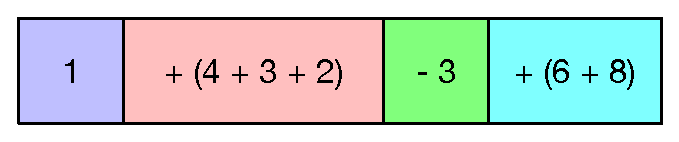
\includegraphics[width=0.35\linewidth]{images/basic_calculator_1}
	\caption{Basic Calculator I}
	\label{fig:basiccalculator1}
\end{figure}

\section{LC 0227 - Basic Calculator II}
Given a string {\colorbox{CodeBackground}{\lstinline|s|}} which represents an expression, evaluate this expression and return its value. \\

The integer division should truncate toward zero.\\

You may assume that the given expression is always valid. All intermediate results will be in the range of {\colorbox{CodeBackground}{\lstinline|[-2^31, 2^31 - 1]|}}.\\

Note: You are not allowed to use any built-in function which evaluates strings as mathematical expressions, such as {\colorbox{CodeBackground}{\lstinline|eval()|}}. \\

Constraints:
\begin{itemize}
	\item {\colorbox{CodeBackground}{\lstinline|1 <= s.length <= 3 * 10^5|}}
	\item {\colorbox{CodeBackground}{\lstinline|s|}} consists of integers and operators ({\colorbox{CodeBackground}{\lstinline|+|}}, {\colorbox{CodeBackground}{\lstinline|-|}}, {\colorbox{CodeBackground}{\lstinline|*|}}, {\colorbox{CodeBackground}{\lstinline|/|}}) separated by some number of spaces.
	\item {\colorbox{CodeBackground}{\lstinline|s|}} represents a valid expression.
	\item All the integers in the expression are non-negative integers in the range {\colorbox{CodeBackground}{\lstinline|[0, 2^31 - 1]|}}.
	\item The answer is guaranteed to fit in a 32-bit integer.
\end{itemize}

Examples:
\begin{itemize}
	\item {\colorbox{CodeBackground}{\lstinline|"3+2*2"\ \ --> 7|}}
	\item {\colorbox{CodeBackground}{\lstinline|" 3/2 "\ \ --> 1|}}
	\item {\colorbox{CodeBackground}{\lstinline|" 3+5 / 2 "\ \ --> 5|}}
\end{itemize}


\subsection*{Solution}
\begin{lstlisting}
#include <stack>
#include <string>

int calculate(std::string s) {
	std::stack<int> stk;
	long long currentNumber = 0;
	char operation = '+';
	for (int i = 0; i < s.length(); i++) {
		char currentChar = s[i];
		if (isdigit(currentChar)) { currentNumber = (currentNumber * 10) + (currentChar - '0'); }
		if (!isdigit(currentChar) && !isspace(currentChar) || i == s.length() - 1) {
			if (operation == '-') {
				stk.push(-currentNumber);
			} else if (operation == '+') {
				stk.push(currentNumber);
			} else if (operation == '*') {
				int stackTop = stk.top();
				stk.pop();
				stk.push(stackTop * currentNumber);
			} else if (operation == '/') {
				int stackTop = stk.top();
				stk.pop();
				stk.push(stackTop / currentNumber);
			}
			operation = currentChar;  // save the current operation
			currentNumber = 0;        // reset number for next iteration
		}
	}
	int result = 0;
	while (!stk.empty()) {
		result += stk.top();
		stk.pop();
	}
	return result;
}
\end{lstlisting}

\chapter{Monotonic Stack}

\section{LC 0739 - Daily Temperatures}
Given an array of integers {\colorbox{CodeBackground}{\lstinline|temperatures|}} represents the daily temperatures, return an array {\colorbox{CodeBackground}{\lstinline|answer|}} such that {\colorbox{CodeBackground}{\lstinline|answer[i]|}} is the number of days you have to wait after the {\colorbox{CodeBackground}{\lstinline|i|}}th day to get a warmer temperature. If there is no future day for which this is possible, keep {\colorbox{CodeBackground}{\lstinline|answer[i] == 0|}} instead.\\

Examples:
\begin{itemize}
\item {\colorbox{CodeBackground}{\lstinline|temperatures = [73,74,75,71,69,72,76,73] --> [1,1,4,2,1,1,0,0]|}}
\item {\colorbox{CodeBackground}{\lstinline|temperatures = [30,40,50,60] --> [1,1,1,0]|}}
\item {\colorbox{CodeBackground}{\lstinline|temperatures = [30,60,90] --> [1,1,0]|}}
\end{itemize}

\subsection*{Solution - Monotonic Stack}
\begin{lstlisting}
std::vector<int> dailyTemperatures(std::vector<int>& temperatures) {
  std::vector<int> num_days(temperatures.size(), 0);
  std::stack<int> stk;
  for (int i = 0; i < temperatures.size(); ++i) {
    while (!stk.empty() && temperatures[i] > temperatures[stk.top()]) {
      int top = stk.top();
      stk.pop();
      num_days[top] = i - top;
    }
    stk.push(i);
  }
  return num_days;
}
\end{lstlisting}

\section{LC 0496 - Next Greater Element I}
You are given two {\colorbox{CodeBackground}{\lstinline|0|}}-indexed integer arrays {\colorbox{CodeBackground}{\lstinline|nums1|}} and {\colorbox{CodeBackground}{\lstinline|nums2|}} \ul{without duplicates}, where {\colorbox{CodeBackground}{\lstinline|nums1|}} is a subset of {\colorbox{CodeBackground}{\lstinline|nums2|}}. \\

 For every integer in {\colorbox{CodeBackground}{\lstinline|nums1|}}, return the \ul{next greater number} in {\colorbox{CodeBackground}{\lstinline|nums2|}}. If there is no such \ul{next greater element} in {\colorbox{CodeBackground}{\lstinline|nums2|}}, return {\colorbox{CodeBackground}{\lstinline|-1.|}}.\\
 
 Explanation: For each {\colorbox{CodeBackground}{\lstinline|0 <= i < nums1.size()|}}, find the index {\colorbox{CodeBackground}{\lstinline|j|}} such that {\colorbox{CodeBackground}{\lstinline|nums1[i] == nums2[j]|}} and determine the \ul{next greater element} of {\colorbox{CodeBackground}{\lstinline|nums2[j]|}} in {\colorbox{CodeBackground}{\lstinline|nums2|}}. Return {\colorbox{CodeBackground}{\lstinline|-1|}} is there is no such \ul{next greater number} in {\colorbox{CodeBackground}{\lstinline|nums2|}}.\\

The \ul{next greater element} of some element {\colorbox{CodeBackground}{\lstinline|x|}} in an array is the first greater element that is to the right of {\colorbox{CodeBackground}{\lstinline|x|}} in the same array.\\

Examples:
\begin{itemize}
\item {\colorbox{CodeBackground}{\lstinline|nums1 = [4,1,2], nums2 = [1,3,4,2] --> [-1,3,-1]|}}\\
The next greater element for each value of {\colorbox{CodeBackground}{\lstinline|nums1|}} is as follows:\\
- {\colorbox{CodeBackground}{\lstinline|4|}} is underlined in $nums2 = [1,3,\underline{4},2]$ There is no next greater element, so the answer is {\colorbox{CodeBackground}{\lstinline|-1|}}.\\
- {\colorbox{CodeBackground}{\lstinline|1|}} is underlined in $nums2 = [\underline{1},3,4,2]$. The next greater element is {\colorbox{CodeBackground}{\lstinline|3|}}.\\
- {\colorbox{CodeBackground}{\lstinline|2|}} is underlined in $nums2 = [1,3,4,\underline{2}]$. There is no next greater element, so the answer is {\colorbox{CodeBackground}{\lstinline|-1|}}.
\item {\colorbox{CodeBackground}{\lstinline|nums1 = [2,4], nums2 = [1,2,3,4] --> [3,-1]|}}\\
The next greater element for each value of {\colorbox{CodeBackground}{\lstinline|nums1|}} is as follows:\\
- {\colorbox{CodeBackground}{\lstinline|2|}} is underlined in $nums2 = [1,\underline{2},3,4]$. The next greater element is {\colorbox{CodeBackground}{\lstinline|3|}}.\\
- {\colorbox{CodeBackground}{\lstinline|4|}} is underlined in $nums2 = [1,2,3,\underline{4}]$. There is no next greater element, so the answer is {\colorbox{CodeBackground}{\lstinline|-1|}}.
\end{itemize}

\subsection*{Solution - Monotonic Stack}
\begin{lstlisting}
std::vector<int> nextGreaterElement(std::vector<int>& nums1, std::vector<int>& nums2) {
  std::stack<int> stk;
  std::unordered_map<int, int> num2next_greater;
  for (int num : nums2) {
    while (!stk.empty() && num > stk.top()) {
      num2next_greater[stk.top()] = num;
      stk.pop();
    }
    stk.push(num);
  }
  std::vector<int> result;
  for (int num : nums1) {
    if (num2next_greater.find(num) != num2next_greater.end()) {
      result.push_back(num2next_greater[num]);
    } else {
      result.push_back(-1);
    }
  }
  return result;
}
\end{lstlisting}

\section{LC 0503 - Next Greater Element II}
Given a \ul{circular} integer array {\colorbox{CodeBackground}{\lstinline|nums|}} (i.e., the next element of {\colorbox{CodeBackground}{\lstinline|nums.back()|}} is {\colorbox{CodeBackground}{\lstinline|nums.front()|}}), return the \ul{next greater number} for every element in {\colorbox{CodeBackground}{\lstinline|nums|}}.\\

The \ul{next greater number} of a number {\colorbox{CodeBackground}{\lstinline|x|}} is the first greater number to its traversing-order next in the array, which means you could search circularly to find its next greater number. If it doesn't exist, return {\colorbox{CodeBackground}{\lstinline|-1|}} for this number.\\

Examples:
\begin{itemize}
\item {\colorbox{CodeBackground}{\lstinline|nums = [1,2,1] --> [2,-1,2]|}}\\
The first {\colorbox{CodeBackground}{\lstinline|1|}}'s next greater number is {\colorbox{CodeBackground}{\lstinline|2|}}. \\
The number {\colorbox{CodeBackground}{\lstinline|2|}} can't find next greater number. \\
The second {\colorbox{CodeBackground}{\lstinline|1|}}'s next greater number needs to search circularly, which is also {\colorbox{CodeBackground}{\lstinline|2|}}.
\item {\colorbox{CodeBackground}{\lstinline|nums = [1,2,3,4,3] --> [2,3,4,-1,4]|}}
\end{itemize}

\subsection*{Solution - Monotonic Stack}
\begin{lstlisting}
std::vector<int> nextGreaterElements(std::vector<int>& nums) {
  int n = nums.size();
  std::vector<int> result(n, -1);
  std::stack<int> stk;
  for (int i = 0; i < n * 2; ++i) {
    int num = nums[i % n];
    while (!stk.empty() && num > nums[stk.top()]) {
      result[stk.top()] = num;
      stk.pop();
    }
    if (i < n) { stk.push(i); }
  }
  return result;
}
\end{lstlisting}

\section{LC 0042 - Trapping Rain Water}
Given {\colorbox{CodeBackground}{\lstinline|n|}} ({\colorbox{CodeBackground}{\lstinline|n >= 1|}}) non-negative integers representing an elevation map where the width of each bar is {\colorbox{CodeBackground}{\lstinline|1|}}, compute how much water it can trap after raining.\\

Example: {\colorbox{CodeBackground}{\lstinline|height = [0,1,0,2,1,0,1,3,2,1,2,1] --> 6|}}
\begin{figure}[H]
\centering
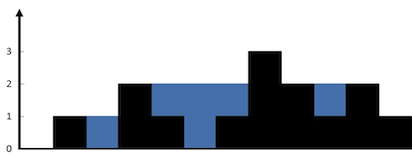
\includegraphics[width=0.4\linewidth]{images/lc0042_eg}
\end{figure}

\subsection*{Solution - Monotonic Stack}\label{solution:lc0042_monotonic_stack}
\begin{lstlisting}
int trap(std::vector<int>& heights) {
  std::stack<int> stk;
  int trapped_water = 0;
  int i = 0;
  while (i < heights.size()) {
    while (!stk.empty() && heights[i] > heights[stk.top()]) {
      int top = stk.top();
      stk.pop();
      if (stk.empty()) { break; }
      int width = i - stk.top() - 1;
      int height = std::min(heights[i], heights[stk.top()]) - heights[top];
      trapped_water += width * height;
    }
    stk.push(i);
    ++i;
  }
  return trapped_water;
}
\end{lstlisting}

\subsection*{Other Solutions}
\begin{itemize}
\item \hyperref[solution:lc0042_brute_force]{Brute Force (Time Limit Exceeded)}
\item \hyperref[solution:lc0042_brute_force_optimized_1]{Brute Force, Optimized 1}
\item \hyperref[solution:lc0042_brute_force_optimized_2]{Brute Force, Optimized 2}
%\item \hyperref[solution:lc0042_monotonic_stack]{Monotonic Stack}
\end{itemize}

\section{LC 0084 - Largest Rectangle in Histogram}
Given an array of integers {\colorbox{CodeBackground}{\lstinline|heights|}} representing the histogram's bar height where the width of each bar is {\colorbox{CodeBackground}{\lstinline|1|}}, return the area of the largest rectangle in the histogram.

\begin{itemize}
\item Example 1: {\colorbox{CodeBackground}{\lstinline|heights = [2,1,5,6,2,3] --> 10|}}
\begin{figure}[H]
\centering
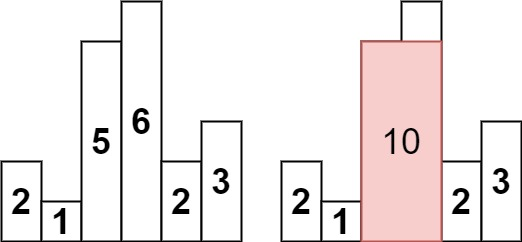
\includegraphics[width=0.3\linewidth]{images/lc0084_eg1}
\label{fig:lc0084eg1}
\end{figure}
\item Example 2: {\colorbox{CodeBackground}{\lstinline|heights = [2,4] --> 4|}}
\begin{figure}[H]
\centering
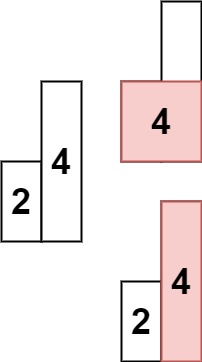
\includegraphics[width=0.11\linewidth]{images/lc0084_eg2}
\label{fig:lc0084eg2}
\end{figure}
\end{itemize}

\subsection*{Solution - Monotonic Stack}
\begin{lstlisting}
int largestRectangleArea(std::vector<int>& heights) {
  std::stack<int> s;
  int max_area = 0;
  for (int i = 0; i <= heights.size(); ++i) {
    int h = (i == heights.size() ? 0 : heights[i]);
    if (s.empty() || h >= heights[s.top()]) {
      s.push(i);
    } else {
      int tp = s.top();
      s.pop();
      int width = s.empty() ? i : i - s.top() - 1;
      max_area = std::max(max_area, heights[tp] * width);
      i--;
    }
  }
  return max_area;
}
\end{lstlisting}
\chapter{Queue}
\section{LC 0232 - Implement Queue using Stacks}
Implement a \ul{first in first out (FIFO) queue} using only \ul{two stacks}.\\

Implement the {\colorbox{CodeBackground}{\lstinline|MyQueue|}} class:
\begin{itemize}
\item {\colorbox{CodeBackground}{\lstinline|void push(int x)|}} - Pushes element x to the back of the queue.
\item {\colorbox{CodeBackground}{\lstinline|int pop()|}} - Removes the element from the front of the queue and returns it.
\item{\colorbox{CodeBackground}{\lstinline| int peek()|}} ({\colorbox{CodeBackground}{\lstinline|std::queue::front()|}}) - Returns the element at the front of the queue.
\item {\colorbox{CodeBackground}{\lstinline|bool empty()|}} - Returns {\colorbox{CodeBackground}{\lstinline|true|}} if the queue is empty, {\colorbox{CodeBackground}{\lstinline|false|}} otherwise.
\end{itemize}

\subsection*{Solution}
\begin{lstlisting}
class MyQueue {
 public:
  MyQueue() {}

  void push(int x) { in_stk.push(x); }

  int pop() {
    if (out_stk.empty()) { transfer(); }
    int front = out_stk.top();
    out_stk.pop();
    return front;
  }

  int peek() {  // std::queue::front()
    if (out_stk.empty()) { transfer(); }
    return out_stk.top();
  }

  bool empty() { return in_stk.empty() && out_stk.empty(); }

 private:
  std::stack<int> in_stk;
  std::stack<int> out_stk;

  // transfer elements from in_stk to out_stk
  void transfer() {
    while (!in_stk.empty()) {
      out_stk.push(in_stk.top());
      in_stk.pop();
    }
  }
};
\end{lstlisting}

\section{LC 0225 - Implement Stack using Queues}
Implement a \ul{last-in-first-out (LIFO) stack} using only \ul{two queues}.\\

Implement the {\colorbox{CodeBackground}{\lstinline|MyStack|}} class:
\begin{itemize}
\item {\colorbox{CodeBackground}{\lstinline|void push(int x)|}} - Pushes element {\colorbox{CodeBackground}{\lstinline|x|}} to the top of the stack.
\item {\colorbox{CodeBackground}{\lstinline|int pop()|}} - Removes the element on the top of the stack and returns it.
\item {\colorbox{CodeBackground}{\lstinline|int top()|}} - Returns the element on the top of the stack.
\item {\colorbox{CodeBackground}{\lstinline|bool empty()|}} - Returns {\colorbox{CodeBackground}{\lstinline|true|}} if the stack is empty, {\colorbox{CodeBackground}{\lstinline|false|}} otherwise.
\end{itemize}

\subsection*{Solution 1 - Two Queues}
\begin{lstlisting}
class MyStack {
 public:
  MyStack() {}

  void push(int x) {
    q2.push(x);
    while (!q1.empty()) {
      q2.push(q1.front());
      q1.pop();
    }
    std::swap(q1, q2);
  }

  int pop() {
    if (q1.empty()) { return -1; }
    int top = q1.front();
    q1.pop();
    return top;
  }

  int top() {
    if (q1.empty()) { return -1; }
    return q1.front();
  }

  bool empty() { return q1.empty(); }

 private:
  std::queue<int> q1;
  std::queue<int> q2;
};
\end{lstlisting}

\subsection*{Solution 2 - One Queue}
\begin{lstlisting}
class MyStack {
 public:
  void push(int x) {
    q.push(x);
    for (int i = 0; i < q.size() - 1; ++i) {
      q.push(q.front());
      q.pop();
    }
  }

  int pop() {
    int top = q.front();
    q.pop();
    return top;
  }

  int top() { return q.front(); }

  bool empty() { return q.empty(); }

 private:
  std::queue<int> q;
};
\end{lstlisting}

\chapter{Priority Queue}
\section{LC 0347 - Top K Frequent Elements}
Given a \ul{non-empty} integer array {\colorbox{CodeBackground}{\lstinline|nums|}} and an integer {\colorbox{CodeBackground}{\lstinline|k|}} ({\colorbox{CodeBackground}{\lstinline|k >= 1|}}), return the {\colorbox{CodeBackground}{\lstinline|k|}} most frequent elements. You may return the answer in any order.\\

Examples:
\begin{itemize}
\item {\colorbox{CodeBackground}{\lstinline|nums = [1,1,1,2,2,3], k = 2 --> [1,2]|}}
\item {\colorbox{CodeBackground}{\lstinline|nums = [1], k = 1 --> [1]|}}
\end{itemize}

\subsection*{Solution - Priority Queue}
\begin{lstlisting}
std::vector<int> topKFrequent(std::vector<int>& nums, int k) {
  std::unordered_map<int, int> num2freq;
  for (int num : nums) { num2freq[num]++; }
  auto comp = [&num2freq](int n1, int n2) { return num2freq[n1] > num2freq[n2]; };
  std::priority_queue<int, std::vector<int>, decltype(comp)> heap(comp);
  for (auto& [num, freq] : num2freq) {
    heap.push(num);
    if (heap.size() > k) { heap.pop(); }
  }
  std::vector<int> top_k;
  while (!heap.empty()) {
    top_k.push_back(heap.top());
    heap.pop();
  }
  return top_k;
}
\end{lstlisting}

\section{LC 0148 - Sort List}
Given the {\colorbox{CodeBackground}{\lstinline|head|}} of a \ul{singly linked list}, return the list after sorting it in ascending order.\\

Examples:
\begin{itemize}
\item {\colorbox{CodeBackground}{\lstinline|[4 -> 2 -> 1 -> 3] --> [1 -> 2 -> 3 -> 4]|}}
\item {\colorbox{CodeBackground}{\lstinline|[-1 -> 5 -> 3 -> 4 -> 0] --> [-1 -> 0 -> 3 -> 4 -> 5]|}}
\item {\colorbox{CodeBackground}{\lstinline|[] --> []|}}
\end{itemize}

\subsection*{Solution - Priority Queue}\label{solution:lc-148_priority_queue}
\begin{lstlisting}
ListNode* sortList(ListNode* head) {
  if (!head) { return nullptr; }
  auto compare = [](const ListNode* lhs, const ListNode* rhs) {
    return lhs->val > rhs->val;
  };
  std::priority_queue<ListNode*, std::vector<ListNode*>, decltype(compare)> min_heap(
      compare);
  while (head) {
    min_heap.push(head);
    head = head->next;
  }
  ListNode* dummy_head = new ListNode();
  ListNode* curr = dummy_head;
  while (!min_heap.empty()) {
    curr->next = min_heap.top();
    min_heap.pop();
    curr = curr->next;
  }
  curr->next = nullptr;
  return dummy_head->next;
}
\end{lstlisting}

\subsection*{Other Solutions}
\begin{itemize}
\item \hyperref[solution:lc0148_merge_sort]{Merge Sort}
%\item \hyperref[solution:lc-148_priority_queue]{Priority Queue}
\end{itemize}
\chapter{Tree}
\section{Thinking in General Trees}
{\color{blue}{Tree}} data structures usually have specific application scenarios. Unlike {\color{blue}{arrays}}, {\color{blue}{lists}}, and {\color{blue}{graphs}}, which can be seen everywhere in daily life, trees are {\color{blue}{more abstract}}. You need to get familiar with those scenarios and the corresponding solutions.

\subsection{Trees and Recursion}
{\color{ForestGreen}{Recursive algorithms are usually a natural fit for tree-based problems!}}\\
{[Reason]} Trees are {\color{blue}{hierarchical data structures}} with a {\color{blue}{parent-child relationship}}. Each {\color{blue}{subtree}} can be viewed as a {\color{blue}{tree}} itself. This mirrors the concept of {\color{blue}{recursion}} where a problem is solved by solving smaller instances of the same problem. In addition, in many problems, {\color{blue}{\ul{children of leaf nodes} or \ul{leaf nodes} are natural \ul{base cases}}}, which makes recursive algorithms easier to design.\\

Practical Tips: 
\begin{itemize}
	\item {\color{blue}{If a tree-based problem can be tackled by iteratively addressing smaller sub-problems from the root down to the leaf nodes, recursive algorithm is often a good choice.}}
	\item {\color{blue}{It's often more practical to use the \ul{children of leaf nodes} as {\color{blue}{\ul{base cases}}} instead of the leaf nodes themselves, as it's much easier to identify if a node is a child of a leaf node.}}
\end{itemize}

\subsection{Tree v.s. Graph}
A tree is a {\color{blue}{connected acyclic undirected graph}}, so in some scenarios we can consider trees in the same way as graphs. \\

For example:
\begin{itemize}
	\item {\color{blue}{Level-order traversal in trees}} is {\color{blue}{BFS in graphs}}, where the traversal begins from the root node.
	\item {\color{blue}{Pre-order traversal in trees}} is analogous to {\color{blue}{DFS in graphs}}, starting from the root and exploring the left subtree first, followed by the right subtree.
\end{itemize}

\section{Thinking in Binary Trees}
A {\color{blue}{binary tree}} is a type of tree where each node can have \ul{maximum of two children}.\\

\hdashrule[0.5ex]{\linewidth}{0.5pt}{1mm 3pt}
Unless specified, {\color{blue}{nodes}} of {\color{blue}{binary trees}} are defined as follows:
\begin{lstlisting}
struct TreeNode {
	TreeNode() : val(0), left(nullptr), right(nullptr) {}
	TreeNode(int x) : val(x), left(nullptr), right(nullptr) {}
	TreeNode(int x, TreeNode* left, TreeNode* right) : val(x), left(left), right(right) {}
	
	int val;
	TreeNode *left;
	TreeNode *right;
};
\end{lstlisting}
\hdashrule[0.5ex]{\linewidth}{0.5pt}{1mm 3pt}

\section{Thinking in Complete Binary Tree}

\section{Thinking in Balanced Binary Tree}

\section{Thinking in Binary Search Trees (BST)}
A {\color{blue}{binary search tree (BST)}} is a {\color{blue}{binary tree}} where each node has a value greater than all values in its {\color{blue}{left subtree}} and less than or equal to all values in its {\color{blue}{right subtree}}. \\

{\color{blue}{In-order traversal}} of a BST visits the nodes in a {\color{blue}{non-decreasing order}} of their values.


\section{LC 0104 - Maximum Depth of Binary Tree}
Given the root of a \ul{binary tree}, return its \ul{maximum depth}.

\subsection*{Solution - Recursion}
In this solution, we use {\color{blue}{children of leaf nodes}} as the {\color{blue}{base cases}}.
\begin{lstlisting}
int maxDepth(TreeNode* root) {
	// base case: child of leaf node
	if (!root) { return 0; }
	return std::max(maxDepth(root->left), maxDepth(root->right)) + 1;
}
\end{lstlisting}

\subsection*{*Solution - Recursion}
In this solution, we use {\color{blue}{children of leaf nodes}} and {\color{blue}{leaf nodes}} as the {\color{blue}{base cases}}.
\begin{lstlisting}
int maxDepth(TreeNode* root) {
	// base case: child of leaf node
	if (!root) { return 0; }
	// base case: leaf node
	if (!root->left && !root->right) { return 1; }
	return std::max(maxDepth(root->left), maxDepth(root->right)) + 1;
}
\end{lstlisting}

\section{LC 0111 - Minimum Depth of Binary Tree}
Given a \ul{binary tree}, find its \ul{minimum depth}.

\subsection*{Solution - Recursion}
\begin{lstlisting}
int minDepth(TreeNode* root) {
  if (!root) { return 0; }
  if (!root->left && !root->right) { return 1; }
  if (root->left && root->right) {
    return 1 + std::min(minDepth(root->left), minDepth(root->right));
  }
  if (!root->left) { return 1 + minDepth(root->right); }
  if (!root->right) { return 1 + minDepth(root->left); }
  return -1;
}
\end{lstlisting}

\subsection*{Solution 2 - Level-order Traversal}
\begin{lstlisting}
int minDepth(TreeNode* root) {
  if (!root) { return 0; }
  std::queue<std::pair<TreeNode*, int>> q;
  q.push({root, 1});
  while (!q.empty()) {
    auto [node, depth] = q.front();
    q.pop();
    if (!node->left && !node->right) { return depth; }
    if (node->left) { q.push({node->left, depth + 1}); }
    if (node->right) { q.push({node->right, depth + 1}); }
  }
  return -1;
}
\end{lstlisting}

\section{LC 0100 - Same Tree}
Given the roots of two \ul{binary trees} {\colorbox{CodeBackground}{\lstinline|p|}} and {\colorbox{CodeBackground}{\lstinline|q|}}, write a function to check if they are the same or not.\\

Two binary trees are considered the same if they are structurally identical, and the nodes have the same value.

\subsection*{Solution - Recursion}
\begin{lstlisting}
bool isSameTree(TreeNode* p, TreeNode* q) {
  // base case 1: both nodes are children of leaf nodes
  if (!p && !q) { return true; }
  // base case 2: one node is child of leaf node and the other is not
  if (!p || !q) { return false; }
  return (p->val == q->val) && isSameTree(p->left, q->left)
         && isSameTree(p->right, q->right);
}
\end{lstlisting}

\section{LC 0101 - Symmetric Tree}
Given the {\colorbox{CodeBackground}{\lstinline|root|}} of a \ul{binary tree}, check whether it is a mirror of itself (i.e., symmetric around its center).\\

A symmetric tree:
\begin{figure}[H]
	\centering
	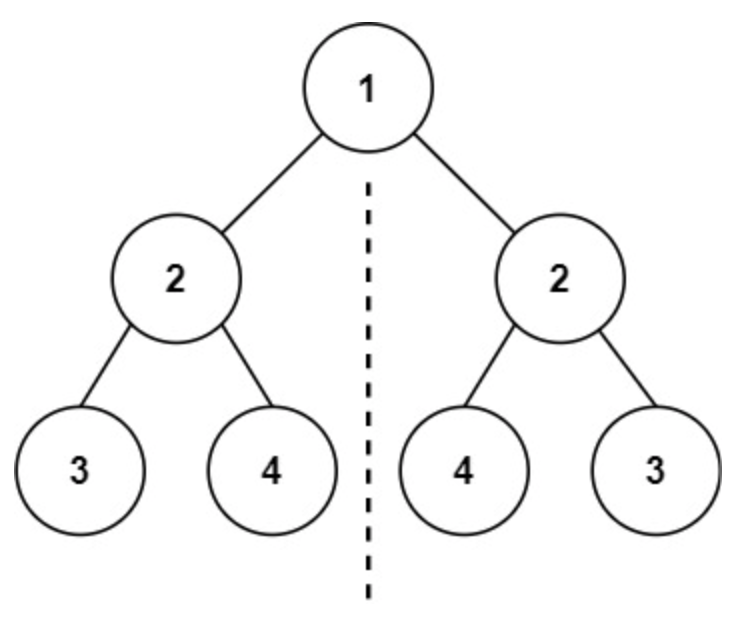
\includegraphics[width=0.25\linewidth]{images/lc0101_example}
	\label{fig:lc0101example}
\end{figure}

\subsection*{Solution - Recursion}
\begin{lstlisting}
bool isSymmetric(TreeNode* root) {
	if (!root) { return true; }
	return isSymmetricRecursive(root->left, root->right);
}

bool isSymmetricRecursive(TreeNode* t1, TreeNode* t2) {
  // base case 1: both nodes are children of leaf nodes
  if (!t1 && !t2) { return true; }
  // base case 2: one node is child of leaf node and the other is not
  if (!t1 || !t2) { return false; }
  return t1->val == t2->val && isSymmetricRecursive(t1->left, t2->right)
         && isSymmetricRecursive(t1->right, t2->left);
}
\end{lstlisting}

\section{LC 0226 - Invert Binary Tree}
Given the {\colorbox{CodeBackground}{\lstinline|root|}} of a \ul{binary tree}, invert the tree, and return its root.\\

For example:
\begin{figure}[H]
	\centering
	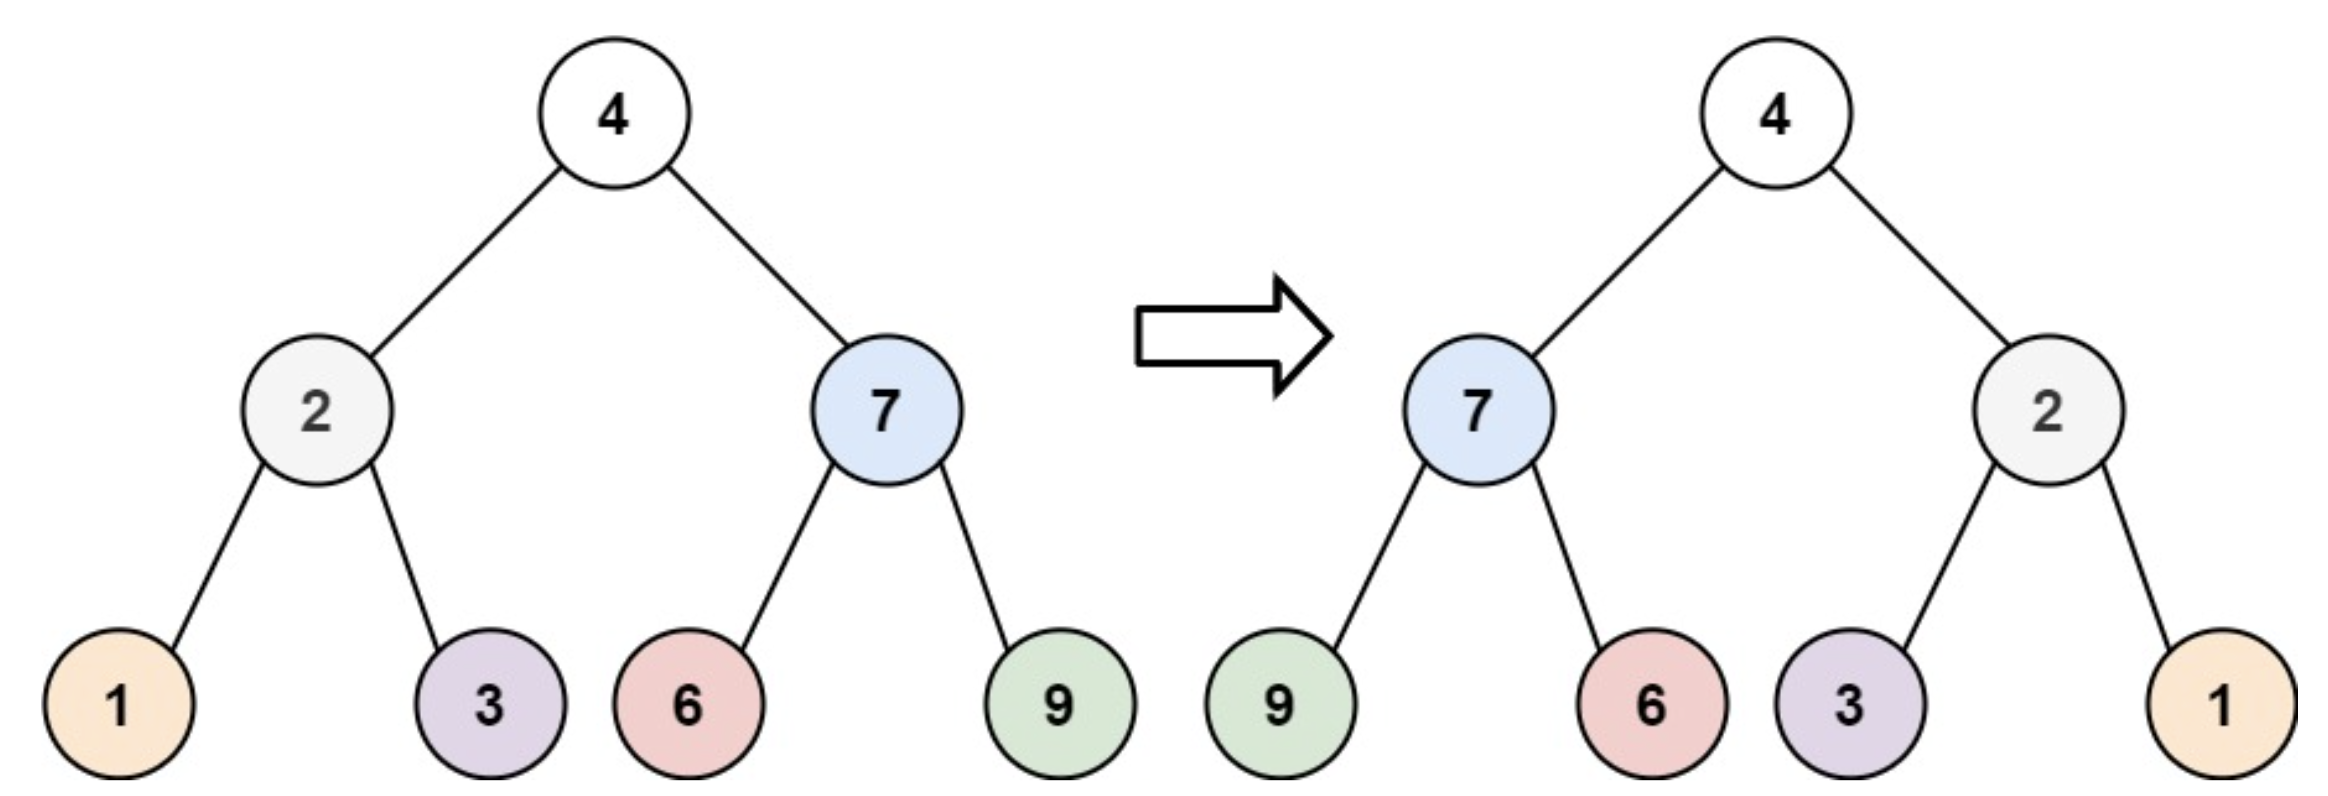
\includegraphics[width=0.7\linewidth]{images/lc0226_example}
	\label{fig:lc0226example}
\end{figure}

\subsection*{Solution - Recursion}
\begin{lstlisting}
	TreeNode* invertTree(TreeNode* root) {
		// base case: child of leaf node
		if (!root) { return root; }
		std::swap(root->left, root->right);
		invertTree(root->left);
		invertTree(root->right);
		return root;
	}
\end{lstlisting}

\section{LC 0236 - Lowest Common Ancestor of a Binary Tree}\label{lc0236}
Given a \ul{binary tree}, find the \ul{lowest common ancestor (LCA)} of two given nodes in the tree. Note that both {\colorbox{CodeBackground}{\lstinline|p|}} and {\colorbox{CodeBackground}{\lstinline|q|}} are in the tree and {\colorbox{CodeBackground}{\lstinline|p != q|}}.\\

Definition of LCA: The \ul{lowest common ancestor (LCA)} is defined between two nodes {\colorbox{CodeBackground}{\lstinline|p|}} and {\colorbox{CodeBackground}{\lstinline|q|}} as the lowest node in the tree that has both {\colorbox{CodeBackground}{\lstinline|p|}} and {\colorbox{CodeBackground}{\lstinline|q|}} as {\color{blue}{descendants}} (where we allow a node to be a {\color{blue}{descendant}} of itself). \\

Examples:
\begin{figure}[H]
	\centering
	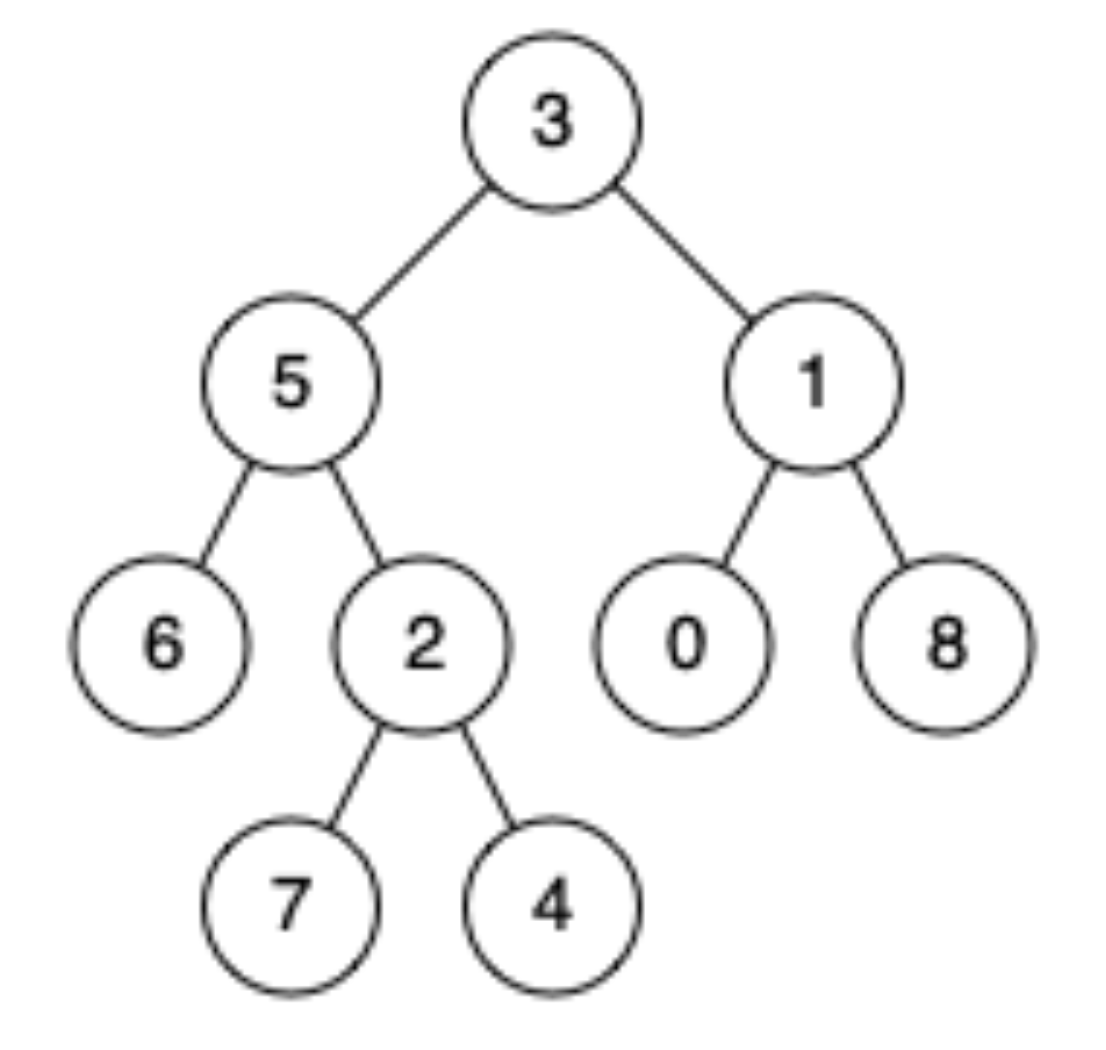
\includegraphics[width=0.3\linewidth]{images/lc0236_example_1}
	\label{fig:lc0236example1}
\end{figure}
\begin{itemize}
	\item {\colorbox{CodeBackground}{\lstinline|p = 5, q = 1 --> 3|}}
	\item {\colorbox{CodeBackground}{\lstinline|p = 5, q = 4 --> 5|}}
\end{itemize}

\subsection*{Solution - Add Parent Information}
\begin{lstlisting}
void CreateNode2Parent(TreeNode* root,
                       std::unordered_map<TreeNode*, TreeNode*>& node2parent) {
  if (!root) { return; }
  if (root->left) { node2parent[root->left] = root; }
  if (root->right) { node2parent[root->right] = root; }
  CreateNode2Parent(root->right, node2parent);
  CreateNode2Parent(root->left, node2parent);
}

TreeNode* lowestCommonAncestor(TreeNode* root, TreeNode* p, TreeNode* q) {
  if (!root) { return nullptr; }
  std::unordered_map<TreeNode*, TreeNode*> node2parent;
  node2parent[root] = nullptr;
  CreateNode2Parent(root, node2parent);
  std::vector<TreeNode*> path_p;
  while (p) {
    path_p.push_back(p);
    p = node2parent[p];
  }
  std::reverse(path_p.begin(), path_p.end());
  std::vector<TreeNode*> path_q;
  while (q) {
    path_q.push_back(q);
    q = node2parent[q];
  }
  std::reverse(path_q.begin(), path_q.end());
  TreeNode* lca = nullptr;
  int i = 0;
  while (i < std::min(path_p.size(), path_q.size()) && path_p[i] == path_q[i]) {
    lca = path_p[i];
    ++i;
  }
  return lca;
}
\end{lstlisting}

\subsection*{Solution - Recursion}
\begin{lstlisting}
// 1. both p and q are in the tree --> LCA
// 2. only one of p and q is in the tree --> that one
// 3. neither p nor q is in the tree --> nullptr
TreeNode* lowestCommonAncestor(TreeNode* root, TreeNode* p, TreeNode* q) {
	if (!root) { return nullptr; }
	if (root == p || root == q) { return root; }
	// search for LCA in left and right subtrees
	TreeNode* left = lowestCommonAncestor(root->left, p, q);
	TreeNode* right = lowestCommonAncestor(root->right, p, q);
	// if p and q are in different subtrees, return root
	if (left && right) { return root; }
	// o.w., return subtree that contains p or q
	return left ? left : right;
}
\end{lstlisting}

\subsection*{Related}
\begin{itemize}
	\item \hyperref[lc0236]{LC 0236 - Lowest Common Ancestor of a Binary Tree}
	\item \hyperref[lc0235]{LC 0235 - Lowest Common Ancestor of a BST}
\end{itemize}

\section{LC 0144 - Binary Tree Pre-order Traversal}
Given the {\colorbox{CodeBackground}{\lstinline|root|}} of a \ul{binary tree}, return the {\color{blue}{pre-order traversal}} of its nodes' values.

\subsection*{Solution - Recursion}
\begin{lstlisting}
std::vector<int> preorderTraversal(TreeNode* root) {
	static std::vector<int> res = {};
	if (!root) { return res; }
	res.push_back(root->val);
	preorderTraversal(root->left);
	preorderTraversal(root->right);
	return res;
}
\end{lstlisting}

\subsection*{Solution - Iterative}
\begin{lstlisting}
std::vector<int> preorderTraversal(TreeNode* root) {
  std::vector<int> res = {};
  if (!root) { return res; }
  std::stack<TreeNode*> stk;
  stk.push(root);
  while (!stk.empty()) {
    TreeNode* top = stk.top();
    stk.pop();
    res.push_back(top->val);
    if (top->right) { stk.push(top->right); }
    if (top->left) { stk.push(top->left); }
  }
  return res;
}
\end{lstlisting}

\section{LC 0094 - Binary Tree In-order Traversal}
Given the {\colorbox{CodeBackground}{\lstinline|root|}} of a \ul{binary tree}, return the {\color{blue}{in-order traversal}} of its nodes' values.

\subsection*{Solution - Recursion}
\begin{lstlisting}
std::vector<int> inorderTraversal(TreeNode* root) {
	static std::vector<int> res = {};
	if (!root) { return res; }
	inorderTraversal(root->left);
	res.push_back(root->val);
	inorderTraversal(root->right);
	return res;
}
\end{lstlisting}

\subsection*{Solution - Iterative}
\begin{lstlisting}
std::vector<int> inorderTraversal(TreeNode* root) {
	std::vector<int> res = {};
	if (!root) { return res; }
	std::stack<TreeNode*> stk;
	TreeNode* curr = root;
	while (curr || !stk.empty()) {
		while (curr) {
			stk.push(curr);
			curr = curr->left;
		}
		TreeNode* top = stk.top();
		stk.pop();
		res.push_back(top->val);
		curr = top->right;
	}
	return res;
}
\end{lstlisting}

\section{LC 0145 - Binary Tree Post-order Traversal}
Given the {\colorbox{CodeBackground}{\lstinline|root|}} of a \ul{binary tree}, return the {\color{blue}{post-order traversal}} of its nodes' values.

\subsection*{Solution - Recursion}
\begin{lstlisting}
std::vector<int> postorderTraversal(TreeNode* root) {
	static std::vector<int> res = {};
	if (!root) { return res; }
	postorderTraversal(root->left);
	postorderTraversal(root->right);
	res.push_back(root->val);
	return res;
}
\end{lstlisting}

\subsection*{Solution - Iterative}
\begin{lstlisting}
std::vector<int> postorderTraversal(TreeNode* root) {
	std::vector<int> res = {};
	if (!root) { return res; }
	std::stack<TreeNode*> stk;
	TreeNode* curr = root;
	TreeNode* last_visit = nullptr;
	while (curr || !stk.empty()) {
		while (curr) {
			stk.push(curr);
			curr = curr->left;
		}
		TreeNode* top = stk.top();
		if (top->right && top->right != last_visit) {
			// right node exists && right node is not visited
			curr = top->right;
		} else {
			// right node does not exist || right node is visited
			// handle the node, e.g., print it
			res.push_back(top->val);
			last_visit = top;
			stk.pop();
		}
	}
	return res;
}
\end{lstlisting}

\section{LC 0105 - Construct Binary Tree from Pre-order and In-order Traversal}
Given two integer arrays {\colorbox{CodeBackground}{\lstinline|preorder|}} and {\colorbox{CodeBackground}{\lstinline|inorder|}} where {\colorbox{CodeBackground}{\lstinline|preorder|}} is the \ul{pre-order traversal} of a \ul{binary tree} and {\colorbox{CodeBackground}{\lstinline|inorder|}} is the \ul{in-order traversal} of the same tree, construct and return the binary tree. It should be noted that {\colorbox{CodeBackground}{\lstinline|preorder|}} and {\colorbox{CodeBackground}{\lstinline|inorder|}} consist of unique values. \\

Example:
\begin{figure}[H]
	\centering
	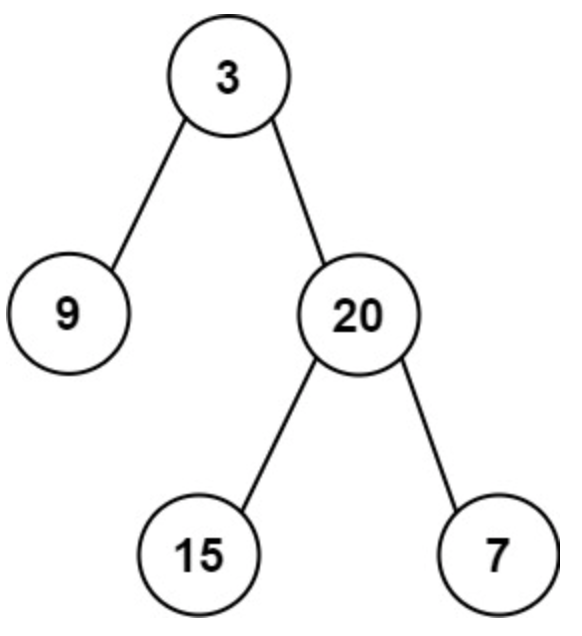
\includegraphics[width=0.23\linewidth]{images/lc0105_example}
	\label{fig:lc0105example}
\end{figure}
{\colorbox{CodeBackground}{\lstinline|preorder = [3,9,20,15,7], inorder = [9,3,15,20,7] --> [3,9,20,nullptr,nullptr,15,7]|}}

\subsection*{Solution}
The steps are as follows:
\begin{enumerate}
	\item Use the {\color{blue}{first element}} of the {\colorbox{CodeBackground}{\lstinline|preorder|}} array to identify the {\color{blue}{root}}.
	\item Find this root in the {\colorbox{CodeBackground}{\lstinline|inorder|}} array. Elements to the left are part of the {\color{blue}{left subtree}}, and elements to the right are part of the {\color{blue}{right subtree}}.
	\item Recursively apply this logic to build the left and right subtrees.
\end{enumerate}
\begin{lstlisting}
TreeNode* buildTree(std::vector<int>& preorder, std::vector<int>& inorder) {
	std::unordered_map<int, int> in_val2idx;
	for (int i = 0; i < inorder.size(); i++) { in_val2idx[inorder[i]] = i; }
	return buildTreeRecursive(preorder, 0, preorder.size() - 1, inorder, 0, inorder.size() - 1,
	in_val2idx);
}

TreeNode* buildTreeRecursive(std::vector<int>& preorder, int pre_start, int pre_end,
std::vector<int>& inorder, int in_start, int in_end,
std::unordered_map<int, int>& in_val2idx) {
	// base case
	if (pre_start > pre_end || in_start > in_end) { return nullptr; }
	TreeNode* root = new TreeNode(preorder[pre_start]);
	int in_root = in_val2idx[root->val];
	int num_left = in_root - in_start;
	root->left = buildTreeRecursive(preorder, pre_start + 1, pre_start + num_left, inorder, 
	in_start, in_root - 1, in_val2idx);
	root->right = buildTreeRecursive(preorder, pre_start + num_left + 1, pre_end, 
	inorder, in_root + 1, in_end, in_val2idx);
	
	return root;
}
\end{lstlisting}

\section{LC 0106 - Construct Binary Tree from In-order and Post-order Traversal}
Given two integer arrays {\colorbox{CodeBackground}{\lstinline|inorder|}} and {\colorbox{CodeBackground}{\lstinline|postorder|}} where {\colorbox{CodeBackground}{\lstinline|inorder|}} is the \ul{in-order traversal} of a \ul{binary tree} and {\colorbox{CodeBackground}{\lstinline|postorder|}} is the \ul{post-order traversal} of the same tree, construct and return the binary tree. It should be noted that {\colorbox{CodeBackground}{\lstinline|inorder|}} and {\colorbox{CodeBackground}{\lstinline|postorder|}} consist of unique values.  \\

Example:
\begin{figure}[H]
	\centering
	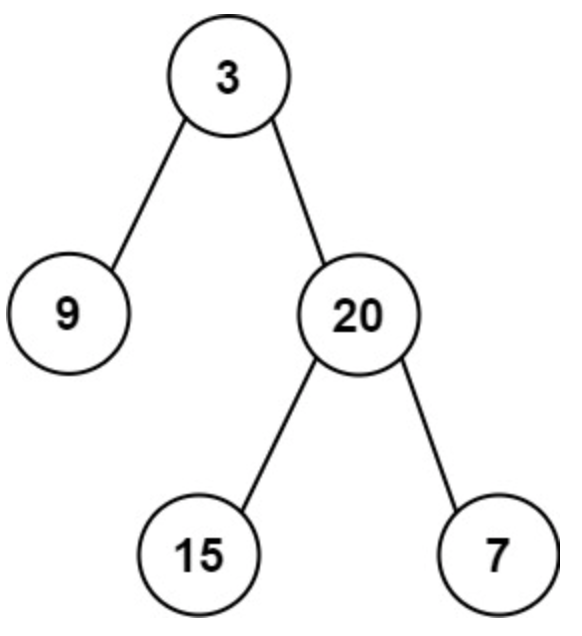
\includegraphics[width=0.23\linewidth]{images/lc0105_example}
	\label{fig:lc0106example}
\end{figure}
{\colorbox{CodeBackground}{\lstinline|inorder = [9,3,15,20,7], postorder = [9,15,7,20,3] --> [3,9,20,null,null,15,7]|}}

\subsection*{Solution}
The steps are as follows:
\begin{enumerate}
	\item Use the {\color{blue}{last element}} of the {\colorbox{CodeBackground}{\lstinline|postorder|}} array as the {\color{blue}{root}}.
	\item Find this root in the {\colorbox{CodeBackground}{\lstinline|inorder|}} array. Elements to the left are part of the {\color{blue}{left subtree}}, and elements to the right are part of the {\color{blue}{right subtree}}.
	\item Recursively apply this logic to build the left and right subtrees.
\end{enumerate}

\begin{lstlisting}
TreeNode* buildTree(std::vector<int>& inorder, std::vector<int>& postorder) {
	std::unordered_map<int, int> in_val2idx;
	for (int i = 0; i < inorder.size(); i++) { in_val2idx[inorder[i]] = i; }
	return buildTreeRecursive(inorder, 0, inorder.size() - 1, postorder, 0,
	postorder.size() - 1, in_val2idx);
}

TreeNode* buildTreeRecursive(std::vector<int>& inorder, int in_start, int in_end,
std::vector<int>& postorder, int post_start, int post_end,
std::unordered_map<int, int>& in_val2idx) {
	// base case
	if (in_start > in_end || post_start > post_end) { return nullptr; }
	TreeNode* root = new TreeNode(postorder[post_end]);
	int in_root = in_val2idx[root->val];
	int num_left = in_root - in_start;
	root->left = buildTreeRecursive(inorder, in_start, in_root - 1, postorder, post_start,
	post_start + num_left - 1, in_val2idx);
	root->right = buildTreeRecursive(inorder, in_root + 1, in_end, postorder, 
	post_start + num_left, post_end - 1, in_val2idx);
	return root;
}
\end{lstlisting}

\section{LC 0114 - Flatten Binary Tree to Linked List}
Given the {\colorbox{CodeBackground}{\lstinline|root|}} of a \ul{binary tree}, flatten the tree into a \ul{linked list}:
\begin{itemize}
	\item The linked list should use the same {\colorbox{CodeBackground}{\lstinline|TreeNode|}} class where the {\colorbox{CodeBackground}{\lstinline|right|}} child pointer points to the next node in the list and the left child pointer is always {\colorbox{CodeBackground}{\lstinline|nullptr|}}.
	\item The linked list should be in the same order as a \ul{pre-order traversal} of the binary tree.
\end{itemize}

Example:

\begin{figure}[H]
	\centering
	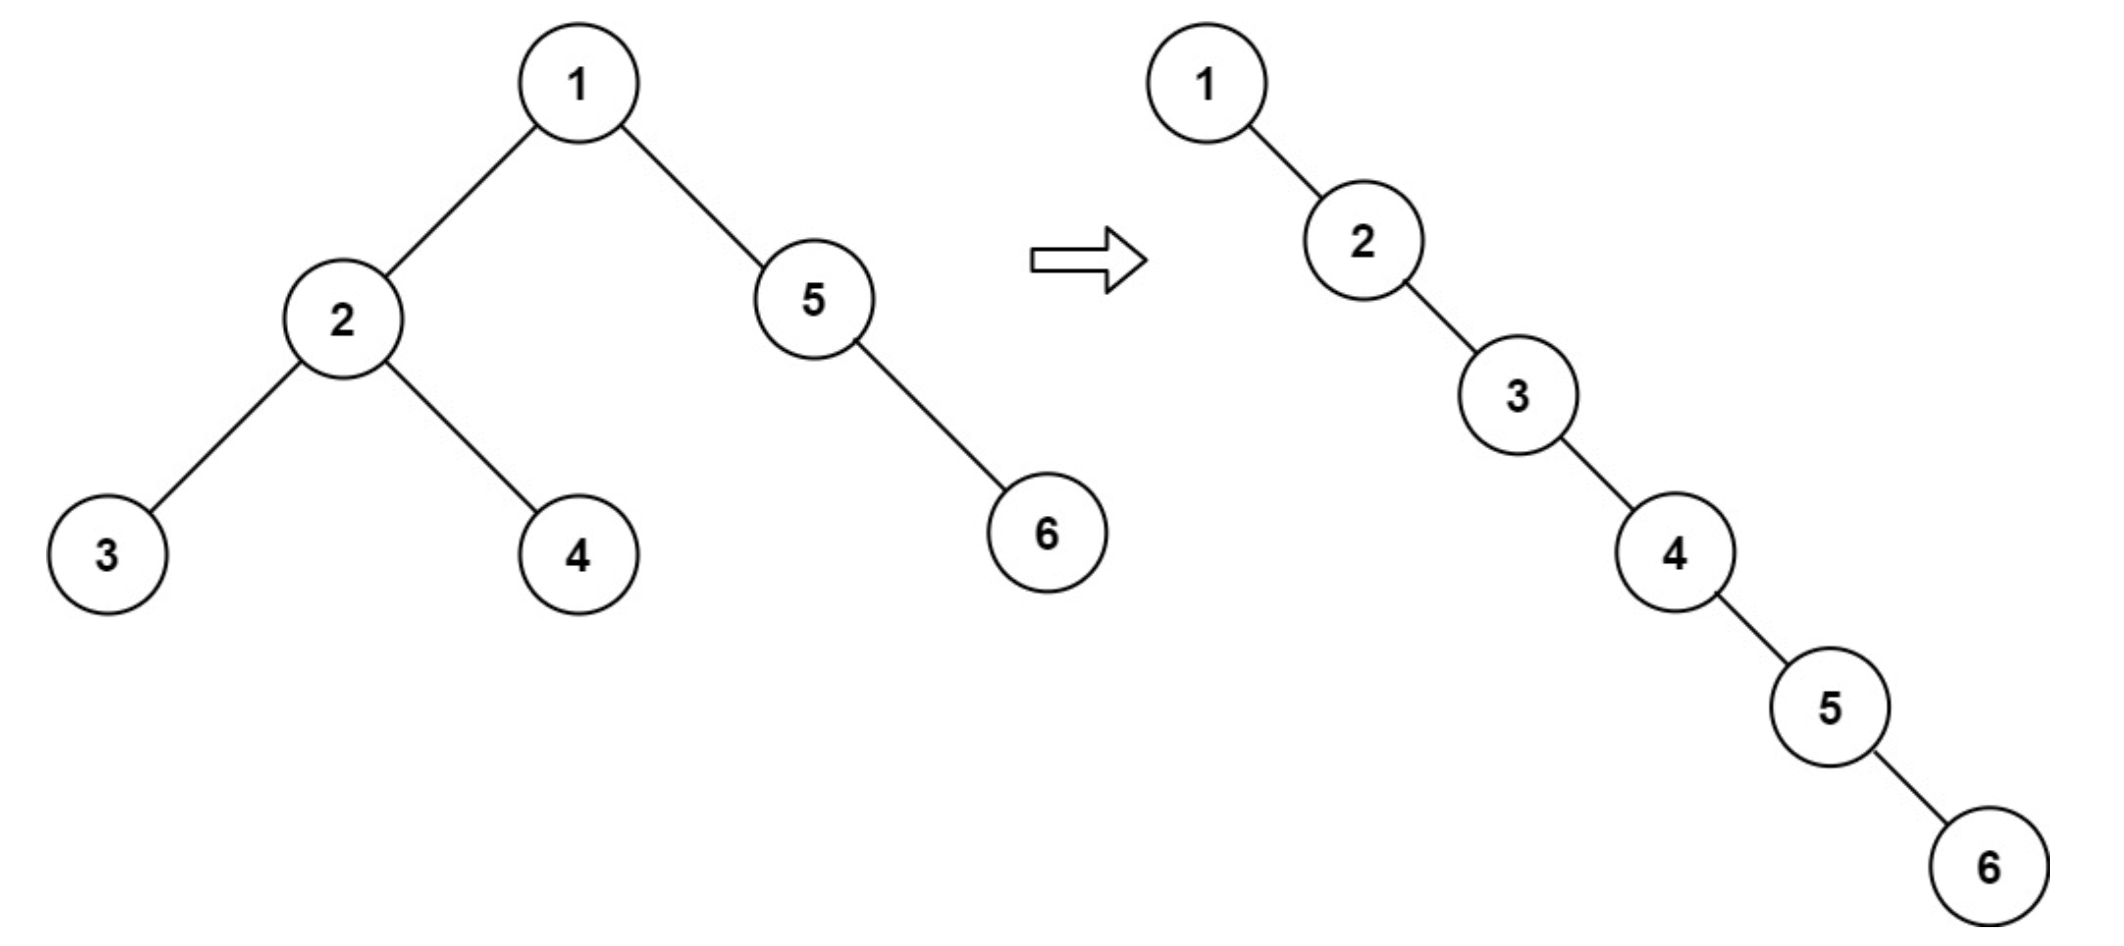
\includegraphics[width=0.8\linewidth]{images/lc0114_example}
	\label{fig:lc0114example}
\end{figure}

\subsection*{Solution - Recursion}
\begin{lstlisting}
void flatten(TreeNode* root) {
	// base case
	if (!root) { return; }
	flatten(root->left);
	flatten(root->right);
	// temporarily store the right child as it will be overwritten.
	TreeNode* temp_right = root->right;
	if (root->left) {
		// attach the left subtree to the right of the root
		root->right = root->left;
		root->left = nullptr;
		// attach the original right subtree to the tail of the new right subtree
		TreeNode* curr = root->right;
		while (curr->right) { curr = curr->right; }
		curr->right = temp_right;
	}
}
\end{lstlisting}

\section{LC 0102 - Binary Tree Level Order Traversal}
Given the {\colorbox{CodeBackground}{\lstinline|root|}} of a \ul{binary tree}, return the level order traversal of its nodes' values. (i.e., from left to right, level by level).\\

Example:
\begin{figure}[H]
	\centering
	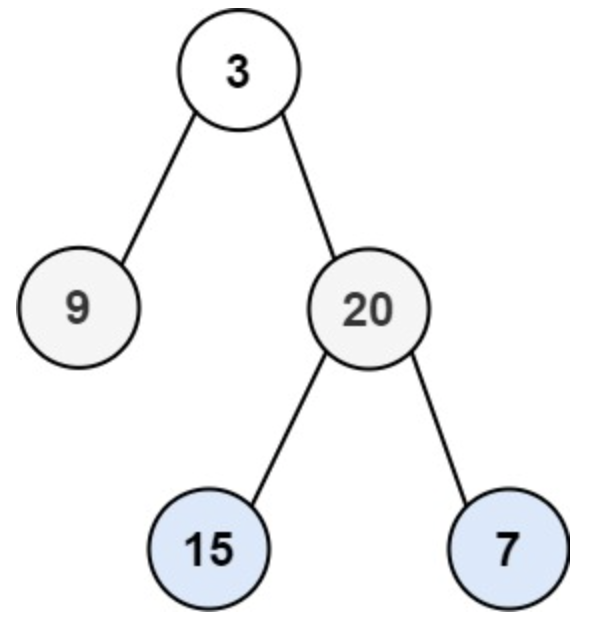
\includegraphics[width=0.25\linewidth]{images/lc0102_example}
	\label{fig:lc0102example}
\end{figure}
{\colorbox{CodeBackground}{\lstinline|--> [[3],[9,20],[15,7]]|}}

\subsection*{Solution}
\begin{lstlisting}
std::vector<std::vector<int>> levelOrder(TreeNode* root) {
	std::vector<std::vector<int>> result;
	if (!root) { return result; }
	std::queue<TreeNode*> q;
	q.push(root);
	while (!q.empty()) {
		int level_size = q.size();
		std::vector<int> curr_level;
		for (int i = 0; i < level_size; ++i) {
			TreeNode* node = q.front();
			q.pop();
			curr_level.push_back(node->val);
			if (node->left) { q.push(node->left); }
			if (node->right) { q.push(node->right); }
		}
		result.push_back(curr_level);
	}
	return result;
}
\end{lstlisting}

\section{LC 0103 - Binary Tree Zigzag Level Order Traversal}
Given the {\colorbox{CodeBackground}{\lstinline|root|}} of a \ul{binary tree}, return the \ul{zigzag level order traversal} of its nodes' values. (i.e., from left to right, then right to left for the next level and alternate between).\\

Example:
\begin{figure}[H]
	\centering
	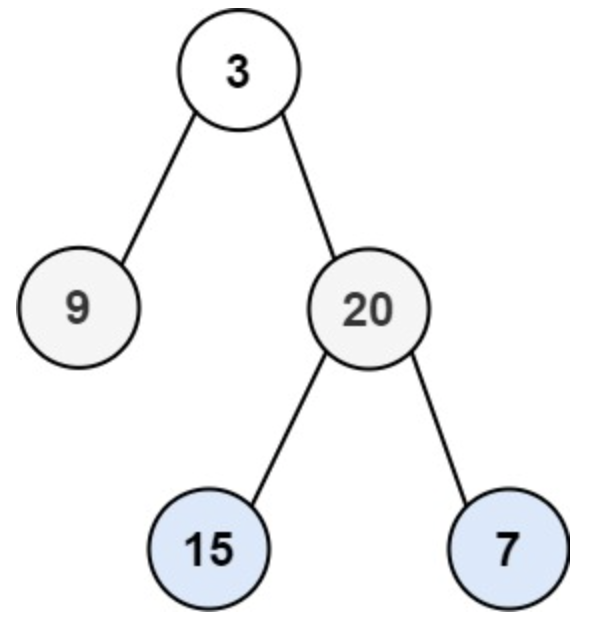
\includegraphics[width=0.25\linewidth]{images/lc0102_example}
	\label{fig:lc0102example}
\end{figure}
{\colorbox{CodeBackground}{\lstinline|--> [[3],[20,9],[15,7]]|}}

\subsection*{Solution}
\begin{lstlisting}
std::vector<std::vector<int>> zigzagLevelOrder(TreeNode* root) {
	std::vector<std::vector<int>> result;
	if (!root) { return result; }
	std::queue<TreeNode*> q;
	q.push(root);
	bool l2r = true;
	while (!q.empty()) {
		int level_size = q.size();
		std::vector<int> cur_level(level_size);
		for (int i = 0; i < level_size; ++i) {
			TreeNode* node = q.front();
			q.pop();
			int idx = (l2r) ? i : (level_size - 1 - i);
			cur_level[idx] = node->val;
			if (node->left) { q.push(node->left); }
			if (node->right) { q.push(node->right); }
		}
		l2r = !l2r;
		result.push_back(cur_level);
	}
	return result;
}
\end{lstlisting}

\section{LC 0637 - Average of Levels in Binary Tree}
Given the {\colorbox{CodeBackground}{\lstinline|root|}} of a \ul{binary tree}, return the average value of the nodes on each level in the form of an array.\\

Example:
\begin{figure}[H]
	\centering
	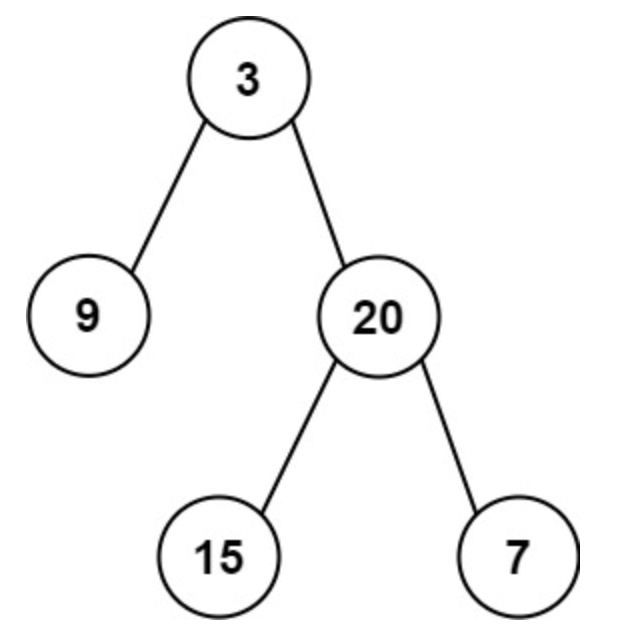
\includegraphics[width=0.25\linewidth]{images/lc0637_example}
	\label{fig:lc0637example}
\end{figure}
{\colorbox{CodeBackground}{\lstinline|--> [3.00000,14.50000,11.00000]|}}

\subsection*{Solution}
level-order traversal
\begin{lstlisting}
std::vector<double> averageOfLevels(TreeNode* root) {
	std::vector<double> avg_level;
	std::queue<TreeNode*> q;
	q.push(root);
	while (!q.empty()) {
		int level_size = q.size();
		double level_sum = 0;
		for (int i = 0; i < level_size; ++i) {
			TreeNode* curr = q.front();
			q.pop();
			level_sum += curr->val;
			if (curr->left) { q.push(curr->left); }
			if (curr->right) { q.push(curr->right); }
		}
		avg_level.push_back(level_sum / level_size);
	}
	return avg_level;
}
\end{lstlisting}

\section{LC 0199 - Binary Tree Right Side View}
Given the {\colorbox{CodeBackground}{\lstinline|root|}} of a \ul{binary tree}, imagine yourself standing on the right side of it, return the values of the nodes you can see ordered from top to bottom.\\

Example:
\begin{figure}[H]
	\centering
	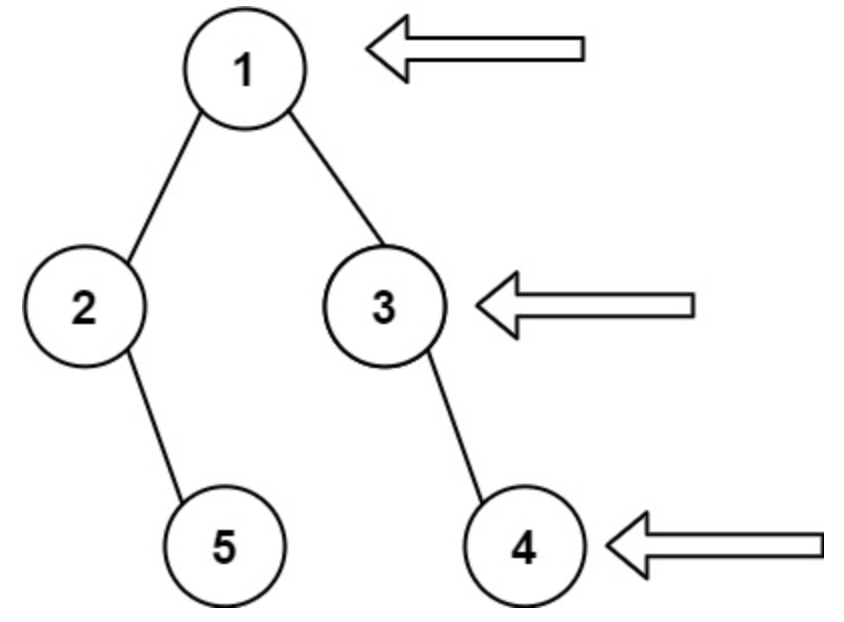
\includegraphics[width=0.33\linewidth]{images/lc0199_example}
	\label{fig:lc0199example}
\end{figure}
{\colorbox{CodeBackground}{\lstinline|--> [1,3,4]|}}

\subsection*{Solution - Iterative}
level-order traversal
\begin{lstlisting}
std::vector<int> rightSideView(TreeNode* root) {
	if (!root) { return; };
	std::vector<int> view;
	std::queue<TreeNode*> q;
	q.push(root);
	while (!q.empty()) {
		int level_size = q.size();
		for (int i = 0; i < level_size; ++i) {
			TreeNode* node = q.front();
			q.pop();
			if (i == level_size - 1) { view.push_back(node->val); }
			if (node->left) { q.push(node->left); }
			if (node->right) { q.push(node->right); }
		}
	}
	return view;
}
\end{lstlisting}

\subsection*{Solution - Recursion}
\begin{lstlisting}
std::vector<int> rightSideView(TreeNode* root) {
	std::vector<int> view;
	rightViewDFS(root, 0, view);
	return view;
}

void rightViewDFS(TreeNode* node, int level, std::vector<int>& view) {
	if (!node) { return; }
	// first time we've reached this level
	if (level == view.size()) { view.push_back(node->val); }
	// prioritize right subtree, then left subtree.
	rightViewDFS(node->right, level + 1, view);
	rightViewDFS(node->left, level + 1, view);
}
\end{lstlisting}

\section{LC 0117 - Populating Next Right Pointers in Each Node II}
Given a \ul{binary tree}:
\begin{lstlisting}
struct Node {
	int val;
	Node *left;
	Node *right;
	Node *next;
};
\end{lstlisting}
Populate each next pointer to point to its next right node. If there is no next right node, the next pointer should be set to {\colorbox{CodeBackground}{\lstinline|nullptr|}}. Initially, all next pointers are set to {\colorbox{CodeBackground}{\lstinline|nullptr|}}.\\

Example:
\begin{figure}[H]
	\centering
	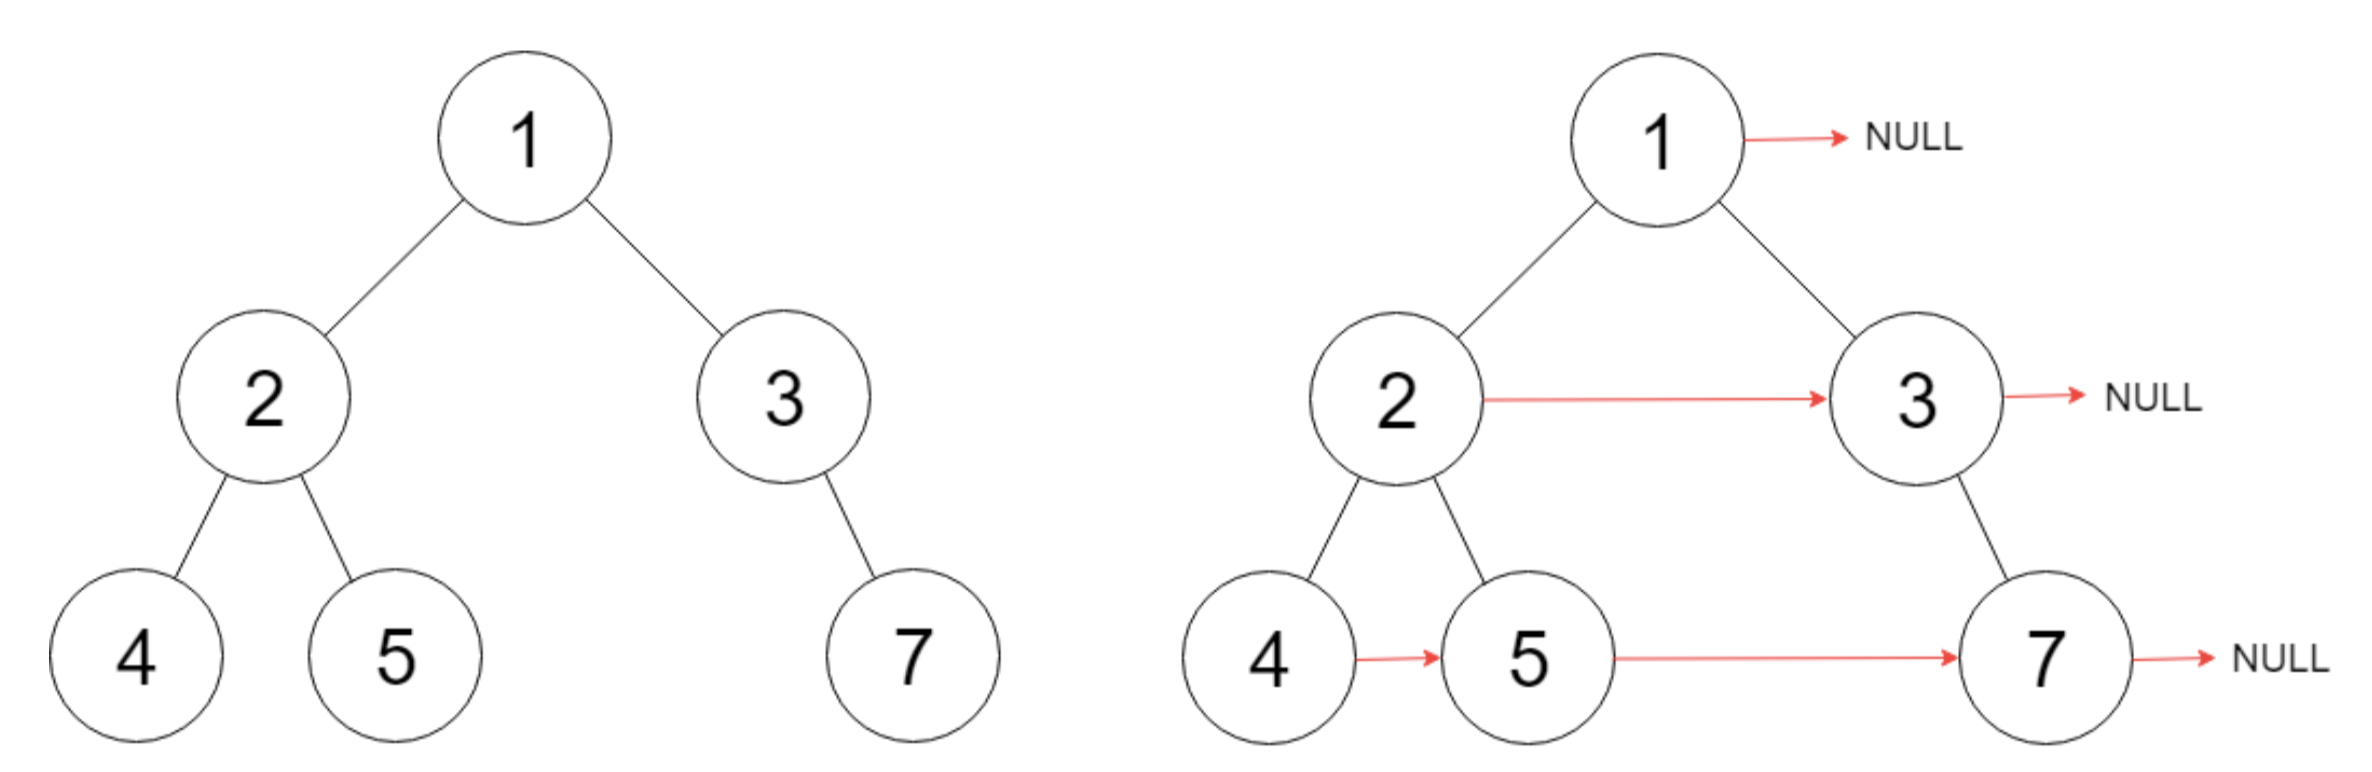
\includegraphics[width=0.65\linewidth]{images/lc0117_example}
	\label{fig:lc0117example}
\end{figure}

\subsection*{Solution}
level-order traversal
\begin{lstlisting}
Node* connect(Node* root) {
	if (!root) { return root; }
	std::queue<Node*> q;
	q.push(root);
	while (!q.empty()) {
		Node* prev = nullptr;
		int level_size = q.size();
		for (int i = 0; i < level_size; ++i) {
			Node* curr = q.front();
			q.pop();
			if (prev) { prev->next = curr; }
			prev = curr;
			if (curr->left) { q.push(curr->left); }
			if (curr->right) { q.push(curr->right); }
		}
		prev->next = nullptr;
	}
	return root;
}
\end{lstlisting}

\section{LC 0112 - Path Sum}\label{lc0112}
Given the {\colorbox{CodeBackground}{\lstinline|root|}} of a \ul{binary tree} and an integer {\colorbox{CodeBackground}{\lstinline|targetSum|}}, return {\colorbox{CodeBackground}{\lstinline|true|}} if the tree has a \ul{root-to-leaf path} such that adding up all the values along the path equals {\colorbox{CodeBackground}{\lstinline|targetSum|}}.\\

Example:
\begin{figure}[H]
	\centering
	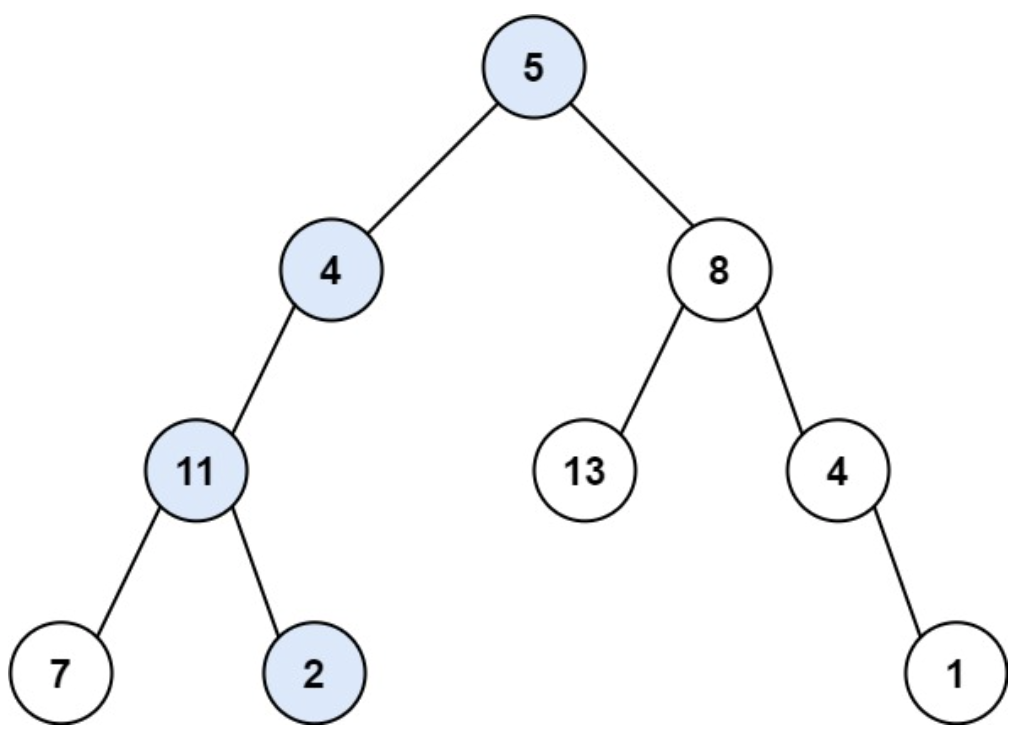
\includegraphics[width=0.5\linewidth]{images/lc0112}
	\label{fig:lc0112}
\end{figure}
{\colorbox{CodeBackground}{\lstinline|root = [5,4,8,11,null,13,4,7,2,null,null,null,1], targetSum = 22 --> true|}}

\subsection*{Solution - Recursion}
\begin{lstlisting}
bool hasPathSum(TreeNode* root, int targetSum) {
	// base case 1: child of leaf node
	if (!root) { return false; }
	// base case 2: leaf node
	if (!root->left && !root->right) { return root->val == targetSum; }
	return hasPathSum(root->left, targetSum - root->val)
	|| hasPathSum(root->right, targetSum - root->val);
}
\end{lstlisting}

\subsection*{Related}
\begin{itemize}
	\item \hyperref[lc0120]{[Binary Tree] LC 0120 - Triangle}
	\item \hyperref[lc0112]{[Binary Tree] LC 0112 - Path Sum}
	\item \hyperref[lc0124]{[Binary Tree] LC 0124 - Binary Tree Maximum Path Sum}
	\item \hyperref[lc0064]{[Matrix] LC 0064 - Minimum Path Sum}
\end{itemize}

\section{LC 0129 - Sum Root to Leaf Numbers}
You are given the {\colorbox{CodeBackground}{\lstinline|root|}} of a \ul{binary tree} containing digits from {\colorbox{CodeBackground}{\lstinline|0|}} to {\colorbox{CodeBackground}{\lstinline|9|}} only.\\

Each \ul{root-to-leaf path} in the tree represents a number.\\

For example, the \ul{root-to-leaf path} {\colorbox{CodeBackground}{\lstinline|1 --> 2 --> 3|}} represents the number {\colorbox{CodeBackground}{\lstinline|123|}}.\\

Return the total sum of all \ul{root-to-leaf numbers}.\\

Example:
\begin{figure}[H]
	\centering
	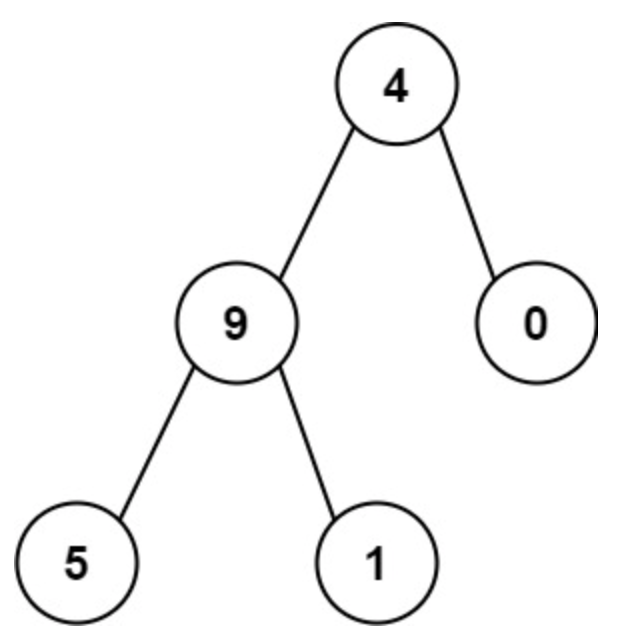
\includegraphics[width=0.23\linewidth]{images/lc0129_example}
	\label{fig:lc0129example}
\end{figure}
{\colorbox{CodeBackground}{\lstinline|root = [4,9,0,5,1] --> 1026 (495 + 491 + 40)|}}

\subsection*{Solution}
\begin{lstlisting}
int sumNumbers(TreeNode* root) { return sumNumbersRecursive(root, 0); }

int sumNumbersRecursive(TreeNode* node, int cur_sum) {
	// base case 1: child of leaf node
	if (!node) { return 0; }
	cur_sum = cur_sum * 10 + node->val;
	// base case 2: leaf node
	if (!node->left && !node->right) { return cur_sum; }
	return sumNumbersRecursive(node->left, cur_sum) 
	+ sumNumbersRecursive(node->right, cur_sum);
}
\end{lstlisting}

\section{LC 0124 - Binary Tree Maximum Path Sum}\label{lc0124}
A \ul{path} in a \ul{binary tree} is a sequence of nodes where each pair of \ul{adjacent nodes} in the sequence has an \ul{edge} connecting them. A node can only appear in the sequence at most once. Note that the path does not need to pass through the root.\\

The \ul{path sum} of a path is the sum of the node's values in the path.\\

Given the {\colorbox{CodeBackground}{\lstinline|root|}} of a binary tree, return the \ul{maximum path sum} of any non-empty path.\\

Example:
\begin{figure}[H]
	\centering
	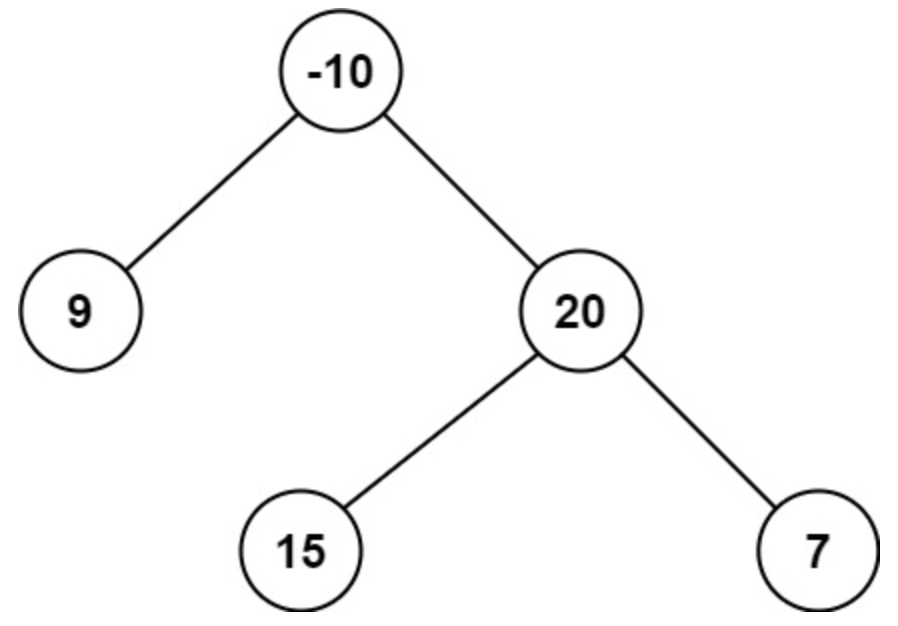
\includegraphics[width=0.35\linewidth]{images/lc0124_example}
	\label{fig:lc0124example}
\end{figure}
{\colorbox{CodeBackground}{\lstinline|root = [-10,9,20,null,null,15,7] --> 42 (15 + 20 + 7)|}}

\subsection*{Solution}
The recursive function {\colorbox{CodeBackground}{\lstinline|maxPathDown|}} does more than just calculate the maximum path sum starting from the root. More importantly, it explores all potential paths throughout the tree, evaluating each for the maximum path sum we're seeking.
\begin{lstlisting}
int maxPathSum(TreeNode* root) {
	int max_sum = std::numeric_limits<int>::min();
	maxPathDown(root, max_sum);
	return max_sum;
}

// calculate maximum path sum starting from root and update max_sum
int maxPathDown(TreeNode* root, int& max_sum) {
	// base case: child of leaf node
	if (!root) { return 0; }
	// maximum path sum starting from left and right child, set to zero if negative
	int left = std::max(0, maxPathDown(root->left, max_sum));
	int right = std::max(0, maxPathDown(root->right, max_sum));
	// update max_sum
	max_sum = std::max(max_sum, root->val + left + right);
	// return maximum path sum starting from root
	return std::max(left, right) + root->val;
}
\end{lstlisting}

\subsection*{Related}
\begin{itemize}
	\item \hyperref[lc0120]{[Binary Tree] LC 0120 - Triangle}
	\item \hyperref[lc0112]{[Binary Tree] LC 0112 - Path Sum}
	\item \hyperref[lc0124]{[Binary Tree] LC 0124 - Binary Tree Maximum Path Sum}
	\item \hyperref[lc0064]{[Matrix] LC 0064 - Minimum Path Sum}
\end{itemize}

\section{LC 0958 - Check Completeness of a Binary Tree}\label{lc0958}
Given the root of a binary tree, determine if it is a \ul{complete binary tree}.

\subsection*{Solution}
level-order traversal $+$ state {\colorbox{CodeBackground}{\lstinline|bool null_seen|}}
\begin{lstlisting}
int countNodes(TreeNode* root) {
	if (!root) { return 0; }
	int left_h = 0;
	int right_h = 0;
	TreeNode* left = root;
	TreeNode* right = root;
	while (left) {
		++left_h;
		left = left->left;
	}
	while (right) {
		++right_h;
		right = right->right;
	}
	// full binary tree
	if (left_h == right_h) { return (1 << left_h) - 1; }
	// non-full complete binary tree
	return 1 + countNodes(root->left) + countNodes(root->right);
}
\end{lstlisting}

\subsection*{Related}
\begin{itemize}
	\item \hyperref[lc0958]{LC 0958 - Check Completeness of a Binary Tree}
	\item \hyperref[lc0098]{LC 0098 - Validate BST}
\end{itemize}

\section{LC 0222 - Count Complete Tree Nodes}
Given the {\colorbox{CodeBackground}{\lstinline|root|}} of a \ul{complete binary tree}, return the number of the nodes in the tree.\\

Design an algorithm that runs in less than {\colorbox{CodeBackground}{\lstinline|O(n)|}} time complexity where {\colorbox{CodeBackground}{\lstinline|n|}} is the number of nodes of the tree.\\

Example:
\begin{figure}[H]
	\centering
	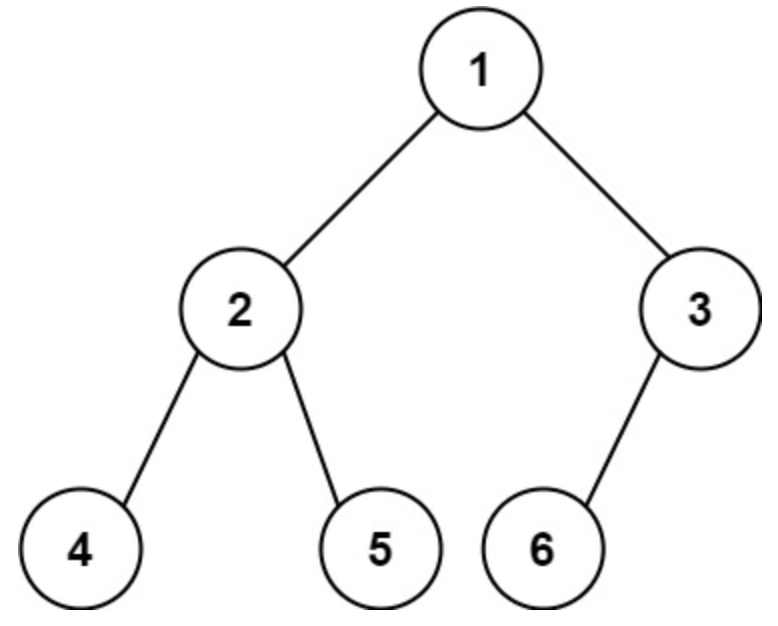
\includegraphics[width=0.32\linewidth]{images/lc0222_example}
	\label{fig:lc0222example}
\end{figure}
{\colorbox{CodeBackground}{\lstinline|--> 6|}}

\subsection*{Solution - Recursion}
\begin{lstlisting}
int countNodes(TreeNode* root) {
	if (!root) { return 0; }
	int left_h = 0;
	int right_h = 0;
	TreeNode* left = root;
	TreeNode* right = root;
	while (left) {
		++left_h;
		left = left->left;
	}
	while (right) {
		++right_h;
		right = right->right;
	}
	// base case: full binary tree
	if (left_h == right_h) { return (1 << left_h) - 1; }
	// non-full complete binary tree
	return 1 + countNodes(root->left) + countNodes(root->right);
}
\end{lstlisting}

\section{LC 0098 - Validate BST}\label{lc0098}
Given the {\colorbox{CodeBackground}{\lstinline|root|}} of a \ul{binary tree}, determine if it is a valid \ul{binary search tree (BST)}.\\

A valid BST is defined as follows:
\begin{itemize}
	\item The left subtree of a node contains only nodes with keys less than the node's key.
	\item The right subtree of a node contains only nodes with keys greater than the node's key.
	\item Both the left and right subtrees must also be binary search trees.
\end{itemize}

\subsection*{Solution 1 - In-order Traversal (Recursive)}
\begin{lstlisting}
bool isValidBST(TreeNode* root) {
	long prev_val = LONG_MIN;
	return InorderCheck(root, prev_val);
}

bool InorderCheck(TreeNode* node, long& prev_val) {
	if (!node) { return true; }
	if (!InorderCheck(node->left, prev_val)) { return false; }
	if (node->val <= prev_val) { return false; }
	prev_val = node->val;
	return InorderCheck(node->right, prev_val);
}
\end{lstlisting}

\subsection*{Solution 2 - In-order Traversal (Iterative)}
\begin{lstlisting}
bool isValidBST(TreeNode* root) {
	if (!root) { return true; }
	std::stack<TreeNode*> stk;
	long prev_val = LONG_MIN;
	TreeNode* curr = root;
	while (curr || !stk.empty()) {
		while (curr) {
			stk.push(curr);
			curr = curr->left;
		}
		TreeNode* top = stk.top();
		stk.pop();
		if (top->val <= prev_val) { return false; }
		prev_val = top->val;
		curr = top->right;
	}
	return true;
}
\end{lstlisting}

\subsection*{Solution 3 - Value Range Check}
\begin{lstlisting}
bool isValidBST(TreeNode* root) { return validateBST(root, LONG_MIN, LONG_MAX); }

bool validateBST(TreeNode* node, long min_val, long max_val) {
	if (!node) { return true; }
	if (node->val <= min_val || node->val >= max_val) { return false; }
	return validateBST(node->left, min_val, node->val)
				 && validateBST(node->right, node->val, max_val);
}
\end{lstlisting}

\subsection*{Related}
\begin{itemize}
	\item \hyperref[lc0958]{LC 0958 - Check Completeness of a Binary Tree}
	\item \hyperref[lc0098]{LC 0098 - Validate BST}
\end{itemize}

\section{LC 0230 - Kth Smallest Element in a BST}
Given the {\colorbox{CodeBackground}{\lstinline|root|}} of a \ul{binary search tree (BST)}, and an integer {\colorbox{CodeBackground}{\lstinline|k|}}, return the {\colorbox{CodeBackground}{\lstinline|k|}}th smallest value ({\colorbox{CodeBackground}{\lstinline|1|}}-indexed) of all the values of the nodes in the tree.

\subsection*{Solution 1 - In-order Traversal (Recursive)}
\begin{lstlisting}
int kthSmallest(TreeNode* root, int k) {
	int count = 0;
	int result = -1;
	InorderTraverse(root, k, count, result);
	return result;
}

void InorderTraverse(TreeNode* node, int k, int& count, int& result) {
	if (!node || count >= k) { return; }
	InorderTraverse(node->left, k, count, result);
	if (++count == k) {
		result = node->val;
		return;
	}
	InorderTraverse(node->right, k, count, result);
}
\end{lstlisting}

\subsection*{Solution 2 - In-order Traversal (Iterative)}
\begin{lstlisting}
int kthSmallest(TreeNode* root, int k) {
	if (!root) { return -1; }
	std::stack<TreeNode*> stk;
	TreeNode* curr = root;
	int count = 0;
	while (curr || !stk.empty()) {
		while (curr) {
			stk.push(curr);
			curr = curr->left;
		}
		TreeNode* top = stk.top();
		stk.pop();
		if (++count == k) { return top->val; }
		curr = top->right;
	}
	return -1;
}
\end{lstlisting}

\section{LC 0530 - Minimum Absolute Difference in BST}
Given the {\colorbox{CodeBackground}{\lstinline|root|}} of a \ul{Binary Search Tree (BST)}, return the minimum absolute difference between the values of any two different nodes in the tree.\\

Example:
\begin{figure}[H]
	\centering
	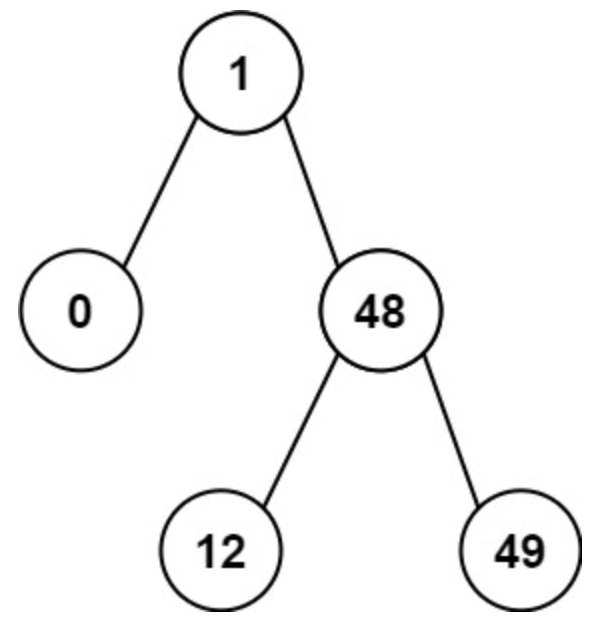
\includegraphics[width=0.25\linewidth]{images/lc0530_example}
	\label{fig:lc0530example}
\end{figure}
{\colorbox{CodeBackground}{\lstinline|--> 1|}}

\subsection*{Solution 1 - In-order Traversal (Recursive)}
\begin{lstlisting}
int getMinimumDifference(TreeNode* root) {
	int min_diff = std::numeric_limits<int>::max();
	TreeNode* prev = nullptr;
	InorderTraverse(root, prev, min_diff);
	return min_diff;
}

void InorderTraverse(TreeNode* node, TreeNode*& prev, int& min_diff) {
	if (!node) { return; }
	InorderTraverse(node->left, prev, min_diff);
	if (prev) { min_diff = std::min(min_diff, node->val - prev->val); }
	prev = node;
	InorderTraverse(node->right, prev, min_diff);
}
\end{lstlisting}

\subsection*{Solution 2 - In-order Traversal (Iterative)}
\begin{lstlisting}
int getMinimumDifference(TreeNode* root) {
	if (!root) { return -1; }
	std::stack<TreeNode*> stk;
	TreeNode* curr = root;
	TreeNode* prev = nullptr;
	int min_diff = std::numeric_limits<int>::max();
	while (curr || !stk.empty()) {
		while (curr) {
			stk.push(curr);
			curr = curr->left;
		}
		TreeNode* top = stk.top();
		stk.pop();
		if (prev) { min_diff = std::min(min_diff, top->val - prev->val); }
		prev = top;
		curr = top->right;
	}
	return min_diff;
}
\end{lstlisting}

\section{LC 0173 - BST Iterator}
Implement the {\colorbox{CodeBackground}{\lstinline|BSTIterator|}} class that represents an iterator over the \ul{in-order traversal} of a \ul{binary search tree (BST)}:
\begin{itemize}
	\item {\colorbox{CodeBackground}{\lstinline|BSTIterator(TreeNode root)|}} - Initializes an object of the {\colorbox{CodeBackground}{\lstinline|BSTIterator|}} class. The {\colorbox{CodeBackground}{\lstinline|root|}} of the BST is given as part of the constructor. The pointer should be initialized to a non-existent number smaller than any element in the BST.
	\item {\colorbox{CodeBackground}{\lstinline|int next()|}} - Moves the pointer to the right, then returns the number at the pointer. Notice that the first call to {\colorbox{CodeBackground}{\lstinline|next()|}} will return the smallest element in the BST.
	\item {\colorbox{CodeBackground}{\lstinline|boolean hasNext()|}} - Returns {\colorbox{CodeBackground}{\lstinline|true|}} if there exists a number in the traversal to the right of the pointer, otherwise returns {\colorbox{CodeBackground}{\lstinline|false|}}.
\end{itemize}


\begin{lstlisting}
class BSTIterator {
 public:
	BSTIterator(TreeNode* root) { PushAll(root); }
	
	/** @return the next smallest number */
	int next() {
		TreeNode* top = stk.top();
		stk.pop();
		PushAll(top->right);
		return top->val;
	}
	
	/** @return whether we have a next smallest number */
	bool hasNext() { return !stk.empty(); }
	
 private:
	void PushAll(TreeNode* node) {
		while (node) {
			stk.push(node);
			node = node->left;
		}
	}
	
	std::stk<TreeNode*> stk;
};
\end{lstlisting}

\section{LC 0235 - Lowest Common Ancestor of a BST}\label{lc0235}
Given a \ul{binary search tree (BST)}, find the \ul{lowest common ancestor (LCA)} node of two given nodes in the BST. Note that both {\colorbox{CodeBackground}{\lstinline|p|}} and {\colorbox{CodeBackground}{\lstinline|q|}} are in the tree and {\colorbox{CodeBackground}{\lstinline|p != q|}}.\\

Definition of LCA: The \ul{lowest common ancestor (LCA)} is defined between two nodes {\colorbox{CodeBackground}{\lstinline|p|}} and {\colorbox{CodeBackground}{\lstinline|q|}} as the lowest node in the tree that has both {\colorbox{CodeBackground}{\lstinline|p|}} and {\colorbox{CodeBackground}{\lstinline|q|}} as \ul{descendants} (where we allow a node to be a \ul{descendant} of itself). \\

Example:

\begin{figure}[H]
	\centering
	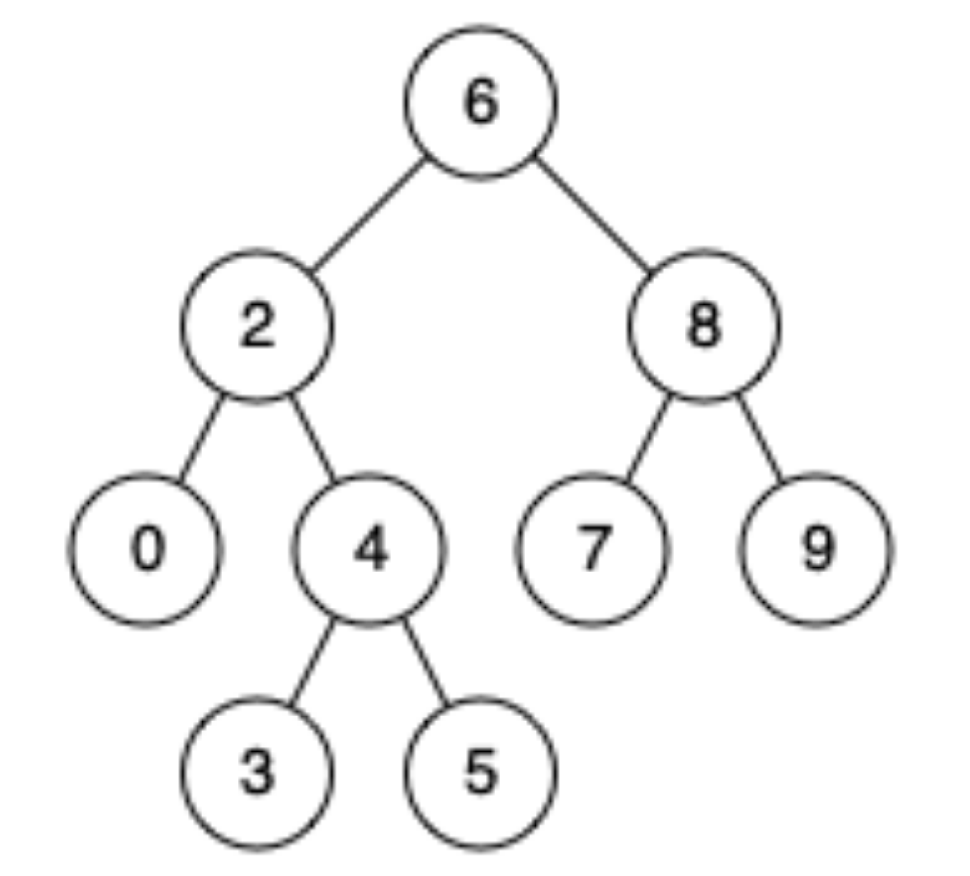
\includegraphics[width=0.3\linewidth]{images/lc0235_example}
	\label{fig:lc0235example}
\end{figure}
\begin{lstlisting}
	p = 2, q = 8 --> 6
	p = 2, q = 4 --> 2
\end{lstlisting}

\subsection*{Solution}
\begin{lstlisting}
TreeNode* lowestCommonAncestor(TreeNode* root, TreeNode* p, TreeNode* q) {
	TreeNode* curr = root;
	while (curr) {
		if (p->val > curr->val && q->val > curr->val) {
			curr = curr->right;
		} else if (p->val < curr->val && q->val < curr->val) {
			curr = curr->left;
		} else {
			return curr;
		}
	}
	return nullptr;
}
\end{lstlisting}

\subsection*{Related}
\begin{itemize}
	\item \hyperref[lc0236]{LC 0236 - Lowest Common Ancestor of a Binary Tree}
	\item \hyperref[lc0235]{LC 0235 - Lowest Common Ancestor of a BST}
\end{itemize}

\section{LC 0110 - Balanced Binary Tree}
Given a \ul{binary tree}, determine if it is \ul{height-balanced}.

\section{LC 0257 - Binary Tree Paths}
Given the {\colorbox{CodeBackground}{\lstinline|root|}} of a \ul{binary tree}, return all \ul{root-to-leaf paths} in any order.\\

\begin{itemize}
\item Example 1: {\colorbox{CodeBackground}{\lstinline|root = [1,2,3,null,5] --> ["125","13"]|}}
\begin{figure}[H]
\centering
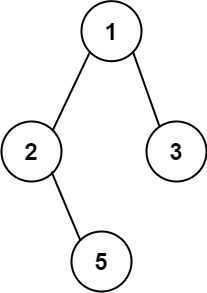
\includegraphics[width=0.16\linewidth]{images/lc0257_eg}
\label{fig:lc0257eg}
\end{figure}
\item Example 2: {\colorbox{CodeBackground}{\lstinline|root = [1] --> ["1"]|}}
\end{itemize}

\section{LC 0404 - Sum of Left Leaves}
Given the {\colorbox{CodeBackground}{\lstinline|root|}} of a \ul{binary tree}, return the sum of all left leaves.\\

\begin{itemize}
\item Example 1: {\colorbox{CodeBackground}{\lstinline|root = [3,9,20,null,null,15,7] --> 24 (9 + 15)|}}
\begin{figure}[H]
\centering
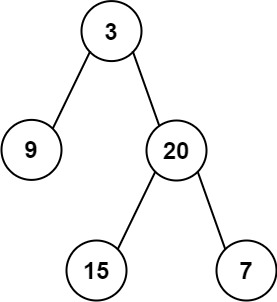
\includegraphics[width=0.22\linewidth]{images/lc0404_eg}
\label{fig:lc0404eg}
\end{figure}
\item Example 2: {\colorbox{CodeBackground}{\lstinline|root = [1] --> 0|}}
\end{itemize}

\section{LC 0513 - Find Bottom Left Tree Value}
Given the {\colorbox{CodeBackground}{\lstinline|root|}} of a\ul{ binary tree}, return the leftmost value \ul{in the last row of the tree}.

\begin{itemize}
\item Example 1: {\colorbox{CodeBackground}{\lstinline|root = [2,1,3] --> 1|}}
\begin{figure}[H]
\centering
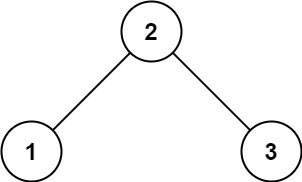
\includegraphics[width=0.25\linewidth]{images/lc0513_eg1}
\label{fig:lc0513eg1}
\end{figure}
\item Example 2: {\colorbox{CodeBackground}{\lstinline|root = [1,2,3,4,null,5,6,null,null,7] --> 7|}}
\begin{figure}[H]
\centering
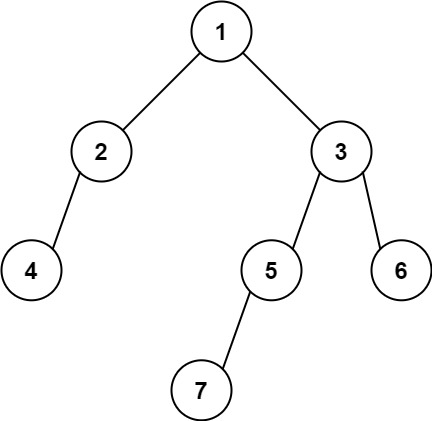
\includegraphics[width=0.35\linewidth]{images/lc0513_eg2}
\label{fig:lc0513eg2}
\end{figure}
\end{itemize}

\section{LC 0654 - Maximum Binary Tree}
You are given an integer array {\colorbox{CodeBackground}{\lstinline|nums|}} with no duplicates. A maximum binary tree can be built recursively from {\colorbox{CodeBackground}{\lstinline|nums|}} using the following algorithm:
\begin{itemize}
\item Create a root node whose value is the maximum value in {\colorbox{CodeBackground}{\lstinline|nums|}}.
\item Recursively build the left subtree on the subarray prefix to the left of the maximum value.
\item Recursively build the right subtree on the subarray suffix to the right of the maximum value.
\end{itemize}
Return the maximum binary tree built from {\colorbox{CodeBackground}{\lstinline|nums|}}.\\

\begin{itemize}
\item Example 1: {\colorbox{CodeBackground}{\lstinline|nums = [3,2,1,6,0,5]|}}
\begin{figure}[H]
\centering
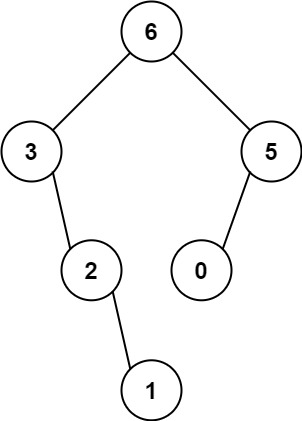
\includegraphics[width=0.25\linewidth]{images/lc0654_eg1}
\label{fig:lc0654eg1}
\end{figure}
\item Example 2: {\colorbox{CodeBackground}{\lstinline|nums = [3,2,1]|}}
\begin{figure}[H]
\centering
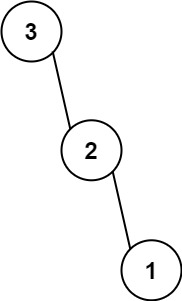
\includegraphics[width=0.15\linewidth]{images/lc0654_eg2}
\label{fig:lc0654eg2}
\end{figure}
\end{itemize}

\section{LC 0617 - Merge Two Binary Trees}

\section{LC 0700 - Search in a Binary Search Tree}

\section{LC 0501 - Find Mode in Binary Search Tree}

\section{LC 0701 - Insert into a Binary Search Tree}

\section{LC 0450 - Delete Node in a BST}

\section{LC 0669 - Trim a Binary Search Tree}

\section{LC 0108 - Convert Sorted Array to Binary Search Tree}

\section{LC 0538 - Convert BST to Greater Tree}

\section{LC 0107 - Binary Tree Level Order Traversal II}

\section{LC 0429 - N-ary Tree Level Order Traversal}

\section{LC 0515 - Find Largest Value in Each Tree Row}

\section{LC 0116 - Populating Next Right Pointers in Each Node}
\chapter{Graph}
\section{Thinking in Graphs}
Since graphs are very common in daily life, we should be able to translate real-world problems into graph-related terms.

\subsubsection*{Takeaway}
When designing a BFS algorithm, you should:
\begin{itemize}
\item Carefully check the neighboring nodes, only enqueue those that are valid for exploration.
\item For any conditions or states influencing the decision to explore a neighboring node, update these states as soon as possible.
\end{itemize}

\section{LC 0133 - Clone Graph}\label{lc0133}
Given a pointer of a node in a {\color{blue}{connected undirected graph}}, return a {\color{blue}{deep copy}} of the graph. \\

The definition of {\colorbox{CodeBackground}{\lstinline|Node|}} is as follows.
\begin{lstlisting}
class Node {
 public:
	Node() {
		val = 0;
		neighbors = std::vector<Node*>();
	}
	Node(int _val) {
		val = _val;
		neighbors = std::vector<Node*>();
	}
	Node(int _val, std::vector<Node*> _neighbors) {
		val = _val;
		neighbors = _neighbors;
	}
	
	int val;
	std::vector<Node*> neighbors;
};
\end{lstlisting}

\subsection*{Analysis}
We cannot borrow algorithms from
\hyperref[chap:graph_boilerplate]{Chapter \ref{chap:graph_boilerplate}} directly because deep copy of a node can only be done after all its neighbors are traversed. This means the visit of current node are mixed up with further visit of its neighbors.

\subsection*{Solution 1 - BFS}
\begin{lstlisting}
	Node* cloneGraph(Node* node) {
		if (!node) { return nullptr; }
		std::queue<Node*> q;
		std::unordered_map<Node*, Node*> origin2copy;
		q.push(node);
		// shallow copy
		origin2copy[node] = new Node(node->val);
		while (!q.empty()) {
			Node* front = q.front();
			q.pop();
			for (auto& neighbor : front->neighbors) {
				if (origin2copy.find(neighbor) == origin2copy.end()) {
					origin2copy[neighbor] = new Node(neighbor->val);
					q.push(neighbor);
				}
				// deep copy can only be done after all its neighbors are traversed
				origin2copy[front]->neighbors.push_back(origin2copy[neighbor]);
			}
		}
		return origin2copy[node];
	}
\end{lstlisting}

\subsection*{Solution 2 - DFS}
\begin{lstlisting}
Node* cloneGraph(Node* node) {
	std::unordered_map<Node*, Node*> origin2copy;
	return cloneGraph(node, origin2copy);
}

Node* cloneGraph(Node* node, std::unordered_map<Node*, Node*>& origin2copy) {
	if (!node) { return nullptr; }
	if (origin2copy.find(node) == origin2copy.end()) {
		// shallow copy
		origin2copy[node] = new Node(node->val);
		for (auto& neighbor : node->neighbors) {
			// deep copy can only be done after all its neighbors are traversed
			origin2copy[node]->neighbors.push_back(cloneGraph(neighbor, origin2copy));
		}
	}
	return origin2copy[node];
}
\end{lstlisting}

\subsection*{Solution 3 - DFS with {\colorbox{CodeBackground}{\lstinline|static|}} Variable}
\begin{lstlisting}
Node* cloneGraph(Node* node) {
	if (!node) { return nullptr; }
	static std::unordered_map<Node*, Node*> origin2copy;
	if (origin2copy.find(node) == origin2copy.end()) {
		// shallow copy
		origin2copy[node] = new Node(node->val);
		for (auto& neighbor : node->neighbors) {
			// deep copy can only be done after all its neighbors are traversed
			origin2copy[node]->neighbors.push_back(cloneGraph(neighbor));
		}
	}
	return origin2copy[node];
}
\end{lstlisting}

\subsection*{Related}
\begin{itemize}
	\item \hyperref[lc0138]{LC 0138 - Copy List with Random Pointer}
	\item \hyperref[lc0133]{LC 0133 - Clone Graph}
\end{itemize}

\section{LC 0127 - Word Ladder}
A transformation sequence from word {\colorbox{CodeBackground}{\lstinline|beginWord|}} to word {\colorbox{CodeBackground}{\lstinline|endWord|}} ({\colorbox{CodeBackground}{\lstinline|beginWord != endWord|}}) using a dictionary {\colorbox{CodeBackground}{\lstinline|wordList|}} is a sequence of words {\colorbox{CodeBackground}{\lstinline|beginWord|}}$\rightarrow${\colorbox{CodeBackground}{\lstinline|s1|}}$\rightarrow${\colorbox{CodeBackground}{\lstinline|s2|}}$\rightarrow${\colorbox{CodeBackground}{\lstinline|s3|}}$\dots\rightarrow\dots${\colorbox{CodeBackground}{\lstinline|sk|}} such that:
\begin{itemize}
	\item Every adjacent pair of words differs by a single letter.
	\item Every {\colorbox{CodeBackground}{\lstinline|s_i|}} for {\colorbox{CodeBackground}{\lstinline|1 <= i <= k|}} is in {\colorbox{CodeBackground}{\lstinline|wordList|}}. Note that {\colorbox{CodeBackground}{\lstinline|beginWord|}} does not need to be in {\colorbox{CodeBackground}{\lstinline|wordList|}}.
	\item {\colorbox{CodeBackground}{\lstinline|s_k == endWord|}}
\end{itemize}
Given two words, {\colorbox{CodeBackground}{\lstinline|beginWord|}} and {\colorbox{CodeBackground}{\lstinline|endWord|}}, and a dictionary {\colorbox{CodeBackground}{\lstinline|wordList|}}, return the number of words in the shortest transformation sequence from {\colorbox{CodeBackground}{\lstinline|beginWord|}} to {\colorbox{CodeBackground}{\lstinline|endWord|}}, or {\colorbox{CodeBackground}{\lstinline|0|}} if no such sequence exists.\\

Examples:
\begin{itemize}
	\item {\colorbox{CodeBackground}{\lstinline|beginWord = "hit", endWord = "cog", wordList = ["hot","dot","dog","lot","log","cog"] --> 5|}}
	\item {\colorbox{CodeBackground}{\lstinline|beginWord = "hit", endWord = "cog", wordList = ["hot","dot","dog","lot","log"] --> 0|}}
\end{itemize}

\subsection*{Translate into Graph Problem}

\subsection*{Solution}

\section{LC 0126 - Word Ladder II}
A transformation sequence from word {\colorbox{CodeBackground}{\lstinline|beginWord|}} to word {\colorbox{CodeBackground}{\lstinline|endWord|}} using a dictionary {\colorbox{CodeBackground}{\lstinline|wordList|}} is a sequence of words {\colorbox{CodeBackground}{\lstinline|beginWord|}}$\rightarrow${\colorbox{CodeBackground}{\lstinline|s1|}}$\rightarrow${\colorbox{CodeBackground}{\lstinline|s2|}}$\rightarrow${\colorbox{CodeBackground}{\lstinline|s3|}}$\dots\rightarrow\dots${\colorbox{CodeBackground}{\lstinline|sk|}} such that:
\begin{itemize}
	\item Every adjacent pair of words differs by a single letter.
	\item Every {\colorbox{CodeBackground}{\lstinline|s_i|}} for {\colorbox{CodeBackground}{\lstinline|1 <= i <= k|}} is in {\colorbox{CodeBackground}{\lstinline|wordList|}}. Note that {\colorbox{CodeBackground}{\lstinline|beginWord|}} does not need to be in {\colorbox{CodeBackground}{\lstinline|wordList|}}.
	\item {\colorbox{CodeBackground}{\lstinline|s_k == endWord|}}
\end{itemize}
Given two words, {\colorbox{CodeBackground}{\lstinline|beginWord|}} and {\colorbox{CodeBackground}{\lstinline|endWord|}}, and a dictionary {\colorbox{CodeBackground}{\lstinline|wordList|}}, return all the shortest transformation sequences from {\colorbox{CodeBackground}{\lstinline|beginWord|}} to {\colorbox{CodeBackground}{\lstinline|endWord|}}, or an empty list if no such sequence exists. Each sequence should be returned as a list of the words {\colorbox{CodeBackground}{\lstinline|[beginWord, s1, s2, ..., sk]|}}.

\subsection*{Translate into Graph Problem}

\subsection*{Solution}

\section{LC 0433 - Minimum Genetic Mutation}
A gene string can be represented by an 8-character long string, with choices from {\colorbox{CodeBackground}{\lstinline|'A'|}}, {\colorbox{CodeBackground}{\lstinline|'C'|}}, {\colorbox{CodeBackground}{\lstinline|'G'|}}, and {\colorbox{CodeBackground}{\lstinline|'T'|}}.\\

Suppose we need to investigate a \ul{mutation} from a gene string {\colorbox{CodeBackground}{\lstinline|startGene|}} to a gene string {\colorbox{CodeBackground}{\lstinline|endGene|}} where one mutation is defined as \ul{one single character changed} in the gene string. For example, {\colorbox{CodeBackground}{\lstinline|"AACCGGTT"|}} $\Rightarrow$ {\colorbox{CodeBackground}{\lstinline|"AACCGGTA"|}} is one mutation.\\

There is also a gene bank {\colorbox{CodeBackground}{\lstinline|bank|}} that records all the valid gene mutations. A gene must be in {\colorbox{CodeBackground}{\lstinline|bank|}} to make it a valid gene string.\\

Given the two gene strings {\colorbox{CodeBackground}{\lstinline|startGene|}} and {\colorbox{CodeBackground}{\lstinline|endGene|}} and the gene bank {\colorbox{CodeBackground}{\lstinline|bank|}}, return the minimum number of mutations needed to mutate from {\colorbox{CodeBackground}{\lstinline|startGene|}} to {\colorbox{CodeBackground}{\lstinline|endGene|}}. If there is no such a mutation, return {\colorbox{CodeBackground}{\lstinline|-1|}}.\\

Examples:
\begin{itemize}
	\item {\colorbox{CodeBackground}{\lstinline|startGene = "AACCGGTT", endGene = "AACCGGTA", bank = ["AACCGGTA"] --> 1|}}
	\item {\colorbox{CodeBackground}{\lstinline|startGene = "AACCGGTT", endGene = "AAACGGTA", bank = ["AACCGGTA","AACCGCTA","AAACGGTA"] --> 2|}}
\end{itemize}

\subsection*{Translate into Graph Problem}

\subsection*{Solution}

\section{LC 0399 - Evaluate Division}
You are given:
\begin{itemize}
	\item An array of variable pairs where {\colorbox{CodeBackground}{\lstinline|equations[i] = [A_i, B_i]|}}; Each {\colorbox{CodeBackground}{\lstinline|A_i|}} or {\colorbox{CodeBackground}{\lstinline|B_i|}} is a {\colorbox{CodeBackground}{\lstinline|std::string|}} that represents a single variable.
	\item An array of real numbers where {\colorbox{CodeBackground}{\lstinline|values[i] = A_i / B_i|}}. Note that {\colorbox{CodeBackground}{\lstinline|values.size() == equations.size()|}}.
	\item An array of queries where {\colorbox{CodeBackground}{\lstinline|queries[j] = [C_j, D_j]|}}, and you need to find the answer for {\colorbox{CodeBackground}{\lstinline|C_j / D_j = ?|}}
\end{itemize}

Return the answers to all queries. If a single answer cannot be determined, return {\colorbox{CodeBackground}{\lstinline|-1.0|}}.\\

It should be noted that the input is always valid. You may assume that evaluating the queries will not result in division by zero and that there is no contradiction.\\

Examples:
\begin{lstlisting}
// example 1
equations = [["a","b"],["b","c"]]
values = [2.0,3.0]
queries = [["a","c"],["b","a"],["a","e"],["a","a"],["x","x"]]
--> [6.00000,0.50000,-1.00000,1.00000,-1.00000]

// example 2
equations = [["a","b"],["b","c"],["bc","cd"]]
values = [1.5,2.5,5.0]
queries = [["a","c"],["c","b"],["bc","cd"],["cd","bc"]]
--> [3.75000,0.40000,5.00000,0.20000]

// example 3
equations = [["a","b"]]
values = [0.5]
queries = [["a","b"],["b","a"],["a","c"],["x","y"]]
--> [0.50000,2.00000,-1.00000,-1.00000]
\end{lstlisting}

\subsection*{Translate into Graph Problem}
We have some equations like {\colorbox{CodeBackground}{\lstinline|A / B = 2.0|}} and we need to answer queries like What is {\colorbox{CodeBackground}{\lstinline|A / C|}}?. The trick is to represent these equations as a graph where each {\color{blue}{variable}} is a {\color{blue}{node}} and the {\color{blue}{division}} is an {\color{blue}{edge}} with a {\color{blue}{weight}}. For example,{\colorbox{CodeBackground}{\lstinline| A / B = 2.0|}} means there's an edge from {\colorbox{CodeBackground}{\lstinline|A|}} to {\colorbox{CodeBackground}{\lstinline|B|}} with a weight of {\colorbox{CodeBackground}{\lstinline|2.0|}}, and an edge from {\colorbox{CodeBackground}{\lstinline|B|}} to {\colorbox{CodeBackground}{\lstinline|A|}} with a weight of {\colorbox{CodeBackground}{\lstinline|1/2.0|}}. To find {\colorbox{CodeBackground}{\lstinline|A / C|}}, we just need to find a path from {\colorbox{CodeBackground}{\lstinline|A|}} to {\colorbox{CodeBackground}{\lstinline|C|}} and multiply the weights of the edges along this path.

\subsection*{Solution - DFS}
The key part of this solution is the {\colorbox{CodeBackground}{\lstinline|AnswerQuery|}} function, which uses {\color{blue}{DFS}} to calculate the answer to a single query.
\begin{lstlisting}
class Solution {
 public:
	// create directed graph
	// node: variable, e.g., x, y
	// directed edge, e.g., x -> y is x / y
	void BuildGraph(std::vector<std::vector<std::string>>& equations, 
								  std::vector<double>& values) {
		for (int i = 0; i < equations.size(); ++i) {
			std::string x = equations[i][0];
			std::string y = equations[i][1];
			double val = values[i];
			graph[x][y] = val;
			graph[y][x] = 1.0 / val;
		}
	}
	
	// calculate answer for a single query
	double AnswerQuery(std::string start, std::string end, 
										  std::unordered_set<std::string>& visited) {
		if (start == end) { return 1.0; }
		visited.insert(start);
		for (auto& pair : graph[start]) {
			std::string next = pair.first;
			double value = pair.second;
			if (visited.find(next) == visited.end()) {
				double res = AnswerQuery(next, end, visited);
				if (res != -1.0) { return value * res; }
			}
		}
		return -1.0;
	}
	
	std::vector<double> calcEquation(std::vector<std::vector<std::string>>& equations,
	std::vector<double>& values,
	std::vector<std::vector<std::string>>& queries) {
		BuildGraph(equations, values);
		std::vector<double> answers;
		for (auto& query : queries) {
			std::string start = query[0];
			std::string end = query[1];
			if (graph.find(start) == graph.end() || graph.find(end) == graph.end()) {
				answers.push_back(-1.0);
			} else {
				std::unordered_set<std::string> visited;
				answers.push_back(AnswerQuery(start, end, visited));
			}
		}
		
		return answers;
	}
	
	std::unordered_map<std::string, std::unordered_map<std::string, double>> graph;
};
\end{lstlisting}

\section{LC 0207 - Course Schedule}\label{lc0207}
{\hyperref[sec:topological_sort]{[Topological Sort]}}\\

There are a total of {\colorbox{CodeBackground}{\lstinline|numCourses|}} ({\colorbox{CodeBackground}{\lstinline|numCourses >= 1|}}) courses you have to take, labeled from {\colorbox{CodeBackground}{\lstinline|0|}} to {\colorbox{CodeBackground}{\lstinline|numCourses - 1|}}.\\

You are given an array {\colorbox{CodeBackground}{\lstinline|prerequisites|}} where {\colorbox{CodeBackground}{\lstinline|prerequisites[i] = [a_i, b_i]|}} indicates that you must take course {\colorbox{CodeBackground}{\lstinline|b_i|}} first if you want to take course {\colorbox{CodeBackground}{\lstinline|a_i|}}.\\

Return {\colorbox{CodeBackground}{\lstinline|true|}} if you can finish all courses. Otherwise, return {\colorbox{CodeBackground}{\lstinline|false|}}.\\

Examples:
\begin{itemize}
\item {\colorbox{CodeBackground}{\lstinline|numCourses = 2, prerequisites = [[1,0]] --> true|}}
\item {\colorbox{CodeBackground}{\lstinline|numCourses = 2, prerequisites = [[1,0],[0,1]] --> false|}}
\end{itemize}

\subsection*{Solution}
Build a {\color{blue}{dependency graph}} and check if it is {\color{blue}{cyclic}}.

\begin{lstlisting}
bool DetectCycleFromNode(std::vector<std::vector<int>>& graph, int course,
												 std::vector<bool>& visited, std::vector<bool>& on_path) {
	if (course < 0 || course >= graph.size()) { return false; }
	if (on_path[course]) { return true; }
	if (visited[course]) { return false; }
	
	visited[course] = true;
	on_path[course] = true;
	for (int neighbor : graph[course]) {
		if (DetectCycleFromNode(graph, neighbor, visited, on_path)) { return true; }
	}
	on_path[course] = false;
	
	return false;
}

bool canFinish(int numCourses, std::vector<std::vector<int>>& prerequisites) {
	// build graph
	std::vector<std::vector<int>> graph(numCourses);
	for (const auto& pre : prerequisites) { graph[pre[1]].push_back(pre[0]); }
	
	// detect cycles
	std::vector<bool> visited(numCourses, false);
	std::vector<bool> on_path(numCourses, false);
	for (int i = 0; i < numCourses; ++i) {
		if (visited[i]) { continue; }
		if (DetectCycleFromNode(graph, i, visited, on_path)) { return false; }
	}
	
	return true;
}
\end{lstlisting}

\section{LC 0210 - Course Schedule II}\label{lc0210}
{\hyperref[sec:topological_sort]{[Topological Sort]}}\\

There are a total of {\colorbox{CodeBackground}{\lstinline|numCourses|}} ({\colorbox{CodeBackground}{\lstinline|numCourses >= 1|}} courses you have to take, labeled from {\colorbox{CodeBackground}{\lstinline|0|}} to {\colorbox{CodeBackground}{\lstinline|numCourses - 1|}}.\\

You are given an array {\colorbox{CodeBackground}{\lstinline|prerequisites|}} where {\colorbox{CodeBackground}{\lstinline|prerequisites[i] = [a_i, b_i]|}} indicates that you must take course {\colorbox{CodeBackground}{\lstinline|b_i|}} first if you want to take course {\colorbox{CodeBackground}{\lstinline|a_i|}}.\\

Return the ordering of courses you should take to finish all courses. If there are many valid answers, return any of them. If it is impossible to finish all courses, return an empty array.\\

Examples:
\begin{lstlisting}
// example 1
numCourses = 2, prerequisites = [[1,0]] --> [0,1]
// example 2
numCourses = 4, prerequisites = [[1,0],[2,0],[3,1],[3,2]] --> [0,2,1,3]
// example 3
numCourses = 1, prerequisites = [] --> [0]
\end{lstlisting}

\subsection*{Translate into Graph Problem}
Build a {\color{blue}{dependency graph}}, check if it is {\color{blue}{cyclic}}, and store the path.

\subsection*{Solution}
\begin{lstlisting}
bool DetectCycleFromNodeAndStorePath(const std::vector<std::vector<int>>& graph, int course,
																		 std::vector<bool>& visited, std::vector<bool>& on_path, 
																		 std::vector<int>& path) {
	if (course < 0 || course >= graph.size()) { return false; }
	if (on_path[course]) { return true; }
	if (visited[course]) { return false; }
	
	on_path[course] = true;
	visited[course] = true;
	for (int neighbor : graph[course]) {
		if (DetectCycleFromNodeAndStorePath(graph, neighbor, visited, on_path, path)) { 
			return true; 
		}
	}
	on_path[course] = false;
	
	path.push_back(course);
	
	return false;
}

std::vector<int> findOrder(int numCourses, std::vector<std::vector<int>>& prerequisites) {
	std::vector<std::vector<int>> graph(numCourses);
	for (const auto& p : prerequisites) { graph[p[1]].push_back(p[0]); }
	
	std::vector<bool> visited(numCourses, false);
	std::vector<bool> on_path(numCourses, false);
	std::vector<int> path;
	for (int i = 0; i < numCourses; ++i) {
		if (visited[i]) { continue; }
		// cycle detected
		if (DetectCycleFromNodeAndStorePath(graph, i, visited, on_path, path)) { return {}; }
	}
	// no cycle
	std::reverse(path.begin(), path.end());
	
	return path;
}
\end{lstlisting}

\section{LC 0630 - Course Schedule III}\label{lc0630}
{\hyperref[sec:topological_sort]{[Topological Sort]}}\\

There are {\colorbox{CodeBackground}{\lstinline|n|}} ({\colorbox{CodeBackground}{\lstinline|n >= 1|}}) different online courses numbered from {\colorbox{CodeBackground}{\lstinline|1|}} to {\colorbox{CodeBackground}{\lstinline|n|}}. You are given an array courses where {\colorbox{CodeBackground}{\lstinline|courses[i] = [duration_i, lastDay_i]|}} indicate that the {\colorbox{CodeBackground}{\lstinline|i|}}th course should be taken continuously for {\colorbox{CodeBackground}{\lstinline|duration_i|}} days and must be finished before or on {\colorbox{CodeBackground}{\lstinline|lastDay_i|}}.\\

You will start on the {\colorbox{CodeBackground}{\lstinline|1|}}st day and you cannot take two or more courses simultaneously.\\

Return the maximum number of courses that you can take.\\

Examples:
\begin{itemize}
\item {\colorbox{CodeBackground}{\lstinline|courses = [[100,200],[200,1300],[1000,1250],[2000,3200]] --> 3|}}
\item {\colorbox{CodeBackground}{\lstinline|courses = [[1,2]] --> 1|}}
\item {\colorbox{CodeBackground}{\lstinline|courses = [[3,2],[4,3]] --> 0|}}
\end{itemize}

\section{LC 1136 - Parallel Courses}\label{lc1136}
{\hyperref[sec:topological_sort]{[Topological Sort]}}\\

You are given an integer {\colorbox{CodeBackground}{\lstinline|n|}} ({\colorbox{CodeBackground}{\lstinline|n >= 1|}}), which indicates that there are {\colorbox{CodeBackground}{\lstinline|n|}} courses labeled from {\colorbox{CodeBackground}{\lstinline|1|}} to {\colorbox{CodeBackground}{\lstinline|n|}}. You are also given an array relations where {\colorbox{CodeBackground}{\lstinline|relations[i] = [prevCourse_i, nextCourse_i]|}}, representing a prerequisite relationship between course {\colorbox{CodeBackground}{\lstinline|prevCourse_i|}} and course {\colorbox{CodeBackground}{\lstinline|nextCourse_i|}}: course {\colorbox{CodeBackground}{\lstinline|prevCourse_i|}} has to be taken before course {\colorbox{CodeBackground}{\lstinline|nextCourse_i|}}.\\

In one semester, you can take any number of courses as long as you have taken all the prerequisites in the previous semester for the courses you are taking.\\

Return the minimum number of semesters needed to take all courses. If there is no way to take all the courses, return {\colorbox{CodeBackground}{\lstinline|-1|}}.

\begin{itemize}
\item Example 1: {\colorbox{CodeBackground}{\lstinline|n = 3, relations = [[1,3],[2,3]] --> 2|}}
\begin{figure}[H]
\centering
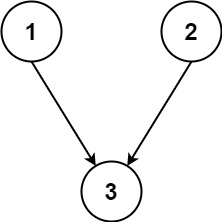
\includegraphics[width=0.15\linewidth]{images/lc1136_eg1}
\label{fig:lc1136eg1}
\end{figure}
\item Example 2: {\colorbox{CodeBackground}{\lstinline|n = 3, relations = [[1,2],[2,3],[3,1]] --> -1|}}
\begin{figure}[H]
\centering
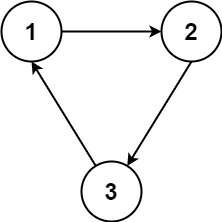
\includegraphics[width=0.15\linewidth]{images/lc1136_eg2}
\label{fig:lc1136eg2}
\end{figure}
\end{itemize}

\section{LC 1494 - Parallel Courses II}\label{lc1494}
{\hyperref[sec:topological_sort]{[Topological Sort]}}\\

You are given an integer {\colorbox{CodeBackground}{\lstinline|n|}} ({\colorbox{CodeBackground}{\lstinline|n >= 1|}}), which indicates that there are {\colorbox{CodeBackground}{\lstinline|n|}} courses labeled from {\colorbox{CodeBackground}{\lstinline|1|}} to {\colorbox{CodeBackground}{\lstinline|n|}}. You are also given an array relations where {\colorbox{CodeBackground}{\lstinline|relations[i] = [prevCourse_i, nextCourse_i]|}}, representing a prerequisite relationship between course {\colorbox{CodeBackground}{\lstinline|prevCourse_i|}} and course {\colorbox{CodeBackground}{\lstinline|nextCourse_i|}}: course {\colorbox{CodeBackground}{\lstinline|prevCourse_i|}} has to be taken before course {\colorbox{CodeBackground}{\lstinline|nextCourse_i|}}.\\

In one semester, you can take at most {\colorbox{CodeBackground}{\lstinline|k|}} ({\colorbox{CodeBackground}{\lstinline|k >= 1|}}) courses as long as you have taken all the prerequisites in the previous semesters for the courses you are taking.\\

Return the minimum number of semesters needed to take all courses.\\

Note: The test cases are generated such that it is possible to complete every course (i.e., the graph is a directed acyclic graph).

\begin{itemize}
\item {\colorbox{CodeBackground}{\lstinline|n = 4, relations = [[2,1],[3,1],[1,4]], k = 2 --> 3|}}
\begin{figure}[H]
\centering
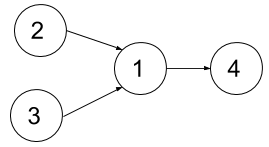
\includegraphics[width=0.3\linewidth]{images/lc1494_eg1}
\end{figure}
\item {\colorbox{CodeBackground}{\lstinline|n = 5, relations = [[2,1],[3,1],[4,1],[1,5]], k = 2 --> 4|}}
\begin{figure}[H]
\centering
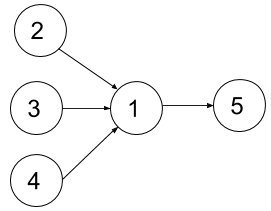
\includegraphics[width=0.3\linewidth]{images/lc1494_eg2}
\end{figure}
\end{itemize}

\section{LC 2050 - Parallel Courses III}\label{lc2050}
{\hyperref[sec:topological_sort]{[Topological Sort]}}\\

You are given an integer {\colorbox{CodeBackground}{\lstinline|n|}} ({\colorbox{CodeBackground}{\lstinline|n >= 1|}}), which indicates that there are {\colorbox{CodeBackground}{\lstinline|n|}} courses labeled from {\colorbox{CodeBackground}{\lstinline|1|}} to {\colorbox{CodeBackground}{\lstinline|n|}}. You are also given an array relations where {\colorbox{CodeBackground}{\lstinline|relations[i] = [prevCourse_i, nextCourse_i]|}}, representing a prerequisite relationship between course {\colorbox{CodeBackground}{\lstinline|prevCourse_i|}} and course {\colorbox{CodeBackground}{\lstinline|nextCourse_i|}}: course {\colorbox{CodeBackground}{\lstinline|prevCourse_i|}} has to be taken before course {\colorbox{CodeBackground}{\lstinline|nextCourse_i|}}.\\

Furthermore, you are given a {\colorbox{CodeBackground}{\lstinline|0|}}-indexed integer array {\colorbox{CodeBackground}{\lstinline|time|}} where {\colorbox{CodeBackground}{\lstinline|time[i]|}} denotes how many months it takes to complete the {\colorbox{CodeBackground}{\lstinline|(i+1)|}}th course.\\

You must find the minimum number of months needed to complete all the courses following these rules:
\begin{itemize}
\item You may start taking a course at any time if the prerequisites are met.
\item Any number of courses can be taken at the same time.
\end{itemize}

Return the minimum number of months needed to complete all the courses.\\

Note: The test cases are generated such that it is possible to complete every course (i.e., the graph is a directed acyclic graph).

\section{LC 0909 - Snakes and Ladders}
You are given an {\colorbox{CodeBackground}{\lstinline|n x n|}} integer matrix {\colorbox{CodeBackground}{\lstinline|board|}} where the cells are labeled from {\colorbox{CodeBackground}{\lstinline|1|}} to {\colorbox{CodeBackground}{\lstinline|n^2|}} in a \ul{Boustrophedon style} starting from the bottom left of the board (i.e. {\colorbox{CodeBackground}{\lstinline|board[n - 1][0]|}}) and alternating direction each row.\\

You start on square {\colorbox{CodeBackground}{\lstinline|1|}} of the board. In each move, starting from square {\colorbox{CodeBackground}{\lstinline|curr|}}, do the following:
\begin{itemize}
	\item Choose a destination square {\colorbox{CodeBackground}{\lstinline|next|}} with a label in the range {\colorbox{CodeBackground}{\lstinline|[curr + 1, min(curr + 6, n2)]|}}. This choice simulates the result of a standard {\colorbox{CodeBackground}{\lstinline|6|}}-sided die roll: i.e., there are at most {\colorbox{CodeBackground}{\lstinline|6|}} destinations, regardless of the size of the board.
	\item If {\colorbox{CodeBackground}{\lstinline|next|}} has a \ul{snake} or \ul{ladder}, you must move to the destination of that snake or ladder. Otherwise, you move to {\colorbox{CodeBackground}{\lstinline|next|}}. A board square on row {\colorbox{CodeBackground}{\lstinline|r|}} and column {\colorbox{CodeBackground}{\lstinline|c|}} has a snake or ladder if {\colorbox{CodeBackground}{\lstinline|board[r][c] != -1|}}. The destination of that snake or ladder is {\colorbox{CodeBackground}{\lstinline|board[r][c]|}}.
	\item The game ends when you reach the square {\colorbox{CodeBackground}{\lstinline|n^2|}}.
\end{itemize}

Note that:
\begin{itemize}
	\item  Squares {\colorbox{CodeBackground}{\lstinline|1|}} and {\colorbox{CodeBackground}{\lstinline|n^2|}} do not have a snake or ladder.
	\item You only take a snake or ladder at most once per move. If the destination to a snake or ladder is the start of another snake or ladder, you do not follow the subsequent snake or ladder.
\end{itemize}

Return the least number of moves required to reach the square {\colorbox{CodeBackground}{\lstinline|n^2|}}. If it is not possible to reach the square, return {\colorbox{CodeBackground}{\lstinline|-1|}}.\\

Example:
\begin{lstlisting}
board = [
[-1,-1,-1,-1,-1,-1],
[-1,-1,-1,-1,-1,-1],
[-1,-1,-1,-1,-1,-1],
[-1,35,-1,-1,13,-1],
[-1,-1,-1,-1,-1,-1],
[-1,15,-1,-1,-1,-1]] --> 4
\end{lstlisting}

\begin{figure}[H]
	\centering
	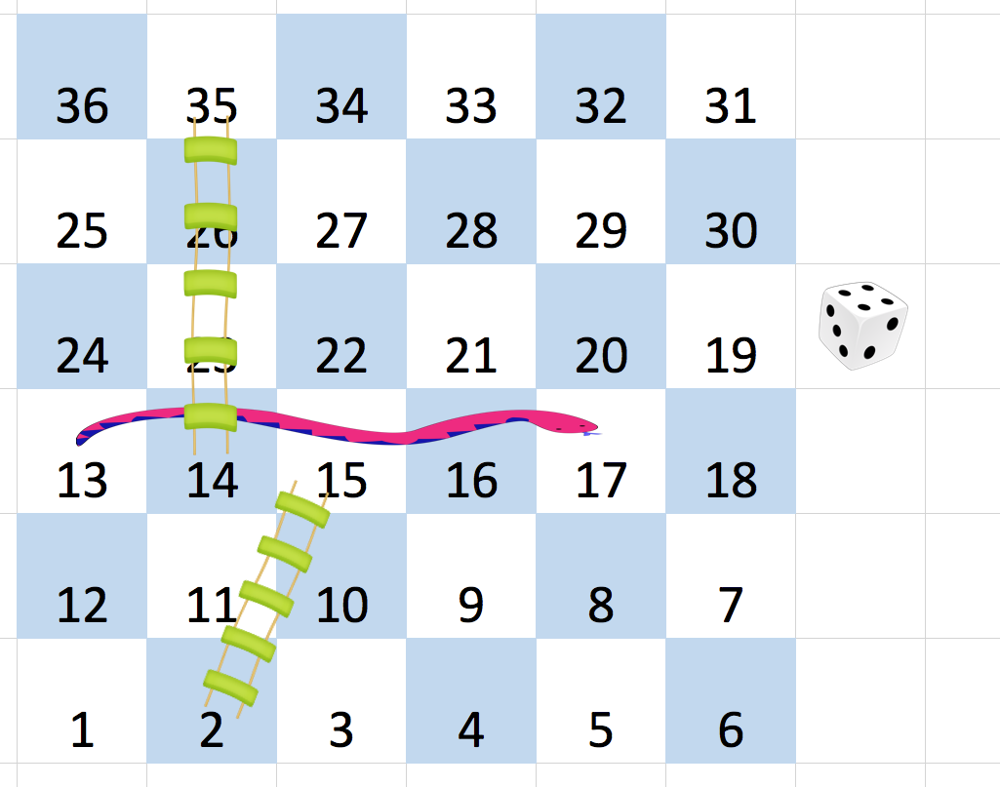
\includegraphics[width=0.4\linewidth]{images/lc0909_example}
	\label{fig:lc0909example}
\end{figure}

\subsection*{Solution}

\section{LC 0841 - Keys and Rooms}
There are {\colorbox{CodeBackground}{\lstinline|n|}} rooms labeled from {\colorbox{CodeBackground}{\lstinline|0|}} to {\colorbox{CodeBackground}{\lstinline|n - 1|}} and all the rooms are locked except for room {\colorbox{CodeBackground}{\lstinline|0|}}. Your goal is to visit all the rooms. However, you cannot enter a locked room without having its key.\\

When you visit a room, you may find a set of distinct keys in it. Each key has a number on it, denoting which room it unlocks, and you can take all of them with you to unlock the other rooms.\\

Given an array {\colorbox{CodeBackground}{\lstinline|rooms|}} where {\colorbox{CodeBackground}{\lstinline|rooms[i]|}} is the set of keys that you can obtain if you visited room {\colorbox{CodeBackground}{\lstinline|i|}}, return {\colorbox{CodeBackground}{\lstinline|true|}} if you can visit all the rooms, or {\colorbox{CodeBackground}{\lstinline|false|}} otherwise.\\

Examples:
\begin{itemize}
	\item {\colorbox{CodeBackground}{\lstinline|rooms = [[1],[2],[3],[]] --> true|}}
	\item {\colorbox{CodeBackground}{\lstinline|rooms = [[1,3],[3,0,1],[2],[0]] --> false|}}
\end{itemize}

\subsection*{Solution}
\begin{lstlisting}
bool canVisitAllRooms(std::vector<std::vector<int>>& rooms) {
	std::stack<int> dfs;                             // Stack to hold keys/rooms to visit.
	dfs.push(0);                                     // Start with room 0.
	std::vector<bool> visited(rooms.size(), false);  // Keep track of visited rooms.
	visited[0] = true;                               // Mark room 0 as visited.
	
	while (!dfs.empty()) {
		int currentRoom = dfs.top();
		dfs.pop();
		for (int key : rooms[currentRoom]) {
			if (!visited[key]) {    // If we haven't visited this room yet.
				visited[key] = true;  // Mark as visited.
				dfs.push(key);        // Add the room to the stack.
			}
		}
	}
	
	// Check if all rooms have been visited.
	for (bool room : visited) {
		if (!room) return false;
	}
	return true;
}
\end{lstlisting}

\section{LC 0847 - Shortest Path Visiting All Nodes}
You have an \ul{undirected, connected graph} of {\colorbox{CodeBackground}{\lstinline|n|}} ({\colorbox{CodeBackground}{\lstinline|n >= 1|}}) nodes labeled from {\colorbox{CodeBackground}{\lstinline|0|}} to {\colorbox{CodeBackground}{\lstinline|n - 1|}}. \\

You are given an array graph where {\colorbox{CodeBackground}{\lstinline|graph[i]|}} is a list of all the nodes connected with node {\colorbox{CodeBackground}{\lstinline|i|}} by an edge.\\

Return the length of the shortest path that visits every node. \\

You may start and stop at any node, you may revisit nodes multiple times, and you may reuse edges.

\begin{itemize}
\item Example 1: {\colorbox{CodeBackground}{\lstinline|graph = [[1,2,3],[0],[0],[0]] --> 4|}}
\begin{figure}[H]
\centering
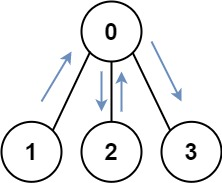
\includegraphics[width=0.18\linewidth]{images/lc0847_eg1}
\label{fig:lc0847eg1}
\end{figure}
One possible path is {\colorbox{CodeBackground}{\lstinline|[1,0,2,0,3]|}}
\item Example 2: {\colorbox{CodeBackground}{\lstinline|graph = [[1],[0,2,4],[1,3,4],[2],[1,2]] --> 4|}}
\begin{figure}[H]
\centering
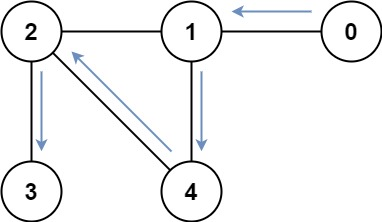
\includegraphics[width=0.3\linewidth]{images/lc0847_eg2}
\label{fig:lc0847eg2}
\end{figure}
One possible path is {\colorbox{CodeBackground}{\lstinline|[0,1,4,2,3]|}}
\end{itemize}

\subsection*{Solution - BFS}
\begin{lstlisting}
int shortestPathLength(std::vector<std::vector<int>>& graph) {
  int n = graph.size();
  std::vector<std::vector<bool>> visited(n, std::vector<bool>(1 << n, false));
  // tuple = {node, visited state, path length}
  std::queue<std::tuple<int, int, int>> q;
  for (int i = 0; i < n; ++i) {
    q.push({i, 1 << i, 1});
    visited[i][1 << i] = true;
  }
  while (!q.empty()) {
    auto [node, state, path_len] = q.front();
    q.pop();
    // all nodes are visited
    if (state == (1 << n) - 1) { return path_len - 1; }
    for (int neighbor : graph[node]) {
      int next_state = state | (1 << neighbor);
      if (!visited[neighbor][next_state]) {
        visited[neighbor][next_state] = true;
        q.push({neighbor, next_state, path_len + 1});
      }
    }
  }
  return -1;
}
\end{lstlisting}

\section{LC 2115 - Find All Possible Recipes from Given Supplies}\label{lc2115}
You have information about {\colorbox{CodeBackground}{\lstinline|n|}} ({\colorbox{CodeBackground}{\lstinline|n >= 1|}}) different recipes, and you are given a string array {\colorbox{CodeBackground}{\lstinline|recipes|}} and a 2D string array {\colorbox{CodeBackground}{\lstinline|ingredients|}}. The {\colorbox{CodeBackground}{\lstinline|i|}}th recipe has the name {\colorbox{CodeBackground}{\lstinline|recipes[i]|}}, and you can create it if you have all the needed ingredients from {\colorbox{CodeBackground}{\lstinline|ingredients[i]|}}. \\

Note that:
\begin{itemize}
\item Ingredients to a recipe may need to be created from other recipes, i.e., {\colorbox{CodeBackground}{\lstinline|ingredients[i]|}} may contain a string that is in {\colorbox{CodeBackground}{\lstinline|recipes|}}.
\item Two recipes may contain each other in their ingredients.
\end{itemize}

You are also given a string array {\colorbox{CodeBackground}{\lstinline|supplies|}} containing all the ingredients that you initially have, and you have an infinite supply of all of them.\\

Return a list of all the recipes that you can create. You may return the answer in any order.\\

\begin{itemize}
\item Example 1:
\begin{lstlisting}
recipes = ["bread"]
ingredients = [["yeast","flour"]]
supplies = ["yeast","flour","corn"]
--> ["bread"]
\end{lstlisting}
We can create "bread" since we have the ingredients "yeast" and "flour".
\item Example 2:
\begin{lstlisting}
recipes = ["bread","sandwich"]
ingredients = [["yeast","flour"],["bread","meat"]]
supplies = ["yeast","flour","meat"]
--> ["bread","sandwich"]
\end{lstlisting}
We can create "bread" since we have the ingredients "yeast" and "flour".\\
We can create "sandwich" since we have the ingredient "meat" and can create the ingredient "bread".
\item Example 3:
\begin{lstlisting}
recipes = ["bread","sandwich","burger"]
ingredients = [["yeast","flour"],["bread","meat"],["sandwich","meat","bread"]]
supplies = ["yeast","flour","meat"]
--> ["bread","sandwich","burger"]
\end{lstlisting}
We can create "bread" since we have the ingredients "yeast" and "flour".\\
We can create "sandwich" since we have the ingredient "meat" and can create the ingredient "bread".\\
We can create "burger" since we have the ingredient "meat" and can create the ingredients "bread" and "sandwich".
\end{itemize}

\section{LC 2101 - Detonate the Maximum Bombs}
You are given a list of bombs. The range of a bomb is defined as the area where its effect can be felt. This area is in the shape of a circle with the center as the location of the bomb.\\

The bombs are represented by a {\colorbox{CodeBackground}{\lstinline|0|}}-indexed 2D integer array {\colorbox{CodeBackground}{\lstinline|bombs|}} where {\colorbox{CodeBackground}{\lstinline|bombs[i] = [x_i, y_i, r_i]|}}. {\colorbox{CodeBackground}{\lstinline|x_i|}} and {\colorbox{CodeBackground}{\lstinline|y_i|}} denote the X-coordinate and Y-coordinate of the location of the {\colorbox{CodeBackground}{\lstinline|i|}}th bomb, whereas {\colorbox{CodeBackground}{\lstinline|r_i|}} denotes the radius of its range.\\

You may choose to detonate a single bomb. When a bomb is detonated, it will detonate all bombs that lie in its range. These bombs will further detonate the bombs that lie in their ranges.\\

Given the list of {\colorbox{CodeBackground}{\lstinline|bombs|}}, return the maximum number of bombs that can be detonated if you are allowed to detonate only one bomb.

\begin{itemize}
\item Example 1: {\colorbox{CodeBackground}{\lstinline|bombs = [[2,1,3],[6,1,4]] --> 2|}}
\begin{figure}[H]
\centering
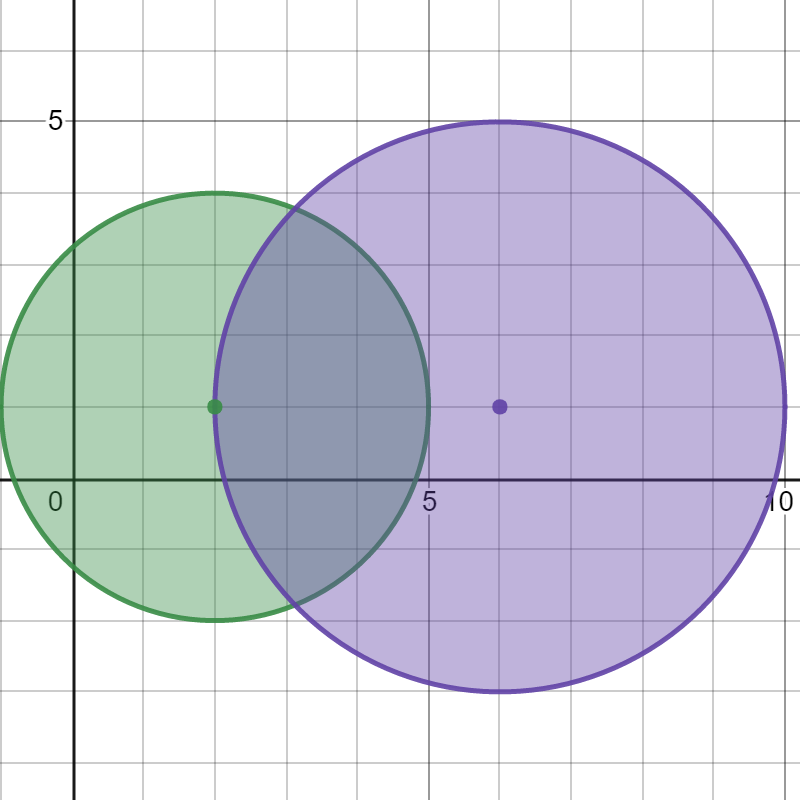
\includegraphics[width=0.3\linewidth]{images/lc2101_eg1}
\end{figure}
The above figure shows the positions and ranges of the {\colorbox{CodeBackground}{\lstinline|2|}} bombs.\\
If we detonate the left bomb, the right bomb will not be affected.\\
But if we detonate the right bomb, both bombs will be detonated.\\
So the maximum bombs that can be detonated is {\colorbox{CodeBackground}{\lstinline|max(1, 2) = 2|}}.
\item Example 2:
\begin{figure}[H]
\centering
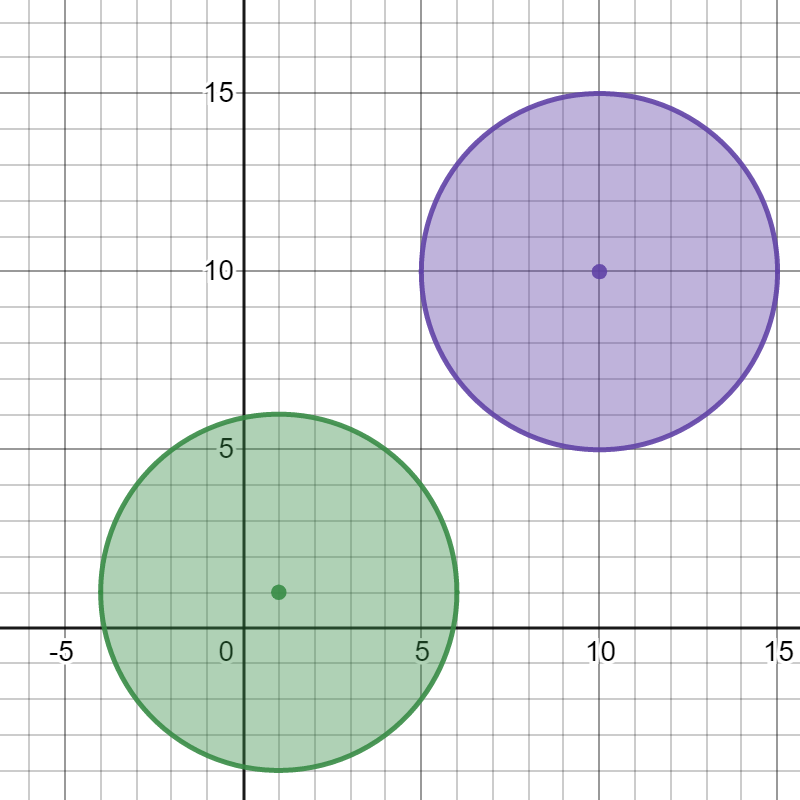
\includegraphics[width=0.3\linewidth]{images/lc2101_eg2}
\end{figure}
Detonating either bomb will not detonate the other bomb, so the maximum number of bombs that can be detonated is {\colorbox{CodeBackground}{\lstinline|1|}}.
\item Example 3:
\begin{figure}[H]
\centering
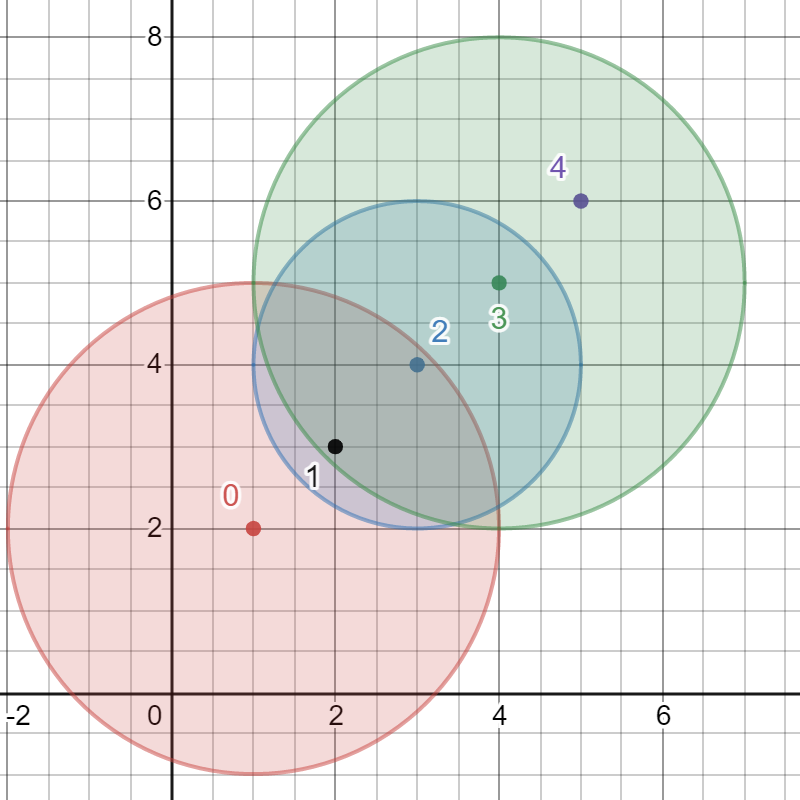
\includegraphics[width=0.3\linewidth]{images/lc2101_eg3}
\end{figure}
The best bomb to detonate is bomb {\colorbox{CodeBackground}{\lstinline|0|}} because:\\
- Bomb {\colorbox{CodeBackground}{\lstinline|0|}} detonates bombs {\colorbox{CodeBackground}{\lstinline|1|}} and {\colorbox{CodeBackground}{\lstinline|2|}}. The red circle denotes the range of bomb {\colorbox{CodeBackground}{\lstinline|0|}}.\\
- Bomb {\colorbox{CodeBackground}{\lstinline|2|}} detonates bomb {\colorbox{CodeBackground}{\lstinline|3|}}. The blue circle denotes the range of bomb {\colorbox{CodeBackground}{\lstinline|2|}}.\\
- Bomb {\colorbox{CodeBackground}{\lstinline|3|}} detonates bomb {\colorbox{CodeBackground}{\lstinline|4|}}. The green circle denotes the range of bomb {\colorbox{CodeBackground}{\lstinline|3|}}.\\
Thus all {\colorbox{CodeBackground}{\lstinline|5|}} bombs are detonated.
\end{itemize}


\section{LC 1584 - Min Cost to Connect All Points}
You are given a \ul{non-empty} array {\colorbox{CodeBackground}{\lstinline|points|}} representing integer coordinates of some points on a 2D-plane, where {\colorbox{CodeBackground}{\lstinline|points[i] = [x_i, y_i]|}}.\\

The cost of connecting two points {\colorbox{CodeBackground}{\lstinline|[xi, yi]|}} and {\colorbox{CodeBackground}{\lstinline|[xj, yj]|}} is the manhattan distance between them: {\colorbox{CodeBackground}{\lstinline|\|x_i - x_j\| + \|y_i - yj_\||}}, where {\colorbox{CodeBackground}{\lstinline|\|val\||}} denotes the absolute value of val.\\

Return the minimum cost to make all points connected. All points are connected if there is exactly one simple path between any two points.

\begin{itemize}
\item {\colorbox{CodeBackground}{\lstinline|points = [[0,0],[2,2],[3,10],[5,2],[7,0]] --> 20|}}
\begin{figure}[H]
\centering
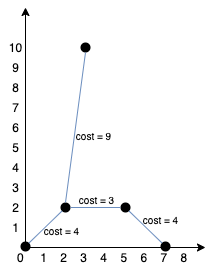
\includegraphics[width=0.25\linewidth]{images/lc1584_eg}
\label{fig:lc1584eg}
\item {\colorbox{CodeBackground}{\lstinline|points = [[3,12],[-2,5],[-4,1]] --> 18|}}
\end{figure}
\end{itemize}

\section{LC 2858 - Minimum Edge Reversals So Every Node Is Reachable}
There is a \ul{simple directed graph} with {\colorbox{CodeBackground}{\lstinline|n|}} nodes labeled from {\colorbox{CodeBackground}{\lstinline|0|}} to {\colorbox{CodeBackground}{\lstinline|n - 1|}}. The graph would form a tree if its edges were bi-directional.\\

You are given an integer {\colorbox{CodeBackground}{\lstinline|n|}} ({\colorbox{CodeBackground}{\lstinline|n >= 2|}}) and a 2D integer array {\colorbox{CodeBackground}{\lstinline|edges|}}, where {\colorbox{CodeBackground}{\lstinline|edges[i] = [u_i, v_i]|}} represents a \ul{directed edge} going from node {\colorbox{CodeBackground}{\lstinline|u_i|}} to node {\colorbox{CodeBackground}{\lstinline|v_i|}}.\\

An edge reversal changes the direction of an edge, i.e., a directed edge going from node {\colorbox{CodeBackground}{\lstinline|u_i|}} to node {\colorbox{CodeBackground}{\lstinline|v_i|}} becomes a directed edge going from node {\colorbox{CodeBackground}{\lstinline|v_i|}} to node {\colorbox{CodeBackground}{\lstinline|u_i|}}.\\

For every node {\colorbox{CodeBackground}{\lstinline|i|}} in the range {\colorbox{CodeBackground}{\lstinline|[0, n - 1]|}}, your task is to independently calculate the minimum number of edge reversals required so it is possible to reach any other node starting from node {\colorbox{CodeBackground}{\lstinline|i|}} through a sequence of directed edges.\\

Return an integer array {\colorbox{CodeBackground}{\lstinline|answer|}}, where {\colorbox{CodeBackground}{\lstinline|answer[i]|}} is the minimum number of edge reversals required so it is possible to reach any other node starting from node {\colorbox{CodeBackground}{\lstinline|i|}} through a sequence of directed edges.

\begin{itemize}
\item Example 1: {\colorbox{CodeBackground}{\lstinline|n = 4, edges = [[2,0],[2,1],[1,3]] --> [1,1,0,2]|}}
\begin{figure}[H]
\centering
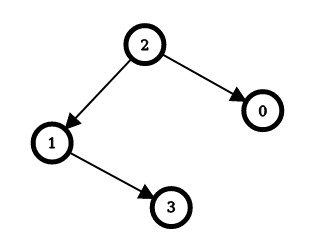
\includegraphics[width=0.3\linewidth]{images/lc2858_eg1}
\label{fig:lc2858eg1}
\end{figure}
The image above shows the graph formed by the edges.\\
For node {\colorbox{CodeBackground}{\lstinline|0|}}: after reversing the edge {\colorbox{CodeBackground}{\lstinline|[2,0]|}}, it is possible to reach any other node starting from node {\colorbox{CodeBackground}{\lstinline|0|}}.\\
So, {\colorbox{CodeBackground}{\lstinline|answer[0] = 1|}}.\\
For node {\colorbox{CodeBackground}{\lstinline|1|}}: after reversing the edge {\colorbox{CodeBackground}{\lstinline|[2,1]|}}, it is possible to reach any other node starting from node {\colorbox{CodeBackground}{\lstinline|1|}}.\\
So, {\colorbox{CodeBackground}{\lstinline|answer[1] = 1|}}.\\
For node {\colorbox{CodeBackground}{\lstinline|2|}}: it is already possible to reach any other node starting from node {\colorbox{CodeBackground}{\lstinline|2|}}.\\
So, {\colorbox{CodeBackground}{\lstinline|answer[2] = 0|}}.\\
For node {\colorbox{CodeBackground}{\lstinline|3|}}: after reversing the edges {\colorbox{CodeBackground}{\lstinline|[1,3]|}} and {\colorbox{CodeBackground}{\lstinline|[2,1]|}}, it is possible to reach any other node starting from node {\colorbox{CodeBackground}{\lstinline|3|}}.\\
So, {\colorbox{CodeBackground}{\lstinline|answer[3] = 2|}}.
\item Example 2: {\colorbox{CodeBackground}{\lstinline|n = 3, edges = [[1,2],[2,0]] --> [2,0,1]|}}
\begin{figure}[H]
\centering
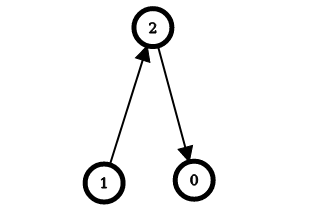
\includegraphics[width=0.3\linewidth]{images/lc2858_eg2}
\label{fig:lc2858eg2}
\end{figure}
The image above shows the graph formed by the edges.\\
For node {\colorbox{CodeBackground}{\lstinline|0|}}: after reversing the edges {\colorbox{CodeBackground}{\lstinline|[2,0]|}} and {\colorbox{CodeBackground}{\lstinline|[1,2]|}}, it is possible to reach any other node starting from node {\colorbox{CodeBackground}{\lstinline|0|}}.\\
So, {\colorbox{CodeBackground}{\lstinline|answer[0] = 2|}}.\\
For node {\colorbox{CodeBackground}{\lstinline|1|}}: it is already possible to reach any other node starting from node {\colorbox{CodeBackground}{\lstinline|1|}}.\\
So, {\colorbox{CodeBackground}{\lstinline|answer[1] = 0|}}.\\
For node {\colorbox{CodeBackground}{\lstinline|2|}}: after reversing the edge {\colorbox{CodeBackground}{\lstinline|[1, 2]|}}, it is possible to reach any other node starting from node {\colorbox{CodeBackground}{\lstinline|2|}}.\\
So, {\colorbox{CodeBackground}{\lstinline|answer[2] = 1|}}.
\end{itemize}

\section{LC 0547 - Number of Provinces}
There are {\colorbox{CodeBackground}{\lstinline|n|}} ({\colorbox{CodeBackground}{\lstinline|n >= 1|}}) cities. Some of them are connected, while some are not. If city {\colorbox{CodeBackground}{\lstinline|a|}} is connected directly with city {\colorbox{CodeBackground}{\lstinline|b|}}, and city {\colorbox{CodeBackground}{\lstinline|b|}} is connected directly with city {\colorbox{CodeBackground}{\lstinline|c|}}, then city {\colorbox{CodeBackground}{\lstinline|a|}} is connected indirectly with city {\colorbox{CodeBackground}{\lstinline|c|}}.\\

A \ul{province} is a group of directly or indirectly connected cities and no other cities outside of the group.\\

You are given an {\colorbox{CodeBackground}{\lstinline|n x n|}} matrix {\colorbox{CodeBackground}{\lstinline|isConnected|}} where {\colorbox{CodeBackground}{\lstinline|isConnected[i][j] = 1|}} if the {\colorbox{CodeBackground}{\lstinline|i|}}th city and the {\colorbox{CodeBackground}{\lstinline|j|}}th city are directly connected, and {\colorbox{CodeBackground}{\lstinline|isConnected[i][j] = 0|}} otherwise. Note that {\colorbox{CodeBackground}{\lstinline|isConnected[i][j] == isConnected[j][i]|}}.

Return the total number of provinces.

\begin{itemize}
\item {\colorbox{CodeBackground}{\lstinline|isConnected = [[1,1,0],[1,1,0],[0,0,1]] --> 2|}}
\begin{figure}[H]
\centering
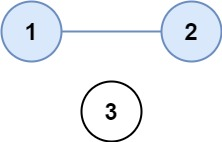
\includegraphics[width=0.15\linewidth]{images/lc0547_eg1}
\end{figure}
\item {\colorbox{CodeBackground}{\lstinline|isConnected = [[1,0,0],[0,1,0],[0,0,1]] --> 3|}}
\begin{figure}[H]
\centering
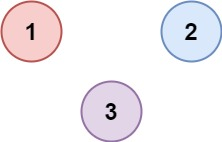
\includegraphics[width=0.15\linewidth]{images/lc0547_eg2}
\end{figure}
\end{itemize}

\section{LC 0797 - All Paths From Source to Target}
Given a \ul{directed acyclic graph (DAG)} of {\colorbox{CodeBackground}{\lstinline|n|}} ({\colorbox{CodeBackground}{\lstinline|n >= 2|}}) nodes labeled from {\colorbox{CodeBackground}{\lstinline|0|}} to {\colorbox{CodeBackground}{\lstinline|n - 1|}}, find all possible paths from node {\colorbox{CodeBackground}{\lstinline|0|}} to node {\colorbox{CodeBackground}{\lstinline|n - 1|}} and return them in any order.\\

The graph is given as follows: {\colorbox{CodeBackground}{\lstinline|graph[i]|}} is a list of all nodes you can visit from node {\colorbox{CodeBackground}{\lstinline|i|}} (i.e., there is a directed edge from node {\colorbox{CodeBackground}{\lstinline|i|}} to node {\colorbox{CodeBackground}{\lstinline|graph[i][j]|}}).

\begin{itemize}
\item {\colorbox{CodeBackground}{\lstinline|graph = [[1,2],[3],[3],[]] --> [[0,1,3],[0,2,3]]|}}
\begin{figure}[H]
\centering
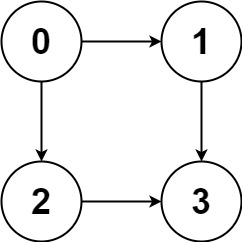
\includegraphics[width=0.15\linewidth]{images/lc0797_eg1}
\end{figure}
\item {\colorbox{CodeBackground}{\lstinline|graph = [[4,3,1],[3,2,4],[3],[4],[]] --> [[0,4],[0,3,4],[0,1,3,4],[0,1,2,3,4],[0,1,4]]|}}
\begin{figure}[H]
\centering
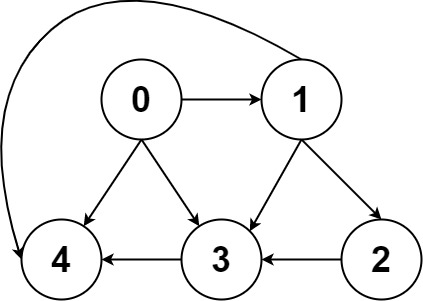
\includegraphics[width=0.28\linewidth]{images/lc0797_eg2}
\end{figure}
\end{itemize}
\chapter{Matrix}
\section{LC 0200 - Number of Islands}
Given an {\colorbox{CodeBackground}{\lstinline|m x n|}} binary grid {\colorbox{CodeBackground}{\lstinline|grid|}} which represents a map of {\colorbox{CodeBackground}{\lstinline|'1'|}}s (\ul{land}) and {\colorbox{CodeBackground}{\lstinline|'0'|}}s (\ul{water}), return the number of \ul{islands}.\\

An \ul{island} is surrounded by water and is formed by connecting adjacent lands horizontally or vertically. \\

You may assume all four edges of {\colorbox{CodeBackground}{\lstinline|grid|}} are all surrounded by water.\\

\begin{itemize}
\item Example 1
\begin{lstlisting}
[["1","1","1","1","0"],
 ["1","1","0","1","0"],
 ["1","1","0","0","0"],
 ["0","0","0","0","0"]] --> 1
\end{lstlisting}
\item Example 2
\begin{lstlisting}
[["1","1","0","0","0"],
 ["1","1","0","0","0"],
 ["0","0","1","0","0"],
 ["0","0","0","1","1"]] --> 3
\end{lstlisting}
\end{itemize}

\subsection*{Solution 1 - DFS}
\begin{lstlisting}
int numIslands(std::vector<std::vector<char>>& grid) {
  int num_island = 0;
  for (int i = 0; i < grid.size(); ++i) {
    for (int j = 0; j < grid[0].size(); ++j) {
      if (grid[i][j] == '1') {
        DFSSinkLand(grid, i, j);
        ++num_island;
      }
    }
  }
  return num_island;
}

void DFSSinkLand(std::vector<std::vector<char>>& grid, int i, int j) {
  if (i < 0 || i >= grid.size() || j < 0 || j >= grid[0].size()) { return; }
  if (grid[i][j] == '0') { return; }
  grid[i][j] = '0';
  DFSSinkLand(grid, i - 1, j);
  DFSSinkLand(grid, i + 1, j);
  DFSSinkLand(grid, i, j - 1);
  DFSSinkLand(grid, i, j + 1);
}
\end{lstlisting}

\subsection*{Solution 2 - BFS}
\begin{lstlisting}
int numIslands(std::vector<std::vector<char>>& grid) {
  if (grid.empty()) { return 0; }
  int num_island = 0;
  for (int i = 0; i < grid.size(); ++i) {
    for (int j = 0; j < grid[0].size(); ++j) {
      if (grid[i][j] == '1') {
        BFS(grid, i, j);
        ++num_island;
      }
    }
  }
  return num_island;
}

void BFS(std::vector<std::vector<char>>& grid, int i, int j) {
  std::queue<std::pair<int, int>> q;
  q.emplace(i, j);
  grid[i][j] = '0';
  std::vector<std::pair<int, int>> dirs = {{-1, 0}, {1, 0}, {0, -1}, {0, 1}};
  while (!q.empty()) {
    auto [r, c] = q.front();
    q.pop();
    for (auto [dr, dc] : dirs) {
      int new_r = r + dr;
      int new_c = c + dc;
      if (new_r >= 0 && new_r < grid.size() && new_c >= 0 && new_c < grid[0].size()
          && grid[new_r][new_c] == '1') {
        q.emplace(new_r, new_c);
        grid[new_r][new_c] = '0';
      }
    }
  }
}
\end{lstlisting}

\subsection*{Solution 3 - BFS (Time Limit Exceeded)}
The only difference between Solution 2 and Solution 3 lies in the timing of sinking a land cell.
\begin{itemize}
\item Solution 2 sinks the neighboring land cells before enqueuing them.
\item Solution 3 delays this sinking until after the land cell is dequeued.
\end{itemize}

This state of cells influences whether or not BFS decides to explore the neighboring cells. A smart choice it to update those states as early as we can. If we wait too long to sink lands, we might end up enqueuing duplicate land cells again and again, which, in the best-case scenario, reduces the algorithm's speed and, in the worst-case scenario, leads to an infinite loop.\\

See the more general form of this issue here: \hyperref[subsubsec:graph_universal_implementation_bfs]{Graph (Universal Implementation) - BFS}.

\begin{lstlisting}
int numIslands(std::vector<std::vector<char>>& grid) {
  if (grid.empty()) { return 0; }
  int num_island = 0;
  for (int i = 0; i < grid.size(); ++i) {
    for (int j = 0; j < grid[0].size(); ++j) {
      if (grid[i][j] == '1') {
        BFSSinkLand(grid, i, j);
        ++num_island;
      }
    }
  }
  return num_island;
}

void BFSSinkLand(std::vector<std::vector<char>>& grid, int i, int j) {
  std::queue<std::pair<int, int>> q;
  q.emplace(i, j);
  grid[i][j] = '0';
  std::vector<std::pair<int, int>> dirs = {{-1, 0}, {1, 0}, {0, -1}, {0, 1}};
  while (!q.empty()) {
    auto [r, c] = q.front();
    q.pop();
    grid[r][c] = '0';
    for (auto [dr, dc] : dirs) {
      int new_r = r + dr;
      int new_c = c + dc;
      if (new_r >= 0 && new_r < grid.size() && new_c >= 0 && new_c < grid[0].size()
          && grid[new_r][new_c] == '1') {
        q.emplace(new_r, new_c);
      }
    }
  }
}
\end{lstlisting}

\section{LC 1020 - Number of Enclaves}
You are given an {\colorbox{CodeBackground}{\lstinline|m x n|}} binary matrix {\colorbox{CodeBackground}{\lstinline|grid|}}, where {\colorbox{CodeBackground}{\lstinline|0|}} represents a \ul{sea cell} and {\colorbox{CodeBackground}{\lstinline|1|}} represents a \ul{land cell}.\\

A \ul{move} consists of:
\begin{itemize}
\item walking from one \ul{land cell} to another adjacent ({\colorbox{CodeBackground}{\lstinline|4|}}-directionally) \ul{land cell}
\item or walking off the boundary of the {\colorbox{CodeBackground}{\lstinline|grid|}}.
\end{itemize}

Return the number of \ul{land cells} in {\colorbox{CodeBackground}{\lstinline|grid|}} for which we cannot walk off the boundary of the {\colorbox{CodeBackground}{\lstinline|grid|}} in any number of moves.\\

\begin{itemize}
	\item Example 1
\begin{lstlisting}
[[0,0,0,0],
 [1,0,1,0],
 [0,1,1,0],
 [0,0,0,0]] --> 3
\end{lstlisting}
	\begin{figure}[H]
		\centering
		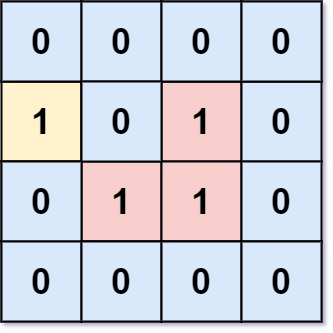
\includegraphics[width=0.2\linewidth]{images/lc1020_eg1}
		\label{fig:lc1020eg1}
	\end{figure}
	\item Example 2
\begin{lstlisting}
[[0,1,1,0],
 [0,0,1,0],
 [0,0,1,0],
 [0,0,0,0]] --> 0
\end{lstlisting}
	\begin{figure}[H]
		\centering
		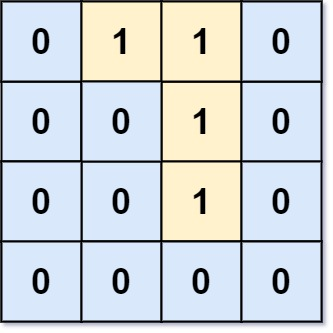
\includegraphics[width=0.2\linewidth]{images/lc1020_eg2}
		\label{fig:lc1020eg2}
	\end{figure}
\end{itemize}

\subsection*{Solution 1 - DFS}
\begin{lstlisting}
int numEnclaves(std::vector<std::vector<int>>& grid) {
  int m = grid.size();
  int n = grid[0].size();
  for (int i = 0; i < m; ++i) {
    DFSSinkLand(grid, i, 0);
    DFSSinkLand(grid, i, n - 1);
  }
  for (int j = 1; j < n - 1; ++j) {
    DFSSinkLand(grid, 0, j);
    DFSSinkLand(grid, m - 1, j);
  }
  int count = 0;
  for (int i = 1; i < m - 1; ++i) {
    for (int j = 1; j < n - 1; ++j) {
      if (grid[i][j] == 1) { ++count; }
    }
  }
  return count;
}

void DFSSinkLand(std::vector<std::vector<int>>& grid, int i, int j) {
  if (i < 0 || i >= grid.size() || j < 0 || j >= grid[0].size()) { return; }
  if (grid[i][j] == 0) { return; }
  grid[i][j] = 0;
  DFSSinkLand(grid, i - 1, j);
  DFSSinkLand(grid, i + 1, j);
  DFSSinkLand(grid, i, j - 1);
  DFSSinkLand(grid, i, j + 1);
}
\end{lstlisting}

\subsection*{Solution 2 - BFS}
\begin{lstlisting}
int numEnclaves(std::vector<std::vector<int>>& grid) {
  int m = grid.size();
  int n = grid[0].size();
  std::queue<std::pair<int, int>> q;
  for (int i = 0; i < m; ++i) {
    if (grid[i][0] == 1) { q.emplace(i, 0); }
    if (grid[i][n - 1] == 1) { q.emplace(i, n - 1); }
  }
  for (int j = 1; j < n - 1; ++j) {
    if (grid[0][j] == 1) { q.emplace(0, j); }
    if (grid[m - 1][j] == 1) { q.emplace(m - 1, j); }
  }
  std::vector<std::pair<int, int>> dirs = {{-1, 0}, {1, 0}, {0, -1}, {0, 1}};
  while (!q.empty()) {
    auto [r, c] = q.front();
    q.pop();
    for (auto [dr, dy] : dirs) {
      int new_r = r + dr;
      int new_c = c + dy;
      if (new_r >= 0 && new_r < m && new_c >= 0 && new_c < n && grid[new_r][new_c] == 1) {
        q.emplace(new_r, new_c);
        grid[new_r][new_c] = 0;
      }
    }
  }
  int count = 0;
  for (int i = 1; i < m - 1; ++i) {
    for (int j = 1; j < n - 1; ++j) {
      if (grid[i][j] == 1) { ++count; }
    }
  }
  return count;
}
\end{lstlisting}

\section{LC 0463 - Island Perimeter}
You are given {\colorbox{CodeBackground}{\lstinline|m x n|}} {\colorbox{CodeBackground}{\lstinline|grid|}} representing a map where {\colorbox{CodeBackground}{\lstinline|1|}} represents \ul{land} and {\colorbox{CodeBackground}{\lstinline|0|}} represents \ul{water}.\\

An \ul{island} is a group of {\colorbox{CodeBackground}{\lstinline|1|}}'s (representing land) connected {\colorbox{CodeBackground}{\lstinline|4|}}-directionally (horizontal or vertical). \\

You may assume all four edges of the {\colorbox{CodeBackground}{\lstinline|grid|}} are surrounded by water.\\

In this question, the island doesn't have "lakes", meaning the water inside isn't connected to the water around the island. And there is exactly one island in {\colorbox{CodeBackground}{\lstinline|grid|}}.\\

Determine the perimeter of the island.

\begin{itemize}
\item Example 1
\begin{lstlisting}
[[0,1,0,0],
 [1,1,1,0],
 [0,1,0,0],
 [1,1,0,0]] --> 16
\end{lstlisting}
\begin{figure}[H]
\centering
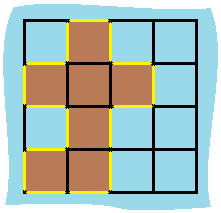
\includegraphics[width=0.2\linewidth]{images/lc0463_eg}
\label{fig:lc0463eg}
\end{figure}
\item Example 2
\begin{lstlisting}
grid = [[1]] --> 4
\end{lstlisting}
\item Example 3
\begin{lstlisting}
grid = [[1,0]] --> 4
\end{lstlisting}
\end{itemize}

\subsection*{Solution 1 - Brute Force}
\begin{lstlisting}
int islandPerimeter(std::vector<std::vector<int>>& grid) {
  int perimeter = 0;
  for (int i = 0; i < grid.size(); ++i) {
    for (int j = 0; j < grid[0].size(); ++j) {
      if (grid[i][j] == 1) {
        if (i == 0 || grid[i - 1][j] == 0) { perimeter++; }
        if (i == grid.size() - 1 || grid[i + 1][j] == 0) { perimeter++; }
        if (j == 0 || grid[i][j - 1] == 0) { perimeter++; }
        if (j == grid[0].size() - 1 || grid[i][j + 1] == 0) { perimeter++; }
      }
    }
  }
  return perimeter;
}
\end{lstlisting}

\subsection*{Solution 2 - Count Lands and Connections}
\begin{lstlisting}
int islandPerimeter(std::vector<std::vector<int>>& grid) {
  int num_lands = 0;
  int num_connections = 0;
  int m = grid.size();
  int n = grid[0].size();
  for (int i = 0; i < m; ++i) {
    for (int j = 0; j < n; ++j) {
      if (grid[i][j] == 1) {
        ++num_lands;
        if (j < n - 1 && grid[i][j + 1] == 1) { ++num_connections; }
        if (i < m - 1 && grid[i + 1][j] == 1) { ++num_connections; }
      }
    }
  }
  return 4 * num_lands - 2 * num_connections;
}
\end{lstlisting}

\section{LC 0130 - Surrounded Regions}
Given an {\colorbox{CodeBackground}{\lstinline|m x n|}} matrix {\colorbox{CodeBackground}{\lstinline|board|}} containing {\colorbox{CodeBackground}{\lstinline|'X'|}} and {\colorbox{CodeBackground}{\lstinline|'O'|}}, \ul{capture} all regions that are {\colorbox{CodeBackground}{\lstinline|4|}}-directionally surrounded by {\colorbox{CodeBackground}{\lstinline|'X'|}}. \\

A region is \ul{captured} by flipping all {\colorbox{CodeBackground}{\lstinline|'O'|}}s into {\colorbox{CodeBackground}{\lstinline|'X'|}}s in that surrounded region.

\begin{itemize}
\item Example 1
\begin{lstlisting}
[["X","X","X","X"],
 ["X","O","O","X"],
 ["X","X","O","X"],
 ["X","O","X","X"]]
--> 
[["X","X","X","X"],
 ["X","X","X","X"],
 ["X","X","X","X"],
 ["X","O","X","X"]]

\end{lstlisting}
\begin{figure}[H]
\centering
\includegraphics[width=0.4\linewidth]{images/lc0130_eg}
\label{fig:lc0130eg}
\end{figure}
\item Example 2
\begin{lstlisting}
[["X"]] --> [["X"]]
\end{lstlisting}
\end{itemize}

\subsection*{Solution - DFS}
\begin{lstlisting}
void solve(std::vector<std::vector<char>>& board) {
  int m = board.size();
  int n = board[0].size();
  // mark 'O's on border and connected to border as 'S' (safe)
  for (int i = 0; i < m; ++i) {
    if (board[i][0] == 'O') { DFSMarkSafe(board, i, 0); }
    if (board[i][n - 1] == 'O') { DFSMarkSafe(board, i, n - 1); }
  }
  for (int j = 0; j < n; ++j) {
    if (board[0][j] == 'O') { DFSMarkSafe(board, 0, j); }
    if (board[m - 1][j] == 'O') { DFSMarkSafe(board, m - 1, j); }
  }
  // flip 'O's to 'X's and 'S's back to 'O's
  for (int i = 0; i < m; ++i) {
    for (int j = 0; j < n; ++j) {
      if (board[i][j] == 'O') { board[i][j] = 'X'; }
      if (board[i][j] == 'S') { board[i][j] = 'O'; }
    }
  }
}

void DFSMarkSafe(std::vector<std::vector<char>>& board, int i, int j) {
  if (i < 0 || i >= board.size() || j < 0 || j >= board[0].size()) { return; }
  if (board[i][j] != 'O') { return; }
  board[i][j] = 'S';
  DFSMarkSafe(board, i - 1, j);
  DFSMarkSafe(board, i + 1, j);
  DFSMarkSafe(board, i, j - 1);
  DFSMarkSafe(board, i, j + 1);
}
\end{lstlisting}

\section{LC 0733 - Flood Fill}
An image is represented by an {\colorbox{CodeBackground}{\lstinline|m x n|}} integer grid {\colorbox{CodeBackground}{\lstinline|image|}} where {\colorbox{CodeBackground}{\lstinline|image[i][j]|}} represents the pixel value of the image.\\

You are also given three integers {\colorbox{CodeBackground}{\lstinline|sr|}}, {\colorbox{CodeBackground}{\lstinline|sc|}}, and {\colorbox{CodeBackground}{\lstinline|color|}}. You should perform a \ul{flood fill} on the image starting from the pixel {\colorbox{CodeBackground}{\lstinline|image[sr][sc]|}}.\\

To perform a \ul{flood fill}, consider:
\begin{enumerate}
\item the starting pixel;
\item plus any pixels connected {\colorbox{CodeBackground}{\lstinline|4|}}-directionally to the starting pixel of the same color as the starting pixel;
\item plus any pixels connected {\colorbox{CodeBackground}{\lstinline|4|}}-directionally to those pixels (also with the same color);
\item and so on.
\end{enumerate}
Replace the color of all of the aforementioned pixels with {\colorbox{CodeBackground}{\lstinline|color|}}.\\

Return the modified image after performing the \ul{flood fill}.\\

\begin{itemize}
\item Example 1
\begin{lstlisting}
image = 
[[1,1,1],
 [1,1,0],
 [1,0,1]]
sr = 1, sc = 1, color = 2
--> 
[[2,2,2],
 [2,2,0],
 [2,0,1]]
\end{lstlisting}
\begin{figure}[H]
\centering
\includegraphics[width=0.4\linewidth]{images/lc0733_eg}
\label{fig:lc0733eg}
\end{figure}
\item Example 2
\begin{lstlisting}
image = 
[[0,0,0],
 [0,0,0]]
sr = 0, sc = 0, color = 0
-->
[[0,0,0],
 [0,0,0]]
\end{lstlisting}
\end{itemize}

\subsection*{Solution - DFS}
\begin{lstlisting}
void dfs(std::vector<std::vector<int>>& image, int sr, int sc, int newColor, int oldColor) {
	if (sr < 0 || sc < 0 || sr >= image.size() || sc >= image[0].size()
	|| image[sr][sc] != oldColor) {
		return;
	}
	
	image[sr][sc] = newColor;
	
	// Flood fill in all 4 directions
	dfs(image, sr + 1, sc, newColor, oldColor);
	dfs(image, sr - 1, sc, newColor, oldColor);
	dfs(image, sr, sc + 1, newColor, oldColor);
	dfs(image, sr, sc - 1, newColor, oldColor);
}

std::vector<std::vector<int>> floodFill(std::vector<std::vector<int>>& image, int sr, int sc,
int newColor) {
	int oldColor = image[sr][sc];
	if (oldColor
	!= newColor) {  // Only fill if the new color is different to avoid infinite recursion
		dfs(image, sr, sc, newColor, oldColor);
	}
	return image;
}
\end{lstlisting}

\section{LC 0994 - Rotting Oranges}
You are given an {\colorbox{CodeBackground}{\lstinline|m x n|}} grid where each cell can have one of three values:
\begin{itemize}
\item {\colorbox{CodeBackground}{\lstinline|0|}} representing an \ul{empty cell};
\item {\colorbox{CodeBackground}{\lstinline|1|}} representing a \ul{fresh orange};
\item {\colorbox{CodeBackground}{\lstinline|2|}} representing a \ul{rotten orange};
\end{itemize}

Every minute, any fresh orange that is {\colorbox{CodeBackground}{\lstinline|4|}}-directionally adjacent to a rotten orange becomes rotten.\\

Return the minimum number of minutes that must elapse until no cell has a fresh orange. If this is impossible, return {\colorbox{CodeBackground}{\lstinline|-1|}}.

\begin{itemize}
\item Example 1
\begin{lstlisting}
[[2,1,1],
[1,1,0],
[0,1,1]] --> 4
\end{lstlisting}
\begin{figure}[H]
\centering
\includegraphics[width=0.8\linewidth]{images/lc0994_example}
\label{fig:lc0994example}
\end{figure}
\item Example 2
\begin{lstlisting}
[[2,1,1],
 [0,1,1],
 [1,0,1]] --> -1
\end{lstlisting}
\item Example 3
\begin{lstlisting}
[[0,2]] --> 0
\end{lstlisting}
\end{itemize}

\subsection*{Solution - BFS + Record Level}
\begin{lstlisting}
int orangesRotting(std::vector<std::vector<int>>& grid) {
  int m = grid.size();
  int n = grid[0].size();
  std::queue<std::pair<int, int>> q;
  int num_fresh = 0;
  for (int i = 0; i < m; ++i) {
    for (int j = 0; j < n; ++j) {
      if (grid[i][j] == 2) { q.emplace(i, j); }
      if (grid[i][j] == 1) { ++num_fresh; }
    }
  }
  int level = 0;
  std::vector<std::pair<int, int>> dirs = {{-1, 0}, {1, 0}, {0, -1}, {0, 1}};
  while (!q.empty() && num_fresh > 0) {
    ++level;
    int level_size = q.size();
    for (int i = 0; i < level_size; ++i) {
      auto [r, c] = q.front();
      q.pop();
      for (auto [dr, dc] : dirs) {
        int new_r = r + dr;
        int new_c = c + dc;
        if (new_r >= 0 && new_c >= 0 && new_r < m && new_c < n && grid[new_r][new_c] == 1) {
          grid[new_r][new_c] = 2;
          --num_fresh;
          q.emplace(new_r, new_c);
        }
      }
    }
  }
  if (num_fresh > 0) { return -1; }
  return level;
}
\end{lstlisting}

\section{LC 1197 - Minimum Knight Moves}
In an \ul{infinite chess board} with coordinates from {\colorbox{CodeBackground}{\lstinline|-inf|}} to {\colorbox{CodeBackground}{\lstinline|+inf|}}. \\

A knight has \ul{{\colorbox{CodeBackground}{\lstinline|8|}} possible moves} it can make, as illustrated below. Each move is two squares in a \ul{cardinal direction}, then one square in an \ul{orthogonal direction}.

\begin{figure}[H]
\centering
\includegraphics[width=0.25\linewidth]{images/lc1197}
\label{fig:lc1197}
\end{figure}

Return the minimum number of steps needed to move the knight from square {\colorbox{CodeBackground}{\lstinline|[0, 0]|}} to square {\colorbox{CodeBackground}{\lstinline|[x, y]|}}. It is guaranteed the answer exists.\\

Examples:
\begin{itemize}
\item {\colorbox{CodeBackground}{\lstinline|x = 2, y = 1 --> 1|}}
\item {\colorbox{CodeBackground}{\lstinline|x = 5, y = 5 --> 4|}}
\end{itemize}

\subsection*{*Solution - BFS (Time Limit Exceeded)}
\begin{lstlisting}
int minKnightMoves(int x, int y) {
	std::vector<std::vector<int>> moves = {{1, 2}, {1, -2}, {-1, 2}, {-1, -2},
																				 {2, 1}, {2, -1}, {-2, 1}, {-2, -1}};
	std::set<std::pair<int, int>> visited;
	std::queue<std::pair<std::pair<int, int>, int>> q;
	q.push({{0, 0}, 0});
	visited.insert({0, 0});
	while (!q.empty()) {
		auto& front = q.front();
		auto cur_pos = front.first;
		int num_move = front.second;
		q.pop();
		if (cur_pos.first == x && cur_pos.second == y) { return num_move; }
		for (const auto& move : moves) {
			int next_x = cur_pos.first + move[0];
			int next_y = cur_pos.second + move[1];
			std::pair<int, int> next_pos = {next_x, next_y};
			if (visited.find(next_pos) == visited.end()) {
				q.push({next_pos, num_move + 1});
				visited.insert(next_pos);
			}
		}
	}
	return -1;
}
\end{lstlisting}

\section{LC 0417 - Pacific Atlantic Water Flow}
There is an {\colorbox{CodeBackground}{\lstinline|m x n|}} rectangular island that borders both the \ul{Pacific Ocean} and \ul{Atlantic Ocean}. The \ul{Pacific Ocean} touches the island's \ul{left and top edges}, and the \ul{Atlantic Ocean} touches the island's \ul{right and bottom edges}.\\

The island is partitioned into a grid of square cells. You are given an {\colorbox{CodeBackground}{\lstinline|m x n|}} integer matrix {\colorbox{CodeBackground}{\lstinline|heights|}} where {\colorbox{CodeBackground}{\lstinline|heights[r][c]|}} represents \ul{the height above sea level} of the cell at coordinate {\colorbox{CodeBackground}{\lstinline|(r, c)|}}.\\

The island receives a lot of rain, and the rain water can flow to neighboring cells directly north, south, east, and west if the neighboring cell's height is less than or equal to the current cell's height. Water can flow from any cell adjacent to an ocean into the ocean.\\

Return a 2D list of grid coordinates {\colorbox{CodeBackground}{\lstinline|result|}} where {\colorbox{CodeBackground}{\lstinline|result[i] = [r_i, c_i]|}} denotes that rain water can flow from cell {\colorbox{CodeBackground}{\lstinline|(r_i, c_i)|}} to both the Pacific and Atlantic oceans.\\

\begin{itemize}
\item Example 1
\begin{lstlisting}
heights = 
[[1,2,2,3,5],
 [3,2,3,4,4],
 [2,4,5,3,1],
 [6,7,1,4,5],
 [5,1,1,2,4]]
--> [[0,4],[1,3],[1,4],[2,2],[3,0],[3,1],[4,0]]
\end{lstlisting}
\begin{figure}[H]
\centering
\includegraphics[width=0.3\linewidth]{images/lc0417_eg}
\label{fig:lc0417eg}
\end{figure}
\item Example 2
\begin{lstlisting}
heights = [[1]] --> [[0,0]]
\end{lstlisting}
\end{itemize}


\subsection*{Solution - DFS}
\begin{lstlisting}
void DFS(const std::vector<std::vector<int>>& heights, std::vector<std::vector<bool>>& can_reach,
int r, int c) {
	if (can_reach[r][c]) { return; }
	can_reach[r][c] = true;
	std::vector<std::pair<int, int>> dirs = {{0, 1}, {1, 0}, {-1, 0}, {0, -1}};
	for (auto& dir : dirs) {
		int new_r = r + dir.first, new_c = c + dir.second;
		if (new_r >= 0 && new_r < heights.size() && new_c >= 0 && new_c < heights[0].size()
		&& heights[new_r][new_c] >= heights[r][c]) {
			DFS(heights, can_reach, new_r, new_c);
		}
	}
}

std::vector<std::vector<int>> pacificAtlantic(std::vector<std::vector<int>>& heights) {
	if (heights.empty()) return {};
	
	int m = heights.size();
	int n = heights[0].size();
	std::vector<std::vector<bool>> canReachP(m, std::vector<bool>(n, false));
	std::vector<std::vector<bool>> canReachA(m, std::vector<bool>(n, false));
	std::vector<std::vector<int>> result;
	
	for (int i = 0; i < m; ++i) {
		DFS(heights, canReachP, i, 0);      // Pacific left border
		DFS(heights, canReachA, i, n - 1);  // Atlantic right border
	}
	
	for (int i = 0; i < n; ++i) {
		DFS(heights, canReachP, 0, i);      // Pacific top border
		DFS(heights, canReachA, m - 1, i);  // Atlantic bottom border
	}
	
	for (int r = 0; r < m; ++r) {
		for (int c = 0; c < n; ++c) {
			if (canReachP[r][c] && canReachA[r][c]) { result.push_back({r, c}); }
		}
	}
	
	return result;
}
\end{lstlisting}

\section{LC 0695 - Max Area of Island}
Given an {\colorbox{CodeBackground}{\lstinline|m x n|}} binary matrix {\colorbox{CodeBackground}{\lstinline|grid|}}, return the maximum area of an \ul{island} in {\colorbox{CodeBackground}{\lstinline|grid|}}. If there is no island, return {\colorbox{CodeBackground}{\lstinline|0|}}.\\


An \ul{island} is a group of {\colorbox{CodeBackground}{\lstinline|1|}}'s (representing land) connected {\colorbox{CodeBackground}{\lstinline|4|}}-directionally (horizontal or vertical.) \\

You may assume all four edges of the {\colorbox{CodeBackground}{\lstinline|grid|}} are surrounded by water.

\begin{itemize}
\item Example 1
\begin{lstlisting}
[[0,0,1,0,0,0,0,1,0,0,0,0,0],
 [0,0,0,0,0,0,0,1,1,1,0,0,0],
 [0,1,1,0,1,0,0,0,0,0,0,0,0],
 [0,1,0,0,1,1,0,0,1,0,1,0,0],
 [0,1,0,0,1,1,0,0,1,1,1,0,0],
 [0,0,0,0,0,0,0,0,0,0,1,0,0],
 [0,0,0,0,0,0,0,1,1,1,0,0,0],
 [0,0,0,0,0,0,0,1,1,0,0,0,0]] --> 6
\end{lstlisting}
\begin{figure}[H]
\centering
\includegraphics[width=0.6\linewidth]{images/lc0695_example}
\label{fig:lc0695example}
\end{figure}
\item Example 2
\begin{lstlisting}
[[0,0,0,0,0,0,0,0]] --> 0
\end{lstlisting}
\end{itemize}

\subsection*{Solution 1 - DFS}
\begin{lstlisting}
int maxAreaOfIsland(std::vector<std::vector<int>>& grid) {
  int max_area = 0;
  for (int i = 0; i < grid.size(); ++i) {
    for (int j = 0; j < grid[0].size(); ++j) {
      if (grid[i][j] == 1) {
        int area = 0;
        DFSSinkLandAndIncreaseArea(grid, i, j, area);
        max_area = std::max(max_area, area);
      }
    }
  }
  return max_area;
}

void DFSSinkLandAndIncreaseArea(std::vector<std::vector<int>>& grid, int i, int j,
                                int& area) {
  if (i < 0 || i >= grid.size() || j < 0 || j >= grid[0].size()) { return; }
  if (grid[i][j] != 1) { return; }
  grid[i][j] = 0;
  area += 1;
  DFSSinkLandAndIncreaseArea(grid, i - 1, j, area);
  DFSSinkLandAndIncreaseArea(grid, i + 1, j, area);
  DFSSinkLandAndIncreaseArea(grid, i, j - 1, area);
  DFSSinkLandAndIncreaseArea(grid, i, j + 1, area);
}
\end{lstlisting}

\subsection*{Solution 2 - DFS with Return Value}
\begin{lstlisting}
int maxAreaOfIsland(std::vector<std::vector<int>>& grid) {
  int max_area = 0;
  for (int i = 0; i < grid.size(); ++i) {
    for (int j = 0; j < grid[0].size(); ++j) {
      if (grid[i][j] == 1) {
        max_area = std::max(max_area, DFSSinkLandAndCalcArea(grid, i, j));
      }
    }
  }
  return max_area;
}

int DFSSinkLandAndCalcArea(std::vector<std::vector<int>>& grid, int i, int j) {
  if (i < 0 || i >= grid.size() || j < 0 || j >= grid[0].size()) { return 0; }
  if (grid[i][j] != 1) { return 0; }
  grid[i][j] = 0;
  int area = 1;
  area += DFSSinkLandAndCalcArea(grid, i - 1, j);
  area += DFSSinkLandAndCalcArea(grid, i + 1, j);
  area += DFSSinkLandAndCalcArea(grid, i, j - 1);
  area += DFSSinkLandAndCalcArea(grid, i, j + 1);
  return area;
}
\end{lstlisting}

\section{LC 1905 - Count Sub Islands}
You are given two {\colorbox{CodeBackground}{\lstinline|m x n|}} binary matrices {\colorbox{CodeBackground}{\lstinline|grid1|}} and {\colorbox{CodeBackground}{\lstinline|grid2|}} containing only {\colorbox{CodeBackground}{\lstinline|0|}}'s (representing \ul{water}) and {\colorbox{CodeBackground}{\lstinline|1|}}'s (representing \ul{land}). Any cells outside of the grid are considered water cells.\\

An island is a group of {\colorbox{CodeBackground}{\lstinline|1|}}'s connected {\colorbox{CodeBackground}{\lstinline|4|}}-directionally (horizontal or vertical).\\

An island in {\colorbox{CodeBackground}{\lstinline|grid2|}} is considered a \ul{sub-island} if there is an island in {\colorbox{CodeBackground}{\lstinline|grid1|}} that contains all the cells that make up this island in {\colorbox{CodeBackground}{\lstinline|grid2|}}.\\

Return the number of islands in {\colorbox{CodeBackground}{\lstinline|grid2|}} that are considered sub-islands.

\begin{itemize}
\item Example 1
\begin{lstlisting}
grad1 =
[[1,1,1,0,0],
 [0,1,1,1,1],
 [0,0,0,0,0],
 [1,0,0,0,0],
 [1,1,0,1,1]], 
grid2 = 
[[1,1,1,0,0],
 [0,0,1,1,1],
 [0,1,0,0,0],
 [1,0,1,1,0],
 [0,1,0,1,0]]
--> 3
\end{lstlisting}
\begin{figure}[H]
\centering
\includegraphics[width=0.6\linewidth]{images/lc1905_eg1}
\label{fig:lc1905eg1}
\end{figure}
\item Example 2
\begin{lstlisting}
grid1 = 
[[1,0,1,0,1],
 [1,1,1,1,1],
 [0,0,0,0,0],
 [1,1,1,1,1],
 [1,0,1,0,1]], 
grid2 = 
[[0,0,0,0,0],
 [1,1,1,1,1],
 [0,1,0,1,0],
 [0,1,0,1,0],
 [1,0,0,0,1]]
--> 2
\end{lstlisting}
\begin{figure}[H]
\centering
\includegraphics[width=0.6\linewidth]{images/lc1905_eg2}
\label{fig:lc1905eg2}
\end{figure}
\end{itemize}

\subsection*{Solution - DFS}
\begin{lstlisting}
int countSubIslands(std::vector<std::vector<int>>& grid1,
                    std::vector<std::vector<int>>& grid2) {
  int num_subislands = 0;
  for (int i = 0; i < grid2.size(); ++i) {
    for (int j = 0; j < grid2[0].size(); ++j) {
      if (grid2[i][j] == 1) {
        if (DFSCheckSubIsland(grid1, grid2, i, j)) { ++num_subislands; }
      }
    }
  }
  return num_subislands;
}

bool DFSCheckSubIsland(std::vector<std::vector<int>>& grid1,
                       std::vector<std::vector<int>>& grid2, int i, int j) {
  if (i < 0 || j < 0 || i >= grid2.size() || j >= grid2[0].size()) { return true; }
  if (grid2[i][j] == 0) { return true; }
  // doesn't meet the condition of a sub-island
  if (grid1[i][j] == 0) { return false; }
  // mark as visited
  grid2[i][j] = 0;
  bool up = DFSCheckSubIsland(grid1, grid2, i - 1, j);
  bool down = DFSCheckSubIsland(grid1, grid2, i + 1, j);
  bool left = DFSCheckSubIsland(grid1, grid2, i, j - 1);
  bool right = DFSCheckSubIsland(grid1, grid2, i, j + 1);
  return up && down && left && right;
}
\end{lstlisting}

\section{LC 0827 - Making A Large Island}
You are given an {\colorbox{CodeBackground}{\lstinline|n x n|}} binary matrix {\colorbox{CodeBackground}{\lstinline|grid|}} where {\colorbox{CodeBackground}{\lstinline|1|}} represents \ul{land} and {\colorbox{CodeBackground}{\lstinline|0|}} represents \ul{water}. \\

An island is a group of {\colorbox{CodeBackground}{\lstinline|1|}}'s connected {\colorbox{CodeBackground}{\lstinline|4|}}-directionally (horizontal or vertical).\\

You are allowed to change at \ul{most one} {\colorbox{CodeBackground}{\lstinline|0|}} to be {\colorbox{CodeBackground}{\lstinline|1|}}. \\

Return the size of the largest island in {\colorbox{CodeBackground}{\lstinline|grid|}} after applying this operation.

\begin{itemize}
\item Example 1
\begin{lstlisting}
[[1,0],
 [0,1]] --> 3
\end{lstlisting}
\item Example 2
\begin{lstlisting}
[[1,1],
 [1,0]] --> 4
\end{lstlisting}
\item Example 3
\begin{lstlisting}
[[1,1],
 [1,1]] --> 4
\end{lstlisting}
Can't change any {\colorbox{CodeBackground}{\lstinline|0|}} to {\colorbox{CodeBackground}{\lstinline|1|}}, only one island with {\colorbox{CodeBackground}{\lstinline|area = 4|}}.
\end{itemize}

\subsection*{Solution - DFS}
\begin{lstlisting}
int largestIsland(std::vector<std::vector<int>>& grid) {
  int max_size = 0;
  // 1. identify and mark islands and calculate their sizes
  std::unordered_map<int, int> id2size;
  int id = 2;
  for (int i = 0; i < grid.size(); ++i) {
    for (int j = 0; j < grid[i].size(); ++j) {
      if (grid[i][j] == 1) {
        int size = DFSMarkIslandAndCalcSize(grid, i, j, id);
        id2size[id++] = size;
        max_size = std::max(max_size, size);
      }
    }
  }
  // 2. flip each 0 to 1 to connect islands
  for (int i = 0; i < grid.size(); ++i) {
    for (int j = 0; j < grid[0].size(); ++j) {
      if (grid[i][j] == 0) {
        int new_size = 1;
        std::unordered_set<int> visited;
        std::vector<std::pair<int, int>> dirs = {{-1, 0}, {1, 0}, {0, -1}, {0, 1}};
        for (auto [dr, dc] : dirs) {
          int new_r = i + dr;
          int new_c = j + dc;
          if (new_r >= 0 && new_c >= 0 && new_r < grid.size() && new_c < grid[0].size()
              && grid[new_r][new_c] > 1) {
            int id = grid[new_r][new_c];
            if (visited.find(id) != visited.end()) { continue; }
            visited.insert(id);
            new_size += id2size[id];
          }
        }
        max_size = std::max(max_size, new_size);
      }
    }
  }
  return max_size;
}

int DFSMarkIslandAndCalcSize(std::vector<std::vector<int>>& grid, int i, int j, int id) {
  if (i < 0 || j < 0 || i >= grid.size() || j >= grid[0].size()) { return 0; }
  if (grid[i][j] != 1) { return 0; }
  grid[i][j] = id;
  int size = 1;
  size += DFSMarkIslandAndCalcSize(grid, i - 1, j, id);
  size += DFSMarkIslandAndCalcSize(grid, i + 1, j, id);
  size += DFSMarkIslandAndCalcSize(grid, i, j - 1, id);
  size += DFSMarkIslandAndCalcSize(grid, i, j + 1, id);
  return size;
}
\end{lstlisting}

\section{LC 0490 - The Maze}
There is a ball in a {\colorbox{CodeBackground}{\lstinline|maze|}} with \ul{empty spaces} (represented as {\colorbox{CodeBackground}{\lstinline|0|}}) and \ul{walls} (represented as {\colorbox{CodeBackground}{\lstinline|1|}}). You may assume that the borders of the maze are all walls (see examples). \\

The ball can go through the empty spaces by rolling \ul{up}, \ul{down}, \ul{left} or right, but it won't stop rolling until hitting a wall. When the ball stops, it could choose the next direction.\\

Given the {\colorbox{CodeBackground}{\lstinline|m x n|}} {\colorbox{CodeBackground}{\lstinline|maze|}}, the ball's {\colorbox{CodeBackground}{\lstinline|start|}} position and the {\colorbox{CodeBackground}{\lstinline|destination|}}, where {\colorbox{CodeBackground}{\lstinline|start = [start_row, start_col]|}} and {\colorbox{CodeBackground}{\lstinline|destination = [destination_row, destination_col]|}}, return {\colorbox{CodeBackground}{\lstinline|true|}} if the ball can stop at the destination, otherwise return {\colorbox{CodeBackground}{\lstinline|false|}}.

\begin{itemize}
\item Example 1
\begin{lstlisting}
maze = 
[[0,0,1,0,0],
 [0,0,0,0,0],
 [0,0,0,1,0],
 [1,1,0,1,1],
 [0,0,0,0,0]]
start = [0,4], destination = [4,4]
--> true
\end{lstlisting}
\begin{figure}[H]
\centering
\includegraphics[width=0.25\linewidth]{images/lc0490_eg1}
\label{fig:lc0490eg1}
\end{figure}
\item Example 2
\begin{lstlisting}
maze = 
[[0,0,1,0,0],
 [0,0,0,0,0],
 [0,0,0,1,0],
 [1,1,0,1,1],
 [0,0,0,0,0]]
start = [0,4], destination = [3,2]
--> false
\end{lstlisting}
\begin{figure}[H]
\centering
\includegraphics[width=0.25\linewidth]{images/lc0490_eg2}
\label{fig:lc0490eg2}
\end{figure}
Notice that you can pass through the destination but you cannot stop there.
\end{itemize}

\subsection*{Solution - DFS}
\begin{lstlisting}

bool hasPath(std::vector<std::vector<int>>& maze, std::vector<int>& start,
             std::vector<int>& destination) {
  std::vector<std::vector<bool>> visited(maze.size(),
                                         std::vector<bool>(maze[0].size(), false));
  return dfs(maze, start[0], start[1], destination, visited);
}

bool dfs(std::vector<std::vector<int>>& maze, int row, int col,
         std::vector<int>& destination, std::vector<std::vector<bool>>& visited) {
  // If we're out of bounds or at a wall, or if we've visited this point before, stop
  // exploring.
  if (!isValid(maze, row, col) || visited[row][col]) { return false; }

  // If we've reached the destination, return true.
  if (row == destination[0] && col == destination[1]) { return true; }

  // Mark this point as visited.
  visited[row][col] = true;

  // Roll the ball in each direction until it hits a wall.
  int i, j;
  // Up
  for (i = row; isValid(maze, i - 1, col); --i)
    ;
  if (dfs(maze, i, col, destination, visited)) return true;

  // Down
  for (i = row; isValid(maze, i + 1, col); ++i)
    ;
  if (dfs(maze, i, col, destination, visited)) return true;

  // Left
  for (j = col; isValid(maze, row, j - 1); --j)
    ;
  if (dfs(maze, row, j, destination, visited)) return true;

  // Right
  for (j = col; isValid(maze, row, j + 1); ++j)
    ;
  if (dfs(maze, row, j, destination, visited)) return true;

  // If none of the paths worked out, return false.
  return false;
}

// Helper function to check if a position is within the bounds and not a wall.
bool isValid(std::vector<std::vector<int>>& maze, int row, int col) {
  return row >= 0 && col >= 0 && row < maze.size() && col < maze[0].size()
         && maze[row][col] == 0;
}
\end{lstlisting}

\section{LC 0934 - Shortest Bridge}
You are given an {\colorbox{CodeBackground}{\lstinline|n x n|}} binary matrix {\colorbox{CodeBackground}{\lstinline|grid|}} where {\colorbox{CodeBackground}{\lstinline|1|}} represents \ul{land} and {\colorbox{CodeBackground}{\lstinline|0|}} represents \ul{water}.\\

An \ul{island} is a {\colorbox{CodeBackground}{\lstinline|4|}}-directionally connected group of {\colorbox{CodeBackground}{\lstinline|1|}}'s not connected to any other {\colorbox{CodeBackground}{\lstinline|1|}}'s. \\

There are \ul{exactly two islands} in {\colorbox{CodeBackground}{\lstinline|grid|}}.\\

You may change {\colorbox{CodeBackground}{\lstinline|0|}}'s to {\colorbox{CodeBackground}{\lstinline|1|}}'s to connect the two islands to form one island.\\

Return the smallest number of {\colorbox{CodeBackground}{\lstinline|0|}}'s you must flip to connect the two islands.\\

\begin{itemize}
	\item Example 1
\begin{lstlisting}
[[0,1],
 [1,0]] --> 1
\end{lstlisting}
	\item Example 2
\begin{lstlisting}
[[0,1,0],
 [0,0,0],
 [0,0,1]] --> 2
\end{lstlisting}
	\item Example 3
\begin{lstlisting}
[[1,1,1,1,1],
 [1,0,0,0,1],
 [1,0,1,0,1],
 [1,0,0,0,1],
 [1,1,1,1,1]]--> 1
\end{lstlisting}
\end{itemize}

\subsection*{Solution - DFS + BFS}
\begin{lstlisting}
int shortestBridge(std::vector<std::vector<int>>& grid) {
  // find and mark the first island (grid[i][j] == 2)
  std::queue<std::pair<int, int>> q;
  bool found = false;
  for (int i = 0; i < grid.size(); ++i) {
    if (found) { break; }
    for (int j = 0; j < grid[0].size(); ++j) {
      if (grid[i][j] == 1) {
        DFSMarkFirstIsland(grid, i, j, q);
        found = true;
        break;
      }
    }
  }
  // expand the first island until we reach the second one
  int num_step = 0;
  std::vector<std::pair<int, int>> dirs = {{-1, 0}, {1, 0}, {0, -1}, {0, 1}};
  while (!q.empty()) {
    int level_size = q.size();
    for (int i = 0; i < level_size; ++i) {
      auto [r, c] = q.front();
      q.pop();
      for (auto [dr, dc] : dirs) {
        int new_r = r + dr;
        int new_c = c + dc;
        if (new_r >= 0 && new_c >= 0 && new_r < grid.size() && new_c < grid[0].size()
            && grid[new_r][new_c] != 2) {
          if (grid[new_r][new_c] == 1) { return num_step; }
          q.emplace(new_r, new_c);
          grid[new_r][new_c] = 2;
        }
      }
    }
    ++num_step;
  }
  return -1;
}

void DFSMarkFirstIsland(std::vector<std::vector<int>>& grid, int r, int c,
                        std::queue<std::pair<int, int>>& q) {
  if (r < 0 || c < 0 || r >= grid.size() || c >= grid[0].size()) { return; }
  if (grid[r][c] != 1) { return; }
  grid[r][c] = 2;
  q.emplace(r, c);
  DFSMarkFirstIsland(grid, r - 1, c, q);
  DFSMarkFirstIsland(grid, r + 1, c, q);
  DFSMarkFirstIsland(grid, r, c - 1, q);
  DFSMarkFirstIsland(grid, r, c + 1, q);
}
\end{lstlisting}

\section{LC 0542 - 01 Matrix}
Given an {\colorbox{CodeBackground}{\lstinline|m x n|}} binary matrix {\colorbox{CodeBackground}{\lstinline|mat|}}, return the distance of the nearest {\colorbox{CodeBackground}{\lstinline|0|}} for each cell.

\begin{itemize}
\item Example 1
\begin{lstlisting}
[[0,0,0],
 [0,1,0],
 [0,0,0]]
-->
[[0,0,0],
 [0,1,0],
 [0,0,0]]
\end{lstlisting}
\item Example 2
\begin{lstlisting}
[[0,0,0],
 [0,1,0],
 [1,1,1]]
-->
[[0,0,0],
 [0,1,0],
 [1,2,1]]
\end{lstlisting}
\end{itemize}

\subsection*{Solution - BFS + DP}
\begin{lstlisting}
std::vector<std::vector<int>> updateMatrix(std::vector<std::vector<int>>& mat) {
  int m = mat.size();
  int n = mat[0].size();
  std::vector<std::vector<int>> dist(m,
                                     std::vector<int>(n, std::numeric_limits<int>::max()));
  std::queue<std::pair<int, int>> q;
  for (int i = 0; i < m; ++i) {
    for (int j = 0; j < n; ++j) {
      if (mat[i][j] == 0) {
        dist[i][j] = 0;
        q.emplace(i, j);
      }
    }
  }
  std::vector<std::pair<int, int>> dirs = {{-1, 0}, {1, 0}, {0, -1}, {0, 1}};
  while (!q.empty()) {
    auto [r, c] = q.front();
    q.pop();
    for (auto [dr, dc] : dirs) {
      int new_r = r + dr;
      int new_c = c + dc;
      if (new_r >= 0 && new_r < m && new_c >= 0 && new_c < n) {
        if (dist[new_r][new_c] > dist[r][c] + 1) {
          dist[new_r][new_c] = dist[r][c] + 1;
          q.emplace(new_r, new_c);
        }
      }
    }
  }
  return dist;
}
\end{lstlisting}

\section{LC 2812 - Find the Safest Path in a Grid}
You are given a {\colorbox{CodeBackground}{\lstinline|0|}}-indexed 2D matrix {\colorbox{CodeBackground}{\lstinline|grid|}} of size {\colorbox{CodeBackground}{\lstinline|n x n|}}, where {\colorbox{CodeBackground}{\lstinline|(r, c)|}} represents:
\begin{itemize}
\item A cell containing a thief, if {\colorbox{CodeBackground}{\lstinline|grid[r][c] = 1|}}.
\item An empty cell, if {\colorbox{CodeBackground}{\lstinline|grid[r][c] = 0|}}.
\end{itemize}

You are initially positioned at cell {\colorbox{CodeBackground}{\lstinline|(0, 0)|}} and you want to move to {\colorbox{CodeBackground}{\lstinline|(n - 1, n - 1)|}}. In one move, you can move to any \ul{adjacent cell} ({\colorbox{CodeBackground}{\lstinline|4|}}-directionally) in the grid, including cells containing thieves. The \ul{safeness factor} of a \ul{path} is defined as the \ul{minimum Manhattan distance} from \ul{any cell in the path} to \ul{any thief in the grid}. Return the \ul{maximum safeness factor} of all paths from cell {\colorbox{CodeBackground}{\lstinline|(0, 0)|}} to cell {\colorbox{CodeBackground}{\lstinline|(n - 1, n - 1)|}}. \\

The \ul{Manhattan distance} between two cells {\colorbox{CodeBackground}{\lstinline|(x_1, y_1)|}} and {\colorbox{CodeBackground}{\lstinline|(x_2, y_2)|}} is equal to {\colorbox{CodeBackground}{\lstinline|\|x_1 - x_2\| + \|y_1 - y_2\||}}. 

\begin{itemize}
\item Example 1
\begin{lstlisting}
[[1,0,0],
 [0,0,0],
 [0,0,1]] --> 0
\end{lstlisting}
\begin{figure}[H]
\centering
\includegraphics[width=0.2\linewidth]{images/lc2812_eg1}
\label{fig:lc2812eg1}
\end{figure}
All paths from {\colorbox{CodeBackground}{\lstinline|(0, 0)|}} to {\colorbox{CodeBackground}{\lstinline|(n - 1, n - 1)|}} go through the thieves in cells {\colorbox{CodeBackground}{\lstinline|(0, 0|}}) and {\colorbox{CodeBackground}{\lstinline|(n - 1, n - 1)|}}.
	\item Example 2
\begin{lstlisting}
[[0,0,1],
 [0,0,0],
 [0,0,0]] --> 2
\end{lstlisting}
\begin{figure}[H]
\centering
\includegraphics[width=0.2\linewidth]{images/lc2812_eg2}
\label{fig:lc2812eg2}
\end{figure}
\item Example 3
\begin{lstlisting}
[[0,0,0,1],
 [0,0,0,0],
 [0,0,0,0],
 [1,0,0,0]] --> 2
\end{lstlisting}
\begin{figure}[H]
\centering
\includegraphics[width=0.26\linewidth]{images/lc2812_eg3}
\label{fig:lc2812eg3}
\end{figure}
\end{itemize}

\section{LC 0304 - Range Sum Query 2D - Immutable}\label{lc0304}
\hyperref[sec:prefix_sum]{[Prefix Sum]}\\

Given a \ul{non-empty} 2D matrix {\colorbox{CodeBackground}{\lstinline|matrix|}}, handle multiple queries of the following type:\\

Calculate the sum of the elements of {\colorbox{CodeBackground}{\lstinline|matrix|}} inside the rectangle defined by its upper left corner {\colorbox{CodeBackground}{\lstinline|(row1, col1)|}} and lower right corner {\colorbox{CodeBackground}{\lstinline|(row2, col2)|}}.\\

Implement the {\colorbox{CodeBackground}{\lstinline|NumMatrix|}} class:
\begin{itemize}
\item {\colorbox{CodeBackground}{\lstinline|NumMatrix(int[][] matrix)|}} - Initializes the object with the integer matrix {\colorbox{CodeBackground}{\lstinline|matrix|}}.
\item {\colorbox{CodeBackground}{\lstinline|int sumRegion(int row1, int col1, int row2, int col2)|}} - Returns the sum of the elements of {\colorbox{CodeBackground}{\lstinline|matrix|}} inside the rectangle defined by its upper left corner {\colorbox{CodeBackground}{\lstinline|(row1, col1)|}} and lower right corner {\colorbox{CodeBackground}{\lstinline|(row2, col2)|}}.
\end{itemize}

\subsection*{Solution 1 - Prefix Sum (size $(m + 1) \times (n + 1))$}
\begin{lstlisting}
class NumMatrix {
 public:
  NumMatrix(std::vector<std::vector<int>>& matrix) {
    int m = matrix.size();
    int n = matrix[0].size();
    prefix_sum_ = std::vector<std::vector<int>>(m + 1, std::vector<int>(n + 1, 0));
    for (int i = 0; i < m; ++i) {
      for (int j = 0; j < n; ++j) {
        prefix_sum_[i + 1][j + 1] =
            matrix[i][j] + prefix_sum_[i][j + 1] + prefix_sum_[i + 1][j] - prefix_sum_[i][j];
      }
    }
  }

  int sumRegion(int row1, int col1, int row2, int col2) {
    return prefix_sum_[row2 + 1][col2 + 1] - prefix_sum_[row2 + 1][col1]
           - prefix_sum_[row1][col2 + 1] + prefix_sum_[row1][col1];
  }

 private:
  std::vector<std::vector<int>> prefix_sum_;
};
\end{lstlisting}

\subsection*{Solution 2 - Prefix Sum (size $m \times n$)}
\begin{lstlisting}
class NumMatrix {
 public:
  NumMatrix(std::vector<std::vector<int>>& matrix) {
    int m = matrix.size();
    int n = matrix[0].size();
    prefix_sum_ = std::vector<std::vector<int>>(m, std::vector<int>(n, 0));
    for (int i = 0; i < m; ++i) {
      for (int j = 0; j < n; ++j) {
        prefix_sum_[i][j] = matrix[i][j] + (i == 0 ? 0 : prefix_sum_[i - 1][j])
                            + (j == 0 ? 0 : prefix_sum_[i][j - 1])
                            - (i == 0 || j == 0 ? 0 : prefix_sum_[i - 1][j - 1]);
      }
    }
  }

  int sumRegion(int row1, int col1, int row2, int col2) {
    return prefix_sum_[row2][col2] - (row1 == 0 ? 0 : prefix_sum_[row1 - 1][col2])
           - (col1 == 0 ? 0 : prefix_sum_[row2][col1 - 1])
           + (row1 == 0 || col1 == 0 ? 0 : prefix_sum_[row1 - 1][col1 - 1]);
  }

 private:
  std::vector<std::vector<int>> prefix_sum_;
};
\end{lstlisting}

\subsection*{Related}
\begin{itemize}
\item \hyperref[lc0303]{LC 0303 - Range Sum Query - Immutable}
\item \hyperref[lc0304]{LC 0304 - Range Sum Query 2D - Immutable}
\end{itemize}

\section{LC 2017 - Grid Game}\label{lc2017}
\hyperref[sec:prefix_sum]{[Prefix Sum]}\\

You are given a {\colorbox{CodeBackground}{\lstinline|0|}}-indexed 2D array {\colorbox{CodeBackground}{\lstinline|grid|}} of size {\colorbox{CodeBackground}{\lstinline|2 x n|}} ({\colorbox{CodeBackground}{\lstinline|n >= 1|}}), where {\colorbox{CodeBackground}{\lstinline|grid[r][c] >= 1|}} represents the number of points at position {\colorbox{CodeBackground}{\lstinline|(r, c)|}} on the matrix. Two robots are playing a game on this matrix.\\

Both robots initially start at {\colorbox{CodeBackground}{\lstinline|(0, 0)|}} and want to reach {\colorbox{CodeBackground}{\lstinline|(1, n - 1)|}}. \\

Each robot may only move to the right {\colorbox{CodeBackground}{\lstinline|((r, c) to (r, c + 1))|}} or down {\colorbox{CodeBackground}{\lstinline|((r, c) to (r + 1, c))|}}.\\

At the start of the game, the first robot moves from {\colorbox{CodeBackground}{\lstinline|(0, 0)|}} to {\colorbox{CodeBackground}{\lstinline|(1, n - 1)|}}, collecting all the points from the cells on its path. For all cells {\colorbox{CodeBackground}{\lstinline|(r, c)|}} traversed on the path, {\colorbox{CodeBackground}{\lstinline|grid[r][c]|}} is set to {\colorbox{CodeBackground}{\lstinline|0|}}. Then, the second robot moves from {\colorbox{CodeBackground}{\lstinline|(0, 0)|}} to {\colorbox{CodeBackground}{\lstinline|(1, n-1)|}}, collecting the points on its path. Note that their paths may intersect with one another.\\

The first robot wants to minimize the number of points collected by the second robot. In contrast, the second robot wants to maximize the number of points it collects. If both robots play optimally, return the number of points collected by the second robot.

\begin{itemize}
\item {\colorbox{CodeBackground}{\lstinline|grid = [[2,5,4],[1,5,1]] --> 4|}}
\begin{figure}[H]
\centering
\includegraphics[width=0.3\linewidth]{images/lc2017_eg1}
\end{figure}
The optimal path taken by the first robot is shown in red, and the optimal path taken by the second robot is shown in blue.\\
The cells visited by the first robot are set to {\colorbox{CodeBackground}{\lstinline|0|}}.\\
The second robot will collect {\colorbox{CodeBackground}{\lstinline|0 + 0 + 4 + 0 = 4|}} points.
\item {\colorbox{CodeBackground}{\lstinline|grid = [[3,3,1],[8,5,2]] --> 4|}}
\begin{figure}[H]
\centering
\includegraphics[width=0.3\linewidth]{images/lc2017_eg2}
\end{figure}
The optimal path taken by the first robot is shown in red, and the optimal path taken by the second robot is shown in blue.\\
The cells visited by the first robot are set to {\colorbox{CodeBackground}{\lstinline|0|}}.\\
The second robot will collect {\colorbox{CodeBackground}{\lstinline|0 + 3 + 1 + 0 = 4|}} points.
\item {\colorbox{CodeBackground}{\lstinline|grid = [[1,3,1,15],[1,3,3,1]] --> 7|}}
\begin{figure}[H]
\centering
\includegraphics[width=0.38\linewidth]{images/lc2017_eg3}
\end{figure}
The optimal path taken by the first robot is shown in red, and the optimal path taken by the second robot is shown in blue.\\
The cells visited by the first robot are set to {\colorbox{CodeBackground}{\lstinline|0|}}.\\
The second robot will collect {\colorbox{CodeBackground}{\lstinline|0 + 1 + 3 + 3 + 0 = 7|}} points.
\end{itemize}

\subsection*{Solution - Prefix Sum {\scriptsize\color{gray}\Coffeecup\hspace{1mm}Time $O(n)$, Space $O(n)$}}
\begin{lstlisting}
long long gridGame(std::vector<std::vector<int>>& grid) {
  int n = grid[0].size();
  std::vector<long> top_prefix_sum(n + 1, 0);
  std::vector<long> bottom_prefix_sum(n + 1, 0);
  for (int i = 1; i <= n; ++i) {
    top_prefix_sum[i] = grid[0][i - 1] + top_prefix_sum[i - 1];
    bottom_prefix_sum[i] = grid[1][i - 1] + bottom_prefix_sum[i - 1];
  }
  long long max_second_robot = LLONG_MAX;
  for (int i = 0; i < n; ++i) {
    long long top_sum = top_prefix_sum[n] - top_prefix_sum[i + 1];
    long long bottom_sum = bottom_prefix_sum[i];
    max_second_robot = std::min(max_second_robot, std::max(top_sum, bottom_sum));
  }
  return max_second_robot;
}
\end{lstlisting}

\subsection*{Solution - Prefix Sum, Optimized {\scriptsize\color{gray}\Coffeecup\hspace{1mm}Time $O(n)$, Space $O(1)$}}
\begin{lstlisting}
long long gridGame(std::vector<std::vector<int>>& grid) {
  long long top_sum = std::accumulate(grid[0].begin(), grid[0].end(), 0LL);
  long long bottom_sum = 0;
  long long max_second_robot = LLONG_MAX;
  for (int i = 0; i < grid[0].size(); ++i) {
    top_sum -= grid[0][i];
    max_second_robot = std::min(max_second_robot, std::max(top_sum, bottom_sum));
    bottom_sum += grid[1][i];
  }
  return max_second_robot;
}
\end{lstlisting}

\section{LC 0329 - Longest Increasing Path in a Matrix}
Given an {\colorbox{CodeBackground}{\lstinline|m x n|}} integers {\colorbox{CodeBackground}{\lstinline|matrix|}}, return the length of the longest increasing path in {\colorbox{CodeBackground}{\lstinline|matrix|}}.\\

From each cell, you can either move in four directions: \ul{left}, \ul{right}, \ul{up}, or \ul{down}. You may not move diagonally or move outside the boundary (i.e., wrap-around is not allowed).\\

\begin{itemize}
\item Example 1: {\colorbox{CodeBackground}{\lstinline|matrix = [[9,9,4],[6,6,8],[2,1,1]] --> 4|}}
\begin{figure}[H]
\centering
\includegraphics[width=0.15\linewidth]{images/lc0329_eg1}
\label{fig:lc0329eg1}
\end{figure}
\item Example 2: {\colorbox{CodeBackground}{\lstinline|matrix = [[3,4,5],[3,2,6],[2,2,1]] --> 4|}}
\begin{figure}[H]
\centering
\includegraphics[width=0.15\linewidth]{images/lc0329_eg2}
\label{fig:lc0329eg2}
\end{figure}
\item {\colorbox{CodeBackground}{\lstinline|matrix = [[1]] --> 1|}}
\end{itemize}

\subsection*{Solution - DFS}
\begin{lstlisting}
// Utility function to perform DFS and memoization
int dfs(const std::vector<std::vector<int>>& matrix, int i, int j,
        std::vector<std::vector<int>>& memo) {
  // If we already know the longest path from this cell, return it
  if (memo[i][j] != 0) { return memo[i][j]; }

  // Directions in which we can move: up, down, left, right
  std::vector<std::pair<int, int>> dirs = {{-1, 0}, {1, 0}, {0, -1}, {0, 1}};
  // Initialize the length of the longest path from this cell
  int max_path = 1;

  // Explore all the possible directions
  for (const auto& dir : dirs) {
    int x = i + dir.first, y = j + dir.second;

    // Check if the new position is within bounds and the value is greater than the current
    // cell
    if (x >= 0 && y >= 0 && x < matrix.size() && y < matrix[0].size()
        && matrix[x][y] > matrix[i][j]) {
      // DFS from the new position
      int len = 1 + dfs(matrix, x, y, memo);
      // Update the longest path from the current cell
      max_path = std::max(max_path, len);
    }
  }

  // Memoize the result
  memo[i][j] = max_path;
  return max_path;
}

int longestIncreasingPath(std::vector<std::vector<int>>& matrix) {
  int m = matrix.size();
  int n = matrix[0].size();
  std::vector<std::vector<int>> memo(m, std::vector<int>(n, 0));
  int longest_path = 0;
  for (int i = 0; i < m; ++i) {
    for (int j = 0; j < n; ++j) {
      longest_path = std::max(longest_path, dfs(matrix, i, j, memo));
    }
  }
  return longest_path;
}
\end{lstlisting}

\section{LC 0048 - Rotate Image}
You are given an {\colorbox{CodeBackground}{\lstinline|n x n|}} 2D {\colorbox{CodeBackground}{\lstinline|matrix|}} representing an image, rotate the image by 90 degrees (clockwise).\\

You have to rotate the image \ul{in-place}, which means you have to modify the input 2D matrix directly.

\begin{itemize}
\item Example 1:
\begin{figure}[H]
\centering
\includegraphics[width=0.4\linewidth]{images/lc0048_eg1}
\end{figure}
\item Example 2:
\begin{figure}[H]
\centering
\includegraphics[width=0.5\linewidth]{images/lc0048_eg2}
\end{figure}
\end{itemize}

\subsection*{Solution 1 - Brute Force}
\begin{lstlisting}
void rotate(std::vector<std::vector<int>>& matrix) {
  int n = matrix.size();
  for (int layer = 0; layer < n / 2; ++layer) {
    int first = layer;
    int last = n - 1 - layer;
    for (int i = first; i < last; ++i) {
      int offset = i - first;
      int top = matrix[first][i];  // save top
      // left -> top
      matrix[first][i] = matrix[last - offset][first];
      // bottom -> left
      matrix[last - offset][first] = matrix[last][last - offset];
      // right -> bottom
      matrix[last][last - offset] = matrix[i][last];
      // top -> right
      matrix[i][last] = top;  // right <- saved top
    }
  }
}
\end{lstlisting}

\subsection*{Solution 2 - Transpose and Reverse}
\begin{lstlisting}
void rotate(std::vector<std::vector<int>>& matrix) {
  // transpose the matrix
  for (int i = 0; i < matrix.size(); ++i) {
    for (int j = i; j < matrix.size(); ++j) { std::swap(matrix[i][j], matrix[j][i]); }
  }
  // reverse each row
  for (auto& row : matrix) { std::reverse(row.begin(), row.end()); }
}
\end{lstlisting}

\part{Strategy}
\chapter{Dynamic Programming}
\section{Thinking in Dynamic Programming}
{\color{blue}{Dynamic programming}}, like {\color{blue}{recursion}}, solves a problem by tackling {\color{blue}{smaller versions of the same problem}} and then combining those solutions to solve the original problem. However, dynamic programming {\color{blue}{solves each subproblem only once}} and stores its result somewhere, thereby avoiding the redundant work of recomputing solutions to subproblems. \\

Dynamic programming is typically applied to {\color{blue}{optimization problems}}. Such problems can have many possible solutions. Each solution has a value, and we wish to find a solution with the {\color{blue}{optimal value}}. We call such a solution {\color{blue}{an optimal solution}} to the problem, as opposed to {\color{blue}{the optimal solution}}, since there may be several solutions that achieve the optimal value.\\

Key characteristics indicating a problem is suitable for dynamic programming include:
\begin{itemize}
	\item {\color{blue}{[Optimal substructure]}} A problem is said to have an optimal substructure if an optimal solution to the problem contains optimal solutions to its subproblems. This means that the problem can be broken down into smaller, more manageable parts, and solving these smaller parts optimally helps in finding the optimal solution to the larger problem.
	\item {\color{blue}{[Overlapping subproblems]}} This refers to the scenario where the problem can be broken down into subproblems, but these subproblems are not independent; they overlap. In other words, the same subproblems are solved multiple times. Dynamic programming takes advantage of this by solving each subproblem only once and storing its solution, thus avoiding the computation of the same problem again.
\end{itemize}

\subsection{Steps to Solve DP Problems}
The general steps to solve a problem by dynamic programming are as follows.

\begin{enumerate}
\item Define the smaller {\color{blue}{subproblems}} that make up the original problem.
\item Utilize {\color{blue}{solutions to the smaller subproblems}} to construct the {\color{blue}{solution the solution to the original problem}}. This is typically done in a bottom-up fashion.
\end{enumerate}

Note that:
\begin{itemize}
\item Since some solutions depend on others, you should be careful about {\color{blue}{the order in which you solve the subproblems}}.
\item Distinguish between finding the {\color{blue}{optimal value}} (the best numerical answer) and the {\color{blue}{optimal solution}} (the decisions or path that leads to this best value). If you need to reconstruct the optimal solution, you may need to implement additional structures or mechanisms to track the decisions leading to the optimal values.
\end{itemize}

\subsection{Steps to Solve DP Problems on LeetCode}
For DP problems on LeetCode, the practical steps are as follows.
\begin{enumerate}
\item Define the {\color{blue}{DP table}}, ensuring you fully understand the meanings of its {\color{blue}{elements}} and {\color{blue}{subscripts}}.
\item Determine the {\color{blue}{transition function}}
\item {\color{blue}{Initialize}} the DP table with the {\color{blue}{base cases}}.
\item Determine the {\color{blue}{order}} to fill out the DP table.
\end{enumerate}

The first two steps determine the general logic of the solution, and the last two steps are about the implementation details.\\

In addition, if your code doesn't output the correct result, print out each element of the DP array in algorithm's execution order and check what went wrong.

%\subsection{Map Between Entries of DP Vector and Specific Scenarios}
%Pay attention to how we link each entry in the DP vector to specific scenarios.
%
%\subsubsection*{Position-Based Problems}
%When the problem is {\color{blue}{position-based}}, each entry in the DP table corresponds to a specific {\color{blue}{position}} in the problem.\\
%
%By default, a DP vector is {\colorbox{CodeBackground}{\lstinline|0|}}-indexed:
%\begin{itemize}
%\item For a {\colorbox{CodeBackground}{\lstinline|0|}}-indexed scenario, {\colorbox{CodeBackground}{\lstinline|dp[i]|}} corresponds to the {\colorbox{CodeBackground}{\lstinline|i|}}th position of the problem.
%\item For a {\colorbox{CodeBackground}{\lstinline|1|}}-indexed scenario, {\colorbox{CodeBackground}{\lstinline|dp[i]|}} corresponds to the {\colorbox{CodeBackground}{\lstinline|(i+1)|}}th position of the problem.
%\end{itemize}
%
%\subsubsection*{Amount/Length-Based Problems}
%When the problem is {\color{blue}{amount/length-based}}, each entry in the DP table corresponds to a specific amount/length in the problem. Thus:
%\begin{itemize}
%\item {\colorbox{CodeBackground}{\lstinline|dp[0]|}} corresponds to the {\color{blue}{empty case}}.
%\item For {\colorbox{CodeBackground}{\lstinline|i > 0|}}, {\colorbox{CodeBackground}{\lstinline|dp[i]|}} corresponds to {\color{blue}{amount/length}} {\colorbox{CodeBackground}{\lstinline|i|}}.
%\end{itemize}

\subsection{Relationship between DP and Recursion}
{\color{ForestGreen}{DP = Recursion + Memorization}}\\

Both {\color{blue}{dynamic programming}} and {\color{blue}{recursion}} solve a problem by tackling {\color{blue}{smaller versions of the same problem}} and then combining those solutions to solve the original problem. Consequently, you might see some problems can be solved by both methods. However, dynamic programming solves each subproblem only once and stores its result somewhere ({\color{blue}{memorization}}), thereby avoiding the redundant work of recomputing solutions to subproblems.

\subsection{Relationship between DP and Greedy Algorithms}\label{subsec:relationship_between_dp_greedy}
Both {\color{blue}{dynamic programming}} and {\color{blue}{greedy algorithms}} are typically applied to {\color{blue}{optimization problems}}. So, you might see many problems can be solved by both methods. \\

{\color{blue}{Dynamic programming}} and {\color{blue}{greedy algorithms}} solve problems in distinct ways.
\begin{itemize}
	\item {\color{blue}{Dynamic programming}} breaks down a problem into {\color{blue}{smaller versions of the same problem}}. It then combines the solutions of these {\color{blue}{subproblems}} to formulate the final solution.
	\item {\color{blue}{Greedy algorithms}} break down a problem into {\color{blue}{a sequence of consistent steps}}. At each step, it chooses the {\color{blue}{greedy choice}} to reach the {\color{blue}{local optimum}}. Through this heuristic process, it often succeeds in approximating the {\color{blue}{global optimum}}.
\end{itemize}

In addition, {\color{blue}{dynamic programming}} guarantees the {\color{blue}{global optimum}} and {\color{blue}{greedy algorithms}} don't. 

\section{Thinking in Knapsack Problem}
\subsection{0/1 Knapsack Problem}
\subsubsection{Problem Formulation}
There is {\color{blue}{a knapsack}} with capacity {\color{blue}{$W$}}. \\

There are {\color{blue}{$n$ items}}, whose {\color{blue}{weights}} are {\color{blue}{$\left[w_0, w_1, \ldots, w_{n-1}\right]$}} and the corresponding \ul{non-negative} {\color{blue}{values}} are {\color{blue}{$\left[v_0, v_2, \ldots, v_{n-1}\right]$}}. \\

Our goal is to select some items to be put into the knapsack such that {\color{blue}{the total value of those items is maximized}}. That is, the sum of the weight of those selected items cannot exceed $W$, and we want the total value of those items to be as large as possible.\\

It should be noted that, {\color{blue}{in the 0/1 knapsack problem, each item can only be used once.}}

\subsubsection{Analysis - $2$D DP Table}
We define {\color{blue}{$ dp[i, j] $}} to be the maximum possible value of a knapsack with {\color{blue}{capacity $ j $}} and can use the {\color{blue}{first $ i $ items}}. \\

The answer to the original problem is {\color{blue}{$ dp[n, W] $}}.\\

{\color{ForestGreen}{For each item $i$, we can choose to either put it into the knapsack or not}}, so the transition function is defined as follows.
\begin{equation}
{\color{blue}{
dp[i, j] = 
\begin{cases} 
    dp[i - 1, j] & \text{if}\ j < w_{i-1}\\
    \max\left\{dp[i - 1, j], dp[i - 1, j - w_{i-1}] + v_{i-1}\right\} & \text{if}\ j \geq w_{i-1}
\end{cases}
}}
\end{equation}

The pesudocode for 0/1 knapsack problem is listed as follows.
\begin{algorithm}[H]\label{algorithm:01_knapsack_problem_1}
\caption{DP Algorithm for 0/1 Knapsack Problem}
\begin{algorithmic}[1]
\For{$i = 0$ to $n$} \Comment{base cases: no capacity}
    \State $dp[i, 0] = 0$;
\EndFor
\For{$j = 0$ to $W$}  \Comment{base cases: no items}
    \State $dp[0, j] = 0$;
\EndFor
\For{$i = 1$ to $n$}
    \For{$j = 1$ to $W$}
        \State 
        $dp[i, j] = 
        \begin{cases} 
            dp[i - 1, j] & \text{if}\ j < w_{i-1}\\
            \max\left\{dp[i - 1, j], dp[i - 1, j - w_{i-1}] + v_{i-1}\right\} & \text{if}\ j \geq w_{i-1}
        \end{cases}$
    \EndFor
\EndFor
\State \textbf{return} $dp[n, W]$;
\end{algorithmic}
\end{algorithm}

Let's consider an example of 0/1 knapsack problem:
\begin{itemize}
\item There are $5$ items, with $\text{weights} = \left[1, 2, 3, 6, 12\right]$ and $\text{values} =  \left[2, 1, 4, 7, 10\right]$.
\item The capacity of the knapsack is $W = 10$.
\end{itemize}

The C++ code is as follows.
\begin{lstlisting}
int Knapsack2D(const std::vector<int>& weights, const std::vector<int>& values,
               int capacity) {
  // dp[i][j] - maximum value of the first i items with a capacity of j
  std::vector<std::vector<int>> dp(weights.size() + 1, std::vector<int>(capacity + 1, 0));
  for (int i = 1; i <= weights.size(); ++i) {
    for (int j = 1; j <= capacity; ++j) {
      if (j < weights[i - 1]) {
        dp[i][j] = dp[i - 1][j];
      } else {
        dp[i][j] = std::max(dp[i - 1][j], dp[i - 1][j - weights[i - 1]] + values[i - 1]);
      }
    }
  }
  return dp[weights.size()][capacity];
}
\end{lstlisting}

The DP Table is as follows.
\begin{table}[H]
\centering
\begin{tabular}{cc|c|c|c|c|c|c|c|c|c|c|c|c|}
\hline
weight & value & i/j & 0 & 1 & 2 & 3 & 4 & 5 & 6 & 7 & 8 & 9 & 10 \\ \hline
- & - & 0   & 0 & 0 & 0 & 0 & 0 & 0 & 0 & 0 & 0 & 0 & 0  \\ \hline
1 & 2 & 1   & 0 & 2 & 2 & 2 & 2 & 2 & 2 & 2 & 2 & 2 & 2  \\ \hline
2 & 1 & 2   & 0 & 2 & 2 & 3 & 3 & 3 & 3 & 3 & 3 & 3 & 3  \\ \hline
3 & 4 & 3   & 0 & 2 & 2 & 4 & 6 & 6 & 7 & 7 & 7 & 7 & 7  \\ \hline
6 & 7 & 4   & 0 & 2 & 2 & 4 & 6 & 6 & 7 & 9 & 9 & 11 & 13 \\ \hline
12 & 10 & 5   & 0 & 2 & 2 & 4 & 6 & 6 & 7 & 9 & 9 & 11 & 13 \\ \hline
\end{tabular}
\caption{DP Table for 0/1 Knapsack Problem}
\end{table}

Because {\color{blue}{$dp[i][j]$ depends only on the entries to its left in the previous row ($i-1$) and the entry directly above it}}, you can change the order to fill out the DP table as long as you respect this dependency.\\

For example, you could swap the order of the outer loop for $i$ with the inner loop for $j$.
\begin{algorithm}[H]\label{algorithm:01_knapsack_problem_2}
\caption{DP Algorithm for 0/1 Knapsack Problem}
\begin{algorithmic}[1]
\For{$i = 0$ to $n$} \Comment{base cases: no capacity}
    \State $dp[i, 0] = 0$;
\EndFor
\For{$j = 0$ to $W$}  \Comment{base cases: no items}
    \State $dp[0, j] = 0$;
\EndFor
\For{{\color{magenta}{$j = 1$ to $W$}}}
    \For{{\color{magenta}{$i = 1$ to $n$}}}
        \State 
        $dp[i, j] = 
        \begin{cases} 
            dp[i - 1, j] & \text{if}\ j < w_{i-1}\\
            \max\left\{dp[i - 1, j], dp[i - 1, j - w_{i-1}] + v_{i-1}\right\} & \text{if}\ j \geq w_{i-1}
        \end{cases}$
    \EndFor
\EndFor
\State \textbf{return} $dp[n, W]$;
\end{algorithmic}
\end{algorithm}

The C++ code is as follows and the DP table is the same.
\begin{lstlisting}
int Knapsack2D(const std::vector<int>& weights, const std::vector<int>& values,
                 int capacity) {
  std::vector<std::vector<int>> dp(weights.size() + 1, std::vector<int>(capacity + 1, 0));
  for (int j = 1; j <= capacity; ++j) {
    for (int i = 1; i <= weights.size(); ++i) {
      if (j < weights[i - 1]) {
        dp[i][j] = dp[i - 1][j];
      } else {
        dp[i][j] = std::max(dp[i - 1][j], dp[i - 1][j - weights[i - 1]] + values[i - 1]);
      }
    }
  }
  return dp[weights.size()][capacity];
}
\end{lstlisting}

For another example, you could also reverse the loop for $j$.
\begin{algorithm}[H]\label{algorithm:01_knapsack_problem_3}
\caption{DP Algorithm for 0/1 Knapsack Problem}
\begin{algorithmic}[1]
\For{$i = 0$ to $n$} \Comment{base cases: no capacity}
    \State $dp[i, 0] = 0$;
\EndFor
\For{$j = 1$ to $W$}  \Comment{base cases: no items}
    \State $dp[0, j] = 0$;
\EndFor
\For{$i = 1$ to $n$}
    \For{{\color{magenta}{$j = W$ to $1$}}}
        \State 
        $dp[i, j] = 
        \begin{cases} 
            dp[i - 1, j] & \text{if}\ j < w_{i-1}\\
            \max\left\{dp[i - 1, j], dp[i - 1, j - w_{i-1}] + v_{i-1}\right\} & \text{if}\ j \geq w_{i-1}
        \end{cases}$
    \EndFor
\EndFor
\State \textbf{return} $dp[n, W]$;
\end{algorithmic}
\end{algorithm}
The C++ code is as follows and the DP table is the same.
\begin{lstlisting}
int Knapsack2D(const std::vector<int>& weights, const std::vector<int>& values,
               int capacity) {
  std::vector<std::vector<int>> dp(weights.size() + 1, std::vector<int>(capacity + 1, 0));
  for (int i = 1; i <= weights.size(); ++i) {
    for (int j = capacity; j >= 1; --j) {
      if (j < weights[i - 1]) {
        dp[i][j] = dp[i - 1][j];
      } else {
        dp[i][j] = std::max(dp[i - 1][j], dp[i - 1][j - weights[i - 1]] + values[i - 1]);
      }
    }
  }
  return dp[weights.size()][capacity];
}
\end{lstlisting}

\subsubsection{Analysis - $1$D DP Vector}
The 1D solution saves space by cleverly overwritten entries in the 2D DP table that are no longer needed. It is really important to realize that this solution is a simulation of the 2D solution. That is to say, if your code isn't working as expected, you should start debugging with the 2D solution and then convert it into the 1D solution.\\

We define {\color{blue}{$ dp[j] $}} to be the maximum possible value of a knapsack with {\color{blue}{capacity $ j $}} and can use all items.\\

The answer to the original problem is {\color{blue}{$ dp[W] $}}.\\

{\color{ForestGreen}{For each item $i$, we can choose to either put it into the knapsack or not}}, so the transition function is defined as follows.
\begin{equation}
{\color{blue}{
dp[j] = 
\begin{cases} 
    dp[j] & \text{if}\ j < w_{i-1}\\
    \max\left\{dp[j], dp[j - w_{i-1}] + v_{i-1}\right\} & \text{if}\ j \geq w_{i-1} 
\end{cases}
}}
\end{equation}

The pesudocode for the 0/1 knapsack problem is listed as follows.
\begin{algorithm}[H]
\caption{DP Algorithm for 0/1 Knapsack Problem}
\begin{algorithmic}[1]
\State $dp[0] = 0$ \Comment{base case: no capacity}
\For{{\color{blue}{$i = 1$ to $n$}}}
    \For{{\color{blue}{$j = W$ to $w_{i-1}$}}}
        \State  $dp[j] = \max\left\{dp[j], dp[j - w_{i-1}] + v_{i-1}\right\}$\Comment{handle the case of $j < w_{i-1}$ by not overwriting it}
    \EndFor
\EndFor
\State \textbf{return} $dp[W]$;
\end{algorithmic}
\end{algorithm}

Be careful of the order to fill out the DP table, that's the only way we can simulate the 2D solution.
\begin{itemize}
\item Swapping the order of the outer loop for $i$ with the inner loop for $j$ is not feasible. Doing so would mean when we try to calculate $dp[i][j]$, we wouldn't be able to find the correct to its left in the previous row ($i-1$) because it has been overwritten.
\item Iterating $j$ from $1$ to $W$ is not feasible. Doing so would mean when we try to calculate $dp[i][j]$, we wouldn't be able to find the correct to its left in the previous row ($i-1$) because it has been overwritten.
\end{itemize}

The C++ code is as follows.
\begin{lstlisting}
int Knapsack1D(const std::vector<int>& weights, const std::vector<int>& values,
               int capacity) {
  std::vector<int> dp(capacity + 1, 0);
  for (int i = 1; i <= weights.size(); ++i) {
    for (int j = capacity; j >= weights[i - 1]; --j) {
      dp[j] = std::max(dp[j], dp[j - weights[i - 1]] + values[i - 1]);
    }
  }
  return dp[capacity];
}
\end{lstlisting}

The DP vector is as follows.
\begin{table}[H]
\centering
\begin{tabular}{|c|c|c|c|c|c|c|c|c|c|c|}
\hline
0 & 2 & 2 & 4 & 6 & 6 & 7 & 9 & 9 & 11 & 13 \\
\hline
\end{tabular}
\caption{DP Vector for 0/1 Knapsack Problem}
\end{table}

\subsubsection{Generalization of 0/1 Knapsack Problem}
In the analysis above, we highlight the expression:
\begin{center}
{\color{ForestGreen}{For each item $i$, we can choose to either put it into the knapsack or not}}, ...
\end{center}
It means that $dp[i][j]$ can be derived from {\color{blue}{$dp[i-1][j]$ (doesn't put item $i$ into the knapsack)}} and {\color{blue}{$dp[i][j-w_{i-1}]$ (put the item $i$ into the knapsack)}}, which is the key characteristic of the 0/1 knapsack problem. While the classic 0/1 knapsack problem focuses on maximizing value, we can adapt this objective to others, like minimizing value, without changing the basic approach.  So, once a problem has such feature, try to use a 2D DP Table to solve it and then convert it into the 1D DP Vector solution. \\

See \hyperref[subsubsec:01_knapsack_oj_problems]{Related OJ Problems} for more examples.

\subsubsection{Related OJ Problems}\label{subsubsec:01_knapsack_oj_problems}
\begin{itemize}
\item \hyperref[lc0416]{LC 0416 - Partition Equal Subset Sum}
\item \hyperref[lc1049]{LC 1049 - Last Stone Weight II}
\item \hyperref[lc0494]{LC 0494 - Target Sum}
\item \hyperref[lc0474]{LC 0474 - Ones and Zeroes}
\end{itemize}

\subsection{Unbounded Knapsack Problem}
\subsubsection{Problem Formulation}
There is {\color{blue}{a knapsack}} with capacity {\color{blue}{$W$}}. \\

There are {\color{blue}{$n$ types of items}}, whose {\color{blue}{weights}} are {\color{blue}{$\left[w_0, w_1, \ldots, w_{n-1}\right]$}} and the corresponding \ul{non-negative} {\color{blue}{values}} are {\color{blue}{$\left[v_0, v_2, \ldots, v_{n-1}\right]$}}. \\

Our goal is to select some items to be put into the knapsack such that {\color{blue}{the total value of those items is maximized}}. That is, the sum of the weight of those selected items cannot exceed $W$, and we want the total value of those items to be as large as possible.\\

It should be noted that, {\color{blue}{in the unbounded knapsack problem, you can use each type of item as many times as needed.}}

\subsubsection{Analysis - $2$D DP Table}
We define {\color{blue}{$ dp[i, j] $}} to be the maximum possible value of a knapsack with {\color{blue}{capacity $ j $}} and can use the {\color{blue}{first $ i $ types of items}}. \\

The answer to the original problem is {\color{blue}{$ dp[n, W] $}}.\\

{\color{ForestGreen}{For each item $i$, we can choose to either put it into the knapsack or not}}, so the transition function is defined as follows.
\begin{equation}
{\color{blue}{
dp[i, j] = 
\begin{cases} 
    dp[i - 1, j] & \text{if}\ j < w_{i-1}\\
    \max\left\{dp[i - 1, j], dp[i, j - w_{i-1}] + v_{i-1}\right\} & \text{if}\ j \geq w_{i-1}
\end{cases}
}}
\end{equation}

The pesudocode for the unbounded knapsack problem is listed as follows.
\begin{algorithm}[H]\label{algorithm:unbounded_knapsack_problem_1}
\caption{DP Algorithm for Unbounded Knapsack Problem}
\begin{algorithmic}[1]
\For{$i = 0$ to $n$} \Comment{base cases: no capacity}
    \State $dp[i, 0] = 0$;
\EndFor
\For{$j = 0$ to $W$}  \Comment{base cases: no items}
    \State $dp[0, j] = 0$;
\EndFor
\For{$i = 1$ to $n$}
    \For{$j = 1$ to $W$}
        \State 
        $dp[i, j] = 
        \begin{cases} 
            dp[i - 1, j] & \text{if}\ j < w_{i-1}\\
            \max\left\{dp[i - 1, j], dp[i, j - w_{i-1}] + v_{i-1}\right\} & \text{if}\ j \geq w_{i-1}
        \end{cases}$
    \EndFor
\EndFor
\State \textbf{return} $dp[n, W]$;
\end{algorithmic}
\end{algorithm}

Let's consider an example of unbounded knapsack problem:
\begin{itemize}
\item There are $5$ items, with $\text{weights} = \left[1, 2, 4, 5, 6\right]$ and $\text{values} =  \left[1, 3, 5, 6, 10\right]$.
\item The capacity of the knapsack is $W = 10$.
\end{itemize}

The C++ code is as follows.
\begin{lstlisting}
int Knapsack2D(const std::vector<int>& weights, const std::vector<int>& values,
               int capacity) {
  std::vector<std::vector<int>> dp(weights.size() + 1, std::vector<int>(capacity + 1, 0));
  for (int i = 1; i <= weights.size(); ++i) {
    for (int j = 1; j <= capacity; ++j) {
      if (j < weights[i - 1]) {
        dp[i][j] = dp[i - 1][j];
      } else {
        dp[i][j] = std::max(dp[i - 1][j], dp[i][j - weights[i - 1]] + values[i - 1]);
      }
    }
  }
  return dp[weights.size()][capacity];
}
\end{lstlisting}

The DP table is as follows.

\begin{table}[H]
\centering
\begin{tabular}{cc|c|c|c|c|c|c|c|c|c|c|c|c|}
\hline
weight & value & i/j & 0 & 1 & 2 & 3 & 4 & 5 & 6 & 7 & 8 & 9 & 10 \\ \hline
- & - & 0   & 0 & 0 & 0 & 0 & 0 & 0 & 0 & 0 & 0 & 0 & 0  \\ \hline
1 & 1 & 1   & 0 & 1 & 2 & 3 & 4 & 5 & 6 & 7 & 8 & 9 & 10 \\ \hline
2 & 3 & 2   & 0 & 1 & 3 & 4 & 6 & 7 & 9 & 10 & 12 & 13 & 15 \\ \hline
4 & 5 & 3   & 0 & 1 & 3 & 4 & 6 & 7 & 9 & 10 & 12 & 13 & 15 \\ \hline
5 & 6 & 4   & 0 & 1 & 3 & 4 & 6 & 7 & 9 & 10 & 12 & 13 & 15 \\ \hline
6 & 10 & 5   & 0 & 1 & 3 & 4 & 6 & 7 & 10 & 11 & 13 & 14 & 16 \\ \hline
\end{tabular}
\caption{DP Table for Unbounded Knapsack Problem}
\label{tab:unbounded_knapsack_dp}
\end{table}

In this case, {\color{blue}{$dp[i][j]$ depends only on the entries to its left in the same row ($i$), and the entry directly above it}}, you can change the order to fill out the DP table as long as you respect this dependency.\\

For example, you can swap the order of the outer loop for $i$ with the inner loop for $j$.
\begin{algorithm}[H]\label{algorithm:unbounded_knapsack_problem_2}
\caption{DP Algorithm for Unbounded Knapsack Problem}
\begin{algorithmic}[1]
\For{$i = 0$ to $n$} \Comment{base cases: no capacity}
    \State $dp[i, 0] = 0$;
\EndFor
\For{$j = 0$ to $W$}  \Comment{base cases: no items}
    \State $dp[0, j] = 0$;
\EndFor
\For{{\color{magenta}{$j = 1$ to $W$}}}
    \For{{\color{magenta}{$i = 1$ to $n$}}}
        \State 
        $dp[i, j] = 
        \begin{cases} 
            dp[i - 1, j] & \text{if}\ j < w_{i-1}\\
            \max\left\{dp[i - 1, j], dp[i, j - w_{i-1}] + v_{i-1}\right\} & \text{if}\ j \geq w_{i-1}
        \end{cases}$
    \EndFor
\EndFor
\State \textbf{return} $dp[n, W]$;
\end{algorithmic}
\end{algorithm}

The C++ code is as follows and the DP table is the same.
\begin{lstlisting}
int Knapsack2D(const std::vector<int>& weights, const std::vector<int>& values,
               int capacity) {
  std::vector<std::vector<int>> dp(weights.size() + 1, std::vector<int>(capacity + 1, 0));
  for (int j = 1; j <= capacity; ++j) {
    for (int i = 1; i <= weights.size(); ++i) {
      if (j < weights[i - 1]) {
        dp[i][j] = dp[i - 1][j];
      } else {
        dp[i][j] = std::max(dp[i - 1][j], dp[i][j - weights[i - 1]] + values[i - 1]);
      }
    }
  }
  return dp[weights.size()][capacity];
}
\end{lstlisting}

However, reversing the loop for $j$ gives us the wrong solution. Doing so would mean when we try to calculate $dp[i][j]$, we wouldn't be able to find the correct entry to its left in the same row ($i$).

\subsubsection{Analysis - $1$D DP Vector}
The 1D solution saves space by cleverly overwritten entries in the 2D DP table that are no longer needed. It is really important to realize that this solution is a simulation of the 2D solution. That is to say, if your code isn't working as expected, you should start debugging with the 2D solution and then convert it into the 1D solution.\\

We define {\color{blue}{$ dp[j] $}} to be the maximum possible value of a knapsack with {\color{blue}{capacity $ j $}} and can use all items.\\

The answer to the original problem is {\color{blue}{$ dp[W] $}}.\\

{\color{ForestGreen}{For each item $i$, we can choose to either put it into the knapsack or not}}, so the transition function is defined as follows.
\begin{equation}
{\color{blue}{
dp[j] = 
\begin{cases} 
    dp[j] & \text{if}\ j < w_{i-1}\\
    \max\left\{dp[j], dp[j - w_{i-1}] + v_{i-1}\right\} & \text{if}\ j \geq w_{i-1} 
\end{cases}
}}
\end{equation}

The pesudocode for the unbounded knapsack kroblem is listed as follows.
\begin{algorithm}[H]
\caption{DP Algorithm for Unbounded Knapsack Problem}
\begin{algorithmic}[1]
\State $dp[0] = 0$ \Comment{base case: no capacity}
\For{{\color{blue}{$i = 1$ to $n$}}}
    \For{{\color{blue}{$j = 1$ to $W$}}}
        \State $dp[j] = \max\left\{dp[j], dp[j - w_{i-1}] + v_{i-1}\right\} $ \Comment{handle the case of $j < w_{i-1}$ by not overwriting it}
    \EndFor
\EndFor
\State \textbf{return} $dp[W]$;
\end{algorithmic}
\end{algorithm}

The C++ code is as follows.
\begin{lstlisting}
int Knapsack1D(const std::vector<int>& weights, const std::vector<int>& values,
               int capacity) {
  std::vector<int> dp(capacity + 1, 0);
  for (int i = 1; i <= weights.size(); ++i) {
    for (int j = 1; j <= capacity; ++j) {
      if (j >= weights[i - 1]) {
        dp[j] = std::max(dp[j], dp[j - weights[i - 1]] + values[i - 1]);
      }
    }
  }
  return dp[capacity];
}
\end{lstlisting}

The DP vector is as follows.
\begin{table}[H]
\centering
\begin{tabular}{|c|c|c|c|c|c|c|c|c|c|c|}
\hline
0 & 2 & 2 & 4 & 6 & 6 & 7 & 9 & 9 & 11 & 13 \\
\hline
\end{tabular}
\caption{DP Vector for Unbounded Knapsack Problem}
\end{table}

We can also change the order of the outer loop for $i$ and the inner loop for $j$ to simulate the 2D solution.

\begin{algorithm}[H]
\caption{DP Algorithm for Unbounded Knapsack Problem}
\begin{algorithmic}[1]
\State $dp[0] = 0$ \Comment{base case: no capacity}
\For{{\color{blue}{$j = 1$ to $W$}}}
    \For{{\color{blue}{$i = 1$ to $n$}}}
        \State 
        $dp[j] = 
        \begin{cases} 
            dp[j] & \text{if}\ j < w_{i-1}\\
            \max\left\{dp[j], dp[j - w_{i-1}] + v_{i-1}\right\} & \text{if}\ j \geq w_{i-1} 
        \end{cases}$\Comment{handle the case of $j < w_{i-1}$ by not overwriting it}
    \EndFor
\EndFor
\State \textbf{return} $dp[W]$;
\end{algorithmic}
\end{algorithm}

The C++ code is as follows and the DP vector is the same.
\begin{lstlisting}
int Knapsack1D(const std::vector<int>& weights, const std::vector<int>& values,
                 int capacity) {
  std::vector<int> dp(capacity + 1, 0);
  for (int j = 1; j <= capacity; ++j) {
    for (int i = 1; i <= weights.size(); ++i) {
      if (j >= weights[i - 1]) {
        dp[j] = std::max(dp[j], dp[j - weights[i - 1]] + values[i - 1]);
      }
    }
  }
  return dp[capacity];
}
\end{lstlisting}

However, reversing the loop for $j$ gives us the wrong solution. Doing so would mean when we try to calculate $dp[i][j]$, we wouldn't be able to find the correct entry to its left in the same row ($i$).

\subsubsection{Generalization of Unbounded Knapsack Problem}
In the analysis above, we highlight the expression:
\begin{center}
{\color{ForestGreen}{For each item $i$, we can choose to either put it into the knapsack or not}}, ...
\end{center}
It means that $dp[i][j]$ can be derived from {\color{blue}{$dp[i-1][j]$ (doesn't put item $i$ into the knapsack)}} and {\color{blue}{$dp[i][j-w_{i-1}]$ (put the item $i$ into the knapsack)}}, which is the key characteristic of the unbounded knapsack problem. While the classic unbounded knapsack problem focuses on maximizing value, we can adapt this objective to others, like minimizing value, without changing the basic approach. So, once a problem has such feature, try to use a 2D DP Table to solve it and then convert it into the 1D DP Vector solution. \\

See \hyperref[subsubsec:unbounded_knapsack_oj_problems]{Related OJ Problems} for more examples.

\subsubsection{Related OJ Problems}\label{subsubsec:unbounded_knapsack_oj_problems}
\begin{itemize}
\item \hyperref[lc0322]{LC 0322 - Coin Change}
\item \hyperref[lc0518]{LC 0518 - Coin Change II}
\item \hyperref[lc0279]{LC 0279 - Perfect Squares}
\end{itemize}

\subsection{Bounded Knapsack Problem}

\subsection{Multiple Knapsack Problem}

\section{LC 0509 - Fibonacci Sequence}
The following is the \ul{Fibonacci Sequence} starting from {\colorbox{CodeBackground}{\lstinline|0|}} and {\colorbox{CodeBackground}{\lstinline|1|}}:
\begin{itemize}
\item {\colorbox{CodeBackground}{\lstinline|F(0) = 0|}};
\item {\colorbox{CodeBackground}{\lstinline|F(1) = 1|}};
\item {\colorbox{CodeBackground}{\lstinline|F(n) = F(n - 1) + F(n - 2)|}}, for {\colorbox{CodeBackground}{\lstinline|n > 1|}}.
\end{itemize}

Given {\colorbox{CodeBackground}{\lstinline|n|}}, calculate {\colorbox{CodeBackground}{\lstinline|F(n)|}}.

\subsection*{Solution 1 - DP}\label{solution:lc0509_dp}
\begin{lstlisting}
int fib(int n) {
  if (n <= 1) { return n; }
  // dp[i] = fib(i)
  std::vector<int> dp(n + 1, 0);
  dp[0] = 0;
  dp[1] = 1;
  for (int i = 2; i <= n; ++i) { dp[i] = dp[i - 1] + dp[i - 2]; }
  return dp.back();
}
\end{lstlisting}

\subsection*{Solution 2 - DP, Optimized (Fibonacci Sequence)}\label{solution:lc0509_fibonacci_sequence}
\begin{lstlisting}
int fib(int n) {
  if (n <= 1) { return n; }
  int a = 0;
  int b = 1;
  int c = 0;
  for (int i = 2; i <= n; ++i) {
    c = a + b;
    a = b;
    b = c;
  }
  return b;
}
\end{lstlisting}

\subsection*{Other Solutions}
\begin{itemize}
%\item \hyperref[solution:lc0509_dp]{DP}
%\item \hyperref[solution:lc0509_fibonacci_sequence]{DP, Optimized (Fibonacci Sequence)}
\item \hyperref[solution:lc0509_recursion]{Recursion}
\end{itemize}

\section{LC 0070 - Climbing Stairs}
You are climbing a staircase with {\colorbox{CodeBackground}{\lstinline|n|}} steps. Each time you can either climb {\colorbox{CodeBackground}{\lstinline|1|}} or {\colorbox{CodeBackground}{\lstinline|2|}} steps. In how many distinct ways can you climb to the top?

\subsection*{Solution 1 - DP}\label{solution:lc0070_dp}
\begin{lstlisting}
int climbStairs(int n) {
  // edge cases
  if (n <= 2) { return n; }
  // dp[i] = number of ways to climb to (i+1)th stair
  std::vector<int> dp(n, 0);
  dp[0] = 1;
  dp[1] = 2;
  for (int i = 2; i < n; ++i) { dp[i] = dp[i - 1] + dp[i - 2]; }
  return dp.back();
}
\end{lstlisting}

\subsection*{Solution 2 - DP, Optimized (Fibonacci Sequence)}\label{solution:lc0070_fibonacci_sequence}
\begin{lstlisting}
int climbStairs(int n) {
  if (n <= 2) { return n; }
  int a = 1;
  int b = 2;
  int c = 0;
  for (int i = 3; i <= n; ++i) {
    c = a + b;
    a = b;
    b = c;
  }
  return b;
}
\end{lstlisting}

\subsection*{Other Solutions}
\begin{itemize}
%\item \hyperref[solution:lc0070_dp]{DP}
%\item \hyperref[solution:lc0070_fibonacci_sequence]{DP, Optimized (Fibonacci Sequence)}
\item \hyperref[solution:lc0070_recursion]{Recursion}
\end{itemize}

\section{LC 0198 - House Robber}\label{lc0198}
You are a professional robber planning to rob houses along a street. Each house has a certain amount of money stashed, the only constraint stopping you from robbing each of them is that adjacent houses have security systems connected and it will automatically contact the police if two adjacent houses were broken into on the same night.\\

Given a \ul{non-empty} integer array {\colorbox{CodeBackground}{\lstinline|nums|}} representing the amount of money of each house, return the maximum amount of money you can rob tonight without alerting the police.\\

Examples:
\begin{itemize}
\item {\colorbox{CodeBackground}{\lstinline|[1,2,3,1] --> 4 (1 + 3)|}}
\item {\colorbox{CodeBackground}{\lstinline|[2,7,9,3,1] --> 12 (2 + 9 + 1)|}}
\end{itemize}

\subsection*{Solution - DP}
\begin{lstlisting}
int rob(std::vector<int>& nums) {
  // edge case
  if (nums.size() == 1) { return nums[0]; }
  // dp[i] - max amount of money that can be robbed from houses 0 to i
  std::vector<int> dp(nums.size(), 0);
  dp[0] = nums[0];
  dp[1] = std::max(nums[0], nums[1]);
  for (int i = 2; i < nums.size(); ++i) { dp[i] = std::max(dp[i - 2] + nums[i], dp[i - 1]); }
  return dp.back();
}
\end{lstlisting}

\subsection*{Related}
\begin{itemize}
\item \hyperref[lc0198]{LC 0198 - House Robber}
\item \hyperref[lc0213]{LC 0213 - House Robber II}
\item \hyperref[lc0337]{LC 0337 - House Robber III}
\end{itemize}

\section{LC 0213 - House Robber II}\label{lc0213}
You are a professional robber planning to rob houses along a street. Each house has a certain amount of money stashed. All houses at this place are \ul{arranged in a circle}. That means the first house is the neighbor of the last one. Meanwhile, adjacent houses have a security system connected, and it will automatically contact the police if two adjacent houses were broken into on the same night.\\

Given a \ul{non-empty} integer array {\colorbox{CodeBackground}{\lstinline|nums|}} representing the amount of money of each house, return the maximum amount of money you can rob tonight without alerting the police.\\

Examples:
\begin{itemize}
\item {\colorbox{CodeBackground}{\lstinline|nums = [2,3,2] --> 3|}}
\item {\colorbox{CodeBackground}{\lstinline|nums = [1,2,3,1] --> 4 (1 + 3)|}}
\item {\colorbox{CodeBackground}{\lstinline|nums = [1,2,3] --> 3|}}
\end{itemize}

\subsection*{Solution - DP}
\begin{lstlisting}
int rob(std::vector<int>& nums) {
  if (nums.size() == 1) { return nums[0]; }
  // rob the first house to the second-to-last house
  int rob1 = RobRange(nums, 0, nums.size() - 2);
  // rob the second house to the last house
  int rob2 = RobRange(nums, 1, nums.size() - 1);
  return std::max(rob1, rob2);
}

int RobRange(std::vector<int>& nums, int start, int end) {
  if (end == start) { return nums[start]; }
  std::vector<int> dp(nums.size());
  dp[start] = nums[start];
  dp[start + 1] = std::max(nums[start], nums[start + 1]);
  for (int i = start + 2; i <= end; ++i) {
    dp[i] = std::max(dp[i - 2] + nums[i], dp[i - 1]);
  }
  return dp[end];
}
\end{lstlisting}

\subsection*{Related}
\begin{itemize}
\item \hyperref[lc0198]{LC 0198 - House Robber}
\item \hyperref[lc0213]{LC 0213 - House Robber II}
\item \hyperref[lc0337]{LC 0337 - House Robber III}
\end{itemize}

\section{LC 0337 - House Robber III}\label{lc0337}
The thief has found himself a new place for his thievery again. There is only one entrance to this area, called {\colorbox{CodeBackground}{\lstinline|root|}}.\\

Besides the {\colorbox{CodeBackground}{\lstinline|root|}}, each house has one and only one parent house. After a tour, the smart thief realized that all houses in this place form a \ul{binary tree}. It will automatically contact the police if two directly-linked houses were broken into on the same night.\\

Given the {\colorbox{CodeBackground}{\lstinline|root|}} of a \ul{non-empty} \ul{binary tree}, return the maximum amount of money the thief can rob without alerting the police.

\begin{itemize}
\item {\colorbox{CodeBackground}{\lstinline|root = [3,2,3,null,3,null,1] --> 7 (3 + 3 + 1)|}}
\begin{figure}[H]
\centering
\includegraphics[width=0.2\linewidth]{images/lc0337_eg1}
\end{figure}
\item {\colorbox{CodeBackground}{\lstinline|root = [3,4,5,1,3,null,1] --> 9 (4 + 5)|}}
\begin{figure}[H]
\centering
\includegraphics[width=0.25\linewidth]{images/lc0337_eg2}
\end{figure}
\end{itemize}

\subsection*{Solution - DP}
\begin{lstlisting}
int rob(TreeNode* root) {
  std::pair<int, int> result = RobTree(root);
  return std::max(result.first, result.second);
}

std::pair<int, int> RobTree(TreeNode* node) {
  if (!node) { return std::make_pair(0, 0); }
  auto left = RobTree(node->left);
  auto right = RobTree(node->right);
  // if we rob this node, we cannot rob its children
  int rob_curr = node->val + left.second + right.second;
  // if we do not rob this node, we take the maximum of robbing or not robbing its children
  int not_rob_curr = std::max(left.first, left.second) + std::max(right.first, right.second);
  return std::make_pair(rob_curr, not_rob_curr);
}
\end{lstlisting}

\subsection*{Related}
\begin{itemize}
\item \hyperref[lc0198]{LC 0198 - House Robber}
\item \hyperref[lc0213]{LC 0213 - House Robber II}
\item \hyperref[lc0337]{LC 0337 - House Robber III}
\end{itemize}

\section{LC 0055 - Jump Game}
You are given a {\colorbox{CodeBackground}{\lstinline|0|}}-indexed array of integers {\colorbox{CodeBackground}{\lstinline|nums|}} of length {\colorbox{CodeBackground}{\lstinline|n|}} ({\colorbox{CodeBackground}{\lstinline|n >= 1|}}. You are initially positioned at {\colorbox{CodeBackground}{\lstinline|nums[0]|}}. \\

Each element {\colorbox{CodeBackground}{\lstinline|nums[i]|}} represents the maximum length of a forward jump from index {\colorbox{CodeBackground}{\lstinline|i|}}. In other words, if you are at {\colorbox{CodeBackground}{\lstinline|nums[i]|}}, you can jump to any {\colorbox{CodeBackground}{\lstinline|nums[i + j]|}} where:
\begin{itemize}
	\item {\colorbox{CodeBackground}{\lstinline|0 <= j <= nums[i]|}}
	\item {\colorbox{CodeBackground}{\lstinline|i + j < n|}}
\end{itemize}

Return {\colorbox{CodeBackground}{\lstinline|true|}} if you can reach the last index, or {\colorbox{CodeBackground}{\lstinline|false|}} otherwise.\\

Examples:
\begin{itemize}
	\item {\colorbox{CodeBackground}{\lstinline|[2,3,1,1,4] --> True|}}
	\item {\colorbox{CodeBackground}{\lstinline|[3,2,1,0,4] --> False|}}
\end{itemize}

\subsection*{Solution - DP (Time Limit Exceeded)}\label{solution:lc0055_dp}
\begin{lstlisting}
bool canJump(std::vector<int>& nums) {
	int n = nums.size();
	// dp[i] = true if there is a path from num[0] to num[i]
	std::vector<bool> dp(n, false);
	dp[0] = true;
	for (int i = 1; i < n; ++i) {
		for (int j = 0; j < i; ++j) {
			if (dp[j] && j + nums[j] >= i) {
				dp[i] = true;
				break;
			}
		}
	}
	return dp.back();
}
\end{lstlisting}

\subsection*{Other Solutions}
\begin{itemize}
%	\item \hyperref[solution:lc0055_dp]{*DP}
	\item \hyperref[solution:lc0055_greedy]{Greedy}
\end{itemize}

\subsection*{Related}
\begin{itemize}
	\item \hyperref[lc0055]{LC 0055 - Jump Game}
	\item \hyperref[lc0045]{LC 0045 - Jump Game II}
\end{itemize}

\section{LC 0045 - Jump Game II}
You are given a {\colorbox{CodeBackground}{\lstinline|0|}}-indexed array of integers {\colorbox{CodeBackground}{\lstinline|nums|}} of length {\colorbox{CodeBackground}{\lstinline|n|}} ({\colorbox{CodeBackground}{\lstinline|n >= 1|}}. You are initially positioned at {\colorbox{CodeBackground}{\lstinline|nums[0]|}}. \\

Each element {\colorbox{CodeBackground}{\lstinline|nums[i]|}} represents the maximum length of a forward jump from index {\colorbox{CodeBackground}{\lstinline|i|}}. In other words, if you are at {\colorbox{CodeBackground}{\lstinline|nums[i]|}}, you can jump to any {\colorbox{CodeBackground}{\lstinline|nums[i + j]|}} where:
\begin{itemize}
	\item {\colorbox{CodeBackground}{\lstinline|0 <= j <= nums[i]|}}
	\item {\colorbox{CodeBackground}{\lstinline|i + j < n|}}
\end{itemize}

Return the minimum number of jumps to reach {\colorbox{CodeBackground}{\lstinline|nums[n - 1]|}}. \ul{It's guaranteed that you can reach {\colorbox{CodeBackground}{\lstinline|nums[n - 1]|}}.}\\

Examples:
\begin{itemize}
	\item {\colorbox{CodeBackground}{\lstinline|[2,3,1,1,4] --> 2 (2-->3-->4)|}}
	\item {\colorbox{CodeBackground}{\lstinline|[2,3,0,1,4] --> 2 (2-->3-->4)|}}
\end{itemize}

\subsection*{*Solution - DP}\label{solution:lc0045_dp}
\begin{lstlisting}
int jump(std::vector<int>& nums) {
	int n = nums.size();
	// dp[i] = min #jumps to reach num[i]
	std::vector<int> dp(n, std::numeric_limits<int>::max());
	dp[0] = 0;
	for (int i = 1; i < n; ++i) {
		for (int j = 0; j < i; ++j) {
			if (j + nums[j] >= i) { dp[i] = std::min(dp[i], dp[j] + 1); }
		}
	}
	return dp.back();
}
\end{lstlisting}

\subsection*{Other Solutions}
\begin{itemize}
%	\item \hyperref[solution:lc0045_dp]{*DP}
\item \hyperref[solution:lc0045_greedy]{Greedy}
\end{itemize}

\subsection*{Related}
\begin{itemize}
	\item \hyperref[lc0055]{LC 0055 - Jump Game}
	\item \hyperref[lc0045]{LC 0045 - Jump Game II}
\end{itemize}

\section{LC 0139 - Word Break}\label{lc0139}
Given a \ul{non-empty} string {\colorbox{CodeBackground}{\lstinline|s|}} and a dictionary of strings {\colorbox{CodeBackground}{\lstinline|wordDict|}}, return {\colorbox{CodeBackground}{\lstinline|true|}} if {\colorbox{CodeBackground}{\lstinline|s|}} can be segmented into a space-separated sequence of one or more dictionary words. Note that the same word in the dictionary may be reused \ul{multiple times} in the segmentation.\\

{\colorbox{CodeBackground}{\lstinline|s|}} and {\colorbox{CodeBackground}{\lstinline|wordDict[i]|}} consist of only \ul{lowercase English letters}.\\

Examples:
\begin{itemize}
	\item {\colorbox{CodeBackground}{\lstinline|s = "leetcode", wordDict = ["leet","code"] --> true|}}
	\item {\colorbox{CodeBackground}{\lstinline|s = "applepenapple", wordDict = ["apple","pen"] --> true|}}
	\item {\colorbox{CodeBackground}{\lstinline|s = "catsandog", wordDict = ["cats","dog","sand","and","cat"] --> false|}}
\end{itemize}

\subsection*{Solution - DP}
\begin{lstlisting}
bool wordBreak(std::string s, std::vector<std::string>& wordDict) {
  std::unordered_set<std::string> dict(wordDict.begin(), wordDict.end());
  // dp[i] = true if s.substr(0, i) can be broken into words
  std::vector<bool> dp(s.size() + 1, false);
  // base case: dp[0] = 0
  dp[0] = true;
  for (int i = 1; i <= s.size(); ++i) {
    for (int j = 0; j < i; ++j) {
      // s.substr(0, j) can be broken into words && s.substr(j, i - j) is in the dict
      if (dp[j] && dict.find(s.substr(j, i - j)) != dict.end()) {
        dp[i] = true;
        break;
      }
    }
  }
  return dp.back();
}
\end{lstlisting}

\section{LC 0300 - Longest Increasing Subsequence}\label{lc0300}
Given a \ul{non-empty} integer array {\colorbox{CodeBackground}{\lstinline|nums|}}, return the length of the \ul{longest strictly increasing subsequence}.\\

Examples:
\begin{itemize}
	\item {\colorbox{CodeBackground}{\lstinline|[10,9,2,5,3,7,101,18] --> 4 ([2, 3, 7, 101])|}}
	\item {\colorbox{CodeBackground}{\lstinline|[0,1,0,3,2,3] --> 4|}}
	\item {\colorbox{CodeBackground}{\lstinline|[7,7,7,7,7,7,7] --> 1|}}
\end{itemize}

\subsection*{Solution}
Be careful of the meaning of {\colorbox{CodeBackground}{\lstinline|dp[i]|}}. We don't return {\colorbox{CodeBackground}{\lstinline|dp.back()|}} here.
\begin{lstlisting}
int lengthOfLIS(std::vector<int>& nums) {
	// edge case
	if (nums.empty()) { return 0; }
	// dp[i] = length of LIS ending at nums[i]
	std::vector<int> dp(nums.size(), 1);
	int max_len = 1;
	for (int i = 1; i < nums.size(); ++i) {
		for (int j = 0; j < i; ++j) {
			if (nums[j] < nums[i]) { dp[i] = std::max(dp[i], dp[j] + 1); }
		}
		max_len = std::max(max_len, dp[i]);
	}
	return max_len;
}
\end{lstlisting}

\subsection*{Related - Subsequence}
\begin{itemize}
	\item \hyperref[lc0392]{LC 0392 - Is Subsequence}
	\item \hyperref[lc1143]{LC 1143 - Longest Common Subsequence}
	\item \hyperref[lc0300]{LC 0300 - Longest Increasing Subsequence}
	\item \hyperref[lc0516]{LC 0516 - Longest Palindromic Subsequence}
\end{itemize}

\section{LC 0053 - Maximum Sum of Subarray}
Given an \ul{non-empty} integer array {\colorbox{CodeBackground}{\lstinline|nums|}}, find the {\colorbox{CodeBackground}{\lstinline|subarray|}} with the largest sum, and return its sum.\\

Examples:
\begin{itemize}
	\item {\colorbox{CodeBackground}{\lstinline|nums = [-2,1,-3,4,-1,2,1,-5,4] --> 6 ([4,-1,2,1])|}}
	\item {\colorbox{CodeBackground}{\lstinline|nums = [1] --> 1|}}
	\item {\colorbox{CodeBackground}{\lstinline|nums = [5,4,-1,7,8] --> 23 ([5,4,-1,7,8])|}}
\end{itemize}

\subsection*{Solution - DP}\label{solution:lc0053_dp}
Be careful of the meaning of {\colorbox{CodeBackground}{\lstinline|dp[i]|}}. We don't return {\colorbox{CodeBackground}{\lstinline|dp.back()|}} here.
\begin{lstlisting}
int maxSubArray(std::vector<int>& nums) {
  // dp[i] - maximum sum of subarray in nums[0...i] which must end with nums[i]
  std::vector<int> dp(nums.size(), 0);
  dp[0] = nums[0];
  int max_sum = dp[0];
  for (int i = 1; i < nums.size(); ++i) {
    dp[i] = std::max(dp[i - 1] + nums[i], nums[i]);
    max_sum = std::max(max_sum, dp[i]);
  }
  return max_sum;
}
\end{lstlisting}

\subsection*{Other Solutions}
\begin{itemize}
\item \hyperref[solution:lc0053_greedy]{Greedy}
%\item \hyperref[solution:lc0053_dp]{DP}
\end{itemize}

\section{LC 0343 - Integer Break}
Given an integer {\colorbox{CodeBackground}{\lstinline|n (n >= 2)|}}, break it into the sum of {\colorbox{CodeBackground}{\lstinline|k|}} {\colorbox{CodeBackground}{\lstinline|(k >= 2)|}} positive integers that maximize the product of those integers. Return the maximum product you can get.

\subsection*{Solution - DP}
\begin{lstlisting}
int integerBreak(int n) {
  // dp[i] - max product you can get by breaking i into multiple positive integers
  std::vector<int> dp(n + 1, 0);
  // base case: dp[1] = 1
  dp[1] = 1;
  for (int i = 2; i <= n; ++i) {
    for (int j = 1; j < i; ++j) { dp[i] = std::max({dp[i], dp[j] * (i - j), j * (i - j)}); }
  }
  return dp[n];
}
\end{lstlisting}

\section{LC 0005 - Longest Palindromic Substring}
Given a \ul{non-empty} string {\colorbox{CodeBackground}{\lstinline|s|}}, return the longest \ul{palindromic substring} in {\colorbox{CodeBackground}{\lstinline|s|}}.\\

Examples:
\begin{itemize}
	\item {\colorbox{CodeBackground}{\lstinline|"babad" --> "bab"\ \ or "aba"|}}
	\item {\colorbox{CodeBackground}{\lstinline|"cbbd" --> "bb"|}}
\end{itemize}

{\colorbox{CodeBackground}{\lstinline|s|}} consist of only \ul{digits} and \ul{English letters}.\\

\subsection*{Solution - DP}\label{solution:lc0005_dp}
\begin{lstlisting}
std::string longestPalindrome(std::string s) {
	int n = s.size();
	// edge case
	if (n <= 1) { return s; }
	// dp[i][j] = true if s[i...j] is a palindrome
	std::vector<std::vector<bool>> dp(n, std::vector<bool>(n, false));
	int begin = 0;
	int max_len = 1;
	// substrings of length 1
	for (int i = 0; i < n; ++i) { dp[i][i] = true; }
	// substrings of length 2
	for (int i = 0; i < n - 1; ++i) {
		if (s[i] == s[i + 1]) {
			dp[i][i + 1] = true;
			begin = i;
			max_len = 2;
		}
	}
	// substrings of length > 2
	for (int len = 3; len <= n; ++len) {
		for (int i = 0; i < n - len + 1; ++i) {
			int j = i + len - 1;
			if (s[i] == s[j] && dp[i + 1][j - 1]) {
				dp[i][j] = true;
				begin = i;
				max_len = len;
			}
		}
	}
	return s.substr(begin, max_len);
}
\end{lstlisting}

\subsection*{Other Solutions}
\begin{itemize}
	\item \hyperref[solution:lc0005_expand_around_center]{Expand Around Center}
	%	\item \hyperref[solution:lc0005_dp]{DP}
\end{itemize}

\subsection*{Related - Palindrome}
\begin{itemize}
	\item \hyperref[lc0125]{LC 0125 - Valid Palindrome}
 	\item \hyperref[lc0680]{LC 0680 - Valid Palindrome II}
	\item \hyperref[lc0647]{LC 0647 - Palindromic Substrings}
	\item \hyperref[lc0005]{LC 0005 - Longest Palindromic Substring}
	\item \hyperref[lc0516]{LC 0516 - Longest Palindromic Subsequence}
\end{itemize}

\section{LC 0516 - Longest Palindromic Subsequence}\label{lc0516}
Given a \ul{non-empty} string {\colorbox{CodeBackground}{\lstinline|s|}}, find the \ul{longest palindromic subsequence}'s length in {\colorbox{CodeBackground}{\lstinline|s|}}. \\

Examples:
\begin{itemize}
	\item {\colorbox{CodeBackground}{\lstinline|s = "bbbab" --> 4|}}
	\item {\colorbox{CodeBackground}{\lstinline|s = "cbbd" --> 2|}}
\end{itemize}

{\colorbox{CodeBackground}{\lstinline|s|}} consists only of \ul{lowercase English letters}.\\

\subsection*{Solution - DP}
\begin{lstlisting}
int longestPalindromeSubseq(std::string s) {
	int n = s.length();
	// dp[i][j] = length of longest palindromic subsequence in s[i...j]
	std::vector<std::vector<int>> dp(n, std::vector<int>(n, 0));
	for (int i = 0; i < n; ++i) { dp[i][i] = 1; }
	for (int len = 2; len <= n; ++len) {
		for (int begin = 0; begin <= n - len; ++begin) {
			int end = begin + len - 1;
			if (s[begin] == s[end]) {
				dp[begin][end] = 2 + (len == 2 ? 0 : dp[begin + 1][end - 1]);
			} else {
				dp[begin][end] = std::max(dp[begin + 1][end], dp[begin][end - 1]);
			}
		}
	}
	return dp[0][n - 1];
}
\end{lstlisting}

\subsection*{Related - Subsequence}
\begin{itemize}
	\item \hyperref[lc0392]{LC 0392 - Is Subsequence}
	\item \hyperref[lc1143]{LC 1143 - Longest Common Subsequence}
	\item \hyperref[lc0300]{LC 0300 - Longest Increasing Subsequence}
	\item \hyperref[lc0516]{LC 0516 - Longest Palindromic Subsequence}
\end{itemize}

\subsection*{Related - Palindrome}
\begin{itemize}
	\item \hyperref[lc0125]{LC 0125 - Valid Palindrome}
 	\item \hyperref[lc0680]{LC 0680 - Valid Palindrome II}
	\item \hyperref[lc0647]{LC 0647 - Palindromic Substrings}
	\item \hyperref[lc0005]{LC 0005 - Longest Palindromic Substring}
	\item \hyperref[lc0516]{LC 0516 - Longest Palindromic Subsequence}
\end{itemize}

\section{LC 1143 - Longest Common Subsequence}\label{lc1143}
\begin{tcolorbox}
\begin{itemize}
\item Given two \ul{sequences} (array, string, linked list, etc.), find their \ul{longest common subsequence}.
\end{itemize}
\end{tcolorbox}
Given two \ul{non-empty} strings {\colorbox{CodeBackground}{\lstinline|text1|}} and {\colorbox{CodeBackground}{\lstinline|text2|}}, return the length of their \ul{longest common subsequence}. If there is no common subsequence, return {\colorbox{CodeBackground}{\lstinline|0|}}.\\

{\colorbox{CodeBackground}{\lstinline|text1|}} and {\colorbox{CodeBackground}{\lstinline|text2|}} consist of only \ul{lowercase English characters}.

Examples:
\begin{itemize}
	\item {\colorbox{CodeBackground}{\lstinline|text1 = "abcde", text2 = "ace"  --> 3|}}
	\item {\colorbox{CodeBackground}{\lstinline|text1 = "abc", text2 = "abc" --> 3|}}
	\item {\colorbox{CodeBackground}{\lstinline|text1 = "abc", text2 = "def" --> 0|}}
\end{itemize}

\subsection*{Solution - DP}\label{solution:lc1143_dp}
\begin{lstlisting}
int longestCommonSubsequence(std::string str1, std::string str2) {
	// dp[i][j] = length of LCS of str1.substr(0, i) and str2.substr(0, j)
	std::vector<std::vector<int>> dp(str1.size() + 1, std::vector<int>(str2.size() + 1, 0));
	for (int i = 1; i <= str1.size(); i++) {
		for (int j = 1; j <= str2.size(); j++) {
			if (str1[i - 1] == str2[j - 1]) {
				dp[i][j] = dp[i - 1][j - 1] + 1;
			} else {
				dp[i][j] = std::max(dp[i - 1][j], dp[i][j - 1]);
			}
		}
	}
	return dp[str1.size()][str2.size()];
}
\end{lstlisting}

\subsection*{Related - Subsequence}
\begin{itemize}
	\item \hyperref[lc0392]{LC 0392 - Is Subsequence}
	\item \hyperref[lc1143]{LC 1143 - Longest Common Subsequence}
	\item \hyperref[lc0300]{LC 0300 - Longest Increasing Subsequence}
	\item \hyperref[lc0516]{LC 0516 - Longest Palindromic Subsequence}
\end{itemize}

\section{LC 0097 - Interleaving String}\label{lc0097}
Given strings {\colorbox{CodeBackground}{\lstinline|s1|}}, {\colorbox{CodeBackground}{\lstinline|s2|}}, and {\colorbox{CodeBackground}{\lstinline|s3|}}, find whether {\colorbox{CodeBackground}{\lstinline|s3|}} is formed by an \ul{interleaving} of {\colorbox{CodeBackground}{\lstinline|s1|}} and {\colorbox{CodeBackground}{\lstinline|s2|}}.\\

An interleaving of two strings {\colorbox{CodeBackground}{\lstinline|s|}} and {\colorbox{CodeBackground}{\lstinline|t|}} is a configuration where {\colorbox{CodeBackground}{\lstinline|s|}} and {\colorbox{CodeBackground}{\lstinline|t|}} are divided into {\colorbox{CodeBackground}{\lstinline|n|}} and {\colorbox{CodeBackground}{\lstinline|m|}} substrings respectively, such that:
\begin{itemize}
	\item $s = s_1 + s_2 + \dots + s_n$
	\item $t = t_1 + t_2 + \dots + t_m$
	\item $|n - m| <= 1$
	\item The interleaving is $s_1 + t_1 + s_2 + t_2 + s_3 + t_3 + \dots$ or $t_1 + s_1 + t_2 + s_2 + t_3 + s_3 + \dots$
\end{itemize}

{\colorbox{CodeBackground}{\lstinline|s1|}}, {\colorbox{CodeBackground}{\lstinline|s2|}}, and {\colorbox{CodeBackground}{\lstinline|s3|}} consist of \ul{lowercase English letters}.\\

Examples:
\begin{itemize}
	\item {\colorbox{CodeBackground}{\lstinline|s1 = "aabcc", s2 = "dbbca", s3 = "aadbbcbcac"; --> true ("aa-dbbc-bc-a-c")|}}
	\item {\colorbox{CodeBackground}{\lstinline|s1 = "aabcc", s2 = "dbbca", s3 = "aadbbbaccc"; --> false|}}
	\item {\colorbox{CodeBackground}{\lstinline|s1 = "", s2 = "", s3 = ""; --> true|}}
\end{itemize}

\subsection*{Solution - DP}
\begin{lstlisting}
bool isInterleave(std::string s1, std::string s2, std::string s3) {
	int m = s1.size();
	int n = s2.size();
	int l = s3.size();
	if (n + m != l) { return false; }
	// dp[i][j] = true if s1.substr(0,i) and s2.substr(0,j) can interleave to s3.substr(0,i+j)
	std::vector<std::vector<bool>> dp(m + 1, std::vector<bool>(n + 1, false));
	dp[0][0] = true;
	for (int i = 1; i <= m; ++i) { dp[i][0] = dp[i - 1][0] && s1[i - 1] == s3[i - 1]; }
	for (int j = 1; j <= n; ++j) { dp[0][j] = dp[0][j - 1] && s2[j - 1] == s3[j - 1]; }
	for (int i = 1; i <= m; ++i) {
		for (int j = 1; j <= n; ++j) {
			dp[i][j] = (dp[i - 1][j] && s1[i - 1] == s3[i + j - 1])
								  || (dp[i][j - 1] && s2[j - 1] == s3[i + j - 1]);
		}
	}
	return dp[m][n];
}
\end{lstlisting}

\subsection*{Related - Interleaving}
\begin{itemize}
\item \hyperref[lc0097]{LC 0097 - Interleaving String}
\item \hyperref[lc1768]{LC 1768 - Merge Strings Alternately}
\end{itemize}

\section{LC 0072 - Edit Distance (Levenshtein Distance)}
\begin{tcolorbox}
\begin{itemize}
\item Levenshtein Distance: The minimum number of single-character edits (insertions, deletions or substitutions) required to change one string into another string.
\end{itemize}
\end{tcolorbox}

Given two strings {\colorbox{CodeBackground}{\lstinline|word1|}} and {\colorbox{CodeBackground}{\lstinline|word2|}}, return the minimum number of operations required to convert {\colorbox{CodeBackground}{\lstinline|word1|}} to {\colorbox{CodeBackground}{\lstinline|word2|}}.\\

You have the following three operations permitted on a word:
\begin{itemize}
	\item Insert a character;
	\item Delete a character;
	\item Replace a character;
\end{itemize}

{\colorbox{CodeBackground}{\lstinline|word1|}} and {\colorbox{CodeBackground}{\lstinline|word2|}} consist of \ul{lowercase English letters}.\\

Examples:
\begin{itemize}
	\item {\colorbox{CodeBackground}{\lstinline|word1 = "horse", word2 = "ros"; --> 3|}}
	\item {\colorbox{CodeBackground}{\lstinline|word1 = "intention", word2 = "execution"; --> 5|}}
\end{itemize}

\subsection*{Solution - DP}
\begin{lstlisting}
int minDistance(std::string word1, std::string word2) {
  int m = word1.size();
  int n = word2.size();
  // dp[i][j] = min edit distance between word1.substr(0, i) and word2.substr(0, j)
  std::vector<std::vector<int>> dp(m + 1, std::vector<int>(n + 1, 0));
  dp[0][0] = 0;
  for (int i = 1; i <= m; ++i) { dp[i][0] = i; }
  for (int j = 1; j <= n; ++j) { dp[0][j] = j; }
  for (int i = 1; i <= m; ++i) {
    for (int j = 1; j <= n; ++j) {
      if (word1[i - 1] == word2[j - 1]) {
        dp[i][j] = dp[i - 1][j - 1];
      } else {
        dp[i][j] =
            1
            + std::min(
                {/* [Deletion] delete the last character of word1.substr(0, i) before the
                    transformation from word1.sbustr(0, i - 1) to word2.substr(0, j) */
                 dp[i - 1][j],
                 /* [Insertion] append the last character of word2.substr(0, j) to
                    word2.substr(0, j - 1) after the transformation from word1.sbustr(0, i)
                    to word2.substr(0, j - 1) */
                 dp[i][j - 1],
                 /* [Substitution] replace the last character of word1.substr(0, i) with the
                    last character of word2.substr(0, j) after the transformation from
                    word1.sbustr(0, i - 1) to word2.substr(0, j - 1) */
                 dp[i - 1][j - 1]});
      }
    }
  }
  return dp[m][n];
}
\end{lstlisting}

\section{LC 0096 - Unique Binary Search Trees}
Given an integer {\colorbox{CodeBackground}{\lstinline|n|}} ({\colorbox{CodeBackground}{\lstinline|n >= 1|}}), return the number of structurally unique BST's (binary search trees) which has exactly {\colorbox{CodeBackground}{\lstinline|n|}} nodes of unique values from {\colorbox{CodeBackground}{\lstinline|1|}} to {\colorbox{CodeBackground}{\lstinline|n|}}.

\begin{itemize}
\item {\colorbox{CodeBackground}{\lstinline|n = 3 --> 5|}}
\begin{figure}[H]
\centering
\includegraphics[width=0.65\linewidth]{images/lc0096_eg}
\end{figure}
\item {\colorbox{CodeBackground}{\lstinline|n = 1 --> 1|}}
\end{itemize}

\subsection*{Solution - DP}\label{solution:lc0096_dp}
\begin{lstlisting}
int numTrees(int n) {
  // dp[i] - number of unique BSTs with i nodes
  std::vector<int> dp(n + 1, 0);
  dp[0] = 1;
  dp[1] = 1;
  for (int nodes = 2; nodes <= n; ++nodes) {
    for (int root = 1; root <= nodes; ++root) {
      dp[nodes] += dp[root - 1] * dp[nodes - root];
    }
  }
  return dp[n];
}
\end{lstlisting}

\subsection*{Other Solutions}
\begin{itemize}
\item \hyperref[solution:lc0096_recursion]{Recursion}
%\item \hyperref[solution:lc0096_dp]{DP}
\end{itemize}

\section{LC 0416 - Partition Equal Subset Sum}\label{lc0416}
{\hyperref[subsubsec:01_knapsack_oj_problems]{[0/1 Knapsack Problem]}} \\

Given an \ul{non-empty} integer array {\colorbox{CodeBackground}{\lstinline|nums|}}, return {\colorbox{CodeBackground}{\lstinline|true|}} if you can partition the array into two subsets such that the sum of the elements in both subsets is equal or {\colorbox{CodeBackground}{\lstinline|false|}} otherwise.\\

Examples:
\begin{itemize}
\item {\colorbox{CodeBackground}{\lstinline|nums = [1,5,11,5] --> true|}}\\
The array can be partitioned as {\colorbox{CodeBackground}{\lstinline|[1, 5, 5]|}} and {\colorbox{CodeBackground}{\lstinline|[11]|}}.
\item {\colorbox{CodeBackground}{\lstinline|nums = [1,2,3,5] --> false|}}\\
The array cannot be partitioned into equal sum subsets.
\end{itemize}

\subsection*{Solution 1 - 2D DP Table (Item First, Capacity Second)}
\begin{lstlisting}
bool canPartition(std::vector<int>& nums) {
  int sum = std::accumulate(nums.begin(), nums.end(), 0);
  if (sum % 2 != 0) { return false; }
  int target = sum / 2;
  // dp[i][j] = true if j can be achieved by summing up some of the first i numbers
  std::vector<std::vector<bool>> dp(nums.size() + 1, std::vector<bool>(target + 1, false));
  // base case: dp[i][0] = true
  for (int i = 0; i <= nums.size(); ++i) { dp[i][0] = true; }
  for (int i = 1; i <= nums.size(); ++i) {
    for (int j = 1; j <= target; ++j) {
      if (j < nums[i - 1]) {
        dp[i][j] = dp[i - 1][j];
      } else {
        dp[i][j] = dp[i - 1][j] || dp[i - 1][j - nums[i - 1]];
      }
    }
  }
  return dp[nums.size()][target];
}
\end{lstlisting}

\subsection*{Solution 2 - 2D DP Table (Capacity First, Item Second)}
\begin{lstlisting}
bool canPartition(std::vector<int>& nums) {
  int sum = std::accumulate(nums.begin(), nums.end(), 0);
  if (sum % 2 != 0) { return false; }
  int target = sum / 2;
  // dp[i][j] = true if j can be achieved by summing up some of the first i numbers
  std::vector<std::vector<bool>> dp(nums.size() + 1, std::vector<bool>(target + 1, false));
  // base case: dp[i][0] = true
  for (int i = 0; i <= nums.size(); ++i) { dp[i][0] = true; }
  for (int j = 1; j <= target; ++j) {
    for (int i = 1; i <= nums.size(); ++i) {
      if (j < nums[i - 1]) {
        dp[i][j] = dp[i - 1][j];
      } else {
        dp[i][j] = dp[i - 1][j] || dp[i - 1][j - nums[i - 1]];
      }
    }
  }
  return dp[nums.size()][target];
}
\end{lstlisting}

\subsection*{Solution 3 - 1D DP Vector (Item First, Capacity Second)}
\begin{lstlisting}
bool canPartition(std::vector<int>& nums) {
  int sum = std::accumulate(nums.begin(), nums.end(), 0);
  if (sum % 2 != 0) { return false; }
  int target = sum / 2;
  // dp[i] = true if i can be achieved by summing up some of the numbers
  std::vector<bool> dp(target + 1, false);
  // base case: dp[0] = true
  dp[0] = true;
  for (int num : nums) {
    for (int i = target; i >= num; --i) {
      if (dp[i - num]) { dp[i] = true; }
    }
  }
  return dp[target];
}
\end{lstlisting}

\section{LC 1049 - Last Stone Weight II}\label{lc1049}
{\hyperref[subsubsec:01_knapsack_oj_problems]{[0/1 Knapsack Problem]}} \\

You are given a \ul{non-empty} array of integers {\colorbox{CodeBackground}{\lstinline|stones|}} where {\colorbox{CodeBackground}{\lstinline|stones[i]|}} is the weight of the {\colorbox{CodeBackground}{\lstinline|i|}}th stone ({\colorbox{CodeBackground}{\lstinline|stones[i] >= 1|}}).\\

We are playing a game with the stones. On each turn, we choose any two stones and smash them together. Suppose the stones have weights {\colorbox{CodeBackground}{\lstinline|x|}} and {\colorbox{CodeBackground}{\lstinline|y|}} with {\colorbox{CodeBackground}{\lstinline|x <= y|}}. The result of this smash is:
\begin{itemize}
\item If {\colorbox{CodeBackground}{\lstinline|x == y|}}, both stones are destroyed, and
\item If {\colorbox{CodeBackground}{\lstinline|x != y|}}, the stone of weight {\colorbox{CodeBackground}{\lstinline|x|}} is destroyed, and the stone of weight {\colorbox{CodeBackground}{\lstinline|y|}} has new weight {\colorbox{CodeBackground}{\lstinline|y - x|}}.
\end{itemize}

At the end of the game, there is \ul{at most one stone left}.\\

Return the smallest possible weight of the left stone. If there are no stones left, return {\colorbox{CodeBackground}{\lstinline|0|}}.\\

Examples:
\begin{itemize}
\item {\colorbox{CodeBackground}{\lstinline|stones = [2,7,4,1,8,1] --> 1|}}\\
We can combine {\colorbox{CodeBackground}{\lstinline|2|}} and {\colorbox{CodeBackground}{\lstinline|4|}} to get {\colorbox{CodeBackground}{\lstinline|2|}}, so the array converts to {\colorbox{CodeBackground}{\lstinline|[2,7,1,8,1]|}} then,\\
we can combine {\colorbox{CodeBackground}{\lstinline|7|}} and {\colorbox{CodeBackground}{\lstinline|8|}} to get {\colorbox{CodeBackground}{\lstinline|1|}}, so the array converts to {\colorbox{CodeBackground}{\lstinline|[2,1,1,1]|}} then,\\
we can combine {\colorbox{CodeBackground}{\lstinline|2|}} and {\colorbox{CodeBackground}{\lstinline|1|}} to get {\colorbox{CodeBackground}{\lstinline|1|}}, so the array converts to {\colorbox{CodeBackground}{\lstinline|[1,1,1]|}} then,\\
we can combine {\colorbox{CodeBackground}{\lstinline|1|}} and {\colorbox{CodeBackground}{\lstinline|1|}} to get {\colorbox{CodeBackground}{\lstinline|0|}}, so the array converts to {\colorbox{CodeBackground}{\lstinline|[1]|}}, then that's the optimal value.
\item {\colorbox{CodeBackground}{\lstinline|stones = [31,26,33,21,40] --> 5|}}
\end{itemize}

\subsection*{Solution 1 - 2D DP Table (Item First, Capacity Second)}
\begin{lstlisting}
int lastStoneWeightII(std::vector<int>& stones) {
  int sum = std::accumulate(stones.begin(), stones.end(), 0);
  int target = sum / 2;
  // dp[i][j] - the maximum weight using the first i stones with a capacity of j
  std::vector<std::vector<int>> dp(stones.size() + 1, std::vector<int>(target + 1, 0));
  for (int i = 1; i <= stones.size(); ++i) {
    for (int j = 0; j <= target; ++j) {
      if (stones[i - 1] > j) {
        dp[i][j] = dp[i - 1][j];
      } else {
        dp[i][j] = std::max(dp[i - 1][j], dp[i - 1][j - stones[i - 1]] + stones[i - 1]);
      }
    }
  }
  return sum - 2 * dp[stones.size()][target];
}
\end{lstlisting}

\subsection*{Solution 2 - 2D DP Table (Capacity First, Item Second)}
\begin{lstlisting}
int lastStoneWeightII(std::vector<int>& stones) {
  int sum = std::accumulate(stones.begin(), stones.end(), 0);
  int target = sum / 2;
  // dp[i][j] - the maximum weight using the first i stones with a capacity of j
  std::vector<std::vector<int>> dp(stones.size() + 1, std::vector<int>(target + 1, 0));
  for (int j = 0; j <= target; ++j) {
    for (int i = 1; i <= stones.size(); ++i) {
      if (stones[i - 1] > j) {
        dp[i][j] = dp[i - 1][j];
      } else {
        dp[i][j] = std::max(dp[i - 1][j], dp[i - 1][j - stones[i - 1]] + stones[i - 1]);
      }
    }
  }
  return sum - 2 * dp[stones.size()][target];
}
\end{lstlisting}

\subsection*{Solution 3 - 1D DP Table (Item First, Capacity Second)}
\begin{lstlisting}
int lastStoneWeightII(std::vector<int>& stones) {
  int sum = std::accumulate(stones.begin(), stones.end(), 0);
  int target = sum / 2;
  // dp[i] - the maximum weight using the first i stones
  std::vector<int> dp(target + 1, 0);
  for (int stone : stones) {
    for (int j = target; j >= stone; --j) { dp[j] = std::max(dp[j], dp[j - stone] + stone); }
  }
  return sum - 2 * dp[target];
}
\end{lstlisting}

\section{LC 0494 - Target Sum}\label{lc0494}
{\hyperref[subsubsec:01_knapsack_oj_problems]{[0/1 Knapsack Problem]}} \\

You are given an \ul{non-empty} \ul{non-negative} integer array {\colorbox{CodeBackground}{\lstinline|nums|}} and an integer {\colorbox{CodeBackground}{\lstinline|target|}}.\\

You want to build an expression out of {\colorbox{CodeBackground}{\lstinline|nums|}} by adding one of the symbols {\colorbox{CodeBackground}{\lstinline|'+'|}} and {\colorbox{CodeBackground}{\lstinline|'-'|}} before each integer in {\colorbox{CodeBackground}{\lstinline|nums|}} and then concatenate all the integers.\\

For example, if {\colorbox{CodeBackground}{\lstinline|nums = [2, 1]|}}, you can add a {\colorbox{CodeBackground}{\lstinline|'+'|}} before {\colorbox{CodeBackground}{\lstinline|2|}} and a {\colorbox{CodeBackground}{\lstinline|'-'|}} before {\colorbox{CodeBackground}{\lstinline|1|}} and concatenate them to build the expression {\colorbox{CodeBackground}{\lstinline|"+2-1"|}}. Return the number of different expressions that you can build, which evaluates to {\colorbox{CodeBackground}{\lstinline|target|}}.\\

Examples:
\begin{itemize}
\item {\colorbox{CodeBackground}{\lstinline|nums = [1,1,1,1,1], target = 3 --> 5|}}\\
There are {\colorbox{CodeBackground}{\lstinline|5|}} ways to assign symbols to make the sum of {\colorbox{CodeBackground}{\lstinline|nums|}} be target {\colorbox{CodeBackground}{\lstinline|3|}}.\\
{\colorbox{CodeBackground}{\lstinline|-1 + 1 + 1 + 1 + 1 = 3|}} \\
{\colorbox{CodeBackground}{\lstinline|+1 - 1 + 1 + 1 + 1 = 3|}} \\
{\colorbox{CodeBackground}{\lstinline|+1 + 1 - 1 + 1 + 1 = 3|}} \\
{\colorbox{CodeBackground}{\lstinline|+1 + 1 + 1 - 1 + 1 = 3|}} \\
{\colorbox{CodeBackground}{\lstinline|+1 + 1 + 1 + 1 - 1 = 3|}}
\item {\colorbox{CodeBackground}{\lstinline|nums = [1], target = 1 --> 1|}}
\end{itemize}

\subsection*{Solution - DP}
\begin{lstlisting}
int findTargetSumWays(std::vector<int>& nums, int target) {
  int sum = std::accumulate(nums.begin(), nums.end(), 0);
  if (std::abs(target) > sum) { return 0; }
  if ((target + sum) % 2 == 1) { return 0; }
  int capacity = (target + sum) / 2;
  std::vector<int> dp(capacity + 1, 0);
  dp[0] = 1;
  for (int num : nums) {
    for (int i = capacity; i >= num; --i) { dp[i] += dp[i - num]; }
  }
  return dp[capacity];
}
\end{lstlisting}

\section{LC 0474 - Ones and Zeroes}\label{lc0474}
{\hyperref[subsubsec:01_knapsack_oj_problems]{[0/1 Knapsack Problem]}} \\

You are given a \ul{non-empty} array of \ul{non-empty} binary strings {\colorbox{CodeBackground}{\lstinline|strs|}} and two integers {\colorbox{CodeBackground}{\lstinline|m|}} and {\colorbox{CodeBackground}{\lstinline|n|}} ({\colorbox{CodeBackground}{\lstinline|m, n >= 1|}}).\\

Return the size of the largest \ul{subset} of {\colorbox{CodeBackground}{\lstinline|strs|}} such that there are at most {\colorbox{CodeBackground}{\lstinline|m|}} {\colorbox{CodeBackground}{\lstinline|0|}}s and {\colorbox{CodeBackground}{\lstinline|n|}} {\colorbox{CodeBackground}{\lstinline|1|}}s in the subset.\\

Examples:
\begin{itemize}
\item {\colorbox{CodeBackground}{\lstinline|strs = ["10","0001","111001","1","0"], m = 5, n = 3 --> 4|}}\\
The largest subset with at most {\colorbox{CodeBackground}{\lstinline|5|}} {\colorbox{CodeBackground}{\lstinline|0|}}s and {\colorbox{CodeBackground}{\lstinline|3|}} {\colorbox{CodeBackground}{\lstinline|1|}}s is {\colorbox{CodeBackground}{\lstinline|\{"10", "0001", "1", "0"\}|}}, so the answer is {\colorbox{CodeBackground}{\lstinline|4|}}.
\item {\colorbox{CodeBackground}{\lstinline|strs = ["10","0","1"], m = 1, n = 1 --> 2|}}\\
The largest subset is {\colorbox{CodeBackground}{\lstinline|\{"0", "1"\}|}}, so the answer is {\colorbox{CodeBackground}{\lstinline|2|}}.
\end{itemize}

\subsection*{Solution - DP}
\begin{lstlisting}
int findMaxForm(std::vector<std::string>& strs, int m, int n) {
  std::vector<std::vector<int>> dp(m + 1, std::vector<int>(n + 1, 0));
  for (std::string str : strs) {
    int num_zeros = std::count(str.begin(), str.end(), '0');
    int num_ones = std::count(str.begin(), str.end(), '1');
    for (int i = m; i >= num_zeros; --i) {
      for (int j = n; j >= num_ones; --j) {
        dp[i][j] = std::max(dp[i][j], dp[i - num_zeros][j - num_ones] + 1);
      }
    }
  }
  return dp[m][n];
}
\end{lstlisting}

\section{LC 0322 - Coin Change}\label{lc0322}
{\hyperref[subsubsec:unbounded_knapsack_oj_problems]{[Unbounded Knapsack Problem]}} \\

You are given a \ul{non-empty} integer array {\colorbox{CodeBackground}{\lstinline|coins|}} ({\colorbox{CodeBackground}{\lstinline|coin[i] >= 1|}}) representing coins of different denominations and an integer {\colorbox{CodeBackground}{\lstinline|amount|}} ({\colorbox{CodeBackground}{\lstinline|amount >= 0|}}) representing a total amount of money. Return the \ul{fewest number of coins} that you need to make up that amount. If that amount of money cannot be made up by any combination of the coins, return {\colorbox{CodeBackground}{\lstinline|-1|}}.\\

Examples:
\begin{itemize}
	\item {\colorbox{CodeBackground}{\lstinline|coins = [1,2,5], amount = 11 --> 3 (5 + 5  + 1)|}}
	\item {\colorbox{CodeBackground}{\lstinline|coins = [2], amount = 3 --> -1|}}
	\item {\colorbox{CodeBackground}{\lstinline|coins = [1], amount = 0 --> 0|}}
\end{itemize}

\subsection*{Solution 1 - 2D DP Table (Item First, Capacity Second)}
\begin{lstlisting}
int coinChange(std::vector<int>& coins, int amount) {
  // dp[i][j] - min number of the first i coins to make up amount j
  std::vector<std::vector<int>> dp(coins.size() + 1,
                                   std::vector<int>(amount + 1, amount + 1));
  // base case: dp[i][0] = 0
  for (int i = 0; i <= coins.size(); ++i) { dp[i][0] = 0; }
  for (int i = 1; i <= coins.size(); ++i) {
    for (int j = 1; j <= amount; ++j) {
      if (j < coins[i - 1]) {
        dp[i][j] = dp[i - 1][j];
      } else {
        dp[i][j] = std::min(dp[i - 1][j], dp[i][j - coins[i - 1]] + 1);
      }
    }
  }
  return dp[coins.size()][amount] == amount + 1 ? -1 : dp[coins.size()][amount];
}
\end{lstlisting}

\subsection*{Solution 2 - 2D DP Table (Capacity First, Item Second)}
\begin{lstlisting}
int coinChange(std::vector<int>& coins, int amount) {
  // dp[i][j] - min number of the first i coins to make up amount j
  std::vector<std::vector<int>> dp(coins.size() + 1,
                                   std::vector<int>(amount + 1, amount + 1));
  // base case: dp[i][0] = 0
  for (int i = 0; i <= coins.size(); ++i) { dp[i][0] = 0; }
  for (int j = 1; j <= amount; ++j) {
    for (int i = 1; i <= coins.size(); ++i) {
      if (j < coins[i - 1]) {
        dp[i][j] = dp[i - 1][j];
      } else {
        dp[i][j] = std::min(dp[i - 1][j], dp[i][j - coins[i - 1]] + 1);
      }
    }
  }
  return dp[coins.size()][amount] == amount + 1 ? -1 : dp[coins.size()][amount];
}
\end{lstlisting}

\subsection*{Solution 3 - 1D DP Vector (Item First, Capacity Second)}
\begin{lstlisting}
int coinChange(std::vector<int>& coins, int amount) {
  // dp[i] = min number of coins to make up amount i
  std::vector<int> dp(amount + 1, amount + 1);
  // base case: dp[0] = 0
  dp[0] = 0;
  for (int coin : coins) {
    for (int i = coin; i <= amount; ++i) { dp[i] = std::min(dp[i], dp[i - coin] + 1); }
  }
  return dp[amount] == amount + 1 ? -1 : dp[amount];
}
\end{lstlisting}

\subsection*{Solution 4 - 1D DP Vector (Capacity First, Item Second)}
\begin{lstlisting}
int coinChange(std::vector<int>& coins, int amount) {
  // dp[i] = min number of coins to make up amount i
  std::vector<int> dp(amount + 1, amount + 1);
  // base case: dp[0] = 0
  dp[0] = 0;
  for (int i = 1; i <= amount; ++i) {
    for (int coin : coins) {
      if (i >= coin) { dp[i] = std::min(dp[i], dp[i - coin] + 1); }
    }
  }
  return dp[amount] == amount + 1 ? -1 : dp[amount];
}
\end{lstlisting}

\subsection*{Related}
\begin{itemize}
\item \hyperref[lc0322]{LC 0322 - Coin Change}
\item \hyperref[lc0518]{LC 0518 - Coin Change II}
\end{itemize}

\section{LC 0518 - Coin Change II}\label{lc0518}
{\hyperref[subsubsec:unbounded_knapsack_oj_problems]{[Unbounded Knapsack Problem]}} \\

You are given a \ul{non-empty} integer array {\colorbox{CodeBackground}{\lstinline|coins|}} ({\colorbox{CodeBackground}{\lstinline|coin[i] >= 1|}}) representing coins of different denominations and an integer {\colorbox{CodeBackground}{\lstinline|amount|}} ({\colorbox{CodeBackground}{\lstinline|amount >= 0|}}) representing a total {\colorbox{CodeBackground}{\lstinline|amount|}} of money. Return the \ul{number of combinations} that make up that amount. If that amount of money cannot be made up by any combination of the coins, return {\colorbox{CodeBackground}{\lstinline|0|}}.\\

Examples:
\begin{itemize}
\item {\colorbox{CodeBackground}{\lstinline|coins = [1,2,5], amount = 5 --> 4|}}\\
There are four ways to make up the amount:\\
{\colorbox{CodeBackground}{\lstinline|5=5|}} \\
{\colorbox{CodeBackground}{\lstinline|5=2+2+1|}} \\
{\colorbox{CodeBackground}{\lstinline|5=2+1+1+1|}} \\
{\colorbox{CodeBackground}{\lstinline|5=1+1+1+1+1|}}
\item {\colorbox{CodeBackground}{\lstinline|coins = [2], amount = 3 --> 0|}}\\
The amount of {\colorbox{CodeBackground}{\lstinline|3|}} cannot be made up just with coins of {\colorbox{CodeBackground}{\lstinline|2|}}.
\item {\colorbox{CodeBackground}{\lstinline|coins = [10], amount = 10 --> 1|}}
\end{itemize}

\subsection*{Solution 1 - 2D DP Table (Item First, Capacity Second)}
\begin{lstlisting}
int change(int amount, std::vector<int>& coins) {
  // dp[i][j] - number of combinations to make up amount j using the first i coins
  std::vector<std::vector<int>> dp(coins.size() + 1, std::vector<int>(amount + 1, 0));
  // base case: dp[i][0] = 1
  for (int i = 0; i <= coins.size(); ++i) { dp[i][0] = 1; }
  for (int i = 1; i <= coins.size(); ++i) {
    for (int j = 1; j <= amount; ++j) {
      if (j < coins[i - 1]) {
        // #comb not to use ith coin
        dp[i][j] = dp[i - 1][j];
      } else {
        // #comb not to use ith coin + #comb to use ith coin
        dp[i][j] = dp[i - 1][j] + dp[i][j - coins[i - 1]];
      }
    }
  }
  return dp[coins.size()][amount];
}
\end{lstlisting}

\subsection*{Solution 2 - 2D DP Table (Capacity First, Item Second)}
\begin{lstlisting}
int change(int amount, std::vector<int>& coins) {
  // dp[i][j] - number of combinations to make up amount j using the first i coins
  std::vector<std::vector<int>> dp(coins.size() + 1, std::vector<int>(amount + 1, 0));
  // base case: dp[i][0] = 1
  for (int i = 0; i <= coins.size(); ++i) { dp[i][0] = 1; }
  for (int j = 1; j <= amount; ++j) {
    for (int i = 1; i <= coins.size(); ++i) {
      if (j < coins[i - 1]) {
        // #comb not to use ith coin
        dp[i][j] = dp[i - 1][j];
      } else {
        // #comb not to use ith coin + #comb to use ith coin
        dp[i][j] = dp[i - 1][j] + dp[i][j - coins[i - 1]];
      }
    }
  }
  return dp[coins.size()][amount];
}
\end{lstlisting}

\subsection*{Solution 3 - 1D DP Vector (Item First, Capacity Second)}
\begin{lstlisting}
int change(int amount, std::vector<int>& coins) {
  // dp[i] - number of combinations to make up amount i
  std::vector<int> dp(amount + 1, 0);
  // base case: dp[0] = 1
  dp[0] = 1;
  for (int coin : coins) {
    for (int i = coin; i <= amount; ++i) { dp[i] += dp[i - coin]; }
  }
  return dp[amount];
}
\end{lstlisting}

\subsection*{Solution 4 - 1D DP Vector (Capacity First, Item Second) {\color{red}{(WRONG SOLUTION)}}} 
\begin{lstlisting}
int change(int amount, std::vector<int>& coins) {
  // dp[i] - number of combinations to make up amount i
  std::vector<int> dp(amount + 1, 0);
  // base case: dp[0] = 1
  dp[0] = 1;
  for (int i = 1; i <= amount; ++i) {
    for (int coin : coins) {
      if (i >= coin) { dp[i] += dp[i - coin]; }
    }
  }
  return dp[amount];
}
\end{lstlisting}

\subsection*{*Solution - Backtracking (Time Limit Exceeded)}
\begin{lstlisting}
int change(int amount, std::vector<int>& coins) {
  int num_combs = 0;
  backtracking(amount, coins, 0, num_combs);
  return num_combs;
}

void backtracking(int amount, const std::vector<int>& coins, int start, int& num_combs) {
  if (amount == 0) {
    num_combs++;
    return;
  }
  for (int i = start; i < coins.size(); ++i) {
    if (coins[i] <= amount) { backtracking(amount - coins[i], coins, i, num_combs); }
  }
}
\end{lstlisting}

\subsection*{Related}
\begin{itemize}
\item \hyperref[lc0322]{LC 0322 - Coin Change}
\item \hyperref[lc0518]{LC 0518 - Coin Change II}
\end{itemize}

\section{LC 0279 - Perfect Squares}\label{lc0279}
{\hyperref[subsubsec:unbounded_knapsack_oj_problems]{[Unbounded Knapsack Problem]}} \\

Given an integer {\colorbox{CodeBackground}{\lstinline|n|}} ({\colorbox{CodeBackground}{\lstinline|n >= 1|}}), return the least number of \ul{perfect square numbers} that sum to {\colorbox{CodeBackground}{\lstinline|n|}}.\\

A\ul{ perfect square} is an integer that is the square of an integer. For example, {\colorbox{CodeBackground}{\lstinline|1|}}, {\colorbox{CodeBackground}{\lstinline|4|}}, {\colorbox{CodeBackground}{\lstinline|9|}}, and {\colorbox{CodeBackground}{\lstinline|16|}} are perfect squares while {\colorbox{CodeBackground}{\lstinline|3|}} and {\colorbox{CodeBackground}{\lstinline|11|}} are not.\\

Examples:
\begin{itemize}
\item {\colorbox{CodeBackground}{\lstinline|n = 12 --> 3 (4 + 4 + 4)|}}
\item {\colorbox{CodeBackground}{\lstinline|n = 13 --> 2 (4 + 9)|}}
\end{itemize}

\subsection*{Solution 1 - 1D DP Vector (Item First, Capacity Second)}
\begin{lstlisting}
int numSquares(int n) {
  std::vector<int> squares;
  for (int i = 1; i * i <= n; ++i) { squares.push_back(i * i); }
  // dp[i] - min number of perfect square numbers which sum to i
  std::vector<int> dp(n + 1, std::numeric_limits<int>::max());
  // base case: dp[0] = 0
  dp[0] = 0;
  for (int s : squares) {
    for (int i = s; i <= n; ++i) { dp[i] = std::min(dp[i], dp[i - s] + 1); }
  }
  return dp[n];
}
\end{lstlisting}

\subsection*{Solution 2 - 1D DP Vector (Capacity First, Item Second)}
\begin{lstlisting}
int numSquares(int n) {
  std::vector<int> squares;
  for (int i = 1; i * i <= n; ++i) { squares.push_back(i * i); }
  // dp[i] - min number of perfect square numbers which sum to i
  std::vector<int> dp(n + 1, std::numeric_limits<int>::max());
  // base case: dp[0] = 0
  dp[0] = 0;
  for (int i = 1; i <= n; ++i) {
    for (int s : squares) {
      if (i >= s) { dp[i] = std::min(dp[i], dp[i - s] + 1); }
    }
  }
  return dp[n];
}
\end{lstlisting}

\subsection*{Related - Square Number}
\begin{itemize}
\item \hyperref[lc0367]{LC 0367 - Valid Perfect Square}
\item \hyperref[lc0279]{LC 0279 - Perfect Squares}
\end{itemize}

\section{LC 0120 - Triangle}\label{lc0120}
Given a \ul{non-empty} {\colorbox{CodeBackground}{\lstinline|triangle|}} array, return the \ul{minimum path sum} from top to bottom.\\

For each step, you may move to an adjacent number of the row below. More formally, if you are on index {\colorbox{CodeBackground}{\lstinline|i|}} on the current row, you may move to either index {\colorbox{CodeBackground}{\lstinline|i|}} or index {\colorbox{CodeBackground}{\lstinline|i + 1|}} on the next row.\\

Example: \\
{\colorbox{CodeBackground}{\lstinline|triangle = [[2],[3,4],[6,5,7],[4,1,8,3]]|}}
\begin{lstlisting}
		  2
		3   4
	6   5   7
4   1   8   3
\end{lstlisting}
The minimum path sum from top to bottom is {\colorbox{CodeBackground}{\lstinline|2 + 3 + 5 + 1 = 11|}}.

\subsection*{Solution - DP}
\begin{lstlisting}
int minimumTotal(std::vector<std::vector<int>>& triangle) {
	// dp[i][j] = min path sum from (i, j) to the bottom
	std::vector<std::vector<int>> dp(triangle);
	for (int i = dp.size() - 2; i >= 0; --i) {
		for (int j = 0; j < dp[i].size(); ++j) { 
			dp[i][j] += std::min(dp[i + 1][j], dp[i + 1][j + 1]);
		}
	}
	return dp[0][0];
}
\end{lstlisting}

\subsection*{Related}
\begin{itemize}
	\item \hyperref[lc0120]{[Binary Tree] LC 0120 - Triangle}
	\item \hyperref[lc0112]{[Binary Tree] LC 0112 - Path Sum}
	\item \hyperref[lc0124]{[Binary Tree] LC 0124 - Binary Tree Maximum Path Sum}
	\item \hyperref[lc0064]{[Matrix] LC 0064 - Minimum Path Sum}
\end{itemize}

\section{LC 0064 - Minimum Path Sum}\label{lc0064}
Given a {\colorbox{CodeBackground}{\lstinline|m x n|}} {\colorbox{CodeBackground}{\lstinline|grid|}} ({\colorbox{CodeBackground}{\lstinline|m, n >= 1|}}) filled with non-negative numbers, find a path from \ul{top left} to \ul{bottom right}, which minimizes the sum of all numbers along its path.\\

Note that you can only move either \ul{right} or \ul{down} at any point in time.\\

Examples:
\begin{itemize}
\item {\colorbox{CodeBackground}{\lstinline|grid = [[1,3,1],[1,5,1],[4,2,1]]|}}
\begin{lstlisting}
1 3 1
1 5 1
4 2 1
\end{lstlisting}
Return {\colorbox{CodeBackground}{\lstinline|7 (1 --> 3 --> 1 --> 1 --> 1)|}}
\end{itemize}

\subsection*{Solution - DP}
\begin{lstlisting}
int minPathSum(std::vector<std::vector<int>>& grid) {
	int m = grid.size();
	int n = grid[0].size();
	// dp[i][j] = min sum of path from (0, 0) to (i, j)
	std::vector<std::vector<int>> dp(m, std::vector<int>(n, 0));
	for (int i = 0; i < m; ++i) {
		for (int j = 0; j < n; ++j) {
			if (i == 0 && j == 0) {
				// top-left corner
				dp[i][j] = grid[i][j];
			} else if (i == 0) {
				// first row
				dp[i][j] = dp[i][j - 1] + grid[i][j];
			} else if (j == 0) {
				// first column
				dp[i][j] = dp[i - 1][j] + grid[i][j];
			} else {
				// rest of table
				dp[i][j] = std::min(dp[i - 1][j], dp[i][j - 1]) + grid[i][j];
			}
		}
	}
	return dp[m - 1][n - 1];
}
\end{lstlisting}

\subsection*{Related - Path Sum}
\begin{itemize}
	\item \hyperref[lc0120]{[Binary Tree] LC 0120 - Triangle}
	\item \hyperref[lc0112]{[Binary Tree] LC 0112 - Path Sum}
	\item \hyperref[lc0124]{[Binary Tree] LC 0124 - Binary Tree Maximum Path Sum}
	\item \hyperref[lc0064]{[Matrix] LC 0064 - Minimum Path Sum}
\end{itemize}

\subsection*{Related - Graph Paths}
\begin{itemize}
	\item \hyperref[lc0062]{LC 0062 - Unique Paths}
	\item \hyperref[lc0063]{LC 0063 - Unique Paths II}
	\item \hyperref[lc0064]{LC 0064 - Minimum Path Sum}
\end{itemize}

\section{LC 0062 - Unique Paths}\label{lc0062}
You are given an {\colorbox{CodeBackground}{\lstinline|m x n|}} grad ({\colorbox{CodeBackground}{\lstinline|m, n >= 1|}}).\\

A robot tries to move from \ul{top-left corner} to \ul{bottom-right corner}. \\

Note that the robot can only move either \ul{down} or \ul{right} at any point in time.\\

Return the number of possible \ul{unique paths} that the robot can take to reach the bottom-right corner.\\

\subsection*{Solution - DP}
\begin{lstlisting}
int uniquePaths(int m, int n) {
  // dp[i][j] - number of unique paths to reach (i, j)
  std::vector<std::vector<int>> dp(m, std::vector<int>(n, 1));
  for (int i = 1; i < m; ++i) {
    for (int j = 1; j < n; ++j) { dp[i][j] = dp[i - 1][j] + dp[i][j - 1]; }
  }
  return dp[m - 1][n - 1];
}
\end{lstlisting}

\subsection*{Related - Graph Paths}
\begin{itemize}
	\item \hyperref[lc0062]{LC 0062 - Unique Paths}
	\item \hyperref[lc0063]{LC 0063 - Unique Paths II}
	\item \hyperref[lc0064]{LC 0064 - Minimum Path Sum}
\end{itemize}

\section{LC 0063 - Unique Paths II}\label{lc0063}
You are given an {\colorbox{CodeBackground}{\lstinline|m x n|}} integer array {\colorbox{CodeBackground}{\lstinline|grid|}} ({\colorbox{CodeBackground}{\lstinline|m, n >= 1|}}). An \ul{obstacle} and \ul{space} are marked as {\colorbox{CodeBackground}{\lstinline|1|}} or {\colorbox{CodeBackground}{\lstinline|0|}} respectively in grid. \\

A robot tries to move from \ul{top-left corner} to \ul{bottom-right corner}. \\

Note that:
\begin{itemize}
	\item The robot can only move either \ul{down} or \ul{right} at any point in time.
	\item A path that the robot takes cannot include any obstacle.
\end{itemize}

Return the number of possible \ul{unique paths} that the robot can take to reach the bottom-right corner.\\

Examples:
\begin{itemize}
	\item {\colorbox{CodeBackground}{\lstinline|obstacleGrid = [[0,0,0],[0,1,0],[0,0,0]]|}}
	\begin{lstlisting}
		0 0 0
		0 1 0
		0 0 0
	\end{lstlisting}
	Return {\colorbox{CodeBackground}{\lstinline|2|}}.
\end{itemize}

\subsection*{Solution - DP}
\begin{lstlisting}
int uniquePathsWithObstacles(std::vector<std::vector<int>>& obstacleGrid) {
	int m = obstacleGrid.size();
	int n = obstacleGrid[0].size();
	// dp[i][j] = number of paths from (0, 0) to (i, j)
	std::vector<std::vector<int>> dp(m, std::vector<int>(n, 0));
	for (int i = 0; i < m; ++i) {
		for (int j = 0; j < n; ++j) {
			if (obstacleGrid[i][j] == 1) {
				// obstacle -> no paths to this cell
				dp[i][j] = 0;
			} else if (i == 0 && j == 0) {
				// top-left corner
				dp[i][j] = 1;
			} else if (i == 0) {
				// first row
				dp[i][j] = dp[i][j - 1];
			} else if (j == 0) {
				// first column
				dp[i][j] = dp[i - 1][j];
			} else {
				// rest of table
				dp[i][j] = dp[i - 1][j] + dp[i][j - 1];
			}
		}
	}
	return dp[m - 1][n - 1];
}
\end{lstlisting}

\subsection*{Related - Graph Paths}
\begin{itemize}
	\item \hyperref[lc0062]{LC 0062 - Unique Paths}
	\item \hyperref[lc0063]{LC 0063 - Unique Paths II}
	\item \hyperref[lc0064]{LC 0064 - Minimum Path Sum}
\end{itemize}

\section{LC 0221 - Maximal Square}
Given an {\colorbox{CodeBackground}{\lstinline|m x n|}} binary matrix filled with {\colorbox{CodeBackground}{\lstinline|0|}}s and {\colorbox{CodeBackground}{\lstinline|1|}}s, find the \ul{largest square containing only {\colorbox{CodeBackground}{\lstinline|1|}}s} and return its area.\\

Examples:
\begin{itemize}
\item {\colorbox{CodeBackground}{\lstinline|matrix = [["1","0","1","0","0"],["1","0","1","1","1"],["1","1","1","1","1"],["1","0","0","1","0"]]|}}
\begin{lstlisting}
1 0 1 0 0
1 0 1 1 1
1 1 1 1 1
1 0 0 1 0
\end{lstlisting}
Return {\colorbox{CodeBackground}{\lstinline|4|}}.
\item {\colorbox{CodeBackground}{\lstinline|matrix = [["0","1"],["1","0"]]|}}
\begin{lstlisting}
0 1
1 0
\end{lstlisting}
Return {\colorbox{CodeBackground}{\lstinline|1|}}.
\item {\colorbox{CodeBackground}{\lstinline|matrix = [["0"]]|}}
\begin{lstlisting}
0
\end{lstlisting}
Return {\colorbox{CodeBackground}{\lstinline|0|}}.
\end{itemize}

\subsection*{Solution - DP}
\begin{lstlisting}
int maximalSquare(std::vector<std::vector<char>>& matrix) {
	if (matrix.empty()) { return 0; }
	int m = matrix.size();
	int n = matrix[0].size();
	// dp[i][j] = side length of largest square with bottom-right corner at (i, j)
	std::vector<std::vector<int>> dp(m, std::vector<int>(n, 0));
	int max_len = 0;
	for (int i = 0; i < m; ++i) {
		for (int j = 0; j < n; ++j) {
			if (matrix[i][j] == '1') {
				dp[i][j] = 1;
				if (i > 0 && j > 0) {
					// find the smallest neighbor square to extend
					dp[i][j] += std::min({dp[i - 1][j], dp[i][j - 1], dp[i - 1][j - 1]});
				}
				max_len = std::max(max_len, dp[i][j]);
			}
		}
	}
	return max_len * max_len;
}
\end{lstlisting}

\section{LC 0121 - Best Time to Buy and Sell Stock}
You are given a \ul{non-empty} array {\colorbox{CodeBackground}{\lstinline|prices|}} where {\colorbox{CodeBackground}{\lstinline|prices[i]|}} is the price of a given stock on the {\colorbox{CodeBackground}{\lstinline|i|}}th day.\\

You want to maximize your profit by choosing \ul{a single day} to buy one stock and choosing \ul{a different day in the future} to sell that stock.\\

Return the \ul{maximum profit} you can achieve from this transaction. If you cannot achieve any profit, return {\colorbox{CodeBackground}{\lstinline|0|}}.\\

Examples:
\begin{itemize}
	\item {\colorbox{CodeBackground}{\lstinline|prices = [7,1,5,3,6,4] --> 5|}}
	\item {\colorbox{CodeBackground}{\lstinline|prices = [7,6,4,3,1] --> 0|}}
\end{itemize}

\subsection*{Solution - DP}\label{solution:lc0121_dp}
\begin{lstlisting}
int maxProfit(std::vector<int>& prices) {
  int n = prices.size();
  // dp[i][0] - maximum profit on day i if we don't have a stock
  // dp[i][1] - maximum profit on day i if we have a stock
  std::vector<std::vector<int>> dp(n, std::vector<int>(2, 0));
  dp[0][1] = -prices[0];
  for (int i = 1; i < n; ++i) {
    dp[i][0] = std::max(dp[i - 1][0], dp[i - 1][1] + prices[i]);
    dp[i][1] = std::max(dp[i - 1][1], -prices[i]);
  }
  return dp[n - 1][0];
}
\end{lstlisting}

\subsection*{Solution - DP, Optimized}
\begin{lstlisting}
int maxProfit(std::vector<int>& prices) {
  int n = prices.size();
  std::vector<std::vector<int>> dp(2, std::vector<int>(2, 0));
  dp[0][1] = -prices[0];
  for (int i = 1; i < n; ++i) {
    dp[i % 2][0] = std::max(dp[(i - 1) % 2][0], dp[(i - 1) % 2][1] + prices[i]);
    dp[i % 2][1] = std::max(dp[(i - 1) % 2][1], -prices[i]);
  }
  return dp[(n - 1) % 2][0];
}
\end{lstlisting}

\subsection*{Other Solutions}
\begin{itemize}
\item \hyperref[solution:lc0121_greedy]{Greedy}
%\item \hyperref[solution:lc0121_dp]{DP}
\end{itemize}

\section{LC 0122 - Best Time to Buy and Sell Stock II}
You are given a \ul{non-empty} array {\colorbox{CodeBackground}{\lstinline|prices|}} where {\colorbox{CodeBackground}{\lstinline|prices[i]|}} is the price of a given stock on the {\colorbox{CodeBackground}{\lstinline|i|}}th day.\\

On each day, you may decide to buy and/or sell the stock. You can only hold \ul{at most one share of the stock at any time}. However, you can buy it then immediately sell it on the same day.\\

Find and return the \ul{maximum profit} you can achieve.\\

Examples:
\begin{itemize}
	\item {\colorbox{CodeBackground}{\lstinline|prices = [7,1,5,3,6,4] --> 7|}}
	\item {\colorbox{CodeBackground}{\lstinline|prices = [1,2,3,4,5] --> 4|}}
	\item {\colorbox{CodeBackground}{\lstinline|prices = [7,6,4,3,1] --> 0|}}
\end{itemize}

\subsection*{Solution - DP}\label{solution:lc0122_dp}
\begin{lstlisting}
int maxProfit(std::vector<int>& prices) {
  int n = prices.size();
  // dp[i][0] - maximum profit on day i if we don't have a stock
  // dp[i][1] - maximum profit on day i if we have a stock
  std::vector<std::vector<int>> dp(n, std::vector<int>(2, 0));
  dp[0][1] = -prices[0];
  for (int i = 1; i < n; ++i) {
    dp[i][0] = std::max(dp[i - 1][0], dp[i - 1][1] + prices[i]);
    dp[i][1] = std::max(dp[i - 1][1], dp[i - 1][0] - prices[i]);
  }
  return dp[n - 1][0];
}
\end{lstlisting}

\subsection*{Solution - DP, Optimized}
\begin{lstlisting}
int maxProfit(std::vector<int>& prices) {
  int n = prices.size();
  std::vector<std::vector<int>> dp(2, std::vector<int>(2, 0));
  dp[0][1] = -prices[0];
  for (int i = 1; i < n; ++i) {
    dp[i % 2][0] = std::max(dp[(i - 1) % 2][0], dp[(i - 1) % 2][1] + prices[i]);
    dp[i % 2][1] = std::max(dp[(i - 1) % 2][1], dp[(i - 1) % 2][0] - prices[i]);
  }
  return dp[(n - 1) % 2][0];
}
\end{lstlisting}

\subsection*{Other Solutions}
\begin{itemize}
\item \hyperref[solution:lc0122_greedy]{Greedy}
%\item \hyperref[solution:lc0122_dp]{DP}
\end{itemize}

\subsection*{Related}
\begin{itemize}
	\item \hyperref[lc0121]{LC 0121 - Best Time to Buy and Sell Stock}
	\item \hyperref[lc0122]{LC 0122 - Best Time to Buy and Sell Stock II}
	\item \hyperref[lc0123]{LC 0123 - Best Time to Buy and Sell Stock III}
	\item \hyperref[lc0188]{LC 0188 - Best Time to Buy and Sell Stock IV}
\end{itemize}

\section{LC 0123 - Best Time to Buy and Sell Stock III}\label{lc0123}
You are given \ul{non-empty} a \ul{non-empty} array {\colorbox{CodeBackground}{\lstinline|prices|}} where {\colorbox{CodeBackground}{\lstinline|prices[i]|}} is the price of a given stock on the {\colorbox{CodeBackground}{\lstinline|i|}}th day.\\

Find the \ul{maximum profit} you can achieve. \\

Note that:
\begin{itemize}
	\item You may complete at most {\colorbox{CodeBackground}{\lstinline|2|}} transactions: i.e. you may buy at most {\colorbox{CodeBackground}{\lstinline|2|}} times and sell at most {\colorbox{CodeBackground}{\lstinline|2|}} times.
	\item You may not engage in multiple transactions simultaneously (i.e., you must sell the stock before you buy again).
\end{itemize}

\subsection*{Solution - DP}\label{solution:lc0123_dp}
\begin{lstlisting}
int maxProfit(std::vector<int>& prices) {
  int n = prices.size();
  // dp[i][j] - maximum profit up to day i with transaction action j
  // 0 - initial state
  // 1 - first buy
  // 2 - first sell
  // 3 - second buy
  // 4 - second sell
  std::vector<std::vector<int>> dp(n, std::vector<int>(5, 0));
  dp[0][1] = -prices[0];  // first buy
  dp[0][3] = -prices[0];  // second buy
  for (int i = 1; i < n; ++i) {
    // skip or first buy
    dp[i][1] = std::max(dp[i - 1][1], dp[i - 1][0] - prices[i]);
    // skip or first sell
    dp[i][2] = std::max(dp[i - 1][2], dp[i - 1][1] + prices[i]);
    // skip or second buy
    dp[i][3] = std::max(dp[i - 1][3], dp[i - 1][2] - prices[i]);
    // skip or second sell
    dp[i][4] = std::max(dp[i - 1][4], dp[i - 1][3] + prices[i]);
  }
  return dp[n - 1][4];
}
\end{lstlisting}

\subsection*{Solution - DP, Optimized}\label{solution:lc0123_dp_optimized}
\begin{lstlisting}
int maxProfit(std::vector<int>& prices) {
  // dp[i] - current maximum profit
  // 0 - initial state
  // 1 - first buy
  // 2 - first sell
  // 3 - second buy
  // 4 - second sell
  std::vector<int> dp(5, 0);
  dp[1] = -prices[0];
  dp[3] = -prices[0];
  for (int i = 1; i < prices.size(); ++i) {
    dp[1] = std::max(dp[1], dp[0] - prices[i]);
    dp[2] = std::max(dp[2], dp[1] + prices[i]);
    dp[3] = std::max(dp[3], dp[2] - prices[i]);
    dp[4] = std::max(dp[4], dp[3] + prices[i]);
  }
  return dp[4];
}
\end{lstlisting}

\subsection*{Related}
\begin{itemize}
	\item \hyperref[lc0121]{LC 0121 - Best Time to Buy and Sell Stock}
	\item \hyperref[lc0122]{LC 0122 - Best Time to Buy and Sell Stock II}
	\item \hyperref[lc0123]{LC 0123 - Best Time to Buy and Sell Stock III}
	\item \hyperref[lc0188]{LC 0188 - Best Time to Buy and Sell Stock IV}
\end{itemize}

\section{LC 0188 - Best Time to Buy and Sell Stock IV}\label{lc0188}
You are given a \ul{non-empty} \ul{non-empty} integer array {\colorbox{CodeBackground}{\lstinline|prices|}} where {\colorbox{CodeBackground}{\lstinline|prices[i]|}} is the price of a given stock on the {\colorbox{CodeBackground}{\lstinline|i|}}th day, and an integer {\colorbox{CodeBackground}{\lstinline|k|}}.\\

Find the \ul{maximum profit} you can achieve. \\

Note that:
\begin{itemize}
	\item You may complete at most {\colorbox{CodeBackground}{\lstinline|k|}} transactions: i.e. you may buy at most {\colorbox{CodeBackground}{\lstinline|k|}} times and sell at most {\colorbox{CodeBackground}{\lstinline|k|}} times.
	\item You may not engage in multiple transactions simultaneously (i.e., you must sell the stock before you buy again).
\end{itemize}

\subsection*{Solution - DP}
\begin{lstlisting}
int maxProfit(int k, std::vector<int>& prices) {
  int n = prices.size();
  // dp[i][j] - maximum profit up to day i with transaction action j
  // 0 - initial state
  // j % 2 == 1 - buy
  // j % 2 == 0 - sell
  std::vector<std::vector<int>> dp(n, std::vector<int>(2 * k + 1, 0));
  for (int j = 1; j < 2 * k; j += 2) { dp[0][j] = -prices[0]; }
  for (int i = 1; i < n; ++i) {
    for (int j = 0; j < 2 * k - 1; j += 2) {
      // skip or buy
      dp[i][j + 1] = std::max(dp[i - 1][j + 1], dp[i - 1][j] - prices[i]);
      // skip or sell
      dp[i][j + 2] = std::max(dp[i - 1][j + 2], dp[i - 1][j + 1] + prices[i]);
    }
  }
  return dp[n - 1][2 * k];
}
\end{lstlisting}

\subsection*{Solution - DP, Optimized}
\begin{lstlisting}
int maxProfit(int k, std::vector<int>& prices) {
  // dp[i] - current maximum profit
  // 0 - initial state
  // j % 2 == 1 - buy
  // j % 2 == 0 - sell
  std::vector<int> dp(2 * k + 1, 0);
  for (int j = 1; j < 2 * k; j += 2) { dp[j] = -prices[0]; }
  for (int i = 1; i < prices.size(); ++i) {
    for (int j = 1; j < 2 * k; j += 2) {
      dp[j] = std::max(dp[j], dp[j - 1] - prices[i]);
      dp[j + 1] = std::max(dp[j + 1], dp[j] + prices[i]);
    }
  }
  return dp[2 * k];
}
\end{lstlisting}

\subsection*{Related}
\begin{itemize}
	\item \hyperref[lc0121]{LC 0121 - Best Time to Buy and Sell Stock}
	\item \hyperref[lc0122]{LC 0122 - Best Time to Buy and Sell Stock II}
	\item \hyperref[lc0123]{LC 0123 - Best Time to Buy and Sell Stock III}
	\item \hyperref[lc0188]{LC 0188 - Best Time to Buy and Sell Stock IV}
\end{itemize}
\chapter{Greedy Algorithms}
\section{Thinking in Greedy Algorithms}
Greedy algorithms are a class of algorithms that make the best local choice, a.k.a., {\color{blue}{greedy choice}} at each step, with the aim of approximating a {\color{blue}{global optimum}}.\\

Similar to {\color{blue}{dynamic programming}}, {\color{blue}{greedy algorithms}} are typically applied to {\color{blue}{optimization problems}}. While {\color{blue}{dynamic programming}} dynamic programming solves a problem by breaking down the problem into smaller version of the same problems,  {\color{blue}{greedy algorithms}} break down the problem into {\color{blue}{a series of consistent steps}}. At each step, it makes the {\color{blue}{greedy choice}} aiming for the {\color{blue}{local optimum}}. Although this approach does not guarantee the {\color{blue}{global optimum}}, in many cases, a greedy heuristic can efficiently approximate the global optimal solution within a reasonable amount of time.

\subsection{Relationship between DP and Greedy Algorithms}
See \hyperref[subsec:relationship_between_dp_greedy]{\ref{subsec:relationship_between_dp_greedy}: Relationship between DP and Greedy Algorithms}.

\subsection{Steps of Greedy Algorithms}
\begin{enumerate}
	\item Break down the original problem into {\color{blue}{a series of consistent steps}}.
	\item At each step, make the {\color{blue}{greedy choice}} to achieve the {\color{blue}{local optimum}}.
\end{enumerate}

\hdashrule[0.5ex]{\linewidth}{0.5pt}{1mm 3pt}
\begin{center}
{\color{magenta}{In this chapter, the greedy part of each solution will be highlighted in magenta}}.
\end{center}
\hdashrule[0.5ex]{\linewidth}{0.5pt}{1mm 3pt}

\section{LC 0767 - Reorganize String}
Given a \ul{non-empty} string {\colorbox{CodeBackground}{\lstinline|s|}}, rearrange the characters of {\colorbox{CodeBackground}{\lstinline|s|}} so that any two adjacent characters are not the same.\\

Return any possible rearrangement of {\colorbox{CodeBackground}{\lstinline|s|}} or return {\colorbox{CodeBackground}{\lstinline|""|}} if not possible.\\

Examples:
\begin{itemize}
\item {\colorbox{CodeBackground}{\lstinline|s = "aab" --> "aba"|}}
\item {\colorbox{CodeBackground}{\lstinline|s = "aaab" --> ""|}}
\end{itemize}

\subsection*{Solution - Greedy + Max Heap}
{\color{magenta}{The greedy part of this algorithm is in repeatedly picking the most frequent remaining character that doesn't match the last character placed.}}
\begin{lstlisting}
std::string reorganizeString(std::string s) {
  std::unordered_map<char, int> char2freq;
  for (char c : s) { ++char2freq[c]; }
  auto compare = [](const std::pair<char, int>& a, const std::pair<char, int>& b) {
    return a.second < b.second;
  };
  std::priority_queue<std::pair<char, int>, std::vector<std::pair<char, int>>,
                      decltype(compare)>
      max_heap(compare);
  for (const auto& pair : char2freq) {
    if (pair.second > (s.size() + 1) / 2) { return ""; }
    max_heap.emplace(pair);
  }
  std::string rearranged;
  while (max_heap.size() >= 2) {
    auto first = max_heap.top();
    max_heap.pop();
    auto second = max_heap.top();
    max_heap.pop();
    rearranged += first.first;
    rearranged += second.first;
    if (--first.second > 0) { max_heap.push(first); }
    if (--second.second > 0) { max_heap.push(second); }
  }
  if (!max_heap.empty()) { rearranged += max_heap.top().first; }
  return rearranged;
}
\end{lstlisting}

\subsection*{Solution - Greedy without Max Heap}
\begin{lstlisting}
std::string reorganizeString(std::string s) {
  std::vector<int> freq(26, 0);
  int n = s.size();
  for (char c : s) {
    ++freq[c - 'a'];
    if (freq[c - 'a'] > (n + 1) / 2) { return ""; }
  }
  std::string rearranged(n, ' ');
  for (int i = 0; i < n; ++i) {
    int max_freq = 0;
    char max_char = ' ';
    for (int j = 0; j < 26; ++j) {
      if (freq[j] > max_freq && (i == 0 || 'a' + j != rearranged[i - 1])) {
        max_freq = freq[j];
        max_char = 'a' + j;
      }
    }
    rearranged[i] = max_char;
    --freq[max_char - 'a'];
  }
  return rearranged;
}
\end{lstlisting}

\section{LC 0455 - Assign Cookies}
Assume you are an awesome parent and want to give your children some cookies of different sizes.
\begin{itemize}
	\item Each child {\colorbox{CodeBackground}{\lstinline|i|}} has a greed factor {\colorbox{CodeBackground}{\lstinline|g[i]|}}, which is the minimum size of a cookie that the child will be content with.
	\item Each cookie {\colorbox{CodeBackground}{\lstinline|j|}} has a size {\colorbox{CodeBackground}{\lstinline|s[j]|}}.
\end{itemize}
If {\colorbox{CodeBackground}{\lstinline|s[j] >= g[i]|}}, we can assign the cookie {\colorbox{CodeBackground}{\lstinline|j|}} to the child {\colorbox{CodeBackground}{\lstinline|i|}}, and the child {\colorbox{CodeBackground}{\lstinline|i|}} will be content. \\

Remember, you should give each child at most one cookie.\\

Your goal is to maximize the number of your content children and return that number.\\

Examples:
\begin{itemize}
	\item {\colorbox{CodeBackground}{\lstinline|g = [1,2,3], s = [1,1] --> 1|}}
	\item {\colorbox{CodeBackground}{\lstinline|g = [1,2], s = [1,2,3] --> 2|}}
\end{itemize}

\subsection*{Solution 1 - Greedy}
\begin{itemize}
	\item Design Steps - At each step, assign a cookie to a child until all cookies are distributed or each child has a cookie.
	\item Greedy Choice - {\color{magenta}{At each step, try to use the largest cookies left to satisfy the child with the biggest greedy factor.}}
	\item Global Optimum - Maximum content children.
\end{itemize}
\begin{lstlisting}
int findContentChildren(std::vector<int>& g, std::vector<int>& s) {
  std::sort(g.begin(), g.end(), std::greater<int>());
  std::sort(s.begin(), s.end(), std::greater<int>());
  // assign the biggest cookie to the child with the biggest greed factor
  // i - idx of child
  // j - idx of cookie
  int j = 0;
  for (int i = 0; i < g.size(); ++i) {
    if (j < s.size() && s[j] >= g[i]) { ++j; }
  }
  return j;
}
\end{lstlisting}

\subsection*{Solution 2 - Greedy}
\begin{itemize}
	\item Design Steps - At each step, assign a cookie to a child until all cookies are distributed or each child has a cookie.
	\item Greedy Choice - {\color{magenta}{At each step, try to use the smallest cookies left to satisfy the child with the smallest greedy factor.}}
	\item Global Optimum - Maximum content children.
\end{itemize}
\begin{lstlisting}
int findContentChildren(std::vector<int>& g, std::vector<int>& s) {
  std::sort(g.begin(), g.end());
  std::sort(s.begin(), s.end());
  // assign the smallest cookie to the child with the smallest greed factor
  // i - idx of child
  // j - idx of cookie
  int i = 0;
  for (int j = 0; j < s.size(); ++j) {
    if (i < g.size() && s[j] >= g[i]) { ++i; }
  }
  return i;
}
\end{lstlisting}

\section{LC 0860 - Lemonade Change}
At a lemonade stand, each lemonade costs {\colorbox{CodeBackground}{\lstinline|$5|}}. Customers are standing in a queue to buy from you and order one at a time (in the order specified by {\colorbox{CodeBackground}{\lstinline|bills|}}). Each customer will only buy one lemonade and pay with either a {\colorbox{CodeBackground}{\lstinline|$5|}}, {\colorbox{CodeBackground}{\lstinline|$10|}}, or {\colorbox{CodeBackground}{\lstinline|$20|}} bill. You must provide the correct change to each customer so that the net transaction is that the customer pays {\colorbox{CodeBackground}{\lstinline|$5|}}.\\

Note that you do not have any change in hand at first.\\

Given a \ul{non-empty} integer array {\colorbox{CodeBackground}{\lstinline|bills|}} where {\colorbox{CodeBackground}{\lstinline|bills[i]|}} is the bill the {\colorbox{CodeBackground}{\lstinline|i|}}th customer pays, return {\colorbox{CodeBackground}{\lstinline|true|}} if you can provide every customer with the correct change, or {\colorbox{CodeBackground}{\lstinline|false|}} otherwise.\\

Examples:
\begin{itemize}
	\item {\colorbox{CodeBackground}{\lstinline|bills = [5,5,5,10,20] --> true|}}
	\item {\colorbox{CodeBackground}{\lstinline|bills = [5,5,10,10,20] --> false|}}
\end{itemize}

\subsection*{Solution - Greedy}
\begin{itemize}
\item If it's a {\colorbox{CodeBackground}{\lstinline|$5|}} bill, no change is needed -- just add it to the cash on hand.
\item If it's a {\colorbox{CodeBackground}{\lstinline|$10|}} bill, give back one {\colorbox{CodeBackground}{\lstinline|$5|}} bill if available. If you can't, there's no way to continue, return {\colorbox{CodeBackground}{\lstinline|false|}}.
\item {\color{magenta}{If it's a {\colorbox{CodeBackground}{\lstinline|$20|}} bill, always prefer to give back {\colorbox{CodeBackground}{\lstinline|$10|}}, then give back {\colorbox{CodeBackground}{\lstinline|$5|}}.}} If neither option is available, return {\colorbox{CodeBackground}{\lstinline|false|}}.
\end{itemize}
\begin{lstlisting}
bool lemonadeChange(std::vector<int>& bills) {
  int ten = 0;
  int five = 0;
  for (int bill : bills) {
    if (bill == 5) {
      five++;
    } else if (bill == 10) {
      if (five == 0) { return false; }
      five--;
      ten++;
    } else if (bill == 20) {
      if (ten > 0 && five > 0) {
        ten--;
        five--;
      } else if (five >= 3) {
        five -= 3;
      } else {
        return false;
      }
    }
  }
  return true;
}
\end{lstlisting}

\section{LC 0055 - Jump Game}\label{lc0055}
You are given a {\colorbox{CodeBackground}{\lstinline|0|}}-indexed array of integers {\colorbox{CodeBackground}{\lstinline|nums|}} of length {\colorbox{CodeBackground}{\lstinline|n|}} ({\colorbox{CodeBackground}{\lstinline|n >= 1|}}). You are initially positioned at {\colorbox{CodeBackground}{\lstinline|nums[0]|}}. \\

Each element {\colorbox{CodeBackground}{\lstinline|nums[i]|}} represents the maximum length of a forward jump from index {\colorbox{CodeBackground}{\lstinline|i|}}. In other words, if you are at {\colorbox{CodeBackground}{\lstinline|nums[i]|}}, you can jump to any {\colorbox{CodeBackground}{\lstinline|nums[i + j]|}} where:
\begin{itemize}
	\item {\colorbox{CodeBackground}{\lstinline|0 <= j <= nums[i]|}}
	\item {\colorbox{CodeBackground}{\lstinline|i + j < n|}}
\end{itemize}

Return {\colorbox{CodeBackground}{\lstinline|true|}} if you can reach the last index, or {\colorbox{CodeBackground}{\lstinline|false|}} otherwise.\\

Examples:
\begin{itemize}
	\item {\colorbox{CodeBackground}{\lstinline|[2,3,1,1,4] --> True|}}
	\item {\colorbox{CodeBackground}{\lstinline|[3,2,1,0,4] --> False|}}
\end{itemize}

\subsection*{Solution - Greedy}\label{solution:lc0055_greedy}
\begin{itemize}
	\item Design Steps - At each step, make a single jump at the corresponding position.
	\item Greedy Choice - {\color{magenta}{At each step, jump to the furthest possible distance.}}
	\item Global Optima - Maximum distance possible through jumping.
\end{itemize}
\begin{lstlisting}
bool canJump(std::vector<int>& nums) {
	int max_reach = 0;
	for (int i = 0; i < nums.size(); ++i) {
		if (max_reach < i) { return false; }
		max_reach = std::max(max_reach, i + nums[i]);
	}
	return true;
}
\end{lstlisting}

\subsection*{Other Solutions}
\begin{itemize}
	\item \hyperref[solution:lc0055_dp]{DP (Time Limit Exceeded)}
	%	\item \hyperref[solution:lc0055_greedy]{Greedy}
\end{itemize}

\subsection*{Related}
\begin{itemize}
	\item \hyperref[lc0055]{LC 0055 - Jump Game}
	\item \hyperref[lc0045]{LC 0045 - Jump Game II}
\end{itemize}

\section{LC 0045 - Jump Game II}\label{lc0045}
You are given a {\colorbox{CodeBackground}{\lstinline|0|}}-indexed array of integers {\colorbox{CodeBackground}{\lstinline|nums|}} of length {\colorbox{CodeBackground}{\lstinline|n|}} ({\colorbox{CodeBackground}{\lstinline|n >= 1|}}). You are initially positioned at {\colorbox{CodeBackground}{\lstinline|nums[0]|}}. \\

Each element {\colorbox{CodeBackground}{\lstinline|nums[i]|}} represents the maximum length of a forward jump from index {\colorbox{CodeBackground}{\lstinline|i|}}. In other words, if you are at {\colorbox{CodeBackground}{\lstinline|nums[i]|}}, you can jump to any {\colorbox{CodeBackground}{\lstinline|nums[i + j]|}} where:
\begin{itemize}
	\item {\colorbox{CodeBackground}{\lstinline|0 <= j <= nums[i]|}}
	\item {\colorbox{CodeBackground}{\lstinline|i + j < n|}}
\end{itemize}

Return the minimum number of jumps to reach {\colorbox{CodeBackground}{\lstinline|nums[n - 1]|}}. \ul{It's guaranteed that you can reach {\colorbox{CodeBackground}{\lstinline|nums[n - 1]|}}.}\\

Examples:
\begin{itemize}
	\item {\colorbox{CodeBackground}{\lstinline|[2,3,1,1,4] --> 2 (2-->3-->4)|}}
	\item {\colorbox{CodeBackground}{\lstinline|[2,3,0,1,4] --> 2 (2-->3-->4)|}}
\end{itemize}

\subsection*{Solution - Greedy}\label{solution:lc0045_greedy}
\begin{lstlisting}
int jump(std::vector<int>& nums) {
  // edge case
  if (nums.size() == 1) { return 0; }
  int num_jumps = 0;
  int cur_reach = 0;
  int next_reach = 0;
  for (int i = 0; i < nums.size(); ++i) {
    next_reach = std::max(next_reach, i + nums[i]);
    // when we reach the end of the current jump range, we need to make another jump
    if (i == cur_reach) {
      ++num_jumps;
      cur_reach = next_reach;
      if (cur_reach >= nums.size() - 1) { break; }
    }
  }
  return num_jumps;
}
\end{lstlisting}

\subsection*{Solution - Greedy, Optimized}
\begin{lstlisting}
int jump(std::vector<int>& nums) {
  // edge case
  if (nums.size() == 1) { return 0; }
  int num_jumps = 0;
  int cur_reach = 0;
  int next_reach = 0;
  for (int i = 0; i < nums.size() - 1; ++i) {
    next_reach = std::max(next_reach, i + nums[i]);
    // when we reach the end of the current jump range, we need to make another jump
    if (i == cur_reach) {
      ++num_jumps;
      cur_reach = next_reach;
    }
  }
  return num_jumps;
}
\end{lstlisting}

\subsection*{Other Solutions}
\begin{itemize}
	\item \hyperref[solution:lc0045_dp]{DP}
%	\item \hyperref[solution:lc0045_greedy]{Greedy}
\end{itemize}

\subsection*{Related}
\begin{itemize}
	\item \hyperref[lc0055]{LC 0055 - Jump Game}
	\item \hyperref[lc0045]{LC 0045 - Jump Game II}
\end{itemize}

\section{LC 0121 - Best Time to Buy and Sell Stock}\label{lc0121}
You are given a \ul{non-empty} array {\colorbox{CodeBackground}{\lstinline|prices|}} where {\colorbox{CodeBackground}{\lstinline|prices[i]|}} is the price of a given stock on the {\colorbox{CodeBackground}{\lstinline|i|}}th day.\\

You want to maximize your profit by choosing \ul{a single day} to buy one stock and choosing \ul{a different day in the future} to sell that stock.\\

Return the \ul{maximum profit} you can achieve from this transaction. If you cannot achieve any profit, return {\colorbox{CodeBackground}{\lstinline|0|}}.\\

Examples:
\begin{itemize}
	\item {\colorbox{CodeBackground}{\lstinline|prices = [7,1,5,3,6,4] --> 5|}}
	\item {\colorbox{CodeBackground}{\lstinline|prices = [7,6,4,3,1] --> 0|}}
\end{itemize}

\subsection*{Solution - Greedy}\label{solution:lc0121_greedy}
On each day:
\begin{enumerate}
\item Track the lowest stock price so far.
\item {\color{magenta}{Try to sell the stock to see whether we can achieve a higher profit.}}
\end{enumerate}
\begin{lstlisting}
int maxProfit(std::vector<int>& prices) {
	int max_profit = 0;
	int min_price = std::numeric_limits<int>::max();
	for (int price : prices) {
		// if the current price is less than min_price, update min_price
		if (price < min_price) { min_price = price; }
		// if selling on this day would give us a higher profit than before, update max_profit
		if (price - min_price > max_profit) { max_profit = price - min_price; }
	}
	return max_profit;
}
\end{lstlisting}

\subsection*{Solution - Greedy, Optimized}
\begin{lstlisting}
int maxProfit(std::vector<int>& prices) {
	int max_profit = 0;
	int min_price = std::numeric_limits<int>::max();
	for (int price : prices) {
		if (price < min_price) {
			// if the current price is less than min_price, update min_price
			min_price = price;
		} else if (price - min_price > max_profit) {
			// if selling on this day would give us a higher profit than before, update max_profit
			max_profit = price - min_price;
		}
	}
	return max_profit;
}
\end{lstlisting}

\subsection*{Other Solutions}
\begin{itemize}
%\item \hyperref[solution:lc0121_greedy]{Greedy}
\item \hyperref[solution:lc0121_dp]{DP}
\end{itemize}

\subsection*{Related}
\begin{itemize}
	\item \hyperref[lc0121]{LC 0121 - Best Time to Buy and Sell Stock}
	\item \hyperref[lc0122]{LC 0122 - Best Time to Buy and Sell Stock II}
	\item \hyperref[lc0123]{LC 0123 - Best Time to Buy and Sell Stock III}
	\item \hyperref[lc0188]{LC 0188 - Best Time to Buy and Sell Stock IV}
\end{itemize}

\section{LC 0122 - Best Time to Buy and Sell Stock II}\label{lc0122}
You are given a \ul{non-empty} array {\colorbox{CodeBackground}{\lstinline|prices|}} where {\colorbox{CodeBackground}{\lstinline|prices[i]|}} is the price of a given stock on the {\colorbox{CodeBackground}{\lstinline|i|}}th day.\\

On each day, you may decide to buy and/or sell the stock. You can only hold \ul{at most one share of the stock at any time}. However, you can buy it then immediately sell it on the same day.\\

Find and return the \ul{maximum profit} you can achieve.\\

Examples:
\begin{itemize}
	\item {\colorbox{CodeBackground}{\lstinline|prices = [7,1,5,3,6,4] --> 7|}}
	\item {\colorbox{CodeBackground}{\lstinline|prices = [1,2,3,4,5] --> 4|}}
	\item {\colorbox{CodeBackground}{\lstinline|prices = [7,6,4,3,1] --> 0|}}
\end{itemize}

\subsection*{Solution - Greedy}\label{solution:lc0122_greedy}
On each day:
\begin{enumerate}
\item {\color{magenta}{Whenever you find a chance to make a profit (the price tomorrow is higher than the price today), buy today and sell tomorrow.}}
\item Keep a running total of these profits.
\end{enumerate}
\begin{lstlisting}
int maxProfit(std::vector<int>& prices) {
	int profit = 0;
	for (int i = 0; i < prices.size() - 1; ++i) {
		// if the next day's price is higher than today's, we buy today and sell tomorrow
		if (prices[i + 1] > prices[i]) { profit += prices[i + 1] - prices[i]; }
	}
	return profit;
}
\end{lstlisting}

\subsection*{Other Solutions}
\begin{itemize}
%\item \hyperref[solution:lc0122_greedy]{Greedy}
\item \hyperref[solution:lc0122_dp]{DP}
\end{itemize}

\subsection*{Related}
\begin{itemize}
	\item \hyperref[lc0121]{LC 0121 - Best Time to Buy and Sell Stock}
	\item \hyperref[lc0122]{LC 0122 - Best Time to Buy and Sell Stock II}
	\item \hyperref[lc0123]{LC 0123 - Best Time to Buy and Sell Stock III}
	\item \hyperref[lc0188]{LC 0188 - Best Time to Buy and Sell Stock IV}
\end{itemize}

\section{LC 0053 - Maximum Sum of Subarray}
Given an \ul{non-empty} integer array {\colorbox{CodeBackground}{\lstinline|nums|}}, find the {\colorbox{CodeBackground}{\lstinline|subarray|}} with the largest sum, and return its sum.\\

Examples:
\begin{itemize}
	\item {\colorbox{CodeBackground}{\lstinline|nums = [-2,1,-3,4,-1,2,1,-5,4] --> 6 ([4,-1,2,1])|}}
	\item {\colorbox{CodeBackground}{\lstinline|nums = [1] --> 1|}}
	\item {\colorbox{CodeBackground}{\lstinline|nums = [5,4,-1,7,8] --> 23 ([5,4,-1,7,8])|}}
\end{itemize}

\subsection*{Solution - Greedy}\label{solution:lc0053_greedy}
\begin{enumerate}
\item Start with the first element and calculate the sum of the subarray as you go.
\item {\color{magenta}{If the sum of the current subarray is negative, we start a new subarray from the next element.}}
\item Track the subarray which achieves the maximum sum.
\end{enumerate}


\begin{lstlisting}
int maxSubArray(std::vector<int>& nums) {
  int max_sum = std::numeric_limits<int>::min();
  int sum = 0;
  for (int i = 0; i < nums.size(); ++i) {
    sum += nums[i];
    max_sum = std::max(max_sum, sum);
    if (sum <= 0) { sum = 0; }
  }
  return max_sum;
}
\end{lstlisting}

\subsection*{Other Solutions}
\begin{itemize}
%\item \hyperref[solution:lc0053_greedy]{Greedy}
\item \hyperref[solution:lc0053_dp]{DP}
\end{itemize}

\section{LC 1005 - Maximize Sum of Array after K Negations}
Given an \ul{non-empty} integer array {\colorbox{CodeBackground}{\lstinline|nums|}} and an integer {\colorbox{CodeBackground}{\lstinline|k|}} ({\colorbox{CodeBackground}{\lstinline|k >= 1|}}), modify the array in the following way: choose an index {\colorbox{CodeBackground}{\lstinline|i|}} and replace {\colorbox{CodeBackground}{\lstinline|nums[i]|}} with {\colorbox{CodeBackground}{\lstinline|-nums[i]|}}. \\

You should apply this process exactly {\colorbox{CodeBackground}{\lstinline|k|}} times, and you may choose the same index {\colorbox{CodeBackground}{\lstinline|i|}} multiple times.\\

Return the largest possible sum of the array after modifying it in this way.\\

Examples:
\begin{itemize}
\item {\colorbox{CodeBackground}{\lstinline|nums = [4,2,3], k = 1 --> 5|}}\\
Choose index {\colorbox{CodeBackground}{\lstinline|1|}} and nums becomes {\colorbox{CodeBackground}{\lstinline|[4,-2,3]|}}.
\item {\colorbox{CodeBackground}{\lstinline|nums = [3,-1,0,2], k = 3 --> 6|}}\\
Choose indices {\colorbox{CodeBackground}{\lstinline|(1, 2, 2)|}} and nums becomes {\colorbox{CodeBackground}{\lstinline|[3,1,0,2]|}}.
\item {\colorbox{CodeBackground}{\lstinline|nums = [2,-3,-1,5,-4], k = 2 --> 13|}}\\
Choose indices {\colorbox{CodeBackground}{\lstinline|(1, 4)|}} and nums becomes {\colorbox{CodeBackground}{\lstinline|[2,3,-1,5,4]|}}.
\end{itemize}

\subsection*{Solution - Greedy}
\begin{enumerate}
\item Sort the {\colorbox{CodeBackground}{\lstinline|nums|}} in ascending order.
\item {\color{magenta}{Flip the negative numbers from the most negative to the least negative}} until we run out of {\colorbox{CodeBackground}{\lstinline|k|}} or negative numbers.
\item If we still have some {\colorbox{CodeBackground}{\lstinline|k|}} left after all negatives have been flipped, then:
  \subitem - If {\colorbox{CodeBackground}{\lstinline|k|}} is even, we're done, because flipping any number twice will bring it back to its original value.
  \subitem - If {\colorbox{CodeBackground}{\lstinline|k|}} is odd, {\color{magenta}{flip the smallest positive number}}.
\end{enumerate}
\begin{lstlisting}
int largestSumAfterKNegations(std::vector<int>& nums, int k) {
  std::sort(nums.begin(), nums.end());
  for (int i = 0; i < nums.size(); ++i) {
    if (nums[i] < 0 && k > 0) {
      nums[i] *= -1;
      --k;
    }
  }
  if (k % 2 == 1) { *std::min_element(nums.begin(), nums.end()) *= -1; }
  return std::accumulate(nums.begin(), nums.end(), 0);
}
\end{lstlisting}

\section{LC 0011 - Container With Most Water}\label{lc0011}
There are {\colorbox{CodeBackground}{\lstinline|n|}} ({\colorbox{CodeBackground}{\lstinline|n >= 2|}}) vertical lines drawn and the {\colorbox{CodeBackground}{\lstinline|i|}}th line is of the height {\colorbox{CodeBackground}{\lstinline|height[i]|}}. Find two lines that together with the x-axis form a container to store water. Return the maximum amount of water a container can store.\\

For example: {\colorbox{CodeBackground}{\lstinline|height = [1,8,6,2,5,4,8,3,7] --> 49 (7 x 7)|}}
\begin{figure}[H]
	\centering
	\includegraphics[width=0.5\linewidth]{images/lc0011_example}
	\label{fig:lc0011example}
\end{figure}

\subsection*{Solution - Greedy}
\begin{itemize}
	\item Design Steps - Begin with {\colorbox{CodeBackground}{\lstinline|left|}} and {\colorbox{CodeBackground}{\lstinline|right|}} pointers on two sides. At each step, move one pointer inward to search the largest container until the two pointers meet.
	\item Greedy Choice - {\color{magenta}{At each step, move the pointer of the shorter line inward.}} This is the only way we might get a larger container next step, because: 1) the water width is fixed at the next step, which is the current width minus $1$ 2) the height of the container is limited by the shorter line.
	\item Global Optimum - The largest container.
\end{itemize}
\begin{lstlisting}
int maxArea(std::vector<int>& height) {
	int max_water = 0;
	int left = 0;
	int right = height.size() - 1;
	while (left < right) {
		int water_height = std::min(height[left], height[right]);
		int water_width = right - left;
		max_water = std::max(max_water, water_height * water_width);
		// move the pointer of the shorter line inward
		if (height[left] < height[right]) {
			left++;
		} else {
			right--;
		}
	}
	return max_water;
}
\end{lstlisting}

\subsection*{Related - Two Pointers + Inward Search}
\begin{itemize}
\item \hyperref[lc0011]{LC 0011 - Container With Most Water}
\item \hyperref[lc0167]{LC 0167 - Two Sum II - Input Array Is Sorted}
\item \hyperref[lc0015]{LC 0015 - 3Sum}
\item \hyperref[lc0018]{LC 0018 - 4Sum}
\end{itemize}

\section{LC 0134 - Gas Station}
There are {\colorbox{CodeBackground}{\lstinline|n|}} ({\colorbox{CodeBackground}{\lstinline|n >= 1|}}) gas stations along a \ul{circular route}, where the amount of gas at the {\colorbox{CodeBackground}{\lstinline|i|}}th station is {\colorbox{CodeBackground}{\lstinline|gas[i]|}}.\\

You have a car with an \ul{unlimited gas tank} and it costs {\colorbox{CodeBackground}{\lstinline|cost[i]|}} of gas to travel from the {\colorbox{CodeBackground}{\lstinline|i|}}th station to its next {\colorbox{CodeBackground}{\lstinline|(i+1)|}}th station. You begin the journey with an empty tank at one of the gas stations.\\

Given two integer arrays {\colorbox{CodeBackground}{\lstinline|gas|}} and {\colorbox{CodeBackground}{\lstinline|cost|}}, return the \ul{starting gas station's index} if you can travel around the circuit once in the \ul{clockwise direction}, otherwise return {\colorbox{CodeBackground}{\lstinline|-1|}}. If there exists a solution, it is guaranteed to be unique.\\

Examples:
\begin{itemize}
	\item {\colorbox{CodeBackground}{\lstinline|gas = [1,2,3,4,5], cost = [3,4,5,1,2] --> 3|}}
	\item {\colorbox{CodeBackground}{\lstinline|gas = [2,3,4], cost = [3,4,3] --> -1|}}
\end{itemize}

\subsection*{Solution - Greedy}
\begin{enumerate}
\item Start at station {\colorbox{CodeBackground}{\lstinline|0|}} and attempt to travel to each station.
\item Keep track of both the total amount gas ({\colorbox{CodeBackground}{\lstinline|total_gas|}}) and the gas you currently have as you travel ({\colorbox{CodeBackground}{\lstinline|cur_tank|}}).
\item {\color{magenta}{If you ever run out of gas before reaching the next station, consider that station as a new starting point.}}
\item At the end, if the total amount of gas ({\colorbox{CodeBackground}{\lstinline|total_gas|}}) is non-negative, the journey can be completed, and we return the starting station. Otherwise, we return {\colorbox{CodeBackground}{\lstinline|-1|}}.
\end{enumerate}

\begin{lstlisting}
int canCompleteCircuit(std::vector<int>& gas, std::vector<int>& cost) {
  int total_gas = 0;
  int cur_tank = 0;
  int start_station = 0;
  for (int i = 0; i < gas.size(); ++i) {
    total_gas += gas[i] - cost[i];
    cur_tank += gas[i] - cost[i];
    if (cur_tank < 0) {
      start_station = i + 1;
      cur_tank = 0;
    }
  }
  return (total_gas >= 0) ? start_station : -1;
}
\end{lstlisting}

\section{LC 0135 - Candy}
There are {\colorbox{CodeBackground}{\lstinline|n|}} ({\colorbox{CodeBackground}{\lstinline|n >= 1|}}) children standing in a line. Each child is assigned a \ul{rating value} given in the integer array {\colorbox{CodeBackground}{\lstinline|ratings|}}.\\

You are giving candies to these children subjected to the following requirements:
\begin{itemize}
	\item Each child must have at least one candy.
	\item Children with a higher \ul{rating value} get more candies than their neighbors.
\end{itemize}

Return the minimum number of candies you need to have to distribute the candies to the children.\\

Examples:
\begin{itemize}
\item {\colorbox{CodeBackground}{\lstinline|ratings = [1,0,2] --> 5|}}\\
You can allocate to the first, second and third child with 2, 1, 2 candies respectively.
\item {\colorbox{CodeBackground}{\lstinline|ratings = [1,2,2] --> 4|}}\\
You can allocate to the first, second and third child with 1, 2, 1 candies respectively. The third child gets 1 candy because it satisfies the above two conditions.
\end{itemize}

\subsection*{Solution - Greedy}
\begin{enumerate}
\item We give each child {\colorbox{CodeBackground}{\lstinline|1|}} candy to start with.
\item We make a first pass from \ul{left to right}. {\color{magenta}{For each child (except the first one), if their rating is higher than the previous child, we give them one more candy than the previous child.}}
\item We make a second pass from \ul{right to left}. {\color{magenta}{For each child (except the last one), if their rating is higher than the next child, we check if the current candy count satisfies the condition. If not, we update the count to be one more than the next child's count.}}
\item The sum of the candies after the second pass will give us the minimum candies required.
\end{enumerate}
\begin{lstlisting}
int candy(std::vector<int>& ratings) {
  int n = ratings.size();
  if (n <= 1) { return n; }
  std::vector<int> candy(n, 1);
  for (int i = 1; i < n; ++i) {
    if (ratings[i] > ratings[i - 1]) { candy[i] = candy[i - 1] + 1; }
  }
  for (int i = n - 2; i >= 0; --i) {
    if (ratings[i] > ratings[i + 1]) { candy[i] = std::max(candy[i], candy[i + 1] + 1); }
  }
  return std::accumulate(candy.begin(), candy.end(), 0);
}
\end{lstlisting}

\section{LC 0056 - Merge Intervals}\label{lc0056}
\hyperref[sec:interval_range]{[Interval \& Range]}\\

Given an \ul{non-empty} array of {\colorbox{CodeBackground}{\lstinline|intervals|}} where {\colorbox{CodeBackground}{\lstinline|intervals[i] = [start_i, end_i]|}}, merge all overlapping intervals, and return an array of the non-overlapping intervals that cover all the intervals in the input.\\

Examples:
\begin{itemize}
	\item {\colorbox{CodeBackground}{\lstinline|intervals = [[1,3],[2,6],[8,10],[15,18]] --> [[1,6],[8,10],[15,18]]|}}
	\item {\colorbox{CodeBackground}{\lstinline|intervals = [[1,4],[4,5]] --> [[1,5]]|}}
\end{itemize}

\subsection*{Solution - Greedy, Sort By Start}
\begin{enumerate}
\item Sort the intervals by their starting points ({\colorbox{CodeBackground}{\lstinline|start_i|}}) in ascending order.
\item For each interval:
  \subitem - {\color{magenta}{If the current interval does not overlap with the previous one, simply add the current interval.}}
  \subitem - {\color{magenta}{If there is an overlap, merge the current interval with the previous one.}}
\end{enumerate}
\begin{lstlisting}
std::vector<std::vector<int>> merge(std::vector<std::vector<int>>& intervals) {
  std::sort(intervals.begin(), intervals.end(),
            [](const std::vector<int>& lhs, const std::vector<int>& rhs) {
              return lhs[0] < rhs[0];
            });
  std::vector<std::vector<int>> merged;
  for (const auto& interval : intervals) {
    if (!merged.empty() && interval[0] <= merged.back()[1]) {
      merged.back()[1] = std::max(merged.back()[1], interval[1]);
    } else {
      merged.push_back(interval);
    }
  }
  return merged;
}
\end{lstlisting}

\section{LC 0495 - Teemo Attacking}\label{lc0495}
\hyperref[sec:interval_range]{[Interval \& Range]}\\

Our hero Teemo is attacking an enemy Ashe with poison attacks! When Teemo attacks Ashe, Ashe gets poisoned for a exactly {\colorbox{CodeBackground}{\lstinline|duration|}} seconds. More formally, an attack at second {\colorbox{CodeBackground}{\lstinline|t|}} will mean Ashe is poisoned during the inclusive time interval {\colorbox{CodeBackground}{\lstinline|[t, t + duration - 1]|}}. If Teemo attacks again before the poison effect ends, the timer for it is reset, and the poison effect will end {\colorbox{CodeBackground}{\lstinline|duration|}} seconds after the new attack.\\

You are given a \ul{non-empty} \ul{non-decreasing} integer array {\colorbox{CodeBackground}{\lstinline|attacks|}}, where {\colorbox{CodeBackground}{\lstinline|attacks[i]|}} denotes that Teemo attacks Ashe at second {\colorbox{CodeBackground}{\lstinline|attacks[i]|}}, and an integer {\colorbox{CodeBackground}{\lstinline|duration|}}.\\

Return the total number of seconds that Ashe is poisoned.\\

Examples:
\begin{itemize}
\item {\colorbox{CodeBackground}{\lstinline|attacks = [1,4], duration = 2 --> 4|}}
\item {\colorbox{CodeBackground}{\lstinline|attacks = [1,2], duration = 2 --> 3|}}
\end{itemize}

\subsection*{Solution - Greedy}
\begin{lstlisting}
int findPoisonedDuration(std::vector<int>& attacks, int duration) {
  int total_duration = 0;
  for (int i = 0; i < attacks.size() - 1; ++i) {
    int diff = attacks[i + 1] - attacks[i];
    total_duration += std::min(diff, duration);
  }
  total_duration += duration;
  return total_duration;
}
\end{lstlisting}

\subsection*{Solution 2 - Interval Merge}
\begin{lstlisting}
int findPoisonedDuration(std::vector<int>& attacks, int duration) {
  std::vector<std::vector<int>> intervals;
  for (int attack : attacks) { intervals.push_back({attack, attack + duration - 1}); }
  std::vector<std::vector<int>> merged;
  for (const auto& interval : intervals) {
    if (!merged.empty() && interval[0] <= merged.back()[1]) {
      merged.back()[1] = std::max(merged.back()[1], interval[1]);
    } else {
      merged.push_back(interval);
    }
  }
  int total_duration = 0;
  for (const auto& interval : merged) { total_duration += interval[1] - interval[0] + 1; }
  return total_duration;
}
\end{lstlisting}

\section{LC 0616 - Add Bold Tag in String}\label{lc0616}
\hyperref[sec:interval_range]{[Interval \& Range]}\\

You are given a \ul{non-empty} string {\colorbox{CodeBackground}{\lstinline|s|}} and an array of strings {\colorbox{CodeBackground}{\lstinline|words|}}.\\

You should add a closed pair of bold tag {\colorbox{CodeBackground}{\lstinline|<b>|}} and {\colorbox{CodeBackground}{\lstinline|</b>|}} to wrap the substrings in {\colorbox{CodeBackground}{\lstinline|s|}} that exist in {\colorbox{CodeBackground}{\lstinline|words|}}.

\begin{itemize}
\item If two such substrings overlap, you should wrap them together with only one pair of closed bold-tag.
\item If two substrings wrapped by bold tags are consecutive, you should combine them.
\end{itemize}

Return {\colorbox{CodeBackground}{\lstinline|s|}} after adding the bold tags.\\

\begin{itemize}
\item {\colorbox{CodeBackground}{\lstinline|s = "abcxyz123", words = ["abc","123"] --> "<b>abc</b>xyz<b>123</b>"|}}
\item {\colorbox{CodeBackground}{\lstinline|s = "aaabbb", words = ["aa","b"] --> "<b>aaabbb</b>"|}}
\end{itemize}

\subsection*{Solution - Interval Merge}
\begin{lstlisting}
std::string addBoldTag(std::string s, std::vector<std::string>& words) {
  std::vector<std::pair<int, int>> intervals;
  // 1. create intervals for all words
  for (const std::string& word : words) {
    size_t pos = s.find(word);
    while (pos != std::string::npos) {
      intervals.emplace_back(pos, pos + word.size());
      pos = s.find(word, pos + 1);
    }
  }
  // 2. merge intervals
  std::vector<std::pair<int, int>> merged;
  std::sort(intervals.begin(), intervals.end(),
            [](const auto& lhs, const auto& rhs) { return lhs.first < rhs.first; });
  for (const auto& interval : intervals) {
    if (!merged.empty() && interval.first <= merged.back().second) {
      merged.back().second = std::max(merged.back().second, interval.second);
    } else {
      merged.push_back(interval);
    }
  }
  // add bold tags
  std::string result;
  size_t i = 0;
  for (const auto& interval : merged) {
    result += s.substr(i, interval.first - i);
    result += "<b>";
    result += s.substr(interval.first, interval.second - interval.first);
    result += "</b>";
    i = interval.second;
  }
  result += s.substr(i);
  return result;
}
\end{lstlisting}

\section{LC 0253 - Meeting Rooms II}\label{lc0253}
\hyperref[sec:interval_range]{[Interval \& Range]}\\

Given a \ul{non-empty} array of meeting time {\colorbox{CodeBackground}{\lstinline|intervals|}} intervals where {\colorbox{CodeBackground}{\lstinline|intervals[i] = [start_i, end_i]|}}, return the minimum number of conference rooms required. (Hint: If meeting A and meeting B overlap, two rooms are needed to host the two meetings simultaneously.) \\

Examples:
\begin{itemize}
\item {\colorbox{CodeBackground}{\lstinline|intervals = [[0,30],[5,10],[15,20]] --> 2|}}
\item {\colorbox{CodeBackground}{\lstinline|intervals = [[7,10],[2,4]] --> 1|}}
\end{itemize}

\subsection*{Solution - Greedy + Priority Queue}
\begin{enumerate}
\item Sort the intervals by their start times.
\item Use a \ul{min heap} to keep track of the end times of the meetings currently occupying the rooms.
\item {\color{magenta}{Every time we consider a new meeting, we'll look at the \ul{min heap} to see if the earliest meeting has ended.}}
  \subitem {\color{magenta}{- If the new meeting starts after the top in the heap ends, we can use that room.}}
  \subitem - {\color{magenta}{If not, we need a new room.}}
\end{enumerate}
Note that we sort meetings by start times because we are simulating the process of occupying rooms.
\begin{lstlisting}
int minMeetingRooms(std::vector<std::vector<int>>& intervals) {
  std::sort(intervals.begin(), intervals.end(),
            [](const std::vector<int>& lhs, const std::vector<int>& rhs) {
              return lhs[0] < rhs[0];
            });
  std::priority_queue<int, std::vector<int>, std::greater<int>> min_heap;
  min_heap.push(intervals[0][1]);
  for (int i = 1; i < intervals.size(); ++i) {
    if (intervals[i][0] >= min_heap.top()) { min_heap.pop(); }
    min_heap.push(intervals[i][1]);
  }
  return min_heap.size();
}
\end{lstlisting}

\subsection*{Related}
\begin{itemize}
\item \hyperref[lc0252]{LC 0252 - Meeting Rooms}
\item \hyperref[lc0253]{LC 0253 - Meeting Rooms II}
\end{itemize}

\section{LC 0435 - Remove Minimum Intervals to Avoid Overlapping}\label{lc0435}
\hyperref[sec:interval_range]{[Interval \& Range]}\\

Given a \ul{non-empty} array of intervals {\colorbox{CodeBackground}{\lstinline|intervals|}} where {\colorbox{CodeBackground}{\lstinline|intervals[i] = [start_i, end_i]|}}, return the minimum number of intervals you need to remove to make the rest of the intervals non-overlapping.\\

Examples:
\begin{itemize}
\item {\colorbox{CodeBackground}{\lstinline|intervals = [[1,2],[2,3],[3,4],[1,3]] --> 1|}}\\
{\colorbox{CodeBackground}{\lstinline|[1,3]|}} can be removed and the rest of the intervals are non-overlapping.
\item {\colorbox{CodeBackground}{\lstinline|intervals = [[1,2],[1,2],[1,2]] --> 2|}}\\
You need to remove two {\colorbox{CodeBackground}{\lstinline|[1,2]|}} to make the rest of the intervals non-overlapping.
\item {\colorbox{CodeBackground}{\lstinline|intervals = [[1,2],[2,3]] --> 0|}}\\
You don't need to remove any of the intervals since they're already non-overlapping.
\end{itemize}

\subsection*{Solution 1 - Greedy, Sort By End}
\begin{enumerate}
\item Sort the intervals by their ends ({\colorbox{CodeBackground}{\lstinline|end_i|}}) in ascending order.
\item For each interval:
  \subitem - {\color{magenta}{If the current interval overlap with the previous one, remove the current interval and continue to the next one.}}
  \subitem - {\color{magenta}{If the current interval doesn't overlap with the previous one, continue to the next interval.}}
\end{enumerate}
\begin{lstlisting}
int eraseOverlapIntervals(std::vector<std::vector<int>>& intervals) {
  std::sort(intervals.begin(), intervals.end(),
            [](const std::vector<int>& lhs, const std::vector<int>& rhs) {
              return lhs[1] < rhs[1];
            });
  int num_removals = 0;
  int prev_end = intervals[0][1];
  for (int i = 1; i < intervals.size(); ++i) {
    if (intervals[i][0] < prev_end) {
      ++num_removals;
    } else {
      prev_end = intervals[i][1];
    }
  }
  return num_removals;
}
\end{lstlisting}

\subsection*{*Solution 2 - Greedy, Sort By Start}
\begin{lstlisting}
int eraseOverlapIntervals(std::vector<std::vector<int>>& intervals) {
  std::sort(intervals.begin(), intervals.end(),
            [](const std::vector<int>& lhs, const std::vector<int>& rhs) {
              return lhs[0] < rhs[0];
            });
  int num_removals = 0;
  int prev_end = intervals[0][1];
  for (int i = 1; i < intervals.size(); ++i) {
    if (intervals[i][0] < prev_end) {
      ++num_removals;
      prev_end = std::min(prev_end, intervals[i][1]);
    } else {
      prev_end = intervals[i][1];
    }
  }
  return num_removals;
}
\end{lstlisting}

\section{LC 0452 - Minimum Number of Arrows to Burst Balloons}\label{lc0452}
\hyperref[sec:interval_range]{[Interval \& Range]}\\

There are some spherical balloons taped onto a flat wall that represents the XY-plane. The balloons are represented as a 2D integer array {\colorbox{CodeBackground}{\lstinline|points|}} where {\colorbox{CodeBackground}{\lstinline|points[i] = [x_start, x_end]|}} denotes a balloon whose horizontal diameter stretches between {\colorbox{CodeBackground}{\lstinline|x_start|}} and {\colorbox{CodeBackground}{\lstinline|x_end|}}. You do not know the exact y-coordinates of the balloons.\\

Arrows can be shot up directly vertically (in the positive y-direction) from different points along the x-axis. A balloon with {\colorbox{CodeBackground}{\lstinline|x_start|}} and {\colorbox{CodeBackground}{\lstinline|x_end|}} is burst by an arrow shot at {\colorbox{CodeBackground}{\lstinline|x|}} if {\colorbox{CodeBackground}{\lstinline|x_start <= x <= x_end|}}. There is no limit to the number of arrows that can be shot. A shot arrow keeps traveling up infinitely, bursting any balloons in its path.\\

Given a \ul{non-empty} array {\colorbox{CodeBackground}{\lstinline|points|}}, return the minimum number of arrows that must be shot to burst all balloons.\\

Examples:
\begin{itemize}
\item Example 1: {\colorbox{CodeBackground}{\lstinline|points = [[10,16],[2,8],[1,6],[7,12]] --> 2|}}
\begin{figure}[H]
\centering
\includegraphics[width=0.5\linewidth]{images/lc0452_eg}
\end{figure}
\item Example 2: {\colorbox{CodeBackground}{\lstinline|points = [[1,2],[3,4],[5,6],[7,8]] --> 4|}}
\item Example 3: {\colorbox{CodeBackground}{\lstinline|points = [[1,2],[2,3],[3,4],[4,5]] --> 2|}}
\end{itemize}

\subsection*{Solution 1 - Greedy, Sort By End}
\begin{enumerate}
\item Sort the balloons by their end points ({\colorbox{CodeBackground}{\lstinline|x_end|}}).
\item Initialize an arrow position at the end point of the first balloon.
\item Iterate through the sorted balloons, and {\color{magenta}{whenever the current balloon starts after the arrow position, increase the number of arrows and set the arrow position to the end point of the current balloon}}.
\end{enumerate}
\begin{lstlisting}
int findMinArrowShots(std::vector<std::vector<int>>& points) {
  std::sort(points.begin(), points.end(),
            [](const std::vector<int>& lhs, const std::vector<int>& rhs) {
              return lhs[1] < rhs[1];
            });
  int num_arrows = 1;
  int arrow_pos = points[0][1];
  for (const std::vector<int>& balloon : points) {
    if (balloon[0] > arrow_pos) {
      ++num_arrows;
      arrow_pos = balloon[1];
    }
  }
  return num_arrows;
}
\end{lstlisting}

\subsection*{*Solution 2 - Greedy, Sort By Start}
\begin{lstlisting}
int findMinArrowShots(std::vector<std::vector<int>>& points) {
  std::sort(points.begin(), points.end(),
            [](const std::vector<int>& lhs, const std::vector<int>& rhs) {
              return lhs[0] < rhs[0];
            });
  int num_arrows = 1;
  int arrow_pos = points[0][1];
  for (const std::vector<int>& balloon : points) {
    if (balloon[0] <= arrow_pos) {
      arrow_pos = std::min(arrow_pos, balloon[1]);
    } else {
      ++num_arrows;
      arrow_pos = balloon[1];
    }
  }
  return num_arrows;
}
\end{lstlisting}

\section{LC 0376 - Wiggle Subsequence}
A \ul{wiggle sequence} is a sequence where the differences between successive numbers \ul{strictly alternate between positive and negative}. A sequence with one element and a sequence with two non-equal elements are trivially wiggle sequences.\\

For example, {\colorbox{CodeBackground}{\lstinline|[1, 7, 4, 9, 2, 5]|}} is a \ul{wiggle sequence} because the differences {\colorbox{CodeBackground}{\lstinline|(6, -3, 5, -7, 3)|}} strictly alternate between positive and negative. In contrast, {\colorbox{CodeBackground}{\lstinline|[1, 4, 7, 2, 5]|}} and {\colorbox{CodeBackground}{\lstinline|[1, 7, 4, 5, 5]|}} are not \ul{wiggle sequences}. The first is not because its first two differences are positive, and the second is not because its last difference is zero.\\

Given an \ul{non-empty} integer array {\colorbox{CodeBackground}{\lstinline|nums|}}, return the length of the \ul{longest wiggle subsequence} of {\colorbox{CodeBackground}{\lstinline|nums|}}.\\

Examples:
\begin{itemize}
\item {\colorbox{CodeBackground}{\lstinline|nums = [1,7,4,9,2,5] --> 6|}}\\
The entire sequence is a wiggle sequence with differences {\colorbox{CodeBackground}{\lstinline|(6, -3, 5, -7, 3)|}}.
\item {\colorbox{CodeBackground}{\lstinline|nums = [1,17,5,10,13,15,10,5,16,8] --> 7|}}\\
There are several subsequences that achieve this length.
One is {\colorbox{CodeBackground}{\lstinline|[1, 17, 10, 13, 10, 16, 8]|}} with differences \newline {\colorbox{CodeBackground}{\lstinline|(16, -7, 3, -3, 6, -8)|}}.
\item {\colorbox{CodeBackground}{\lstinline|nums = [1,2,3,4,5,6,7,8,9] --> 2|}}
\end{itemize}

\subsection*{Solution 1 - Greedy}
\begin{lstlisting}
int wiggleMaxLength(std::vector<int>& nums) {
  int n = nums.size();
  if (n < 2) { return n; }
  int prev_diff = nums[1] - nums[0];
  int max_len = prev_diff == 0 ? 1 : 2;
  for (int i = 2; i < n; ++i) {
    int diff = nums[i] - nums[i - 1];
    if ((prev_diff <= 0 && diff > 0) || (prev_diff >= 0 && diff < 0)) {
      ++max_len;
      prev_diff = diff;
    }
  }
  return max_len;
}
\end{lstlisting}

\subsection*{Solution 2 - Greedy}
\begin{lstlisting}
int wiggleMaxLength(std::vector<int>& nums) {
  int n = nums.size();
  if (n < 2) { return n; }
  // length of the longest wiggle subsequences ending with a rising edge
  int up = 1;
  // length of the longest wiggle subsequences ending with a falling edge
  int down = 1;
  for (int i = 1; i < n; ++i) {
    if (nums[i - 1] < nums[i]) {
      // use rising edge to extend a wiggle subsequence ending with a falling edge
      up = down + 1;
    } else if (nums[i - 1] > nums[i]) {
      // use falling edge to extend a wiggle subsequence ending with a rising edge
      down = up + 1;
    }
  }
  return std::max(up, down);
}
\end{lstlisting}

\section{LC 0763 - Partition Strings without Overlapping Characters}
Given a \ul{non-empty} string {\colorbox{CodeBackground}{\lstinline|s|}}, partition the string into as many parts as possible so that characters in each part don't appear in any other parts. Return a list of integers representing the size of these parts.\\

Examples:
\begin{itemize}
\item {\colorbox{CodeBackground}{\lstinline|s = "ababcbacadefegdehijhklij" --> [9,7,8]|}}\\
The partition is {\colorbox{CodeBackground}{\lstinline|"ababcbaca"|}}, {\colorbox{CodeBackground}{\lstinline|"defegde"|}}, {\colorbox{CodeBackground}{\lstinline|"hijhklij"|}}.\\
This is a partition so that each letter appears in at most one part.\\
A partition like {\colorbox{CodeBackground}{\lstinline|"ababcbacadefegde"|}}, {\colorbox{CodeBackground}{\lstinline|"hijhklij"|}} is incorrect, because it splits s into less parts.
\item {\colorbox{CodeBackground}{\lstinline|s = "eccbbbbdec" --> [10]|}}
\end{itemize}

\subsection*{Solution - Greedy}
\begin{enumerate}
\item First, pass through the string to record the last index of each letter.
\item Next, make another pass through the string to determine the partitions:
  \subitem - Keep track of the current partition's {\colorbox{CodeBackground}{\lstinline|start|}} and {\colorbox{CodeBackground}{\lstinline|end|}}.
  \subitem - {\color{magenta}{For each letter, set the last index of the letters as the end of the current partition.}}
  \subitem - {\color{magenta}{When you reach the end of the partition, record the partition and set the {\colorbox{CodeBackground}{\lstinline|start|}} of the next partition.}}
\end{enumerate}
\begin{lstlisting}
std::vector<int> partitionLabels(std::string s) {
  std::unordered_map<char, int> char2last_idx;
  for (int i = 0; i < s.size(); ++i) { char2last_idx[s[i]] = i; }
  std::vector<int> partitions;
  int start = 0;
  int end = 0;
  for (int i = 0; i < s.size(); ++i) {
    end = std::max(end, char2last_idx[s[i]]);
    if (i == end) {
      partitions.push_back(i - start + 1);
      start = i + 1;
    }
  }
  return partitions;
}
\end{lstlisting}

\section{LC 0738 - Monotone Increasing Digits}
An integer has \ul{monotone increasing digits} if and only if each pair of adjacent digits {\colorbox{CodeBackground}{\lstinline|x|}} and {\colorbox{CodeBackground}{\lstinline|y|}} satisfy {\colorbox{CodeBackground}{\lstinline|x <= y|}}.\\

Given an integer {\colorbox{CodeBackground}{\lstinline|n|}} ({\colorbox{CodeBackground}{\lstinline|n >= 0|}}), return the largest number that is less than or equal to {\colorbox{CodeBackground}{\lstinline|n|}} with \ul{monotone increasing digits}.\\

Examples:
\begin{itemize}
\item {\colorbox{CodeBackground}{\lstinline|n = 10 --> 9|}}
\item {\colorbox{CodeBackground}{\lstinline|n = 1234 --> 1234|}}
\item {\colorbox{CodeBackground}{\lstinline|n = 332 --> 299|}}
\end{itemize}

\subsection*{Solution - Greedy}
Begin with the second digit from the right of {\colorbox{CodeBackground}{\lstinline|num|}} and proceed to the left.  During this process, {\color{magenta}{if you find a digit that violates the monotone increasing rule, decrease the digit}} and set it as {\colorbox{CodeBackground}{\lstinline|marker|}}. After you go through all digits, replace all digits to the right of the {\colorbox{CodeBackground}{\lstinline|marker|}} with {\colorbox{CodeBackground}{\lstinline|9|}}s to maximize the remaining value.

\begin{lstlisting}
int monotoneIncreasingDigits(int num) {
  std::string s = std::to_string(num);
  int n = s.size();
  int marker = n;
  for (int i = n - 2; i >= 0; --i) {
    if (s[i] > s[i + 1]) {
      marker = i;
      s[i] -= 1;
    }
  }
  for (int i = marker + 1; i < n; ++i) { s[i] = '9'; }
  return std::stoi(s);
}
\end{lstlisting}

\section{LC 0968 - Binary Tree Cameras}
You are given the {\colorbox{CodeBackground}{\lstinline|root|}} of a \ul{binary tree}. We install cameras on the tree nodes where each camera at a node can monitor its \ul{parent}, \ul{itself}, and its \ul{immediate children}. Return the minimum number of cameras needed to monitor all nodes of the tree.\\

Examples:
\begin{itemize}
	\item 
	\begin{figure}[H]
		\centering
		\includegraphics[width=0.15\linewidth]{images/lc0968_example1}
		\label{fig:lc0968example1}
	\end{figure}
	{\colorbox{CodeBackground}{\lstinline|--> 1|}}
	\item 
	\begin{figure}[H]
		\centering
		\includegraphics[width=0.15\linewidth]{images/lc0968_example2}
		\label{fig:lc0968example2}
	\end{figure}
	{\colorbox{CodeBackground}{\lstinline|--> 2|}}
\end{itemize}

\subsection*{Solution - Greedy}
TODO
\chapter{Backtracking Algorithms}\label{chap:backtracking}
\section{Thinking in Backtracking Algorithms}
{\color{blue}{Backtracking algorithms}} are a systematic way to search or traverse all the potential solutions in the solutions space. \\

Backtracking algorithms go through all the {\color{blue}{partial solutions}} that could be {\color{blue}{incrementally}} {\color{blue}{completed}} to give the final solutions. The {\color{blue}{partial solutions}} are represented as the {\color{blue}{nodes}} of a {\color{ForestGreen}{\ul{potential search tree}}}. Each {\color{blue}{partial solution}} is the parent of the {\color{blue}{partial solutions}} that differ from it by a single {\color{blue}{extension step}}, which is represented by an {\color{blue}{edge}}; the {\color{blue}{leaves}} of the tree are the {\color{blue}{partial solutions}} that cannot be extended any further. The {\color{blue}{depth of a node}} represents the {\color{blue}{level of recursion}}.\\

{\color{blue}{Backtracking algorithms}} traverse this {\color{blue}{potential search tree}} {\color{blue}{recursively}}, {\color{blue}{from the root down}}, in {\color{blue}{depth-first order}}. At each node {\colorbox{CodeBackground}{\lstinline|c|}}, the algorithm checks whether {\colorbox{CodeBackground}{\lstinline|c|}} can be completed to a valid solution. If it cannot, the whole sub-tree rooted at {\colorbox{CodeBackground}{\lstinline|c|}} is skipped ({\color{blue}{pruned}}). Otherwise, the algorithm 1) checks whether {\colorbox{CodeBackground}{\lstinline|c|}} itself is a valid solution, and if so reports it to the user; 2) recursively enumerates all sub-trees of {\colorbox{CodeBackground}{\lstinline|c|}}. \\

The {\color{ForestGreen}{\ul{potential search tree}}} has the same structure as the {\color{ForestGreen}{\ul{activation tree}}}. Both trees essentially serve to illustrate how backtracking algorithms solve the problem. The key difference lies in their perspectives. The {\color{blue}{potential search tree}} gives us a {\color{blue}{high-level, problem-oriented view}}, showing how we explore all the partial solutions. On the other hand, the {\color{blue}{activation tree}} provides a more {\color{blue}{low-level, execution-oriented view}}, detailing the steps the algorithm actually takes during its execution.

\subsection{Recursion, Backtracking, and DFS}
Refer to \hyperref[subsec:recursion_backtracking_dfs]{Recursion, Backtracking, and DFS}.

\subsection{How to identify backtracking problems?}
Backtracking algorithms are designed for searching for traversing potential solutions in a space. These solutions are systematically generated by incrementally building upon partial solutions. \\

In practical, there are several typical kinds of problems that can be solved by backtracking algorithms:
\begin{itemize}
	\item {\color{blue}{Combination}} and {\color{blue}{Permutation}} Problem
	\item {\color{blue}{Subset}} Problem
	\item {\color{blue}{Rod Cutting}} Problem
	\item Board Game Problem
\end{itemize}

\subsection{Steps to solve backtracking problems}
The key part is to build the {\color{blue}{potential search tree}}, where the {\color{blue}{nodes}} represent {\color{blue}{partial solutions}} and {\color{blue}{edges}} represent {\color{blue}{extension steps}}. Once the correct {\color{blue}{potential search tree}} is established, you already know how the recursion works.\\

Practical tips:
\begin{itemize}
	\item Backtracking algorithms are a kind of recursion, so the steps of designing a recursive algorithm (\ref{subsec:steps_to_design_recursive_algorithms}) also apply here.
	\item {\color{blue}{Searching order}} should be preset to ensure that each potential solution in the space is visited exactly once.
\end{itemize}

\section{LC 0077 - Combinations}
Given two integers {\colorbox{CodeBackground}{\lstinline|n|}} ({\colorbox{CodeBackground}{\lstinline|n >= 1|}}) and {\colorbox{CodeBackground}{\lstinline|k|}} ({\colorbox{CodeBackground}{\lstinline|k >= 1|}}), return all \ul{combinations} of {\colorbox{CodeBackground}{\lstinline|k|}} numbers chosen from the range {\colorbox{CodeBackground}{\lstinline|[1, n]|}}.\\

You may return the answer in any order. \\

Examples:
\begin{itemize}
	\item {\colorbox{CodeBackground}{\lstinline|n = 4, k = 2 --> [[1,2],[1,3],[1,4],[2,3],[2,4],[3,4]]|}}
	\item {\colorbox{CodeBackground}{\lstinline|n = 1, k = 1 --> [[1]]|}}
\end{itemize}

\subsection*{Solution - Backtracking}
\begin{lstlisting}
std::vector<std::vector<int>> combine(int n, int k) {
	std::vector<std::vector<int>> solutions;
	std::vector<int> comb;
	Backtracking(n, k, 1, comb, solutions);
	return solutions;
}

void Backtracking(int n, int k, int start, std::vector<int>& comb,
								  std::vector<std::vector<int>>& solutions) {
	// valid solution (base case)
	if (k == 0) {
		solutions.push_back(comb);
		return;
	}
	for (int i = start; i <= n; ++i) {
		comb.push_back(i);
		Backtracking(n, k - 1, i + 1, comb, solutions);
		comb.pop_back();
	}
}

\end{lstlisting}\mbox{}

In the case of {\colorbox{CodeBackground}{\lstinline|n = 4|}} and {\colorbox{CodeBackground}{\lstinline|k = 2|}}, the {\color{blue}{potential search tree}} is as follows. 

\begin{figure}[H]
	\centering
	\includegraphics[width=1.0\linewidth]{images/lc0077_pst}
	\label{fig:lc0077pst}
\end{figure}

The {\color{blue}{search order}} is implicitly set via {\colorbox{CodeBackground}{\lstinline|start|}} to ensure that each potential solution is visited exactly once.

\section{LC 0017 - Letter Combinations of a Phone Number}
Given a string containing digits from {\colorbox{CodeBackground}{\lstinline|`2'-`9'|}}, return all possible letter \ul{combinations} that the number could represent. \\

A mapping of digits to letters (just like on the telephone buttons) is given below. Note that {\colorbox{CodeBackground}{\lstinline|`0'|}} and {\colorbox{CodeBackground}{\lstinline|`1'|}} do not map to any letters and {\colorbox{CodeBackground}{\lstinline|digits|}} does not include them neither.

\begin{figure}[H]
	\centering
	\includegraphics[width=0.3\linewidth]{images/lc0029}
	\label{fig:lc0029}
\end{figure}

You may return the answer in any order.\\

Examples:
\begin{itemize}
	\item {\colorbox{CodeBackground}{\lstinline|digits="23" --> ["ad","ae","af","bd","be","bf","cd","ce","cf"]|}}
	\item {\colorbox{CodeBackground}{\lstinline|digits="" --> []|}}
	\item {\colorbox{CodeBackground}{\lstinline|digits="2" --> ["a","b","c"]|}}
\end{itemize}

\subsection*{Solution - Backtracking}
\begin{lstlisting}
std::vector<std::string> letterCombinations(std::string digits) {
	if (digits.empty()) { return {}; }
	std::string str;
	std::unordered_map<char, std::string> digit2letters = 
	{{'2', "abc"}, {'3', "def"}, {'4', "ghi"},
		{'5', "jkl"}, {'6', "mno"}, {'7', "pqrs"},
		{'8', "tuv"}, {'9', "wxyz"}};
	std::vector<std::string> solutions;
	Backtracking(digits, 0, digit2letters, str, solutions);
	return solutions;
}

void Backtracking(const std::string& digits, int idx,
								  const std::unordered_map<char, std::string>& digit2letters, 
								  std::string& str, std::vector<std::string>& solutions) {
	// valid solution (base case)
	if (idx == digits.size()) {
		solutions.push_back(str);
		return;
	}
	const std::string& letters = digit2letters.at(digits[idx]);
	for (char letter : letters) {
		str.push_back(letter);
		Backtracking(digits, idx + 1, digit2letters, str, solutions);
		str.pop_back();
	}
}
\end{lstlisting}\mbox{}

In the case of {\colorbox{CodeBackground}{\lstinline|dignts = "23"|}}, the {\color{blue}{potential search tree}} is as follows. \\

It should be noted that the {\color{blue}{search order}} is implicitly set to ensure that each potential solution is visited exactly once.
\begin{figure}[H]
	\centering
	\includegraphics[width=1.0\linewidth]{images/lc0017_pst}
	\label{fig:lc0017pst}
\end{figure}

\section{LC 0039 - Combination Sum}\label{lc0039}
Given a \ul{non-empty} \ul{array} of \ul{distinct integers} {\colorbox{CodeBackground}{\lstinline|candidates|}} ({\colorbox{CodeBackground}{\lstinline|candidates[i] >= 2|}}) and a \ul{target integer} {\colorbox{CodeBackground}{\lstinline|target|}} ({\colorbox{CodeBackground}{\lstinline|target >= 1|}}), return a list of all \ul{combinations} of integers in {\colorbox{CodeBackground}{\lstinline|candidates|}} that add up to {\colorbox{CodeBackground}{\lstinline|target|}}.\\

Each number in {\colorbox{CodeBackground}{\lstinline|candidates|}} may be used \ul{an unlimited number of times} in the combination.\\

You may return the combinations in any order.\\

Examples:
\begin{itemize}
	\item {\colorbox{CodeBackground}{\lstinline|candidates = [2,3,6,7], target = 7 --> [[2,2,3],[7]]|}}
	\item {\colorbox{CodeBackground}{\lstinline|candidates = [2,3,5], target = 8 --> [[2,2,2,2],[2,3,3],[3,5]]|}}
	\item {\colorbox{CodeBackground}{\lstinline|candidates = [2], target = 1 --> []|}}
\end{itemize}

\subsection*{Solution 1 - Backtracking}
\begin{lstlisting}
std::vector<std::vector<int>> combinationSum(std::vector<int>& candidates, int target) {
	std::vector<std::vector<int>> solutions;
	std::vector<int> comb;
	Backtracking(candidates, target, 0, comb, solutions);
	return solutions;
}

void Backtracking(const std::vector<int>& candidates, int target, int start, 
								  std::vector<int>& comb, std::vector<std::vector<int>>& solutions) {
	// valid solution (base case)
	if (target == 0) {
		solutions.push_back(comb);
		return;
	}
	for (int i = start; i < candidates.size(); ++i) {
		// pruning
		if (candidates[i] > target) { continue; }
		comb.push_back(candidates[i]);
		Backtracking(candidates, target - candidates[i], i, comb, solutions);
		comb.pop_back();
	}
}
\end{lstlisting}\mbox{}

In the case of {\colorbox{CodeBackground}{\lstinline|candidates = [2, 3 ,6, 7]|}} and {\colorbox{CodeBackground}{\lstinline|target = 7|}}, the {\color{blue}{potential search tree}} is as follows. \\

It should be noted that the {\color{blue}{search order}} is implicitly set to ensure that each potential solution is visited exactly once.

\begin{figure}[H]
	\centering
	\includegraphics[width=1.0\linewidth]{images/lc0039_pst}
	\label{fig:lc0039pst}
\end{figure}

\subsection*{Solution 2 - Backtracking (with more pruning)}
\begin{lstlisting}
std::vector<std::vector<int>> combinationSum(std::vector<int>& candidates, int target) {
	std::vector<std::vector<int>> solutions;
	std::vector<int> comb;
	std::sort(candidates.begin(), candidates.end());
	Backtracking(candidates, target, 0, comb, solutions);
	return solutions;
}

void Backtracking(const std::vector<int>& candidates, int target, int start, 
								  std::vector<int>& comb, std::vector<std::vector<int>>& solutions) {
	// valid solution (base case)
	if (target == 0) {
		solutions.push_back(comb);
		return;
	}
	for (int i = start; i < candidates.size(); ++i) {
		// pruning
		if (candidates[i] > target) { break; }
		comb.push_back(candidates[i]);
		Backtracking(candidates, target - candidates[i], i, comb, solutions);
		comb.pop_back();
	}
}
\end{lstlisting}\mbox{}

In the case of {\colorbox{CodeBackground}{\lstinline|candidates = [2, 3 ,6, 7]|}} and {\colorbox{CodeBackground}{\lstinline|target = 7|}}, the {\color{blue}{potential search tree}} is as follows. \\

It should be noted that the {\color{blue}{search order}} is implicitly set to ensure that each potential solution is visited exactly once.

\begin{figure}[H]
	\centering
	\includegraphics[width=1.0\linewidth]{images/lc0039_pst_2}
	\label{fig:lc0039pst2}
\end{figure}

\subsection*{Related}
\begin{itemize}
	\item \hyperref[lc0039]{LC 0039 - Combination Sum}
	\item \hyperref[lc0040]{LC 0040 - Combination Sum II}
	\item \hyperref[lc0216]{LC0216 - Combination Sum III}
%	\item \hyperref[lc0377]{LC 0377 - Combination Sum IV}
\end{itemize}

\section{LC 0040 - Combination Sum II}\label{lc0040}
Given a \ul{non-empty} \ul{array} of \ul{integers} {\colorbox{CodeBackground}{\lstinline|candidates|}} (which may contain duplicates) ({\colorbox{CodeBackground}{\lstinline|candidates[i] >= 1|}}) and a \ul{target integer} {\colorbox{CodeBackground}{\lstinline|target|}} ({\colorbox{CodeBackground}{\lstinline|target >= 1|}}), return a list of all \ul{combinations} of integers in {\colorbox{CodeBackground}{\lstinline|candidates|}} that add up to {\colorbox{CodeBackground}{\lstinline|target|}}.\\

Each number in {\colorbox{CodeBackground}{\lstinline|candidates|}} may be used \ul{only once} in the combination.\\

You may return the combinations in any order.\\

Examples:
\begin{itemize}
	\item {\colorbox{CodeBackground}{\lstinline|candidates = [10,1,2,7,6,1,5], target = 8 --> [[1,1,6], [1,2,5], [1,7], [2,6]]|}}
	\item {\colorbox{CodeBackground}{\lstinline|candidates = [2,5,2,1,2], target = 5 --> [[1,2,2], [5]]|}}
\end{itemize}

\subsection*{Solution - Backtracking}
\begin{lstlisting}
std::vector<std::vector<int>> combinationSum2(std::vector<int>& candidates, int target) {
	std::vector<std::vector<int>> solutions;
	std::vector<int> comb;
	std::sort(candidates.begin(), candidates.end());
	Backtracking(candidates, target, 0, comb, solutions);
	return solutions;
}

void Backtracking(const std::vector<int>& candidates, int target, int start, 
								  std::vector<int>& comb, std::vector<std::vector<int>>& solutions) {
	// valid solution (base case)
	if (target == 0) {
		solutions.push_back(comb);
		return;
	}
	for (int i = start; i < candidates.size(); ++i) {
		// pruning (skip duplicates)
		if (i > start && candidates[i] == candidates[i - 1]) { continue; }
		// pruning
		if (candidates[i] > target) { break; }
		comb.push_back(candidates[i]);
		Backtracking(candidates, target - candidates[i], i + 1, comb, solutions);
		comb.pop_back();
	}
}
\end{lstlisting}

\subsection*{Related}
\begin{itemize}
	\item \hyperref[lc0039]{LC 0039 - Combination Sum}
	\item \hyperref[lc0040]{LC 0040 - Combination Sum II}
	\item \hyperref[lc0216]{LC0216 - Combination Sum III}
%	\item \hyperref[lc0377]{LC 0377 - Combination Sum IV}
\end{itemize}

\section{LC 0216 - Combination Sum III}\label{lc0216}
Find all valid \ul{combinations} of {\colorbox{CodeBackground}{\lstinline|k|}} \ul{distinct numbers} that sum up to {\colorbox{CodeBackground}{\lstinline|target|}} such that the following conditions are true:
\begin{itemize}
	\item Only numbers {\colorbox{CodeBackground}{\lstinline|1|}} to {\colorbox{CodeBackground}{\lstinline|9|}} are used.
	\item Each number is used \ul{only once}.
\end{itemize}

Return a list of all possible valid combinations.\\

Note that:
\begin{itemize}
	\item {\colorbox{CodeBackground}{\lstinline|2 <= k <= 9|}} and {\colorbox{CodeBackground}{\lstinline|1 <= target <= 60|}}.
	\item You may return the combinations in any order.
\end{itemize}

Examples:
\begin{itemize}
	\item {\colorbox{CodeBackground}{\lstinline|k = 3, target = 7 --> [[1,2,4]]|}}
	\item {\colorbox{CodeBackground}{\lstinline|k = 3, target = 9 --> [[1,2,6],[1,3,5],[2,3,4]]|}}
	\item {\colorbox{CodeBackground}{\lstinline|k = 4, target = 1 --> []|}}
\end{itemize}

\subsection*{Solution - Backtracking}
\begin{lstlisting}
std::vector<std::vector<int>> combinationSum3(int k, int target) {
	std::vector<std::vector<int>> solutions;
	std::vector<int> comb;
	Backtracking(k, target, 1, comb, solutions);
	return solutions;
}

void Backtracking(int k, int target, int start, std::vector<int>& comb,
std::vector<std::vector<int>>& solutions) {
	// valid solution (base case)
	if (k == 0 && target == 0) {
		solutions.push_back(comb);
		return;
	}
	for (int i = start; i <= 9; ++i) {
		// pruning
		if (i > target) { break; }
		comb.push_back(i);
		Backtracking(k - 1, target - i, i + 1, comb, solutions);
		comb.pop_back();
	}
}
\end{lstlisting}\mbox{}

In the case of {\colorbox{CodeBackground}{\lstinline|k=3|}} and {\colorbox{CodeBackground}{\lstinline|target = 7|}}, the {\color{blue}{potential search tree}} is as follows. \\

It should be noted that the {\color{blue}{search order}} is implicitly set to ensure that each potential solution is visited exactly once.

\begin{figure}[H]
	\centering
	\includegraphics[width=1.0\linewidth]{images/lc0216_pst}
	\label{fig:lc0216pst}
\end{figure}

\subsection*{Related}
\begin{itemize}
	\item \hyperref[lc0039]{LC 0039 - Combination Sum}
	\item \hyperref[lc0040]{LC 0040 - Combination Sum II}
	\item \hyperref[lc0216]{LC0216 - Combination Sum III}
%	\item \hyperref[lc0377]{LC 0377 - Combination Sum IV}
\end{itemize}

\section{LC 0022 - Generate Parentheses}
Given {\colorbox{CodeBackground}{\lstinline|n|}} ({\colorbox{CodeBackground}{\lstinline|n >= 1|}}) pairs of parentheses, write a function to generate all \ul{combinations} of well-formed parentheses.\\

Examples:
\begin{itemize}
	\item {\colorbox{CodeBackground}{\lstinline|n = 3 --> ["((()))","(()())","(())()","()(())","()()()"]|}}
	\item {\colorbox{CodeBackground}{\lstinline|n = 1 --> ["()"]|}}
\end{itemize}

\subsection*{Solution - Backtracking}
\begin{lstlisting}
std::vector<std::string> generateParenthesis(int n) {
  std::vector<std::string> solutions;
  std::string comb;
  Backtracking(n, 0, 0, comb, solutions);
  return solutions;
}

void Backtracking(int n, int open, int close, std::string& comb,
                  std::vector<std::string>& solutions) {
  // valid solution (base case)
  if (comb.size() == n * 2) {
    solutions.push_back(comb);
    return;
  }
  if (open < n) {
    comb.push_back('(');
    Backtracking(n, open + 1, close, comb, solutions);
    comb.pop_back();
  }
  if (close < open) {
    comb.push_back(')');
    Backtracking(n, open, close + 1, comb, solutions);
    comb.pop_back();
  }
}
\end{lstlisting}

\section{LC 0046 - Permutations}
Given a \ul{non-empty} array {\colorbox{CodeBackground}{\lstinline|nums|}} of \ul{distinct integers}, return all the \ul{permutations} of {\colorbox{CodeBackground}{\lstinline|nums|}}. \\

You may return the permutations in any order.\\

Examples:
\begin{itemize}
	\item {\colorbox{CodeBackground}{\lstinline|nums = [1,2,3] --> [[1,2,3],[1,3,2],[2,1,3],[2,3,1],[3,1,2],[3,2,1]]|}}
	\item {\colorbox{CodeBackground}{\lstinline|nums = [0,1] --> [[0,1],[1,0]]|}}
	\item {\colorbox{CodeBackground}{\lstinline|nums = [1] --> [[1]]|}}
\end{itemize}

\subsection*{Solution - Backtracking}
\begin{lstlisting}
std::vector<std::vector<int>> permute(const std::vector<int>& nums) {
	std::vector<std::vector<int>> solutions;
	std::vector<int> perm;
	std::vector<bool> used(nums.size(), false);
	Backtracking(nums, used, perm, solutions);
	return solutions;
}

void Backtracking(const std::vector<int>& nums, std::vector<bool>& used, 
								  std::vector<int>& perm, std::vector<std::vector<int>>& solutions) {
	// valid solution (base case)
	if (perm.size() == nums.size()) {
		solutions.push_back(perm);
		return;
	}
	for (int i = 0; i < nums.size(); ++i) {
		// pruning
		if (used[i]) { continue; }
		used[i] = true;
		perm.push_back(nums[i]);
		Backtracking(nums, used, perm, solutions);
		used[i] = false;
		perm.pop_back();
	}
}
\end{lstlisting}

\section{LC 0047 - Permutations II}
Given a \ul{non-empty} array {\colorbox{CodeBackground}{\lstinline|nums|}} which \ul{might contain duplicates}, return all permutations of {\colorbox{CodeBackground}{\lstinline|nums|}}.\\

You may return the permutations in any order.\\

Examples:
\begin{itemize}
	\item {\colorbox{CodeBackground}{\lstinline|nums = [1,1,2] --> [[1,1,2], [1,2,1], [2,1,1]]|}}
	\item {\colorbox{CodeBackground}{\lstinline|nums = [1,2,3] --> [[1,2,3],[1,3,2],[2,1,3],[2,3,1],[3,1,2],[3,2,1]]|}}
\end{itemize}

\subsection*{Solution - Backtracking}
\begin{lstlisting}
std::vector<std::vector<int>> permuteUnique(std::vector<int>& nums) {
  std::sort(nums.begin(), nums.end());
  std::vector<std::vector<int>> solutions;
  std::vector<int> perm;
  std::vector<bool> used(nums.size(), false);
  Backtracking(nums, used, perm, solutions);
  return solutions;
}

void Backtracking(const std::vector<int>& nums, std::vector<bool>& used,
                  std::vector<int>& perm, std::vector<std::vector<int>>& solutions) {
  // valid solution (base case)
  if (perm.size() == nums.size()) {
    solutions.push_back(perm);
    return;
  }
  for (int i = 0; i < nums.size(); ++i) {
    // pruning
    if (used[i] || (i > 0 && nums[i] == nums[i - 1] && !used[i - 1])) { continue; }
    used[i] = true;
    perm.push_back(nums[i]);
    Backtracking(nums, used, perm, solutions);
    used[i] = false;
    perm.pop_back();
  }
}
\end{lstlisting}

\section{LC 0078 - Subsets}
Given a \ul{non-empty} array {\colorbox{CodeBackground}{\lstinline|nums|}} of \ul{distinct integers}, return all subsets (power set) of {\colorbox{CodeBackground}{\lstinline|nums|}}.\\

You may return the subsets in any order.\\

Examples:
\begin{itemize}
	\item {\colorbox{CodeBackground}{\lstinline|nums = [1,2,3] --> [[],[1],[2],[1,2],[3],[1,3],[2,3],[1,2,3]]|}}
	\item {\colorbox{CodeBackground}{\lstinline|nums = [0] --> [[],[0]]|}}
\end{itemize}

\subsection*{Solution - Backtracking}
\begin{lstlisting}
std::vector<std::vector<int>> subsets(std::vector<int>& nums) {
	std::vector<std::vector<int>> solutions;
	std::vector<int> subset;
	Backtracking(nums, 0, subset, solutions);
	return solutions;
}

void Backtracking(std::vector<int>& nums, int start, std::vector<int>& subset,
								  std::vector<std::vector<int>>& solutions) {
	// // valid solution (base case)
	solutions.push_back(subset);
	for (int i = start; i < nums.size(); i++) {
		subset.push_back(nums[i]);
		Backtracking(nums, i + 1, subset, solutions);
		subset.pop_back();
	}
}
\end{lstlisting}

\section{LC 0090 - Subsets II}
Given a \ul{non-empty} array {\colorbox{CodeBackground}{\lstinline|nums|}} which \ul{might contain duplicates}, return all subsets (power set) of {\colorbox{CodeBackground}{\lstinline|nums|}}.\\

You may return the subsets in any order.\\

Examples:
\begin{itemize}
	\item {\colorbox{CodeBackground}{\lstinline|nums = [1,2,2] --> [[],[1],[1,2],[1,2,2],[2],[2,2]]|}}
	\item {\colorbox{CodeBackground}{\lstinline|nums = [0] --> [[],[0]]|}}
\end{itemize}

\subsection*{Solution - Backtracking}
\begin{lstlisting}
std::vector<std::vector<int>> subsetsWithDup(std::vector<int>& nums) {
	std::sort(nums.begin(), nums.end());
	std::vector<std::vector<int>> solutions;
	std::vector<int> subset;
	Backtracking(nums, 0, subset, solutions);
	return solutions;
}

void Backtracking(const std::vector<int>& nums, int index, std::vector<int>& subset,
								  std::vector<std::vector<int>>& solutions) {
	// valid solution (base case)
	solutions.push_back(subset);
	for (int i = index; i < nums.size(); ++i) {
		// pruning
		if (i > index && nums[i] == nums[i - 1]) { continue; }
		subset.push_back(nums[i]);
		Backtracking(nums, i + 1, subset, solutions);
		subset.pop_back();
	}
}
\end{lstlisting}

\section{LC 0131 - Palindrome Partitioning}
Given a \ul{non-empty} string {\colorbox{CodeBackground}{\lstinline|s|}}, partition {\colorbox{CodeBackground}{\lstinline|s|}} such that every substring of the partition is a \ul{palindrome}. Return all palindrome partitioning of {\colorbox{CodeBackground}{\lstinline|s|}}.\\

Examples:
\begin{itemize}
	\item {\colorbox{CodeBackground}{\lstinline|s = "aab" --> [["a","a","b"],["aa","b"]]|}}
	\item {\colorbox{CodeBackground}{\lstinline|s = "a" --> [["a"]]|}}
\end{itemize}

\subsection*{Solution - Backtracking}
\begin{lstlisting}
std::vector<std::vector<std::string>> partition(std::string s) {
	std::vector<std::vector<std::string>> solutions;
	std::vector<std::string> part;
	Backtracking(s, 0, part, solutions);
	return solutions;
}

bool isPalindrome(const std::string& s, int start, int end) {
	while (start < end) {
		if (s[start++] != s[end--]) { return false; }
	}
	return true;
}

void Backtracking(const std::string& s, int idx, std::vector<std::string>& part,
std::vector<std::vector<std::string>>& solutions) {
	// valid solution (base case)
	if (idx == s.size()) {
		solutions.push_back(part);
		return;
	}
	for (int i = idx; i < s.size(); i++) {
		if (isPalindrome(s, idx, i)) {
			part.push_back(s.substr(idx, i - idx + 1));
			Backtracking(s, i + 1, part, solutions);
			part.pop_back();
		}
	}
}
\end{lstlisting}

\section{LC 0093 - Restore IP Addresses}
A valid IP address consists of exactly four integers separated by single dots. Each integer is between {\colorbox{CodeBackground}{\lstinline|0|}} and {\colorbox{CodeBackground}{\lstinline|255|}} and cannot have leading zeros.\\

For example, {\colorbox{CodeBackground}{\lstinline|"0.1.2.201"|}} and {\colorbox{CodeBackground}{\lstinline|"192.168.1.1"|}} are valid IP addresses, but {\colorbox{CodeBackground}{\lstinline|"0.011.255.245"|}}, {\colorbox{CodeBackground}{\lstinline|"192.168.1.312"|}} and {\colorbox{CodeBackground}{\lstinline|"192.168@1.1"|}} are invalid IP addresses.\\

Given a \ul{non-empty} string {\colorbox{CodeBackground}{\lstinline|s|}} containing only digits, return all valid IP addresses that can be formed by \ul{inserting dots} into {\colorbox{CodeBackground}{\lstinline|s|}}.\\

You may return the valid IP addresses in any order. \\

Examples:
\begin{itemize}
	\item {\colorbox{CodeBackground}{\lstinline|s = "25525511135" --> ["255.255.11.135","255.255.111.35"]|}}
	\item {\colorbox{CodeBackground}{\lstinline|s = "0000" --> ["0.0.0.0"]|}}
	\item {\colorbox{CodeBackground}{\lstinline|s = "101023" --> ["1.0.10.23","1.0.102.3","10.1.0.23","10.10.2.3","101.0.2.3"]|}}
\end{itemize}

\subsection*{Solution - Backtracking}
\begin{lstlisting}
std::vector<std::string> restoreIpAddresses(std::string s) {
	std::vector<std::string> solutions;
	std::string ip;
	Backtracking(s, 0, 0, ip, solutions);
	return solutions;
}

void Backtracking(const std::string& s, int start, int num_part, std::string& ip,
								  std::vector<std::string>& solutions) {
	// valid solution (base case)
	if (num_part == 4 && start == s.size()) { solutions.push_back(ip); }
	
	// pruning
	if (num_part >= 4) { return; }
	
	for (int len = 1; len <= 3; ++len) {
		// pruning
		if (start + len > s.size()) { break; }
		
		// get the current part
		std::string part = s.substr(start, len);
		
		// pruning
		if ((part[0] == '0' && part.size() > 1) || (len == 3 && std::stoi(part) > 255)) { continue; }
		
		ip += part;
		if (num_part < 3) ip += '.';
		Backtracking(s, start + len, num_part + 1, ip, solutions);
		ip.erase(ip.end() - len, ip.end());
		if (num_part < 3) ip.pop_back();
	}
}

\end{lstlisting}

\section{LC 0079 - Word Search}
Given an {\colorbox{CodeBackground}{\lstinline|m x n|}} ({\colorbox{CodeBackground}{\lstinline|m, n >= 1|}}) grid of characters {\colorbox{CodeBackground}{\lstinline|board|}} and a string {\colorbox{CodeBackground}{\lstinline|word|}}, return {\colorbox{CodeBackground}{\lstinline|true|}} if {\colorbox{CodeBackground}{\lstinline|word|}} exists in the grid.\\

The word can be constructed from letters of sequentially adjacent cells, where adjacent cells are horizontally or vertically neighboring. The same letter cell may not be used more than once.\\

Examples:
\begin{itemize}
	\item {\colorbox{CodeBackground}{\lstinline|board = [["A","B","C","E"],["S","F","C","S"],["A","D","E","E"]], word = "ABCCED" --> true|}}
	\begin{figure}[H]
		\centering
		\includegraphics[width=0.2\linewidth]{images/lc0079_example1}
		\label{fig:lc0079example1}
	\end{figure}
	\item {\colorbox{CodeBackground}{\lstinline|board = [["A","B","C","E"],["S","F","C","S"],["A","D","E","E"]], word = "SEE" --> true|}}
	\begin{figure}[H]
		\centering
		\includegraphics[width=0.2\linewidth]{images/lc0079_example2}
		\label{fig:lc0079example2}
	\end{figure}
	\item {\colorbox{CodeBackground}{\lstinline|board = [["A","B","C","E"],["S","F","C","S"],["A","D","E","E"]], word = "ABCB" --> false|}}
	\begin{figure}[H]
		\centering
		\includegraphics[width=0.2\linewidth]{images/lc0079_example3}
		\label{fig:lc0079example3}
	\end{figure}
\end{itemize}

\subsection*{Solution - Backtracking}

\section{LC 0052 - N-Queens II}
The {\colorbox{CodeBackground}{\lstinline|n|}}-queens problem is to place {\colorbox{CodeBackground}{\lstinline|n|}} queens on an {\colorbox{CodeBackground}{\lstinline|n x n|}} chessboard such that no two queens attack each other.\\

Given an integer {\colorbox{CodeBackground}{\lstinline|n|}}, return the number of distinct solutions to the {\colorbox{CodeBackground}{\lstinline|n|}}-queens problem.\\

Example: {\colorbox{CodeBackground}{\lstinline|n = 4 --> 2|}}
\begin{figure}[H]
	\centering
	\includegraphics[width=0.45\linewidth]{images/lc0051_example}
	\label{fig:lc0052example}
\end{figure}

\subsection*{Solution - Backtracking}

\section{LC 0051 - N-Queens}
The {\colorbox{CodeBackground}{\lstinline|n|}}-queens problem is to place {\colorbox{CodeBackground}{\lstinline|n|}} queens on an {\colorbox{CodeBackground}{\lstinline|n x n|}} chessboard such that no two queens attack each other.\\

Given an integer {\colorbox{CodeBackground}{\lstinline|n|}}, return all distinct solutions to the {\colorbox{CodeBackground}{\lstinline|n|}}-queens problem. Each solution contains a distinct board configuration of the {\colorbox{CodeBackground}{\lstinline|n|}}-queens' placement, where {\colorbox{CodeBackground}{\lstinline|'Q'|}} and {\colorbox{CodeBackground}{\lstinline|'.'|}} both indicate a queen and an empty space, respectively.\\

You may return the answer in any order.\\

Example: {\colorbox{CodeBackground}{\lstinline|n = 4 --> [[".Q..","...Q","Q...","..Q."],["..Q.","Q...","...Q",".Q.."]]|}}
\begin{figure}[H]
	\centering
	\includegraphics[width=0.45\linewidth]{images/lc0051_example}
	\label{fig:lc0051example}
\end{figure}

\subsection*{Solution - Backtracking}

\section{LC 0037 - Sudoku Solver}
Write a program to solve a Sudoku puzzle by filling the empty cells.\\

A sudoku solution must satisfy all of the following rules:
\begin{itemize}
	\item Each of the digits {\colorbox{CodeBackground}{\lstinline|1-9|}} must occur exactly once in each row.
	\item Each of the digits {\colorbox{CodeBackground}{\lstinline|1-9|}} must occur exactly once in each column.
	\item Each of the digits {\colorbox{CodeBackground}{\lstinline|1-9|}} must occur exactly once in each of the {\colorbox{CodeBackground}{\lstinline|9|}} {\colorbox{CodeBackground}{\lstinline|3x3|}} sub-boxes of the grid.
\end{itemize}

The {\colorbox{CodeBackground}{\lstinline|'.'|}} character indicates empty cells.\\

For example:
\begin{figure}[H]
	\centering
	\includegraphics[width=0.7\linewidth]{images/lc0037_example}
	\label{fig:lc0037example}
\end{figure}
\begin{lstlisting}
board = [[ "5", "3", ".", ".", "7", ".", ".", ".", "." ], 
				 [ "6", ".", ".", "1", "9", "5", ".", ".", "." ],
				 [ ".", "9", "8", ".", ".", ".", ".", "6", "." ], 
				 [ "8", ".", ".", ".", "6", ".", ".", ".", "3" ],
				 [ "4", ".", ".", "8", ".", "3", ".", ".", "1" ], 
				 [ "7", ".", ".", ".", "2", ".", ".", ".", "6" ],
				 [ ".", "6", ".", ".", ".", ".", "2", "8", "." ], 
				 [ ".", ".", ".", "4", "1", "9", ".", ".", "5" ],
				 [ ".", ".", ".", ".", "8", ".", ".", "7", "9" ]]
				
output = [[ "5", "3", "4", "6", "7", "8", "9", "1", "2" ],
				  [ "6", "7", "2", "1", "9", "5", "3", "4", "8" ],
				  [ "1", "9", "8", "3", "4", "2", "5", "6", "7" ],
				  [ "8", "5", "9", "7", "6", "1", "4", "2", "3" ],
				  [ "4", "2", "6", "8", "5", "3", "7", "9", "1" ],
				  [ "7", "1", "3", "9", "2", "4", "8", "5", "6" ],
				  [ "9", "6", "1", "5", "3", "7", "2", "8", "4" ],
				  [ "2", "8", "7", "4", "1", "9", "6", "3", "5" ],
				  [ "3", "4", "5", "2", "8", "6", "1", "7", "9" ]]
\end{lstlisting}
\chapter{Binary Search}\label{ch:binary_search}
Just to memorize the template code below and everything will be fine.

\begin{lstlisting}
int BinarySearch(std::vector<int>& nums, int target) {
  int left = 0;
  int right = nums.size() - 1;
  while (left <= right) {
    int mid = left + (right - left) / 2;
    if (target == nums[mid]) {
      return mid;
    } else if (target < nums[mid]) {
      right = mid - 1;
    } else {
      left = mid + 1;
    }
  }
  return -1;
}
\end{lstlisting}

Binary search keeps narrowing down the search range by half, looking for the target until it's found or the range is invalid.
\begin{itemize}
\item {\colorbox{CodeBackground}{\lstinline|mid = left + (right - left) / 2|}}, check if {\colorbox{CodeBackground}{\lstinline|nums[mid]|}} is equal to {\colorbox{CodeBackground}{\lstinline|target|}}.
\item When {\colorbox{CodeBackground}{\lstinline|target|}} is to the left of {\colorbox{CodeBackground}{\lstinline|mid|}}, the search range is adjusted by {\colorbox{CodeBackground}{\lstinline|right = mid - 1|}}.
\item Similarly, when {\colorbox{CodeBackground}{\lstinline|target|}} is to the right of {\colorbox{CodeBackground}{\lstinline|mid|}},  the search range is adjusted by {\colorbox{CodeBackground}{\lstinline|left = mid + 1|}}.
\end{itemize}\mbox{}

At a special step where {\colorbox{CodeBackground}{\lstinline|right == left + 1|}} ($\Rightarrow$ {\colorbox{CodeBackground}{\lstinline|mid = left|}}), there are several scenarios:
\begin{enumerate}
\item If {\colorbox{CodeBackground}{\lstinline|target == nums[left]|}}, in the next iteration: {\colorbox{CodeBackground}{\lstinline|left|}} is fixed, {\colorbox{CodeBackground}{\lstinline|right = right - 1|}}, and the correct index is returned.
\item Similarly, if {\colorbox{CodeBackground}{\lstinline|target = nums[right]|}}, in the next iteration: {\colorbox{CodeBackground}{\lstinline|right|}} is fixed, {\colorbox{CodeBackground}{\lstinline|left = left + 1|}}, and the correct index is returned.
\item If {\colorbox{CodeBackground}{\lstinline|nums[left] < target < nums[right]|}}, {\colorbox{CodeBackground}{\lstinline|left = left + 1|}}, and then {\colorbox{CodeBackground}{\lstinline|target < nums[left]|}} $\Rightarrow$ Jump to case $4$.
\item If {\colorbox{CodeBackground}{\lstinline|target < nums[left]|}}, {\colorbox{CodeBackground}{\lstinline|left|}} is fixed and {\colorbox{CodeBackground}{\lstinline|right|}} will finally go beyond {\colorbox{CodeBackground}{\lstinline|left|}}, breaking the loop.
\item Similarly, if {\colorbox{CodeBackground}{\lstinline|target > nums[right]|}}, {\colorbox{CodeBackground}{\lstinline|right|}} is fixed and {\colorbox{CodeBackground}{\lstinline|left|}} will finally go beyond {\colorbox{CodeBackground}{\lstinline|right|}}, breaking the loop.
\end{enumerate}

\section{LC 0035 - Search Insert Position in Sorted Array}
Given a \ul{non-empty} \ul{sorted} integer array {\colorbox{CodeBackground}{\lstinline|nums|}} of \ul{distinct values} and a {\colorbox{CodeBackground}{\lstinline|target|}}, return:
\begin{itemize}
	\item the index of {\colorbox{CodeBackground}{\lstinline|target|}}, if the {\colorbox{CodeBackground}{\lstinline|target|}} is in {\colorbox{CodeBackground}{\lstinline|nums|}};
	\item the index where {\colorbox{CodeBackground}{\lstinline|target|}} would be if it were inserted in order, if the {\colorbox{CodeBackground}{\lstinline|target|}} is not in {\colorbox{CodeBackground}{\lstinline|nums|}};
\end{itemize}

Example:
\begin{itemize}
	\item {\colorbox{CodeBackground}{\lstinline|nums = [1,3,5,6], target = 5 --> 2|}}
	\item {\colorbox{CodeBackground}{\lstinline|nums = [1,3,5,6], target = 2 --> 1|}}
	\item {\colorbox{CodeBackground}{\lstinline|nums = [1,3,5,6], target = 7 --> 4|}}
\end{itemize}

\subsection*{Solution - Binary Search}
\begin{lstlisting}
int searchInsert(std::vector<int>& nums, int target) {
	int left = 0;
	int right = nums.size() - 1;
	while (left <= right) {
		int mid = left + (right - left) / 2;
		if (nums[mid] == target) {
			return mid;
		} else if (nums[mid] < target) {
			left = mid + 1;
		} else {
			right = mid - 1;
		}
	}
	return left;
}
\end{lstlisting}

\section{LC 0074 - Search in Sorted 2D Matrix}
You are given a \ul{non-empty} {\colorbox{CodeBackground}{\lstinline|m x n|}} integer matrix {\colorbox{CodeBackground}{\lstinline|matrix|}} with the following two properties:
\begin{itemize}
	\item Each \ul{row} is sorted in \ul{non-decreasing order}.
	\item The first integer of each row is greater than the last integer of the previous row.
\end{itemize}

Given an integer {\colorbox{CodeBackground}{\lstinline|target|}}, return {\colorbox{CodeBackground}{\lstinline|true|}} if {\colorbox{CodeBackground}{\lstinline|target|}} is in {\colorbox{CodeBackground}{\lstinline|matrix|}} or {\colorbox{CodeBackground}{\lstinline|false|}} otherwise. \\

Examples:
\begin{itemize}
	\item {\colorbox{CodeBackground}{\lstinline|matrix = [[1,3,5,7],[10,11,16,20],[23,30,34,60]], target = 3 --> true|}}
	\begin{figure}[H]
		\centering
		\includegraphics[width=0.2\linewidth]{images/lc0074_example1}
		\label{fig:lc0074example1}
	\end{figure}
	\item {\colorbox{CodeBackground}{\lstinline|matrix = [[1,3,5,7],[10,11,16,20],[23,30,34,60]], target = 13 --> false|}}
	\begin{figure}[H]
		\centering
		\includegraphics[width=0.2\linewidth]{images/lc0074_example2}
		\label{fig:lc0074example2}
	\end{figure}
\end{itemize}

\subsection*{Solution - One Binary Search}
\begin{lstlisting}
bool searchMatrix(std::vector<std::vector<int>>& matrix, int target) {
  int m = matrix.size();
  int n = matrix[0].size();
  int left = 0;
  int right = m * n - 1;
  while (left <= right) {
    int mid_idx = left + (right - left) / 2;
    int mid_val = matrix[mid_idx / n][mid_idx % n];
    if (target == mid_val) {
      return true;
    } else if (target < mid_val) {
      right = mid_idx - 1;
    } else {
      left = mid_idx + 1;
    }
  }
  return false;
}
\end{lstlisting}

\subsection*{Solution - Two Binary Searches}
\begin{lstlisting}
bool searchMatrix(std::vector<std::vector<int>>& matrix, int target) {
  // find the row
  int row = -1;
  int top = 0;
  int bottom = matrix.size() - 1;
  while (top <= bottom) {
    int mid = top + (bottom - top) / 2;
    if (target >= matrix[mid].front() && target <= matrix[mid].back()) {
      row = mid;
      break;
    } else if (target < matrix[mid].front()) {
      bottom = mid - 1;
    } else {
      top = mid + 1;
    }
  }
  if (row == -1) { return false; }
  // find the column
  int left = 0;
  int right = matrix[row].size() - 1;
  while (left <= right) {
    int mid = left + (right - left) / 2;
    if (target == matrix[row][mid]) {
      return true;
    } else if (target < matrix[row][mid]) {
      right = mid - 1;
    } else {
      left = mid + 1;
    }
  }
  return false;
}
\end{lstlisting}

\section{LC 0034 - Find First and Last Position of Element in Sorted Array}
Given an array of integers {\colorbox{CodeBackground}{\lstinline|nums|}} sorted in \ul{non-decreasing order}, return the starting and ending position of a given {\colorbox{CodeBackground}{\lstinline|target|}} value. If {\colorbox{CodeBackground}{\lstinline|target|}} is not found in the array, return {\colorbox{CodeBackground}{\lstinline|[-1, -1]|}}.\\

Examples:
\begin{itemize}
	\item {\colorbox{CodeBackground}{\lstinline|nums = [5,7,7,8,8,10], target = 8 --> [3,4]|}}
	\item {\colorbox{CodeBackground}{\lstinline|nums = [5,7,7,8,8,10], target = 6 --> [-1,-1]|}}
	\item {\colorbox{CodeBackground}{\lstinline|nums = [], target = 0 --> [-1,-1]|}}
\end{itemize}

\subsection*{Solution - Binary Search}
\begin{lstlisting}
std::vector<int> searchRange(std::vector<int>& nums, int target) {
  if (nums.empty()) { return {-1, -1}; }
  int first = findFirst(nums, target);
  int last = findLast(nums, target);
  return {first, last};
}

int findFirst(const std::vector<int>& nums, int target) {
  int idx = -1;
  int left = 0;
  int right = nums.size() - 1;
  while (left <= right) {
    int mid = left + (right - left) / 2;
    if (target == nums[mid]) {
      idx = mid;
      right = mid - 1;
    } else if (target < nums[mid]) {
      right = mid - 1;
    } else {
      left = mid + 1;
    }
  }
  return idx;
}

int findLast(const std::vector<int>& nums, int target) {
  int idx = -1;
  int left = 0;
  int right = nums.size() - 1;
  while (left <= right) {
    int mid = left + (right - left) / 2;
    if (target == nums[mid]) {
      idx = mid;
      left = mid + 1;
    } else if (target < nums[mid]) {
      right = mid - 1;
    } else {
      left = mid + 1;
    }
  }
  return idx;
}
\end{lstlisting}

\section{LC 0658 - Find K Closest Elements In Sorted Array}\label{lc0658}
Given a \ul{non-empty} \ul{sorted} integer array {\colorbox{CodeBackground}{\lstinline|arr|}}, two integers {\colorbox{CodeBackground}{\lstinline|k|}} ({\colorbox{CodeBackground}{\lstinline|k >= 1|}}) and {\colorbox{CodeBackground}{\lstinline|x|}}, return the {\colorbox{CodeBackground}{\lstinline|k|}} closest integers to {\colorbox{CodeBackground}{\lstinline|x|}} in the array. \\

The result should also be \ul{sorted in ascending order}.\\

An integer {\colorbox{CodeBackground}{\lstinline|a|}} is closer to {\colorbox{CodeBackground}{\lstinline|x|}} than an integer {\colorbox{CodeBackground}{\lstinline|b|}} if:
\begin{itemize}
\item {\colorbox{CodeBackground}{\lstinline|\|a - x\| < \|b - x\||}}, or
\item {\colorbox{CodeBackground}{\lstinline|\|a - x\| == \|b - x\||}} and {\colorbox{CodeBackground}{\lstinline|a < b|}}
\end{itemize}

Examples:
\begin{itemize}
\item {\colorbox{CodeBackground}{\lstinline|arr = [1,2,3,4,5], k = 4, x = 3 --> [1,2,3,4]|}}
\item {\colorbox{CodeBackground}{\lstinline|arr = [1,2,3,4,5], k = 4, x = -1 --> [1,2,3,4]|}}
\end{itemize}

\subsection*{Solution 1 - Binary Search}
\begin{lstlisting}
std::vector<int> findClosestElements(std::vector<int>& arr, int k, int x) {
  int left = 0;
  int right = arr.size() - k;
  while (left < right) {
    int mid = left + (right - left) / 2;
    if (x - arr[mid] > arr[mid + k] - x) {
      left = mid + 1;
    } else {
      right = mid;
    }
  }
  return std::vector<int>(arr.begin() + left, arr.begin() + left + k);
}
\end{lstlisting}

\subsection*{Solution 2 - Binary Search + Expand From Center}
\begin{lstlisting}
std::vector<int> findClosestElements(std::vector<int>& arr, int k, int x) {
  // binary search to find the closest element
  int left = 0;
  int right = arr.size() - 1;
  while (left < right) {
    int mid = left + (right - left) / 2;
    if (x <= arr[mid]) {
      right = mid;
    } else {
      left = mid + 1;
    }
  }
  // expand outwards to find the k closest elements
  int low = left - 1;
  int high = left;
  while (k--) {
    if (low < 0 || (high < arr.size() && std::abs(arr[high] - x) < std::abs(arr[low] - x))) {
      ++high;
    } else {
      --low;
    }
  }
  return std::vector<int>(arr.begin() + low + 1, arr.begin() + high);
}
\end{lstlisting}

\section{LC 0162 - Find Peak Element in Sorted Array}
A \ul{peak element} is an element that is \ul{strictly greater} than its neighbors.\\

Given a \ul{non-empty} {\colorbox{CodeBackground}{\lstinline|0|}}-indexed integer array {\colorbox{CodeBackground}{\lstinline|nums|}}, find a peak element, and return its index. If the array contains multiple peaks, return the index to any of the peaks.\\

Note that:
\begin{itemize}
	\item You may imagine that {\colorbox{CodeBackground}{\lstinline|nums[-1] = nums[n] = -inf|}}.
	\item {\colorbox{CodeBackground}{\lstinline|nums[i] != nums[i + 1]|}} for all valid {\colorbox{CodeBackground}{\lstinline|i|}}.
\end{itemize}

Examples:
\begin{itemize}
	\item {\colorbox{CodeBackground}{\lstinline|nums = [1,2,3,1] --> 2|}}
	\item {\colorbox{CodeBackground}{\lstinline|nums = [1,2,1,3,5,6,4] --> 5|}}
\end{itemize}

\subsection*{Solution - Binary Search}
\begin{lstlisting}
int findPeakElement(std::vector<int>& nums) {
  int left = 0;
  int right = nums.size() - 1;
  while (left < right) {
    int mid = left + (right - left) / 2;
    if (nums[mid] > nums[mid + 1]) {
      // if the mid element is greater than the next one, then a peak must be on the left
      // side, including mid.
      right = mid;
    } else {
      // if the mid element is less than or equal to the next one, then a peak must be on the
      // right side, excluding mid.
      left = mid + 1;
    }
  }
  return left;
}
\end{lstlisting}

\section{LC 0153 - Find Minimum in Rotated Sorted Array}\label{lc0153}
Suppose an array of length {\colorbox{CodeBackground}{\lstinline|n|}} ({\colorbox{CodeBackground}{\lstinline|n >= 1|}}) sorted in \ul{ascending order} is rotated to the right between {\colorbox{CodeBackground}{\lstinline|1|}} and {\colorbox{CodeBackground}{\lstinline|n|}} times. \\

For example, the array {\colorbox{CodeBackground}{\lstinline|nums = [0,1,2,4,5,6,7]|}} might become:
\begin{itemize}
	\item {\colorbox{CodeBackground}{\lstinline|[4,5,6,7,0,1,2]|}} if it was rotated {\colorbox{CodeBackground}{\lstinline|4|}} times.
	\item {\colorbox{CodeBackground}{\lstinline|[0,1,2,4,5,6,7]|}} if it was rotated {\colorbox{CodeBackground}{\lstinline|7|}} times.
\end{itemize}

Given a \ul{non-empty} \ul{rotated} \ul{sorted} integer array {\colorbox{CodeBackground}{\lstinline|nums|}} of \ul{distinct values}, return the minimum element of this array. \\

Examples:
\begin{itemize}
	\item {\colorbox{CodeBackground}{\lstinline|nums = [3,4,5,1,2] --> 1|}}
	\item {\colorbox{CodeBackground}{\lstinline|nums = [4,5,6,7,0,1,2] --> 0|}}
	\item {\colorbox{CodeBackground}{\lstinline|nums = [11,13,15,17] --> 11|}}
\end{itemize}

\subsection*{Solution 1 - Binary Search}
\begin{lstlisting}
int findMin(std::vector<int>& nums) {
  int left = 0;
  int right = nums.size() - 1;
  while (left < right) {
    int mid = left + (right - left) / 2;
    if (nums[mid] <= nums[right]) {  // inflection point is on the left half
      right = mid;
    } else {  // infection point is on the right half
      left = mid + 1;
    }
  }
  return nums[left];
}
\end{lstlisting}

\subsection*{Solution 2 - Binary Search}
\begin{lstlisting}
int findMin(std::vector<int>& nums) {
  // edge case 1
  if (nums.size() == 1) { return nums[0]; }
  int left = 0;
  int right = nums.size() - 1;
  // edge case 2: if the array is not rotated (or rotated a complete cycle)
  if (nums[left] < nums[right]) { return nums[left]; }
  // binary search to find the inflection point
  while (left <= right) {
    int mid = left + (right - left) / 2;
    // if mid element is greater than its next element, then mid + 1 element is the minimum
    if (nums[mid] > nums[mid + 1]) { return nums[mid + 1]; }
    // if mid element is less than its previous element, then mid element is the minimum
    if (nums[mid - 1] > nums[mid]) { return nums[mid]; }
    if (nums[mid] <= nums[left]) {  // inflection point is on the left half
      right = mid - 1;
    } else {  // infection point is on the right half
      left = mid + 1;
    }
  }
  return -1;
}
\end{lstlisting}

\subsection*{Related - Rotated Sequence}
\begin{itemize}
\item \hyperref[lc0153]{LC 0153 - Find Minimum in Rotated Sorted Array}
\item \hyperref[lc0033]{LC 0033 - Search in Rotated Sorted Array}
\end{itemize}

\section{LC 0033 - Search in Rotated Sorted Array}\label{lc0033}
There is a \ul{non-empty} integer array {\colorbox{CodeBackground}{\lstinline|nums|}} with \ul{distinct values} sorted in \ul{ascending order}. Prior to being passed to your function, {\colorbox{CodeBackground}{\lstinline|nums|}} is possibly rotated to the left by {\colorbox{CodeBackground}{\lstinline|k|}} ({\colorbox{CodeBackground}{\lstinline|1 <= k < nums.size()|}}) elements, such that the resulting array is {\colorbox{CodeBackground}{\lstinline|[nums[k], ..., nums[n-1], nums[0], ..., nums[k-1]]|}}. For example, {\colorbox{CodeBackground}{\lstinline|[0,1,2,4,5,6,7]|}} might be rotated by {\colorbox{CodeBackground}{\lstinline|3|}} elements and become {\colorbox{CodeBackground}{\lstinline|[4,5,6,7,0,1,2]|}}.\\

Given the rotated {\colorbox{CodeBackground}{\lstinline|nums|}} and an integer {\colorbox{CodeBackground}{\lstinline|target|}}, return the index of {\colorbox{CodeBackground}{\lstinline|target|}} if it is in the rotated {\colorbox{CodeBackground}{\lstinline|nums|}}, or {\colorbox{CodeBackground}{\lstinline|-1|}} if it is not.\\

Examples:
\begin{itemize}
	\item {\colorbox{CodeBackground}{\lstinline|nums = [4,5,6,7,0,1,2], target = 0 --> 4|}}
	\item {\colorbox{CodeBackground}{\lstinline|nums = [4,5,6,7,0,1,2], target = 3 --> -1|}}
	\item {\colorbox{CodeBackground}{\lstinline|nums = [1], target = 0 --> -1|}}
\end{itemize}

\subsection*{Solution 1 - Binary Search}
\begin{lstlisting}
int search(std::vector<int>& nums, int target) {
  int left = 0;
  int right = nums.size() - 1;
  while (left <= right) {
    int mid = left + (right - left) / 2;
    if (nums[mid] == target) { return mid; }
    if (nums[left] <= nums[mid]) {                       // if left half is sorted
      if (target >= nums[left] && target < nums[mid]) {  // if target is in the left half
        right = mid - 1;
      } else {
        left = mid + 1;  // if target is in the right half
      }
    } else {                                              // otherwise right half is sorted
      if (target > nums[mid] && target <= nums[right]) {  // if target is in the right half
        left = mid + 1;
      } else {
        right = mid - 1;  // if target is in the left half
      }
    }
  }
  return -1;
}
\end{lstlisting}

\subsection*{Solution 2 - Binary Search}
\begin{lstlisting}
int search(std::vector<int>& nums, int target) {
  int n = nums.size();
  // find the the smallest element, which is also the infelction point
  int left = 0;
  int right = n - 1;
  while (left < right) {
    int mid = left + (right - left) / 2;
    if (nums[mid] <= nums[right]) {
      right = mid;
    } else {
      left = mid + 1;
    }
  }
  int rotation = left;
  // binary search for the target
  left = 0;
  right = n - 1;
  while (left <= right) {
    int mid = left + (right - left) / 2;
    int real_mid = (mid + rotation) % n;
    if (target == nums[real_mid]) {
      return real_mid;
    } else if (target < nums[real_mid]) {
      right = mid - 1;
    } else {
      left = mid + 1;
    }
  }
  return -1;
}
\end{lstlisting}

\subsection*{Related - Rotated Sequence}
\begin{itemize}
\item \hyperref[lc0153]{LC 0153 - Find Minimum in Rotated Sorted Array}
\item \hyperref[lc0033]{LC 0033 - Search in Rotated Sorted Array}
\end{itemize}

\section{LC 0004 - Median of Two Sorted Arrays}
Given two sorted integer arrays {\colorbox{CodeBackground}{\lstinline|nums1|}} and {\colorbox{CodeBackground}{\lstinline|nums2|}} of size {\colorbox{CodeBackground}{\lstinline|m|}} and {\colorbox{CodeBackground}{\lstinline|n|}} respectively, return the \ul{median} of the two sorted arrays.\\

Examples:
\begin{itemize}
	\item {\colorbox{CodeBackground}{\lstinline|nums1 = [1,3], nums2 = [2] --> 2.00000|}}
	\item {\colorbox{CodeBackground}{\lstinline|nums1 = [1,2], nums2 = [3,4] --> 2.50000|}}
\end{itemize}

\subsection*{Solution - Binary Search}
\begin{lstlisting}
double findMedianSortedArrays(std::vector<int>& nums1, std::vector<int>& nums2) {
  // make sure nums1 is the smaller array
  if (nums1.size() > nums2.size()) { return findMedianSortedArrays(nums2, nums1); }
  int m = nums1.size();
  int n = nums2.size();
  int left = 0;
  int right = m;
  while (left <= right) {
    int partition_x = (left + right) / 2;
    int partition_y = (m + n + 1) / 2 - partition_x;
    // if partition_x is 0 it means nothing is there on left side
    int max_left_x = (partition_x == 0) ? INT_MIN : nums1[partition_x - 1];
    // if partition_x is the length of input then there is nothing on right side
    int min_right_x = (partition_x == m) ? INT_MAX : nums1[partition_x];
    // if partition_y is 0 it means nothing is there on left side
    int max_left_y = (partition_y == 0) ? INT_MIN : nums2[partition_y - 1];
    // if partition_y is the length of input then there is nothing on right side
    int min_right_y = (partition_y == n) ? INT_MAX : nums2[partition_y];
    if (max_left_x <= min_right_y
        && max_left_y <= min_right_x) {  // we have partitioned array at correct place
      if ((m + n) % 2 == 0) {
        return (std::max(max_left_x, max_left_y) + std::min(min_right_x, min_right_y)) / 2.0;
      } else {
        return std::max(max_left_x, max_left_y);
      }
    } else if (max_left_x > min_right_y) {  // we are too far on right side for partition_x
      right = partition_x - 1;
    } else {  // we are too far on left side for partition_x
      left = partition_x + 1;
    }
  }
  // if we reach here, then the arrays are not sorted properly
  throw std::invalid_argument("Input arrays are not sorted or not the right inputs.");
}

\end{lstlisting}

\part{Miscellany}
\chapter{Math}
\section{Thinking in Math}
\subsection{Decimal System}
The {\color{blue}{decimal system}}, also known as the {\color{blue}{base-$10$ system}}, is a {\color{blue}{positional system}} that uses the numbers $0$ through $9$ as its {\color{blue}{base}}. In this system, the value of each {\color{blue}{digit}} is determined by its position, also referred to as its {\color{blue}{place value}}.

\begin{equation}
123.45 = 1 \times 10^2 + 2 \times 10^1 + 3 \times 10^0 + 4 \times 10^{-1} + 5 \times 10^{-2}
\end{equation}

\subsection{Built-in Character Types}
C/C++ provides a variety of {\color{blue}{character types}}, and here are the most common ones:
\begin{itemize}
\item {\colorbox{CodeBackground}{\lstinline|char|}}: the default character type, which is usually {\colorbox{CodeBackground}{\lstinline|8|}}-bits.
\item {\colorbox{CodeBackground}{\lstinline|signed char|}}: Like {\colorbox{CodeBackground}{\lstinline|char|}}, but guaranteed to be {\colorbox{CodeBackground}{\lstinline|signed|}}, which means they can hold both {\color{blue}{positive}} and {\color{blue}{negative}} values. 
\item {\colorbox{CodeBackground}{\lstinline|unsigned char|}}: Like {\colorbox{CodeBackground}{\lstinline|char|}}, but guaranteed to be {\colorbox{CodeBackground}{\lstinline|unsigned|}}, which means they can only hold {\color{blue}{positive}} values.
\end{itemize}

In C++, whether the {\colorbox{CodeBackground}{\lstinline|char|}} type is {\colorbox{CodeBackground}{\lstinline|signed|}} or {\colorbox{CodeBackground}{\lstinline|unsigned|}} is {\color{blue}{implementation-defined}}. This means it is up to the compiler and the system it's compiling for. Some systems define {\colorbox{CodeBackground}{\lstinline|char|}} as {\colorbox{CodeBackground}{\lstinline|signed|}} by default, while others define it as {\colorbox{CodeBackground}{\lstinline|unsigned|}}. So, if you want to ensure portability of your code and you need a {\colorbox{CodeBackground}{\lstinline|char|}} type with a specific sign ({\colorbox{CodeBackground}{\lstinline|signed|}} or {\colorbox{CodeBackground}{\lstinline|unsigned|}}), you should explicitly use {\colorbox{CodeBackground}{\lstinline|signed char|}} or {\colorbox{CodeBackground}{\lstinline|unsigned char|}}.\\

\subsubsection*{Character Types v.s. Integer Types}
Note that {\color{blue}{character types}} are indeed {\color{blue}{integer types}}, so that {\color{blue}{arithmetic}} and {\color{blue}{bitwise logical operations}} apply. \\

The ASCII {\color{blue}{characters}} and their corresponding {\color{blue}{values}} are illustrated as follows.
\begin{figure}[H]
\centering
\includegraphics[width=0.8\linewidth]{images/ascii_table.svg}
\label{fig:asciitable}
\end{figure}
\subsection{Built-in Integer Types}
In C++, there are four main sizes of integer types:
\begin{itemize}
\item {\colorbox{CodeBackground}{\lstinline|short int|}}, a.k.a., {\colorbox{CodeBackground}{\lstinline|short|}};
\item "plain" {\colorbox{CodeBackground}{\lstinline|int|}};
\item {\colorbox{CodeBackground}{\lstinline|long int|}}, a.k.a., {\colorbox{CodeBackground}{\lstinline|long|}};
\item {\colorbox{CodeBackground}{\lstinline|long long int|}}, a.k.a., {\colorbox{CodeBackground}{\lstinline|long long|}}
\end{itemize}
By default, these types are {\colorbox{CodeBackground}{\lstinline|signed|}}, meaning they can represent both {\color{blue}{positive}} and {\color{blue}{negative}} values. However, you can explicitly specify them as either {\colorbox{CodeBackground}{\lstinline|signed|}} or {\colorbox{CodeBackground}{\lstinline|unsigned|}} to control whether they can hold negative values.

\subsubsection*{Integer Literals}
We only talk about {\color{blue}{decimal integer literals}} here.

\begin{itemize}
\item no suffix $\rightarrow$ {\colorbox{CodeBackground}{\lstinline|int|}}, {\colorbox{CodeBackground}{\lstinline|long int|}}, or {\colorbox{CodeBackground}{\lstinline|long long int|}}
\item suffixed by {\colorbox{CodeBackground}{\lstinline|u|}} or {\colorbox{CodeBackground}{\lstinline|U|}} $\rightarrow$ {\colorbox{CodeBackground}{\lstinline|unsigned int|}}, {\colorbox{CodeBackground}{\lstinline|unsigned long int|}}, or {\colorbox{CodeBackground}{\lstinline|unsigned long long int|}}
\item suffixed by {\colorbox{CodeBackground}{\lstinline|l|}} or {\colorbox{CodeBackground}{\lstinline|L|}} $\rightarrow$ {\colorbox{CodeBackground}{\lstinline|long int|}}, {\colorbox{CodeBackground}{\lstinline|long long int|}}
\item suffixed by {\colorbox{CodeBackground}{\lstinline|ul|}}, {\colorbox{CodeBackground}{\lstinline|lu|}}, {\colorbox{CodeBackground}{\lstinline|uL|}}, {\colorbox{CodeBackground}{\lstinline|Lu|}}, {\colorbox{CodeBackground}{\lstinline|Ul|}}, {\colorbox{CodeBackground}{\lstinline|lU|}}, {\colorbox{CodeBackground}{\lstinline|UL|}}, or {\colorbox{CodeBackground}{\lstinline|LU|}} $\rightarrow$ {\colorbox{CodeBackground}{\lstinline|unsigned long int|}} or {\colorbox{CodeBackground}{\lstinline|unsigned long long int|}}
\item suffixed by {\colorbox{CodeBackground}{\lstinline|ll|}} or {\colorbox{CodeBackground}{\lstinline|LL|}} $\rightarrow$ {\colorbox{CodeBackground}{\lstinline|long long int|}}
\item suffixed by {\colorbox{CodeBackground}{\lstinline|llu|}}, {\colorbox{CodeBackground}{\lstinline|llU|}}, {\colorbox{CodeBackground}{\lstinline|ull|}}, {\colorbox{CodeBackground}{\lstinline|Ull|}}, {\colorbox{CodeBackground}{\lstinline|LLu|}}, {\colorbox{CodeBackground}{\lstinline|LLU|}}, {\colorbox{CodeBackground}{\lstinline|uLL|}}, or {\colorbox{CodeBackground}{\lstinline|ULL|}} $\rightarrow$ {\colorbox{CodeBackground}{\lstinline|unsigned long long int|}}
\end{itemize}

\subsection{Built-in Floating Point Types}
There are three floating-point types in C++:
\begin{itemize}
\item {\colorbox{CodeBackground}{\lstinline|float|}} (single-precision);
\item {\colorbox{CodeBackground}{\lstinline|double|}} (double-precision);
\item {\colorbox{CodeBackground}{\lstinline|long double|}} (extended-precision);
\end{itemize}

\subsubsection*{Floating Point Literals}
\begin{itemize}
\item By default, a floating-point literal is of type {\colorbox{CodeBackground}{\lstinline|double|}}.
\item If you want a floating-point literal of type {\colorbox{CodeBackground}{\lstinline|float|}}, you can define one using the suffix {\colorbox{CodeBackground}{\lstinline|f|}} or {\colorbox{CodeBackground}{\lstinline|F|}}.
\item If you want a floating-point literal of type {\colorbox{CodeBackground}{\lstinline|long double|}}, you can define one using the suffix {\colorbox{CodeBackground}{\lstinline|l|}} or {\colorbox{CodeBackground}{\lstinline|L|}}.
\end{itemize}

\section{LC 0002 - Add Two Numbers Represented in Linked List}\label{lc0002}
You are given two \ul{non-empty} \ul{singly linked lists} representing two \ul{non-negative} integers. \\

The digits are stored in \ul{reverse order}, which means the digits are ordered from \ul{least significant} to \ul{most significant} in \ul{left-to-right order}. \\

Add the two numbers and return the sum as a singly linked list.\\

You may assume the two numbers do not contain any \ul{leading zero}, except the number {\colorbox{CodeBackground}{\lstinline|0|}} itself.\\

Examples: 
\begin{itemize}
	\item {\colorbox{CodeBackground}{\lstinline|[2 -> 4 -> 3] + [5 -> 6 -> 5] --> [7 -> 0 -> 8]|}}
\end{itemize}

\subsection*{Solution}
\begin{lstlisting}
ListNode* addTwoNumbers(ListNode* l1, ListNode* l2) {
  ListNode* dummy_head = new ListNode();
  ListNode* cur_digit = dummy_head;
  int carry = 0;
  while (l1 || l2 || carry) {
    int sum = carry;
    if (l1) {
      sum += l1->val;
      l1 = l1->next;
    }
    if (l2) {
      sum += l2->val;
      l2 = l2->next;
    }
    cur_digit->next = new ListNode(sum % 10);
    cur_digit = cur_digit->next;
    carry = sum / 10;
  }
  return dummy_head->next;
}
\end{lstlisting}

\subsection*{Related - ADD}
\begin{itemize}
\item \hyperref[lc0002]{LC 0002 - Add Two Numbers Represented in Linked List}
\item \hyperref[lc0415]{LC 0415 - Add Two Numbers Represented in Strings}
\item \hyperref[lc0067]{LC 0067 - Add Two Binary Numbers Represented in String}
\item \hyperref[lc0066]{LC 0066 - Plus One}
\end{itemize}

\section{LC 0415 - Add Two Numbers Represented in Strings}\label{lc0415}
Given two \ul{non-negative} integers, {\colorbox{CodeBackground}{\lstinline|num1|}} and {\colorbox{CodeBackground}{\lstinline|num2|}} represented as string (both {\colorbox{CodeBackground}{\lstinline|nums1|}} and {\colorbox{CodeBackground}{\lstinline|nums2|}} are \ul{non-empty}), return the sum of {\colorbox{CodeBackground}{\lstinline|num1|}} and {\colorbox{CodeBackground}{\lstinline|num2|}} as a string.\\

Examples:
\begin{itemize}
\item {\colorbox{CodeBackground}{\lstinline|num1 = "11", num2 = "123" --> "134"|}}
\item {\colorbox{CodeBackground}{\lstinline|num1 = "456", num2 = "77" --> "533"|}}
\item {\colorbox{CodeBackground}{\lstinline|num1 = "0", num2 = "0" --> "0"|}}
\end{itemize}

\subsection*{Solution}
\begin{lstlisting}
std::string addStrings(std::string num1, std::string num2) {
  std::string sum_str;
  int carry = 0;
  int i = num1.size() - 1;
  int j = num2.size() - 1;
  while (i >= 0 || j >= 0 || carry) {
    int sum = carry;
    if (i >= 0) {
      sum += num1[i] - '0';
      --i;
    }
    if (j >= 0) {
      sum += num2[j] - '0';
      --j;
    }
    sum_str.push_back(sum % 10 + '0');
    carry = sum / 10;
  }
  std::reverse(sum_str.begin(), sum_str.end());
  return sum_str;
}
\end{lstlisting}

\subsection*{Related - ADD}
\begin{itemize}
\item \hyperref[lc0002]{LC 0002 - Add Two Numbers Represented in Linked List}
\item \hyperref[lc0415]{LC 0415 - Add Two Numbers Represented in Strings}
\item \hyperref[lc0067]{LC 0067 - Add Two Binary Numbers Represented in String}
\item \hyperref[lc0066]{LC 0066 - Plus One}
\end{itemize}

\subsection*{Related - String + Basic Mathematical Operation}
\begin{itemize}
\item \hyperref[lc0415]{LC 0415 - Add Two Numbers Represented in Strings}
\item \hyperref[lc0043]{LC 0043 - Multiply Strings}
\end{itemize}

\section{LC 0067 - Add Two Binary Numbers Represented in String}\label{lc0067}
Given two \ul{non-empty} binary strings {\colorbox{CodeBackground}{\lstinline|a|}} and {\colorbox{CodeBackground}{\lstinline|b|}}, return their sum as a binary string.\\

Examples:
\begin{itemize}
	\item {\colorbox{CodeBackground}{\lstinline|a = "11", b = "1" --> "100"|}}
	\item {\colorbox{CodeBackground}{\lstinline|a = "1010", b = "1011" --> "10101"|}}
\end{itemize}

\subsection*{Solution}
\begin{lstlisting}
std::string addBinary(std::string a, std::string b) {
  std::string sum_str = "";
  int i = a.size() - 1;
  int j = b.size() - 1;
  int carry = 0;
  while (i >= 0 || j >= 0 || carry) {
    int sum = carry;
    if (i >= 0) {
      sum += a[i] - '0';
      --i;
    }
    if (j >= 0) {
      sum += b[j] - '0';
      --j;
    }
    sum_str.push_back((sum % 2) + '0');
    carry = sum / 2;
  }
  std::reverse(sum_str.begin(), sum_str.end());
  return sum_str;
}
\end{lstlisting}

\subsection*{Related - ADD}
\begin{itemize}
\item \hyperref[lc0002]{LC 0002 - Add Two Numbers Represented in Linked List}
\item \hyperref[lc0415]{LC 0415 - Add Two Numbers Represented in Strings}
\item \hyperref[lc0067]{LC 0067 - Add Two Binary Numbers Represented in String}
\item \hyperref[lc0066]{LC 0066 - Plus One}
\end{itemize}

\section{LC 0066 - Plus One}\label{lc0066}
You are given a \ul{large integer} represented as a \ul{non-empty} \ul{integer array} {\colorbox{CodeBackground}{\lstinline|digits|}}, where each {\colorbox{CodeBackground}{\lstinline|digits[i]|}} is the {\colorbox{CodeBackground}{\lstinline|i|}}th digit of the integer. \\

The digits are ordered from \ul{most significant} to \ul{least significant} in \ul{left-to-right order}. \\

Increment the large integer by one and return the resulting array of digits.\\

You may assume the two numbers do not contain any \ul{leading zero}, except the number {\colorbox{CodeBackground}{\lstinline|0|}} itself.\\

Examples:
\begin{itemize}
\item {\colorbox{CodeBackground}{\lstinline|digits = [1,2,3] --> [1,2,4]|}}
\item {\colorbox{CodeBackground}{\lstinline|digits = [4,3,2,1] --> [4,3,2,2]|}}
\item {\colorbox{CodeBackground}{\lstinline|digits = [9] --> [1,0]|}}
\end{itemize}

\subsection*{Solution}
\begin{lstlisting}
std::vector<int> plusOne(std::vector<int>& digits) {
  for (int i = digits.size() - 1; i >= 0; --i) {
    if (digits[i] < 9) {
      ++digits[i];
      return digits;
    }
    digits[i] = 0;
  }
  digits.insert(digits.begin(), 1);
  return digits;
}
\end{lstlisting}

\subsection*{Related - ADD}
\begin{itemize}
\item \hyperref[lc0002]{LC 0002 - Add Two Numbers Represented in Linked List}
\item \hyperref[lc0415]{LC 0415 - Add Two Numbers Represented in Strings}
\item \hyperref[lc0067]{LC 0067 - Add Two Binary Numbers Represented in String}
\item \hyperref[lc0066]{LC 0066 - Plus One}
\end{itemize}

\section{LC 0043 - Multiply Strings}\label{lc0043}
You are given two \ul{non-empty} \ul{non-negative} integers {\colorbox{CodeBackground}{\lstinline|num1|}} and {\colorbox{CodeBackground}{\lstinline|num2|}} represented as \ul{strings}. \\

The digits are ordered from \ul{most significant} to \ul{least significant} in \ul{left-to-right order}. \\

Return the product of {\colorbox{CodeBackground}{\lstinline|num1|}} and {\colorbox{CodeBackground}{\lstinline|num2|}}, also represented as a string.\\

Note: 
\begin{itemize}
\item Strings {\colorbox{CodeBackground}{\lstinline|num1|}} and {\colorbox{CodeBackground}{\lstinline|num2|}} consist of digits only.
\item {\colorbox{CodeBackground}{\lstinline|num1|}} and {\colorbox{CodeBackground}{\lstinline|num2|}} do not contain any \ul{leading zero}, except the number {\colorbox{CodeBackground}{\lstinline|0|}} itself.
\end{itemize}\mbox{}

Examples:
\begin{itemize}
\item {\colorbox{CodeBackground}{\lstinline|num1 = "2", num2 = "3" --> "6"|}}
\item {\colorbox{CodeBackground}{\lstinline|num1 = "123", num2 = "456" --> "56088"|}}
\end{itemize}

\subsection*{Solution}
\begin{lstlisting}
std::string multiply(std::string num1, std::string num2) {
  if (num1 == "0" || num2 == "0") { return "0"; }
  int n1 = num1.size();
  int n2 = num2.size();
  std::vector<int> res_vec(n1 + n2, 0);
  for (int i = n1 - 1; i >= 0; --i) {
    for (int j = n2 - 1; j >= 0; --j) {
      int mul = res_vec[i + j + 1] + (num1[i] - '0') * (num2[j] - '0');
      res_vec[i + j + 1] = mul % 10;
      res_vec[i + j] += mul / 10;
    }
  }
  std::string res_str;
  int i = 0;
  while (i < res_vec.size() && res_vec[i] == 0) { ++i; }
  while (i < res_vec.size()) {
    res_str.push_back(res_vec[i] + '0');
    ++i;
  }
  return res_str;
}
\end{lstlisting}

\subsection*{Related - String + Basic Mathematical Operation}
\begin{itemize}
\item \hyperref[lc0415]{LC 0415 - Add Two Numbers Represented in Strings}
\item \hyperref[lc0043]{LC 0043 - Multiply Strings}
\end{itemize}

\section{LC 0029 - Divide Two Integers}
Given two integers {\colorbox{CodeBackground}{\lstinline|dividend|}} and {\colorbox{CodeBackground}{\lstinline|divisor|}} ({\colorbox{CodeBackground}{\lstinline|divisor != 0|}}), divide two integers without using \ul{multiplication}, \ul{division}, and \ul{mod} operator.\\

The integer division should \ul{truncate toward zero}, which means losing its \ul{fractional part}. For example, {\colorbox{CodeBackground}{\lstinline|8.345|}} would be truncated to {\colorbox{CodeBackground}{\lstinline|8|}}, and {\colorbox{CodeBackground}{\lstinline|-2.7335|}} would be truncated to {\colorbox{CodeBackground}{\lstinline|-2|}}.\\

Return the \ul{quotient} after dividing {\colorbox{CodeBackground}{\lstinline|dividend|}} by {\colorbox{CodeBackground}{\lstinline|divisor|}}.\\

Note: Assume we are dealing with an environment that could only store integers within the {\colorbox{CodeBackground}{\lstinline|32|}}-bit signed integer range:  {\colorbox{CodeBackground}{\lstinline|[-2^31, 2^31 - 1]|}}.  For this problem, if the quotient is strictly greater than {\colorbox{CodeBackground}{\lstinline|2^31 - 1|}}, then return {\colorbox{CodeBackground}{\lstinline|2^31 - 1,|}} and if the quotient is strictly less than {\colorbox{CodeBackground}{\lstinline|-2^31|}}, then return {\colorbox{CodeBackground}{\lstinline|-2^31|}}.

\subsection*{*Solution - Repeated Subtraction (Time Limit Exceeded)}\label{solution:lc0029_repeated_substraction}
\begin{lstlisting}
int divide(int dividend, int divisor) {
  // edge case - overflow
  if (dividend == std::numeric_limits<int>::min() && divisor == -1) {
    return std::numeric_limits<int>::max();
  }
  int sign = ((dividend < 0) ^ (divisor < 0)) ? -1 : 1;
  // use long type to avoid overflow
  long cur_dividend = std::abs(static_cast<long>(dividend));
  long cur_divisor = std::abs(static_cast<long>(divisor));
  long quotient = 0;
  while (cur_dividend >= cur_divisor) {
    cur_dividend -= cur_divisor;
    quotient++;
  }
  return sign * quotient;
}
\end{lstlisting}

\subsection*{Other Solutions}
\begin{itemize}
%\item \hyperref[solution:lc0029_repeated_substraction]{*Repeated Subtraction (Time Limit Exceeded)}
\item \hyperref[solution:lc0029_bit_manipulation]{Bit Manipulation}
\end{itemize}

\section{LC 0166 - Fraction to Recurring Decimal}
Given two integers representing the {\colorbox{CodeBackground}{\lstinline|numerator|}} and {\colorbox{CodeBackground}{\lstinline|denominator|}} ({\colorbox{CodeBackground}{\lstinline|denominator != 0|}}) of a \ul{fraction}, return the fraction in string format.\\

If the fractional part is repeating, enclose the repeating part in parentheses.\\

If multiple answers are possible, return any of them.\\

Note that {\colorbox{CodeBackground}{\lstinline|denominator != 0|}}.\\

Examples:
\begin{itemize}
\item {\colorbox{CodeBackground}{\lstinline|numerator = 1, denominator = 2 --> "0.5"|}}
\item {\colorbox{CodeBackground}{\lstinline|numerator = 2, denominator = 1 --> "2"|}}
\item {\colorbox{CodeBackground}{\lstinline|numerator = 4, denominator = 333 --> "0.(012)"|}}
\end{itemize}

\subsection*{Solution}
\begin{lstlisting}
std::string fractionToDecimal(int numerator, int denominator) {
  if (numerator == 0) { return "0"; }
  std::string res_str;
  // sign
  if (numerator < 0 ^ denominator < 0) { res_str += '-'; }
  // integral part
  long n = std::abs(numerator);
  long d = std::abs(denominator);
  long quotient = n / d;
  res_str += std::to_string(quotient);
  long remainder = n % d;
  if (remainder == 0) { return res_str; }
  res_str += '.';
  // fractional part
  std::unordered_map<long, int> remainder2pos;
  while (remainder != 0) {
    if (remainder2pos.find(remainder) != remainder2pos.end()) {
      res_str.insert(remainder2pos[remainder], "(");
      res_str += ')';
      break;
    }
    remainder2pos[remainder] = res_str.size();
    remainder *= 10;
    quotient = remainder / d;
    res_str += std::to_string(quotient);
    remainder = remainder % d;
  }
  return res_str;
}
\end{lstlisting}

\section{LC 0367 - Valid Perfect Square}\label{lc0367}
Given an integer {\colorbox{CodeBackground}{\lstinline|num|}} ({\colorbox{CodeBackground}{\lstinline|num >= 1|}}), return {\colorbox{CodeBackground}{\lstinline|true|}} if {\colorbox{CodeBackground}{\lstinline|num|}} is a \ul{perfect square} or {\colorbox{CodeBackground}{\lstinline|false|}} otherwise.\\

A \ul{perfect square} is an integer that is the square of an integer.\\

Examples:
\begin{itemize}
\item {\colorbox{CodeBackground}{\lstinline|num = 16 --> true|}}
\item {\colorbox{CodeBackground}{\lstinline|num = 14 --> false|}}
\end{itemize}

\subsection*{Solution - Binary Search}
\begin{lstlisting}
bool isPerfectSquare(int num) {
  if (num < 2) { return true; }
  long left = 2;
  long right = num / 2;
  while (left <= right) {
    long mid = left + (right - left) / 2;
    long guess = mid * mid;
    if (guess == num) { return true; }
    if (guess < num) {
      left = mid + 1;
    } else {
      right = mid - 1;
    }
  }
  return false;
}
\end{lstlisting}

\subsection*{Related - Square Number}
\begin{itemize}
\item \hyperref[lc0367]{LC 0367 - Valid Perfect Square}
\item \hyperref[lc0279]{LC 0279 - Perfect Squares}
\end{itemize}

\section{LC 0069 - Sqrt(x)}
Given a \ul{non-negative} integer {\colorbox{CodeBackground}{\lstinline|x|}}, return the \ul{square root} of {\colorbox{CodeBackground}{\lstinline|x|}} \ul{rounded down to the nearest integer}. The returned integer should be non-negative as well.\\

Examples:
\begin{itemize}
\item {\colorbox{CodeBackground}{\lstinline|x = 4 --> 2|}}
\item {\colorbox{CodeBackground}{\lstinline|x = 8 --> 2|}}
\end{itemize}

\subsection*{Solution - Binary Search}
\begin{lstlisting}
int mySqrt(int x) {
  if (x < 2) { return x; }
  long left = 1;
  long right = x / 2;
  while (left <= right) {
    long mid = left + (right - left) / 2;
    long sq = mid * mid;
    if (sq == x) {
      return mid;
    } else if (sq < x) {
      left = mid + 1;
    } else {
      right = mid - 1;
    }
  }
  return right;
}
\end{lstlisting}

\section{LC 0050 - Pow(x, n)}
Implement {\colorbox{CodeBackground}{\lstinline|pow(x, n)|}}, which calculates {\colorbox{CodeBackground}{\lstinline|x|}} raised to the power {\colorbox{CodeBackground}{\lstinline|n|}} (i.e., $x^n$).\\

Note that either {\colorbox{CodeBackground}{\lstinline|x != 0|}} or {\colorbox{CodeBackground}{\lstinline|n > 0|}}.\\

Examples:
\begin{itemize}
\item {\colorbox{CodeBackground}{\lstinline|x = 2.00000, n = 10 --> 1024.00000|}}
\item {\colorbox{CodeBackground}{\lstinline|x = 2.10000, n = 3 --> 9.26100|}}
\item {\colorbox{CodeBackground}{\lstinline|x = 2.00000, n = -2 --> 0.25000|}}
\end{itemize}


\subsection*{Solution 1 - Without Casting}
\begin{lstlisting}
double myPow(double x, int n) {
  // n is negative
  if (n < 0) {
    x = 1 / x;
    // avoid overflow when n is std::numeric_limits<int>::min().
    n = -(n + 1);
    return x * PosPow(x, n);
  }
  // n is positive
  return PosPow(x, n);
}

double PosPow(double x, int n) {
  // base case - power 0
  if (n == 0) { return 1.0; }
  double half = PosPow(x, n / 2);
  if (n % 2 == 0) {
    return half * half;
  } else {
    return half * half * x;
  }
}
\end{lstlisting}

\subsection*{Solution 2 - With Casting}
\begin{lstlisting}
double myPow(double x, int n) {
  // n is negative
  if (n < 0) {
    x = 1 / x;
    long ln = -1 * static_cast<long>(n);
    return PosPow(x, n);
  }
  // n is positive
  return PosPow(x, n);
}

double PosPow(double x, long n) {
  // base case - power 0
  if (n == 0) { return 1.0; }
  double half = PosPow(x, n / 2);
  if (n % 2 == 0) {
    return half * half;
  } else {
    return half * half * x;
  }
}
\end{lstlisting}

\section{LC 0231 - Power of Two}
Given an integer {\colorbox{CodeBackground}{\lstinline|n|}}, return {\colorbox{CodeBackground}{\lstinline|true|}} if it is a power of {\colorbox{CodeBackground}{\lstinline|2|}}. Otherwise, return {\colorbox{CodeBackground}{\lstinline|false|}}.\\

Examples:
\begin{itemize}
\item {\colorbox{CodeBackground}{\lstinline|n = 1 -> true|}}
\item {\colorbox{CodeBackground}{\lstinline|n = 16 --> true|}}
\item {\colorbox{CodeBackground}{\lstinline|n = 3 --> false|}}
\end{itemize}

\subsection*{Solution - Simulation (Iterative)}\label{solution:lc0231_simulation_iterative}
\begin{lstlisting}
bool isPowerOfTwo(int n) {
  if (n <= 0) { return false; }
  while (n % 2 == 0) { n /= 2; }
  return n == 1;
}
\end{lstlisting}

\subsection*{Other Solutions}
\begin{itemize}
%\item \hyperref[solution:lc0231_simulation_iterative]{Simulation (Iterative)}
\item \hyperref[solution:lc0231_simulation_recursion]{Simulation (Recursion)}
\item \hyperref[solution:lc0231_bit_manipulation]{Bit Manipulation}
\end{itemize}

\subsection*{Related}
\begin{itemize}
\item \hyperref[lc0231]{LC 0231 - Power of Two}
\item \hyperref[lc0342]{LC 0342 - Power of Four}
\end{itemize}

\section{LC 0342 - Power of Four}
Given an integer {\colorbox{CodeBackground}{\lstinline|n|}}, return {\colorbox{CodeBackground}{\lstinline|true|}} if it is a power of {\colorbox{CodeBackground}{\lstinline|4|}}. Otherwise, return {\colorbox{CodeBackground}{\lstinline|false|}}.\\

Examples:
\begin{itemize}
\item {\colorbox{CodeBackground}{\lstinline|n = 16 --> true|}}
\item {\colorbox{CodeBackground}{\lstinline|n = 5 --> false|}}
\item {\colorbox{CodeBackground}{\lstinline|n = 1 --> true|}}
\end{itemize}

\subsection*{Solution - Iterative}\label{solution:lc0342_simulation_iterative}
\begin{lstlisting}
bool isPowerOfFour(int n) {
  if (n <= 0) { return false; }
  while (n % 4 == 0) { n /= 4; }
  return n == 1;
}
\end{lstlisting}

\subsection*{Other Solutions}
\begin{itemize}
%\item \hyperref[solution:lc0342_simulation_iterative]{Simulation (Iterative)}
\item \hyperref[solution:lc0342_simulation_recursion]{Simulation (Recursion)}
\item \hyperref[solution:lc0342_bit_manipulation]{Bit Manipulation}
\end{itemize}

\subsection*{Related}
\begin{itemize}
\item \hyperref[lc0231]{LC 0231 - Power of Two}
\item \hyperref[lc0342]{LC 0342 - Power of Four}
\end{itemize}

\section{LC 0504 - Base 7}\label{lc0504}
Given an integer {\colorbox{CodeBackground}{\lstinline|num|}}, return a string of its base {\colorbox{CodeBackground}{\lstinline|7|}} representation.\\

Examples:
\begin{itemize}
\item {\colorbox{CodeBackground}{\lstinline|num = 100 --> "202"|}}
\item {\colorbox{CodeBackground}{\lstinline|num = -7 --> "-10"|}}
\end{itemize}

\subsection*{Solution}
\begin{lstlisting}
std::string convertToBase7(int num) {
  // edge case
  if (num == 0) { return "0"; }
  std::string base7;
  bool is_negative = num < 0;
  num = std::abs(num);
  while (num > 0) {
    base7.push_back('0' + (num % 7));
    num /= 7;
  }
  if (is_negative) { base7.push_back('-'); }
  std::reverse(base7.begin(), base7.end());
  return base7;
}
\end{lstlisting}

\subsection*{Related}
\begin{itemize}
\item \hyperref[lc0504]{LC 0504 - Base 7}
\item \hyperref[lc0405]{LC 0405 - Convert a Number to Hexadecimal}
\end{itemize}

\section{LC 0013 - Roman to Integer}
\ul{Roman numerals} are represented by seven different symbols: {\colorbox{CodeBackground}{\lstinline|I|}}, {\colorbox{CodeBackground}{\lstinline|V|}}, {\colorbox{CodeBackground}{\lstinline|X|}}, {\colorbox{CodeBackground}{\lstinline|L|}}, {\colorbox{CodeBackground}{\lstinline|C|}}, {\colorbox{CodeBackground}{\lstinline|D|}} and {\colorbox{CodeBackground}{\lstinline|M|}}. The map between symbols and values are illustrated as follows.

\begin{table}[H]
\centering
\begin{tabular}{|c|c|}
\hline
Symbol & Value \\ \hline
I      & 1     \\ \hline
V      & 5     \\ \hline
X      & 10    \\ \hline
L       & 50 \\ \hline
C       & 100 \\ \hline
D       & 500 \\ \hline
M       & 1000 \\ \hline
\end{tabular}
\end{table}

For example:
\begin{itemize}
\item {\colorbox{CodeBackground}{\lstinline|2|}} is written as {\colorbox{CodeBackground}{\lstinline|II|}} in Roman numeral, just two ones added together;
\item {\colorbox{CodeBackground}{\lstinline|12|}} is written as {\colorbox{CodeBackground}{\lstinline|XII|}}, which is simply {\colorbox{CodeBackground}{\lstinline|X + II|}};
\item The number {\colorbox{CodeBackground}{\lstinline|27|}} is written as {\colorbox{CodeBackground}{\lstinline|XXVII|}}, which is {\colorbox{CodeBackground}{\lstinline|XX + V + II|}}.
\end{itemize}\mbox{}

Roman numerals are usually written \ul{largest to smallest} from \ul{left to right}. However, the numeral for \ul{four} is not {\colorbox{CodeBackground}{\lstinline|IIII|}}. Instead, the number \ul{four} is written as {\colorbox{CodeBackground}{\lstinline|IV|}}. Because the \ul{one} is before the \ul{five} we subtract it making \ul{four}. The same principle applies to the number \ul{nine}, which is written as {\colorbox{CodeBackground}{\lstinline|IX|}}. There are six instances where subtraction is used:
\begin{itemize}
\item {\colorbox{CodeBackground}{\lstinline|I|}} can be placed before {\colorbox{CodeBackground}{\lstinline|V|}} ({\colorbox{CodeBackground}{\lstinline|5|}}) and {\colorbox{CodeBackground}{\lstinline|X|}} ({\colorbox{CodeBackground}{\lstinline|10|}}) to make {\colorbox{CodeBackground}{\lstinline|4|}} and {\colorbox{CodeBackground}{\lstinline|9|}}. 
\item {\colorbox{CodeBackground}{\lstinline|X|}} can be placed before {\colorbox{CodeBackground}{\lstinline|L|}} ({\colorbox{CodeBackground}{\lstinline|50|}}) and {\colorbox{CodeBackground}{\lstinline|C|}} ({\colorbox{CodeBackground}{\lstinline|100|}}) to make {\colorbox{CodeBackground}{\lstinline|40|}} and {\colorbox{CodeBackground}{\lstinline|90|}}. 
\item {\colorbox{CodeBackground}{\lstinline|C|}} can be placed before {\colorbox{CodeBackground}{\lstinline|D|}} ({\colorbox{CodeBackground}{\lstinline|500|}}) and {\colorbox{CodeBackground}{\lstinline|M|}} ({\colorbox{CodeBackground}{\lstinline|1000|}}) to make {\colorbox{CodeBackground}{\lstinline|400|}} and {\colorbox{CodeBackground}{\lstinline|900|}}.
\end{itemize}

Given a \ul{non-empty} roman numeral {\colorbox{CodeBackground}{\lstinline|s|}}, convert it to an integer.\\

It is guaranteed that {\colorbox{CodeBackground}{\lstinline|s|}} is a valid roman numeral in the range {\colorbox{CodeBackground}{\lstinline|[1, 3999]|}}.\\

Examples:
\begin{itemize}
\item {\colorbox{CodeBackground}{\lstinline|s = "III" --> 3 (III = 3)|}}
\item {\colorbox{CodeBackground}{\lstinline|s = "LVIII" --> 58 (L = 50, V= 5, III = 3)|}}
\item {\colorbox{CodeBackground}{\lstinline|s = "MCMXCIV" --> 1994 (M = 1000, CM = 900, XC = 90 and IV = 4)|}}
\end{itemize}

\subsection*{Solution 1}
\begin{lstlisting}
int romanToInt(std::string s) {
  std::unordered_map<char, int> symbol2val = {{'I', 1},   {'V', 5},   {'X', 10},  {'L', 50},
                                              {'C', 100}, {'D', 500}, {'M', 1000}};
  int num = symbol2val[s.back()];
  for (int i = s.size() - 2; i >= 0; --i) {
    if (symbol2val[s[i]] < symbol2val[s[i + 1]]) {
      num -= symbol2val[s[i]];
    } else {
      num += symbol2val[s[i]];
    }
  }
  return num;
}
\end{lstlisting}

\subsection*{*Solution 2}
\begin{lstlisting}
int romanToInt(std::string s) {
  std::unordered_map<std::string, int> symbol2val = {
      {"I", 1},   {"IV", 4},  {"V", 5},    {"IX", 9},  {"X", 10},   {"XL", 40}, {"L", 50},
      {"XC", 90}, {"C", 100}, {"CD", 400}, {"D", 500}, {"CM", 900}, {"M", 1000}};
  int num = 0;
  for (int i = 0; i < s.size(); ++i) {
    if (i < s.size() - 1 && symbol2val.find(s.substr(i, 2)) != symbol2val.end()) {
      num += symbol2val[s.substr(i, 2)];
      ++i;
    } else {
      num += symbol2val[s.substr(i, 1)];
    }
  }
  return num;
}
\end{lstlisting}

\section{LC 0012 - Integer to Roman}
\ul{Roman numerals} are represented by seven different symbols: {\colorbox{CodeBackground}{\lstinline|I|}}, {\colorbox{CodeBackground}{\lstinline|V|}}, {\colorbox{CodeBackground}{\lstinline|X|}}, {\colorbox{CodeBackground}{\lstinline|L|}}, {\colorbox{CodeBackground}{\lstinline|C|}}, {\colorbox{CodeBackground}{\lstinline|D|}} and {\colorbox{CodeBackground}{\lstinline|M|}}. The map between symbols and values are illustrated as follows.

\begin{table}[H]
\centering
\begin{tabular}{|c|c|}
\hline
Symbol & Value \\ \hline
I      & 1     \\ \hline
V      & 5     \\ \hline
X      & 10    \\ \hline
L       & 50 \\ \hline
C       & 100 \\ \hline
D       & 500 \\ \hline
M       & 1000 \\ \hline
\end{tabular}
\end{table}

For example:
\begin{itemize}
\item {\colorbox{CodeBackground}{\lstinline|2|}} is written as {\colorbox{CodeBackground}{\lstinline|II|}} in Roman numeral, just two ones added together;
\item {\colorbox{CodeBackground}{\lstinline|12|}} is written as {\colorbox{CodeBackground}{\lstinline|XII|}}, which is simply {\colorbox{CodeBackground}{\lstinline|X + II|}};
\item The number {\colorbox{CodeBackground}{\lstinline|27|}} is written as {\colorbox{CodeBackground}{\lstinline|XXVII|}}, which is {\colorbox{CodeBackground}{\lstinline|XX + V + II|}}.
\end{itemize}\mbox{}

Roman numerals are usually written \ul{largest to smallest} from \ul{left to right}. However, the numeral for \ul{four} is not {\colorbox{CodeBackground}{\lstinline|IIII|}}. Instead, the number \ul{four} is written as {\colorbox{CodeBackground}{\lstinline|IV|}}. Because the \ul{one} is before the \ul{five} we subtract it making \ul{four}. The same principle applies to the number \ul{nine}, which is written as {\colorbox{CodeBackground}{\lstinline|IX|}}. There are six instances where subtraction is used:
\begin{itemize}
\item {\colorbox{CodeBackground}{\lstinline|I|}} can be placed before {\colorbox{CodeBackground}{\lstinline|V|}} ({\colorbox{CodeBackground}{\lstinline|5|}}) and {\colorbox{CodeBackground}{\lstinline|X|}} ({\colorbox{CodeBackground}{\lstinline|10|}}) to make {\colorbox{CodeBackground}{\lstinline|4|}} and {\colorbox{CodeBackground}{\lstinline|9|}}. 
\item {\colorbox{CodeBackground}{\lstinline|X|}} can be placed before {\colorbox{CodeBackground}{\lstinline|L|}} ({\colorbox{CodeBackground}{\lstinline|50|}}) and {\colorbox{CodeBackground}{\lstinline|C|}} ({\colorbox{CodeBackground}{\lstinline|100|}}) to make {\colorbox{CodeBackground}{\lstinline|40|}} and {\colorbox{CodeBackground}{\lstinline|90|}}. 
\item {\colorbox{CodeBackground}{\lstinline|C|}} can be placed before {\colorbox{CodeBackground}{\lstinline|D|}} ({\colorbox{CodeBackground}{\lstinline|500|}}) and {\colorbox{CodeBackground}{\lstinline|M|}} ({\colorbox{CodeBackground}{\lstinline|1000|}}) to make {\colorbox{CodeBackground}{\lstinline|400|}} and {\colorbox{CodeBackground}{\lstinline|900|}}.
\end{itemize}

Given an integer {\colorbox{CodeBackground}{\lstinline|num|}}, convert it to a roman numeral. \\

It is guaranteed that {\colorbox{CodeBackground}{\lstinline|num|}} is in the range {\colorbox{CodeBackground}{\lstinline|[1, 3999]|}}.

\subsection*{Solution 1}
\begin{lstlisting}
std::string intToRoman(int num) {
  std::vector<std::pair<int, std::string>> val2symbol = {
      {1000, "M"}, {900, "CM"}, {500, "D"}, {400, "CD"}, {100, "C"}, {90, "XC"}, {50, "L"},
      {40, "XL"},  {10, "X"},   {9, "IX"},  {5, "V"},    {4, "IV"},  {1, "I"}};
  std::string roman;
  for (auto &pair : val2symbol) {
    while (num >= pair.first) {
      num -= pair.first;
      roman += pair.second;
    }
  }
  return roman;
}
\end{lstlisting}

\subsection*{Solution 2}
\begin{lstlisting}
std::string intToRoman(int num) {
  std::string thousands[] = {"", "M", "MM", "MMM"};
  std::string hundreds[] = {"", "C", "CC", "CCC", "CD", "D", "DC", "DCC", "DCCC", "CM"};
  std::string tens[] = {"", "X", "XX", "XXX", "XL", "L", "LX", "LXX", "LXXX", "XC"};
  std::string ones[] = {"", "I", "II", "III", "IV", "V", "VI", "VII", "VIII", "IX"};
  return thousands[num / 1000] + hundreds[(num % 1000) / 100] + tens[(num % 100) / 10]
         + ones[num % 10];
}
\end{lstlisting}

\section{LC 0204 - Count Primes}
Given an integer {\colorbox{CodeBackground}{\lstinline|n|}} ({\colorbox{CodeBackground}{\lstinline|n >= 0|}}), return the number of \ul{prime numbers} that are strictly less than {\colorbox{CodeBackground}{\lstinline|n|}}.\\

Examples:
\begin{itemize}
\item {\colorbox{CodeBackground}{\lstinline|n = 10 --> 4 (2, 3, 5, 7)|}}
\item {\colorbox{CodeBackground}{\lstinline|n = 0 --> 0|}}
\item {\colorbox{CodeBackground}{\lstinline|n = 1 --> 0|}}
\end{itemize}

\subsection*{Solution 1 - Brute Force (Time Limit Exceeded)}
\begin{lstlisting}
bool IsPrime(int num) {
  if (num <= 1) { return false; }
  for (int i = 2; i < num; i++) {
    if (num % i == 0) { return false; }
  }
  return true;
}

int countPrimes(int n) {
  int count = 0;
  for (int i = 2; i < n; i++) {
    if (IsPrime(i)) { count++; }
  }
  return count;
}
\end{lstlisting}

\subsection*{Solution 2 - Eratosthenes Algorithm}
\begin{lstlisting}
int countPrimes(int n) {
  if (n <= 2) { return 0; }
  std::vector<bool> is_prime(n, true);
  int count = 0;
  for (int p = 2; p * p < n; ++p) {
    if (is_prime[p]) {
      for (int i = p * p; i < n; i += p) { is_prime[i] = false; }
    }
  }
  for (int p = 2; p < n; ++p) {
    if (is_prime[p]) { count++; }
  }
  return count;
}
\end{lstlisting}

\section{LC 0009 - Palindrome Number}
Given an integer {\colorbox{CodeBackground}{\lstinline|x|}}, return {\colorbox{CodeBackground}{\lstinline|true|}} if {\colorbox{CodeBackground}{\lstinline|x|}} is a palindrome, and {\colorbox{CodeBackground}{\lstinline|false|}} otherwise.\\

Examples:
\begin{itemize}
\item {\colorbox{CodeBackground}{\lstinline|x = 121 --> true|}}
\item {\colorbox{CodeBackground}{\lstinline|x = -121 --> false|}}
\item {\colorbox{CodeBackground}{\lstinline|x = 10 --> false|}}
\end{itemize}

\subsection*{Solution}
\begin{lstlisting}
bool isPalindrome(int x) {
  if (x < 0) { return false; }
  long reversed = 0;
  long tmp = x;
  while (tmp != 0) {
    int digit = tmp % 10;
    reversed = reversed * 10 + digit;
    tmp /= 10;
  }
  return reversed == x;
}
\end{lstlisting}

\section{LC 0507 - Perfect Number}
A \ul{perfect number} is a \ul{positive integer} that is equal to the sum of its positive divisors, excluding the number itself. A divisor of an integer {\colorbox{CodeBackground}{\lstinline|x|}} is an integer that can divide {\colorbox{CodeBackground}{\lstinline|x|}} evenly.\\

Given an integer {\colorbox{CodeBackground}{\lstinline|n|}} ({\colorbox{CodeBackground}{\lstinline|n >= 1|}}), return {\colorbox{CodeBackground}{\lstinline|true|}} if {\colorbox{CodeBackground}{\lstinline|n|}} is a \ul{perfect number}, otherwise return {\colorbox{CodeBackground}{\lstinline|false|}}.\\

Examples:
\begin{itemize}
\item {\colorbox{CodeBackground}{\lstinline|num = 28 --> true (28 = 1 + 2 + 4 + 7 + 14, 1, 2, 4, 7, 14 are all divisors of 28)|}}
\item {\colorbox{CodeBackground}{\lstinline|num = 7 --> false|}}
\end{itemize}

\subsection*{Solution}
\begin{lstlisting}
bool checkPerfectNumber(int num) {
  if (num <= 1) { return false; }
  int sum = 1;
  for (int i = 2; i <= std::sqrt(num); ++i) {
    if (num % i == 0) {
      sum += i;
      if (i * i != num) { sum += num / i; }
    }
  }
  return sum == num;
}
\end{lstlisting}

\section{LC 0202 - Happy Number}\label{lc0202}
Write an algorithm to determine if a number {\colorbox{CodeBackground}{\lstinline|n|}} ({\colorbox{CodeBackground}{\lstinline|n >= 1|}}) is happy.\\

A \ul{happy number} is a number defined by the following process:
\begin{itemize}
	\item Starting with any positive integer, replace the number by the sum of the squares of its digits.
	\item Repeat the process until the number equals {\colorbox{CodeBackground}{\lstinline|1|}} (where it will stay), or it loops endlessly in a cycle which does not include {\colorbox{CodeBackground}{\lstinline|1|}}.
	\item Those numbers for which this process ends in {\colorbox{CodeBackground}{\lstinline|1|}} are happy.
\end{itemize}
Return {\colorbox{CodeBackground}{\lstinline|true|}} if {\colorbox{CodeBackground}{\lstinline|n|}} is a happy number, and {\colorbox{CodeBackground}{\lstinline|false|}} if not.\\

Examples:
\begin{itemize}
	\item {\colorbox{CodeBackground}{\lstinline|n = 19 --> true|}}
\begin{lstlisting}
// explanation
1^2 + 9^2 = 82
8^2 + 2^2 = 68
6^2 + 8^2 = 100
1^2 + 0^2 + 0^2 = 1
\end{lstlisting}
	\item {\colorbox{CodeBackground}{\lstinline|n = 2 --> false|}}
\end{itemize}

\subsection*{Solution - Simulation}
\begin{lstlisting}
bool isHappy(int n) {
  int slow = n;
  int fast = n;
  do {
    slow = SumSquares(slow);
    fast = SumSquares(fast);
    fast = SumSquares(fast);
  } while (slow != fast);
  return slow == 1;
}

int SumSquares(int n) {
  int sum = 0;
  while (n > 0) {
    int digit = n % 10;
    sum += digit * digit;
    n /= 10;
  }
  return sum;
}
\end{lstlisting}

\section{LC 0172 - Factorial Trailing Zeroes}
Given an integer {\colorbox{CodeBackground}{\lstinline|n >= 0|}}, return the number of trailing zeroes in {\colorbox{CodeBackground}{\lstinline|n!|}}.\\

Examples:
\begin{itemize}
\item {\colorbox{CodeBackground}{\lstinline|n = 3 --> 0|}}
\item {\colorbox{CodeBackground}{\lstinline|n = 5 --> 1|}}
\item {\colorbox{CodeBackground}{\lstinline|n = 0 --> 0|}}
\end{itemize}

\subsection*{Solution - Mathematical Derivation}
The number of trailing zeros in {\colorbox{CodeBackground}{\lstinline|n!|}} is primarily determined by the number of times the number {\colorbox{CodeBackground}{\lstinline|10|}} is a factor in that factorial. Since {\colorbox{CodeBackground}{\lstinline|10|}} can be factored into {\colorbox{CodeBackground}{\lstinline|2|}} and {\colorbox{CodeBackground}{\lstinline|5|}}, and there are always more {\colorbox{CodeBackground}{\lstinline|2|}}s than {\colorbox{CodeBackground}{\lstinline|5|}}s in a factorial, the number of {\colorbox{CodeBackground}{\lstinline|5|}}s will effectively determine the number of trailing zeros.
\begin{lstlisting}
int trailingZeroes(int n) {
  int count = 0;
  for (int i = 5; i <= n; ++i) {
    int j = i;
    while (j % 5 == 0) {
      ++count;
      j /= 5;
    }
  }
  return count;
}
\end{lstlisting}

\subsection*{Solution - Mathematical Derivation, Optimized}
\begin{lstlisting}
int trailingZeroes(int n) {
  int count = 0;
  for (int i = 5; n / i >= 1; i *= 5) { count += n / i; }
  return count;
}
\end{lstlisting}

\section{LC 0268 - Missing Number}
Given a \ul{non-empty} array {\colorbox{CodeBackground}{\lstinline|nums|}} containing {\colorbox{CodeBackground}{\lstinline|n|}} distinct numbers in the range {\colorbox{CodeBackground}{\lstinline|[0, n]|}}, return the only number in the range that is missing from the array.\\

Examples:
\begin{itemize}
\item {\colorbox{CodeBackground}{\lstinline|nums = [3,0,1] --> 2|}}
\item {\colorbox{CodeBackground}{\lstinline|nums = [0,1] --> 2|}}
\item {\colorbox{CodeBackground}{\lstinline|nums = [9,6,4,2,3,5,7,0,1] --> 8|}}
\end{itemize}

\subsection*{Solution - Mathematical Formula}\label{solution:lc0268_mathematical_formula}
\begin{lstlisting}
int missingNumber(std::vector<int>& nums) {
  int n = nums.size();
  int expected_sum = n * (n + 1) / 2;
  int actual_sum = 0;
  for (int num : nums) { actual_sum += num; }
  return expected_sum - actual_sum;
}
\end{lstlisting}

\subsection*{Other Solutions}
\begin{itemize}
\item \hyperref[solution:lc0268_bit_manipulation]{Bit Manipulation}
\end{itemize}

\section{LC 0453 - Minimum Moves to Equal Array Elements}
Given a \ul{non-empty} integer array {\colorbox{CodeBackground}{\lstinline|nums|}} of size {\colorbox{CodeBackground}{\lstinline|n|}}, return the minimum number of moves required to make all array elements equal.\\

In one move, you can increment {\colorbox{CodeBackground}{\lstinline|n - 1|}} elements of the array by {\colorbox{CodeBackground}{\lstinline|1|}}.\\

Examples:
\begin{itemize}
\item {\colorbox{CodeBackground}{\lstinline|nums = [1,2,3] --> 3 ([1,2,3]  =>  [2,3,3]  =>  [3,4,3]  =>  [4,4,4])|}}
\item {\colorbox{CodeBackground}{\lstinline|nums = [1,1,1] --> 0|}}
\end{itemize}

\subsection*{Solution - Mathematical Derivation}
Key insight: in this question, incrementing $n-1$ elements by $1$ is the same as decrementing $1$ element by $1$. 
\begin{lstlisting}
int minMoves(std::vector<int>& nums) {
  int minimum = *std::min_element(nums.begin(), nums.end());
  int num_moves = 0;
  for (int num : nums) { num_moves += num - minimum; }
  return num_moves;
}
\end{lstlisting}
\chapter{Bit Manipulation}\label{ch:bit_manipulation}
\section{Thinking in Bit Manipulation}
\subsection{Encoding for Integers}
\subsubsection{Encoding for Unsigned Integers}
Given a {\color{blue}{bit vector}} of {\color{blue}{$w$}} bits, {\color{blue}{$\vec{x} = \left[x_{w-1}, x_{w-2}, \dots, x_0\right]$}}, we can interpret it as an {\color{blue}{unsigned integer}}:
\begin{equation}
{\color{blue}{B2U_w\left(\vec{x}\right) = \sum_{i=0}^{w-1}x_i2^i}}
\end{equation}

For example, assume $w = 4$, we have:
\begin{align*}
B2U_4([0001]) &= 0 \cdot 2^3 + 0 \cdot 2^2 + 0 \cdot 2^1 + 1 \cdot 2^0 = 0 + 0 + 0 + 1 = 1 \\
B2U_4([0101]) &= 0 \cdot 2^3 + 1 \cdot 2^2 + 0 \cdot 2^1 + 1 \cdot 2^0 = 0 + 4 + 0 + 1 = 5 \\
B2U_4([1011]) &= 1 \cdot 2^3 + 0 \cdot 2^2 + 1 \cdot 2^1 + 1 \cdot 2^0 = 8 + 0 + 2 + 1 = 11 \\
B2U_4([1111]) &= 1 \cdot 2^3 + 1 \cdot 2^2 + 1 \cdot 2^1 + 1 \cdot 2^0 = 8 + 4 + 2 + 1 = 15
\end{align*}\mbox{}

Let us consider the {\color{blue}{range}} of values that can be represented using $w$ bits. The least value is given by bit vector $\left[0, 0, \dots, 0\right]$ having integer value {\color{blue}{$UMin_w = 0$}}, and the greatest value is given by bit vector $\left[1, 1, \dots, 1\right]$ having integer value {\color{blue}{$UMax_w = \sum_{i=0}^{w-1}2^i = w^2 - 1$}}. Using the $4$-bit case as an example, we have $UMax_4 = B2U_4([1111]) = 2^4 - 1= 15$. Thus, the function $B2U_w$ can be defined as a mapping {\color{blue}{$B2U_w : \left\{0, 1\right\}^w \rightarrow \left\{0, \dots, 2^{w-1}\right\}$}}.\\

The unsigned binary representation has the important property that every number between $0$ and $2^w - 1$ has a unique encoding as a $w$-bit value. For example, there is only one representation of decimal value $11$ as an unsigned, $4$-bit number, namely $[1, 0, 1, 1]$. This property is captured in mathematical terms by stating that function {\color{blue}{$B2U_w$ is a bijection}} -- it associates a unique value to each bit vector of length $w$; conversely, each integer between $0$ and $2^w - 1$ has a unique binary representation as a bit vector of length $w$.

\subsubsection{Encoding For Signed Integers - Two's Complement}
For many applications, we wish to represent {\color{blue}{negative values}} as well. The most common computer representation of signed numbers is known as {\color{blue}{two’s-complement}} form. This is defined by interpreting the most significant bit of the word to have negative weight. We express this interpretation as a function $B2T_w$:
\begin{equation}
{\color{blue}{B2T_w\left(\vec{x}\right) = -x_{w-1}2^{w-1} + \sum_{i=0}^{w-2}x_i2^i}}
\end{equation}
The most significant bit $x_{w-1}$ is also called the {\color{blue}{sign bit}}. Its “weight” is $-2^{w-1}$ , the negation of its weight in an unsigned representation. When the sign bit is set to $1$, the represented value is negative, and when set to $0$ the value is nonnegative.\\

For example, assume $w = 4$, we have:
\begin{align*}
B2T_4([0001]) &= -0 \cdot 2^3 + 0 \cdot 2^2 + 0 \cdot 2^1 + 1 \cdot 2^0 = 0 + 0 + 0 + 1 = 1 \\
B2T_4([0101]) &= -0 \cdot 2^3 + 1 \cdot 2^2 + 0 \cdot 2^1 + 1 \cdot 2^0 = 0 + 4 + 0 + 1 = 5 \\
B2T_4([1011]) &= -1 \cdot 2^3 + 0 \cdot 2^2 + 1 \cdot 2^1 + 1 \cdot 2^0 = -8 + 0 + 2 + 1 = -5 \\
B2T_4([1111]) &= -1 \cdot 2^3 + 1 \cdot 2^2 + 1 \cdot 2^1 + 1 \cdot 2^0 = -8 + 4 + 2 + 1 = -1
\end{align*}\mbox{}

Let us consider the {\color{blue}{range}} of values that can be represented as a $w$-bit two’scomplement number. The least representable value is given by bit vector {\color{blue}{$[1, 0, \dots, 0]$}} (set the bit with negative weight, but clear all others), having integer value {\color{blue}{$TMin_w  = -2^{w-1}$}}. The greatest value is given by bit vector {\color{blue}{$[0, 1, \dots, 1] $}} (clear the bit with negative weight, but set all others), having integer value {\color{blue}{$TMax_w=\sum_{i=0}^{w-2}2^i = 2^{w-1} - 1$}}. Using the $4$-bit case as an example, we have $TMin_4 = B2T_4 ([1000]) = -2^3 = -8$, and $TMax_4 = B2T_4 ([0111]) = 2^2 + 2^1 + 2^0 = 4 + 2 + 1 = 7$.\\

We can see that $B2T_w$ is a mapping of bit patterns of length $w$ to numbers between $TMin_w$ and $TMax_w$, written as {\color{blue}{$B2T_w: \left\{0, 1\right\}^w \rightarrow \left\{-2^{w-1} ,\dots, 2^{w-1} - 1\right\}$}}. As we saw with the unsigned representation, every number within the representable range has a unique encoding as a $w$-bit two’s-complement number. In mathematical terms, we say that the function {\color{blue}{$B2T_w$ is a bijection}}—it associates a unique value to each bit vector of length w; conversely, each integer between $-2^{w-1}$ and $2^{w-1} - 1$ has a unique binary representation as a bit vector of length $w$.

\subsection{Conversions Between Signed and Unsigned}
When converting between {\color{blue}{signed}} and {\color{blue}{unsigned}} integers of the {\color{blue}{same word size}}, the {\color{blue}{bit patterns}} remain the same and the {\color{blue}{values}} may change.\\

\subsubsection*{Two's complement to Unsigned}
\begin{equation}
{\color{blue}{T2U_w(x) = B2U_w\left(T2B_w(x)\right) = 
\begin{cases} 
x + 2^w, & x \leq 0 \\
x, & x \geq 0 
\end{cases}}}
\end{equation}
\begin{figure}[H]
\centering
\includegraphics[width=0.4\linewidth]{images/t2u}
\label{fig:t2u}
\end{figure}

\subsubsection*{Unsigned to Two's complement}
\begin{equation}
{\color{blue}{U2T_w(u) = B2T_w\left(U2B_w(x)\right) = 
\begin{cases} 
u, & u < 2^w-1 \\
u - 2^w, & u \geq 2^w-1 
\end{cases}}}
\end{equation}
\begin{figure}[H]
\centering
\includegraphics[width=0.4\linewidth]{images/u2t}
\label{fig:u2t}
\end{figure}

\subsection{Expanding the Bit Representation of a Number}
To convert an {\color{blue}{unsigned}} integer to a {\color{blue}{larger data type}}, we can simply add leading zeros to the representation; this operation is known as {\color{blue}{zero extension}}.\\

To convert a {\color{blue}{two’s complement}} integer to a {\color{blue}{larger data type}}, the rule is to perform a {\color{blue}{sign extension}}, adding copies of the {\color{blue}{most significant bit}} to the representation.\\

Note that extending a number never alters its value. (The proof is ignored.)

\subsection{Truncating the Bit Representation of a Number}
When truncating a {\color{blue}{$w$-bit}} number {\color{blue}{$x = [x_{w-1} , x_{w-2} ,\dots, x_0]$}} to a {\color{blue}{$k$-bit}} number, we {\color{blue}{drop the high-order $w - k$ bits}}, giving a bit vector {\color{blue}{$x' = [x_{k-1}, x_{k-2}, \dots, x_0]$}}.\\

Note that truncating a number can alter its value. (Obvious.)

\subsection{Bitwise Logical Operators in C++}
The {\color{blue}{bitwise logical operators}} ({\colorbox{CodeBackground}{\lstinline|&, \|, ~, ^, <<, >>|}}) are applied to {\color{blue}{integral types}},  e.g., {\colorbox{CodeBackground}{\lstinline|char|}}, {\colorbox{CodeBackground}{\lstinline|short|}}, {\colorbox{CodeBackground}{\lstinline|int|}}, {\colorbox{CodeBackground}{\lstinline|long|}}, {\colorbox{CodeBackground}{\lstinline|long long|}} and their {\color{blue}{unsigned counterparts}}.
 
\subsubsection{Bitwise AND {\colorbox{CodeBackground}{\lstinline|&|}}}

\subsubsection{Bitwise OR {\colorbox{CodeBackground}{\lstinline|\||}}}

\subsubsection{Bitwise XOR {\colorbox{CodeBackground}{\lstinline|^|}}}
\begin{lstlisting}
x ^ x = 0
x ^ 0 = x
a ^ b = b ^ a
a ^ (b ^ c) = (a ^ b) ^ c
\end{lstlisting}

\subsubsection{Bitwise Complement {\colorbox{CodeBackground}{\lstinline|\~|}}}

\subsubsection{Left Shift {\colorbox{CodeBackground}{\lstinline|<<|}}}
In terms of {\color{blue}{bit patterns}}, {\color{blue}{left shifts}} {\colorbox{CodeBackground}{\lstinline|<<|}} are consistent across {\color{blue}{signed}} and {\color{blue}{unsigned}} integers, which is to introduce zeros into the {\color{blue}{least significant bit (LSB)}}. Any bits that are shifted beyond the range of the {\color{blue}{most significant bit (MSB)}} are discarded.\\

For {\color{blue}{unsigned integers}}, the interpretation is straightforward. The left shift operation is equivalent to multiplying the number by $2^n$ (where $n$ is the number of positions shifted), assuming no overflow occurs. If the value after the shift exceeds the maximum representable value for the data type, the resulting behavior is well-defined; the excess bits are simply discarded, often resulting in a wrapped-around value.\\

For {\color{blue}{signed integers}}, the situation is more complex due to the presence of the {\color{blue}{sign bit}}. When left shifting, if any $1$ bits are shifted into the sign bit position, or if the sign bit is shifted out and changes the perceived sign of the number, the behavior is undefined according to the C++ standard. This means that the compiler is not required to handle this situation in any particular way, and the resulting value could be different depending on the compiler and the machine.

\subsubsection{Right Shift {\colorbox{CodeBackground}{\lstinline|>>|}}}
{\color{blue}{Right shifts}} indeed behave differently on {\color{blue}{signed}} and {\color{blue}{unsigned}} integers due to how they handle the {\color{blue}{sign bit}}.\\

For {\color{blue}{unsigned integers}}, right shifts are straightforward: bits are moved to the right, and the leftmost bits are filled with zeros. This operation is equivalent to dividing the number by $2^n$ is the number of positions shifted, and any remainder is discarded. There's no ambiguity because there is no sign bit to consider, making the right shift operation for unsigned integers well-defined and predictable.\\

For {\color{blue}{signed integers}}, right shifts are more complex because they must account for the {\color{blue}{sign bit}}. In C++, right shifts on signed integers typically perform an "{\color{blue}{arithmetic shift}}" where the sign bit is replicated to the leftmost bits. This preserves the sign of the number: if it's positive, zeros are shifted in (just like with unsigned integers), but if it's negative, ones are shifted in to keep the number negative. This behavior can differ between systems and compilers, although arithmetic shifting is the most common.

\section{LC 0231 - Power of Two}\label{lc0231}
Given an integer {\colorbox{CodeBackground}{\lstinline|n|}}, return {\colorbox{CodeBackground}{\lstinline|true|}} if it is a power of {\colorbox{CodeBackground}{\lstinline|2|}}. Otherwise, return {\colorbox{CodeBackground}{\lstinline|false|}}.\\

Examples:
\begin{itemize}
\item {\colorbox{CodeBackground}{\lstinline|n = 1 -> true|}}
\item {\colorbox{CodeBackground}{\lstinline|n = 16 --> true|}}
\item {\colorbox{CodeBackground}{\lstinline|n = 3 --> false|}}
\end{itemize}

\subsection*{Solution - Bit Manipulation}\label{solution:lc0231_bit_manipulation}
A number is a power of two if it has exactly one bit set in its binary representation. For example, {\colorbox{CodeBackground}{\lstinline|4|}} is {\colorbox{CodeBackground}{\lstinline|100|}} in binary, and {\colorbox{CodeBackground}{\lstinline|16|}} is {\colorbox{CodeBackground}{\lstinline|10000|}} in binary. If you subtract {\colorbox{CodeBackground}{\lstinline|1|}} from such number:
\begin{itemize}
\item all the bits less than the single set bit will become {\colorbox{CodeBackground}{\lstinline|1|}};
\item the set bit will become {\colorbox{CodeBackground}{\lstinline|0|}};
\item all the bits greater than the single set bit will keep the same;
\end{itemize}
If you bitwise AND this result with the original number, you should get {\colorbox{CodeBackground}{\lstinline|0|}}.
\begin{lstlisting}
bool isPowerOfTwo(int n) {
  if (n <= 0) { return false; }
  return (n & (n - 1)) == 0;
}
\end{lstlisting}

\subsection*{Other Solutions}
\begin{itemize}
\item \hyperref[solution:lc0231_simulation_iterative]{Simulation (Iterative)}
\item \hyperref[solution:lc0231_simulation_recursion]{Simulation (Recursion)}
%\item \hyperref[solution:lc0231_bit_manipulation]{Bit Manipulation}
\end{itemize}

\subsection*{Related}
\begin{itemize}
\item \hyperref[lc0231]{LC 0231 - Power of Two}
\item \hyperref[lc0342]{LC 0342 - Power of Four}
\end{itemize}

\section{LC 0342 - Power of Four}\label{lc0342}
Given an integer {\colorbox{CodeBackground}{\lstinline|n|}}, return {\colorbox{CodeBackground}{\lstinline|true|}} if it is a power of {\colorbox{CodeBackground}{\lstinline|4|}}. Otherwise, return {\colorbox{CodeBackground}{\lstinline|false|}}.\\

Examples:
\begin{itemize}
\item {\colorbox{CodeBackground}{\lstinline|n = 16 --> true|}}
\item {\colorbox{CodeBackground}{\lstinline|n = 5 --> false|}}
\item {\colorbox{CodeBackground}{\lstinline|n = 1 --> true|}}
\end{itemize}

\subsection*{Solution - Bit Manipulation}\label{solution:lc0342_bit_manipulation}
{\colorbox{CodeBackground}{\lstinline|n|}} is power of {\colorbox{CodeBackground}{\lstinline|four|}} if and only if:
\begin{itemize}
\item {\colorbox{CodeBackground}{\lstinline|n|}} is power of {\colorbox{CodeBackground}{\lstinline|2|}};
\item and {\colorbox{CodeBackground}{\lstinline|1|}} is at one of the odd positions;
\end{itemize}
\begin{lstlisting}
bool isPowerOfFour(int n) {
  if (n <= 0) { return false; }
  return (n & (n - 1)) == 0 && (n & 0xAAAAAAAA) == 0;
}
\end{lstlisting}

\subsection*{Other Solutions}
\begin{itemize}
\item \hyperref[solution:lc0342_simulation_iterative]{Simulation (Iterative)}
\item \hyperref[solution:lc0342_simulation_recursion]{Simulation (Recursion)}
%\item \hyperref[solution:lc0342_bit_manipulation]{Bit Manipulation}
\end{itemize}

\subsection*{Related}
\begin{itemize}
\item \hyperref[lc0231]{LC 0231 - Power of Two}
\item \hyperref[lc0342]{LC 0342 - Power of Four}
\end{itemize}

\section{LC 0268 - Missing Number}
Given a \ul{non-empty} array {\colorbox{CodeBackground}{\lstinline|nums|}} containing {\colorbox{CodeBackground}{\lstinline|n|}} distinct numbers in the range {\colorbox{CodeBackground}{\lstinline|[0, n]|}}, return the only number in the range that is missing from the array.\\

Examples:
\begin{itemize}
\item {\colorbox{CodeBackground}{\lstinline|nums = [3,0,1] --> 2|}}
\item {\colorbox{CodeBackground}{\lstinline|nums = [0,1] --> 2|}}
\item {\colorbox{CodeBackground}{\lstinline|nums = [9,6,4,2,3,5,7,0,1] --> 8|}}
\end{itemize}

\subsection*{Solution - Bit manipulation}\label{solution:lc0268_bit_manipulation}
\begin{lstlisting}
int missingNumber(const std::vector<int>& nums) {
  int xor_sum = 0;
  for (int i = 0; i <= nums.size(); ++i) { xor_sum ^= i; }
  for (int num : nums) { xor_sum ^= num; }
  return xor_sum;
}
\end{lstlisting}

\subsection*{Other Solutions}
\begin{itemize}
\item \hyperref[solution:lc0268_mathematical_formula]{Mathematical Formula}
\end{itemize}

\section{LC 0389 - Find the Difference}
You are given two strings {\colorbox{CodeBackground}{\lstinline|s|}} and {\colorbox{CodeBackground}{\lstinline|t|}}.\\

String {\colorbox{CodeBackground}{\lstinline|t|}} is generated by random shuffling string {\colorbox{CodeBackground}{\lstinline|s|}} and then add one more letter at a random position.\\

Return the letter that was added to {\colorbox{CodeBackground}{\lstinline|t|}}.\\

Examples:
\begin{itemize}
\item {\colorbox{CodeBackground}{\lstinline|s = "abcd", t = "abcde" --> "e"|}}
\item {\colorbox{CodeBackground}{\lstinline|s = "", t = "y" --> "y"|}}
\end{itemize}

\subsection*{Solution - Bit Manipulation}
\begin{lstlisting}
char findTheDifference(std::string s, std::string t) {
  char diff = 0;
  for (char c : s) diff ^= c;
  for (char c : t) diff ^= c;
  return diff;
}
\end{lstlisting}

\section{LC 0136 - Single Number}
Given a \ul{non-empty} array of integers {\colorbox{CodeBackground}{\lstinline|nums|}}, every element appears twice except for one. Find that single one.\\

Examples:
\begin{itemize}
\item {\colorbox{CodeBackground}{\lstinline|nums = [2,2,1] --> 1|}}
\item {\colorbox{CodeBackground}{\lstinline|nums = [4,1,2,1,2] --> 4|}}
\item {\colorbox{CodeBackground}{\lstinline|nums = [1] --> 1|}}
\end{itemize}

\subsection*{Solution - Bit Manipulation}
\begin{lstlisting}
int singleNumber(std::vector<int>& nums) {
  int single = 0;
  for (int num : nums) { single ^= num; }
  return single;
}
\end{lstlisting}

\section{LC 0137 - Single Number II}
Given a \ul{non-empty} array of integers {\colorbox{CodeBackground}{\lstinline|nums|}}, every element appears three times except for one. Find that single one.\\

Examples:
\begin{itemize}
\item {\colorbox{CodeBackground}{\lstinline|nums = [2,2,3,2] --> 3|}}
\item {\colorbox{CodeBackground}{\lstinline|nums = [0,1,0,1,0,1,99] --> 99|}}
\end{itemize}

\subsection*{Solution - Bit Manipulation}
The idea is to count how many times each bit appears in the numbers. Since each number appears three times, except for one, if we sum the bits in each position for all numbers and then take modulo {\colorbox{CodeBackground}{\lstinline|3|}}, the result must be either {\colorbox{CodeBackground}{\lstinline|0|}} or the bit of the unique number.
\begin{lstlisting}
int singleNumber(std::vector<int>& nums) {
  int single = 0;
  for (int i = 0; i < 32; i++) {
    int digit_cnt = 0;
    for (int num : nums) {
      if ((num >> i) & 1) { ++digit_cnt; }
    }
    if (digit_cnt % 3) { single |= (1 << i); }
  }
  return single;
}
\end{lstlisting}

\section{LC 0029 - Divide Two Integers}
Given two integers {\colorbox{CodeBackground}{\lstinline|dividend|}} and {\colorbox{CodeBackground}{\lstinline|divisor|}} ({\colorbox{CodeBackground}{\lstinline|divisor != 0|}}), divide two integers without using \ul{multiplication}, \ul{division}, and \ul{mod} operator.\\

The integer division should \ul{truncate toward zero}, which means losing its \ul{fractional part}. For example, {\colorbox{CodeBackground}{\lstinline|8.345|}} would be truncated to {\colorbox{CodeBackground}{\lstinline|8|}}, and {\colorbox{CodeBackground}{\lstinline|-2.7335|}} would be truncated to {\colorbox{CodeBackground}{\lstinline|-2|}}.\\

Return the \ul{quotient} after dividing {\colorbox{CodeBackground}{\lstinline|dividend|}} by {\colorbox{CodeBackground}{\lstinline|divisor|}}.\\

Note: Assume we are dealing with an environment that could only store integers within the {\colorbox{CodeBackground}{\lstinline|32|}}-bit signed integer range:  {\colorbox{CodeBackground}{\lstinline|[-2^31, 2^31 - 1]|}}.  For this problem, if the quotient is strictly greater than {\colorbox{CodeBackground}{\lstinline|2^31 - 1|}}, then return {\colorbox{CodeBackground}{\lstinline|2^31 - 1,|}} and if the quotient is strictly less than {\colorbox{CodeBackground}{\lstinline|-2^31|}}, then return {\colorbox{CodeBackground}{\lstinline|-2^31|}}.

\subsection*{Solution - Bit Manipulation}\label{solution:lc0029_bit_manipulation}
\begin{lstlisting}
int divide(int dividend, int divisor) {
  // edge case - overflow
  if (dividend == std::numeric_limits<int>::min() && divisor == -1) {
    return std::numeric_limits<int>::max();
  }
  int sign = ((dividend < 0) ^ (divisor < 0)) ? -1 : 1;
  // use long type to avoid overflow
  long cur_dividend = std::abs(static_cast<long>(dividend));
  long cur_divisor = std::abs(static_cast<long>(divisor));
  long quotient = 0;
  while (cur_dividend >= cur_divisor) {
    long tmp = cur_divisor;
    long multiple = 1;
    while (cur_dividend >= (tmp << 1)) {
      tmp <<= 1;
      multiple <<= 1;
    }
    cur_dividend -= tmp;
    quotient += multiple;
  }
  return sign * quotient;
}
\end{lstlisting}

\subsection*{Other Solutions}
\begin{itemize}
\item \hyperref[solution:lc0029_repeated_substraction]{*Repeated Subtraction (Time Limit Exceeded)}
%\item \hyperref[solution:lc0029_bit_manipulation]{Bit Manipulation}
\end{itemize}

\section{LC 0190 - Reverse Bits}
Reverse bits of a given {\colorbox{CodeBackground}{\lstinline|32|}} bits \ul{unsigned integer}.\\

Examples:
\begin{itemize}
\item {\colorbox{CodeBackground}{\lstinline|n = 00000010100101000001111010011100 --> 00111001011110000010100101000000|}}
\item {\colorbox{CodeBackground}{\lstinline|n = 11111111111111111111111111111101 --> 10111111111111111111111111111111|}}
\end{itemize}

\subsection*{Solution - Bit Manipulation}
\begin{lstlisting}
uint32_t reverseBits(uint32_t n) {
  uint32_t result = 0;
  for (int i = 0; i < 32; i++) {
    uint32_t bit = (n >> i) & 1;
    result |= (bit << (31 - i));
  }
  return result;
}
\end{lstlisting}

\section{LC 0191 - Number of 1 Bits (Hamming Weight)}
Write a function that takes the binary representation of an \ul{unsigned integer} and returns the number of {\colorbox{CodeBackground}{\lstinline|1|}} bits it has.\\

Examples:
\begin{itemize}
\item {\colorbox{CodeBackground}{\lstinline|n = 00000000000000000000000000001011 --> 3|}}
\item {\colorbox{CodeBackground}{\lstinline|n = 00000000000000000000000010000000 --> 0|}}
\item {\colorbox{CodeBackground}{\lstinline|n = 11111111111111111111111111111101 --> 31|}}
\end{itemize}

\subsection*{Solution - Bit Manipulation}
\begin{lstlisting}
int hammingWeight(uint32_t n) {
  int cnt = 0;
  while (n != 0) {
    cnt += n & 1;
    n = n >> 1;
  }
  return cnt;
}
\end{lstlisting}

\section{LC 0201 - Bitwise AND of Numbers Range}
Given two integers {\colorbox{CodeBackground}{\lstinline|left >= 0|}} and {\colorbox{CodeBackground}{\lstinline|right >= 0|}}, return the bitwise AND of all numbers in range {\colorbox{CodeBackground}{\lstinline|[left, right]|}}.\\

Examples:
\begin{itemize}
\item {\colorbox{CodeBackground}{\lstinline|left = 5, right = 7 --> 4 (5 & 6 & 7 = 4)|}}
\item {\colorbox{CodeBackground}{\lstinline|left = 0, right = 0 --> 0|}}
\item {\colorbox{CodeBackground}{\lstinline|left = 1, right = 2147483647 --> 0|}}
\end{itemize}

\subsection*{Solution - Bit Manipulation}
\begin{lstlisting}
int rangeBitwiseAnd(int left, int right) {
  int shift = 0;
  // find common prefix of numbers in range [left, right]
  while (left < right) {
    left >>= 1;
    right >>= 1;
    ++shift;
  }
  // shift prefix back to the original position
  return left << shift;
}
\end{lstlisting}

\section{LC 0338 - Counting Bits}
Given an integer {\colorbox{CodeBackground}{\lstinline|n|}}, return an array {\colorbox{CodeBackground}{\lstinline|ans|}} of length {\colorbox{CodeBackground}{\lstinline|n + 1|}} such that for each {\colorbox{CodeBackground}{\lstinline|i|}} ({\colorbox{CodeBackground}{\lstinline|0 <= i <= n|}}), {\colorbox{CodeBackground}{\lstinline|ans[i]|}} is the number of {\colorbox{CodeBackground}{\lstinline|1|}}s in the binary representation of {\colorbox{CodeBackground}{\lstinline|i|}}.\\

Examples:
\begin{itemize}
\item {\colorbox{CodeBackground}{\lstinline|n = 2 --> [0,1,1]|}}
\item {\colorbox{CodeBackground}{\lstinline|n = 5 --> [0,1,1,2,1,2]|}}
\end{itemize}

\subsection*{Solution 1 - DP}
\begin{lstlisting}
std::vector<int> countBits(int n) {
  std::vector<int> cnt(n + 1);
  cnt[0] = 0;
  for (int i = 1; i <= n; ++i) {
    if (i % 2 == 0) {
      cnt[i] = cnt[i / 2];
    } else {
      cnt[i] = cnt[i / 2] + 1;
    }
  }
  return cnt;
}
\end{lstlisting}

\subsection*{Solution 1 - DP, Optimized}
\begin{lstlisting}
std::vector<int> countBits(int n) {
  std::vector<int> cnt(n + 1);
  cnt[0] = 0;
  for (int i = 1; i <= n; ++i) { cnt[i] = cnt[i >> 1] + (i & 1); }
  return cnt;
}
\end{lstlisting}

\section{LC 0405 - Convert a Number to Hexadecimal}\label{lc0405}
Given an integer {\colorbox{CodeBackground}{\lstinline|num|}}, return a string representing its \ul{hexadecimal representation}. For negative integers, two’s complement method is used.\\

All the letters in the answer string should be lowercase characters, and there should not be any leading zeros in the answer except for the zero itself.\\

Examples:
\begin{itemize}
\item {\colorbox{CodeBackground}{\lstinline|num = 26 --> "1a"|}}
\item {\colorbox{CodeBackground}{\lstinline|num = -1 --> "ffffffff"|}}
\end{itemize}

\subsection*{Solution - Bit Manipulation}
\begin{lstlisting}
std::string toHex(int num) {
  if (num == 0) { return "0"; }
  std::string hex = "0123456789abcdef";
  std::string hex_str = "";
  // process the number for 32 bits, skip leading zeros
  for (int i = 0; num != 0 && i < 8; ++i) {
    int dec = num & 0xf;
    hex_str = hex[dec] + hex_str;
    num >>= 4;
  }
  return hex_str;
}
\end{lstlisting}

\subsection*{Related}
\begin{itemize}
\item \hyperref[lc0504]{LC 0504 - Base 7}
\item \hyperref[lc0405]{LC 0405 - Convert a Number to Hexadecimal}
\end{itemize}

\section{LC 0461 - Hamming Distance}
Given two integers {\colorbox{CodeBackground}{\lstinline|x|}} and {\colorbox{CodeBackground}{\lstinline|y|}}, return the \ul{Hamming Distance} between them.\\

The \ul{Hamming Distance} between two integers is the number of positions at which the corresponding bits are different.\\

Examples:
\begin{itemize}
\item {\colorbox{CodeBackground}{\lstinline|x = 1, y = 4 --> 2|}}
\item {\colorbox{CodeBackground}{\lstinline|x = 3, y = 1 --> 1|}}
\end{itemize}

\subsection*{Solution - Bit Manipulation}
\begin{lstlisting}
int hammingDistance(int x, int y) {
  int xor_val = x ^ y;
  int distance = 0;
  while (xor_val) {
    distance += xor_val & 1;
    xor_val >>= 1;
  }
  return distance;
}
\end{lstlisting}

\section{LC 0287 - Find the Duplicate Number}
Given an array of integers {\colorbox{CodeBackground}{\lstinline|nums|}} containing {\colorbox{CodeBackground}{\lstinline|n + 1|}} integers where each integer is in the range {\colorbox{CodeBackground}{\lstinline|[1, n]|}}. There is only one duplicate number in {\colorbox{CodeBackground}{\lstinline|nums|}}, find and return it.\\


Examples:
\begin{itemize}
\item {\colorbox{CodeBackground}{\lstinline|nums = [1,3,4,2,2] --> 2|}}
\item {\colorbox{CodeBackground}{\lstinline|nums = [3,1,3,4,2] --> 3|}}
\end{itemize}

\subsection*{Solution - Bit Manipulation}
TODO

\section{LC 0397 - Integer Replacement}
Given a \ul{positive integer} {\colorbox{CodeBackground}{\lstinline|n|}}, you can apply one of the following operations:
\begin{enumerate}
\item If {\colorbox{CodeBackground}{\lstinline|n|}} is even, replace {\colorbox{CodeBackground}{\lstinline|n|}} with {\colorbox{CodeBackground}{\lstinline|n / 2|}}.
\item If {\colorbox{CodeBackground}{\lstinline|n|}} is odd, replace {\colorbox{CodeBackground}{\lstinline|n|}} with either {\colorbox{CodeBackground}{\lstinline|n + 1|}} or{\colorbox{CodeBackground}{\lstinline| n - 1|}}.
\end{enumerate}
Return the minimum number of operations needed for {\colorbox{CodeBackground}{\lstinline|n|}} to become {\colorbox{CodeBackground}{\lstinline|1|}}.\\

Examples:
\begin{itemize}
\item {\colorbox{CodeBackground}{\lstinline|n = 8 --> 3 (8 -> 4 -> 2 -> 1)|}}
\item {\colorbox{CodeBackground}{\lstinline|n = 7 --> 4 (7 -> 8 -> 4 -> 2 -> 1 or 7 -> 6 -> 3 -> 2 -> 1)|}}
\end{itemize}

\subsection*{Solution - Bit Manipulation}
TODO

\section{LC 0421 - Maximum XOR of Two Numbers in an Array}
Given an integer array {\colorbox{CodeBackground}{\lstinline|nums|}}, return the maximum result of {\colorbox{CodeBackground}{\lstinline|nums[i] XOR nums[j]|}}, where {\colorbox{CodeBackground}{\lstinline|0 <= i <= j < n|}}.\\

Examples:
\begin{itemize}
\item {\colorbox{CodeBackground}{\lstinline|nums = [3,10,5,25,2,8] --> 28|}}
\item {\colorbox{CodeBackground}{\lstinline|nums = [14,70,53,83,49,91,36,80,92,51,66,70] --> 127|}}
\end{itemize}

\subsection*{Solution - Bit Manipulation}
TODO

\section{LC 0465 - Optimal Account Balancing}
You are given an array of transactions {\colorbox{CodeBackground}{\lstinline|transactions|}} where {\colorbox{CodeBackground}{\lstinline|transactions[i] = [from_i, to_i, amount_i]|}} indicates that the person with {\colorbox{CodeBackground}{\lstinline|ID = from_i|}} gave {\colorbox{CodeBackground}{\lstinline|amount_i|}} to the person with {\colorbox{CodeBackground}{\lstinline|ID = to_i|}}.\\

Return the minimum number of transactions required to settle the debt.\\

Examples:
\begin{itemize}
\item {\colorbox{CodeBackground}{\lstinline|transactions = [[0,1,10],[2,0,5]] --> 2|}}
\item {\colorbox{CodeBackground}{\lstinline|transactions = [[0,1,10],[1,0,1],[1,2,5],[2,0,5]] --> 1|}}
\end{itemize}

\subsection*{Solution - Bit Manipulation}
TODO

\section{LC 0526 - Beautiful Arrangement}
Suppose you have n integers labeled {\colorbox{CodeBackground}{\lstinline|1|}} through {\colorbox{CodeBackground}{\lstinline|n|}}. A permutation of those {\colorbox{CodeBackground}{\lstinline|n|}} integers {\colorbox{CodeBackground}{\lstinline|perm|}} ({\colorbox{CodeBackground}{\lstinline|1|}}-indexed) is considered a \ul{beautiful arrangement} if for every {\colorbox{CodeBackground}{\lstinline|i|}} ({\colorbox{CodeBackground}{\lstinline|1 <= i <= n|}}), either of the following is true:
\begin{itemize}
\item perm[i] is divisible by i.
\item i is divisible by perm[i].
\end{itemize}
Given an integer {\colorbox{CodeBackground}{\lstinline|n|}}, return the number of the beautiful arrangements that you can construct.\\

Examples:
\begin{itemize}
\item {\colorbox{CodeBackground}{\lstinline|n = 2 --> 2|}}
\item {\colorbox{CodeBackground}{\lstinline|n = 1 --> 1|}}
\end{itemize}

\subsection*{Solution - Bit Manipulation}
TODO

\section{LC 0645 - Set Mismatch}
You have a set of integers {\colorbox{CodeBackground}{\lstinline|s|}}, which originally contains all the numbers from {\colorbox{CodeBackground}{\lstinline|1|}} to {\colorbox{CodeBackground}{\lstinline|n|}}. Unfortunately, due to some error, one of the numbers in {\colorbox{CodeBackground}{\lstinline|s|}} got duplicated to another number in the set, which results in repetition of one number and loss of another number.\\

You are given an integer array {\colorbox{CodeBackground}{\lstinline|nums|}} representing the data status of this set after the error.\\

Find the number that occurs twice and the number that is missing and return them in the form of an array.\\

Examples:
\begin{itemize}
\item {\colorbox{CodeBackground}{\lstinline|nums = [1,2,2,4] -- [2,3]|}}
\item {\colorbox{CodeBackground}{\lstinline|nums = [1,1] --> [1,2]|}}
\end{itemize}

\subsection*{Solution - Bit Manipulation}
TODO

\section{LC 0779 - K-th Symbol in Grammar}
We build a table of {\colorbox{CodeBackground}{\lstinline|n|}} rows ({\colorbox{CodeBackground}{\lstinline|1|}}-indexed). We start by writing {\colorbox{CodeBackground}{\lstinline|0|}} in the {\colorbox{CodeBackground}{\lstinline|1|}}st row. Now in every subsequent row, we look at the previous row and replace each occurrence of {\colorbox{CodeBackground}{\lstinline|0|}} with {\colorbox{CodeBackground}{\lstinline|01|}}, and each occurrence of {\colorbox{CodeBackground}{\lstinline|1|}} with {\colorbox{CodeBackground}{\lstinline|10|}}. For example, for {\colorbox{CodeBackground}{\lstinline|n = 3|}}, the {\colorbox{CodeBackground}{\lstinline|1|}}st row is {\colorbox{CodeBackground}{\lstinline|0|}}, the {\colorbox{CodeBackground}{\lstinline|2|}}nd row is {\colorbox{CodeBackground}{\lstinline|01|}}, and the {\colorbox{CodeBackground}{\lstinline|3|}}rd row is {\colorbox{CodeBackground}{\lstinline|0110|}}.\\

Given two integer {\colorbox{CodeBackground}{\lstinline|n|}} and {\colorbox{CodeBackground}{\lstinline|k|}}, return the {\colorbox{CodeBackground}{\lstinline|k|}}th ({\colorbox{CodeBackground}{\lstinline|1|}}-indexed) symbol in the {\colorbox{CodeBackground}{\lstinline|n|}}th row of a table of {\colorbox{CodeBackground}{\lstinline|n|}} rows.\\

Examples:
\begin{itemize}
\item {\colorbox{CodeBackground}{\lstinline|n = 1, k = 1 --> 0|}}
\item {\colorbox{CodeBackground}{\lstinline|n = 2, k = 1 --> 0|}}
\item {\colorbox{CodeBackground}{\lstinline|n = 2, k = 2 --> 1|}}
\end{itemize}

\subsection*{Solution - Bit Manipulation}
TODO

\section{LC 0898 - Bitwise ORs of Subarrays}
Given an integer array {\colorbox{CodeBackground}{\lstinline|arr|}}, return the number of distinct bitwise ORs of all the non-empty subarrays of {\colorbox{CodeBackground}{\lstinline|arr|}}.\\

The bitwise OR of a subarray is the bitwise OR of each integer in the subarray. The bitwise OR of a subarray of one integer is that integer.\\

Examples:
\begin{itemize}
\item {\colorbox{CodeBackground}{\lstinline|arr = [0] --> 1|}}
\item {{\colorbox{CodeBackground}{\lstinline|arr = [1,1,2] --> 3|}}}
\item {\colorbox{CodeBackground}{\lstinline|arr = [1,2,4] --> 6|}}
\end{itemize}

\subsection*{Solution - Bit Manipulation}
TODO

\section{LC 1009 - Complement of Base 10 Integer}
The complement of an integer is the integer you get when you flip all the {\colorbox{CodeBackground}{\lstinline|0|}}'s to {\colorbox{CodeBackground}{\lstinline|1|}}'s and all the {\colorbox{CodeBackground}{\lstinline|1|}}'s to {\colorbox{CodeBackground}{\lstinline|0|}}'s in its binary representation. For example, The integer {\colorbox{CodeBackground}{\lstinline|5|}} is {\colorbox{CodeBackground}{\lstinline|"101"|}} in binary and its complement is {\colorbox{CodeBackground}{\lstinline|"010"|}} which is the integer {\colorbox{CodeBackground}{\lstinline|2|}}.\\

Given an integer {\colorbox{CodeBackground}{\lstinline|n|}}, return its complement.\\

Examples:
\begin{itemize}
\item {\colorbox{CodeBackground}{\lstinline|n = 5 --> 2|}}
\item {\colorbox{CodeBackground}{\lstinline|n = 7 --> 0|}}
\item {\colorbox{CodeBackground}{\lstinline|n = 10 --> 5|}}
\end{itemize}

\subsection*{Solution - Bit Manipulation}
TODO

\section{LC 1356 - Sort Integers by The Number of 1 Bits}
You are given an integer array {\colorbox{CodeBackground}{\lstinline|arr|}}. Sort the integers in the array in ascending order by the number of {\colorbox{CodeBackground}{\lstinline|1|}}'s in their binary representation and in case of two or more integers have the same number of {\colorbox{CodeBackground}{\lstinline|1|}}'s you have to sort them in ascending order.\\

Return the array after sorting it.\\

Examples:
\begin{itemize}
\item {\colorbox{CodeBackground}{\lstinline|arr = [0,1,2,3,4,5,6,7,8] --> [0,1,2,4,8,3,5,6,7]|}}
\item {\colorbox{CodeBackground}{\lstinline|arr = [1024,512,256,128,64,32,16,8,4,2,1] --> [1,2,4,8,16,32,64,128,256,512,1024]|}}
\end{itemize}

\subsection*{Solution - Bit Manipulation}
TODO

\section{LC 1707 - Maximum XOR With an Element From Array}
You are given an array {\colorbox{CodeBackground}{\lstinline|nums|}} consisting of non-negative integers. You are also given a {\colorbox{CodeBackground}{\lstinline|queries|}} array, where {\colorbox{CodeBackground}{\lstinline|queries[i] = [x_i, m_i]|}}.\\

The answer to the {\colorbox{CodeBackground}{\lstinline|i|}}th query is the maximum bitwise {\colorbox{CodeBackground}{\lstinline|XOR|}} value of {\colorbox{CodeBackground}{\lstinline|x_i|}} and any element of {\colorbox{CodeBackground}{\lstinline|nums|}} that does not exceed {\colorbox{CodeBackground}{\lstinline|m_i|}}. In other words, the answer is {\colorbox{CodeBackground}{\lstinline|max(nums[j] XOR x_i)|}} for all {\colorbox{CodeBackground}{\lstinline|j|}} such that {\colorbox{CodeBackground}{\lstinline|nums[j] <= m_i|}}. If all elements in {\colorbox{CodeBackground}{\lstinline|nums|}} are larger than {\colorbox{CodeBackground}{\lstinline|m_i|}}, then the answer is {\colorbox{CodeBackground}{\lstinline|-1|}}.\\

Return an integer array {\colorbox{CodeBackground}{\lstinline|answer|}} where {\colorbox{CodeBackground}{\lstinline|answer.length == queries.length|}} and {\colorbox{CodeBackground}{\lstinline|answer[i]|}} is the answer to the {\colorbox{CodeBackground}{\lstinline|i|}}th query.\\

Examples:
\begin{itemize}
\item {\colorbox{CodeBackground}{\lstinline|nums = [0,1,2,3,4], queries = [[3,1],[1,3],[5,6]] --> [3,3,7]|}}
\textit{{\colorbox{CodeBackground}{\lstinline|nums = [5,2,4,6,6,3], queries = [[12,4],[8,1],[6,3]] --> [15,-1,5]|}}}
\end{itemize}

\subsection*{Solution - Bit Manipulation}
TODO
\chapter{Classic Algorithms}\label{ch:classic_algorithms}
\section{LC 0169 - Majority Element}
Given an array {\colorbox{CodeBackground}{\lstinline|nums|}} of size {\colorbox{CodeBackground}{\lstinline|n|}}, return the \ul{majority element}.\\

The majority element is the element that appears more than {\colorbox{CodeBackground}{\lstinline|n / 2|}} times. You may assume that the majority element always exists in the array.\\

Examples:
\begin{itemize}
	\item {\colorbox{CodeBackground}{\lstinline|nums = [3,2,3] --> 3|}}
	\item {\colorbox{CodeBackground}{\lstinline|nums = [2,2,1,1,1,2,2] --> 2|}}
\end{itemize}

\subsection*{Solution - Boyer–Moore Majority Vote Algorithm}
\begin{lstlisting}
int majorityElement(std::vector<int>& nums) {
	int candidate = 0;
	int count = 0;
	for (auto num : nums) {
		if (count == 0) { candidate = num; }
		count += (num == candidate) ? 1 : -1;
	}
	return candidate;
}
\end{lstlisting}
\chapter{Design Recursion}\label{chap:recursive_algorithm}
\section{Thinking in Recursion}
{\color{blue}{Recursive algorithms}} are a method of problem solving that involves a function calling itself as a subroutine.
\subsection{Steps to Design Recursive Algorithms}\label{subsec:steps_to_design_recursive_algorithms}
Once a problem is identified as suitable for a recursive approach, the steps to design the recursive algorithm are as follows:
\begin{enumerate}
	\item Define the {\color{blue}{function signature}}, including {\color{blue}{parameters}} and {\color{blue}{return value}}. This often relies on {\color{blue}{experience}}, but sometimes requires a bit of {\color{blue}{creativity}} and {\color{blue}{imagination}}.
	\item Determine the {\color{blue}{base cases}}. These are the simplest instances of the problem, which {\color{blue}{can be solved directly without further recursion}}.
	\item {[Optional]} Determine the {\color{blue}{termination condition of the whole problem}}. This is when the problem is solved, indicating the end of the whole function. It should be noted that sometimes this condition does not exist, e.g., DFS for traversing a graph.
	\item Build the connection between {\color{blue}{larger problem}} and {\color{blue}{smaller sub-problems}}. Ensure that the {\color{blue}{original problem}} can be broken down into {\color{blue}{base cases}}.
\end{enumerate}

\subsection{Recursion and Activation Tree}
{\color{ForestGreen}{It is always beneficial if you can expand a \ul{recursion} as a \ul{activation tree} in your mind.}}\\

By tracking the {\color{blue}{pushes (procedure calls)}} and {\color{blue}{pops (procedure returns)}} of activation records on the call stack, we can save the sequence of activations of the entire program in a {\color{blue}{activation tree}}, which is a good way to illustrate how the call stack works. In this tree, each node corresponds to an {\color{blue}{activation record}}. The steps to establish the activation tree are as follows:
\begin{itemize}
	\item Set the activation of the main procedure as the root node.
	\item When a procedure is called, add a child node to the current node on the right.
	\item When a procedure returns, we move back up to the parent node.
\end{itemize}

This activation tree can then be seen as a comprehensive view of the program's procedural flow:
\begin{itemize}
	\item Each node in the tree corresponds to a {\color{blue}{activation record}}.
	\item The sequence of {\color{blue}{procedure calls}} corresponds to a {\color{blue}{preorder traversal of the activation tree}}.
	\item The sequence of {\color{blue}{procedure returns}} corresponds to a {\color{blue}{postorder traversal of the activation tree}}.
	\item Suppose that control lies within a particular activation of some procedure, corresponding to a node $N$ of the activation tree. Then the activations that are currently active are those that correspond to node $N$ and its ancestors. The order in which these activations were called is the order in which they appear along the path to $N$ , starting at the root, and they will return in the reverse of that order.
\end{itemize}

\subsection{Tail Recursion}
{\color{blue}{Tail recursion}} is a special form of recursion where the recursive call is the last operation in the function. This means that at the time of the recursive call, there's no more computation left to perform in the current function frame after the call returns. The significance of tail recursion lies in optimization: many compilers can optimize tail-recursive calls to reuse the current function's stack frame instead of creating a new one, effectively turning the recursive calls into an iterative loop under the hood. This optimization, known as tail call optimization (TCO), helps in preventing stack overflow and reducing the overhead of additional function calls, making tail recursion as efficient as iteration for linear recursive processes.

\subsection{Recursion, Backtracking, and DFS}\label{subsec:recursion_backtracking_dfs}
{\color{blue}{Backtracking}} is a inherent property of {\color{blue}{recursion}}. Think of a {\color{blue}{recursive procedure}} as an {\color{blue}{activation tree}}, and {\color{blue}{backtracking occurs when we return from a current node and the control flow returns to its parent node.}} \\

{\color{blue}{DFS}} is a strategy for searching or traversing in {\color{blue}{graphs}}, which can be implemented in either {\color{blue}{recursive}} and {\color{blue}{iterative}} paradigm. \\

{\color{blue}{Backtracking algorithms}} $=$ {\color{blue}{DFS}} $+$ {\color{blue}{state control}} $+$ {\color{blue}{pruning}}?\\

The confusion arises from the fact that both DFS and backtracking algorithms employ recursion, inherently incorporating the backtracking nature of recursion. Someone would argue that DFS is a variant of backtracking without pruning. However, based on my experience, it's important to recognize that they are tailored for different types of problems. {\color{blue}{So don't mix DFS and backtracking algorithms up!!!}}

\section{LC 0509 - Fibonacci Sequence}
The following is the \ul{Fibonacci Sequence} starting from {\colorbox{CodeBackground}{\lstinline|0|}} and {\colorbox{CodeBackground}{\lstinline|1|}}:
\begin{itemize}
\item {\colorbox{CodeBackground}{\lstinline|F(0) = 0|}};
\item {\colorbox{CodeBackground}{\lstinline|F(1) = 1|}};
\item {\colorbox{CodeBackground}{\lstinline|F(n) = F(n - 1) + F(n - 2)|}}, for {\colorbox{CodeBackground}{\lstinline|n > 1|}}.
\end{itemize}

Given {\colorbox{CodeBackground}{\lstinline|n|}}, calculate {\colorbox{CodeBackground}{\lstinline|F(n)|}}.

\subsection*{Solution - Recursion}\label{solution:lc0509_recursion}
\begin{lstlisting}
int fib(int n) {
  // base cases
  if (n <= 1) { return n; }
  return fib(n - 1) + fib(n - 2);
}
\end{lstlisting}

\subsection*{Other Solutions}
\begin{itemize}
\item \hyperref[solution:lc0509_dp]{DP}
\item \hyperref[solution:lc0509_fibonacci_sequence]{DP, Optimized (Fibonacci Sequence)}
%\item \hyperref[solution:lc0509_recursion]{Recursion}
\end{itemize}

\section{LC 0070 - Climbing Stairs}
You are climbing a staircase with {\colorbox{CodeBackground}{\lstinline|n|}} steps. Each time you can either climb {\colorbox{CodeBackground}{\lstinline|1|}} or {\colorbox{CodeBackground}{\lstinline|2|}} steps. In how many distinct ways can you climb to the top?

\subsection*{Solution - Recursion}\label{solution:lc0070_recursion}
\begin{lstlisting}
int climbStairs(int n) {
  // base cases
  if (n <= 2) { return n; }
  return climbStairs(n - 1) + climbStairs(n - 2);
}
\end{lstlisting}

\subsection*{Other Solutions}
\begin{itemize}
\item \hyperref[solution:lc0070_dp]{DP}
\item \hyperref[solution:lc0070_fibonacci_sequence]{DP, Optimized (Fibonacci Sequence)}
%\item \hyperref[solution:lc0070_recursion]{Recursion}
\end{itemize}

\section{LC 0021 - Merge Two Sorted Lists}
You are given the heads of two sorted linked lists {\colorbox{CodeBackground}{\lstinline|list1|}} and {\colorbox{CodeBackground}{\lstinline|list2|}}. Merge the two lists into one sorted list, and return the head of the merged linked list.\\

Examples:
\begin{itemize}
\item {\colorbox{CodeBackground}{\lstinline|list1 = [1,2,4], list2 = [1,3,4] --> [1,1,2,3,4,4]|}}
\item {\colorbox{CodeBackground}{\lstinline|list1 = [], list2 = [] --> []|}}
\item {\colorbox{CodeBackground}{\lstinline|list1 = [], list2 = [0] --> [0]|}}
\end{itemize}

\subsection*{Solution - Recursion}\label{solution:lc0021_recursion}
\begin{lstlisting}
istNode* mergeTwoLists(ListNode* l1, ListNode* l2) {
	// base cases
	if (!l1) { return l2; }
	if (!l2) { return l1; }
	if (l1->val < l2->val) {
		l1->next = mergeTwoLists(l1->next, l2);
		return l1;
	} else {
		l2->next = mergeTwoLists(l1, l2->next);
		return l2;
	}
}
\end{lstlisting}

\subsection*{Other Solutions}
\begin{itemize}
	\item \hyperref[solution:lc0021_iterative1]{Iterative 1}
	\item \hyperref[solution:lc0021_iterative2]{Iterative 2}
\end{itemize}

\section{LC 0206 - Reverse Linked List}
Given the {\colorbox{CodeBackground}{\lstinline|head|}} of a singly linked list, reverse the list, and return the reversed list.

\subsection*{Solution - Recursion}\label{solution:lc0206_recursion}
\begin{lstlisting}
ListNode* reverseList(ListNode* head) {
	// base case
	if (head == nullptr || head->next == nullptr) { return head; }
	ListNode* rest = reverseList(head->next);
	head->next->next = head;
	head->next = nullptr;
	return rest;
}
\end{lstlisting}

\subsection*{Other Solutions}
\begin{itemize}
	\item \hyperref[solution:lc0206_iterative1]{Iterative 1}
	\item \hyperref[solution:lc0206_iterative2]{*Iterative 2 (Tricky)}
\end{itemize}

\section{LC 0231 - Power of Two}
Given an integer {\colorbox{CodeBackground}{\lstinline|n|}}, return {\colorbox{CodeBackground}{\lstinline|true|}} if it is a power of {\colorbox{CodeBackground}{\lstinline|2|}}. Otherwise, return {\colorbox{CodeBackground}{\lstinline|false|}}.\\

Examples:
\begin{itemize}
\item {\colorbox{CodeBackground}{\lstinline|n = 1 -> true|}}
\item {\colorbox{CodeBackground}{\lstinline|n = 16 --> true|}}
\item {\colorbox{CodeBackground}{\lstinline|n = 3 --> false|}}
\end{itemize}

\subsection*{Solution - Recursion}\label{solution:lc0231_simulation_recursion}
\begin{lstlisting}
bool isPowerOfTwo(int n) {
  // edge case
  if (n <= 0) { return false; }
  // base cases
  if (n == 1) { return true; }
  if (n % 2 != 0) { return false; }
  return isPowerOfTwo(n / 2);
}
\end{lstlisting}

\subsection*{Other Solutions}
\begin{itemize}
\item \hyperref[solution:lc0231_simulation_iterative]{Simulation (Iterative)}
%\item \hyperref[solution:lc0231_simulation_recursion]{Simulation (Recursion)}
\item \hyperref[solution:lc0231_bit_manipulation]{Bit Manipulation}
\end{itemize}

\subsection*{Related}
\begin{itemize}
\item \hyperref[lc0231]{LC 0231 - Power of Two}
\item \hyperref[lc0342]{LC 0342 - Power of Four}
\end{itemize}

\section{LC 0342 - Power of Four}
Given an integer {\colorbox{CodeBackground}{\lstinline|n|}}, return {\colorbox{CodeBackground}{\lstinline|true|}} if it is a power of {\colorbox{CodeBackground}{\lstinline|4|}}. Otherwise, return {\colorbox{CodeBackground}{\lstinline|false|}}.\\

Examples:
\begin{itemize}
\item {\colorbox{CodeBackground}{\lstinline|n = 16 --> true|}}
\item {\colorbox{CodeBackground}{\lstinline|n = 5 --> false|}}
\item {\colorbox{CodeBackground}{\lstinline|n = 1 --> true|}}
\end{itemize}

\subsection*{Solution - Recursion}\label{solution:lc0342_simulation_recursion}
\begin{lstlisting}
bool isPowerOfFour(int n) {
  // edge case
  if (n <= 0) { return false; }
  // base cases
  if (n == 1) { return true; }
  if (n % 4 != 0) { return false; }
  return isPowerOfFour(n / 4);
}
\end{lstlisting}

\subsection*{Other Solutions}
\begin{itemize}
\item \hyperref[solution:lc0342_simulation_iterative]{Simulation (Iterative)}
%\item \hyperref[solution:lc0342_simulation_recursion]{Simulation (Recursion)}
\item \hyperref[solution:lc0342_bit_manipulation]{Bit Manipulation}
\end{itemize}

\subsection*{Related}
\begin{itemize}
\item \hyperref[lc0231]{LC 0231 - Power of Two}
\item \hyperref[lc0342]{LC 0342 - Power of Four}
\end{itemize}

\section{LC 0096 - Unique Binary Search Trees}
Given an integer {\colorbox{CodeBackground}{\lstinline|n|}} ({\colorbox{CodeBackground}{\lstinline|n >= 1|}}), return the number of structurally unique BST's (binary search trees) which has exactly {\colorbox{CodeBackground}{\lstinline|n|}} nodes of unique values from {\colorbox{CodeBackground}{\lstinline|1|}} to {\colorbox{CodeBackground}{\lstinline|n|}}.

\begin{itemize}
\item {\colorbox{CodeBackground}{\lstinline|n = 3 --> 5|}}
\begin{figure}[H]
\centering
\includegraphics[width=0.65\linewidth]{images/lc0096_eg}
\end{figure}
\item {\colorbox{CodeBackground}{\lstinline|n = 1 --> 1|}}
\end{itemize}

\subsection*{Solution - Recursion}\label{solution:lc0096_recursion}
\begin{lstlisting}
int numTrees(int n) {
  if (n <= 1) { return 1; }
  int cnt = 0;
  for (int i = 0; i < n; ++i) { cnt += numTrees(i) * numTrees(n - (i + 1)); }
  return cnt;
}
\end{lstlisting}

\subsection*{Other Solutions}
\begin{itemize}
%\item \hyperref[solution:lc0096_recursion]{Recursion}
\item \hyperref[solution:lc0096_dp]{DP}
\end{itemize}
\chapter{Minor Tags}

\section{Interval \& Range}\label{sec:interval_range}
\subsection{Thinking in Sorting Intervals}
In problems involving overlaps or intervals, it's common to sort the intervals first. You can sort intervals by either their starts or ends:
\begin{itemize}
\item Sorting by starts facilitates the {\color{blue}{early identification and management of overlaps}} as we iterate the sorted intervals. When intervals are sorted by their start points, it becomes straightforward to compare the end point of one interval with the start point of the next as we iterate through the sorted intervals.
\item Sorting by ends {\color{blue}{avoids overlapping as much as possible}} as we iterate the sorted intervals. {\color{blue}{If an overlap does occur, it means there is no way to avoid it by changing the order or intervals.}}
\end{itemize}
It should be noted that, with a given set of intervals, the intervals themselves and any overlaps are predetermined. Our discussion focuses on the dynamics that occur as we sequentially iterate through these intervals.\\

Typical scenarios to {\color{blue}{sort by starts}}:
\begin{itemize}
\item {\color{blue}{Detecting Overlaps}}
\item {\color{blue}{Merging Intervals}}
\item {\color{blue}{Calculating Intersections}}
\end{itemize}

Typical scenarios to {\color{blue}{sort by ends}}:
\begin{itemize}
\item {\color{blue}{Minimizing Overlap}}
\item {\color{blue}{Maximizing Interval Count}}
\end{itemize}

\subsection{\hyperref[lc0057]{LC 0057 - Insert Interval}}
\subsection{\hyperref[lc0986]{LC 0986 - Intersections of Interval Lists}}
\subsection{\hyperref[lc0056]{LC 0056 - Merge Intervals}}
\subsection{\hyperref[lc0495]{LC 0056 - Teemo Attackin}}
\subsection{\hyperref[lc0616]{LC 0616 - Add Bold Tag in String}}
\subsection{\hyperref[lc0252]{LC 0252 - Meeting Rooms}}
\subsection{\hyperref[lc0253]{LC 0253 - Meeting Rooms II}}
\subsection{\hyperref[lc0435]{LC 0435 - Remove Minimum Intervals to Avoid Overlapping}}
\subsection{\hyperref[lc0452]{LC 0452 - Minimum Number of Arrows to Burst Balloons}}

\section{Prefix/Suffix Sum}\label{sec:prefix_sum}
\subsection{Thinking in Prefix Sum}
Given a vector {\colorbox{CodeBackground}{\lstinline|nums|}}, there are two ways to construct the {\color{blue}{prefix sum vector}}:
\begin{lstlisting}
std::vector<int> nums = {-2, 0, 3, -5, 2, -1};

// method 1: size n + 1
std::vector<int> prefix_sum1(nums.size() + 1, 0);
for (int i = 0; i < nums.size(); ++i) { prefix_sum1[i + 1] = prefix_sum1[i] + nums[i]; }

// method 2: size n
std::vector<int> prefix_sum2(nums.size(), 0);
for (int i = 0; i < nums.size(); ++i) {
  prefix_sum2[i] = (i == 0 ? 0 : prefix_sum2[i - 1]) + nums[i];
}
\end{lstlisting}
Method 1 creates a {\color{blue}{prefix sum vector}} of size {\colorbox{CodeBackground}{\lstinline|n + 1|}}, with an {\color{blue}{initial state}} ({\colorbox{CodeBackground}{\lstinline|0|}} for sum operation) at the beginning. When you calculate the prefix sum from {\colorbox{CodeBackground}{\lstinline|nums[0]|}} to {\colorbox{CodeBackground}{\lstinline|nums[i]|}}, you need to call {\colorbox{CodeBackground}{\lstinline|prefix_sum[i + 1]|}}.\\

Method 2 is more intuitive, but sometimes it needs treat {\colorbox{CodeBackground}{\lstinline|i == 0|}} as an edge case.\\

I would recommend method 1 to avoid edge cases.

\subsection{Thinking in Suffix Sum}
Given a vector {\colorbox{CodeBackground}{\lstinline|nums|}}, there are two ways to construct the {\color{blue}{suffix sum vector}}:
\begin{lstlisting}
std::vector<int> nums = {-2, 0, 3, -5, 2, -1};

// method 1: size n + 1
std::vector<int> suffix_sum1(nums.size() + 1, 0);
for (int i = nums.size() - 1; i >= 0; --i) {
  suffix_sum1[i] = suffix_sum1[i + 1] + nums[i];
}

// method 2: size n
std::vector<int> suffix_sum2(nums.size(), 0);
for (int i = nums.size() - 1; i >= 0; --i) {
  suffix_sum2[i] = (i == nums.size() - 1 ? 0 : suffix_sum2[i + 1]) + nums[i];
}
\end{lstlisting}
Method 1 creates a {\color{blue}{suffix sum vector}} of size {\colorbox{CodeBackground}{\lstinline|n + 1|}}, with an {\color{blue}{initial state}} ({\colorbox{CodeBackground}{\lstinline|0|}} for sum operation) at the end. When you calculate the suffix sum from {\colorbox{CodeBackground}{\lstinline|nums[i]|}} to {\colorbox{CodeBackground}{\lstinline|nums[n - 1]|}}, you just need to call {\colorbox{CodeBackground}{\lstinline|suffix_sum[i]|}} because the initial state is at the end.\\

Method 2 is more intuitive, but sometimes it needs treat {\colorbox{CodeBackground}{\lstinline|i == n - 1|}} as an edge case.\\

I would recommend method 1 to avoid edge cases.

\subsection{\hyperref[lc0303]{LC 0303 - Range Sum Query - Immutable}}
\subsection{\hyperref[lc0304]{LC 0304 - Range Sum Query 2D - Immutable}}
\subsection{\hyperref[lc0238]{LC 0238 - Product of Array Except Self}}
\subsection{\hyperref[lc0560]{LC 0560 - Subarray Sum Equals Target}}
\subsection{\hyperref[lc0523]{LC 0523 - Subarray Sum is Multiple of Target}}
\subsection{\hyperref[lc0525]{LC 0525 - Binary Subarray with Equal Zeros and Ones}}
\subsection{\hyperref[lc2017]{LC 2017 - Grid Game}}

\section{Sliding Window}\label{sec:sliding_window}
\subsection{Thinking in Sliding Window}
The general strategy of {\color{blue}{sliding window}} technique:
\begin{enumerate}
\item Initiate a {\color{blue}{sliding window}} to traverse the input data, such as an {\color{blue}{array}}, {\color{blue}{string}}, or {\color{blue}{linked list}}.
\item Maintain associated {\color{blue}{state information}}, for instance, utilizing a {\color{blue}{hash set}} or {\color{blue}{hash map}}, to efficiently manage and update the characteristics of the current window's contents.
\end{enumerate}

\subsubsection{Indexing of Sliding Window}
\begin{itemize}
\item Given a sliding window of size \colorbox{CodeBackground}{\lstinline|k|}, if the left boundary is at position \colorbox{CodeBackground}{\lstinline|i|}, then the right boundary is at \colorbox{CodeBackground}{\lstinline|i + (k - 1)|}.
\item Given a sliding window of size \colorbox{CodeBackground}{\lstinline|k|}, if the right boundary is at position \colorbox{CodeBackground}{\lstinline|j|}, then the left boundary is at \colorbox{CodeBackground}{\lstinline|j - (k - 1)|}.
\end{itemize}

\subsubsection{Sliding Window with Fixed Size}
If the sliding window has a {\color{blue}{fixed size}}, you can use a single pointer—either on the left or the right side of the window—to represent the sliding window, rather than using two pointers.\\

Use the {\color{blue}{left side}} (assume the array size is {\colorbox{CodeBackground}{\lstinline|n|}} and the window size is {\colorbox{CodeBackground}{\lstinline|w|}}):
\begin{lstlisting}
for (int i = 0; i < w; ++i) {
  /*
    initialize the leftmost window
  */
}
for (int i = 0; i <= n - w; ++i) {
  if (i == 0) {
    /*
      for the leftmost window
    */
  }
  if (i > 0) {
    /*
      for all windows except the leftmost one
    */
  }

  /*
    for all windows
  */
}
\end{lstlisting}

Use the {\color{blue}{right side}} (assume the array size is {\colorbox{CodeBackground}{\lstinline|n|}} and the window size is {\colorbox{CodeBackground}{\lstinline|w|}}):
\begin{lstlisting}
for (int i = 0; i < n; ++i) {
  if (i <= w) {
    /*
      for the leftmost window (note that the leftmost window may not be completely
      initialized yet)
    */
  }
  if (i > w) {
    /*
      for all windows except the leftmost one
    */
  }

  /*
    for all windows (note that the leftmost window may not be completely initialized yet)
  */
}
\end{lstlisting}

\subsubsection{Sliding Window with Variable Size}
If the sliding window has a {\color{blue}{variable size}}, we use two pointers to represent the sliding window.
\begin{lstlisting}
State window_state;
int left = 0;
for (int right = 0; right < n; ++right) {
  /* 1. expand window */
  // update window_state

  /* 2. shrink window */
  while (window needs shrink) {
    // update window_state
    ++left;
  }

  /* 3. got the next window that meets the requirements */
}
\end{lstlisting}

\subsection{\hyperref[lc0187]{LC 0187 - Find Repeated DNA Sequences Of Given Length}}
\subsection{\hyperref[lc0219]{LC 0219 - Contains Duplicate II}}
\subsection{\hyperref[lc0438]{LC 0438 - Find All Anagrams in a String}}
\subsection{\hyperref[lc0209]{LC 0209 - Shortest Subarray Sum Greater or Equal to Target}}
\subsection{\hyperref[lc1658]{LC 1658 - Minimum Operations to Reduce X to Zero}}
\subsection{\hyperref[lc0003]{LC 0003 - Longest Substring Without Repeating Characters}}
\subsection{\hyperref[lc0340]{LC 0340 - Longest Substring with At Most K Distinct Characters}}
\subsection{\hyperref[lc1838]{LC 1838 - Frequency of the Most Frequent Element after Increment}}
\subsection{\hyperref[lc0424]{LC 0424 - Longest Substring Of Same Characters After Replacement}}
\subsection{\hyperref[lc0239]{LC 0239 - Sliding Window Maximum}}
\subsection{\hyperref[lc0480]{LC 0480 - Sliding Window Median}}
\subsection{\hyperref[lc0076]{LC 0076 - Minimum Window Substring}}
\subsection{\hyperref[lc0030]{LC 0030 - Substring with Concatenation of All Words}}

\section{Topological Sort}\label{sec:topological_sort}
\subsection{\hyperref[lc0207]{LC 0207 - Course Schedule}}
\subsection{\hyperref[lc0210]{LC 0210 - Course Schedule II}}
\subsection{\hyperref[lc0630]{LC 0630 - Course Schedule III}}
\subsection{\hyperref[lc1136]{LC 1136 - Parallel Courses}}
\subsection{\hyperref[lc1494]{LC 1494 - Parallel Courses II}}
\subsection{\hyperref[lc2050]{LC 2050 - Parallel Courses III}}
\subsection{\hyperref[lc2115]{LC 2115 - Find All Possible Recipes from Given Supplies}}

\section{Divide and Conquer}\label{sec:divide_and_conquer}
\subsection{\hyperref[lc0395]{LC 0395 - Longest Substring with At Least K Repeating Characters}}

\part{Code Snippet}
\chapter{Boilerplates for STL Data Structures}
\section{{\colorbox{CodeBackground}{\lstinline|std::vector|}}}

\subsection{Insert elements or a subvector}
\begin{lstlisting}
void InsertDemo() {
  std::vector<int> nums = {0, 1, 2, 3, 4, 5};

  /* 1. push_back */
  nums.push_back(6);

  /* 2. emplace_back */
  nums.emplace_back(7);

  /* 3. insert */
  // insert 8 before iterator pos, return iterator to the inserted element
  auto pos = nums.begin() + 1;
  auto it1 = nums.insert(pos, 8);
  std::cout << *it1 << std::endl;  // 8

  // insert 3 9s before iterator pos, return iterator to the first inserted element
  pos = nums.begin() + 1;
  auto it2 = nums.insert(pos, 3, 9);
  std::cout << *it2 << std::endl;  // 9

  // insert {10, 11, 12} before iterator pos, return iterator to the first inserted element
  pos = nums.begin() + 1;
  auto it3 = nums.insert(pos, {10, 11, 12});
  std::cout << *it3 << std::endl;  // 10

  // insert subvector before iterator pos, return iterator to the first inserted
  pos = nums.begin() + 1;
  std::vector<int> nums2 = {12, 13, 14, 15, 16};
  auto it4 = nums.insert(pos, nums2.begin() + 1, nums2.begin() + 4);
  std::cout << *it4 << std::endl;  // 13

  for (auto& num : nums) { std::cout << num << " "; }
  std::cout << std::endl;
  // 0 13 14 15 10 11 12 9 9 9 8 1 2 3 4 5 6 7
}
\end{lstlisting}

\subsection{Erase elements or a subvector}
\begin{lstlisting}
void EraseDemo() {
  std::vector<int> nums = {0, 1, 2, 3, 4, 5, 6, 7, 8, 9, 10};

  // 1. erase by iterator, return iterator to the next element
  auto pos = nums.begin() + 1;
  auto it1 = nums.erase(pos);
  std::cout << *it1 << std::endl;  // 2

  // 2. erase by range, return iterator to the next element
  auto it2 = nums.erase(nums.begin(), nums.begin() + 3);
  std::cout << *it2 << std::endl;  // 4

  // 3. pop the last element, void function
  nums.pop_back();

  for (auto& num : nums) { std::cout << num << " "; }
  std::cout << std::endl;
  // 4 5 6 7 8 9
}
\end{lstlisting}

\subsection{Element Access}
\begin{lstlisting}[numbers=none]
void ElementAccessDemo() {
  std::vector<int> nums = {0, 1, 2, 3, 4, 5};

  /* 1. operator [] */
  // element exists
  // return reference to the element
  int num1 = nums[0];
  // element does not exist
  // undefined behavior
  int num6 = nums[6];

  /* 2. at() */
  // element exists
  // return reference to the element
  int num2 = nums.at(2);
  // element does not exist
  // throw std::out_of_range
  int num7 = nums.at(7);

  // front
  std::cout << nums.front() << std::endl;  // 0

  // back
  std::cout << nums.back() << std::endl;  // 5
}
\end{lstlisting}

\subsection{Look Up Elements}
{\colorbox{CodeBackground}{\lstinline|std::vector|}} doesn't provide {\colorbox{CodeBackground}{\lstinline|find|}} function.
\begin{lstlisting}
void LookUpDemo() {
  std::vector<int> nums = {0, 1, 2, 3, 4, 5};
  auto it = std::find(nums.begin(), nums.end(), 1);
  if (it != nums.end()) {
    std::cout << *it << std::endl;
  } else {
    std::cout << "not found" << std::endl;
  }
}
\end{lstlisting}

\section{{\colorbox{CodeBackground}{\lstinline|std::string|}}}
\subsection{Insert characters or a substring}
\begin{lstlisting}
void InsertDemo() {
  std::string str = "0123456789";

  // insert 'x' before iterator pos, return iterator to the inserted character
  auto pos = str.begin() + 5;
  auto it1 = str.insert(pos, 'x');
  std::cout << *it1 << std::endl;  // x

  // insert 3 'y's before iterator pos, return iterator to the first inserted character
  pos = str.begin() + 5;
  auto it2 = str.insert(pos, 3, 'y');
  std::cout << *it2 << std::endl;  // y

  // insert {'i', 'j', 'k'} before iterator pos, return iterator to the first inserted
  // character
  pos = str.begin() + 5;
  auto it3 = str.insert(pos, {'i', 'j', 'k'});
  std::cout << *it3 << std::endl;  // i

  std::string str2 = "abcdefg";
  // insert "abc" before iterator pos, return iterator to the first inserted character
  pos = str.begin() + 5;
  auto it4 = str.insert(pos, str2.begin(), str2.begin() + 3);
  std::cout << *it4 << std::endl;  // a

  std::cout << str << std::endl;  // 01234abcijkyyyx56789
}
\end{lstlisting}

\subsection{Append characters or a substring}
\begin{lstlisting}
void AppendDemo() {
  std::string str = "0123456789";

  // append 'x' to the end of the string
  str.push_back('x');

  // append 3 'y's to the end of the string
  str.append(3, 'y');

  // append {'i', 'j', 'k'} to the end of the string
  str.append({'i', 'j', 'k'});

  std::string str2 = "abcdefg";
  // append "abc" to the end of the string
  str.append(str2.begin(), str2.begin() + 3);

  std::cout << str << std::endl;  // 0123456789xyyyijkabc
}
\end{lstlisting}

\subsection{Concatenate strings}
\begin{lstlisting}
void ConcatenateDemo() {
  std::string str = "0123456789";

  // concatenate str and a character
  str += 'x';

  // concatenate str and a string
  std::string str2 = "abcdefg";
  str += str2;

  std::cout << str << std::endl;  // 0123456789xabcdefg
}
\end{lstlisting}

\subsection{Erase characters or a substring}
\begin{lstlisting}
void EraseDemo() {
  std::string str = "0123456789";

  // 1. erase by iterator, return iterator to the next character
  auto pos = str.begin() + 5;
  auto it1 = str.erase(pos);
  std::cout << *it1 << std::endl;  // 6

  // 2. erase by range, return iterator to the next character
  auto it2 = str.erase(str.begin() + 5, str.begin() + 8);
  std::cout << *it2 << std::endl;  // 9

  // 3. pop the last character, void function
  str.pop_back();

  std::cout << str << std::endl;  // 01234
}
\end{lstlisting}

\subsection{Lookup a character or a substring}
\begin{itemize}
\item {\colorbox{CodeBackground}{\lstinline|std::string::npos == size_type(-1)|}}, which means no positions.
\item The only difference between {\colorbox{CodeBackground}{\lstinline|find|}} and {\colorbox{CodeBackground}{\lstinline|rfind|}} is that {\colorbox{CodeBackground}{\lstinline|find|}} searches from the beginning of the string and {\colorbox{CodeBackground}{\lstinline|rfind|}} searches from the end of the string. We only demonstrate {\colorbox{CodeBackground}{\lstinline|find|}} here.
\end{itemize}

\begin{lstlisting}
void LookUpDemo() {
  std::string str = "01234567890123456789";

  // find the first occurrence of the given character, return index
  int idx = str.find('5');
  if (idx != std::string::npos) {
    std::cout << idx << std::endl;  // 5
  } else {
    std::cout << "not found" << std::endl;
  }

  // find the first occurrence of the given substring, return index
  idx = str.find("345");
  if (idx != std::string::npos) {
    std::cout << idx << std::endl;  // 3
  } else {
    std::cout << "not found" << std::endl;
  }

  // start searching from the given index, return index
  idx = str.find('0', 10);
  if (idx != std::string::npos) {
    std::cout << idx << std::endl;  // 10
  } else {
    std::cout << "not found" << std::endl;
  }

  // start searching from the given index, return index
  idx = str.find("012", 10);
  if (idx != std::string::npos) {
    std::cout << idx << std::endl;  // 10
  } else {
    std::cout << "not found" << std::endl;
  }
}
\end{lstlisting}

\subsection{Character Operation}
\begin{lstlisting}
void CharacterOperation() {
  char ch = 'a';

  int isalnum(int ch);
  int isalpha(int ch);
  int isdigit(int ch);

  int std::tolower(int ch);
  int std::toupper(int ch);

  std::string str = "AbcDefG";
  std::transform(str.begin(), str.end(), str.begin(),
                 [](char c) { return std::tolower(c); });
}
\end{lstlisting}

\section{{\colorbox{CodeBackground}{\lstinline|std::stack|}}}
\begin{lstlisting}
void StackDemo() {
  std::stack<int> num_stk;
  std::stack<std::pair<int, std::string>> pair_stk;

  /* 1. push, void function */
  num_stk.push(1);
  num_stk.push(2);
  num_stk.push(3);
  num_stk.push(4);
  num_stk.push(5);

  /* 2. emplace, void function */
  pair_stk.emplace(1, "one");
  pair_stk.emplace(2, "two");
  pair_stk.emplace(3, "three");
  pair_stk.emplace(4, "four");
  pair_stk.emplace(5, "five");

  /* 3. top, return reference to the top element in the stack */
  /* 4. pop, void function */
  while (!num_stk.empty()) {
    auto x_ref = num_stk.top();
    std::cout << x_ref << " ";
    num_stk.pop();
  }
  // 5 4 3 2 1
}
\end{lstlisting}

\section{{\colorbox{CodeBackground}{\lstinline|std::queue|}}}
\begin{lstlisting}
void QueueDemo() {
  std::queue<int> num_que;
  std::queue<std::pair<int, std::string>> pair_que;

  /* 1. push, void function */
  num_que.push(1);
  num_que.push(2);
  num_que.push(3);
  num_que.push(4);
  num_que.push(5);

  /* 2. emplace, void function */
  pair_que.emplace(1, "one");
  pair_que.emplace(2, "two");
  pair_que.emplace(3, "three");
  pair_que.emplace(4, "four");
  pair_que.emplace(5, "five");

  /* 3. front, return reference to the front element in the queue */
  /* 4. back, return reference to the back element in the queue */
  /* 5. pop, void function */
  while (!num_que.empty()) {
    auto x_ref = num_que.front();
    std::cout << x_ref << " ";
    num_que.pop();
  }
  // 1 2 3 4 5
}
\end{lstlisting}

\section{{\colorbox{CodeBackground}{\lstinline|std::deque|}}}
Both {\colorbox{CodeBackground}{\lstinline|std::stack|}} and {\colorbox{CodeBackground}{\lstinline|std::queue|}} are implemented by {\colorbox{CodeBackground}{\lstinline|std::deque|}} by default.

\begin{lstlisting}
void DequeDemo() {
  std::deque<int> num_deque;
  std::deque<std::pair<int, std::string>> pair_deque;

  /* 1. push_back, push_front, void function */
  num_deque.push_back(1);
  num_deque.push_back(2);
  num_deque.push_back(3);
  num_deque.push_front(4);
  num_deque.push_front(5);
  num_deque.push_front(6);

  /* 2. emplace_back, emplace_front, void function */
  pair_deque.emplace_back(1, "one");
  pair_deque.emplace_back(2, "two");
  pair_deque.emplace_back(3, "three");
  pair_deque.emplace_front(4, "four");
  pair_deque.emplace_front(5, "five");
  pair_deque.emplace_front(6, "six");

  /* 3. front, return reference to the front element in the deque */
  /* 4. back, return reference to the back element in the deque */
  /* 5. pop_front, pop_back, void function */
  while (!num_deque.empty()) {
    auto x_ref = num_deque.front();
    std::cout << x_ref << " ";
    num_deque.pop_front();
  }
  // 6 5 4 1 2 3
  while (!pair_deque.empty()) {
    auto x_ref = pair_deque.back();
    std::cout << x_ref.first << " " << x_ref.second << " ";
    pair_deque.pop_back();
  }
  // 3 three 2 two 1 one 4 four 5 five 6 six
}
\end{lstlisting}

\section{{\colorbox{CodeBackground}{\lstinline|std::priority_queue|}}}
\subsection{Elements of Built-in Type}
\begin{lstlisting}
int BuiltInTypeDemo() {
  std::priority_queue<int> max_heap;
  max_heap.push(3);
  max_heap.push(5);
  max_heap.push(1);
  max_heap.push(2);
  max_heap.push(4);
  while (!max_heap.empty()) {
    std::cout << max_heap.top() << " ";
    max_heap.pop();
  }
  std::cout << std::endl;  // 5 4 3 2 1

  std::priority_queue<int, std::vector<int>, std::greater<int>> min_heap;
  min_heap.push(3);
  min_heap.push(5);
  min_heap.push(1);
  min_heap.push(2);
  min_heap.push(4);
  while (!min_heap.empty()) {
    std::cout << min_heap.top() << " ";
    min_heap.pop();
  }
  std::cout << std::endl;  // 1 2 3 4 5

  return 0;
}
\end{lstlisting}

\subsection{Elements of Customized Type}
\begin{lstlisting}
class Compare {
 public:
  bool operator()(const std::pair<char, int>& lhs, const std::pair<char, int>& rhs) {
    return lhs.second > rhs.second;
  }
};

int CustomizedTypeDemo() {
  /* 1. use a functor to define the comparison function */
  std::priority_queue<std::pair<char, int>, std::vector<std::pair<char, int>>, Compare>
      min_heap;
  min_heap.push({'a', 3});
  min_heap.push({'b', 5});
  min_heap.push({'c', 1});
  min_heap.push({'d', 2});
  min_heap.push({'e', 4});
  while (!min_heap.empty()) {
    std::cout << min_heap.top().first << " ";
    min_heap.pop();
  }
  std::cout << std::endl;  // c d a e b

  /* 2. use lambda function to define the comparison function */
  auto compare = [](const std::pair<char, int>& lhs, const std::pair<char, int>& rhs) {
    return lhs.second < rhs.second;
  };
  std::priority_queue<std::pair<char, int>, std::vector<std::pair<char, int>>,
                      decltype(compare)>
      max_heap(compare);
  max_heap.push({'a', 3});
  max_heap.push({'b', 5});
  max_heap.push({'c', 1});
  max_heap.push({'d', 2});
  max_heap.push({'e', 4});
  while (!max_heap.empty()) {
    std::cout << max_heap.top().first << " ";
    max_heap.pop();
  }
  std::cout << std::endl;  // b e a d c

  return 0;
}
\end{lstlisting}

\section{{\colorbox{CodeBackground}{\lstinline|std::unordered_set|}}}
\subsection{Insert Elements}
\begin{lstlisting}
void InsertDemo() {
  std::unordered_set<int> nums = {0, 1, 2, 3, 4, 5};

  /* 1. insert */
  // insert 6, return pair<iterator, bool> indicating the insertion result
  auto res1 = nums.insert(6);
  std::cout << *res1.first << " " << res1.second << std::endl;  // 6 1

  // insert 6 again, return pair<iterator, bool> indicating the insertion result
  auto res2 = nums.insert(6);
  std::cout << *res2.first << " " << res2.second << std::endl;  // 6 0

  /* 2. emplace */
  // emplace 7, return pair<iterator, bool> indicating the insertion result
  auto res3 = nums.emplace(7);
  std::cout << *res3.first << " " << res3.second << std::endl;  // 7 1

  // emplace 7 again, return pair<iterator, bool> indicating the insertion result
  auto res4 = nums.emplace(7);
  std::cout << *res4.first << " " << res4.second << std::endl;  // 7 0
}

\end{lstlisting}

\subsection{Erase Elements}
\begin{lstlisting}
void EraseDemo() {
  std::unordered_set<int> nums = {0, 1, 2, 3, 4, 5};

  // 1. erase by iterator, return iterator to the next element
  for (auto it = nums.begin(); it != nums.end();) {
    if (*it % 2 == 0)
      it = nums.erase(it);
    else
      ++it;
  }

  // 2. erase by key, return the number of elements erased (0 or 1)
  int count = nums.erase(3);
  std::cout << count << std::endl;
  count = nums.erase(3);
  std::cout << count << std::endl;
}
\end{lstlisting}

\subsection{Look Up Elements}
\begin{lstlisting}
void LookUpDemo() {
  std::unordered_set<int> nums = {0, 1, 2, 3, 4, 5};

  auto it1 = nums.find(3);
  if (it1 != nums.end()) {
    std::cout << *it1 << std::endl;
  } else {
    std::cout << "not found" << std::endl;
  }
}
\end{lstlisting}

\section{{\colorbox{CodeBackground}{\lstinline|std::unordered_map|}}}
Each {\color{blue}{element}} in a {\colorbox{CodeBackground}{\lstinline|std::unordered_map|}} is internally stored as a {\color{blue}{key-value pair,}} and this pair is implemented using {\colorbox{CodeBackground}{\lstinline|std::pair|}}.

\subsection{Insert Elements}
\begin{lstlisting}
void InsertDemo() {
  std::unordered_map<int, std::string> num2str = {{1, "one"}, {2, "two"}, {3, "three"}};

  /* 1. insert */
  num2str.insert({4, "four"});
  num2str.insert(std::make_pair(5, "five"));
  num2str.insert(std::pair<int, std::string>(6, "six"));

  /* 2. emplace */
  num2str.emplace(7, "seven");

  /* 3. operator [] */
  num2str[10] = "ten";
}
\end{lstlisting}

\subsection{Erase Elements}
\begin{lstlisting}
void EraseDemo() {
  std::unordered_map<int, std::string> num2str = {{1, "one"}, {2, "two"}, {3, "three"}};

  /* 1. erase by key */
  num2str.erase(1);

  /* 2. erase by iterator */
  auto it = num2str.find(2);
  if (it != num2str.end()) {
    num2str.erase(it);
  } else {
    std::cout << "not found" << std::endl;
  }
}
\end{lstlisting}

\subsection{Access Elements}
\begin{lstlisting}
void ElementAccessDemo() {
  std::unordered_map<int, std::string> num2str = {{1, "one"}, {2, "two"}, {3, "three"}};

  /* 1. operator [] */
  // element exists
  // return reference to the mapped value of the existing element
  std::string num1 = num2str[1];
  // no element exists
  // insert a new element and return reference to the mapped value of the new element
  std::string num4 = num2str[4];

  /* 2. at() */
  // element exists
  // return reference to the mapped value of the existing element
  std::string num2 = num2str.at(2);
  // no element exists
  // throw std::out_of_range
  std::string num5 = num2str.at(5);
}
\end{lstlisting}

\subsection{Iteration}
\begin{lstlisting}
void IterateDemo() {
  std::unordered_map<int, std::string> num2str = {{1, "one"}, {2, "two"}, {3, "three"}};

  for (auto& pair : num2str) {
    std::cout << pair.first << std::endl;   // key
    std::cout << pair.second << std::endl;  // value
  }

  for (auto it = num2str.begin(); it != num2str.end(); ++it) {
    std::cout << it->first << std::endl;   // key
    std::cout << it->second << std::endl;  // value
  }
}
\end{lstlisting}

\subsection{Look Up Elements}
\begin{lstlisting}
void LookUpDemo() {
  std::unordered_map<int, std::string> num2str = {{1, "one"}, {2, "two"}, {3, "three"}};
  auto it = num2str.find(1);
  if (it != num2str.end()) {
    std::cout << it->second << std::endl;
  } else {
    std::cout << "not found" << std::endl;
  }
}
\end{lstlisting}

\chapter{Boilerplates for STL Algorithms}
\section{{\colorbox{CodeBackground}{\lstinline|std::find|}}}
\begin{lstlisting}
if (std::find(vec.begin(), vec.end(), x) != vec.end()) {
	...
} else {
	...
}
\end{lstlisting}

\section{{\colorbox{CodeBackground}{\lstinline|std::remove|}}}
\begin{lstlisting}
// Removing is done by shifting the elements in the range in such a way that the elements 
// that are not to be removed appear in the beginning of the range.
// Return past-the-end iterator for the new range of values.
it = std::remove(vec.begin(), vec.end(), val);
\end{lstlisting}

\section{{\colorbox{CodeBackground}{\lstinline|std::unique|}}}
\begin{lstlisting}
void unique_demo() {
  std::vector<int> nums = {2, 2, 1, 1, 3, 3, 4, 4};
  auto it = std::unique(nums.begin(), nums.end());
  nums.erase(it, nums.end());
  for (int num : nums) { std::cout << num << " "; }
  // 2 1 3 4
}
\end{lstlisting}

\chapter{Boilerplates for STL Utilities}

\section{{\colorbox{CodeBackground}{\lstinline|std::transform|}}}
\section{{\colorbox{CodeBackground}{\lstinline|std::partial_sum|}}}
\begin{lstlisting}
int PartialSumDemo() {
  std::vector<int> nums(10, 2);

  // partial sum
  std::vector<int> prefix_sum(nums.size());
  std::partial_sum(nums.begin(), nums.end(), prefix_sum.begin());
  for (int num : prefix_sum) { std::cout << num << ' '; }
  std::cout << std::endl;

  // partial product
  std::vector<int> prefix_product(nums.size());
  std::partial_sum(nums.begin(), nums.end(), prefix_product.begin(), std::multiplies<int>());
  for (int num : prefix_product) { std::cout << num << ' '; }
  std::cout << std::endl;
}
\end{lstlisting}
\section{{\colorbox{CodeBackground}{\lstinline|std::accumulate|}}}
\begin{lstlisting}
int AccumulateDemo() {
  std::vector<int> v{1, 2, 3, 4, 5, 6, 7, 8, 9, 10};

  // accumulate sum (default)
  int sum = std::accumulate(v.begin(), v.end(), 0);
  std::cout << sum << std::endl;  // 55

  // accumulate product
  int product = std::accumulate(v.begin(), v.end(), 1, std::multiplies<int>());
  std::cout << product << std::endl;  // 3628800

  // dash-separated string
  std::string str = std::accumulate(
      std::next(v.begin()), v.end(), std::to_string(v[0]),
      [](std::string a, int b) { return std::move(a) + '-' + std::to_string(b); });
  std::cout << str << std::endl;  // 1-2-3-4-5-6-7-8-9-10
}
\end{lstlisting}

\section{{\colorbox{CodeBackground}{\lstinline|std::istringstream|}}}
When you use an {\colorbox{CodeBackground}{\lstinline|std::istringstream|}}, you typically initialize it with a {\colorbox{CodeBackground}{\lstinline|std::string|}}. Once initialized, you can extract data from the string as if you were reading from a file or the console. It's particularly useful for {\color{blue}{parsing and tokenizing strings}} because it automatically handles whitespace and can convert text to various data types (like {\colorbox{CodeBackground}{\lstinline|int|}}, {\colorbox{CodeBackground}{\lstinline|double|}}, {\colorbox{CodeBackground}{\lstinline|std::string|}}, etc.) using the formatted input operator {\colorbox{CodeBackground}{\lstinline|>>|}}.\\

In C++ stream operations, if an input operation fails, the stream enters a fail state, and the get pointer (which indicates the current position in the input stream) typically does not advance. This means that if you attempt to read an integer but the stream contains characters that cannot be interpreted as an integer, the read operation will fail, the stream's failbit will be set, and the get pointer will not move to the next characters in the stream.\\

However, it's important to note that the fail state does not automatically clear itself. If you want to perform further operations on the stream after a failure, you must clear the error flags using the {\colorbox{CodeBackground}{\lstinline|clear()|}} member function.

\begin{lstlisting}
int Demo() {
  std::istringstream iss("123 abc");
  int num;
  std::string str;
  // this operation will succeed and num will contain 123
  if (iss >> num) {
    std::cout << "read int: " << num << std::endl;
  } else {
    std::cout << "failed to read int" << std::endl;
  }
  // this operation will fail because the next in the stream is not an int
  if (iss >> num) {
    std::cout << "read int: " << num << std::endl;
  } else {
    std::cout << "failed to read int" << std::endl;
  }

  iss.clear();

  // this operation will succeed and str will contain "abc"
  if (iss >> str) {
    std::cout << "read string: " << str << std::endl;
  } else {
    std::cout << "failed to read string" << std::endl;
  }
  return 0;
}
\end{lstlisting}
\chapter{Boilerplate for Tree}
\section{Binary Tree}

\subsection{Data Structures and Interfaces}
\begin{lstlisting}
class BTNode {
 public:
	BTNode(int data) : data_(data), left_(nullptr), right_(nullptr) {}
	
	int data_;
	BTNode* left_;
	BTNode* right_;
};

// Interface
BTNode* BSTInsertRecursive(BTNode* root, int data);
BTNode* BSTInsertIterative(BTNode* root, int data);
void PreorderTraversalRecursive(BTNode* root);
void PreorderTraversalIterative(BTNode* root);
void InorderTraversalRecursive(BTNode* root);
void InorderTraversalIterative(BTNode* root);
void PostorderTraversalRecursive(BTNode* root);
void PostorderTraversalIterativeOneStack(BTNode* root);
void PostorderTraversalIterativeTwoStack(BTNode* root);
void LevelorderTraversal(BTNode* root);
\end{lstlisting}

\subsection{Insertion (BST)}
\begin{lstlisting}
BTNode* BSTInsertRecursive(BTNode* root, int data) {
	if (!root) { return new BTNode(data); }
	if (data < root->data_) {
		root->left_ = BSTInsertRecursive(root->left_, data);
	} else {
		root->right_ = BSTInsertRecursive(root->right_, data);
	}
	return root;
}

BTNode* BSTInsertIterative(BTNode* root, int data) {
	if (!root) { return new BTNode(data); }
	BTNode* prev = nullptr;
	BTNode* curr = root;
	while (curr) {
		prev = curr;
		curr = data < curr->data_ ? curr->left_ : curr->right_;
	}
	if (data < prev->data_) {
		prev->left_ = new BTNode(data);
	} else {
		prev->right_ = new BTNode(data);
	}
	return root;
}
\end{lstlisting}

\subsection{Pre-order Traversal}
\begin{lstlisting}
void PreorderTraversalRecursive(BTNode* root) {
	if (!root) { return; }
	// handle the node, e.g., print it
	std::cout << root->data_ << " ";
	PreorderTraversalRecursive(root->left_);
	PreorderTraversalRecursive(root->right_);
}

void PreorderTraversalIterative(BTNode* root) {
  if (!root) { return; }
  std::stack<BTNode*> stk;
  stk.push(root);
  while (!stk.empty()) {
    BTNode* top = stk.top();
    stk.pop();
    // handle the node, e.g., print it
    std::cout << top->data_ << " ";
    if (top->right_) { stk.push(top->right_); }
    if (top->left_) { stk.push(top->left_); }
  }
}
\end{lstlisting}

\subsection{In-order Traversal}
\begin{lstlisting}
void InorderTraversalRecursive(BTNode* root) {
	if (!root) { return; }
	InorderTraversalRecursive(root->left_);
	// handle the node, e.g., print it
	std::cout << root->data_ << " ";
	InorderTraversalRecursive(root->right_);
}

void InorderTraversalIterative(BTNode* root) {
	if (!root) { return; }
	std::stack<BTNode*> stk;
	BTNode* curr = root;
	while (curr || !stk.empty()) {
		while (curr) {
			stk.push(curr);
			curr = curr->left_;
		}
		BTNode* top = stk.top();
		stk.pop();
		// handle the node, e.g., print it
		std::cout << top->data_ << " ";
		curr = top->right_;
	}
}

\end{lstlisting}

\subsection{Post-order Traversal}
\begin{lstlisting}
void PostorderTraversalRecursive(BTNode* root) {
	if (!root) { return; }
	PostorderTraversalRecursive(root->left_);
	PostorderTraversalRecursive(root->right_);
	// handle the node, e.g., print it
	std::cout << root->data_ << " ";
}

void PostorderTraversalIterativeOneStack(BTNode* root) {
	if (!root) { return; }
	std::stack<BTNode*> stk;
	BTNode* curr = root;
	BTNode* last_visit = nullptr;
	while (curr || !stk.empty()) {
		while (curr) {
			stk.push(curr);
			curr = curr->left_;
		}
		BTNode* top = stk.top();
		if (top->right_ && top->right_ != last_visit) {
			// right node exists && right node is not visited
			curr = top->right_;
		} else {
			// right node does not exist || right node is visited
			// handle the node, e.g., print it
			std::cout << top->data_ << " ";
			last_visit = top;
			stk.pop();
		}
	}
}

// reversed postorder traversal == adjusted preorder traversal
void PostorderTraversalIterativeTwoStack(BTNode* root) {
	if (!root) { return; };
	std::stack<BTNode*> stk1;
	std::stack<BTNode*> stk2;
	BTNode* curr = root;
	stk1.push(curr);
	while (!stk1.empty()) {
		curr = stk1.top();
		stk1.pop();
		stk2.push(curr);
		if (curr->left_) { stk1.push(curr->left_); }
		if (curr->right_) { stk1.push(curr->right_); }
	}
	while (!stk2.empty()) {
		// handle the node, e.g., print it
		std::cout << stk2.top()->data_ << " ";
		stk2.pop();
	}
}
\end{lstlisting}

\subsection{Level-order Traversal}
\begin{lstlisting}
void LevelorderTraversal(BTNode* root) {
  if (!root) { return; }
  std::queue<BTNode*> q;
  q.push(root);
  while (!q.empty()) {
    BTNode* front = q.front();
    q.pop();
    // handle the node, e.g., print it
    std::cout << front->data_ << " ";
    if (front->left_) { q.push(front->left_); }
    if (front->right_) { q.push(front->right_); }
  }
}
\end{lstlisting}
\chapter{Boilerplate for Graph}\label{chap:graph_boilerplate}
\section{Graph (Universal)}
This section explores the {\color{blue}{universal implementation}} of a graph, where the {\color{blue}{graph}}, its {\color{blue}{nodes}}, and {\color{blue}{edges}} are all implemented as classes.

\subsection{Directed Graph}
\subsubsection{Data Structures Interfaces}
\begin{lstlisting}
class Node {
 public:
	Node(int val) : val(val) {}
	
	int val;
	std::vector<Edge*> in_edges_;
	std::vector<Edge*> out_edges_;
};

class Edge {
 public:
	Edge(Node* src, Node* dst) : src_(src), dst_(dst) {}
	
	Node* src_;
	Node* dst_;
};

class Graph {
 public:
  Graph() = default;

  void DFSRecursive(std::vector<Node*>& start_nodes);
  void DFSVisit(Node* node, std::unordered_set<Node*>& visited);
  void DFSIterative(std::vector<Node*>& start_nodes);
  void BFS(std::vector<Node*>& start_nodes);

  bool IsCyclicWithoutPruining();
  bool DetectCycleFromNodeWithoutPruining(Node* node, std::unordered_set<Node*>& path);
  bool IsCyclic();
  bool DetectCycleFromNode(Node* node, std::unordered_set<Node*>& path,
                           std::unordered_set<Node*>& visited);

  std::vector<Node*> SourceNodes();
  std::vector<Node*> SinkNodes();

  void Connect(Node* src, Node* dst);

  std::vector<Node*> nodes_;
  std::vector<Edge*> edges_;
};
\end{lstlisting}

\subsubsection{DFS - Recursive}
\begin{lstlisting}
void Graph::DFSRecursive(std::vector<Node*>& start_nodes) {
  // we can guarantee visited vector is always up to date because it is passed by reference
  std::unordered_set<Node*> visited;
  for (auto node : start_nodes) {
    if (visited.find(node) == visited.end()) { DFSVisit(node, visited); }
  }
}

void Graph::DFSVisit(Node* node, std::unordered_set<Node*>& visited) {
  if (!node) { return; }
  // handle the node, e.g., print it
  std::cout << node->val << " ";
  visited.insert(node);
  // for each neighbor
  for (auto edge : node->out_edges_) {
    Node* dst = edge->dst_;
    if (visited.find(dst) == visited.end()) { DFSVisit(dst, visited); }
  }
}
\end{lstlisting}

\subsubsection{DFS - Iterative}
\begin{lstlisting}
void Graph::DFSIterative(std::vector<Node*>& start_nodes) {
  std::stack<Node*> stk;
  std::unordered_set<Node*> visited;
  for (auto node : start_nodes) {
    stk.push(node);
    visited.insert(node);
  }
  while (!stk.empty()) {
    Node* top = stk.top();
    stk.pop();
    // handle the node, e.g., print it
    std::cout << top->val << " ";
    // for each neighbor
    for (auto edge : top->out_edges_) {
      if (visited.find(edge->dst_) == visited.end()) {
        stk.push(edge->dst_);
        visited.insert(edge->dst_);
      }
    }
  }
}
\end{lstlisting}
\subsubsection{BFS}\label{subsubsec:graph_universal_implementation_bfs}
\begin{tcolorbox}[title=\textbf{Takeaway}, width=1.0\linewidth,]
When designing a BFS algorithm, you should:
\begin{itemize}
\item Carefully check the neighboring nodes, {\color{blue}{only enqueue valid nodes}} for exploration.
\item For any states influencing the decision to explore the neighboring nodes, update them as soon as possible, ideally {\color{blue}{at the moment of its enqueuing}}. This can avoid enqueuing duplicate nodes and thus prevent unnecessary explorations.
\end{itemize}
\end{tcolorbox}

The only difference between Version 1 and Version 2 lies in the timing of marking the visited nodes.
\begin{itemize}
\item Version 1 marks nodes as visited {\color{blue}{immediately after enqueuing them}}.
\item Version 2 marks nodes as visited {\color{blue}{only after dequeuing them}}.
\end{itemize}
This state influences whether or not BFS decides to explore its neighbors. A smart choice is to mark visited nodes as early as possible. If we wait too long to mark them, we might end up with enqueuing duplicate nodes again and again, which reduces the algorithm's speed.\\

Version 1 (You should always choose this version.)
\begin{lstlisting}
void Graph::BFS(std::vector<Node*>& start_nodes) {
  std::queue<Node*> q;
  std::unordered_set<Node*> visited;
  for (auto node : start_nodes) {
    q.push(node);
    visited.insert(node);
  }
  while (!q.empty()) {
    Node* front = q.front();
    q.pop();
    // handle the node, e.g., print it
    std::cout << front->val << " ";
    // for each neighbor
    for (auto edge : front->out_edges_) {
      if (visited.find(edge->dst_) == visited.end()) {
        q.push(edge->dst_);
        visited.insert(edge->dst_);
      }
    }
  }
}
\end{lstlisting}

Version 2 (Don't use this version.)
\begin{lstlisting}
void Graph::BFS(std::vector<Node*>& start_nodes) {
  std::queue<Node*> q;
  std::unordered_set<Node*> visited;
  for (auto node : start_nodes) {
    q.push(node);
    visited.insert(node);
  }
  while (!q.empty()) {
    Node* front = q.front();
    q.pop();
    if (visited.find(front) != visited.end()) { continue; }
    // handle the node, e.g., print it
    std::cout << front->val << " ";
    visited.insert(front);
    // for each neighbor
    for (auto edge : front->out_edges_) {
      if (visited.find(edge->dst_) == visited.end()) { q.push(edge->dst_); }
    }
  }
}
\end{lstlisting}

\subsubsection{Detect Cycles}
Brute-Force Backtracking (Don't use this version)
\begin{lstlisting}
bool Graph::IsCyclicWithoutPruining() {
  std::unordered_set<Node*> path;
  for (auto node : nodes_) {
    if (DetectCycleFromNodeWithoutPruining(node, path)) { return true; }
  }
  return false;
}

bool Graph::DetectCycleFromNodeWithoutPruining(Node* node, std::unordered_set<Node*>& path) {
  // base case - null node
  if (!node) { return false; }
  // base case - cycle detected
  if (path.find(node) != path.end()) { return true; }
  path.insert(node);
  for (auto edge : node->out_edges_) {
    if (DetectCycleFromNodeWithoutPruining(edge->dst_, path)) { return true; }
  }
  path.erase(node);
  return false;
}
\end{lstlisting}

Add pruning (You should always choose this version)
\begin{lstlisting}
bool Graph::IsCyclic() {
  std::unordered_set<Node*> path;
  // nodes that have been explored and not in any cycle
  std::unordered_set<Node*> visited;
  for (auto node : nodes_) {
    if (DetectCycleFromNode(node, path, visited)) { return true; }
  }
  return false;
}

bool Graph::DetectCycleFromNode(Node* node, std::unordered_set<Node*>& path,
                                std::unordered_set<Node*>& visited) {
  // base case - null node
  if (!node) { return false; }
  // base case - cycle detected
  if (path.find(node) != path.end()) { return true; }
  // pruning - visited node
  if (visited.find(node) != visited.end()) { return false; }
  path.insert(node);
  visited.insert(node);
  for (auto edge : node->out_edges_) {
    if (DetectCycleFromNode(edge->dst_, path, visited)) { return true; }
  }
  path.erase(node);
  return false;
}
\end{lstlisting}

\subsubsection{Example}
\begin{figure}[H]
\centering
\includegraphics[width=0.7\linewidth]{images/directed_graph_eg}
\end{figure}

\begin{lstlisting}
int main() {
  Graph g;

  Node* node1 = new Node(1);
  Node* node2 = new Node(2);
  Node* node3 = new Node(3);
  Node* node4 = new Node(4);
  Node* node5 = new Node(5);
  Node* node6 = new Node(6);
  Node* node7 = new Node(7);
  Node* node8 = new Node(8);
  Node* node9 = new Node(9);
  Node* node10 = new Node(10);

  g.nodes_.push_back(node1);
  g.nodes_.push_back(node2);
  g.nodes_.push_back(node3);
  g.nodes_.push_back(node4);
  g.nodes_.push_back(node5);
  g.nodes_.push_back(node6);
  g.nodes_.push_back(node7);
  g.nodes_.push_back(node8);
  g.nodes_.push_back(node9);
  g.nodes_.push_back(node10);

  g.Connect(node1, node2);
  g.Connect(node2, node3);
  g.Connect(node3, node4);
  g.Connect(node4, node5);
  g.Connect(node5, node1);
  g.Connect(node6, node7);
  g.Connect(node6, node9);
  g.Connect(node7, node9);
  g.Connect(node8, node6);
  g.Connect(node8, node10);
  g.Connect(node9, node10);

  std::vector<Node*> start_nodes;
  start_nodes.push_back(node1);
  start_nodes.push_back(node8);
  // DFS Recursive: 1 2 3 4 5 8 6 7 9 10
  std::cout << "DFS Recursive: ";
  g.DFSRecursive(start_nodes);
  std::cout << std::endl;
  // DFS Iterative: 8 10 6 9 7 1 2 3 4 5
  std::cout << "DFS Iterative: ";
  g.DFSIterative(start_nodes);
  std::cout << std::endl;
  // BFS: 1 8 2 6 10 3 7 9 4 5
  std::cout << "BFS: ";
  g.BFS(start_nodes);
  std::cout << std::endl;

  // IsCyclicWithoutPruning: True
  std::cout << "IsCyclic: ";
  if (g.IsCyclicWithoutPruining()) {
    std::cout << "True" << std::endl;
  } else {
    std::cout << "False" << std::endl;
  }

  // IsCyclic: True
  std::cout << "IsCyclic: ";
  if (g.IsCyclic()) {
    std::cout << "True" << std::endl;
  } else {
    std::cout << "False" << std::endl;
  }

  return 0;
}
\end{lstlisting}

\subsection{Undirected Graph}
\subsubsection{Data Structures Interfaces}
\begin{lstlisting}
class Node {
 public:
	Node(int val) : val(val) {}
	
	int val;
	std::vector<Edge*> edges_;
};

class Edge {
 public:
	Edge(Node* x, Node* y) : x_(x), y_(y) {}
	
	Node* x_;
	Node* y_;
};

class Graph {
 public:
  Graph() = default;

  void DFSRecursive(std::vector<Node*>& start_nodes);
  void DFSVisit(Node* node, std::unordered_set<Node*>& visited);
  void DFSIterative(std::vector<Node*>& start_nodes);
  void BFS(std::vector<Node*>& start_nodes);

  void Connect(Node* x, Node* y);

  std::vector<Node*> nodes_;
  std::vector<Edge*> edges_;
};
\end{lstlisting}
\subsubsection{DFS - Recursive}
\begin{lstlisting}
void Graph::DFSRecursive(std::vector<Node*>& start_nodes) {
  // we can guarantee visited vector is always up to date because it is passed by reference
  std::unordered_set<Node*> visited;
  for (auto node : start_nodes) {
    if (visited.find(node) == visited.end()) { DFSVisit(node, visited); }
  }
}

void Graph::DFSVisit(Node* node, std::unordered_set<Node*>& visited) {
  if (!node) { return; }
  // handle the node, e.g., print it
  std::cout << node->val << " ";
  visited.insert(node);
  // for each neighbor
  for (auto edge : node->edges_) {
    Node* neighbor = edge->x_ == node ? edge->y_ : edge->x_;
    if (visited.find(neighbor) == visited.end()) { DFSVisit(neighbor, visited); }
  }
}
\end{lstlisting}

\subsubsection{DFS - Iterative}
\begin{lstlisting}
void Graph::DFSIterative(std::vector<Node*>& start_nodes) {
  std::stack<Node*> stk;
  std::unordered_set<Node*> visited;
  for (auto node : start_nodes) {
    stk.push(node);
    visited.insert(node);
  }
  while (!stk.empty()) {
    Node* top = stk.top();
    stk.pop();
    // handle the node, e.g., print it
    std::cout << top->val << " ";
    // for each neighbor
    for (auto edge : top->edges_) {
      Node* neighbor = edge->x_ == top ? edge->y_ : edge->x_;
      if (visited.find(neighbor) == visited.end()) {
        stk.push(neighbor);
        visited.insert(neighbor);
      }
    }
  }
}
\end{lstlisting}

\subsubsection{BFS}
\begin{lstlisting}
void Graph::BFS(std::vector<Node*>& start_nodes) {
  std::queue<Node*> q;
  std::unordered_set<Node*> visited;
  for (auto node : start_nodes) {
    q.push(node);
    visited.insert(node);
  }
  while (!q.empty()) {
    Node* front = q.front();
    q.pop();
    // handle the node, e.g., print it
    std::cout << front->val << " ";
    // for each neighbor
    for (auto edge : front->edges_) {
      Node* neighbor = edge->x_ == front ? edge->y_ : edge->x_;
      if (visited.find(neighbor) == visited.end()) {
        q.push(neighbor);
        visited.insert(neighbor);
      }
    }
  }
}
\end{lstlisting}

\subsubsection{Example}
\begin{figure}[H]
\centering
\includegraphics[width=0.7\linewidth]{images/undirected_graph_eg}
\end{figure}
\begin{lstlisting}
int main() {
  Graph g;

  Node* node1 = new Node(1);
  Node* node2 = new Node(2);
  Node* node3 = new Node(3);
  Node* node4 = new Node(4);
  Node* node5 = new Node(5);
  Node* node6 = new Node(6);
  Node* node7 = new Node(7);
  Node* node8 = new Node(8);
  Node* node9 = new Node(9);
  Node* node10 = new Node(10);

  g.nodes_.push_back(node1);
  g.nodes_.push_back(node2);
  g.nodes_.push_back(node3);
  g.nodes_.push_back(node4);
  g.nodes_.push_back(node5);
  g.nodes_.push_back(node6);
  g.nodes_.push_back(node7);
  g.nodes_.push_back(node8);
  g.nodes_.push_back(node9);
  g.nodes_.push_back(node10);

  g.Connect(node1, node2);
  g.Connect(node2, node3);
  g.Connect(node3, node4);
  g.Connect(node4, node5);
  g.Connect(node5, node1);
  g.Connect(node6, node7);
  g.Connect(node6, node9);
  g.Connect(node7, node9);
  g.Connect(node8, node6);
  g.Connect(node8, node10);
  g.Connect(node9, node10);

  std::vector<Node*> start_nodes;
  start_nodes.push_back(node1);
  start_nodes.push_back(node6);
  // DFS Recursive: 1 2 3 4 5 6 7 9 10 8
  std::cout << "DFS Recursive: ";
  g.DFSRecursive(start_nodes);
  std::cout << std::endl;
  // DFS Iterative : 6 8 10 9 7 1 5 4 3 2
  std::cout << "DFS Iterative : ";
  g.DFSIterative(start_nodes);
  std::cout << std::endl;
  // BFS: 1 6 2 5 7 9 8 3 4 10
  std::cout << "BFS: ";
  g.BFS(start_nodes);
  std::cout << std::endl;

  return 0;
}
\end{lstlisting}

\section{Graph (Adjacency List)}
This section explores the implementation of graphs using {\color{blue}{adjacency list}}.\\

It's important to note that ``adjacency list" is a broad term. Beyond just {\color{blue}{lists}}, various {\color{blue}{containers}} can be utilized for storing adjacent nodes. Here, we employ {\colorbox{CodeBackground}{\lstinline|std::vector|}} for this purpose. \\

A distinctive feature of the adjacency list approach is the {\color{blue}{implicit edge representation}}. In this implementation, {\color{blue}{edges}} are not stored as separate entities; rather, they are implied through the relationship between nodes. This simplification sometimes leads to more concise and readable code. \\

However, this method's major drawback is also the lack of explicit edge entities. Because of that, adding extra attributes, like weights, to edges isn't straightforward. For applications requiring such detailed edge information, an alternative approach, such as the {\color{blue}{universal implementation}} or an {\color{blue}{adjacency matrix}}, might be more appropriate.

\subsection{Directed Graph}
\subsubsection{Data Structures Interfaces}
\begin{lstlisting}
class Node {
 public:
  Node() = default;
  Node(int val) : val_(val) {}

  int val_;
  std::vector<Node*> neighbors;
};

void Connect(Node* src, Node* dst) { src->neighbors.push_back(dst); }
\end{lstlisting}
\subsubsection{DFS}
\begin{lstlisting}
void DFS(std::vector<Node*>& start_nodes) {
  // we can guarantee visited vector is always up to date because it is passed by reference
  std::unordered_set<Node*> visited;
  for (auto node : start_nodes) {
    if (visited.find(node) == visited.end()) { DFSVisit(node, visited); }
  }
}

void DFSVisit(Node* node, std::unordered_set<Node*>& visited) {
  if (!node) { return; }
  // handle the node, e.g., print it
  std::cout << node->val_ << " ";
  visited.insert(node);
  // for each neighbor
  for (Node* neighbor : node->neighbors) {
    if (visited.find(neighbor) == visited.end()) { DFSVisit(neighbor, visited); }
  }
}
\end{lstlisting}
\subsubsection{BFS}
\begin{lstlisting}
void BFS(std::vector<Node*>& start_nodes) {
  std::queue<Node*> q;
  std::unordered_set<Node*> visited;
  for (auto node : start_nodes) {
    q.push(node);
    visited.insert(node);
  }
  while (!q.empty()) {
    Node* front = q.front();
    q.pop();
    // handle the node, e.g., print it
    std::cout << front->val_ << " ";
    // for each neighbor
    for (Node* neighbor : front->neighbors) {
      if (visited.find(neighbor) == visited.end()) {
        q.push(neighbor);
        visited.insert(neighbor);
      }
    }
  }
}
\end{lstlisting}

\subsubsection{Detect Cycles}
\begin{lstlisting}
bool IsAcyclic(std::vector<Node*>& graph) {
  std::unordered_set<Node*> path;
  // nodes that have been explored and not in any cycle
  std::unordered_set<Node*> visited;
  for (Node* node : graph) {
    if (DetectCycleFromNode(node, path, visited)) { return true; }
  }
  return false;
}

bool DetectCycleFromNode(Node* node, std::unordered_set<Node*>& path,
                         std::unordered_set<Node*>& visited) {
  // edge case - null node
  if (!node) { return false; }
  // base case - cycle detected
  if (path.find(node) != path.end()) { return true; }
  // pruning - visited node
  if (visited.find(node) != visited.end()) { return false; }
  path.insert(node);
  visited.insert(node);
  for (Node* neighbor : node->neighbors) {
    if (DetectCycleFromNode(neighbor, visited, path)) { return true; }
  }
  path.erase(node);
  return false;
}
\end{lstlisting}

\subsubsection{Example}
\begin{figure}[H]
\centering
\includegraphics[width=0.7\linewidth]{images/directed_graph_eg}
\end{figure}

\begin{lstlisting}
int main() {
  std::vector<Node*> graph;
  for (int i = 1; i <= 10; ++i) { graph.push_back(new Node(i)); }
  Connect(graph[0], graph[1]);
  Connect(graph[1], graph[2]);
  Connect(graph[2], graph[3]);
  Connect(graph[3], graph[4]);
  Connect(graph[4], graph[0]);
  Connect(graph[5], graph[6]);
  Connect(graph[5], graph[8]);
  Connect(graph[6], graph[8]);
  Connect(graph[7], graph[5]);
  Connect(graph[7], graph[9]);
  Connect(graph[8], graph[9]);

  std::vector<Node*> start_nodes;
  start_nodes.push_back(graph[0]);
  start_nodes.push_back(graph[7]);
  // DFS : 1 2 3 4 5 8 6 7 9 10
  std::cout << "DFS: " << std::endl;
  DFS(start_nodes);
  std::cout << std::endl;
  // BFS: 1 8 2 6 10 3 7 9 4 5
  std::cout << "BFS: " << std::endl;
  BFS(start_nodes);
  std::cout << std::endl;

  // IsAcyclic: True
  std::cout << "IsAcyclic: ";
  if (IsAcyclic(graph)) {
    std::cout << "True" << std::endl;
  } else {
    std::cout << "False" << std::endl;
  }

  return 0;
}
\end{lstlisting}

\subsection{Undirected Graph}
In {\color{blue}{adjacency list}}, the most fundamental difference between {\color{blue}{undirected graph}} and {\color{blue}{directed graph}} lies in the {\colorbox{CodeBackground}{\lstinline|Connect|}} function; everything else is the same.
\begin{lstlisting}
// directed graph
void Connect(Node* src, Node* dst) { 
	src->neighbors.push_back(dst);
}

// undirected graph
void Connect(Node* src, Node* dst) {
	src->neighbors.push_back(dst);
	dst->neighbors.push_back(src);
}
\end{lstlisting}

\subsubsection{Data Structures Interfaces}
\begin{lstlisting}
class Node {
	public:
	Node() = default;
	Node(int val) : val_(val) {}
	
	int val_;
	std::vector<Node*> neighbors;
};

void Connect(Node* src, Node* dst) {
	src->neighbors.push_back(dst);
	dst->neighbors.push_back(src);
}
\end{lstlisting}
\subsubsection{DFS}
\begin{lstlisting}
void DFS(std::vector<Node*>& start_nodes) {
  // we can guarantee visited vector is always up to date because it is passed by reference
  std::unordered_set<Node*> visited;
  for (auto node : start_nodes) {
    if (visited.find(node) == visited.end()) { DFSVisit(node, visited); }
  }
}

void DFSVisit(Node* node, std::unordered_set<Node*>& visited) {
  if (!node) { return; }
  // handle the node, e.g., print it
  std::cout << node->val_ << " ";
  visited.insert(node);
  // for each neighbor
  for (Node* neighbor : node->neighbors) {
    if (visited.find(neighbor) == visited.end()) { DFSVisit(neighbor, visited); }
  }
}
\end{lstlisting}
\subsubsection{BFS}
\begin{lstlisting}
void BFS(std::vector<Node*>& start_nodes) {
  std::queue<Node*> q;
  std::unordered_set<Node*> visited;
  for (auto node : start_nodes) {
    q.push(node);
    visited.insert(node);
  }
  while (!q.empty()) {
    Node* front = q.front();
    q.pop();
    // handle the node, e.g., print it
    std::cout << front->val_ << " ";
    // for each neighbor
    for (Node* neighbor : front->neighbors) {
      if (visited.find(neighbor) == visited.end()) {
        q.push(neighbor);
        visited.insert(neighbor);
      }
    }
  }
}
\end{lstlisting}

\subsubsection{Example}
\begin{figure}[H]
\centering
\includegraphics[width=0.7\linewidth]{images/undirected_graph_eg}
\end{figure}

\begin{lstlisting}
int main() {
  std::vector<Node*> graph;
  for (int i = 1; i <= 10; ++i) { graph.push_back(new Node(i)); }
  Connect(graph[0], graph[1]);
  Connect(graph[1], graph[2]);
  Connect(graph[2], graph[3]);
  Connect(graph[3], graph[4]);
  Connect(graph[4], graph[0]);
  Connect(graph[5], graph[6]);
  Connect(graph[5], graph[8]);
  Connect(graph[6], graph[8]);
  Connect(graph[7], graph[5]);
  Connect(graph[7], graph[9]);
  Connect(graph[8], graph[9]);

  std::vector<Node*> start_nodes;
  start_nodes.push_back(graph[0]);
  start_nodes.push_back(graph[7]);
  // DFS: 1 2 3 4 5 8 6 7 9 10
  std::cout << "DFS: " << std::endl;
  DFS(start_nodes);
  std::cout << std::endl;
  // BFS: 1 8 2 5 6 10 3 4 7 9
  std::cout << "BFS: " << std::endl;
  BFS(start_nodes);
  std::cout << std::endl;

  return 0;
}
\end{lstlisting}

\section{Graph (Adjacency Matrix)}
This section explores the implementation of graphs using {\color{blue}{adjacency matrix}}.\\

A distinctive feature of the adjacency matrix approach is the {\color{blue}{implicit node representation}}. In this implementation, {\color{blue}{nodes}} are not stored as separate entities; rather, they are just indices. The matrix entries represent {\color{blue}{edges}}, e.g., with weights assigned to these edges here.  This simplification sometimes leads to more concise and readable code. \\

However, this method's major drawback is also the lack of explicit node entities. Because of that, adding extra attributes, like weights, to nodes isn't straightforward. For applications requiring such detailed node information, an alternative approach, such as the {\color{blue}{universal implementation}} or an {\color{blue}{adjacency list}}, might be more appropriate.

\subsection{Directed Graph}
\subsubsection{Data Structures Interfaces}
\begin{lstlisting}
// representation of graph
std::vector<std::vector<int>> graph(num_nodes, std::vector<int>(num_nodes, 0));

// weight = 0 means no edge
// o.w., weight is always positive
void Connect(std::vector<std::vector<int>>& graph, int src, int dst, int w) {
  graph[src][dst] = w;
}
\end{lstlisting}
\subsubsection{DFS}
\begin{lstlisting}
void DFS(std::vector<std::vector<int>>& graph, std::vector<int>& start_nodes) {
  // we can guarantee visited vector is always up to date because it is passed by reference
  std::vector<bool> visited(graph.size(), false);
  for (auto node : start_nodes) {
    if (!visited[node]) { DFSVisit(graph, node, visited); }
  }
}

void DFSVisit(std::vector<std::vector<int>>& graph, int node, std::vector<bool>& visited) {
  // handle the node, e.g., print it
  std::cout << node + 1 << " ";
  visited[node] = true;
  // for each neighbor
  for (int i = 0; i < graph.size(); ++i) {
    if (graph[node][i] != 0 && !visited[i]) { DFSVisit(graph, i, visited); }
  }
}
\end{lstlisting}
\subsubsection{BFS}
\begin{lstlisting}
void BFS(std::vector<std::vector<int>>& graph, std::vector<int>& start_nodes) {
  std::queue<int> q;
  std::vector<bool> visited(graph.size(), false);
  for (auto node : start_nodes) {
    q.push(node);
    visited[node] = true;
  }
  while (!q.empty()) {
    int front = q.front();
    q.pop();
    // handle the node, e.g., print it
    std::cout << front + 1 << " ";
    // for each neighbor
    for (int i = 0; i < graph.size(); ++i) {
      if (graph[front][i] != 0 && !visited[i]) {
        q.push(i);
        visited[i] = true;
      }
    }
  }
}
\end{lstlisting}

\subsubsection{Detect Cycles}
\begin{lstlisting}
bool IsAcyclic(std::vector<std::vector<int>> graph) {
  std::vector<bool> path(graph.size(), false);
  // nodes that have been explored and not in any cycle
  std::vector<bool> visited(graph.size(), false);
  for (int i = 0; i < graph.size(); ++i) {
    if (DetectCycleFromNode(graph, i, visited, path)) { return true; }
  }
  return false;
}

bool DetectCycleFromNode(std::vector<std::vector<int>>& graph, int node,
                         std::vector<bool>& visited, std::vector<bool>& path) {
  // base case - null node
  if (node < 0 || node >= graph.size()) { return false; }
  // base case - cycle detected
  if (path[node]) { return true; }
  // pruning - visited node
  if (visited[node]) { return false; }
  path[node] = true;
  visited[node] = true;
  for (int i = 0; i < graph.size(); ++i) {
    if (graph[node][i] != 0) {
      if (DetectCycleFromNode(graph, i, visited, path)) { return true; }
    }
  }
  path[node] = false;
  return false;
}
\end{lstlisting}

\subsubsection{Example}
\begin{figure}[H]
\centering
\includegraphics[width=0.7\linewidth]{images/directed_graph_eg}
\end{figure}

\begin{lstlisting}
int main() {
  std::vector<std::vector<int>> graph(10, std::vector<int>(10, 0));

  Connect(graph, 0, 1, 1);
  Connect(graph, 1, 2, 1);
  Connect(graph, 2, 3, 1);
  Connect(graph, 3, 4, 1);
  Connect(graph, 4, 0, 1);
  Connect(graph, 5, 6, 1);
  Connect(graph, 5, 8, 1);
  Connect(graph, 6, 8, 1);
  Connect(graph, 7, 5, 1);
  Connect(graph, 7, 9, 1);
  Connect(graph, 8, 9, 1);

  std::vector<int> start_nodes = {0, 7};
  // DFS: 1 2 3 4 5 8 6 7 9 10
  std::cout << "DFS: ";
  DFS(graph, start_nodes);
  std::cout << std::endl;
  // BFS: 1 8 2 6 10 3 7 9 4 5
  std::cout << "BFS: ";
  BFS(graph, start_nodes);
  std::cout << std::endl;

  // IsCyclic: True
  std::cout << "IsCyclic: ";
  if (IsAcyclic(graph)) {
    std::cout << "True" << std::endl;
  } else {
    std::cout << "False" << std::endl;
  }

  return 0;
}
\end{lstlisting}

\subsection{Undirected Graph}
In {\color{blue}{adjacency matrix}}, the most fundamental difference between {\color{blue}{undirected graph}} and {\color{blue}{directed graph}} lies in the {\colorbox{CodeBackground}{\lstinline|Connect|}} function; everything else is the same.
\begin{lstlisting}
// directed graph
void Connect(std::vector<std::vector<int>>& graph, int src, int dst, int w) {
  graph[src][dst] = w;
}

// undirected graph
void Connect(std::vector<std::vector<int>>& graph, int x, int y, int w) {
	graph[x][y] = w;
	graph[y][x] = w;
}
\end{lstlisting}
\subsubsection{Data Structures Interfaces}
\begin{lstlisting}
// representation of graph
std::vector<std::vector<int>> graph(num_nodes, std::vector<int>(num_nodes, 0));

// weight = 0 means no edge
// o.w., weight is always positive
void Connect(std::vector<std::vector<int>>& graph, int x, int y, int w) {
	graph[x][y] = w;
	graph[y][x] = w;
}
\end{lstlisting}

\subsubsection{DFS}
\begin{lstlisting}
void DFS(std::vector<std::vector<int>>& graph, std::vector<int>& start_nodes) {
  // we can guarantee visited vector is always up to date because it is passed by reference
  std::vector<bool> visited(graph.size(), false);
  for (auto node : start_nodes) {
    if (!visited[node]) { DFSVisit(graph, node, visited); }
  }
}

void DFSVisit(std::vector<std::vector<int>>& graph, int node, std::vector<bool>& visited) {
  // handle the node, e.g., print it
  std::cout << node + 1 << " ";
  visited[node] = true;
  // for each neighbor
  for (int i = 0; i < graph.size(); ++i) {
    if (graph[node][i] != 0 && !visited[i]) { DFSVisit(graph, i, visited); }
  }
}
\end{lstlisting}
\subsubsection{BFS}
\begin{lstlisting}
void BFS(std::vector<std::vector<int>>& graph, std::vector<int>& start_nodes) {
  std::queue<int> q;
  std::vector<bool> visited(graph.size(), false);
  for (auto node : start_nodes) {
    q.push(node);
    visited[node] = true;
  }
  while (!q.empty()) {
    int front = q.front();
    q.pop();
    // handle the node, e.g., print it
    std::cout << front + 1 << " ";
    // for each neighbor
    for (int i = 0; i < graph.size(); ++i) {
      if (graph[front][i] != 0 && !visited[i]) {
        q.push(i);
        visited[i] = true;
      }
    }
  }
}
\end{lstlisting}

\subsubsection{Example}
\begin{figure}[H]
\centering
\includegraphics[width=0.7\linewidth]{images/undirected_graph_eg}
\end{figure}

\begin{lstlisting}
int main() {
  std::vector<std::vector<int>> graph(10, std::vector<int>(10, 0));

  Connect(graph, 0, 1, 1);
  Connect(graph, 1, 2, 1);
  Connect(graph, 2, 3, 1);
  Connect(graph, 3, 4, 1);
  Connect(graph, 4, 0, 1);
  Connect(graph, 5, 6, 1);
  Connect(graph, 5, 8, 1);
  Connect(graph, 6, 8, 1);
  Connect(graph, 7, 5, 1);
  Connect(graph, 7, 9, 1);
  Connect(graph, 8, 9, 1);

  std::vector<int> start_nodes = {0, 7};
  // DFS: 1 2 3 4 5 8 6 7 9 10
  std::cout << "DFS: ";
  DFS(graph, start_nodes);
  std::cout << std::endl;
  // BFS: 1 8 2 6 10 3 7 9 4 5
  std::cout << "BFS: ";
  BFS(graph, start_nodes);
  std::cout << std::endl;

  return 0;
}
\end{lstlisting}

\section{Graph (Sparse Adjacency Matrix)}
This section explores the implementation of graphs using {\color{blue}{sparse adjacency matrix}}, which is a variant of the {\color{blue}{adjacency matrix}}.

\subsection{Directed Graph}
\subsubsection{Data Structures Interfaces}
\begin{lstlisting}
// representation of graph
// to make sure that we can get correct graph size by graph.size()
  std::unordered_map<int, std::unordered_map<int, int>> graph = {
      {1, std::unordered_map<int, int>()}, {2, std::unordered_map<int, int>()},
      {3, std::unordered_map<int, int>()}, {4, std::unordered_map<int, int>()},
      {5, std::unordered_map<int, int>()}, {6, std::unordered_map<int, int>()},
      {7, std::unordered_map<int, int>()}, {8, std::unordered_map<int, int>()},
      {9, std::unordered_map<int, int>()}, {10, std::unordered_map<int, int>()}};

void Connect(std::unordered_map<int, std::unordered_map<int, int>>& graph, int src, int dst,
             int w) {
  graph[src][dst] = w;
}
\end{lstlisting}
\subsubsection{DFS}
\begin{lstlisting}
void DFS(std::unordered_map<int, std::unordered_map<int, int>>& graph,
         std::vector<int>& start_nodes) {
  // we can guarantee visited vector is always up to date because it is passed by reference
  std::vector<bool> visited(graph.size(), false);
  for (auto node : start_nodes) {
    if (!visited[node]) { DFSVisit(graph, node, visited); }
  }
}

void DFSVisit(std::unordered_map<int, std::unordered_map<int, int>>& graph, int node,
              std::vector<bool>& visited) {
  // handle the node, e.g., print it
  std::cout << node << " ";
  visited[node] = true;
  // for each neighbor
  for (auto& neighbor : graph[node]) {
    if (!visited[neighbor.first]) { DFSVisit(graph, neighbor.first, visited); }
  }
}
\end{lstlisting}
\subsubsection{BFS}
\begin{lstlisting}
void BFS(std::unordered_map<int, std::unordered_map<int, int>>& graph,
         std::vector<int>& start_nodes) {
  std::queue<int> q;
  std::vector<bool> visited(graph.size(), false);
  for (auto node : start_nodes) {
    q.push(node);
    visited[node] = true;
  }
  while (!q.empty()) {
    int front = q.front();
    q.pop();
    // handle the node, e.g., print it
    std::cout << front << " ";
    // for each neighbor
    for (auto& neighbor : graph[front]) {
      if (!visited[neighbor.first]) {
        q.push(neighbor.first);
        visited[neighbor.first] = true;
      }
    }
  }
}
\end{lstlisting}

\subsubsection{Detect Cycles}
\begin{lstlisting}
bool IsAcyclic(std::unordered_map<int, std::unordered_map<int, int>> graph) {
  std::vector<bool> path(graph.size(), false);
  // nodes that have been explored and not in any cycle
  std::vector<bool> visited(graph.size(), false);
  for (const auto& node : graph) {
    if (DetectCycleFromNode(graph, node.first, visited, path)) { return true; }
  }
  return false;
}

bool DetectCycleFromNode(std::unordered_map<int, std::unordered_map<int, int>>& graph,
                         int node, std::vector<bool>& visited, std::vector<bool>& path) {
  // edge case - null node
  if (node < 0 || node >= graph.size()) { return false; }
  // base case - cycle detected
  if (path[node]) { return true; }
  // pruning - visited node
  if (visited[node]) { return false; }
  path[node] = true;
  visited[node] = true;
  for (auto& neighbor : graph[node]) {
    if (DetectCycleFromNode(graph, neighbor.first, visited, path)) { return true; }
  }
  path[node] = false;
  return false;
}
\end{lstlisting}

\subsubsection{Example}
\begin{figure}[H]
\centering
\includegraphics[width=0.7\linewidth]{images/directed_graph_eg}
\end{figure}

\begin{lstlisting}
int main() {
  // to make sure that we can get correct graph size by graph.size()
  std::unordered_map<int, std::unordered_map<int, int>> graph = {
      {1, std::unordered_map<int, int>()}, {2, std::unordered_map<int, int>()},
      {3, std::unordered_map<int, int>()}, {4, std::unordered_map<int, int>()},
      {5, std::unordered_map<int, int>()}, {6, std::unordered_map<int, int>()},
      {7, std::unordered_map<int, int>()}, {8, std::unordered_map<int, int>()},
      {9, std::unordered_map<int, int>()}, {10, std::unordered_map<int, int>()}};

  Connect(graph, 1, 2, 1);
  Connect(graph, 2, 3, 1);
  Connect(graph, 3, 4, 1);
  Connect(graph, 4, 5, 1);
  Connect(graph, 5, 1, 1);
  Connect(graph, 6, 7, 1);
  Connect(graph, 6, 9, 1);
  Connect(graph, 7, 9, 1);
  Connect(graph, 8, 6, 1);
  Connect(graph, 8, 10, 1);
  Connect(graph, 9, 10, 1);

  std::vector<int> start_nodes = {1, 8};
  // DFS: 1 2 3 4 5 8 10 6 9 7
  std::cout << "DFS: ";
  DFS(graph, start_nodes);
  std::cout << std::endl;
  // BFS: 1 8 2 10 6 3 9 7 4 5
  std::cout << "BFS: ";
  BFS(graph, start_nodes);
  std::cout << std::endl;

  // IsCyclic: True
  std::cout << "IsCyclic: ";
  if (IsAcyclic(graph)) {
    std::cout << "True" << std::endl;
  } else {
    std::cout << "False" << std::endl;
  }

  return 0;
}
\end{lstlisting}

\subsection{Undirected Graph}
In {\color{blue}{sparse adjacency matrix}}, the most fundamental difference between {\color{blue}{undirected graph}} and {\color{blue}{directed graph}} lies in the {\colorbox{CodeBackground}{\lstinline|Connect|}} function; everything else is the same.

\begin{lstlisting}
// directed graph
void Connect(std::unordered_map<int, std::unordered_map<int, int>>& graph, int src, int dst,
             int w) {
  graph[src][dst] = w;
}

// undirected graph
void Connect(std::vector<std::vector<int>>& graph, int x, int y, int w) {
	graph[x][y] = w;
	graph[y][x] = w;
}
\end{lstlisting}
\subsubsection{Data Structures Interfaces}
\begin{lstlisting}
// representation of graph
// to make sure that we can get correct graph size by graph.size()
  std::unordered_map<int, std::unordered_map<int, int>> graph = {
      {1, std::unordered_map<int, int>()}, {2, std::unordered_map<int, int>()},
      {3, std::unordered_map<int, int>()}, {4, std::unordered_map<int, int>()},
      {5, std::unordered_map<int, int>()}, {6, std::unordered_map<int, int>()},
      {7, std::unordered_map<int, int>()}, {8, std::unordered_map<int, int>()},
      {9, std::unordered_map<int, int>()}, {10, std::unordered_map<int, int>()}};
	
void Connect(std::unordered_map<int, std::unordered_map<int, int>>& graph, int x, int y,
             int w) {
  graph[x][y] = w;
  graph[y][x] = w;
}
\end{lstlisting}
\subsubsection{DFS}
\begin{lstlisting}
void DFS(std::unordered_map<int, std::unordered_map<int, int>>& graph,
         std::vector<int>& start_nodes) {
  // we can guarantee visited vector is always up to date because it is passed by reference
  std::vector<bool> visited(graph.size(), false);
  for (auto node : start_nodes) {
    if (!visited[node]) { DFSVisit(graph, node, visited); }
  }
}

void DFSVisit(std::unordered_map<int, std::unordered_map<int, int>>& graph, int node,
              std::vector<bool>& visited) {
  // handle the node, e.g., print it
  std::cout << node << " ";
  visited[node] = true;
  // for each neighbor
  for (auto& neighbor : graph[node]) {
    if (!visited[neighbor.first]) { DFSVisit(graph, neighbor.first, visited); }
  }
}
\end{lstlisting}
\subsubsection{BFS}
\begin{lstlisting}
void BFS(std::unordered_map<int, std::unordered_map<int, int>>& graph,
         std::vector<int>& start_nodes) {
  std::queue<int> q;
  std::vector<bool> visited(graph.size(), false);
  for (auto node : start_nodes) {
    q.push(node);
    visited[node] = true;
  }
  while (!q.empty()) {
    int front = q.front();
    q.pop();
    // handle the node, e.g., print it
    std::cout << front << " ";
    // for each neighbor
    for (auto& neighbor : graph[front]) {
      if (!visited[neighbor.first]) {
        q.push(neighbor.first);
        visited[neighbor.first] = true;
      }
    }
  }
}
\end{lstlisting}

\subsubsection{Example}
\begin{figure}[H]
\centering
\includegraphics[width=0.7\linewidth]{images/undirected_graph_eg}
\end{figure}

\begin{lstlisting}
int main() {
  // to make sure that we can get correct graph size by graph.size()
  std::unordered_map<int, std::unordered_map<int, int>> graph = {
      {1, std::unordered_map<int, int>()}, {2, std::unordered_map<int, int>()},
      {3, std::unordered_map<int, int>()}, {4, std::unordered_map<int, int>()},
      {5, std::unordered_map<int, int>()}, {6, std::unordered_map<int, int>()},
      {7, std::unordered_map<int, int>()}, {8, std::unordered_map<int, int>()},
      {9, std::unordered_map<int, int>()}, {10, std::unordered_map<int, int>()}};

  Connect(graph, 1, 2, 1);
  Connect(graph, 2, 3, 1);
  Connect(graph, 3, 4, 1);
  Connect(graph, 4, 5, 1);
  Connect(graph, 5, 1, 1);
  Connect(graph, 6, 7, 1);
  Connect(graph, 6, 9, 1);
  Connect(graph, 7, 9, 1);
  Connect(graph, 8, 6, 1);
  Connect(graph, 8, 10, 1);
  Connect(graph, 9, 10, 1);

  std::vector<int> start_nodes = {1, 8};
  // DFS: 1 5 4 3 2 8 10 9 7 6
  std::cout << "DFS: ";
  DFS(graph, start_nodes);
  std::cout << std::endl;
  // BFS: 1 8 5 2 10 6 4 3 9 7
  std::cout << "BFS: ";
  BFS(graph, start_nodes);
  std::cout << std::endl;

  return 0;
}
\end{lstlisting}

\chapter{Boilerplate for Sorting}
\section{Insertion Sort}
\begin{lstlisting}
void InsertionSort(std::vector<int>& nums) {
  for (int j = 1; j < nums.size(); ++j) {
    int insert_val = nums[j];
    int i = j - 1;
    while (i >= 0 && nums[i] > insert_val) {
      nums[i + 1] = nums[i];
      --i;
    }
    nums[i + 1] = insert_val;
  }
}
\end{lstlisting}
\begin{figure}[H]
	\centering
	\includegraphics[width=0.5\linewidth]{images/insertion_sort}
	\caption{Insertion Sort}
	\label{fig:insertionsort}
\end{figure}

\section{Merge Sort}\label{merge_sort}
\begin{lstlisting}
void MergeSort(std::vector<int>& nums) {
  MergeSortRecursive(nums, 0, nums.size() - 1);
}

void MergeSortRecursive(std::vector<int>& nums, int start, int end) {
  if (start >= end) { return; }
  int mid = start + (end - start) / 2;
  MergeSortRecursive(nums, start, mid);
  MergeSortRecursive(nums, mid + 1, end);
  Merge(nums, start, mid, end);
}

void Merge(std::vector<int>& nums, int start, int mid, int end) {
  std::vector<int> tmp(end - start + 1);
  int i = start;
  int j = mid + 1;
  int k = 0;
  while (i <= mid && j <= end) {
    if (nums[i] < nums[j]) {
      tmp[k++] = nums[i++];
    } else {
      tmp[k++] = nums[j++];
    }
  }
  while (i <= mid) { tmp[k++] = nums[i++]; }
  while (j <= end) { tmp[k++] = nums[j++]; }
  for (int i = 0; i < tmp.size(); ++i) { nums[start + i] = tmp[i]; }
}
\end{lstlisting}

\begin{figure}[H]
	\centering
	\includegraphics[width=0.5\linewidth]{images/merge_sort}
	\caption{Merge Sort - Merge}
	\label{fig:mergesort}
\end{figure}

\subsection*{Related}
\begin{itemize}
	\item \hyperref[lc0088]{LC 0088 - Merge Sorted Array}
	\item \hyperref[lc0021]{LC 0021 - Merge Two Sorted Lists}
	\item \hyperref[merge_sort]{Merge Sort}
\end{itemize}

\section{Quick Sort}\label{quick_sort}
\begin{lstlisting}
void QuickSort(std::vector<int>& nums) {
  QuickSortRecursive(nums, 0, nums.size() - 1);
}

void QuickSortRecursive(std::vector<int>& nums, int start, int end) {
  if (start >= end) { return; }
  int pivot_idx = Partition(nums, start, end);
  QuickSortRecursive(nums, start, pivot_idx - 1);
  QuickSortRecursive(nums, pivot_idx + 1, end);
}

int Partition(std::vector<int>& nums, int start, int end) {
  int pivot = nums[end];
  int i = start - 1;
  for (int j = start; j < end; ++j) {
    if (nums[j] <= pivot) {
      ++i;
      std::swap(nums[i], nums[j]);
    }
  }
  std::swap(nums[i + 1], nums[end]);
  return i + 1;
}
\end{lstlisting}

\subsection*{Related}
\begin{itemize}
	\item \hyperref[lc0086]{LC 0086 - Partition List}
	\item \hyperref[quick_sort]{Quick Sort}
\end{itemize}

\begin{figure}[H]
	\centering
	\includegraphics[width=0.5\linewidth]{images/quick_sort}
	\caption{Quick Sort - Partition}
	\label{fig:quicksort}
\end{figure}

\section{Heap Sort}\label{sec:heap_sort}
\begin{lstlisting}
void HeapSort(std::vector<int>& nums) {
  int n = nums.size();
  for (int i = n / 2 - 1; i >= 0; --i) { Heapify(nums, n, i); }
  for (int i = n - 1; i > 0; --i) {
    std::swap(nums[0], nums[i]);
    Heapify(nums, i, 0);
  }
}

void Heapify(std::vector<int>& nums, int n, int i) {
  int largest = i;
  int l = 2 * i + 1;
  int r = 2 * i + 2;
  if (l < n && nums[l] > nums[largest]) { largest = l; }
  if (r < n && nums[r] > nums[largest]) { largest = r; }
  if (largest != i) {
    std::swap(nums[i], nums[largest]);
    Heapify(nums, n, largest);
  }
}
\end{lstlisting}
\chapter{Boilerplate for Bit Manipulation}
\section{Basic Operations}
\subsection{Get and Set Bit(s)}
\begin{lstlisting}
// get the i-th bit
int GetBit(uint32_t num, int i) { return (num >> i) & 1; }

// set the i-th bit to 0
int SetZero(uint32_t num, int i) {
  int mask = ~(1 << i);
  return num & mask;
}

// set the i-th bit to 1
int SetOne(uint32_t num, int i) {
  int mask = 1 << i;
  return num | mask;
}

// set all bits in range [i, j] to 0
int SetZeroInRange(uint32_t num, int i, int j) {
  int mask = ~(((1 << (j - i + 1)) - 1) << i);
  return num & mask;
}

// set all bits in range [i, j] to 1
int SetOneInRange(uint32_t num, int i, int j) {
  int mask = (1 << (j - i + 1)) - 1;
  mask <<= i;
  return num | mask;
}
\end{lstlisting}

\subsection{Flip Bit(s)}
\begin{lstlisting}
// flip the i-th bit
int FlipBit(uint32_t num, int i) {
  int mask = 1 << i;
  return num ^ mask;
}

// toggle all bits in range [i, j]
int ToggleBits(uint32_t num, int i, int j) {
  int mask = (1 << (j - i + 1)) - 1;
  mask <<= i;
  return num ^ mask;
}
\end{lstlisting}

\subsection{Practice}
\begin{lstlisting}
// clear all bits from the most significant bit to i (inclusive)
int ClearBitsFromMSBToI(uint32_t num, int i) {
  int mask = (1 << i) - 1;
  return num & mask;
}

// clear all bits from i to 0 (LSB) (inclusive)
int ClearBitsFromITOLSB(uint32_t num, int i) {
  int mask = ~((1 << (i + 1)) - 1);
  return num & mask;
}

// get the number of 1s in the binary representation of num
int CountOnes(uint32_t num) {
  int cnt = 0;
  while (num) {
    cnt += num & 1;
    num >>= 1;
  }
  return cnt;
}

// get the number of 0s in the binary representation of num
int CountZeros(uint32_t num) {
  int cnt = 0;
  while (num) {
    cnt += !(num & 1);
    num >>= 1;
  }
  return cnt;
}

// get the number of leading zeros in the binary representation of num
int CountLeadingZeros(uint32_t num) {
  int cnt = 0;
  while (num) {
    if (num & 0x80000000) { break; }
    cnt++;
    num <<= 1;
  }
  return cnt;
}

// get the number of trailing zeros in the binary representation of num
int CountTrailingZeros(uint32_t num) {
  int cnt = 0;
  while (num) {
    if (num & 1) { break; }
    cnt++;
    num >>= 1;
  }
  return cnt;
}

// get the number of leading ones in the binary representation of num
int CountLeadingOnes(uint32_t num) {
  int cnt = 0;
  while (num) {
    if (!(num & 0x80000000)) { break; }
    cnt++;
    num <<= 1;
  }
  return cnt;
}

// get the number of trailing ones in the binary representation of num
int CountTrailingOnes(uint32_t num) {
  int cnt = 0;
  while (num) {
    if (!(num & 1)) { break; }
    cnt++;
    num >>= 1;
  }
  return cnt;
}
\end{lstlisting}

% archive
%\chapter{Archive}
\section{LC 0258 - Add Digits (Digit Root)}
Given an integer {\colorbox{CodeBackground}{\lstinline|num|}}, repeatedly add all its digits until the result has only one digit, and return it.\\

Examples:
\begin{itemize}
\item {\colorbox{CodeBackground}{\lstinline|num = 38 --> 2|}}
\begin{lstlisting}
38 --> 3 + 8 --> 11
11 --> 1 + 1 --> 2 
\end{lstlisting}
\item {\colorbox{CodeBackground}{\lstinline|num = 0 --> 0|}}
\end{itemize}

\subsection*{Solution 1 - Brute Force (Iterative)}\label{solution:lc0258_simulation_iterative}
\begin{lstlisting}
int addDigits(int num) {
  while (num >= 10) {
    int sum = 0;
    while (num > 0) {
      sum += num % 10;
      num /= 10;
    }
    num = sum;
  }
  return num;
}
\end{lstlisting}

\subsection*{Solution - Brute Force (Recursion)}\label{solution:lc0258_simulation_recursion}
\begin{lstlisting}
int addDigits(int num) {
  if (num < 10) { return num; }
  int sum = 0;
  while (num > 0) {
    sum += num % 10;
    num /= 10;
  }
  return addDigits(sum);
}
\end{lstlisting}

\subsection*{Solution 2 - Mathematical Formula}\label{solution:lc0258_mathematical_formula}
\begin{lstlisting}
int addDigits(int num) {
  if (num == 0) { return 0; }
  return num % 9 == 0 ? 9 : num % 9;
}
\end{lstlisting}

\subsection*{Solution 3 - Mathematical Formula, Optimized}\label{solution:lc0258_mathematical_formula_optimized}
\begin{lstlisting}
int addDigits(int num) {
  if (num == 0) { return 0; }
  return 1 + (num - 1) % 9;
}
\end{lstlisting}

\section{LC 0529 - Minesweeper}
Let's play the minesweeper game!\\

You are given an {\colorbox{CodeBackground}{\lstinline|m x n|}} char matrix {\colorbox{CodeBackground}{\lstinline|board|}} representing the game board where:
\begin{itemize}
\item {\colorbox{CodeBackground}{\lstinline|'M'|}} represents an \ul{unrevealed mine};
\item {\colorbox{CodeBackground}{\lstinline|'E'|}} represents an \ul{unrevealed empty square};
\item {\colorbox{CodeBackground}{\lstinline|'B'|}} represents \ul{a revealed blank square that has no adjacent mines} (i.e., \ul{above}, \ul{below}, \ul{left}, \ul{right}, and \ul{all {\colorbox{CodeBackground}{\lstinline|4|}} diagonals)};
\item Digit ({\colorbox{CodeBackground}{\lstinline|'1'|}} to {\colorbox{CodeBackground}{\lstinline|'8'|}}) represents \ul{how many mines are adjacent to this revealed square};
\item {\colorbox{CodeBackground}{\lstinline|'X'|}} represents a \ul{revealed mine}.
\end{itemize}

You are also given an integer array {\colorbox{CodeBackground}{\lstinline|click|}} where {\colorbox{CodeBackground}{\lstinline|click = [r, c]|}} represents the \ul{next click position} among all the unrevealed squares ({\colorbox{CodeBackground}{\lstinline|'M'|}} or {\colorbox{CodeBackground}{\lstinline|'E'|}}).\\

Return the board after revealing this position according to the following rules:
\begin{enumerate}
\item If a mine {\colorbox{CodeBackground}{\lstinline|'M'|}} is revealed, then the game is over. You should change it to {\colorbox{CodeBackground}{\lstinline|'X'|}}.
\item If an empty square {\colorbox{CodeBackground}{\lstinline|'E'|}} with no adjacent mines is revealed, then change it to a revealed blank {\colorbox{CodeBackground}{\lstinline|'B'|}} and all of its adjacent unrevealed squares should be revealed recursively.
\item If an empty square {\colorbox{CodeBackground}{\lstinline|'E'|}} with at least one adjacent mine is revealed, then change it to a digit ({\colorbox{CodeBackground}{\lstinline|'1'|}} to {\colorbox{CodeBackground}{\lstinline|'8'|}}) representing the number of adjacent mines.
\item Return the board when no more squares will be revealed.
\end{enumerate}

\begin{itemize}
\item Example 1
\begin{lstlisting}
board = 
[["E","E","E","E","E"],
 ["E","E","M","E","E"],
 ["E","E","E","E","E"],
 ["E","E","E","E","E"]], 
click = [3,0]
-->
[["B","1","E","1","B"],
 ["B","1","M","1","B"],
 ["B","1","1","1","B"],
 ["B","B","B","B","B"]]
\end{lstlisting}
\begin{figure}[H]
\centering
\includegraphics[width=0.4\linewidth]{images/lc0529_eg1}
\label{fig:lc0529eg1}
\end{figure}
\item Example 2
\begin{lstlisting}
board = 
[["B","1","E","1","B"],
 ["B","1","M","1","B"],
 ["B","1","1","1","B"],
 ["B","B","B","B","B"]]
click = [1,2]
-->
[["B","1","E","1","B"],
 ["B","1","X","1","B"],
 ["B","1","1","1","B"],
 ["B","B","B","B","B"]]
\end{lstlisting}
\begin{figure}[H]
\centering
\includegraphics[width=0.4\linewidth]{images/lc0529_eg2}
\label{fig:lc0529eg2}
\end{figure}
\end{itemize}

\subsection*{Solution - DFS}
\begin{lstlisting}
void reveal(std::vector<std::vector<char>>& board, int x, int y) {
	if (x < 0 || x >= board.size() || y < 0 || y >= board[0].size() || board[x][y] != 'E') { return; }
	
	// Directions for the adjacent squares (including diagonals)
	int dirs[8][2] = {{1, 0}, {-1, 0}, {0, 1}, {0, -1}, {1, 1}, {1, -1}, {-1, 1}, {-1, -1}};
	int count = 0;
	
	// First pass to count the adjacent mines
	for (auto& dir : dirs) {
		int newX = x + dir[0], newY = y + dir[1];
		if (newX >= 0 && newX < board.size() && newY >= 0 && newY < board[0].size()) {
			if (board[newX][newY] == 'M') { count++; }
		}
	}
	
	if (count > 0) {
		// If there are adjacent mines, set the count and stop.
		board[x][y] = '0' + count;
	} else {
		// If there are no adjacent mines, reveal all adjacent squares.
		board[x][y] = 'B';
		for (auto& dir : dirs) {
			int newX = x + dir[0], newY = y + dir[1];
			reveal(board, newX, newY);
		}
	}
}

std::vector<std::vector<char>> updateBoard(std::vector<std::vector<char>>& board,
std::vector<int>& click) {
	int x = click[0], y = click[1];
	
	// If the player clicks a mine, game over.
	if (board[x][y] == 'M') {
		board[x][y] = 'X';
	} else {
		// Otherwise, reveal the board based on the click.
		reveal(board, x, y);
	}
	
	return board;
}
\end{lstlisting}

\section{LC 0406 - Queue Reconstruction by Height}
You are given an array of people {\colorbox{CodeBackground}{\lstinline|people|}}, which are the attributes of some people in a queue (not necessarily in order). Each {\colorbox{CodeBackground}{\lstinline|people[i] = [h_i, k_i]|}} represents the {\colorbox{CodeBackground}{\lstinline|i|}}th person of height {\colorbox{CodeBackground}{\lstinline|h_i|}} with exactly {\colorbox{CodeBackground}{\lstinline|k_i|}} other people in front who have a height greater than or equal to {\colorbox{CodeBackground}{\lstinline|h_i|}}.\\

Reconstruct and return the queue that is represented by the input array {\colorbox{CodeBackground}{\lstinline|people|}}. \\

The returned queue should be formatted as an array {\colorbox{CodeBackground}{\lstinline|queue|}}, where {\colorbox{CodeBackground}{\lstinline|queue[j] = [h_j, k_j]|}} is the attributes of the {\colorbox{CodeBackground}{\lstinline|j|}}th person in the {\colorbox{CodeBackground}{\lstinline|queue|}} ({\colorbox{CodeBackground}{\lstinline|queue[0]|}} is the person at the front of the queue).\\

Examples:
\begin{itemize}
\item {\colorbox{CodeBackground}{\lstinline|people = [[7,0],[4,4],[7,1],[5,0],[6,1],[5,2]] --> [[5,0],[7,0],[5,2],[6,1],[4,4],[7,1]]|}}\\
Person {\colorbox{CodeBackground}{\lstinline|0|}} has height {\colorbox{CodeBackground}{\lstinline|5|}} with no other people taller or the same height in front.\\
Person {\colorbox{CodeBackground}{\lstinline|1|}} has height {\colorbox{CodeBackground}{\lstinline|7|}} with no other people taller or the same height in front.\\
Person {\colorbox{CodeBackground}{\lstinline|2|}} has height {\colorbox{CodeBackground}{\lstinline|5|}} with two persons taller or the same height in front, which is person {\colorbox{CodeBackground}{\lstinline|0|}} and {\colorbox{CodeBackground}{\lstinline|1|}}.\\
Person {\colorbox{CodeBackground}{\lstinline|3|}} has height {\colorbox{CodeBackground}{\lstinline|6|}} with one person taller or the same height in front, which is person {\colorbox{CodeBackground}{\lstinline|1|}}.\\
Person {\colorbox{CodeBackground}{\lstinline|4|}} has height {\colorbox{CodeBackground}{\lstinline|4|}} with four people taller or the same height in front, which are people {\colorbox{CodeBackground}{\lstinline|0|}}, {\colorbox{CodeBackground}{\lstinline|1|}}, {\colorbox{CodeBackground}{\lstinline|2|}}, and {\colorbox{CodeBackground}{\lstinline|3|}}.\\
Person {\colorbox{CodeBackground}{\lstinline|5|}} has height {\colorbox{CodeBackground}{\lstinline|7|}} with one person taller or the same height in front, which is person {\colorbox{CodeBackground}{\lstinline|1|}}.\\
Hence {\colorbox{CodeBackground}{\lstinline|[[5,0],[7,0],[5,2],[6,1],[4,4],[7,1]]|}} is the reconstructed queue.
\item {\colorbox{CodeBackground}{\lstinline|people = [[6,0],[5,0],[4,0],[3,2],[2,2],[1,4]] --> [[4,0],[5,0],[2,2],[3,2],[1,4],[6,0]]|}}\\
\end{itemize}

\subsection*{Solution - Greedy}
\begin{lstlisting}
std::vector<std::vector<int>> reconstructQueue(std::vector<std::vector<int>>& people) {
  std::sort(people.begin(), people.end(),
            [](const std::vector<int>& a, const std::vector<int>& b) {
              return a[0] == b[0] ? a[1] < b[1] : a[0] > b[0];
            });

  std::vector<std::vector<int>> queue;
  for (std::vector<int>& person : people) {
    queue.insert(queue.begin() + person[1], person);
  }
  return queue;
}
\end{lstlisting}

\section{LC 2483 - Minimum Penalty for a Shop}\label{lc2483}
\hyperref[sec:prefix_sum]{[Prefix Sum]}\\

You are given the customer visit log of a shop represented by a {\colorbox{CodeBackground}{\lstinline|0|}}-indexed string {\colorbox{CodeBackground}{\lstinline|customers|}} ({\colorbox{CodeBackground}{\lstinline|customers.size() >= 1|}}) consisting only of characters {\colorbox{CodeBackground}{\lstinline|'N'|}} and {\colorbox{CodeBackground}{\lstinline|'Y'|}}:
\begin{itemize}
\item if the {\colorbox{CodeBackground}{\lstinline|i|}}th character is {\colorbox{CodeBackground}{\lstinline|'Y'|}}, it means that customers come at the {\colorbox{CodeBackground}{\lstinline|i|}}th hour;
\item whereas {\colorbox{CodeBackground}{\lstinline|'N'|}} indicates that no customers come at the {\colorbox{CodeBackground}{\lstinline|i|}}th hour.
\end{itemize}
If the shop closes at the {\colorbox{CodeBackground}{\lstinline|j|}}th hour ({\colorbox{CodeBackground}{\lstinline|0 <= j <= n|}}), the \ul{penalty} is calculated as follows:
\begin{itemize}
\item For every hour when the shop is open and no customers come, the penalty increases by {\colorbox{CodeBackground}{\lstinline|1|}}.
\item For every hour when the shop is closed and customers come, the penalty increases by {\colorbox{CodeBackground}{\lstinline|1|}}.
\end{itemize}
Return the earliest hour at which the shop must be closed to incur a \ul{minimum penalty}.\\

Examples:
\begin{itemize}
\item {\colorbox{CodeBackground}{\lstinline|customers = "YYNY" --> 2|}}
\item {\colorbox{CodeBackground}{\lstinline|customers = "NNNNN" --> 0|}}
\item {\colorbox{CodeBackground}{\lstinline|customers = "YYYY" --> 4|}}
\end{itemize}

\subsection*{Solution - Prefix Sum}
\begin{lstlisting}
int bestClosingTime(const std::string& customers) {
  int n = customers.size();
  std::vector<int> prefix_sum(n + 1, 0);
  for (int i = 1; i <= n; ++i) {
    prefix_sum[i] = prefix_sum[i - 1] + (customers[i - 1] == 'N');
  }
  std::vector<int> suffix_sum(n + 1, 0);
  for (int i = n - 1; i >= 0; --i) {
    suffix_sum[i] += suffix_sum[i + 1] + (customers[i] == 'Y');
  }
  int best_hour = -1;
  int min_penalty = std::numeric_limits<int>::max();
  for (int i = 0; i <= n; ++i) {
    int cur_penalty = prefix_sum[i] + suffix_sum[i];
    if (cur_penalty < min_penalty) {
      min_penalty = cur_penalty;
      best_hour = i;
    }
  }
  return best_hour;
}
\end{lstlisting}

\end{document}